 %% Copyright (C) 2011, Andrea Cimino, All Rights Reserved.
 %% This file is distributed under the terms of the Creative Commons
 %% Licence Non-Commercial Share-Alike license

\documentclass[11pt,a4paper,twoside,titlepage]{scrbook}

\usepackage[pdftex]{graphicx}

%%%%%%%%%%%%%%%%%%%%%%%%%%%%%%%%
%%%%%%%%%%% PACKAGES %%%%%%%%%%%
%%%%%%%%%%%%%%%%%%%%%%%%%%%%%%%%
% encoding
\usepackage[utf8x]{inputenc}
\usepackage[italian]{babel} % babel (suddivisione parole in sillabe)

\usepackage{amsfonts} % matematica
\usepackage{amsmath} % matematica
\usepackage{amssymb} % simboli vari
\usepackage{calrsfs}
\usepackage{caption}
\usepackage{enumerate}
\usepackage{extarrows} % matematica
\usepackage{keyval}
\usepackage{manfnt} % Simboli curva
\usepackage{mathtools} % matematica
\usepackage{multirow} 
\usepackage[usenames, dvipsnames]{color} % colori con nome
\usepackage[pdftex]{graphicx}
\usepackage{epstopdf} % gestione file EPS
\usepackage{wrapfig} % per figure circondate da testo
\usepackage{framed}	% teoremi framed
\usepackage{fancyhdr} % header buffi
\usepackage[T1]{fontenc} % gestione hbox e vbox
\usepackage[a4paper]{geometry}
\usepackage{microtype} % gestione hbox e vbox
\usepackage[thref, amsthm, amsmath, framed, hyperref]{ntheorem} % teoremi (avanzata)
%% \usepackage{prooftree} % gestione prof-tree
\usepackage{rotating}
\usepackage{stmaryrd}
\usepackage{subfig}
\usepackage{syntax} % syntattic stuff
\usepackage{txfonts}
\usepackage{verbatim} % migliorie al verbatim
%\usepackage{hyperref}
%% \usepackage{qtree}
\usepackage{fancyvrb}
\usepackage{listings}
\usepackage{cancel}
\usepackage{tikz}

\usepackage{bbding} %% Icons

%%%%%%%%%%%%%%%%%%%%%%%%%%%%%%%%
%%%%%%%%%%% GEOMETRY %%%%%%%%%%%
%%%%%%%%%%%%%%%%%%%%%%%%%%%%%%%%
\geometry{verbose,tmargin=2cm,bmargin=2.5cm,lmargin=2.5cm,rmargin=2cm}
\parindent0ex %% Remove paragraph indenting

%%%%%%%%%%%%%%%%%%%%%%%%%%%%%%%%
%%%%%%%%%%% CODE ENV %%%%%%%%%%%
%%%%%%%%%%%%%%%%%%%%%%%%%%%%%%%%
% codice
\newcounter{count}
\setcounter{count}{0}
\newenvironment{code}[1]
{
\color{lightgray}\hrulefill\color{code}
\stepcounter{count} {\bf\small Listato di codice \arabic{count}: {#1} }
\verbatim
}
{
\endverbatim
\color{lightgray}\hrulefill
\color{black}
\\
}

% codice semplice
\newenvironment{simplecode}
{
\color{code} \tt
}
{
\rm
}

 % Notation issues

%% Proof trees.
%\input prooftree
\newcommand*{\nohyp}{\phantom{x}}

%% C++.
\newcommand*{\Cplusplus}{{C\nolinebreak[4]\hspace{-.05em}\raisebox{.4ex}
{\tiny\bf ++}}}

%% BNF rules.
\newcommand*{\vbar}{\mathrel{\mid}}

%% Abstract syntax of the analyzed language.
\newcommand*{\Type}{\mathrm{Type}}
\newcommand*{\dType}{\mathrm{dType}}
\newcommand*{\dT}{\mathrm{dT}}
\newcommand*{\sType}{\mathrm{sType}}
\newcommand*{\sT}{\mathrm{sT}}
\newcommand*{\cType}{\mathrm{cType}}
\newcommand*{\cT}{\mathrm{cT}}
\newcommand*{\Integer}{\mathrm{Integer}}
\newcommand*{\Bool}{\mathrm{Bool}}
\newcommand*{\Id}{\mathrm{Id}}
\newcommand*{\id}{\mathrm{id}}
\newcommand*{\rId}{\mathrm{rId}}
\newcommand*{\idx}{\mathrm{x}}
\newcommand*{\ridx}{\underline{\mathrm{x}}}
\newcommand*{\Exp}{\mathrm{Exp}}
\newcommand*{\Exps}{\mathrm{Exps}}
\newcommand*{\Decl}{\mathrm{Decl}}
\newcommand*{\exceptDecl}{\mathrm{exceptDecl}}
\newcommand*{\Catch}{\mathrm{Catch}}
\newcommand*{\Stmt}{\mathrm{Stmt}}
\newcommand*{\Label}{\mathrm{Label}}
\newcommand*{\Con}{\mathrm{Con}}
\newcommand*{\con}{\mathrm{con}}
\newcommand*{\fps}{\mathrm{fps}}
\newcommand*{\funBody}{\mathrm{Body}}
\newcommand*{\funbody}{\mathrm{body}}
\newcommand*{\main}{\mathrm{main}}
\newcommand*{\es}{\mathrm{es}}
\newcommand*{\formParams}{\mathrm{formParams}}
\newcommand*{\emptysequence}{\boxempty}
\newcommand*{\Glob}{\mathrm{Glob}}

%% Sets of configurations
\newcommand*{\NTe}{\Gamma_\mathrm{e}}
\newcommand*{\NTb}{\Gamma_\mathrm{b}}
\newcommand*{\NTd}{\Gamma_\mathrm{d}}
\newcommand*{\NTg}{\Gamma_\mathrm{g}}
\newcommand*{\NTs}{\Gamma_\mathrm{s}}
\newcommand*{\NTk}{\Gamma_\mathrm{k}}
\newcommand*{\Te}{T_\mathrm{e}}
\newcommand*{\Tb}{T_\mathrm{b}}
\newcommand*{\Td}{T_\mathrm{d}}
\newcommand*{\Tg}{T_\mathrm{g}}
\newcommand*{\Ts}{T_\mathrm{s}}
\newcommand*{\Tk}{T_\mathrm{k}}

%% Lambda notation.
\newcommand*{\lambdaop}{\mathop{\lambda}\nolimits}

%% Sets of (no better specified) configurations.
\newcommand*{\NT}[1]{\Gamma_{#1}}
\newcommand*{\NTq}{\Gamma_q}
\newcommand*{\Tq}{T_q}

%% Denotable values.
\newcommand*{\dVal}{\mathrm{dVal}}
%% Storeable values.
\newcommand*{\sVal}{\mathrm{sVal}}
\newcommand*{\sval}{\mathrm{sval}}

%% Control modes.
\newcommand*{\CtrlMode}{\mathord{\mathrm{CtrlMode}}}
\newcommand*{\cm}{\mathrm{cm}}
%% Branch modes.
%\newcommand*{\BranchMode}{\mathord{\mathrm{BranchMode}}}
\newcommand*{\GotoMode}{\mathord{\mathrm{GotoMode}}}
\newcommand*{\SwitchMode}{\mathord{\mathrm{SwitchMode}}}
\newcommand*{\cmgoto}{\mathop{\mathrm{goto}}\nolimits}
\newcommand*{\cmswitch}{\mathop{\mathrm{switch}}\nolimits}
\newcommand*{\cmbreak}{\mathop{\mathrm{break}}\nolimits}
\newcommand*{\cmcontinue}{\mathop{\mathrm{continue}}\nolimits}
\newcommand*{\cmreturn}{\mathop{\mathrm{return}}\nolimits}
%% Exec mode.
\newcommand*{\cmexec}{\mathrm{exec}}
%% Value mode.
\newcommand*{\ValMode}{\mathord{\mathrm{ValMode}}}
\newcommand*{\cmvalue}{\mathop{\mathrm{value}}\nolimits}
%% Environment mode.
\newcommand*{\EnvMode}{\mathord{\mathrm{EnvMode}}}
\newcommand*{\cmenv}{\mathrm{env}}
%% Exception modes.
\newcommand*{\ExceptMode}{\mathord{\mathrm{ExceptMode}}}
\newcommand*{\cmexcept}{\mathrm{except}}

%% Control states.
\newcommand*{\CtrlState}{\mathord{\mathrm{CtrlState}}}
\newcommand*{\cs}{\mathord{\mathrm{cs}}}
%% Value states.
\newcommand*{\ValState}{\mathord{\mathrm{ValState}}}
\newcommand*{\valstate}{\upsilon}
%% Environment states.
%\newcommand*{\EnvState}{\mathord{\mathrm{EnvState}}}
%% Exception states.
\newcommand*{\ExceptState}{\mathord{\mathrm{ExceptState}}}
\newcommand*{\exceptstate}{\varepsilon}

%% Keywords.
\newcommand*{\kw}[1]{\mathop{\textup{\textbf{#1}}}}

\newcommand*{\bop}{\mathbin{\mathrm{bop}}}
%\newcommand*{\uop}{\mathop{\mathrm{uop}}}

%% Things that hold by definition.
\newcommand{\defrel}[1]{\mathrel{\buildrel \mathrm{def} \over {#1}}}
\newcommand{\defeq}{\defrel{=}}
\newcommand{\defiff}{\defrel{\Longleftrightarrow}}
%\newcommand{\defeq}{=}
%\newcommand{\defiff}{\Longleftrightarrow}

%% Divergence relation
\newcommand{\diverges}{\,\mathord{\buildrel \infty \over \longrightarrow}}

%% Special letters denoting sets and algebras.
\providecommand*{\Nset}{\mathbb{N}}             % Naturals
\providecommand*{\Qset}{\mathbb{Q}}             % Rationals
\providecommand*{\Zset}{\mathbb{Z}}             % Integers
\providecommand*{\Rset}{\mathbb{R}}             % Reals

%% Calligraphic alphabet.
\newcommand*{\calA}{\ensuremath{\mathcal{A}}}
\newcommand*{\calB}{\ensuremath{\mathcal{B}}}
\newcommand*{\calC}{\ensuremath{\mathcal{C}}}
\newcommand*{\calD}{\ensuremath{\mathcal{D}}}
\newcommand*{\calE}{\ensuremath{\mathcal{E}}}
\newcommand*{\calF}{\ensuremath{\mathcal{F}}}
\newcommand*{\calG}{\ensuremath{\mathcal{G}}}
\newcommand*{\calH}{\ensuremath{\mathcal{H}}}
\newcommand*{\calI}{\ensuremath{\mathcal{I}}}
\newcommand*{\calJ}{\ensuremath{\mathcal{J}}}
\newcommand*{\calK}{\ensuremath{\mathcal{K}}}
\newcommand*{\calL}{\ensuremath{\mathcal{L}}}
\newcommand*{\calM}{\ensuremath{\mathcal{M}}}
\newcommand*{\calN}{\ensuremath{\mathcal{N}}}
\newcommand*{\calO}{\ensuremath{\mathcal{O}}}
\newcommand*{\calP}{\ensuremath{\mathcal{P}}}
\newcommand*{\calQ}{\ensuremath{\mathcal{Q}}}
\newcommand*{\calR}{\ensuremath{\mathcal{R}}}
\newcommand*{\calS}{\ensuremath{\mathcal{S}}}
\newcommand*{\calT}{\ensuremath{\mathcal{T}}}
\newcommand*{\calU}{\ensuremath{\mathcal{U}}}
\newcommand*{\calV}{\ensuremath{\mathcal{V}}}
\newcommand*{\calW}{\ensuremath{\mathcal{W}}}
\newcommand*{\calX}{\ensuremath{\mathcal{X}}}
\newcommand*{\calY}{\ensuremath{\mathcal{Y}}}
\newcommand*{\calZ}{\ensuremath{\mathcal{Z}}}

%% Declarators for functions and relations.
\newcommand*{\reld}[3]{\mathord{#1}\subseteq#2\times#3}
\newcommand*{\fund}[3]{\mathord{#1}\colon#2\to#3}
\newcommand*{\pard}[3]{\mathord{#1}\colon#2\rightarrowtail#3}

%% Logical quantifiers stuff.
\newcommand{\st}{\mathrel{.}}
\newcommand{\itc}{\mathrel{:}}

%% Domain, codomain and range of a function.
\newcommand*{\dom}{\mathop{\mathrm{dom}}\nolimits}
%\newcommand*{\cod}{\mathop{\mathrm{cod}}\nolimits}
%\newcommand*{\range}{\mathop{\mathrm{range}}\nolimits}

%% Restriction of a function.
\newcommand*{\restrict}[1]{\mathop{\mid}\nolimits_{#1}}

%% Type of a constant.
\newcommand*{\type}{\mathop{\mathrm{type}}\nolimits}

%% Lubs, glbs, and fixed points.
\newcommand*{\lub}{\mathop{\mathrm{lub}}\nolimits}
%\newcommand*{\glb}{\mathop{\mathrm{glb}}\nolimits}
\newcommand*{\lfp}{\mathop{\mathrm{lfp}}\nolimits}
\newcommand*{\gfp}{\mathop{\mathrm{gfp}}\nolimits}

%% Generic widening.
\newcommand*{\widen}{\mathbin{\nabla}}

%% Set theory.
\renewcommand{\emptyset}{\varnothing}

%\newcommand*{\wpc}{\mathop{\wp_\mathrm{c}}\nolimits}
%\newcommand*{\wpf}{\mathop{\wp_\mathrm{f}}\nolimits}
%\newcommand*{\wpn}{\mathop{\wp_\mathrm{n}}\nolimits}

\newcommand*{\sseq}{\subseteq}
\newcommand*{\sseqf}{\mathrel{\subseteq_\mathrm{f}}}
\newcommand*{\sslt}{\subset}
%\newcommand*{\Sseq}{\supseteq}
%\newcommand*{\Ssgt}{\supset}

%\newcommand{\Nsseq}{\nsubseteq}

\newcommand*{\union}{\cup}
\newcommand*{\bigunion}{\bigcup}
%\newcommand*{\biginters}{\bigcap}
\newcommand*{\inters}{\cap}
\newcommand*{\setdiff}{\setminus}

\newcommand{\sset}[2]{{\renewcommand{\arraystretch}{1.2}
                      \left\{\,#1 \,\left|\,
                               \begin{array}{@{}l@{}}#2\end{array}
                      \right.   \,\right\}}}

%% Base sets.
\newcommand*{\ttv}{\mathrm{tt}}
\newcommand*{\ffv}{\mathrm{ff}}
\newcommand*{\divop}{\mathbin{/}}
\newcommand*{\modop}{\mathbin{\%}}
\newcommand*{\andop}{\mathbin{\textbf{\textup{and}}}}
\newcommand*{\orop}{\mathbin{\textbf{\textup{or}}}}
\newcommand*{\notop}{\mathop{\textbf{\textup{not}}}}

\newcommand*{\FI}{\mathop{\mathrm{FI}}\nolimits}
\newcommand*{\DI}{\mathop{\mathrm{DI}}\nolimits}
\newcommand*{\SL}{\mathop{\mathrm{SL}}\nolimits}
%\newcommand*{\match}{\mathop{\mathrm{match}}\nolimits}

\newcommand*{\Env}{\mathord{\mathrm{Env}}}
\newcommand*{\emptystring}{\mathord{\epsilon}}

%% Exceptions.
\newcommand*{\RTSExcept}{\mathord{\mathrm{RTSExcept}}}
\newcommand*{\rtsexcept}{\chi}
\newcommand*{\Except}{\mathord{\mathrm{Except}}}
\newcommand*{\except}{\xi}
\newcommand*{\none}{\mathtt{none}}
\newcommand*{\divbyzero}{\mathtt{divbyzero}}
\newcommand*{\stkovflw}{\mathtt{stkovflw}}
\newcommand*{\datovflw}{\mathtt{datovflw}}
\newcommand*{\memerror}{\mathtt{memerror}}
%\newcommand*{\inerror}{\mathtt{inerror}}
%\newcommand*{\nullptr}{\mathtt{nullptr}}
%\newcommand*{\outofboundsptr}{\mathtt{outofboundsptr}}

%% Flags for terminal configurations of catch clauses.
\newcommand*{\caught}{\mathtt{caught}}
\newcommand*{\uncaught}{\mathtt{uncaught}}

%% Static semantics.
\newcommand*{\TEnv}{\mathord{\mathrm{TEnv}}}
\newcommand*{\tinteger}{\mathrm{integer}}
\newcommand*{\tboolean}{\mathrm{boolean}}
\newcommand*{\trtsexcept}{\mathrm{rts\_exception}}

%% Memory structures.
\newcommand*{\Loc}{\mathord{\mathrm{Loc}}}
\newcommand*{\Ind}{\mathrm{Ind}}
\newcommand*{\Addr}{\mathrm{Addr}}
\newcommand*{\Map}{\mathrm{Map}}
%\newcommand*{\eMap}{\mathrm{eMap}}
\newcommand*{\Stack}{\mathord{\mathrm{Stack}}}
\newcommand*{\Mem}{\mathord{\mathrm{Mem}}}
\newcommand*{\stknew}{\mathop{\mathrm{new}_\mathrm{s}}\nolimits}
\newcommand*{\datnew}{\mathop{\mathrm{new}_\mathrm{d}}\nolimits}
\newcommand*{\txtnew}{\mathop{\mathrm{new}_\mathrm{t}}\nolimits}
\newcommand*{\heapnew}{\mathop{\mathrm{new}_\mathrm{h}}\nolimits}
\newcommand*{\heapdel}{\mathop{\mathrm{delete}_\mathrm{h}}\nolimits}
\newcommand*{\datcleanup}{\mathop{\mathrm{cleanup}_\mathrm{d}}\nolimits}
\newcommand*{\smark}{\mathop{\mathrm{mark}_\mathrm{s}}\nolimits}
\newcommand*{\sunmark}{\mathop{\mathrm{unmark}_\mathrm{s}}\nolimits}
\newcommand*{\slink}{\mathop{\mathrm{link}_\mathrm{s}}\nolimits}
\newcommand*{\sunlink}{\mathop{\mathrm{unlink}_\mathrm{s}}\nolimits}
\newcommand*{\asmark}{\mathop{\mathrm{mark}_\mathrm{s}^\sharp}\nolimits}
\newcommand*{\asunmark}{\mathop{\mathrm{unmark}_\mathrm{s}^\sharp}\nolimits}
\newcommand*{\aslink}{\mathop{\mathrm{link}_\mathrm{s}^\sharp}\nolimits}
\newcommand*{\asunlink}{\mathop{\mathrm{unlink}_\mathrm{s}^\sharp}\nolimits}
\newcommand*{\aswiden}{\mathop{\mathrm{widen}}\nolimits}
\newcommand*{\sm}{\dag}
\newcommand*{\fm}{\ddag}
\newcommand*{\topmost}{\mathop{\mathrm{tf}}\nolimits}
%% Short forms of \datcleanup, \sunmark, \sunlink for table.
\newcommand*{\datcleanupshort}{\mathop{\mathrm{cu}_\mathrm{d}}\nolimits}
\newcommand*{\sunmarkshort}{\mathop{\mathrm{um}_\mathrm{s}}\nolimits}
\newcommand*{\sunlinkshort}{\mathop{\mathrm{ul}_\mathrm{s}}\nolimits}

\newcommand*{\location}[1]{\mathord{#1 \; \mathrm{loc}}}
%\newcommand*{\saeval}{\mathop{\mathrm{aeval}}\nolimits}
%\newcommand*{\saupd}{\mathop{\mathrm{aupd}}\nolimits}
\newcommand*{\asupported}{\mathop{\mathrm{supported}^\sharp}\nolimits}
\newcommand*{\aeval}{\mathop{\mathrm{eval}^\sharp}\nolimits}
\newcommand*{\ceval}[1]{\mathop{\mathrm{eval}_{#1}}\nolimits}

%% Abstracts.
\newcommand*{\Abstract}{\mathord{\mathrm{Abstract}}}
\newcommand*{\abs}{\mathord{\mathrm{abs}}}

%% Integer part function.
\newcommand{\intp}{\mathop{\mathrm{int}}\nolimits}

%% Concrete functions and operations.
% Aritmethic
%% \newcommand*{\conadd}{\mathbin{\boxplus}}
%% \newcommand*{\consub}{\mathbin{\boxminus}}
%% \newcommand*{\conmul}{\mathbin{\boxdot}}
%% \newcommand*{\condiv}{\mathbin{\boxslash}}
%% \newcommand*{\conmod}{\mathbin{\boxbar}}
% Boolean
%% \newcommand*{\coneq}{\mathbin{\triangleq}}
%% \newcommand*{\conineq}{\mathbin{\trianglelefteq}}
%% \newcommand*{\conneg}{\mathbin{\daleth}}
%% \newcommand*{\conor}{\mathbin{\triangledown}}
%% \newcommand*{\conand}{\mathbin{\vartriangle}}
\newcommand*{\bneg}{\mathop{\neg}\nolimits}

%% Abstract functions and operations.
% Aritmethic
\newcommand*{\absuminus}{\mathop{\ominus}\nolimits}
\newcommand*{\absadd}{\mathbin{\oplus}}
\newcommand*{\abssub}{\mathbin{\ominus}}
\newcommand*{\absmul}{\mathbin{\odot}}
\newcommand*{\absdiv}{\mathbin{\oslash}}
\newcommand*{\absmod}{\mathbin{\obar}}
% Boolean
\newcommand*{\abseq}{\mathrel{\triangleq}}
\newcommand*{\absneq}{\mathrel{\not\triangleq}}
\newcommand*{\absleq}{\mathrel{\trianglelefteq}}
\newcommand*{\abslt}{\mathrel{\vartriangleleft}}
\newcommand*{\absgeq}{\mathrel{\trianglerighteq}}
\newcommand*{\absgt}{\mathrel{\vartriangleright}}
\newcommand*{\absneg}{\mathrel{\circleddash}}
\newcommand*{\absor}{\mathrel{\ovee}}
\newcommand*{\absand}{\mathrel{\owedge}}

%% Summaries for theorem-like environments
\newcommand{\summary}[1]{\textrm{\textbf{\textup{#1}}}}

%% Filter function extracting the relevant and irrelevant parts.
\newcommand*{\sel}{\mathop{\mathrm{sel}}\nolimits}
\newcommand*{\mem}{\mathop{\mathrm{mem}}\nolimits}

%% Modeling definite exceptions.
%\newcommand*{\None}{\mathrm{None}}

%% Strict Cartesian products.
\newcommand*{\stimes}{\otimes}
\newcommand*{\spair}[2]{{#1} \otimes {#2}}
%\newcommand*{\rstimes}{\rtimes}
%\newcommand*{\rspair}[2]{{#1} \rtimes {#2}}
%\newcommand*{\lstimes}{\ltimes}
%\newcommand*{\lspair}[2]{{#1} \ltimes {#2}}

%% Additional syntax for the numeric type extension supplement
\newcommand*{\iT}{\mathrm{iT}}
\newcommand*{\iType}{\mathrm{iType}}
\newcommand*{\tschar}{\mathrm{signed\_char}}
\newcommand*{\tuchar}{\mathrm{unsigned\_char}}
\newcommand*{\flcon}{\mathrm{fl}}
\newcommand*{\Float}{\mathrm{Float}}
\newcommand*{\sccon}{\mathrm{sc}}
\newcommand*{\sChar}{\mathrm{sChar}}
\newcommand*{\uccon}{\mathrm{uc}}
\newcommand*{\uChar}{\mathrm{uChar}}

%% Additional macros for the extension for extra numeric types
%% Floating point types.
\newcommand*{\tfloat}{\mathrm{float}}
%% Numeric types
\newcommand*{\nType}{\mathrm{nType}}
\newcommand*{\nT}{\mathrm{nT}}

%% Additional macros for the extension to pointer and arrays:
%% Elementary types.
\newcommand*{\eType}{\mathrm{eType}}
\newcommand*{\eT}{\mathrm{eT}}
%% Elementary values.
%\newcommand*{\eValue}{\mathrm{eVal}}
%% Array types.
\newcommand*{\aType}{\mathrm{aType}}
\newcommand*{\aT}{\mathrm{aT}}
%% Record types.
\newcommand*{\rType}{\mathrm{rType}}
\newcommand*{\rT}{\mathrm{rT}}
%% Object types.
\newcommand*{\oType}{\mathrm{oType}}
\newcommand*{\oT}{\mathrm{oT}}
%% Function types.
\newcommand*{\fType}{\mathrm{fType}}
\newcommand*{\fT}{\mathrm{fT}}
%% Memory types.
\newcommand*{\mType}{\mathrm{mType}}
\newcommand*{\mT}{\mathrm{mT}}
%% Pointer types.
\newcommand*{\pType}{\mathrm{pType}}
\newcommand*{\pT}{\mathrm{pT}}
%% Offsets.
\newcommand*{\Offset}{\mathrm{Offset}}
\newcommand*{\nooffset}{\boxempty}
\newcommand*{\indexoffset}[1]{\mathopen{\boldsymbol{[}}{#1}\mathclose{\boldsymbol{]}}}
\newcommand*{\fieldoffset}[1]{\mathop{\boldsymbol{.}}{#1}}
%% Lvalues.
\newcommand*{\lValue}{\mathrm{LValue}}
\newcommand*{\lvalue}{\mathrm{lval}}
%% Rvalues.
\newcommand*{\rValue}{\mathrm{RValue}}
\newcommand*{\rvalue}{\mathrm{rval}}
%%
\newcommand*{\pointer}[1]{{#1}\boldsymbol{\ast}}
\newcommand*{\maddress}[1]{\mathop{\&}{#1}}
\newcommand*{\indirection}[1]{\mathop{\boldsymbol{\ast}}{#1}}
%%
\newcommand*{\locnull}{\mathord{l_\mathrm{null}}}
\newcommand*{\ptrmove}{{\mathop{\mathrm{ptrmove}}\nolimits}}
\newcommand*{\ptrdiff}{{\mathop{\mathrm{ptrdiff}}\nolimits}}
\newcommand*{\ptrcmp}{{\mathop{\mathrm{ptrcmp}}\nolimits}}
%%
\newcommand*{\arraysyntax}[3]{\kw{#1} {#2} \kw{of}\,{#3}}
\newcommand*{\arraytype}[2]{\arraysyntax{array}{#1}{#2}}
\newcommand*{\firstof}{{\mathop{\mathrm{firstof}}\nolimits}}
\newcommand*{\arrayindex}{\mathop{\mathrm{index}}\nolimits}
\newcommand*{\locindex}{\mathop{\mathrm{locindex}}\nolimits}
%%
\newcommand*{\recordsyntax}[3]{\kw{#1} {#2} \kw{of}\,{#3}}
\newcommand*{\recordtype}[2]{\recordsyntax{record}{#1}{#2}}
\newcommand*{\field}{\mathop{\mathrm{field}}\nolimits}
\newcommand*{\locfield}{\mathop{\mathrm{locfield}}\nolimits}
%%
\newcommand*{\NTo}{\Gamma_\mathrm{o}}
\newcommand*{\To}{T_\mathrm{o}}
\newcommand*{\NTl}{\Gamma_\mathrm{l}}
\newcommand*{\Tl}{T_\mathrm{l}}
%\newcommand*{\NTr}{\Gamma_\mathrm{r}}
%\newcommand*{\Tr}{T_\mathrm{r}}
%%
\newcommand*{\arraydatnew}{\mathop{\mathrm{newarray}_\mathrm{d}}\nolimits}
\newcommand*{\arraystknew}{\mathop{\mathrm{newarray}_\mathrm{s}}\nolimits}
\newcommand\Cut{\using\sf cut\thickness.08em\justifies}
\newcommand{\maybeeq}{\mathrel{\buildrel \mathrm{?} \over =}}



\makeatletter
\g@addto@macro\@verbatim\footnotesize
\makeatother



%%%%%%%%%%%%%%%%%%%%%%%%%%%%%%%%
%%%%%%%% THEOREMS FORMAT %%%%%%%
%%%%%%%%%%%%%%%%%%%%%%%%%%%%%%%%
% shaded theorems and proofs command
\definecolor{lightgray}{RGB}{230,230,230}
\def\theoremframecommand{\colorbox{lightgray}}

%%% theorems
\theoremstyle{break}
\theoremheaderfont{\normalfont\bfseries}
\theorembodyfont{\itshape}
\theoremsymbol{\ensuremath{\diamondsuit}}
\theoremseparator{\newline}
\newtheorem{theo}{
\includegraphics[scale=0.11]{imgs/book.png}Teorema}[chapter]

%%% propositions
\theoremstyle{break}
\theoremheaderfont{\normalfont\bfseries}
\theorembodyfont{\itshape}
\theoremsymbol{\ensuremath{\diamondsuit}}
\theoremseparator{\newline}
\newshadedtheorem{proposition}{Proposizione}[chapter]

%%% exercises
\theoremstyle{break}
\theoremheaderfont{\normalfont\bfseries}
\theorembodyfont{\itshape}
\theoremsymbol{\ensuremath{\diamondsuit}}
\theoremseparator{\newline}
\newshadedtheorem{exercise}{Esercizio}[chapter]

%%% propositions
\theoremstyle{break}
\theoremheaderfont{\normalfont\bfseries}
\theorembodyfont{\itshape}
\theoremsymbol{\ensuremath{\diamondsuit}}
\theoremseparator{\newline}
\newshadedtheorem{property}{\PencilRightDown $\; $ Propriet\`a}[chapter]

%%% lemmas
\theoremstyle{break}
\theoremheaderfont{\normalfont\bfseries}
\theorembodyfont{\itshape}
\theoremsymbol{\ensuremath{\diamondsuit}}
\theoremseparator{\newline}
\newshadedtheorem{lemma}[theo]{Lemma}

%%% definitions
\theoremstyle{break}
\theoremsymbol{\ensuremath{\clubsuit}}
\theoremseparator{\newline}
\newshadedtheorem{defn}[theo]{Definizione}

%%% examples
\theoremstyle{break}
\theorembodyfont{\itshape}
\theoremsymbol{\ensuremath{\ast}}
\theoremseparator{\newline}
\newshadedtheorem{example}[theo]{Esempio}

%%% observations
\theoremstyle{break}
\theorembodyfont{\itshape}
\theoremsymbol{\ensuremath{\ast}}
\theoremseparator{\newline}
\newshadedtheorem{observation}[theo]{

\includegraphics[scale=0.06]{imgs/lens.png}
Osservazione
}

%%% notations
\newtheorem*{notaz}{Notazione}

%%% proofs
\newenvironment{thproof}
{
\vskip 0.03cm
\begin{small}
\textit{Dimostrazione. }
\color{code}
}
{
\color{black}
\end{small}
$ \square $
\vskip 0.2cm
}

%Notes
\newenvironment{notes}{%
  \def\FrameCommand{\colorbox{yellow}}%
  \MakeFramed {\FrameRestore}
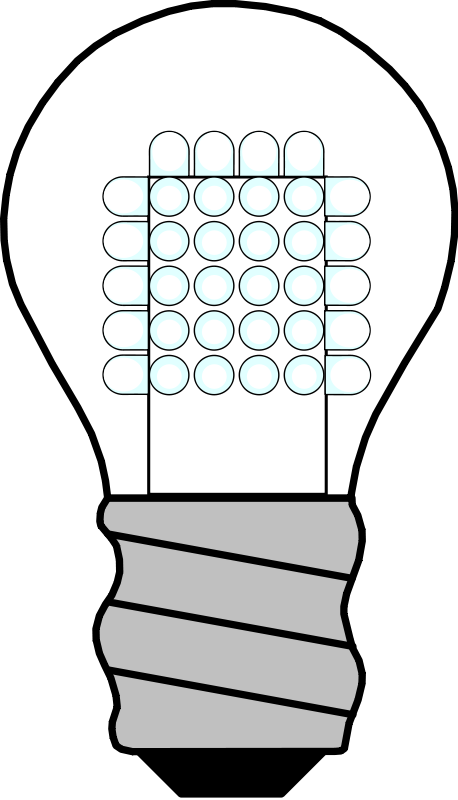
\includegraphics[scale=0.02]{imgs/bulb.png}
 \textbf{Nota} \\
 }%
{\endMakeFramed}

%Work in progress
\newenvironment{workinprogress}{%
  \def\FrameCommand{\colorbox{pink}}%
  \MakeFramed {\FrameRestore}
\lhdbend  \textbf{Work in progress} \\
 }%
{\endMakeFramed}

%Openquestion
\newenvironment{openquestion}{%
  \def\FrameCommand{\colorbox{pink}}%
  \MakeFramed {\FrameRestore}
 \textbf{Domanda aperta} \\
 }%
{\endMakeFramed}

%TODO
\newenvironment{todo}{%
  \def\FrameCommand{\colorbox{pink}}%
  \MakeFramed {\FrameRestore}
 \textbf{TODO} \\
 }%
{\endMakeFramed}

%%%%%%%%%%%%%%%%%%%%%%%%%%%%%%%%
%%%%%%%%%%%% HEADER %%%%%%%%%%%%
%%%%%%%%%%%%%%%%%%%%%%%%%%%%%%%%
\pagestyle{fancy}
% i comandi seguenti impediscono la scrittura in maiuscolo
% dei nomi dei capitoli e dei paragrafi nelle intestazioni
\renewcommand{\chaptermark}[1]{\markboth{#1}{}}
\renewcommand{\sectionmark}[1]{\markright{\thesection\ #1}}
\fancyhf{} % rimuove l'attuale contenuto dell'intestazione
% e del pi\`e di pagina
\fancyhead[LE,RO]{\bfseries\thepage}
\fancyhead[LO]{\bfseries\rightmark}
\fancyhead[RE]{\bfseries\leftmark}
\renewcommand{\headrulewidth}{0.5pt}
\renewcommand{\footrulewidth}{0pt}
\addtolength{\headheight}{0.5pt} % riserva spazio per la linea
\fancypagestyle{plain}{%
\fancyhead{} % ignora, nello stile plain, le intestazioni
\renewcommand{\headrulewidth}{0pt} % e la linea
}


%%%%%%%%%%%%%%%%%%%%%%%%%%%%%%%%
%%%%%%%%%%%% COLORS %%%%%%%%%%%%
%%%%%%%%%%%%%%%%%%%%%%%%%%%%%%%%
\definecolor{code}{gray}{0.3}


%%%%%%%%%%%%%%%%%%%%%%%%%%%%%%%%
%%%%%%%%%%%% NUMBERS %%%%%%%%%%%
%%%%%%%%%%%%%%%%%%%%%%%%%%%%%%%%
\setcounter{tocdepth}{3}
\setcounter{secnumdepth}{3}


%%%%%%%%%%%%%%%%%%%%%%%%%%%%%%%%
%%%%%%%%%%% DOC DATA %%%%%%%%%%%
%%%%%%%%%%%%%%%%%%%%%%%%%%%%%%%%
\title{Appunti di MNO}
\author{Gruppo Informatici Rampanti}
\date{ott 2010 - mag 2011}

\pdfinfo{%
  /Title    (Appunti di MNO)
  /Author   (Andrea Cimino e Lorenzo Muti)
  /Creator  (Andrea Cimino)
  /Producer (Lorenzo Muti)
  /Subject  (MNO)
  /Keywords (MNO)
}


%%%%%%%%%%%%%%%%%%%%%%%%%%%%%%%%
%%%%%%%%%%%%% UTILS %%%%%%%%%%%%
%%%%%%%%%%%%%%%%%%%%%%%%%%%%%%%%
% binary symbols
\newcommand{\modder}{\vdash _{R}}

% vertical gaps
\newcommand{\askip}{\vspace{0.5cm}}
\newcommand{\bskip}{\vspace{1.0cm}}

% various symbols
\newcommand{\qedhere}{\ensuremath{\Box}}
\newcommand{\qed}{\hfill \ensuremath{\Box}}

% substitution
\newcommand{\subst}[2]{^{#1} / _{#2}}

% denotational semantics function names
\newcommand{\bbracket}[1]{\left\llbracket #1 \right\rrbracket}

\newcommand{\aexpr}{\mathcal{A}}
\newcommand{\bexpr}{\mathcal{B}}
\newcommand{\cexpr}{\mathcal{C}}
\newcommand{\Aexpr}[1]{\mathcal{A} \bbracket{#1}}
\newcommand{\Bexpr}[1]{\mathcal{B} \bbracket{#1}}
\newcommand{\Cexpr}[1]{\mathcal{C} \bbracket{#1}}

\newcommand{\semdomset}[1]{(V_{#1})_{\bot}}

% semantic evaluations
\newcommand{\opereval}[3]{\left\langle #1, #2 \right\rangle \rightarrow #3}
\newcommand{\denaeval}[3]{\Aexpr{#1} #2 = #3}
\newcommand{\denbeval}[3]{\Bexpr{#1} #2 = #3}
\newcommand{\denceval}[3]{\Cexpr{#1} #2 = #3}

% rotated sqsubseteqs
\newcommand{\upsqsubseteq}{ $\begin{rotate}{90} $\sqsubseteq$ \end{rotate}$ }
\newcommand{\downsqsubseteq}{ $\begin{rotate}{270} $\sqsubseteq$ \end{rotate}$ }

% Space after paragraph declaration
\makeatletter
\renewcommand\paragraph{\@startsection{paragraph}{4}{\z@}%
  {-3.25ex\@plus -1ex \@minus -.2ex}%
  {1.5ex \@plus .2ex}%
  {\normalfont\normalsize\bfseries}}
\makeatother



% fast theorem and definition
\newcommand{\ftheo}[1]{\colorbox{YellowGreen}{#1}}
\newcommand{\fdefn}[1]{\colorbox{SkyBlue}{#1}}

\theoremstyle{break}
\theoremsymbol{\ensuremath{\clubsuit}}
\theoremseparator{\newline}
\newshadedtheorem{proc}[theo]{Procedura}

% bold math!
\newcommand{\bm}[1]{\mbox{\boldmath{$#1$}}}

\newcommand{\positive}[1]{\textbf{\color{green} +} #1}
\newcommand{\negative}[1]{\textbf{\color{red} -} #1}


\newtheoremlisttype{tab}%
{\begin{tabular*}{\linewidth}{@{}lrl@{\extracolsep{\fill}}r@{}}}%
{##1&##2&##3&##4\\}%
{\end{tabular*}}
%% This is the main doc.
\def \ismaindoc {}

\title{Appunti del corso di \\
\emph{Metodi numerici e ottimizzazione}}
\vfill\vfill

\author{\LaTeX \; Ninjas \\ \\ Andrea Cimino \\
  Marco Cornolti \\
 Emanuel Marzini \\
 Davide Mascitti \\
 Lorenzo Muti\\
 Marco Stronati \\
 \texttt{\{cimino,cornolti,marzini,mascitti,muti,stronati\}@cli.di.unipi.it}
 \thanks{Questo testo \`e sotto \href{http://creativecommons.org/licenses/by-nc-sa/2.5/it/}{Creative Commons Attribution-NonCommercial-ShareAlike License 2.5 Italy} }
}

\date{set 2010-set 2011}




\pdfinfo{%
  /Title    (Appunti del corso di Metodi numerici e ottimizzazione)
  /Author   (Andrea Cimino, Marco Cornolti, Emanuel Marzini, Davide Mascitti, Lorenzo Muti, Marco Stronati)
  /Subject  (Appunti del corso di Metodi numerici e ottimizzazione 2010/2011)
  /Keywords (Pisa Bevilacqua Bigi Metodi Numerici Ottimizzazione)
}

\begin{document}

\maketitle

\tableofcontents

\chapter*{Prologo}
Queste dispense del corso di Metodi Numerici ed Ottimizzazione sono state elaborate durante il corso dell'A.A. 2010/2011, tenuto dal prof. Giancarlo Bigi e dal prof. Roberto Bevilaqua, nel primo anno in cui il corso è stato attivato nel Corso di Laurea Magistrale in Informatica dell'Università di Pisa.

{\em Sono state preparate da alcuni studenti soprattutto per avere una base per studiare il sostanzioso programma,  quindi mancano di organicità e di un linguaggio uniforme. Inoltre nella versione attuale vi sono probabilmente molti errori}. La speranza è che i professori (con l'aiuto degli studenti dei prossimi anni) possano farlo diventare, se non un libro di testo, almeno una dispensa ben fatta.

Il lavoro principale è stato quello di prendere gli appunti delle lezioni in \LaTeX , fatto da Andrea Cimino. Gli appunti sono poi stati sistemati, rielaborati ed integrati da Andrea Cimino, Marco Cornolti, Emmanuel Marzini, Davide Mascitti, Lorenzo Muti, Marco Stronati.

Spesso abbiamo consultato il materiale on--line offerto dai prof. Bevilacqua (parte sui metodi numerici) e Bigi (parte sull'ottimizzazione).

Si ringraziano gli sviluppatori degli strumenti open--source che abbiamo utilizzato per scrivere questa dispensa, in particolare: \LaTeX, Texmaker, Inkscape, Subversion.

Il lavoro -- sia nella versione compilata che nei sorgenti \LaTeX -- è pubblicato sotto licenza Creative Commons Attribuzione--Non commerciale--Condividi allo stesso modo 3.0 Italia (CC BY-NC-SA 3.0).

Chiunque è libero di riprodurre, distribuire, comunicare al pubblico, esporre in pubblico, rappresentare, eseguire e recitare quest'opera.

Chiunque è libero di modificare quest'opera e ridistribuirla, sotto le seguenti condizioni:
\begin{description}
\item[Attribuzione] l'opera derivata deve citare gli autori originali.
\item[Non Commerciale] non si può usare quest'opera né un'opera derivata per fini commerciali.
\item[Condividi allo stesso modo] l'opera derivata deve essere rilasciata sotto una licenza uguale o compatibile con questa.
\end{description}

Maggiori informazioni su \url{http://creativecommons.org/licenses/by-nc-sa/3.0/it/deed.it}

\vspace{1cm}
\begin{flushright}
Pisa, 28 settembre 2011
\end{flushright}

\vfill
\byncsa A. Cimino, M. Cornolti, E. Marzini, D. Mascitti, L. Muti, M. Stronati

\chapter*{Revisione}

Intendo intanto congratularmi con i miei colleghi che hanno dedicato il loro tempo a realizzare questi appunti, cercando di renderli il pi\`u organici e strutturati possibile.

Questi appunti rappresentano un patrimonio per tutti gli studenti che si accingono a sostenere l'esame di Metodi Numerici ed Ottimizzazione e permettono una pi\`u facile comprensione di molti argomenti che possono risultare ostici.

Il mio compito \`e stato quello di revisionare questi appunti al fine di correggere tutti gli errori che ho incontrato durante lo studio, che fossero semplici errori grammaticali o errori all'interno di formule e dimostrazioni.

Purtroppo risulta molto complesso individuare tutti gli errori in una raccolta cos\`i vasta, per cui confido che qualche studente possa avere lo stimolo a continuare il lavoro che ho iniziato.

\`E per questo motivo che ho deciso di raccogliere tutti gli appunti in un repository \texttt{git}: \url{http://github.com/cortinico/mno-notes}
e di renderli disponibili pubblicamente, in modo che chiunque possa utilizzarli e modificarli. Ho incluso nel repository un breve \texttt{README} che descrive le modalit\`a con cui \`e possibile contribuire.

Ringrazio nuovamente i veri autori di quest'opera e, secondo le loro volont\`a, la redistribuisco coperta da licenza Creative Commons Attribuzione--Non commerciale--Condividi allo stesso modo 3.0 Italia (CC BY-NC-SA 3.0).

\vspace{1cm}
\begin{flushright}
Pisa, 20 febbraio 2015
\end{flushright}

\vfill
\byncsa N. Corti


 %% Copyright (C) 2011, Andrea Cimino, All Rights Reserved.
 %% This file is distributed under the terms of the Creative Commons
 %% Licence Non-Commercial Share-Alike license


% \chapter{Capitolo 1:Introduzione}
% %%  22 Ottobre 2010
% \section{Valutazione Riviste}
% Due indici per riviste scientifiche: vogliamo stabilire se esiste una certa correlazione.
% Problema dei minimi quadrati: trovare il valore di $p$ e $q$ tale per cui
% riusciamo a minimizzare la quantità.  (Problema di ottimizzazione non vincolata). 
% $$ \displaystyle \sum_{i=1}^{n}$$
% 
% Abbiamo ricondotto tale problema ad un problema di \emph{minimizzazione}.
% 
% \section{Decadimento esponenziale}
%  $$ y(t) = \theta e^{-\lambda t} $$
% Applicazioni in:
% \begin{itemize}
%  \item fisica
%  \item chimica
%  \item farmacologia
%  \item economia
%  \item informatica (BGP (\emph{border gateway protocol}): routing flapping mapping)
% \end{itemize}
% Nei primi 3 settori non si conoscono tali parametri. Nella fisica però è possibile
% fare delle misurazioni (osservazioni sperimentali).
% Per sapere quali sono i parametri $\lambda$ e $\theta$ procediamo risolvendo il
%  problema dei minimi quadrati.  (Problema di ottimizzazione vincolato). 
% $$ \displaystyle \sum_{i=1}^{n} \left( y_i - \theta e^{-\lambda t_i}\right)^{2} \quad : \quad \theta, \lambda > 0$$
% 
% 
% \section{Compressione delle immagini}
% Immagine rappresentata da una matrice $m \times n$ che contiene $m \cdot n$ valori, i quali codificano
% i livelli di grigio. Costo dell'ingombro: $m \cdot n \cdot \cdot \underbar{c}$. $c$ è il numero di bit
% che codifica il livello di grigio. Abbiamo due scelte per ridurre il costo:
% \begin{itemize}
%  \item Ridurre $m \cdot n$
%  \item Ridurre $c$
% \end{itemize}
% Se la matrice $A$ avesse rango $1$ (le righe o le colonne sono proporzionale fra loro).
% Tali matrici possono essere scritto come un prodotto di vettore riga per il prodotto di un
% vettore colonna. In questo modo passiamo da un costo (per l'occupazione di spazio)
% quadratico ad un costo lineare.
% %%$$A =  \sum_{i=1)^{n} c_i$$ n matrici di rango 1.
% Se invece di avere $n$ riuscissimo ad avere un numero basso di matrici di rango 1,
% ridurremmo il costo a $k(2n)$.
% 
% 
% SVD : Decomposizione a valori singolari
% 
% Una matrice (vedendola quadrata) puoò essere vista nel seguente modo:
% $$ A =  U \Sigma V^{H} $$ 
% dove
% \begin{itemize}
%  \item $U$ è la matrice unitaria
%  \item $\Sigma$ contiene numeri positivi reali che sono i valori singlolari
%  \item $V^{H}$: unitaria.
% \end{itemize}
% Ma
% $$ A =  U \Sigma V^{H}  = \Sigma_{i=1}^{n} \sigma_i \mu_i v_i^{H}$$
% Le Matrici unitarie hanno modulo $\geq 1$.
% Riusciamo a prendere un $k$ abbastanza basso che all'occhio approssima la matrice originaria. \\ \\
% Altri algoritmi (JPEG), agiscono su sottomatrici, localmente. 
% 
% \section{Classificazione supervisionata}
% $\{ x_1, \ldots, x_n \}, \{ y_1, \ldots , y_m\} \subseteq R^n: x_i \text{dati positivi}, x_i \text{ dati negativi}$ \\
% è possibili discriminare i due insiemi? \\ \\
% Classificazione: trovare $f: R^n \rightarrow R $tale che 
% \begin{itemize}
%  \item $f(x_i) > 0 \quad i =1, \ldots, n$
%  \item $f(y_j) < 0 \quad j =1, \ldots, m $
% \end{itemize}
% Spazio di ricerca : $f(x) = a^{T}x -b \quad a \in R^{n}, b \in R$ \\ \\
% Classificazione lineare: torvare $a \in R^{n}, b \in R$ tali che
% \begin{itemize}
%  \item $a^{t} x_i > 0 \quad i =1, \ldots, n$
%  \item $a^{t} y_j < 0 \quad j =1, \ldots, m$
% \end{itemize}
% In alcuni casi non è possibile separe i quadratini dalle crocette. \\
% Obiettivo: trovare la migliore retta che classifichi i due insiemi (margine più grande). \\ \\
% Vogliamo massimizzare quindi tale margine:
%  \begin{itemize}
%   \item $ a^T x_i \geq b+t \quad i = 1, \ldots, n$ 
%  \item $ a^T y_j \leq b -t \quad j = 1, \ldots, m$
%  \end{itemize}
% Il Problema correspondente di programmazione (non lineare) è:
%  \begin{itemize}
%  \item max t
%   \item $ a^T x_i - b \geq t \quad i = 1, \ldots, n$ 
%  \item $ a^T y_j  -b \leq -t \quad j = 1, \ldots, m$
%  \item $$ || a ||_{2} \leq 1 $$ (norma)
%  \end{itemize}
% Se il valore ottimo è positivo, ovvero i due insieme possono essere
% discriminati, il problema è equivalente (con $a' = a/t$ e $b' = b/t$) a:
%  \begin{itemize}
%  \item $min ||a'||_{2}$
%   \item $ a^T x_i -b' \geq 1 \quad i = 1, \ldots, n$ 
%  \item $ a^T y_j -b'\leq 1 \quad j = 1, \ldots, m$
%  \end{itemize}
% Lo norma non è lineare.
% 
% \section{La matrice di Google (PageRank)}
% Si devono ordinare tutte le pagine del web in base alla loro importanza.
% Come definire l'importanza di una pagina?
% Possibile scelta per un modello: \emph{l'importanza di una pagina 
% dipende dall'importanza delle pagine che puntano alla pagina stessa}. \\ \\
% Si numerano le pagine del web da $1$ a $n$.
% Si definisce la matrice di connettivita H:
% H = [h11......h_1n
% 
% 
%     h_n1..     h_nn]
% Ad esempio, per $n= 4$, si consideri il web descritto dal grafo e dalla matrice
% di connettività seguenti
% 
%  0 1 1 1
%  1 0 0 1
%  0 0 0 1
%  0 1 1 0
% 
% La pagina $i$ trasmette la sua importanza alle pagine da essa puntate
% corrispondenti agli elementi non nulli della riga $i$-esima di $H$. \\
% Per Ripartire tale importanza uniformemente tra le pagine
% puntate: al generico link $ i \rightarrow j$ si associa il peso $1/r_i$.
% \\
% Nell'esempio si ottene dalla matrice H la matrice scalata er le righe:
% 
% diag (r_1 r_2 r_3 r_4) =
%   [ 0    1/3  1/3 1/3
%    1/2   0     0   1/2
%    0     0     0     1
%    0     1/2   1/2   0 ]
% 
% In generale, la matrice diag(r_1 \ldots r_n)H ha la proprietà di avere
% le righe con somma 1 e si dice \emph{stocastica per righe}
% 
% Proprieta: una matrice stocastica (per righe o per colonne) ammette autovalore 1.
% 
% 
% Se si indica con $x_j$ l'importanza della pagina $j$ deve essere
%  $$ x_j = \frac{h_1j}{r_1}x_1 + \ldots +  \frac{h_nj}{r_n}x_n  \quad \text{per } j = 1,2, \ldots, n$$
% ovvero 
% $$ x^{T} = x^{T} DH $$
% dove $D = diag(r1 \ldots r_n) $
% Il sistema pu`\o essere riscritto nelle forme seguenti:
% 
%  $$ x = H^{t}Dx $$
% $$ (H^{t}D = I) x = 0$$
% La matrice $H^{T} D =I $ è singolare perchè $H^{T}D$ è stocastica per
% colonne e quindi ammette autovalore 1. Si dimostra che: \\
%  un autovalore di modulo massimo, cioè
% 
% 
% per l'autovalore 1 esistono autovettori non negativi.
% 
% 
% Tra le initie soluzioni del sistema $(H^{T}D -I) x = 0$ si 
% considerino quelle non negative, 
% 
% 
% 
% 
% Il modello matematico può essere migliorato. \\
% Gli elementi di $DH$ posso essere visti come probabilità.
% 
% Si vuole permettere che, con un valore di probabilità piccolo\\
% prestabilito, il navigatore salti dalla pagina dove si trova a una
% qualunque altra. Nel modello:
% Ciò significa sostituire tutti gli zeri.
% 
% La matrice G:
% \begin{itemize}
%  \item è stocastica per righe;
%  \item è irriducibile;
%  \item bla;
% \end{itemize}
% Per risolvere tala problema si può utiizzare col metodo delle potenze
% applicato a $G^T$.
% 
% \section{Configurazione di molecole}
% Potenziale di Lennard-Jones:
%   $$ V(r) = 4 \varepsilon [ (\sigma/r)^{12} - (\sigma/r)^{6} ] $$
% Molecola di $n$ atomi : $x_i \in R^3$ posizione nello spazio dell'atomo $i$
%  $$ E[x_1, \ldots, x_n] = \sum_{i<j} 4 \varepsilon   [ (\sigma/r)^{12} - (\sigma/r)^{6} ] $$
% dove $r_{ij} = || x_i - x_j ||_{2} $ la distanza tra gli atomi $i$ e $j$ \\
% Configurazione di molecole ad energia potenziale minima:
% $$  $$

%%% Local Variables: 
%%% mode: latex
%%% TeX-master: t
%%% End: 
 %% Introduzione corso
 %% Copyright (C) 2011, Andrea Cimino, All Rights Reserved.
 %% This file is distributed under the terms of the Creative Commons
 %% Licence Non-Commercial Share-Alike license

%%26 Ottobre
%% Useful stuff for separate compilation.
\ifx\ismaindoc\undefined
\providecommand{\inbpdocument}{
 \documentclass[11pt,a4paper,twoside,titlepage]{scrbook}
%%%%%%%%%%%%%%%%%%%%%%%%%%%%%%%%
%%%%%%%%%%% PACKAGES %%%%%%%%%%%
%%%%%%%%%%%%%%%%%%%%%%%%%%%%%%%%
% encoding
\usepackage[utf8x]{inputenc}
\usepackage[italian]{babel} % babel (suddivisione parole in sillabe)

\usepackage{amsfonts} % matematica
\usepackage{amsmath} % matematica
\usepackage{amssymb} % simboli vari
\usepackage{calrsfs}
\usepackage{caption}
\usepackage{enumerate}
\usepackage{extarrows} % matematica
\usepackage{keyval}
\usepackage{manfnt} % Simboli curva
\usepackage{mathtools} % matematica
\usepackage{multirow} 
\usepackage[usenames, dvipsnames]{color} % colori con nome
\usepackage[pdftex]{graphicx}
\usepackage{epstopdf} % gestione file EPS
\usepackage{wrapfig} % per figure circondate da testo
\usepackage{framed}	% teoremi framed
\usepackage{fancyhdr} % header buffi
\usepackage[T1]{fontenc} % gestione hbox e vbox
\usepackage[a4paper]{geometry}
\usepackage{microtype} % gestione hbox e vbox
\usepackage[thref, amsthm, amsmath, framed, hyperref]{ntheorem} % teoremi (avanzata)
%% \usepackage{prooftree} % gestione prof-tree
\usepackage{rotating}
\usepackage{stmaryrd}
\usepackage{subfig}
\usepackage{syntax} % syntattic stuff
\usepackage{txfonts}
\usepackage{verbatim} % migliorie al verbatim
%\usepackage{hyperref}
%% \usepackage{qtree}
\usepackage{fancyvrb}
\usepackage{listings}
\usepackage{cancel}
\usepackage{tikz}

\usepackage{bbding} %% Icons

%%%%%%%%%%%%%%%%%%%%%%%%%%%%%%%%
%%%%%%%%%%% GEOMETRY %%%%%%%%%%%
%%%%%%%%%%%%%%%%%%%%%%%%%%%%%%%%
\geometry{verbose,tmargin=2cm,bmargin=2.5cm,lmargin=2.5cm,rmargin=2cm}
\parindent0ex %% Remove paragraph indenting

%%%%%%%%%%%%%%%%%%%%%%%%%%%%%%%%
%%%%%%%%%%% CODE ENV %%%%%%%%%%%
%%%%%%%%%%%%%%%%%%%%%%%%%%%%%%%%
% codice
\newcounter{count}
\setcounter{count}{0}
\newenvironment{code}[1]
{
\color{lightgray}\hrulefill\color{code}
\stepcounter{count} {\bf\small Listato di codice \arabic{count}: {#1} }
\verbatim
}
{
\endverbatim
\color{lightgray}\hrulefill
\color{black}
\\
}

% codice semplice
\newenvironment{simplecode}
{
\color{code} \tt
}
{
\rm
}

 % Notation issues
\input{macros}

\makeatletter
\g@addto@macro\@verbatim\footnotesize
\makeatother



%%%%%%%%%%%%%%%%%%%%%%%%%%%%%%%%
%%%%%%%% THEOREMS FORMAT %%%%%%%
%%%%%%%%%%%%%%%%%%%%%%%%%%%%%%%%
% shaded theorems and proofs command
\definecolor{lightgray}{RGB}{230,230,230}
\def\theoremframecommand{\colorbox{lightgray}}

%%% theorems
\theoremstyle{break}
\theoremheaderfont{\normalfont\bfseries}
\theorembodyfont{\itshape}
\theoremsymbol{\ensuremath{\diamondsuit}}
\theoremseparator{\newline}
\newtheorem{theo}{
\includegraphics[scale=0.11]{imgs/book.png}Teorema}[chapter]

%%% propositions
\theoremstyle{break}
\theoremheaderfont{\normalfont\bfseries}
\theorembodyfont{\itshape}
\theoremsymbol{\ensuremath{\diamondsuit}}
\theoremseparator{\newline}
\newshadedtheorem{proposition}{Proposizione}[chapter]

%%% exercises
\theoremstyle{break}
\theoremheaderfont{\normalfont\bfseries}
\theorembodyfont{\itshape}
\theoremsymbol{\ensuremath{\diamondsuit}}
\theoremseparator{\newline}
\newshadedtheorem{exercise}{Esercizio}[chapter]

%%% propositions
\theoremstyle{break}
\theoremheaderfont{\normalfont\bfseries}
\theorembodyfont{\itshape}
\theoremsymbol{\ensuremath{\diamondsuit}}
\theoremseparator{\newline}
\newshadedtheorem{property}{\PencilRightDown $\; $ Propriet\`a}[chapter]

%%% lemmas
\theoremstyle{break}
\theoremheaderfont{\normalfont\bfseries}
\theorembodyfont{\itshape}
\theoremsymbol{\ensuremath{\diamondsuit}}
\theoremseparator{\newline}
\newshadedtheorem{lemma}[theo]{Lemma}

%%% definitions
\theoremstyle{break}
\theoremsymbol{\ensuremath{\clubsuit}}
\theoremseparator{\newline}
\newshadedtheorem{defn}[theo]{Definizione}

%%% examples
\theoremstyle{break}
\theorembodyfont{\itshape}
\theoremsymbol{\ensuremath{\ast}}
\theoremseparator{\newline}
\newshadedtheorem{example}[theo]{Esempio}

%%% observations
\theoremstyle{break}
\theorembodyfont{\itshape}
\theoremsymbol{\ensuremath{\ast}}
\theoremseparator{\newline}
\newshadedtheorem{observation}[theo]{

\includegraphics[scale=0.06]{imgs/lens.png}
Osservazione
}

%%% notations
\newtheorem*{notaz}{Notazione}

%%% proofs
\newenvironment{thproof}
{
\vskip 0.03cm
\begin{small}
\textit{Dimostrazione. }
\color{code}
}
{
\color{black}
\end{small}
$ \square $
\vskip 0.2cm
}

%Notes
\newenvironment{notes}{%
  \def\FrameCommand{\colorbox{yellow}}%
  \MakeFramed {\FrameRestore}
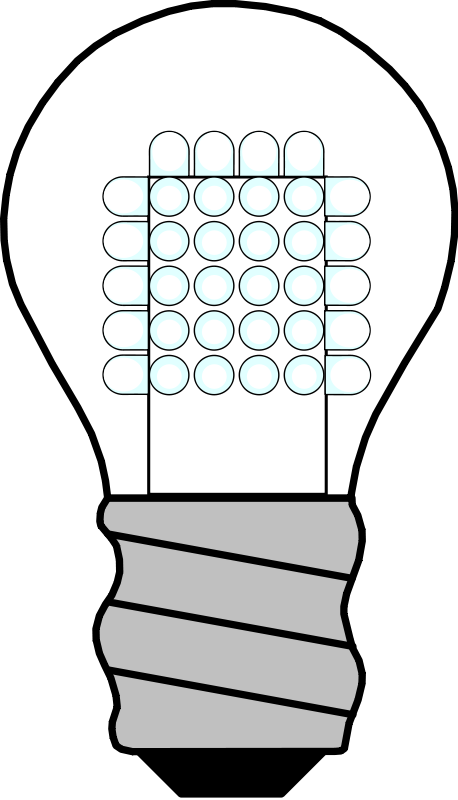
\includegraphics[scale=0.02]{imgs/bulb.png}
 \textbf{Nota} \\
 }%
{\endMakeFramed}

%Work in progress
\newenvironment{workinprogress}{%
  \def\FrameCommand{\colorbox{pink}}%
  \MakeFramed {\FrameRestore}
\lhdbend  \textbf{Work in progress} \\
 }%
{\endMakeFramed}

%Openquestion
\newenvironment{openquestion}{%
  \def\FrameCommand{\colorbox{pink}}%
  \MakeFramed {\FrameRestore}
 \textbf{Domanda aperta} \\
 }%
{\endMakeFramed}

%TODO
\newenvironment{todo}{%
  \def\FrameCommand{\colorbox{pink}}%
  \MakeFramed {\FrameRestore}
 \textbf{TODO} \\
 }%
{\endMakeFramed}

%%%%%%%%%%%%%%%%%%%%%%%%%%%%%%%%
%%%%%%%%%%%% HEADER %%%%%%%%%%%%
%%%%%%%%%%%%%%%%%%%%%%%%%%%%%%%%
\pagestyle{fancy}
% i comandi seguenti impediscono la scrittura in maiuscolo
% dei nomi dei capitoli e dei paragrafi nelle intestazioni
\renewcommand{\chaptermark}[1]{\markboth{#1}{}}
\renewcommand{\sectionmark}[1]{\markright{\thesection\ #1}}
\fancyhf{} % rimuove l'attuale contenuto dell'intestazione
% e del pi\`e di pagina
\fancyhead[LE,RO]{\bfseries\thepage}
\fancyhead[LO]{\bfseries\rightmark}
\fancyhead[RE]{\bfseries\leftmark}
\renewcommand{\headrulewidth}{0.5pt}
\renewcommand{\footrulewidth}{0pt}
\addtolength{\headheight}{0.5pt} % riserva spazio per la linea
\fancypagestyle{plain}{%
\fancyhead{} % ignora, nello stile plain, le intestazioni
\renewcommand{\headrulewidth}{0pt} % e la linea
}


%%%%%%%%%%%%%%%%%%%%%%%%%%%%%%%%
%%%%%%%%%%%% COLORS %%%%%%%%%%%%
%%%%%%%%%%%%%%%%%%%%%%%%%%%%%%%%
\definecolor{code}{gray}{0.3}


%%%%%%%%%%%%%%%%%%%%%%%%%%%%%%%%
%%%%%%%%%%%% NUMBERS %%%%%%%%%%%
%%%%%%%%%%%%%%%%%%%%%%%%%%%%%%%%
\setcounter{tocdepth}{3}
\setcounter{secnumdepth}{3}


%%%%%%%%%%%%%%%%%%%%%%%%%%%%%%%%
%%%%%%%%%%% DOC DATA %%%%%%%%%%%
%%%%%%%%%%%%%%%%%%%%%%%%%%%%%%%%
\title{Appunti di MNO}
\author{Gruppo Informatici Rampanti}
\date{ott 2010 - mag 2011}

\pdfinfo{%
  /Title    (Appunti di MNO)
  /Author   (Andrea Cimino e Lorenzo Muti)
  /Creator  (Andrea Cimino)
  /Producer (Lorenzo Muti)
  /Subject  (MNO)
  /Keywords (MNO)
}


%%%%%%%%%%%%%%%%%%%%%%%%%%%%%%%%
%%%%%%%%%%%%% UTILS %%%%%%%%%%%%
%%%%%%%%%%%%%%%%%%%%%%%%%%%%%%%%
% binary symbols
\newcommand{\modder}{\vdash _{R}}

% vertical gaps
\newcommand{\askip}{\vspace{0.5cm}}
\newcommand{\bskip}{\vspace{1.0cm}}

% various symbols
\newcommand{\qedhere}{\ensuremath{\Box}}
\newcommand{\qed}{\hfill \ensuremath{\Box}}

% substitution
\newcommand{\subst}[2]{^{#1} / _{#2}}

% denotational semantics function names
\newcommand{\bbracket}[1]{\left\llbracket #1 \right\rrbracket}

\newcommand{\aexpr}{\mathcal{A}}
\newcommand{\bexpr}{\mathcal{B}}
\newcommand{\cexpr}{\mathcal{C}}
\newcommand{\Aexpr}[1]{\mathcal{A} \bbracket{#1}}
\newcommand{\Bexpr}[1]{\mathcal{B} \bbracket{#1}}
\newcommand{\Cexpr}[1]{\mathcal{C} \bbracket{#1}}

\newcommand{\semdomset}[1]{(V_{#1})_{\bot}}

% semantic evaluations
\newcommand{\opereval}[3]{\left\langle #1, #2 \right\rangle \rightarrow #3}
\newcommand{\denaeval}[3]{\Aexpr{#1} #2 = #3}
\newcommand{\denbeval}[3]{\Bexpr{#1} #2 = #3}
\newcommand{\denceval}[3]{\Cexpr{#1} #2 = #3}

% rotated sqsubseteqs
\newcommand{\upsqsubseteq}{ $\begin{rotate}{90} $\sqsubseteq$ \end{rotate}$ }
\newcommand{\downsqsubseteq}{ $\begin{rotate}{270} $\sqsubseteq$ \end{rotate}$ }

% Space after paragraph declaration
\makeatletter
\renewcommand\paragraph{\@startsection{paragraph}{4}{\z@}%
  {-3.25ex\@plus -1ex \@minus -.2ex}%
  {1.5ex \@plus .2ex}%
  {\normalfont\normalsize\bfseries}}
\makeatother



% fast theorem and definition
\newcommand{\ftheo}[1]{\colorbox{YellowGreen}{#1}}
\newcommand{\fdefn}[1]{\colorbox{SkyBlue}{#1}}

\theoremstyle{break}
\theoremsymbol{\ensuremath{\clubsuit}}
\theoremseparator{\newline}
\newshadedtheorem{proc}[theo]{Procedura}

% bold math!
\newcommand{\bm}[1]{\mbox{\boldmath{$#1$}}}

\newcommand{\positive}[1]{\textbf{\color{green} +} #1}
\newcommand{\negative}[1]{\textbf{\color{red} -} #1}


\newtheoremlisttype{tab}%
{\begin{tabular*}{\linewidth}{@{}lrl@{\extracolsep{\fill}}r@{}}}%
{##1&##2&##3&##4\\}%
{\end{tabular*}}
\begin{document}
}
\providecommand{\outbpdocument}{\end{document}}
\else
\providecommand{\inbpdocument}{}
\providecommand{\outbpdocument}{}
\fi



\inbpdocument 

\chapter{Richiami di Algebra Lineare}

\section{Richiami su matrici}
Le matrici alle quali ci riferiremo saranno definite su campo dei complessi
 $\mathbb{C}$.\\
Lavoreremo quindi con dei vettori su
$\mathbb{C}$ : $v \in \mathbb{C}^h$, $A \in \mathbb{C}^{m \times n}$.

\subsection{Proprietà importanti sulle matrici}
\begin{defn}[Sottoinsieme chiuso rispetto alla moltiplicazione]
Un sottoinsieme di $C^{n\times n}$ si dice chiuso rispetto
all'operazione di moltiplicazione, se date due matrici $A$ e $B$ 
appartenenti al sottoinsieme, anche il
prodotto $AB$ appartiene al sottoinsieme. 
\end{defn}
I seguenti sottoinsiemi di
 $C^{n\times n}$ sono chiusi rispetto all'operazione di moltiplicazione:
\begin{itemize}
 \item matrici triangolari superiori (inferiori),
 \item matrici triangolari superiori (inferiori) in senso stretto
 \item matrici unitarie
\end{itemize} 
La moltiplicazione fra matrici gode della proprietà associativa, di quella
distributiva rispetto all’addizione, ma non di quella commutativa.

\begin{property}[Propriet\`a sul prodotto di matrici]
  \begin{itemize}
  \item  $A+ 0 = 0 + A = A$  (la matrice nulla \`e l'elemento neutro 
     della somma)
\item $ A+(-A) = 0$ (esistenza di un elemento opposto per la somma)
\item$ (A+ B) + C = A + (B+C)$ (propriet\`a associativa della somma)
\item $  A + B = B + A$   (propriet\`a commutativa della somma)
\item  $(AB)C = A(BC)$   (propriet\`a associativa del prodotto)
\item $ (A+B)C = AC + BC $ (propriet\`a distributiva)
\item $C(A+B) = CA + CB $  (propriet\`a distributiva)
 \end{itemize}
\end{property}

\begin{property}[Sull'inversione di matrici]
Vale la seguente propriet\`a:
$$ (AB)^{-1} = B^{-1} A^{-1}$$
\end{property}

Vale inoltre la seguente propriet\`a
\begin{property}[Reverse order law]
\begin{equation}\label{eq:eq001}  (AB)^{H} =  B^{H} A^{H}\end{equation}
dove $H$ \`e l'operatore di trasposizione coniugata.
\end{property}

\begin{openquestion}
Quali condizioni sono necessarie affinch\'e valga la reverse order law?
Una dimostrazione di tale proprietà: \\
si ponga 
$$ M = AB$$
Allora valgono le seguenti implicazioni
$$ A^{-1}M = A^{-1}AB \quad \Rightarrow \quad
 B^{-1}A^{-1}M = B^{-1}B  \quad
 \Rightarrow \quad
 B^{-1}A^{-1}M = I \quad 
$$
Ma allora $M$ deve essere l'inversa di $B^{-1}A^{-1}$, ma $M=AB$. \\
Il punto di questa dimostrazione che non mi \`e chiaro \`e:
quali condizione (ad esempio  sull'invertibilità di $A$ e $B$)
sono necessarie?

Ciuffo: Semplicemente che A e B siano invertibili, altrimenti 
l'operatore di inversa non dà risultati.
\end{openquestion}

\subsection{Alcune classi importanti di matrici}
\subsubsection{Matrici triangolari}
\begin{defn}[Matrice triangolare]
Le matrici triangolari inferiori (superiori) sono matrici quadrate che
hanno tutti gli elementi al di sopra (sotto) della diagonale
principale nulli.
\end{defn}

Il determinante di una matrice triangolare A può essere calcolato come il
prodotto dei sui elementi pricipali.
$$ \det(A) = \Pi_{i=1}^{n} a_{ii} $$ \label{triangolari}

\begin{defn}[Matrice Hessemberg]
\label{def:hessemberg}
Una matrice di Hessenberg \`e una matrice ``quasi'' triangolare. In
particolare \`e detta \emph{superiore} se ha valori pari a zero sotto la prima
sottodiagonale, viceversa nel caso \emph{inferiore}.
\end{defn}

\begin{example}[Hessemberg superiore e inferiore]
\[\begin{pmatrix}
  1 & 4 & 2 & 3 \\
  3 & 4 & 1 & 7 \\
  0 & 2 & 3 & 4 \\
  0 & 0 & 1 & 3 \\
\end{pmatrix}
\qquad
\begin{pmatrix}
  1 & 2 & 0 & 0 \\
  5 & 2 & 3 & 0 \\
  3 & 4 & 3 & 7 \\
  5 & 6 & 1 & 1 \\
\end{pmatrix}\]
\end{example}

\subsubsection{Matrici simmetriche}

\begin{defn}[Matrice simmetrica]
Una matrice simmetrica \`e una matrice quadrata che ha la proprietà di
essere uguale alla sua trasposta. Quindi A \`e simmetrica sse:
$$ A=A^T \qquad \text{cio\`e} \quad a_{ij} = a_{ji}, \; \forall i \forall j. \; a_{ij} \in A$$
\end{defn}

La classe delle matrici simmetriche \`e un sottoinsieme delle
 matrici Hermitiane.\\

\begin{defn}[Matrice trasposta coniugata]
Data una matrice $A \in C^{m \times n}$, si definisce matrice
trasposta coniugata di $A$ la matrice $B \in C^{n \times m}$ tale che
$$b_{ij} = \overline{a_{ji}}$$ 
dove $\overline{a_{ji}}$ \`e il coniugato del numero complesso $a_{ji}$,
e si indica
$$B = A^{H}$$
\end{defn}

\begin{defn}[Matrice Hermitiana]
Una matrice Hermitiana \`e una matrice a valori complessi che coincide
con la propria trasposta coniugata (o matrice aggiunta).
  $$ A = A^{H} $$
\end{defn}

Proprietà importanti di tali matrici:
\begin{itemize}
\item sulla diagonale principale \emph{devono} essere presenti solamente
  numeri reali. 
\item gli autovalori sono reali.
\item se $A$ \`e \emph{reale} hermitiana, allora risulta $A^{T} = A$ ed
\`e detta \emph{simmetrica}.
\end{itemize}

\begin{property}

Se $A \in  C_{n \times n}$ \`e una matrice hermitiana,
 cio\`e $A = A^{H}$, e $\mathbf{x} \in C_n$ , il  numero 
$$ \alpha =  \mathbf{x}^{H} A \mathbf{x}$$
\`e reale. Infatti, poich\'e  $A$ \`e hermitiana, si ha:
$$\overline{\alpha}  = \overline{\mathbf{x}^{H} A\mathbf{x}} =
 (\mathbf{x}^H A\mathbf{x})^H = 
 ((\mathbf{x}^H A)\mathbf{x})^H \underbracket{=}_{\ref{eq:eq001})} 
 \mathbf{x}^{H}(\mathbf{x}^{H}A)^{H} = 
\mathbf{x}^{H}(A^{H}\mathbf{x})=
 \mathbf{x}^H A^{H} \mathbf{x} = \mathbf{x}^H A\mathbf{x}  = \alpha.$$
\end{property}

\begin{example}[Matrice Hermitiana]
$$\begin{pmatrix}
  2   & 3+i \\
  3-i & 4
\end{pmatrix}$$
\end{example}

\subsubsection{Matrici unitarie}
\begin{defn}[Matrice unitaria]
  Una matrice $U$ \`e detta unitaria se soddisfa la condizione:
  $$U^H U = U U^H = I$$
  dove $I$ \`e la matrice identità.
\end{defn}

\paragraph{Proprietà}
\label{prop:unitarie}
\begin{itemize}
\item Dal punto di vista della complessità ottenere l'inversa
  di una matrice, che in generale ha costo cubico in n, per le
  unitarie \`e immediato, dato che $ U^{-1} = U^{H} $.
\item Le matrici unitarie hanno autovalori di modulo 1.
\item $U^{-1}$ \`e ancora una matrice unitaria.
\item Le matrici unitarie sono delle isometrie, o rispettano la norma
  2, ossia
  $$||Ux||_{2} = ||x||_{2}$$ 
  Infatti $|| Ux ||_{2} = \sqrt{x^{h}\underbracket{U^{H}U}_{I}x} = ||x||_{2}$
\item Le matrici unitarie danno garanzia di stabilità in tutti i
  calcoli in cui intervengono.
\item Se $A$ \`e \emph{reale} unitaria, allora $A^{T}A = AA^{T} = I$ ed
  \`e detta \emph{ortogonale}.
\end{itemize}

Inoltre le matrici unitarie su $\mathbb{R}^n$ sono tali che le loro colonne
formano una base ortonormale di $\mathbb{R}^n$, cio\`e per ogni coppia
di vettori della base il loro prodotto scalare \`e zero.\\
\begin{example}
  Ad esempio:
$$
\begin{bmatrix} 
  \cos \alpha & -\sin \alpha \\
  \sin \alpha & \cos \alpha
\end{bmatrix}
$$
\`e una base ortonormale di $\mathbb{R}^{2}$.
\end{example}

\begin{openquestion}
Queste considerazioni valgono anche per $\mathbb{R}$?

Ciuffo: certo che valgono anche per  $\mathbb{R}$: l'unica matrice
 unitaria per $\mathbb{R}$ \`e [1], quindi la proprietà
\`e banalmente dimostrata dato che non ci sono le coppie di colonne 
diverse della matrice per cui dovrebbe valere la proprietà.
\end{openquestion}

\paragraph{Matrici  unitarie importanti}
\subparagraph{Matrici di rotazione piana (2x2)}
Ruota un vettore di un angolo $\theta$
$$
G = 
\begin{bmatrix} 
\cos \theta & -\sin \theta \\
\sin \theta &  \cos \theta 
\end{bmatrix} 
$$

\subparagraph{Matrice di rotazione piana (n x n)}
$$ G =
\begin{bmatrix}
1 & 0 & 0 &...& ... &... & 0 & 0 & 0 \\
0 & 1 & 0 &... & ... &... & 0 & 0 & 0 \\
0 & 0 & ... & ... & ... &... & ...&0 & 0 \\
0 & 0 & ...  & cos(\theta ) &  ... & -sen(\theta ) & ... & 0&0 \\
0 & 0 & ... &  ... & 0 &... & ...& 0& 0 \\
0 & 0 & ... & 0 & 1 & 0 &...&0 &0\\
0 & 0 & ... & ... & 0 &... & ...& 0 & 0 \\
0 & 0 & ...  & sen(\theta ) &  ... & -cos(\theta ) & ...&0 &0 \\
0 & 0 & ... & ... & ... & ... & ...&0 & 0 \\
0 & 0 & 0 &... & ... & ... & 0 & 1 & 0 \\
0 & 0 & 0 &... & ... &... & 0 & 0 & 1 \\
\end{bmatrix}
$$

\subparagraph{Matrice di permutazione}
Una matrice di permutazione $P_{\pi}$, per la permutazione $\pi$ 
si ottiene da $I$ permutandone le righe.
\begin{example}[Matrice di permutazione]
  $$P_{\pi} =
  \begin{bmatrix}
    0 & 0 & 0 & 1  \\
    1 & 0 & 0 & 0  \\
    0 & 1 & 0 & 0  \\
    0 & 0 & 1 & 0  \\
  \end{bmatrix}
  $$
\end{example}

Dato che le matrici di permutazione sono matrici ortogonali, cio\`e
$P_{\pi}P_{\pi}^{T} = I$:

\begin{itemize}
\item sono matrici unitarie
\item l'inversa esiste e si scrive $P_{\pi}^{-1} = P_{\pi^{-1}} = P_{\pi}^{T}$
\end{itemize}

Nel caso di un vettore colonna $x$, $P_{\pi} x$ ne permuta le righe.

\subsection{Prodotto scalare}
\paragraph{su $\mathbb{R}^{n}$}
$$\langle u, v \rangle = \sum_{i=1}^{n} u_{i} v_{i} = u^{T}v$$

Si può inoltre definire la norma euclidea di un vettore tramite il
prodotto scalare in $\mathbb{R}^n$:
$$ || u || = \sqrt{\langle u,u \rangle} = \sqrt{\sum_{i=1}^{n} u_{i}^2} $$

\paragraph{su $\mathbb{C}^{n}$}
$$\langle u, v \rangle = \sum_{i=1}^{n} \overline{u_{i}} v_{i} = u^{H}v$$

Inoltre $u^{H} u = \sum_{i=1}^{n} \bar{u_i}u_i = \sum_{i=1}^{n} |
u_i|^{2}$ e quindi anche in questo caso basta fare la radice quadrata
per ottenere la norma euclidea.
\begin{property}\label{eigenvalues:ei001}
Il prodotto scalare $f(u,v)=\langle u,v \rangle$ su $\mathbb{C}^{n}$ gode
 delle seguenti proprietà:
\begin{itemize}
\item $f(au + bv, w) = af(u,w) + bf(v,w)$
\item $f(u,av + bw) = af(u,w)$
\item $f(u,v) = \overline{f(v,u)}$
\item $f(u,u) \geq 0$ \quad e 
       \quad  $f(u,u) = 0 \; \Longleftrightarrow \; u = 0$
\end{itemize}
\end{property}

Nota: il prodotto di un complesso per il suo coniugato ne dà il modulo
 al quadrato:
$$ (Re(\lambda) + i \; Im(\lambda)) \; (Re(\lambda) - i \; Im(\lambda)) = 
   Re^2(\lambda) + Im^2(\lambda)$$


\subsubsection{Matrici normali}
\begin{defn}[Matrice normale]
Una matrice quadrata $A$ \`e \emph{normale} se
$$ A^H A = A A^H $$
\end{defn}

Questa classe contiene anche le hermitiane e le unitarie, infatti:
\begin{itemize}
\item se una matrice \`e hermitiana allora \`e normale
\item se una matrice \`e unitaria allora \`e normale
\end{itemize}
\begin{property}
Una matrice normale pu\`o essere diagonalizzata per mezzo
di matrici unitarie.
\end{property}


\subsubsection{Matrici definite positive}
\begin{defn}[Matrice definita positiva]
Sia $A \in \mathbb{C}_{n\times n}$ una matrice hermitiana e 
sia $x \in \mathbb{C}_n , x \neq 0$.
Allora se il numero reale $x^{H} Ax > 0$ si dice che la matrice $A$ \`e
definita positiva.
Analogamente:
\begin{itemize}
\item se $x^{H} Ax \geq 0$, \quad A \`e semidefinita positiva
\item se $x^{H} Ax \leq 0$, \quad A \`e semidefinita negativa
\item se $x^{H} Ax < 0$, \quad A \`e definita negativa
\end{itemize}
\end{defn}

Sono una sottoclasse delle hermitiane.

\begin{property}
\label{prop:def-pos}
Una matrice $A^{H}A$ \`e semi-definita positiva.\\
Infatti $x^{H}A^{H} Ax =(Ax)^{H} Ax = || Ax|| \geq 0$
Se $A$ rango massimo allora $A^{H}A$ è definita positiva.
\end{property}


\subsubsection{Matrice partizionata a blocchi}
A volte \`e possibile dividere una matrice in sottomatrici o
\emph{blocchi}, e questo può agevolare delle operazioni come il
prodotto, che può essere ridefinito in termini del prodotto dei
blocchi.

\begin{example}[4 blocchi]
$$
\begin{array}{ll}
A = \left[
  \begin{array}{ccccc}
    & A_{11} & \vline & A_{12} \\
    \hline 
    & A_{21} & \vline & A_{22} \\
  \end{array}
\right]
&
B = \left[
  \begin{array}{ccccc}
    &  B_{11}& \vline & B_{12} \\
    \hline 
    & B_{21} & \vline & B_{22} \\
  \end{array}
\right]
\end{array}
$$

Prodotto:
$$
AB = \left[
  \begin{array}{ccccc}
    & A_{11}B_{11} + A_{12}B_{21} & \vline & A_{11}B_{12} + A_{12}B_{22} & \\
    \hline 
    & A_{21}B_{11} + A_{22}B_{21} & \vline & A_{21}B_{12} + A_{22}B_{22} &
  \end{array}
\right]
$$
\end{example}

Attenzione! I blocchi non sono commutativi! 


\subsubsection{Matrici riducibili}
\begin{defn}[Matrice riducibile]
Una matrice $A$ si dice riducibile se esiste una matrice di
permutazione $\Pi$ tale che
$$
B = \Pi \cdot A \cdot \Pi^{T} =
\left[ 
  \begin{array}{ccc}
    B_{11} & \vline & B_{12} \\ 
    \hline 
    O      & \vline & B_{22}
  \end{array}
\right]
$$
cio\`e con i blocchi diagonali $B_{11}$ e $B_{22}$ quadrati e $B_{21} = 0$.
\end{defn}

Questa proprieta \`e legata alla presenza di elementi nulli nella matrice di
 partenza $A$.\\
Prentendere che gli zeri siano sotto o sopra \`e arbitrario.\\

\paragraph{Matrici riducibili nella risoluzione di sistemi lineari}
Supponiamo $A$ riducibile: vogliamo risolvere il sistema di equazioni
$$Ax = b$$
Allora  
$$
\begin{array}{ll}
\Pi A x = \Pi b & \text{applichiamo permutazione} \\
\underbrace{\Pi A \Pi^{T}}_{B} \Pi x = \Pi b & 
\Pi \quad \text{\`e ortogonale, cio\`e} \quad \Pi \Pi ^{T} = I \\
B \Pi x = \Pi b & \text{ponendo} \quad \Pi x = y \quad \Pi b = c \\
B y = c
\end{array}
$$
Riscrivendo in forma matriciale, enfatizzando il fatto che si lavori
con matrici a blocchi:
$$
\left[
  \begin{array}{ccc}
    B_{11} & \vline & B_{12} \\
    \hline                    
    0      & \vline & B_{22}   
  \end{array}
\right]
\left[
  \begin{array}{c}
    y_1  \\
    \hline
    y_2 
  \end{array}
\right]
=
\left[
  \begin{array}{c}
    c_1  \\
    \hline
    c_2 
  \end{array}
\right]
$$
abbiamo triangolarizzato a blocchi la matrice senza fare calcoli.\\
Ora possiamo risolvere il seguente sistema lineare:
$$
\left\{
  \begin{array}{ll}
    B_{11}y_1 + B_{12}y_2 = c_1 \\
    B_{22}y_{2} = c_2           
  \end{array}
\right.
$$
Per riavere la soluzione originale basta riapplicare la permutazione
$x = \Pi^T y$ (costo zero).\\
Il costo totale di risolvere il nuovo sistema \`e $\frac{n^3}{12}$
contro il costo del normale metodo di Gauss $\frac{n^3}{3}$.

\begin{theo}
Una matrice \`e \emph{riducibile} sse il grafo associato non \`e fortemente
 connesso.
\end{theo}
Un grafo \`e fortemente connesso se da ogni nodo \`e possibile arrivare
 ad ogni altro nodo.
 
%% 29 Ottobre 2010
\section{Autovalori ed autovettori}
\begin{defn}[Autovalore/Autovettore]
\label{def:autovalore}
Siano $A \in \mathbb{C}^{n\times n}$, $x \in \mathbb{C}^{n}, x \neq 0$
e $\lambda \in \mathbb{C}$. Se vale 
$$ Ax = \lambda x $$ 
allora $x$ e $\lambda$ sono detti rispettivamente \emph{autovettore} e
\emph{autovalore} di $A$.
\end{defn}

\begin{defn}[Spettro di A]
Lo spettro di una matrice $A$ \`e costituito dall'insieme
degli autovalori di $A$
\end{defn}

\begin{defn}[Raggio spettrale di A]
Siano $\lambda_1, \ldots, \lambda_n \in \mathbb{C}$ gli autovalori di $A$. \\
Il raggio spettrale di $A$, denotato con $\rho(A)$, \`e 
definito come
$$ \rho(A) = \max_{1, \ldots, n} | \lambda_i| $$ 
\end{defn}

\begin{defn}[Traccia di A]
Sia $A \in \mathbb{C}^{n\times n}$.
Si definisce \emph{traccia} di $A$ la quantit\`a
$$ tr(A) = \displaystyle \sum_{i=1}^{n} a_{ii}$$
\end{defn}

Valgono inoltre le seguenti propriet\`a
\begin{property}
$$ \displaystyle trA = \sum_{i=1}^{n} \lambda_i
\qquad
\displaystyle detA = \prod_{i=1}^{n} \lambda_i$$
\end{property}

Gli autovalori sono le soluzioni dell'
equazione caratteristica $p(\lambda) = 0$,
dove 
\begin{equation}
\label{eigenvalues:eq001}  p(\lambda) = det(A - \lambda I) =
 a_0 \lambda^{n} + a_1 \lambda^{n-1} +  \ldots + a_n 
\end{equation}
In particolare  vale la propriet\`a
\begin{property}
$$ a_1 = -(1)^{n-1}trA \qquad a_n= detA$$
\end{property}
Quindi il tutto può essere riscritto come
$$ p(\lambda)  =  (-1)^n\lambda^{n} + (-1)^{n-1}tr(A)^{n-1}+\ldots+det\; A $$
\`e il polinomio caratteristico di grado $n$. \\

Il problema degli autovalori \`e un problema non lineare e il grado del
polinomio cresce col crescere della dimensione della matrice.\\

Enunciamo inoltre un importante teorema, omettendone la dimostrazione.
Ci sar\`a utile in alcune dimostrazioni
\begin{theo}
  \label{eigenvalues:theo004}
  Una matrice $A$ di ordine $n$ \`e diagonalizzabile se e solo
  se ha $n$ autovettori linearmente indipendenti. Inoltre le colonne
  della matrice $S$, per cui $S^{-1}AS$ \`e diagonale, sono gli autovettori
  di $A$
\end{theo}

\begin{defn}[Sviluppo Laplace]
\label{sviluppo-laplace}
Lo sviluppo di Laplace \`e un metodo di calcolo del \emph{determinante}, che
risulta efficiente per matrici non troppo grandi e sparse. Si procede
scegliendo una riga, la $i$-esima, tramite la formula:

$$ \det(A) = \sum_{j=1}^n\ (-1)^{i + j} a_{i,j} \det(A_{ij}) $$

con $A_{ij}$ la matrice ottenura da $A$ eliminando la riga $i$-esima e la colonna
$j$-esima.

Esiste uno sviluppo analogo anche lungo la j-esima colonna.
\end{defn}


\paragraph{Matrici Hermitiane}
\begin{property}
Se $A$ Hermitiana allora gli autovalori sono reali $(\lambda \in \mathbb{R})$. 
\end{property}

\begin{thproof}
Usando la definizione di autovalore 
$$ Ax = \lambda x \quad \text{con} x \neq 0 $$
Calcolo la trasposta coniugata in entrambi i membri 
$$ x^H A^H = x^H \lambda^H= x^H \overline{\lambda} = \overline{\lambda} x^{H} $$
Moltiplico entrambi i membri per $x$ (diverso da 0 per ipotesi)
$$ x^H A^H x = \overline{\lambda}  x^{H} x \qquad (1) $$
Prendo la definizione di autovalore e moltiplico entrambi i membri per $x^{H}$
$$x^{H} A x = x^{H} \lambda x = \lambda x^{H} x \qquad (2)$$
Dato che A \`e hermitiana (1) e (2) sono uguali, da cui
$$ \lambda x^{H} x = \overline{\lambda} x^{H} x$$
Dato che $x^{H} x \neq 0 \; (\sum |x_i|^{2} \neq 0) $ allora posso
 semplificare, ottenendo
$$ \lambda=\overline{\lambda} \; \Rightarrow \; \lambda \in \mathbb{R} $$
\end{thproof}


\paragraph{Matrici Unitarie}
Verifichiamo gli autovalori per le matrici unitarie:
\begin{property}
Sia $U$ unitaria allora i suoi autovalori hanno modulo 1.
 $$| \lambda | = 1 $$
\end{property}

\begin{thproof}
Sia $\lambda$ un autovalore. Poich\'e per le matrici unitarie vale la
propriet\`a
$$ |Ux| = |x|$$
inoltre vale per definizione
$$  U^{H} U = I$$
Moltiplicando ciascun membro di $Ux = \lambda x$ per se stesso trasposto
 coniugato, usando la reverse order law ({\ref{eq:eq001})}, otteniamo
$$ x^{H} \underbracket{U^{H} U}_{I}x = x^{H}x \overline{\lambda} \lambda 
\quad 
\Rightarrow 
 \quad \underbracket{x^{H}x}_{scalare} = |\lambda|^2 \underbracket{x^{H}x}_{\text{scalare}}  
 \quad \Rightarrow \quad  1 = | \lambda|^{2}$$
\end{thproof}


\paragraph{Autovalori per matrici definite positive}
\begin{property}
$A$ è definita positiva se e solo se
i suoi autovalori sono reali positivi.
\end{property}

\begin{thproof}
Al solito prendiamo la definizione di autovalore
$$ Ax = \lambda x$$
Moltiplicando i due membri per $x^{H}$ a sinistra
$$ x^{H}Ax = x^{H} \lambda x$$
che \`e equivalente a
$$ x^{H}Ax =  \lambda x^{H}  x$$
Utilizzando per ipotesi
\begin{itemize}
\item $x^{H}x > 0 $ per una delle (\ref{eigenvalues:ei001})
\item $x^{H}Ax > 0$ essendo $A$ definita positiva
\end{itemize}
possiamo scrivere
$$ \underbracket{x^{H}Ax}_{>0} =  \lambda \underbracket{x^{H}x}_{>0}$$
Ma allora $\lambda$ deve essere necessariamente positivo
\end{thproof}

Quindi definita positiva implica tutti gli autovalori positivi e vale
anche il viceversa anche se dobbiamo dimostrarlo.\\

\begin{theo}
 \ref{richiamibevilacqua:theo01}
 Una matrice hermitiana A \`e definita positiva se e solo se i
determinanti di tutte le sottomatrici principali di testa di A (e quindi anche
il determinante di A) sono positivi.
\end{theo}

\begin{defn}
  Sottomatrici principali sono quelle matrici create scegliendo
  colonne e righe con gli stessi indici.
\end{defn}

\begin{example}
  Prendendo gli indici 1 e 3 da una matrice 4 x 4 otteniamo una
  sottomatrice principale 2x2 con la diagonale sovrapposta a quella
  della matrice di origine.
\end{example}

%%% Warning: Dimostrazione??? 


\begin{theo}[Teorema di Cayley - Hamilton]
\label{eigenvalues:teo01} 
 Sia $p$ il polinomio caratteristico di $A$ allora
 $$ p(A) = 0$$
\end{theo}
\begin{thproof}
 (Rimandiamo la dimostrazione, quando si parler\`a di diagonalizzazione) 
\end{thproof}
Vediamo per $n = 2$ \\
Il polinomio caratteristico \`e dato da
$$ p(\lambda) = (-1)^{2} \lambda^{2} - tr(A)\cdot \lambda + detA $$
Allora il teorema afferma che per ogni matrice $A$ vale
$$p(A) = A^2 - tr(A) \cdot \lambda + det\; A \cdot I \underbracket{ = 0
} $$
Non \`e ovvio che quello sia 0, \`e quindi un teorema importante.
 \\ \\
Vediamo nel caso $A \quad m \times n$
\begin{equation}
\label{eigenvalues:eq002} 0 = a_{0}A^{n} + a_1 A ^{n-1} \ldots a_{n}I  =  p(A)
\end{equation}
Se $A$ \`e invertibile, moltiplicando per $A^{-1}$ otteniamo
$$ 0 = a_0 A^{n-1} + a_1 A^{n-2} \quad \underline{a_n}A^{-1}$$
$a_n \neq 0$ perch\`e sappiamo che \`e il determinante, quindi
$$ A^{-1} = \frac{1}{a_n}\cdot \left( \text{polinomio in A di grado n-1} \right) $$
\begin{openquestion}
Come \`e stata fatta questo accenno alla matrice inversa?
Cosa si voleva fare vedere? Si voleva fare vedere per
caso che $1/a_{n}$ \`e un autovaolre di $A^{-1}$
\end{openquestion}
Non serve considerarare polinomi in una matrice di grado troppo elevato
 (maggiore o uguale a $n$) \\
Sia $S$ un polinomo di grado $m \geq n$ dove $n$ \`e l'ordine della matrice.
Allora 
$$ \underbracket{S(x)}_{m}  = \underbracket{p(x)}_{n}\underbracket{q(x)}_{m-n} + \underbracket{r(x)}_{< n} \quad \text{divisione fra polinomi} $$
$$S(A) = \underbracket{\cancel{p(A) q(A)}}_{=0 \;(\ref{eigenvalues:teo01})} + r(A) = 0$$
Quindi abbiamo un poilinomio di grado $< n$ \\
C'\`e un polinomio (polinomio minimo): \`E possibile che esistano altri
 polinomi $S(\lambda)$
con $S(A) = 0$ e grado minore di $n$
\begin{defn}[Polinomio minimo]
Si definisce polinomio minimo $\psi(\lambda)$ il polinomio monico 
(ossia con primo coefficiente uguale a 1) di grado minimo tale che
 $\psi(A) = 0$ (matrice nulla)
\\ From Wikipedia\\ \\
Data una matrice quadrata $A$ a valori in un certo campo $K$, si considera
l'insieme $$ I = \{p\in K[x]\ |\ p(A) = 0\} $$
di tutti i polinomi che annullano $A$. Questo insieme risulta essere
un ideale nell'anello $K[x]$ di tutti i polinomi con coefficienti in $K$.
\\ \\
L'anello $K[x]$ \`e un anello euclideo: \`e infatti possibile fare una
divisione fra polinomi con resto. Conseguentemente, \`e un anello ad
ideali principali: ogni ideale \`e generato da un unico elemento. 
In particolare, :$I = (m(x))\,\!$ 
\`e generato da un elemento $m(x)$. Tale elemento \`e unico solo a meno 
di moltiplicazione per una costante non nulla: \`e quindi unico se lo si 
suppone ''monico'' (cio\`e con coefficiente 1 nel termine $x^k$ più grande).
Si definisce quindi il '''polinomio minimo''' di $A$ tale polinomio $m(x)$.
\end{defn}
\begin{example}
 $$A = I_{n} $$
 $$ P(\lambda ) = (1-\lambda)^{n} \qquad  det(I - \lambda I) = 
\left[
\begin{array}{cc}
 ( 1 - \lambda  & 0 \\
0   & 1-\lambda)
\end{array}
\right]
 $$
 $$ \psi(\lambda) = -(1 -\lambda) = \lambda -1 $$
$$ \psi(I) = I - I = 0$$           
\end{example}
\begin{example}
 From Wikipedia \\
Consideriamo per esempio la matrice 
$$A = \begin{bmatrix}1&2\\
3&4\end{bmatrix}$$
Il suo polinomio caratteristico \`e dato da

$$p(\lambda)=\det\begin{bmatrix}1-\lambda&2\\
3&4-\lambda\end{bmatrix}=(1-\lambda)(4-\lambda)- 2\cdot 3=\lambda^2-5\lambda-2.$$
Il teorema di Cayley–Hamilton sostiene che:
$$A^2-5A-2I_2=0\,\!$$
il che si può facilmente verificare.
\end{example}

\section{Forme canoniche}
\begin{defn}[Matrici simili]
Due matrici quadrate $A$ e $B$ si dicono simili
se esiste una matrice $M$ invertibile per cui vale
$$ A = M^{-1}BM$$
\end{defn}
\`e facile verificare quindi che la similitudine fra matrici
\`e una relazione di equivalenza nell'insieme delle matrici
$M_{n \times n}$
\begin{property}
Matrici simili godono delle seguenti propriet\`a:
\begin{itemize}
 \item hanno stesso rango;
 \item hanno stessa traccia;
 \item hanno stesso determinante;
 \item hanno stesso polinomio caratteristico: questo implica
       che due matrici simili hanno stessi autovalori.
\end{itemize}
\end{property}

\begin{defn}[Molteplicit\`a algebrica e geometrica]
Sia $\lambda_i$ un autovalore di una matrice $A$.\\
Diremo \emph{molteplicit\`a algebrica} di $\lambda_i$
la sua molteplicit\`a nel poliniomo caratteristico. \\
Diremo inoltre \emph{molteplicit\`a geometrica} di $\lambda_i$
la dimensione del relativo autospazio $V_{\lambda_i}$
\end{defn}
Da ricordarsi che una matrice \`e diagonalizzabile se e solo
se molteplicit\`a algebrica e geometrica coincidono. Se non fosse
così, ricordando che la molteplicit\`a algebrica \`e sempre
maggiore o uguale a quella geometrica, possiamo cercare di ricondurre
una data matrice, ad una matrice che abbia una struttura simile
a quella di una matrice diagonale, ed \`e detta forma canonica
di Jordan. Ogni matrice quadrata \`e riconducibile a forma
di Jordan.

\subsection{Forma canonica di Jordan}
La forma canonica di Jordan di una matrice quadrata $A$ definisce una
matrice triangolare $J$ \emph{simile} ad $A$ che ha una struttura il
più possibile vicina ad una matrice diagonale. La matrice \`e diagonale
se e solo se A \`e diagonalizzabile, altrimenti \`e divisa in blocchi
detti blocchi di Jordan.\\

La forma canonica caratterizza univocamente la classe di similitudine
di una matrice, cio\`e due matrici sono simili se e solo se hanno la
stessa forma di Jordan (a meno di permutazione dei blocchi).\\

\paragraph{Blocco di Jordan}
Un \emph{blocco di Jordan} di ordine $k$ \`e una matrice triangolare
superiore con $k$ righe costituita nel seguente modo:
$$
\begin{pmatrix}
 \lambda & 1      & 0      & \cdots & 0      \\                       
 0       & \ddots & \ddots &        & \vdots \\
 \vdots  & \ddots & \ddots & \ddots & 0      \\
 \vdots  &        & \ddots & \ddots & 1      \\
 0       & \cdots & \cdots & 0      & \lambda    
\end{pmatrix}
$$

in cui ogni elemento della diagonale \`e uguale a $\lambda$ ed in ogni
posizione (''i'', ''i''+1) si trova un 1. Il suo polinomio
caratteristico \`e $ (x-\lambda)^k $, e quindi ha $\lambda$ come unico
autovalore con molteplicit\`a algebrica $k$.      \\
D'altra parte, l'autospazio relativo a $\lambda$ \`e:
$$ \ker(J_k(\lambda) - \lambda I) = \ker\begin{pmatrix}
 0      & 1      & 0      & \cdots & 0          \\                       
 0      & \ddots & \ddots &        & \vdots     \\
 \vdots & \ddots & \ddots & \ddots & 0          \\
 \vdots &        & \ddots & \ddots & 1          \\
 0      & \cdots & \cdots & 0      & 0    
\end{pmatrix} = \textrm{Span} \begin{pmatrix} 1 \\ 0 \\ \vdots \\ \vdots \\ 0 \end{pmatrix} $$
avente, quindi, dimensione 1. Dal teorema di diagonalizzabilit\`a segue che se 
$k>1$ il blocco di Jordan non \`e diagonalizzabile.

\paragraph{Matrice di Jordan}
Una matrice di Jordan \`e una matrice a blocchi del tipo
\[ J = 
\begin{pmatrix} 
  J_1 &        & 0 \\ 
      & \ddots &   \\ 
  0   &        & J_k 
\end{pmatrix} 
\]

dove $J_i$ \`e un blocco di Jordan con autovalore $\lambda_i$. Ogni
blocco di Jordan contribuisce con un autospazio unidimensionale
relativo a $\lambda_i$.\\
\begin{itemize}
\item La molteplicit\`a geometrica di $\lambda_i$, definita come la
  dimensione del relativo autospazio, \`e pari al numero di blocchi con
  autovalore $\lambda_i$.
\item La molteplicit\`a algebrica di $\lambda_i$, definita come la
  molteplicit\`a della radice $\lambda_i$ nel polinomio caratteristico di
  $J$, \`e pari alla somma degli ordini di tutti i blocchi con autovalore
$\lambda_i$.
\end{itemize}
Il teorema di diagonalizzabilit\`a asserisce che $J$ \`e diagonalizzabile
se e solo se le molteplicit\`a algebriche e geometriche coincidono,
ovvero se e solo se i blocchi hanno tutti ordine pari ad 1: in altre
parole, $J$ \`e diagonalizzabile se e solo se \`e gi\`a diagonale.


\begin{example}[Esempio da Wikipedia]
Calcoliamo la forma canonica di Jordan della matrice 

$$A =
\begin{pmatrix}
 5 &  4 &  2 &  1 \\
 0 &  1 & -1 & -1 \\
-1 & -1 &  3 &  0 \\ 
 1 &  1 & -1 &  2 \\
\end{pmatrix}$$

Il suo polinomio caratteristico \`e $$ (x-4)^2(x-2)(x-1) $$, quindi i suoi
 autovalori sono 4, 4, 2 e 1. Ricordiamo che, se indichiamo con
 $m_{alg}(\lambda)$ e
$m_{geo}(\lambda)$ le molteplicit\`a algebrica e geometrica di un autovalore
$\lambda$ valgono sempre le seguenti disuguaglianze:

$$ 1 \leq m_\textrm{geo}(\lambda) \leq m_\textrm{alg}(\lambda) $$

Quindi in questo caso le molteplicit\`a algebriche e geometriche degli autovalori
 2 e 1 sono tutte 1, e l'unica grandezza da trovare \`e la molteplicit\`a
geometrica di 4, che può essere 1 o 2. La molteplicit\`a geometrica di un
autovalore indica il numero di blocchi di jordan presenti relativi a 
quell'autovalore. Vediamo che

$$ \dim\ker (A-4I) = 1. $$

Segue quindi che ''A'' non \`e diagonalizzabile, e l'autovalore 4 ha un solo
blocco di Jordan. I dati che abbiamo sono sufficienti a determinare la matrice
 di Jordan, che \`e la seguente:

$$J=\begin{pmatrix}
4 & 1 & 0 & 0 \\
0 & 4 & 0 & 0 \\
0 & 0 & 2 & 0 \\
0 & 0 & 0 & 1 \end{pmatrix}$$
\end{example}
Se $B$ \`e  $\left\{
\begin{array}{l}
 \text{diagonale (a blocchi)} \\
 \text{triangolare (a blocchi)}
\end{array}
 \right.
$

Forma canonica di Jordan:
Qualunque matrice A \`e riconducibile a forma canonica di Jordan
$$S^{-1} A S =J $$
\begin{example}[Esempio visto a lezione]
Prendiamo il caso $n = 9$ , con i seguenti autovalori:
$$
\left\{
\begin{array}{cc}
 \lambda_1 = 2  & \text{ con molteplicit\`a algebrica } 5
,\text{ geometrica  2 }\\
\lambda_2 = 3   & \text{ con molteplicit\`a algebrica } 2
,\text{ geometrica  1 } \\
\lambda_3 = 1   & \text{ con molteplicit\`a algebrica } 2
,\text{ geometrica  2 } 
\end{array}
\right.
$$

Allora la forma canonica prende gli autovalori distinti
La matrice di Jordan sar\`a composta dai seguenti blocchi
$$ J =
\left[
\begin{array}{ccc}
B_{5 \times 5} & 0 & 0 \\ 
0 & B_{2 \times 2}  & 0 \\
0 & 0 & B_{2 \times 2} \\
\end{array}
\right]
$$
$$
J = 
\left[
\begin{array}{cccccccccc}
2& 1& & & & & & \multicolumn{3}{c}{\multirow{4}{*}{\Huge $0$}}
 \\
& 2 & 1 & & & & & & \\
& &2& 1 & & & & & & \\
& & & 2 & & & & & & \\
& & & &2 & 1 & & & & \\
& & & & & 2 & & & & \\
& & & & & & 3 & 1 & & \\
\multicolumn{3}{c}{\multirow{4}{*}{\Huge $0$}}
& &  & & & 3 & & \\
& & & & & & & & 1& \\
& & & & & & & & & 1 \\
\end{array}
\right]
$$

Polinomio caratteristico :
$$
\underbracket{p(\lambda) = (\lambda -2)^{5} (\lambda -3)^{2} (\lambda -1)^2}_{checkme!!}$$
Questo non dice come spaccare il blocco più grande i blocchi più piccoli.
(3,2) (4,1) etc \ldots. \\
Adesso \`e facile verificare il teorema di Caley Hamilton perch\'e
$$p(A) = p(\underbracket{SJS^{-1}}_{\text{diagonale a blocchi}})$$
$$ S^{-1} A S = J$$
$$a_0(SJS^{-1})^{2} + a_1 (SJS^{-1}) + a_2 I$$
$$ SJ^{2}S^{=1}      a_1(SJS^{-1}) + a_2 S S^{-1} = S p(j) S^{-1}$$
I polinomi dei singoli blocchi fanno zero.\\
Prendiamo il primo blocco e lo chiamiamo $C$.

$$p(C) = (-1)^{9}$$
$$(C -2I)^{5}(C-3I)^{2}(C-I)^{2} $$
\begin{notes}
CHECKME
\end{notes}

Se svolgiamo  
\begin{Verbatim}
                         ^5
	        0   1  0 
 (C -2I)^{5} =  0  0   1    = 0
		0  0   0  
\end{Verbatim}

$\sigma(\lambda_i) \geq \text{ dimensione del blocco }$\\
Basta che si annulli una delle componenti di sopra anche il prodotto 
totale sia 0.
\end{example}

\begin{theo}
La forma canonica di Jordan \`e diagonale (a elementi)  (A \`e diagonalizzabile)
se e solo se
esistono  $n$ autovettori linearmente indipendenti.
\end{theo}
Caso particolare: poich\'e  ad autovalori distinti corrispondono autovettori
linearmente indipendenti, quindi se $A$ possiede $n$ autovalori distinti\
allora \`e diagonalizzabile.

\subsection{Forma canonica di Schur}

\begin{theo}[Forma canonica di Schur]
\label{eigenvalues:schur}
Sia $A \in \mathbb{C}^{n\times n}$ e siano $\lambda_1, \ldots, \lambda_n$
i suoi autovalori. Allora esiste una matrice unitaria $U$ e 
una matrice triangolare superiore $T$ i cui elementi principali sono
i $\lambda_i$, tali che
$$ A = UTU^{H} $$
\end{theo}

$T=U^{H}AU$ \`e detta \emph{forma di Schur} di $A$.\\ 
Dato che $T$ 
\begin{itemize}
\item \`e simile ad $A$, ha gli stessi autovalori 
\item \`e triangolare, ha gli autovalori lungo la diagonale.
\end{itemize}
Inoltre ricordiamo che essendo $U$ unitaria, $U^{H} = U^{-1}$.

\begin{notes}
 La dimostrazione \`e copiata pari pari dal libro del professore.
\end{notes}

\begin{thproof}
Si procede per induzione. Per $n=1$ la tesi vale con $U = [1]= a_{11}$. \\
 per $n>1$, sia $x_1$ l'autovettore normalizzato
corrispondente all'autovalore $\lambda_1$ e sia $S$ lo spazio
generato da $x_1$. Indicata con $y_2, \ldots, y_n$ una base
ortornormale dello spazio $S^{\bot}$, la matrice
$$ Q = [ x_1 | y_2 | \ldots | y_n ] $$
\`e unitaria e $Q^{H}x_1 = e_1$. Si considera la matrice
$$ B = Q^{H}AQ$$
la cui prima colonna \`e
$$ Be_1 = Q^{H}AQe_1 = Q^{H}Ax_1 = Q^{H}\lambda_1 x_1 = 
\lambda_1 Q^{H}x_1 = \lambda_1 e_1$$
e qindi $B$ può essere partizionata nel seguente modo:
$$
B =
\left[
\begin{array}{ccc}
\lambda_1 & & c^{H}  \\
& & \\
0 & & A_1 
\end{array}
\right]
$$
dove $c \in \mathbb{C}^{n-1}$ e $A_1 \in \mathbb{C}^{(n-1)\times (n-1)}$.
Per l'ipotesi indutiva esiste una
 matrice unitaria $U_1 \in \mathbb{C}^{(n-1)\times (n-1)}$. tale che
$$ A_1 = U_1 A_2 U_1^{H} $$
dove $A_2 \in \mathbb{C}^{(n-1) \times (n-1)}$ tale che
$$ A_1 = U_1 A_2 U_{1}^{H} $$
dove $A_2 \in \mathbb{C}^{(n-1)\times (n-1)}$ \`e triangolare superiore.
Allora risulta
$$ A = QBQ^{H} = Q
\left[
\begin{array}{ccc}
\lambda_1 & & c^{H}  \\
& & \\
0 & & A_1 
\end{array}
\right]
Q^{H} =
 Q 
\left[
\begin{array}{ccc}
\lambda_1 & & c^{H}  \\
& & \\
0 & & U_1A_2U_1^{H} 
\end{array}
\right]
Q^{H}
$$
Indicando con $U^{2} \in \mathbb{C}^{m \times n}$ la matrice unitaria
$$ U_2 =
\left[
\begin{array}{ccc}
1 & & 0^{H}  \\
& & \\
0 & & U_1 
\end{array}
\right]
$$
si ha:
$$ A = QU_2
\left[
\begin{array}{ccc}
\lambda_1 & & c^{H}U_1  \\
& & \\
0 & & A_2 
\end{array}
\right]
U_2^{H}Q^{H}
$$
Poich\'e la matrice $U=QU_2$ \`e ancora unitaria in quanto 
prodotto di matrici unitaria, risulta
$$ A = U
\left[
\begin{array}{ccc}
\lambda_1 & & c^{H}U_1  \\
& & \\
0 & & A_2 
\end{array}
\right]
U^{H}
$$
da cui la tesi, essendo $A_2$ matrice triangolare superiore.
\end{thproof}


%% 2 Novembre 2010
\begin{notes}
 Il professore ha enunciato la seguente proprieta:\\
Se A \`e Hermitiana e applichiamo il Teorema di Schur, T risulta
diagonale. \\
La dimostrazione \`e stata abbozzata, e qui la ripropongo
in versione completa, come dal libro
\end{notes}
% 
% Anche $T$ risulta essere Hermitiana, infatti $T$, dal teorema di
% Schur
%  $$ T = U^{H}AU \qquad T^{H} = (U^{H}AU)^{H} = U^{H}A^{H}(U^{H})^{H} = U^{H}AU = T$$
% T.Superiore
% --------
% -
%   - 
% 0-   - 
% --------
%    
%  = 
% --------
% -     0
%   - 
%      - 
% --------   
% Allora T \`e diagonale
% 
% Le matrici herminiane sono tutte diagonalizzabili unitarie.
% 
% $$U^{H}AU = T = 
% \begin{pmatrix}
% \lambda_1& 0 +i\\
% 0 & \lambda_n  
% \end{pmatrix}
%  $$

\begin{theo} \label{eigenvalues:theo005}
 Sia $A$ una matrice hermitiana di ordine $n$, cio\`e
$A = A^{H}$ e siano $\lambda_1, \ldots, \lambda_n$ i suoi
autovalori. Allora esiste una matrice unitaria $U$
tale che
$$ A = U
\left[
\begin{array}{cccc}
\lambda_1 & & &  \\
& \lambda_2 & &  \\
 & & \ddots &  \\
 & &  & \lambda_n 
\end{array}
\right]
U^{H}
$$
\end{theo}


\begin{thproof}
Per il teorema \ref{eigenvalues:schur} si ha $T = U^{H}AU$, dove $T$ \`e 
una matrice triangolare superiore e $U$ \`e unitaria. Poich\'e $A =A^{H}$, si ha
$$ T^{H} = (U^{H}AU)^{H} = U^{H}A^{H}U = U^{H}AU = T$$
cio\`e la matrice triangolare $T$ risulta essere una matrice
diagonale con gli elemnti principali reali e per il teorema
\ref{eigenvalues:theo004} le colonne di $U$ , che sono ortonormali perch\'e $U$
\`e unitaria, risultano essere gli autovettori di $A$
\end{thproof}

\begin{notes}
 Anche il seguente teorema e dimostrazione \`e copiato pari pari
dal libro, poich\`e i passaggi sono molto più chiari.
\end{notes}

\begin{theo}
Una matrice $A \in \mathbb{C}^{n\times n}$ \`e normale, cio\`e
$A^{H}A = AA^{H}$, se e solo esiste una matrice unitaria $U$ tale che
$$ A = U
\left[
\begin{array}{cccc}
\lambda_1 & & &  \\
& \lambda_2 & &  \\
 & & \ddots &  \\
 & &  & \lambda_n 
\end{array}
\right]
U^{H}
$$
 Le matrici normali  $(A^{H}A = AA^{H})$
 sono tute e sole quelle diagonalizzabili con $U$ unitaria 
 $$ A= UDU^{H}$$
\end{theo}
\begin{thproof}
 $\Longrightarrow$:
Si supponga dapprima che $A$ sia normale. Per il teorema
\ref{eigenvalues:schur}
esiste una matrice $U$ unitaria tale che
$$T = U^{H}AU$$
con $T$ matrice triangolare superiore e si ha:
$$ T^{H}T = U^{H}A^{H}UU^{H}AU = U^{H}A^{H}AU \qquad
TT^{H} = U^{H}AUU^{H}A^{H}U = U^{H}AA^{H}U $$
Poich\'e $A$ \`e normale, ne segue che
\begin{equation}
\label{eigenvalues:equ004}
 T^{H}T = TT^{H}
\end{equation}
e quindi anche $T$ \`e normale. Si dimostra per induzione su $n$
che $T$ \`e diagonale. Se $n=1$ questo \`e ovvio. Se
$n>1$, poich\'e $T$ \`e triangolare superiore, per l'elemento $p_{11}$
della marice $P=T^{H}T = TT^{H}$, si ha
$$p_{11} = \overline{t_{11}}t_{11} = | \lambda_1|^{2} 
\qquad \text{e} \qquad
p_{11} = \displaystyle \sum_{j=1}^{n} 
 t_{1j}\overline{t_{1j}} = |\lambda_1|^{2} + 
\displaystyle \sum_{j=2}^{n} |t_{1j}|^{2} $$
da cui
$$ t_{1j}=0, \qquad \text{per } j=2, \ldots, n$$
cio\`e la prima riga di $T$ ha tutti gli elementi nulli eccetto quello
principale. Indicata con $T{n-1}$ la sottomatrice ottenuta da $T$
cancellando la prima riga e la prima colonna dalla (\ref{eigenvalues:equ004})
segue che
$$T_{n-1}^{H} T_{n-1} = T_{n-1}T_{n-1}^{H}$$
Per l'ipotesi induttiva $T_{n-1}$ \`e diagolnale, e quindi
$T$ risulta diagonale.
\end{thproof}

\section{Alcune propriet\`a delle matrici definite positive}
 $$ x^{H}Ax > 0 \quad \text{ per } x\neq 0 $$ 
Ricordiamo le propriet\`a:
\begin{itemize}
 \item $A$ definita positiva $ \Longleftrightarrow $ tutti gli autovalori di $A$ sono reali positivi.
 \item $A$ definita positiva $ \Longleftrightarrow $  le sottomatrici prinicipali di testa
hanno determinante positivo (ricordiamo che ci sono le $a_{ii}$)
\end{itemize}
\begin{notes}
 Qui il professore enunciato il seguente teorema, dimostrandone a
 lezione solo un verso.
\end{notes}

\begin{theo}
\label{eigenvalues:theo006}
 Sia $A$ una matrice hermitiana di ordine $n$ e siano
$\lambda_1, \ldots, \lambda_n$ i suoi autovalori. Allora
$A$ \`e definita positiva se e solo se $\lambda_i > 0, i =1, \ldots n$.
\end{theo}
\begin{thproof}
Vediamo l'implicazione contriaria ossia
autovalori reali positivi sono quelle definite positive
e questo lo vediamo con Schur. (la freccia opposta del primo punto). \\
Poich\'e $A$  \`e hermitiana, risulta
$$ A = UDU^{H}$$ 
con $U$ matrice unitaria e $D$ amtrice diagonale avente come elemnti principali
gli autovalori $\lambda_i, i=1, \ldots,n$ di $A$. Se $x \in \mathbb{C}^{n}, x \neq 0$,
si ha
\begin{equation}
\label{eigenvalues:equ005}
x^{H} A x = x^{H}UDU^{H}x = y^{H}Dy 
\end{equation}

dove il vettore $y = U^{H}x$ non può essere uguale a $0$, perch\'e $U$
non \`e singolare. Dalla (\ref{eigenvalues:equ005}) si ha:
$$ 
\begin{array}{c}
x^{H}Ax = (\overline{y}_1, \ldots, \overline{y}_n)
 \left[
\begin{array}{cccc}
\lambda_1 & & &  \\
& \lambda_2 & &  \\
 & & \ddots &  \\
 & &  & \lambda_n 
\end{array}
\right]
\left[
\begin{array}{c}
y_1 \\
\vdots \\
y_n
\end{array}
\right]
 = \overline{y_{1}}\lambda_1 y_1 + \overline{y_{2}}\lambda_2 y_2 +
   \ldots + \overline{y_{n}}\lambda_n y_n = \\
 = \displaystyle \sum_{i=1}^{n} \underbracket{|y_i|^{2}}_{\geq 0} \underbracket{\lambda_{i}}_{>0}
 > 0
\end{array}
$$
poich\`e gli autovalori $\lambda_i$ sono tutti positivi e gli $|y_i|$
sono tutti non nulli.
\begin{notes} 

 Non ho segnato e capito perch\`e l'ultimo passaggetto \`e > 0 \\
Ciuffo: dai miei appunti ho che:  il caso = 0 si ha quando ogni $y_{i} = 0$,
quindi l'intero vettore y dev'essere 0, 
ma dato che $ y=U^{H}x $ e che per ipotesi di A definita positiva abbiamo
 $ x \neq 0 $, e dato che U \`e unitaria, 
allora esiste un $ y_i > 0 $ che rende la sommatoria > 0 .
Di questa spiegazione va inserita la versione in italiano
\end{notes}
\end{thproof}

\section{Localizzazione degli autovalori}
\begin{defn}[Cerchi di Gerschgorin]
Sia $A \in \mathbb{C}^{m \times n}$. I cerchi del piano complesso
 $$K_i = \{ z \in \mathbb{C} :  \quad  |z -  a_{ii}| 
\displaystyle \sum_{j=1 \quad j\neq i}^{n} |a_{ij}| \}, i = 1,2, \ldots, n
$$ 
di centro $a_{ii}$ e raggio $r= \displaystyle\sum_{j=1 ~ j\neq i}^{n} |a_{ij}|$ 
sono detti \emph{cerchi di Gershgorin}.
\end{defn}



\begin{theo}[Primo teorema di Gershgorin]
Gli autovalori della matrice $A$ di ordine $n$ sono tutti contenuti in
$$ \displaystyle \bigcup_{i= 1, \ldots, n} K_{i}$$
\end{theo}


\begin{theo}[Terzo teorema di Gershgorin]
Se la matrice $A$ di ordine $n$ \`e irriducibile, ogni autovalore $\lambda$,
che sta sulla frontiera dei cerchi di Gershgorin a cui appartiene, sta sulla
frontiera di tutti i cerchi di Gerschgorin. In particolare questo
vale per gli autovalori che appartengono alla frontiera dell'unione dei cerchi
di Gerschgorin.
\end{theo}

\begin{example}
\begin{notes}
 Ricopiare l'esempio
\end{notes}

\begin{Verbatim}
 2  1       0
 1  2   1   
            1  
 0       1  2
\end{Verbatim}

Terzo teorema: Grafo fortemente connesso

0 \`e autovalore??
$$ 0 \leq \lambda_i \leq 4 $$
No perch\`e non appartiene alla frontiera $F$  di 
$F(k_1)$ e $F(k_n)$.
\end{example}

\section{Predominanza diagonale}

\begin{defn}[Predominanza diagonale (per righe)]
Una matrice $A \in \mathbb{C}^{n \times n}$ si dice
\emph{a predominanza diagonale (debole)} se per ogni $i=1, \ldots ,n$ risulta
$$ |a_{ii}|  \geq \displaystyle \sum_{j=1~ j \neq i}^n  | a_{ij} | $$
ed esiste almeno un indice $s$ per cui
$$ |a_{ss}| > \displaystyle \sum_{j=1 ~ j \neq s}^{n} |a_{sj}|$$
Una matrice $A \in \mathbb{C}^{n \times n}$ si dice
\emph{a predominanza diagonale (forte)} se per ogni $i=1, \ldots ,n$ risulta
$$ |a_{ii}|  > \displaystyle \sum_{j=1~ j \neq i}^n  | a_{ij} | $$
\end{defn}

Con la forte acchiappiamo anche le matrici irriducibili.
Si dimostra che con la predominanza diagonale debole e irriducibilita
allora:
 $$det(A) \neq 0 $$

\begin{notes}
 Andrea: enuncio solamente il prossimo teorema perch\'e ne viene
fatto uso in seguito
\end{notes}

\begin{theo}[equivalenza delle norme]
\label{norme:equivalenzanorme}
Siano $||.||'$ e $||.||'$ due norme vettoriali. Allora le due norme
sono topologicamente equivalenti, nel senso che esistono due costanti
$\alpha$ e $beta \in \mathbb{R}, 0 < \alpha \leq \beta$, tali che per ogni
$x \in \mathbb{C}^{n}$
$$ \alpha ||x||'' \leq ||x||' \leq \beta||x||''$$
\end{theo}




\section{Norme}

\begin{defn}[Norma]
Una funzione $\mathbb{C}^{n} \rightarrow \mathbb{R}$
$$ x \rightarrow ||x||$$
che verifica le seguenti propriet\`a
\begin{enumerate}
 \item $||x|| \geq 0$ \qquad $||x||  = 0 $ se e solo se $x=0$
 \item $|\alpha x| = |\alpha| \; ||x||$
 \item $||x+y|| \leq ||x|| + ||y||$ 
\end{enumerate}
\begin{notes}
A lezione \`e stata enunciata un'ulteriore propriet\`a
  (Opzionale?) $f(xy) \leq f(x)\cdot f(y) $,
 perch\`e? 
\end{notes}
\end{defn}

Tipi di norme
\begin{defn}
Sia $x \in \mathbb{C}^{m}$, si definiscono
$$
\begin{array}{ll}
   || x ||_{1} =  \displaystyle \sum_{i=1}^{n}|x_i| & \text{ norma  } 1 \\
   || x ||_{2} = \sqrt{\displaystyle \sum_{i=1}^n |x_i|^2} = \sqrt{x^{H}x}
  & \text{ norma  } 2 \\
   || x ||_{\infty} =  \displaystyle \max_{i=1, \ldots, n}|x_i|
      & \text{ norma  } \infty \\
\end{array}
$$
La norma 2 \`e quella che corrisponde alla lunghezza euclidea del vettore $x$
\end{defn}

\subsection{Norme matriciali}
\begin{notes}
 Il professore \`e stato molto rapido nel parlare di norme matriciali,
  cerchiamo  col libro di definire per benino le cose.
\end{notes}
\begin{defn}[Norma matriciale]
Una funzione $\mathbb{C}^{n\times n} \rightarrow \mathbb{R}$
$$ A \rightarrow ||A||$$
che verifica le seguenti propriet\`a:
\begin{enumerate}
 \item $||A|| \geq 0$ e $||A||=0$ se e solo se $A=0$
 \item $||\alpha A|| = |\alpha|\; ||A||$ per ogni $\alpha \in \mathbb{C}$
 \item $||A + B|| \leq ||A|| + ||B||$ per ogni $B \in \mathbb{C}^{n \times n}$
 \item $||AB|| \leq ||A||\; ||B||$ per ogni $B \in \mathbb{C}^{n \times n}$
\end{enumerate}
\`e detta \emph{norma matriciale}
 
\end{defn}
Mostriamo che sia possibile associare ad una norma vettoriale
una corrisondente norma matriciale. Si osservi che, poich\'e la norma 
vettoriale \`e una funzione continua, l'insieme
$$ \{ x \in \mathbb{C}^{n} \; : \; ||x|| =1 \}$$
\`e chiuso; inoltre, poich\'e per il teorema (\ref{norme:equivalenzanorme}) 
esiste $\alpha$
tale che $||x||_{\infty} \leq \alpha||x||$, ossia
$\displaystyle \max_{i=1,\ldots, n} |x_i| \leq \alpha$, l'insieme
\`e anche limitato.
Poich\'e una funzione continua assume su un sottoinsieme chiuso e limitato
di $\mathbb{C}^{n}$ massimo \`e minimo si ha che esiste
$$ \displaystyle \max_{||x||=1} ||Ax||$$


\begin{notes}
Andrea: lascio commentata la parte presa e lezione, si accennava
a delle propriet\`a submoltiplicative...
% \begin{defn}[Norme di matrice (indotte da norme di vettore)]
% $$ || A ||= \sup_{x\neq 0} \frac{|| A_x ||_{v}}{||x||_{v}}
% = \sup || A \cdot \frac{1}{||x||}x ||_{v} = \displaystyle \sup_{|y| =1} || Ay||_{v}
% $$ 
% Questo ultimo estremo superiore ha un massimo quindi..
% $$ \max_{||y|| = 1} || Ay||_{v}$$
% perch\`e  $||\cdot ||_{v}$ \`e coninua e $S = \{  ||y|| = 1 \} $ \`e limitato e chiuso
% \end{defn}
% Questi rapporti definiscono di quanto la norma viene allungata ai
% vettori a cui applico questa matrice. (di quanto alla peggio posso allungare
% sti ortomio vettori).
% 
% Submoltiplicativo
% 
% Se  $||\cdot ||_{m}$ \`e indotta da $|| ||_{v}$ alla $|| Ax||_{v} = \frac{|| Ax ||_{v}}{||x||_{v}} \cdot ||x||_{v} 
%  \leq || A||_{m} || \quad ||x ||_{v} $
\end{notes}

\begin{defn}[Norma matriciale indotta]
 La norma definita da
 $$ ||A|| = \displaystyle \max_{||x||=1} ||Ax||$$
viene detta \emph{norma matriciale indotta} dalla norma vettoriale $||\; . \;||$
\end{defn}

\begin{theo}
$\rho$ raggio spettrale  \\
Dalle tre norme vettoriali definite precedentemente, si ottengono
le corrispondenti norme matriciali indotte
$$
\begin{array}{ll}
 || A ||_{1} = \displaystyle \max_{j=1, \ldots, n} \displaystyle \sum_{i=1}^{n}|a_{ij}|
    & \text{ norma } 1 \\
 || A ||_{2} =  \sqrt{\rho(A^H A)} &
  \text{ norma } 2 \\
 || A ||_{\infty}  =  \displaystyle \max_{i=1,\ldots, n} \displaystyle \sum_{j=1}^{n}|a_{ij}| 
& \text{ norma } \infty
\end{array}
$$
\end{theo}
\begin{notes}
 A lezione \`e stata vista solo la dimostrazione per la norma 2.
 Rispetto alla dimostrazione del libro, \`e stato fatto l'uso dei
quadrati per evitare di portarsi in continuazione delle radici.
 Scrivo la dimostrazione del libro, e commento quella scritta a
lezione
$A^{H}A$ \`e Hermitiana)
% $$|| Ax||^{2}  = X^{H} A^{H}Ax = \underbracket{X^{H} U}_{y}D\underbracket{U^{H}x}_{y} =$$
% $$ = y^{H} D y = \displaystyle \sum_{i=1}^{n} \lambda_i | y_{i} |^{2} \geq 
%  \max |\lambda_{i}| \displaystyle \sum |y_i|^{2} = \varphi(A^{H}A) \underbrace{y^{H}y}_{1}  = N^2 $$
% Ma 
% $$ y^{H}y = X^{H}UU^{H}x = X^{H}X = || X||^{2} = $$
% 
% $$A^{H}A X_1 = \lambda_1 x_{1} $$ 
% $$ || A x_1 ||^{2} = x_1^{H} A^{H} A x_{1}  = \lambda_{1} x^{H}_{1}x_{1} = \lambda_{1} = N^{2} $$ 
\end{notes}

\begin{thproof}
$$ \max_{||x|| =1} || Ax||^{2} = N^{2} \qquad N^{2} = \rho(A^{H}A)$$
Bisogna fare vedere due cose:
\begin{itemize}
 \item $ \forall x. ||x||_{1} = 1 \quad  || Ax||^{2} \leq N^{2} $
 \item  $\exists x_1$ tale che $ ||Ax_{1} ||^{2} = N^{2} $
\end{itemize}
Per il primo punto: poich\'e la matrice $A^{H}A$ \`e hermitiana,
per il teorema (\ref{eigenvalues:theo005}) risulta
$$ A^{H}A = UDU^{H}$$,
dove $U$ \`e unitaria e $D$ diagonale con gli autovalori di $A^{H}A$ come
elementi principale. Se $A = 0$, allora $\rho(A^{H}A)=0$, e inversamente, se
$\rho(A^{H}A)=0$, risulta $D=0$ e quindi $A=0$, Se $A \neq 0$, si ha
$$ x^{H}A^{H}Ax \geq 0 \quad \text{ per } x \neq 0$$
Procedendo in modo analogo a (\ref{eigenvalues:theo006}), risulta che
gli auovalori di $A^{H}A$ sono non negativi e per almeno un di essi,
corrispondente al raggio spettrale di $A^{H}A$, si ha
$$\lambda_1 = \rho(A^{H}A)> 0$$
Sia $x$ tale che $||x||_{2}=1$ e $y=U^{H}x$, poich\'e $U$ \`e unitaria, 
poich\'e per ogni matrice unitaria risulta
$$ ||Ax||_{2} = ||x||_2 \quad \forall x \in \mathbb{C}^{n}$$
risulta $||y||_{2} = 1$ e quindi
$$ 
\begin{array}{c}
\displaystyle \max_{||x||_{2}=1} ||Ax||_{2} = 
 \displaystyle \max_{||x||_{2}=1} \sqrt{x^{H}A^{H}Ax} = 
 \displaystyle \max_{||y||_{2}=1} \sqrt{y^{H}Dy} = 
 \displaystyle \max_{||y||_{2}=1} \sqrt{
 \displaystyle \sum_{i=1}^{n} \lambda_i |y_i|^{2}} \\
\leq
 \displaystyle \sqrt{\sum_{i=1}^{n} \lambda_1 |y_i|^{2}}
 = 
\sqrt{\lambda_1} = \sqrt{\rho(A^{H}A)} 
\end{array}
$$
Per il secondo punto: dobbiamo verifiche che esiste un vettore
$x, ||x||_{2} = 1$, per cui
$$ ||Ax||_{2} = \sqrt{\rho(A^{H}A)}$$
Questo vettore \`e $x_1$, autovettore di $A^{H}A$ relativol all'autovalore
$\lambda_1$ normalizzato in modo che $||x_1||_{2}=1$. Infatti
risulta 
$$x_1^{H}A^{H}Ax_1 = \lambda_1 x_1^{H}x_1 = \lambda_1 = \rho(A^{H}A)$$
\end{thproof}

\outbpdocument
 %% Bevi: richiami algebra lineare
 %% Copyright (C) 2011, Andrea Cimino, All Rights Reserved.
 %% This file is distributed under the terms of the Creative Commons
 %% Licence Non-Commercial Share-Alike license


%% Useful stuff for separate compilation.
\ifx\ismaindoc\undefined
\providecommand{\inbpdocument}{
 \documentclass[11pt,a4paper,twoside,titlepage]{scrbook}
%%%%%%%%%%%%%%%%%%%%%%%%%%%%%%%%
%%%%%%%%%%% PACKAGES %%%%%%%%%%%
%%%%%%%%%%%%%%%%%%%%%%%%%%%%%%%%
% encoding
\usepackage[utf8x]{inputenc}
\usepackage[italian]{babel} % babel (suddivisione parole in sillabe)

\usepackage{amsfonts} % matematica
\usepackage{amsmath} % matematica
\usepackage{amssymb} % simboli vari
\usepackage{calrsfs}
\usepackage{caption}
\usepackage{enumerate}
\usepackage{extarrows} % matematica
\usepackage{keyval}
\usepackage{manfnt} % Simboli curva
\usepackage{mathtools} % matematica
\usepackage{multirow} 
\usepackage[usenames, dvipsnames]{color} % colori con nome
\usepackage[pdftex]{graphicx}
\usepackage{epstopdf} % gestione file EPS
\usepackage{wrapfig} % per figure circondate da testo
\usepackage{framed}	% teoremi framed
\usepackage{fancyhdr} % header buffi
\usepackage[T1]{fontenc} % gestione hbox e vbox
\usepackage[a4paper]{geometry}
\usepackage{microtype} % gestione hbox e vbox
\usepackage[thref, amsthm, amsmath, framed, hyperref]{ntheorem} % teoremi (avanzata)
%% \usepackage{prooftree} % gestione prof-tree
\usepackage{rotating}
\usepackage{stmaryrd}
\usepackage{subfig}
\usepackage{syntax} % syntattic stuff
\usepackage{txfonts}
\usepackage{verbatim} % migliorie al verbatim
%\usepackage{hyperref}
%% \usepackage{qtree}
\usepackage{fancyvrb}
\usepackage{listings}
\usepackage{cancel}
\usepackage{tikz}

\usepackage{bbding} %% Icons

%%%%%%%%%%%%%%%%%%%%%%%%%%%%%%%%
%%%%%%%%%%% GEOMETRY %%%%%%%%%%%
%%%%%%%%%%%%%%%%%%%%%%%%%%%%%%%%
\geometry{verbose,tmargin=2cm,bmargin=2.5cm,lmargin=2.5cm,rmargin=2cm}
\parindent0ex %% Remove paragraph indenting

%%%%%%%%%%%%%%%%%%%%%%%%%%%%%%%%
%%%%%%%%%%% CODE ENV %%%%%%%%%%%
%%%%%%%%%%%%%%%%%%%%%%%%%%%%%%%%
% codice
\newcounter{count}
\setcounter{count}{0}
\newenvironment{code}[1]
{
\color{lightgray}\hrulefill\color{code}
\stepcounter{count} {\bf\small Listato di codice \arabic{count}: {#1} }
\verbatim
}
{
\endverbatim
\color{lightgray}\hrulefill
\color{black}
\\
}

% codice semplice
\newenvironment{simplecode}
{
\color{code} \tt
}
{
\rm
}

 % Notation issues
\input{macros}

\makeatletter
\g@addto@macro\@verbatim\footnotesize
\makeatother



%%%%%%%%%%%%%%%%%%%%%%%%%%%%%%%%
%%%%%%%% THEOREMS FORMAT %%%%%%%
%%%%%%%%%%%%%%%%%%%%%%%%%%%%%%%%
% shaded theorems and proofs command
\definecolor{lightgray}{RGB}{230,230,230}
\def\theoremframecommand{\colorbox{lightgray}}

%%% theorems
\theoremstyle{break}
\theoremheaderfont{\normalfont\bfseries}
\theorembodyfont{\itshape}
\theoremsymbol{\ensuremath{\diamondsuit}}
\theoremseparator{\newline}
\newtheorem{theo}{
\includegraphics[scale=0.11]{imgs/book.png}Teorema}[chapter]

%%% propositions
\theoremstyle{break}
\theoremheaderfont{\normalfont\bfseries}
\theorembodyfont{\itshape}
\theoremsymbol{\ensuremath{\diamondsuit}}
\theoremseparator{\newline}
\newshadedtheorem{proposition}{Proposizione}[chapter]

%%% exercises
\theoremstyle{break}
\theoremheaderfont{\normalfont\bfseries}
\theorembodyfont{\itshape}
\theoremsymbol{\ensuremath{\diamondsuit}}
\theoremseparator{\newline}
\newshadedtheorem{exercise}{Esercizio}[chapter]

%%% propositions
\theoremstyle{break}
\theoremheaderfont{\normalfont\bfseries}
\theorembodyfont{\itshape}
\theoremsymbol{\ensuremath{\diamondsuit}}
\theoremseparator{\newline}
\newshadedtheorem{property}{\PencilRightDown $\; $ Propriet\`a}[chapter]

%%% lemmas
\theoremstyle{break}
\theoremheaderfont{\normalfont\bfseries}
\theorembodyfont{\itshape}
\theoremsymbol{\ensuremath{\diamondsuit}}
\theoremseparator{\newline}
\newshadedtheorem{lemma}[theo]{Lemma}

%%% definitions
\theoremstyle{break}
\theoremsymbol{\ensuremath{\clubsuit}}
\theoremseparator{\newline}
\newshadedtheorem{defn}[theo]{Definizione}

%%% examples
\theoremstyle{break}
\theorembodyfont{\itshape}
\theoremsymbol{\ensuremath{\ast}}
\theoremseparator{\newline}
\newshadedtheorem{example}[theo]{Esempio}

%%% observations
\theoremstyle{break}
\theorembodyfont{\itshape}
\theoremsymbol{\ensuremath{\ast}}
\theoremseparator{\newline}
\newshadedtheorem{observation}[theo]{

\includegraphics[scale=0.06]{imgs/lens.png}
Osservazione
}

%%% notations
\newtheorem*{notaz}{Notazione}

%%% proofs
\newenvironment{thproof}
{
\vskip 0.03cm
\begin{small}
\textit{Dimostrazione. }
\color{code}
}
{
\color{black}
\end{small}
$ \square $
\vskip 0.2cm
}

%Notes
\newenvironment{notes}{%
  \def\FrameCommand{\colorbox{yellow}}%
  \MakeFramed {\FrameRestore}
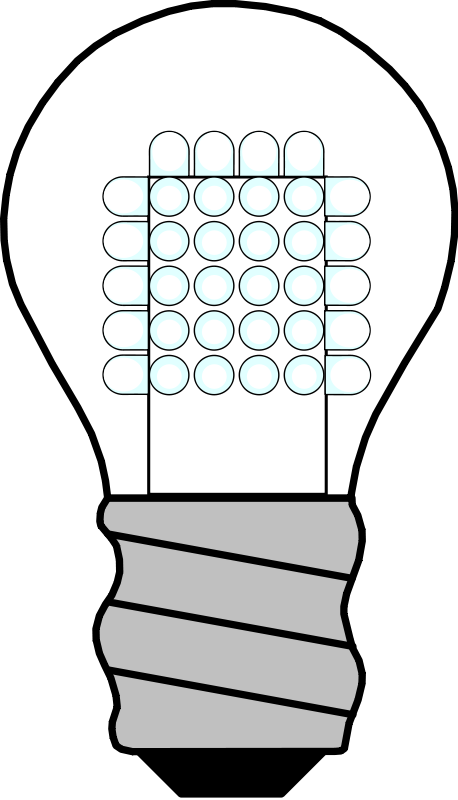
\includegraphics[scale=0.02]{imgs/bulb.png}
 \textbf{Nota} \\
 }%
{\endMakeFramed}

%Work in progress
\newenvironment{workinprogress}{%
  \def\FrameCommand{\colorbox{pink}}%
  \MakeFramed {\FrameRestore}
\lhdbend  \textbf{Work in progress} \\
 }%
{\endMakeFramed}

%Openquestion
\newenvironment{openquestion}{%
  \def\FrameCommand{\colorbox{pink}}%
  \MakeFramed {\FrameRestore}
 \textbf{Domanda aperta} \\
 }%
{\endMakeFramed}

%TODO
\newenvironment{todo}{%
  \def\FrameCommand{\colorbox{pink}}%
  \MakeFramed {\FrameRestore}
 \textbf{TODO} \\
 }%
{\endMakeFramed}

%%%%%%%%%%%%%%%%%%%%%%%%%%%%%%%%
%%%%%%%%%%%% HEADER %%%%%%%%%%%%
%%%%%%%%%%%%%%%%%%%%%%%%%%%%%%%%
\pagestyle{fancy}
% i comandi seguenti impediscono la scrittura in maiuscolo
% dei nomi dei capitoli e dei paragrafi nelle intestazioni
\renewcommand{\chaptermark}[1]{\markboth{#1}{}}
\renewcommand{\sectionmark}[1]{\markright{\thesection\ #1}}
\fancyhf{} % rimuove l'attuale contenuto dell'intestazione
% e del pi\`e di pagina
\fancyhead[LE,RO]{\bfseries\thepage}
\fancyhead[LO]{\bfseries\rightmark}
\fancyhead[RE]{\bfseries\leftmark}
\renewcommand{\headrulewidth}{0.5pt}
\renewcommand{\footrulewidth}{0pt}
\addtolength{\headheight}{0.5pt} % riserva spazio per la linea
\fancypagestyle{plain}{%
\fancyhead{} % ignora, nello stile plain, le intestazioni
\renewcommand{\headrulewidth}{0pt} % e la linea
}


%%%%%%%%%%%%%%%%%%%%%%%%%%%%%%%%
%%%%%%%%%%%% COLORS %%%%%%%%%%%%
%%%%%%%%%%%%%%%%%%%%%%%%%%%%%%%%
\definecolor{code}{gray}{0.3}


%%%%%%%%%%%%%%%%%%%%%%%%%%%%%%%%
%%%%%%%%%%%% NUMBERS %%%%%%%%%%%
%%%%%%%%%%%%%%%%%%%%%%%%%%%%%%%%
\setcounter{tocdepth}{3}
\setcounter{secnumdepth}{3}


%%%%%%%%%%%%%%%%%%%%%%%%%%%%%%%%
%%%%%%%%%%% DOC DATA %%%%%%%%%%%
%%%%%%%%%%%%%%%%%%%%%%%%%%%%%%%%
\title{Appunti di MNO}
\author{Gruppo Informatici Rampanti}
\date{ott 2010 - mag 2011}

\pdfinfo{%
  /Title    (Appunti di MNO)
  /Author   (Andrea Cimino e Lorenzo Muti)
  /Creator  (Andrea Cimino)
  /Producer (Lorenzo Muti)
  /Subject  (MNO)
  /Keywords (MNO)
}


%%%%%%%%%%%%%%%%%%%%%%%%%%%%%%%%
%%%%%%%%%%%%% UTILS %%%%%%%%%%%%
%%%%%%%%%%%%%%%%%%%%%%%%%%%%%%%%
% binary symbols
\newcommand{\modder}{\vdash _{R}}

% vertical gaps
\newcommand{\askip}{\vspace{0.5cm}}
\newcommand{\bskip}{\vspace{1.0cm}}

% various symbols
\newcommand{\qedhere}{\ensuremath{\Box}}
\newcommand{\qed}{\hfill \ensuremath{\Box}}

% substitution
\newcommand{\subst}[2]{^{#1} / _{#2}}

% denotational semantics function names
\newcommand{\bbracket}[1]{\left\llbracket #1 \right\rrbracket}

\newcommand{\aexpr}{\mathcal{A}}
\newcommand{\bexpr}{\mathcal{B}}
\newcommand{\cexpr}{\mathcal{C}}
\newcommand{\Aexpr}[1]{\mathcal{A} \bbracket{#1}}
\newcommand{\Bexpr}[1]{\mathcal{B} \bbracket{#1}}
\newcommand{\Cexpr}[1]{\mathcal{C} \bbracket{#1}}

\newcommand{\semdomset}[1]{(V_{#1})_{\bot}}

% semantic evaluations
\newcommand{\opereval}[3]{\left\langle #1, #2 \right\rangle \rightarrow #3}
\newcommand{\denaeval}[3]{\Aexpr{#1} #2 = #3}
\newcommand{\denbeval}[3]{\Bexpr{#1} #2 = #3}
\newcommand{\denceval}[3]{\Cexpr{#1} #2 = #3}

% rotated sqsubseteqs
\newcommand{\upsqsubseteq}{ $\begin{rotate}{90} $\sqsubseteq$ \end{rotate}$ }
\newcommand{\downsqsubseteq}{ $\begin{rotate}{270} $\sqsubseteq$ \end{rotate}$ }

% Space after paragraph declaration
\makeatletter
\renewcommand\paragraph{\@startsection{paragraph}{4}{\z@}%
  {-3.25ex\@plus -1ex \@minus -.2ex}%
  {1.5ex \@plus .2ex}%
  {\normalfont\normalsize\bfseries}}
\makeatother



% fast theorem and definition
\newcommand{\ftheo}[1]{\colorbox{YellowGreen}{#1}}
\newcommand{\fdefn}[1]{\colorbox{SkyBlue}{#1}}

\theoremstyle{break}
\theoremsymbol{\ensuremath{\clubsuit}}
\theoremseparator{\newline}
\newshadedtheorem{proc}[theo]{Procedura}

% bold math!
\newcommand{\bm}[1]{\mbox{\boldmath{$#1$}}}

\newcommand{\positive}[1]{\textbf{\color{green} +} #1}
\newcommand{\negative}[1]{\textbf{\color{red} -} #1}


\newtheoremlisttype{tab}%
{\begin{tabular*}{\linewidth}{@{}lrl@{\extracolsep{\fill}}r@{}}}%
{##1&##2&##3&##4\\}%
{\end{tabular*}}
\begin{document}
}
\providecommand{\outbpdocument}{\end{document}}
\else
\providecommand{\inbpdocument}{}
\providecommand{\outbpdocument}{}
\fi



\inbpdocument 

%% 5 Novembre (Bigi)
% \section{Bigi 5 nov}
\chapter{Richiami di Analisi e Ottimizzazione}
Vedremo Problemi di ottimizzazione:
 $$ f: \mathbb{R}^{n} \rightarrow \mathbb{R}, D \subseteq \mathbb{R}^{n}$$
  $$ \min \{ f(x) : x \in D \}$$
 Tovare $\overline{x} \in \mathbb{R}^{n}$ tale che
\begin{itemize}
 \item  $\overline{x} \in D$ (ammissibile)
 \item $f(\overline{x}) \leq f(x)$ per ogni $x \in D$ (punto di minimo)
\end{itemize}
Successione:
$$\{x_k\}_{k \in N} \subseteq \mathbb{R}^{n} \quad x_1,x_2,\ldots$$
Useremo la norma 2 su 
$\mathbb{R}^n$ :  $|| x ||_{2} = \sqrt{\displaystyle \sum_{i=1}^{r}x_{i}^2}$
\section{Richiami di analisi in $\mathbb{R}^{n}$}
\begin{defn}[Limite di una successione]
 $\overline{x} \in \mathbb{R}^n$ si dice limite di $\{ x_k \}_{k \in \mathbb{N}}$ 
se 
$$ \forall \varepsilon > 0 \; \exists  \overline{k} \quad \text{ t.c.} \quad  || x_k - \overline{x} ||_{2} \leq \varepsilon 
 \quad \forall k \geq \overline{k}$$
\end{defn}

\begin{example}
 $x_k = (1/k, 1/k)$ : il limite è il vettore $(0,0)$
\end{example}
Non tutte le successioni convergono
\begin{example}
 $x_k = ((1/k), (-1)^{k}) $: in questo caso il limite non esiste
\end{example}

\begin{defn}[Sottosuccessione]
 Selezione degli elementi $k_j$ tale che l'indice vada a $+\infty$.
\end{defn}
\begin{example}
Sottosuccessione $k_j = 2j-1$ ($k_j$ assume valori dispari)\\
Sottosuccessione $k_j = 2j$ ($k_j$ assume valori pari)
\end{example}
Nel caso dell'esempio, le singole sottosuccessioni definite convergono a
\begin{itemize}
 \item $(0,1)$
 \item $(0,-1)$
\end{itemize}
\begin{defn}[Punti di accumulazione della successione]
$\overline{x}$ è un punto di accumulazione di una successione
 $\{x_k\}$  se esiste una sottosequenza infinita di indici $k_j$ $ (k_1,k_2,
k_3, \ldots )$ tale che
$$\overline{x} =   \lim_{j \to +\infty}x_{k_{j}}$$

%$$ \lim_{n \to \infty}x_n	$$
\end{defn}

\begin{theo}[Bolzano-Weierstrass]
 Sia $\{x_k\}$ una successione tale che  esista una costante $M>0$ 
per cui $||x_k|| < M ~ \forall k$.\\
Allora $\{x_k\}$ ammette una sottosuccessione convergente.
\end{theo}

\begin{defn}[Insieme di vicini di $x$]
 Dato un punto $x \in \mathbb{R}^{n}$, chiamiamo
$\mathcal{N} \in \mathbb{R}^{n}$  \emph{insieme di vicini di x} se
è un insieme aperto che ccontiene $x$.
\end{defn}
Un insieme di vicini di $x$ molto utile è il seguente

\begin{defn}[Palla aperta di raggio $\varepsilon$ attorno a $x$]
Una palla aperta di raggio $\varepsilon$ attorno a $x$ \`e
definita come
$$ B(x,\varepsilon) = \{ y \; | \; ||y-x|| < \varepsilon \}$$
\end{defn}
In un piano bidimensionale abbiamo un cerchio.


\begin{defn}
 $A \subseteq \mathbb{R}^{n}$ si dice aperto se
$$\forall x \in A \quad \exists \varepsilon > 0 
   \text { t.c. }
 B(x, \varepsilon) \subseteq A
$$
\end{defn}

\begin{example}[Esempi di insiemi aperti]
  \begin{itemize}
  \item  $ ] -1, 1 [$
  \item $\mathbb{R}^{n}$
  \item $\emptyset$
  \end{itemize}
\end{example}

%% FIXME
\begin{property}
 unione di aperti è aperto
  $A_{\alpha} aperti \rightarrow \cup_{\alpha} A_{\alpha}$ è aperto
\end{property}
% {n \to \infty}

\begin{property}
\begin{itemize}
\item l'intersezione di un insieme finito di aperti è  un aperto
\item l'unione infinita di aperti è un aperto
\end{itemize}

\end{property}
L'intersezione infinita di $B(0, \frac{1}{k}) = \{0\}$ non è un aperto

\begin{defn}[Punto interno]
Sia $ A \subseteq \mathbb{R}^n$, $x$ si dice punto interno di $A$ se
$\exists \varepsilon > 0$ t.c. $B(x, \varepsilon) \subseteq A $
\end{defn}

\begin{property}
 $A$ aperto $\Longleftrightarrow ~ A=\{ \text{punti interni di  } A \}$
\end{property}

\begin{defn}[Chiuso]
$A \subseteq \mathbb{R}^{n}$ si dice \emph{chiuso} se
 $\mathbb{R}^{n} \backslash A$ (complementare) è aperto
\end{defn}

\begin{example}[Insiemi chiusi]
  \begin{itemize}
  \item $ \overline{B(x, \varepsilon) } = \{ y \in \mathbb{R}^{n} \; | \;\;  ||y-x||_{2} \leq \varepsilon \}$
  \item $\emptyset$
  \item $[-1,1]$
  \end{itemize}
\end{example}

\begin{defn}[Punto di chiusura] 
 Punto $x \in \mathbb{R}^{n}$ si dice \emph{punto di chiusura} se
 $$ \forall \varepsilon > 0: B(x, \varepsilon) \cap A \neq \emptyset $$
\end{defn}

\begin{property}
 A è chiuso $\Longleftrightarrow  A = \{ \text{punti di chiusura} \}$
\end{property}
Notazione:
$(\overline{A}, cl(A))$


\begin{property}
\begin{itemize}
 \item $A_{\alpha}$ chiusi $\Rightarrow$ $\cap_{\alpha} A_{\alpha}$ è chiuso.
  L'intersezione infinita di chiusi è un chiuso.
 \item $A_{i}$ chiusi $i=1 \ldots k \Rightarrow 
\displaystyle \bigcup_{i=1}^{k}A_{i}$ è chiuso.
L'unione finita di chiusi è un chiuso.
\end{itemize}

Ci sono per\`o degli elementi che possono essere sia aperti che chiusi e altri che non sono né aperti né chiusi \\
Gli insiemi vuoti e $\mathbb{R}^{n}$ sono sia aperti che chiusi.
\end{property}

\begin{example}[Insieme di elementi che non sono né aperti né
 chiusi]
 Prendiamo un rettangolo ed una palla (figura!)
 % FIXME aggiungere figura
$$([-1,0] \times [-1,1]) \cup B(0,1) = A$$
\begin{itemize}
\item 
   $(-1- \varepsilon, 0) \in B((-1,0),\varepsilon) \quad \forall \varepsilon$
   :  $A$ non è aperto
\item 
   $x_k = (1 - \frac{1}{k},0) \in A \quad x_k \rightarrow (1,0) 
 \notin A $: $A$ non è chiuso
\end{itemize}
\end{example}

\begin{property}
$A \subseteq \mathbb{R}^n $ è chiuso $\Longleftrightarrow
 \forall \{ x_k \} \subseteq A $ per cui $x_k  \rightarrow \overline{x}$
risulta $\overline{x} \in A $
\end{property}

\begin{defn}[Insieme limitato]
$A \subseteq \mathbb{R}^{n}$ si dice \emph{limitato}  se $\exists M > 0$ per cui
$|| x ||_{2} \leq M \; \forall x \in A $
\end{defn}

\begin{defn}[Insieme compatto]
 $A \subseteq \mathbb{R}^{n}$ si dice \emph{compatto} se A è limitato e chiuso.
\end{defn}
Gli insiemi compatti sono interessanti per il seguente motivo

\begin{theo}[Bolzano-Weirstrass]
\label{richiamibigi:bolzanow01}
 Sia $A \subseteq \mathbb{R}^{n}$ un insieme compatto.\\
 Ogni successione  $\{x_k\}_{k} \subseteq A$ ammette una sottosuccesione
 convergente.  Ossia
$$ \exists \{ x_{k_{j}}\} \subseteq A, \overline{x} \in A \text{ t.c. } x_{k_j} \rightarrow_{j \to + \infty} \overline{x}$$
\end{theo}

\subsection{Funzioni di pi\`u variabili a valori reali}%$f: \mathbb{R}^{n} \rightarrow \mathbb{R}}$

\begin{defn}[Funzione continua]
 $f$ si dice \emph{continua} in $\overline{x} \in \mathbb{R}^{n}$ se
 $$ \forall \varepsilon > 0 \quad \exists \delta > 0  \quad  \text{t.c.} \quad
\forall x \in \mathbb{R}^{n} : || x-\overline{x} ||_{2} \leq \delta  \Rightarrow | f(x) - f(\overline{x})| \leq \varepsilon $$ 
\end{defn}

\begin{property}
\label{richiamibigi:propfunzcont}
$f$ è continua in $\overline{x} \in \mathbb{R}^{n} \Longleftrightarrow
\forall \{x_k\}$ t.c. $x_k \rightarrow \overline{x}$ risulta 
$ \displaystyle \lim_{k \to +\infty}f(x_k) = f(\overline{x})$
\end{property}


\begin{example}[Esempi di funzioni continue]
  \begin{itemize}
  \item  $f(x) = || x ||_{2}$
  \item $f(x_1,x_2) = \sin(\pi x_1x_2)$
  \end{itemize}
\end{example}

\begin{defn}[Lipschitziana]
\label{def:lipschitziana}
Una funzione \emph{lipschitziana} è una funzione che ha una crescita
limitata, nel senso che il rapporto tra variazione di ordinata e
variazione di ascissa non può superare un valore fissato, detto
costante di Lipschitz. È una condizione più forte della continuità.
$$ \frac{||f(x_2) - f(x_1)||}{|| x_2 - x_1 ||} \leq L $$
\end{defn}


\begin{defn}[Estremo superiore]
Sia $(X,\leq)$ un insieme totalmente ordinato, $E\subseteq X$.
 Se esiste un elemento $y\in X$ tale che:
\begin{itemize}
\item $y$ è un maggiorante di $E$
\item se $z<y$ allora $z$ non è un maggiorante di $E$
\end{itemize}
diciamo che $y$ è \emph{estremo superiore} di $E$, in simboli
 $y=\sup E$ e diciamo che $E$ è limitato superiormente.
\end{defn}
La definizione di estremo inferiore è simmetrica.

\begin{defn}[Massimo]
Si definisce \emph{elemento massimo} di $S$  un elemento $M \in S$
 tale che
$$\forall a \in S,\ a\leq M$$
\end{defn}
La definizione di minimo è simmetrica.


\begin{theo}[Weirstrass per funzioni continue]
 Sia $A \subseteq \mathbb{R}^n$ compatto e
 $f: \mathbb{R}^{n} \rightarrow \mathbb{R}$ continua su $A$. \\
Allora $f$ ammette massimo e minimo su $A$.
\end{theo}

\begin{thproof}
Poniamo $ l = \inf \{f(x):  x \in A \} \in [ -\infty, + \infty]$.
Sicuramente esiste successione $f(x_k) \rightarrow l$ con $x_k \in A$. (per definizione di estremo inferiore). Ma
\begin{itemize}
\item Per la  (\ref{richiamibigi:bolzanow01}), $A$ compatto $\Rightarrow \exists x_{k_{j}} \rightarrow \overline{x}$

\item  Per la  (\ref{richiamibigi:propfunzcont})
$f$ continua $\Rightarrow  f(x_{k_{j}}) \rightarrow f(\overline{x})$ 
\end{itemize}
Allora, con l'unicità del limite,
 $f(\overline{x}) \Rightarrow l \neq -\infty \Rightarrow 
\min \{f(x): x \in A \}$

%  $x_k \in A $ $\{ x_k\} \subseteq A $
% $\{x_k\} \subseteq A$
% Per weirstrass
% $$x_{k_j} \rightarrow \overline{x} \in A $$
% Allora
% $$ f(\overline{x}) \leftarrow f(x_{k_j}) \rightarrow l$$
% Poiche il limite se esiste è unico
% $$f(\overline{x}) = l $$
\end{thproof}

\begin{example}
 $n = 1$  $f(t) = e^{-t}$, $A = \mathbb{R}_{+}$
 $$\inf \{ f(t): t \in A \} = 0$$ 
Ma il minimo non esiste! Quindi l'insieme non è compatto.
\end{example}

\subsection{Derivate}
Per le funzioni $f:\mathbb{R} \rightarrow \mathbb{R}$ abbiamo definito
la derivata come
$$ \lim_{t \to 0 } \frac{f(\overline{x} + t) - f(\overline{x})}{t}$$
Nel caso pi\`u generale di funzioni $f:\mathbb{R}^n \rightarrow \mathbb{R}^n$
consideriamo il punto $\overline{x}$ e l'insieme di vettori 
$$ \{ \overline{x} + tv \; | | \; t \geq 0  \} \quad  v \in \mathbb{R}^n, || v||_{2} = 1 \quad v:\text{direzione} $$

\begin{defn}[Derivata direzionale]
$f$ si dice \emph{derivabile in} $x \in \mathbb{R}^{n}$ 
\emph{nella direzione} $v$ se esiste
$$D_v f(\overline{x}) = \lim_{t \to 0 } \frac{f(\overline{x} + tv) - f(\overline{x})}{t}$$
\end{defn}

Le derivate direzionali sono una generalizzazione delle derivate
parziali, nelle quali si scelgono come vettori direzionali quelli
del tipo
$$ e_i = (0,0,0,\ldots, 0,\underbracket{1}_{\text{i-esima}},0, \ldots, \ldots, 0) $$
ecco una definizione più formale
\begin{defn}[Derivata parziale]
Si definisce derivata parziale di $f$ in $x$ rispetto alla variabile
$k-$esima $x_k$ il limite, se esiste finito
$$\frac{\partial f}{\partial x_k} (x)=\lim_{h\to 0}\frac{f(x_1,x_2,\ldots,x_k+h,\ldots,x_n)-f(x_1,x_2,\ldots,x_n)}{h}$$
\end{defn}

\begin{example}[Derivata parziale di $sin(\pi x_1 x_2)$]
\label{richiamibigi:example01}
$$f(x_1,x_2) = \sin(\pi x_1 x_2)  $$
Le 2 derivate parziali sono
$$
\frac{\partial f}{\partial x_1}(x) = \pi x_2 \cos(\pi x_1 x_2)
\qquad
\frac{\partial f}{\partial x_2}(x) = \pi x_1 \cos(\pi x_1 x_2)
$$
\end{example}

\begin{defn}[Gradiente]
$\nabla f(\overline{x}) = 
(\frac{\partial f}{\partial x_1}(\overline{x}),
\frac{\partial f}{\partial x_2}(\overline{x}),
\ldots,
\frac{\partial f}{\partial x_n}(\overline{x}))$
\`e detto \emph{gradiente} di $f$ in $\overline{x}$
\end{defn}
Informalmente, il gradiente indica la direzione di massima pendenza.\\
Nell'esempio (\ref{richiamibigi:example01}),  il vettore
$$ \nabla f(\overline{x}) = 
\begin{pmatrix}
  \pi x_2 \cos(\pi x_1 x_2) \\
\pi x_1 \cos(\pi x_1 x_2)
\end{pmatrix}
$$
i cui elementi sono le derivate parziali precedentemente calcolate,
è il \emph{gradiente di} $f$ \emph{in} $\overline{x}$.\\

%% 10 novembre
Prendiamo $ f: \mathbb{R}^{n} \rightarrow  \mathbb{R}$, $v \in \mathbb{R}^n$, $\Vert v \Vert = 1$

\begin{defn}[Two-sided derivate]
$$\dfrac{\partial f}{\partial v}(\overline{x}) = \lim_{t \to 0} \dfrac{[f(\overline{x}+t \cdot v)-f(\overline{x})]}{t}$$
\end{defn}

\begin{defn}[One-sided directional derivate]
$$f'(\overline{x}, v) = \lim_{t \to 0^{+}} \dfrac{[f(\overline{x}+t \cdot v)-f(\overline{x})]}{t}$$
Il limite invece che andare a $0$ da entrambi i lati, ci va solo da $0^+$.
\end{defn}

\begin{notes}
A volte esiste una e non l'altra.
\end{notes}

\begin{example}[Derivate della norma]
 $$f(x) = || x ||_2 = ( \displaystyle \sum_{i=1}^{n} x_i^2)^{1/2} \quad
 v \in \mathbb{R}^{n} \quad ||v||_{2} = 1 \quad, \overline{x} = 0
 $$
$$  \frac{f(\overline{x} + tv) - f(\overline{x})}{t} = \frac{f(tv)}{t} = 
\frac{( \displaystyle \sum_{i=1}^{n} t^{2}v_{i}^{2})^{1/2}}{t} = 
\frac{|t| (\displaystyle \sum_{i=1}^{n} v_i^{2})^{1/2}}{t} =sgn(t) ||v||_{2} = sgn(t) 
$$
Quindi $f'(\overline{x}, v) = 1$ mentre $\dfrac{\partial f}{\partial v}(\overline{x})$ non esiste.
\end{example}

\begin{example}[Esempi di calcolo di derivata in $\mathbb{R}^{n}$]
Prendiamo ad esempio la funzione $f$ definita nel seguente modo
\begin{equation}
\label{richiamibigi:example01}
f(x_1,x_2) =
\begin{cases}
\left(\frac{x_1^2 x_2}{x_1^4+x_2^2}\right)^2 & \text{ se } (x_1,x_2) \neq (0,0)\\
indef. & \text{ se } (x_1,x_2) = (0,0)
\end{cases}
\end{equation}

Ponendo  $x_2 = \alpha x_1^2,$  risulta
$$f(x_1, \alpha x_1^2) = \left[\alpha x_1^4 \cdot (x_1^4 + \alpha^2 x_1^4 ) \right]^2 = \left[\alpha / (1+ \alpha^2 ) \right]^2$$
% \cdots ~ \mbox{$f$ non è continua.}
% $$

\begin{openquestion}
  Perch\`e ha voluto introdurre questo $\alpha$?
  Voleva mostrare qualcosa in particolare?
\end{openquestion}

$f$ risulta non continua in $\overline{x} = (0,0)$.
Consideriamo infatti le seguenti successioni:

\begin{itemize}
\item $f(\frac{1}{k}, \frac{1}{k^2})$. Sostituendo i parametri
  in (\ref{richiamibigi:example01}) otteniamo il valore costante
  $1/4$.\\
 Per $k \to +\infty$ la successione converge a $(0,0)$ , ma risulta
 $$ \lim_{ k \to \infty} f\left(\frac{1}{k}, \frac{1}{k^2}\right) = 1/4
     \quad \neq \quad 
     ? = f(\overline{x})
 $$
\item $f(\frac{1}{k}, \frac{2}{k^2})$: discorso analogo al caso precedente.
Risulta infatti $f(\frac{1}{k}, \frac{2}{k^2}) = 4/25$, ma
 $$ \lim_{ k \to \infty} f\left(\frac{1}{k}, \frac{2}{k^2}\right) = 4/25
 \quad \neq \quad 
? = f(\overline{x})
$$
\end{itemize}

\begin{openquestion}
Perch\`e ha mostrato due esempi? Non ne bastava solo uno per
provare la non continuit\`a?
\end{openquestion}
Facciamo vedere che esistono le derivate direzionali di $f$
in $\overline{x}=(0,0)$ in tutte le direzioni. Ricordiamo
che $x$ e $v$ sono vettori e $t$ \`e uno scalare.
Poniamo $f(\overline{x}) = 0$.
$$
\begin{array}{c}
\displaystyle \frac{\partial f}{\partial v}(\overline{x})=
\displaystyle \frac{\partial f}{\partial v}((0,0))=
\displaystyle  \lim_{t \to 0}
\dfrac{f\left(\left(0,0 \right) + t\left(v_1,v_2 \right) \right) - 
\overbracket{f((0,0))}^{0}}{t} = \\
\displaystyle  \lim_{t \to 0}
 \dfrac{f \left(\left(tv_1,tv_2 \right) \right)}{t} =
\displaystyle  \lim_{t \to 0}\frac{[t^3 v_1^2 v_2 /(t^4 v_1^4 + t^2 v_2^2)]^2}{t} 
= \displaystyle \lim_{t \to 0} t v_1^{4} v_2^{2} / (t^2 v_1^4 + v_2^2)^2 
  \xrightarrow{t \to 0} 0
\end{array}
$$
\end{example}
Dall'esempio precedente abbiamo stabilito qundi che la propriet\`a:
$$ 
\varphi: \mathbb{R} \rightarrow \mathbb{R},  \qquad 
\varphi \text{ derivabile in } \overline{x}
\quad
\Longrightarrow
\quad
\varphi \text{ continua in } \overline{x}
$$
non vale in generale in $\mathbb{R}^{n}$.

\begin{notes}
Le derivate in tutte le direzioni esistono, quindi non è come nelle
equazioni ad una variabile: se $f$ è derivabile, non è 
necessariamente continua.
\end{notes}


\begin{defn}[Funzione lineare]
Una funzione $L$ è lineare se e solo se
$$
x,y \in \mathbb{R}^n  \quad  \alpha,  \beta \in \mathbb{R}
\qquad L(\alpha x + \beta y) = \alpha \cdot L(x) + \beta \cdot L(y) 
$$
ovvero:
$$
L(x) = l^T x = \sum_{i=1}^{n}l_i x_i
$$
\end{defn}

\begin{defn}[Funzione differenziabile]
$f: \mathbb{R}^n \to \mathbb{R}$ si dice \emph{differenziabile} 
in $\overline{x} \in \mathbb{R}^n$ se $\exists ~ L: \mathbb{R}^n \to \mathbb{R}$
lineare tale che
$$\forall h \in \mathbb{R}^n 
\quad 
 f(\overline{x}+h)=f(\overline{x}) + L(h) + r_{\overline{x}}(h)$$
con $r_{\overline{x}}(h)$ un resto tale che  $\dfrac{r_{\overline{x}}(h)}{\Vert h\Vert_2} \to 0 $ per  $ \Vert h\Vert_2 \to 0$
\end{defn}

\begin{openquestion}
 Mi sembra di aver capito che una funzione differenziabile
implica che tutte le derivate, da tutte le direzioni, sono
esprimibili come combinazione lineare delle derivate della
base canonica. La cosa verr\`a esplicitata nell'esercizio
(\ref{richiamibigi:exercise01})
\end{openquestion}
In altri termini, la differenza tra la funzione in un punto e la
funzione calcolata in $\overline{x}$ è approssimata da una funzione lineare.

\begin{property}
Sia $f:\mathbb{R}^n \rightarrow \mathbb{R}$

$f$ differenziabile in $\overline{x} \quad \Longrightarrow \quad f$
 continua in $\overline{x}$
\end{property}
 
\begin{notes}
(Quest'ultima proprietà è simile a quella delle funzioni a una variabile)  
\end{notes}

\begin{property}
\label{richiamibigi:diffimpliesderivatives}
Sia $f:\mathbb{R}^n \rightarrow \mathbb{R}$

$f$ differenziabile in $\overline{x} 
\quad \Longrightarrow \quad f$ ammette derivate in $\overline{x}$ in ogni
direzione $v$.
\end{property} 

\begin{thproof}
$$
\begin{array}{c}
 \dfrac{\partial f}{\partial v}(\overline{x}) = 
 \displaystyle
 \lim_{t \to 0} \dfrac{f(\overline{x}+ tv) - f(\overline{x})}{t} =
 \lim_{t \to 0} \dfrac{L(tv)+ r_{\overline{x}}(tv)}{t} =
 \lim_{t \to 0} \dfrac{tL(v)+ r_{\overline{x}}(tv)}{t} =
 L(v) + \lim_{t \to 0}  \dfrac{r_{\overline{x}}(tv)}{t} = L(v) \\ \\

\Vert tv \Vert_2 = t \Vert v \Vert_2 = t
\end{array}
$$
(Nota che $\Vert v \Vert_2 = 1$)
\end{thproof}

\begin{openquestion}
Da quello che ho capito dalle note
una volta stabilito che  \\
$f$ differenziabile in $\overline{x} 
\quad \Longrightarrow \quad f$ ammette 
derivate in $\overline{x}$ in ogni direzione $v$.
\\Si vuole avere un metodo esplicito per calcolare
la derivata direzionale. Chiedere lumi.
A occhio mi viene da dire che, una volta calcolate le derivate
parziali della base canonica, possiamo ricavare le derivate
delle direzioni facendo un semplice prodotto riga per colonna.
La condizione che deve essere rispettata \`e che $f$ deve
essere differenziabile.
\end{openquestion}

\begin{observation}[Calcolo esplicito della derivata direzionale]
Sfruttiamo le seguenti ipotesi:
$$v \in \mathbb{R}^n \qquad \Vert v \Vert_2 = 1 
    \qquad  v=\sum_{i=1}^{n}v_i  e_i 
\qquad \underbracket{f \text{ differenziabile}}_{\text{CHECKME}}
$$
calcoliamo quindi la  derivata direzionale
$$
\frac{\partial f}{\partial v}(\overline{x}) =
 L(v) =
 L \left( \sum_{i=1}^n v_i  e_i \right)
 \; \underbracket{=}_{1)}  \;
  \sum_{i=1}^n v_i \cdot L(e_i) = 
  \sum_{i=1}^n v_i \frac{\partial f}{\partial x_i}(\overline{x})  =
   \nabla f (\overline{x})^T v $$
  \begin{enumerate}
  \item $L$ è lineare
  \end{enumerate}
\end{observation}

\begin{exercise}
\label{richiamibigi:exercise01}
Esercizio per casa: studia
$$
   f(x_1, x_2)= \begin{cases}x_1^2 x_2 / (x_1^2 + x_2^2)  
    & \mbox{se } (x_1, x_2) \neq (0,0)  \\
   0 & \mbox{se } (x_1,x_2) = (0,0)\end{cases}
$$
\textbf{Svolgimento} \\
Vediamo che questa funzione non \`e differenziabile in
$\overline{x} = (0,0)$
$$
\dfrac{\partial f}{\partial v} (\overline{x})
=
\lim_{t \to 0}
\dfrac{t^{3}v_1^{2}v_2 / t^{2}(\overbracket{v_1^{2} + v_2^{2}}^{||v||_2^{2}})}{t}
=
v_1^{2}v_2
 \qquad ( \text{poich\`e } ||v||_{2}^{2} = v_1^{2} + v_2^{2} = 1)
$$
In particolare abbiamo
$$\dfrac{\partial f}{\partial x_1} (\overline{x})
=
\dfrac{\partial f}{\partial x_2} (\overline{x})
=
0
$$
Per farlo vedere, specialmente in questa fase iniziale del corso,
eplicitiamo i conti:
$$\dfrac{\partial f}{\partial x_1} (\overline{x}) =
1^{2}\cdot 0  = 0
$$ 
Nell'altro caso
$$\dfrac{\partial f}{\partial x_2} (\overline{x}) =
0^{2}\cdot 1  = 0
$$ 
ma $\dfrac{\partial f}{\partial v} (\overline{x}) \neq 0$
per ogni altra direzione. Quindi
$
\dfrac{\partial f}{\partial v} (\overline{x})
\neq
\nabla f(x)^{T}v = 0
$ \\
\begin{openquestion}
\`E vero che il motivo profondo della disuguaglianza \`e che la derivata
in ogni direzione non \`e esprimibile come combinazione
lineare delle derivate perziali sulle direzioni della base canonica?
\end{openquestion}
\end{exercise}

\begin{theo}[Differenziale totale]
\label{richiamibigi:differenzialetotale}
Sia $f:\mathbb{R}^n \to \mathbb{R}$, tale da ammettere derivate
parziali in ogni $x \in B(\overline{x},\varepsilon)$ per qualche
$\varepsilon > 0$. Allora
$$
\frac{\partial f}{\partial x_i}: B(\overline{x}, \varepsilon)
 \to \mathbb{R}  \text{  continua in  } \overline{x}
\quad  \Longrightarrow \quad f  \text{  differenziabile in  }
 \overline{x}
$$

$$f \to \frac{\partial f}{\partial x_i}(\overline{x})$$
\end{theo}

\begin{example}
Vediamo un'applicazione pratica del teorema
 (\ref{richiamibigi:differenzialetotale}) appena enunciato. 
Dalla tabella di verit\`a delle implicazioni  possiamo stabilire 
che vale la propriet\`a
$$
 (a \; \Longrightarrow \; b ) \quad
\Longleftrightarrow \quad
(\neg b \; \Longrightarrow \;  \neg a )
$$

Facciamo vedere quindi che non derivabilit\`a implica
non continuit\`a. \\
Riprendiamo l'esercizio (\ref{richiamibigi:exercise01}):
$$
\begin{array}{c}
\dfrac{\partial f}{\partial x_1}(x) =
\underbracket{D(x_1^2 x_2 / (x_1^2 + x_2^2))}_{\text{rispetto a } x_1} 
\underbracket{=}_{1)}
\dfrac{
D(x_1^2 x_2 ) (x_1^2 + x_2^2) 
-
x_1^2 x_2  D(x_1^2 + x_2^2) 
} { (x_1^2 + x_2^2)^{2}} =   \\
 \dfrac{ \cancel{2x_1 x_2^{3}}
+2x_2^{3} x_1   \cancel{ - 2x_1 x_2^{3}}
}{(x_1^{2} + x_2^{2})^{2}} 
=
\dfrac{2x_2^{3} x_1 }{(x_1^{2} + x_2^{2})^{2}} 
\end{array}
$$
\begin{enumerate}
\item Derivata del rapporto
\end{enumerate}
Ponendo $x_1 = x_2 = k$, $k \neq 0$ otteniamo
$$
\dfrac{\partial f}{\partial x_1}(x_1,x_2) =
\dfrac{2k^{4}}{(2k^{2})^{2}} = \dfrac{1}{2}$$ 

Mentre, come visto precedentemente nell'esempio
$$\dfrac{\partial f}{\partial x_1}(0,0) = 0$$
\end{example}

\begin{property}[Funzioni composte]
Sia
$f\; : \; \mathbb{R}^n \to \mathbb{R}$  differenziabile in
$ \overline{x} \in \mathbb{R}^n$,
$\Phi \; : \;  \mathbb{R} \to \mathbb{R} $ derivabile in 
$f(\overline{x}) \in \mathbb{R}^n$. \\
Allora
$\Phi \circ f:\mathbb{R}^n \to \mathbb{R}$ è differenziabile in 
$\overline{x}$ con

$$  \nabla(\Phi \circ f)(\overline{x}) = 
\Phi'(f(\overline{x})) \nabla f(\overline{x})$$
\end{property}

\begin{theo}[Valor medio]
$f:\mathbb{R}^n \to \mathbb{R}$ è differenziabile (su tutto $\mathbb{R}^n$)
con continuità (cioè $x \mapsto \nabla f(x)$ è continua)
su $\mathbb{R}^{n}$. \\
Dati $\overline{x}, h \in \mathbb{R}^n$, esiste $t \in (0,1)$ t.c.
 $$f(\overline{x}+h) = f(\overline{x}) + \nabla f(\overline{x} + th)^T h$$
\end{theo}

\begin{notes}
Notare che $x + th$ appartiene al segmento di estremi $x$ e $x+h$.
Ricordare inoltre il caso
$$  \Phi : \mathbb{R} \rightarrow \mathbb{R}\; : \;
\Phi(t_1) = \Phi(t_0) +   \Phi'(\xi)(t_1 -t_1)
\text{ per un opportuno } \xi
\in (t_1, t_0)
(t_0,t_1) 
$$
\end{notes}

\begin{defn}[Formula di Taylor del 1$^o$ Ordine]
Sia $f:\mathbb{R}^{n} \rightarrow \mathbb{R}$ differenziabile, allora la formula
di Taylor del primo ordine risulta
$$ 
f(\overline{x} + h) =
 f(\overline{x}) + \nabla f (\overline{x})^T h + r(h)
\qquad \text{ con  }\; 
\dfrac{r(h)}{||h||_{2}} \xrightarrow{ || h ||_{2} \to 0} 0$$
\end{defn}
Quest'ultima \`e una semplice riscrittura della definizione
alla luce della propriet\`a (\ref{richiamibigi:diffimpliesderivatives}) 

\begin{defn}[Iperpiano tangente]
$h = x - \overline{x}$, $h \approx 0  
\rightarrow f(x) \approx f(\overline{x})
 + \nabla f(\overline{x}^{T}(x - \overline{x})$
\\
Equazione iperpiano tangente al grafico di $f$ nel punto
 $(\overline{x}, f(\overline{x}))$
$$ \left\{ (x, f(\overline{x}) + \nabla f(\overline{x})^{T}(x-\overline{x})) 
\; | \; x \in \mathbb{R}^{n} \right\}$$
\end{defn}


\subsubsection{Derivate seconde}
$$
\begin{array}c
f:\mathbb{R}^n \to \mathbb{R} ~ \mbox{differenziabile}\\
x \to \dfrac{\partial f}{\partial v}(x) \qquad \dfrac{\partial f}{\partial v}: \mathbb{R}^n \to \mathbb{R}\\
\overline{x} \in \mathbb{R}^n, \quad v \in \mathbb{R}^n, \quad \Vert v \Vert_2 = 1, \quad w \in \mathbb{R}^n, \quad \Vert w \Vert_2 = 1\\
\dfrac{\partial}{\partial w}\left(\dfrac{\partial f}{\partial v} \right)(\overline{x}) = \lim_{t \to o}\dfrac{\frac{\partial f}{\partial v}(\overline{x} + tw)-\frac{\partial f}{\partial v}(\overline{x})}{t}\\
w = e_1, \quad v = e_j\\
\dfrac{\partial}{\partial x_1}\left(\dfrac{\partial f}{\partial x_2}\right) \underbrace{\longrightarrow}_{\mbox{si scrive}} \dfrac{\partial^2 f}{\partial x_1 \partial x_2}
\end{array}
$$  

Esercizio: $f(x_1, x_2)= sin(\pi x_1 x_2)$ calcolare le 4 derivate parziali.

\subsection{Funzioni  di pi\`u variabili a valori vettoriali}%$\mathbb{R}^{n} \rightarrow  \mathbb{R}^{n}$}
%% 12 Novembre
\begin{defn}[Matrice Jacobiana]
$F: \mathbb{R}^{n} \rightarrow \mathbb{R}^{n} \quad
F=(f_1,\ldots, f_n)$ \\
Matrice dei gradienti: righe sono i gradienti.
$$ J_{F}(x) =
\begin{pmatrix}
\nabla f_1(x)^{T} \\
 \nabla f_2(x)^{T} \\
 \ldots \\
\nabla f_n(x)^{T} 
\end{pmatrix} =
\begin{pmatrix}
\frac{{\partial} f_1(x)}{{\partial}(x_1)}(x) & \ldots &  \frac{{\partial} f_1(x)}{{\partial}(x_n)}(x)\\
 \ldots & \ldots & \ldots \\
\frac{{\partial} f_n(x)}{{\partial}(x_1)}(x) & \ldots &  \frac{{\partial} f_n(x)}{{\partial}(x_n)}(x)
% \frac{{\partial} f_n(x)}{{\partial}(x_1)}(x} ....  \frac{{\partial} f_n(x)}{{\partial}(x_n(}(x}
\end{pmatrix}
$$
\end{defn}
Il determinante della matrice Jacobiana \`e detto Jacobiano.

\subsection{Derivate di ordine superiore}
$f$ differenziabile su $\mathbb{R}^{n} 
\quad 
\Rightarrow
\quad 
\exists
\dfrac{\partial f }{\partial v}(x)
$
per ogni $x \in \mathbb{R}^{n}$, $v\in \mathbb{R}^{n}$ con 
$||v||_2 =1$ . \\
$\dfrac{\partial f }{\partial v}:
\mathbb{R}^{n} \rightarrow \mathbb{R}$ \`e una funzione
$\rightarrow$ ammette derivate nelle varie direzioni? \\
Limitiamoci alle derivate parziali: $w=e_i, v=e_j
\quad \rightarrow \quad
\dfrac{\partial}{\partial x_j} \rightsquigarrow
\dfrac{\partial^{2}f}{\partial x_i \partial x_j}
\quad
i=j \rightsquigarrow \dfrac{\partial^{2}f}{\partial x_i^{2}}
$

Funzioni  $\mathbb{R}^{n} \rightarrow  \mathbb{R}$ differenziabile:
$$\frac{{\partial} f}{{\partial}(x_j)}: \mathbb{R}^n \rightarrow \mathbb{R}$$
%%FIXME
\begin{example}
Definiamo $f$ come $ f(x_1,x_2) = \sin(\pi x_1 x_2)$
$$
\begin{array}{l}
\frac{{\partial}} {{\partial}(x_1)}f(x) = \pi x_2\cos(\pi x_1 x_2) \\
\frac{{\partial}} {{\partial}(x_2)}f(x) = \pi x_1\cos(\pi x_1 x_2)  \\

\frac{{\partial}^2 f} {{\partial} x_2 {\partial} x_1}(x) = \pi 
\cos(\pi x_1 x_2) - \pi^2 x_2 x_1 \sin(\pi x_1 x_2)       \\
\frac{{\partial}^2 f} {{\partial} x_1 {\partial} x_2}(x) 
= \pi \cos(\pi x_1 x_2) - \pi^2 x_1 x_2 \sin(\pi x_1 x_2) \\
\end{array}
$$
Le due derivate parziali sono uguali.
Scambiando l'ordine di derivazione abbiamo ottenuto lo stesso
risultato: non è un caso, deriva dal seguente teorema.
\end{example}
\begin{theo}[Schwarz/inversione ordine di derivazione]
\label{th:schwarz}
 Sia $f: \mathbb{R}^n \rightarrow \mathbb{R}$ tale che per ogni $i,j = 1\ldots n$
tali che
$\frac{{\partial}^2 f}{{\partial} x_j {\partial} x_i} \; ,\; \frac{{\partial}^2 f}{{\partial} x_i {\partial} x_j}$
esistano in $B(\overline{x}, \varepsilon)$ per $\overline{x} \in \mathbb{R}^n, \varepsilon > 0$ e siano continue in $\overline{x}$.
Allora:
$$\frac{{\partial}^2 f}{{\partial} x_j {\partial} x_i} =  \frac{{\partial}^2 f}{{\partial} x_i {\partial} x_j}$$
\end{theo}
\begin{defn}[Matrice Hessiana di $f$ in $f: \mathbb{R}^n \rightarrow \mathbb{R}$ in $\overline{x} \in \mathbb{R}^n$]
$$ \nabla^2 f(\overline{x}) = \left\{ 
 \frac{{\partial}^2 f}{{\partial} x_i {\partial} x_j}
  \right\}_{\substack{i=1 \ldots n \\j=1\ldots n}} = 
\begin{pmatrix}
\dfrac{{\partial}^2 f}{{\partial} x_1^2}(\overline{x}) & 
\dfrac{{\partial}^2 f}{{\partial} x_1 \partial x_2}(\overline{x}) & \ldots &
   \dfrac{{\partial}^2 f}{{\partial} x_1{\partial} x_n }(\overline{x}) \\
 \vdots   & \vdots  & \vdots & \vdots   \\
 \vdots   & \vdots  & \vdots  & \vdots   \\
\dfrac{{\partial}^2 f}{{\partial} x_n{\partial} x_1 }(\overline{x})
 & \ldots & \ldots &  \dfrac{{\partial}^2 f}{{\partial} x_n{\partial} x_n }(\overline{x})
\end{pmatrix}
$$
\end{defn}
Differenziabile due volte
$\frac{{\partial}^2 f}{{\partial} x_i {\partial} x_j}(x)$ esista per ogni $x \in \mathbb{R}^{n}$
e 
$\frac{{\partial}^2 f}{{\partial} x_i {\partial} x_j}: \mathbb{R}^n \rightarrow \mathbb{R}  $
sia continua su $\mathbb{R}^n$.
Questa è una matrice \emph{simmetrica}

\begin{defn}[Formula di Taylor con resto]
 $$f(\overline{\mathbf{x}}+\mathbf{h}) = f(\overline{\mathbf{x}}) +
 \nabla f(\overline{\mathbf{x}})^T\mathbf{h} + 
 \frac{1}{2}  \mathbf{h}^T \nabla^{2} f(\overline{\mathbf{x}} +
 t  \mathbf{h}) \mathbf{h}
\qquad
\text{con } t \in (0,1) \text{ opportuno}
$$
\end{defn}

\begin{defn}[Formula di Taylor secondo ordine]
 $$f(\overline{\mathbf{x}}+\mathbf{h}) = 
f(\overline{\mathbf{x}}) +
 \nabla f(\overline{\mathbf{x}})^T\mathbf{h} + 
 \frac{1}{2} 
\underbracket{ \mathbf{h}^T \nabla^{2} f(\overline{\mathbf{x}}) \mathbf{h}}_{}
+ r_{\overline{x}}(h)
\qquad
\text{con } \dfrac{r_{\overline{\mathbf{x}}}(\mathbf{h})}{||\mathbf{h}||_{2}^{2}}
\xrightarrow{||\mathbf{h}||_{2} \to 0} 0
$$

$$\mathbf{h}^{T} \nabla^{2} f(\overline{\mathbf{x}}) \mathbf{h} =
 \displaystyle \sum_{i=1}^{n} \displaystyle \sum_{j=1}^{n}
 = \frac{{\partial}^2 f}
{{\partial} x_i {\partial} x_j}
(\overline{\mathbf{x}}) h_i h_j$$
\end{defn}
Questa formula è interssante quando $h$ è piccolo, infatti
$$ 
\mathbf{h} = \mathbf{x} - \overline{\mathbf{x}} \approx 0
\; : \;
f(\mathbf{x}) \approx
\underbracket{ f(\overline{\mathbf{x}}) + \nabla f(\overline{\mathbf{x}})^{T} (\mathbf{x}-\overline{\mathbf{x}}) + 
 \underbracket{\frac{1}{2}(\mathbf{x}- \overline{\mathbf{x}})^{T}\nabla^{2} f(\overline{\mathbf{x}})(\mathbf{x}-\overline{\mathbf{x}})}_{\text{funzione non lineare}}}_{\text{approssimazione quadratica di} f  \text{ vicino a } \mathbf{x}} $$

Funzioni alle quali saremo molto interessanti sono le funzioni quadratiche
\begin{defn}[Funzione Quadratica]
Siano $ Q \in \mathbb{R}^{n \times n}, b \in \mathbb{R}^{n}, c \in \mathbb{R} $.
La funzione: $f: \mathbb{R}^{n} \rightarrow \mathbb{R}$ \`e detta
\emph{funzione quadratica} se 
 $$ 
f(x) =  \frac{1}{2} x^{T} Q x + b^{T}x + c 
=
\frac{1}{2} 
 \displaystyle \sum_{k=1}^{n} \displaystyle \sum_{l=1}^{n}
q_{kl} x_{k}x_{l} + \displaystyle \sum_{k=1}^{n} b_k x_k + c
$$
\end{defn}

\begin{notes}
Una forma quadratica \`e una funzione quadratica in cui
sono presenti solo i termini di secondo grado, ossia
$$f(x) =  \frac{1}{2} x^{T} Q x $$
\end{notes}
et{=}_{\text{simmetrica}}
\label{obs:gradiente-hessiana-funzione-quadratica}
Cosa accade se $Q$ \`e simmetrica in una funzione lineare?
Valgono le seguenti propriet\`a:
\begin{enumerate}
\item (Gradiente): $\nabla f(x) = Qx + b$
\item(Matrice Hessiana): $\nabla^{2}f(x) = Q$
\end{enumerate}
 % : $q_{kl}$ : $q_{kl} \rightsquigarrow (q_{kl} + q_{lk})/2$
% Si potrebbe pensare che questa  matrice $Q$ sia simmetrica 
% Facendo i conti:\\ 
% Gradiente di $f(x) = Qx + b$\\
% Matrice Hessiana: $Q$\\
Dimostriamo 1. Vediamo cosa vale la derivata parziale in una generica
componente $j$
$$
\begin{array}{c}
\dfrac{\partial f}{\partial x_j}(x) =
\dfrac{1}{2}
\left[\displaystyle \sum_{l=1}^{n} q_{jl}x_l 
+
\sum_{k=1}^{n} q_{kj}x_k
\right] + b_j \underbracket{=}_{\text{simmetrica}}
\dfrac{1}{2}
\left[\displaystyle \sum_{l=1}^{n} q_{lj}x_l 
+
\sum_{k=1}^{n} q_{kj}x_k
\right] + b_j = \\
\displaystyle \sum_{l=1}^{n} q_{jl}x_l + b_j =
(Qx)_j + b_j  \qquad \Longrightarrow \qquad 
\nabla f(x) = Qx + b
\end{array}
$$
Discorso analogo per il punto 2.
$$
\dfrac{\partial f}{\partial x_i \partial x_j}(x) 
= 
\dfrac{\partial f}{\partial x_i}
\left(\dfrac{\partial f}{\partial x_j}(x) 
\right)
=
\dfrac{\partial f}{\partial x_i}
\left(
\displaystyle \sum_{l=1}^{n} q_{jl} x_{l} + b_j 
\right) = q_{ji} = q_{ij}
\qquad \Longrightarrow \qquad \nabla^{2}f(x) = Q
$$
\end{observation}

\begin{exercise}
Per esercizio :
trovare l'approssimazione di Taylor del secondo
ordine di
 $f(x_1,x_2) = - x_1^4 -x_2^2$ centrata in $\overline{x} = (0, 2/5)$
 \\
\textbf{Svolgimento}
$$
\nabla f(x) = 
\begin{pmatrix}
  -4 x_1^{3} \\
  -2 x_2
\end{pmatrix}
\qquad
\nabla^{2} f(x) = 
\begin{pmatrix}
  -12 x_1^{2} & 0 \\
  0 & -2
\end{pmatrix}
$$

$$
\overline{x} = (0, 2/5)
\qquad
\nabla f(\overline{x}) = 
\begin{pmatrix}
   0  \\
  -4/5
\end{pmatrix}
\qquad
\nabla^{2} f(\overline{x}) = 
\begin{pmatrix}
  0 & 0 \\
  0 & -2
\end{pmatrix}
$$

$$
\begin{array}{l}
f(\overline{x} +h) = f(\overline{x}) +
  \nabla f(\overline{x})^{T}(x- \overline{x})
  + \dfrac{1}{2}( x - \overline{x})^{T}
   \nabla^{2} f(\overline{x}) (x - \overline{x}) = \\
-\dfrac{4}{25} - \dfrac{4}{5} (x_2 + \dfrac{2}{5}) 
   - 2(x_2 + \dfrac{2}{5}x)^{2} = \\
-\dfrac{12}{25} -\dfrac{4}{5} x^{2} - 2x_2^{2} - 
   \dfrac{8}{25} - \dfrac{8}{5} x^{2} = \\
   \dfrac{20}{25} - \dfrac{12}{5} x_2 - 2x_2^{2} 
\end{array}
$$

\begin{todo}
 Magari mettere un bel grafico 3d per evidenziare
il comportamento di Taylor. 
\end{todo}
\end{exercise}

\chapter{Ottimizzazione: regione ammissibile e condizioni di ottimalità}
\label{chap:ottimizzazioni-definizioni}
\begin{todo}
Dare un nome pi\`u sensato al capitolo ed alle sezioni.
\end{todo}
$ f: \mathbb{R}^n \rightarrow \mathbb{R}, D \subseteq \mathbb{R}^n$\\
$$\text{(P)} \qquad
\min\{ f(x)\; : \; x \in D \}
$$

Problema: trovare $\overline{x} \in \mathbb{R}^n $ tale che:

\begin{itemize}
 \item $\overline{x} \in D$
 \item $f(\overline{x}) \leq f(x) \; \forall x \in D$
\end{itemize}

\paragraph{Classificazione della regione ammissibile}
$$
\left\{
\begin{array}{ll}
 D = \mathbb{R}^{n} &      \text{ Ottimizzazione  non vincolata } \\
 D \subset \mathbb{R}^n & \text{ Ottimizzazione  vincolata } 
\end{array}
\right.
$$
%Ottimizzazione sul continuo e sul discreto.

\paragraph{Classificazione della funzione obiettivo}
$$f \text{ obiettivo}: \left\{
\begin{array}{l}
 \text{lineare} \\
 \text{non lineare}
\end{array}
\right.
$$
\begin{defn}[Punto di minimo globale]
$\overline{x} \in \mathbb{R}$ si dice 
\emph{punto di minimo globale} di (P) se
\begin{itemize}
\item $x \in D$
\item $f(\overline{x}) \leq f(x) \quad
\forall x \in D$
\end{itemize}
\end{defn}
In questo caso $f(\overline{x})$ si dice
\emph{valore ottimo} di (P)
\begin{observation}
 Punto di minimo e inf non sono la stessa cosa! \\

 Ad esempio $f(x) = e^{-x}$ ha estremo inferiore ma 
non ha minimo.Quindi possiamo afferemare che il valore
ottimo esiste (inteso come $inf\{f(x)\; : \; x \in D \}$),
ma non esiste alcun cun punti di minimo. \\
Prendiamo invece la funzione
$f(x) = -x^{2}$: il valore ottimo non esiste in quanto
$f(x) \rightarrow -\infty$.
\end{observation}
\begin{figure}[h]
  \centerline{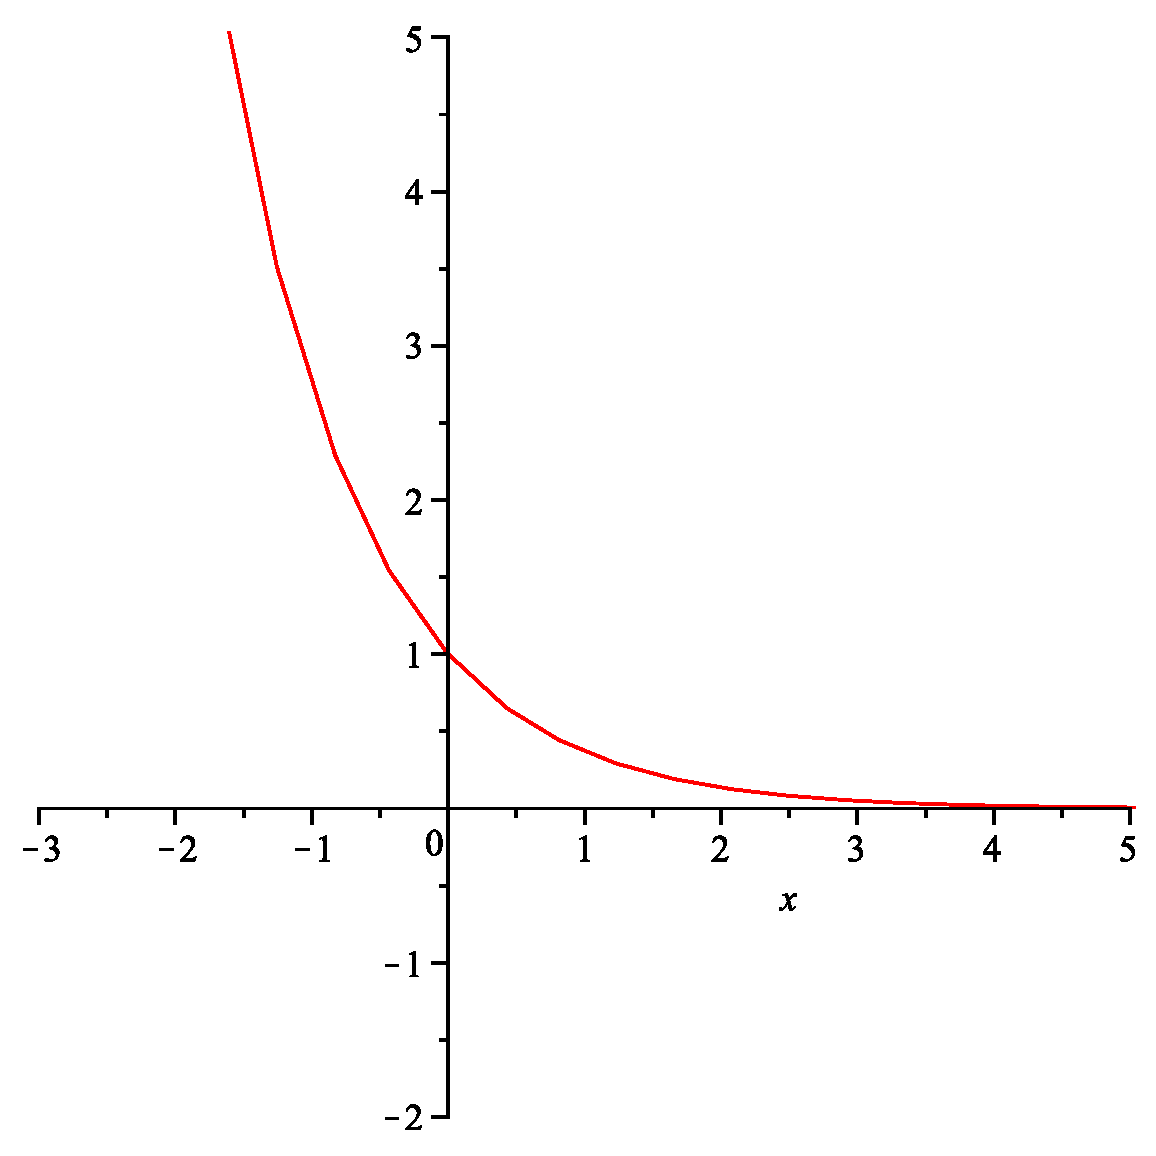
\includegraphics[scale=0.3]{imgs/fun01.pdf}}
  \label{fig:theFig}
  \caption{$f(x) = e^{-x}$}
\end{figure}

\begin{defn}[Punto di minimo locale]
 Un $\overline{x}$ si dice punto di minimo locale se
\begin{itemize}
 \item   $\overline{x} \in D$
 \item  $ \exists \varepsilon >0  \; | \; f(\overline{x}) \leq f(x) \; \forall x \in D \cap B(\overline{x}, \varepsilon)$
\end{itemize}
\end{defn}

\begin{figure}[h]
  \centerline{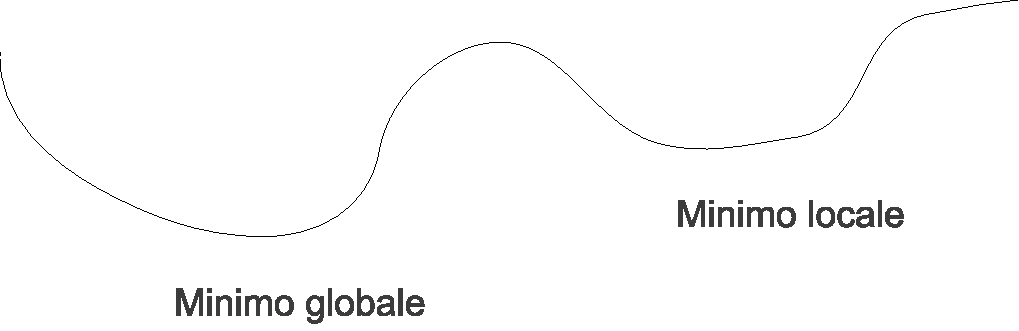
\includegraphics[scale=0.4]{imgs/img01.pdf}}
  \label{fig:theFi2}
  \caption{Minimo locale e globale}
\end{figure}

\begin{figure}[h]
  \centerline{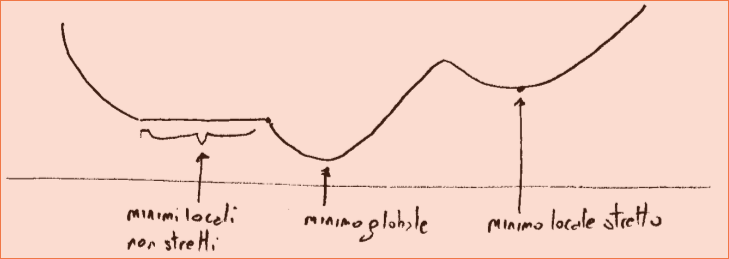
\includegraphics[scale=0.4]{imgs/img02.jpg}}
  \label{fig:theFi2}
  \caption{Minimo locale e globale}
\end{figure}

\begin{defn}[Punto di minimo locale stretto]
 Un $\overline{x}$ si dice punto di minimo locale stretto
di (P) se 
\begin{itemize}
 \item   $\overline{x} \in D$
 \item  $ \exists \varepsilon >0  \; | \; f(\overline{x}) < f(x) \quad  \forall x 
\in D \cap B(\overline{x}, \varepsilon), x \neq \overline{x}$
\end{itemize}
\end{defn}
Cioè il minimo è unico nell'intevallo selezionato.
\begin{defn}[Funzione convessa]
 Una $f: \mathbb{R}^n \rightarrow \mathbb{R}$ si dice \emph{convessa} se 
\begin{equation}
\label{richiamibigi:funzioneconvessa}
\forall x,y \in \mathbb{R}^{n}, \forall \lambda \in [0,1]
\qquad
f(\underbracket{\lambda x +(1-\lambda)y}_{\text{segmento } [x,y] \subseteq  \mathbb{R}^{n}}) \leq 
\underbracket{\lambda f(x) + (1-\lambda)f(y)}_{
\text{segmento } [f(x),f(y)] \subseteq \mathbb{R}
} 
\end{equation}
\end{defn}

\begin{defn}[Funzione concava]
 Una $f: \mathbb{R}^n \rightarrow \mathbb{R}$ si dice \emph{concava} 
 se la funzione $-f$ è convessa.
\end{defn}
\begin{figure}[!h]
  \centerline{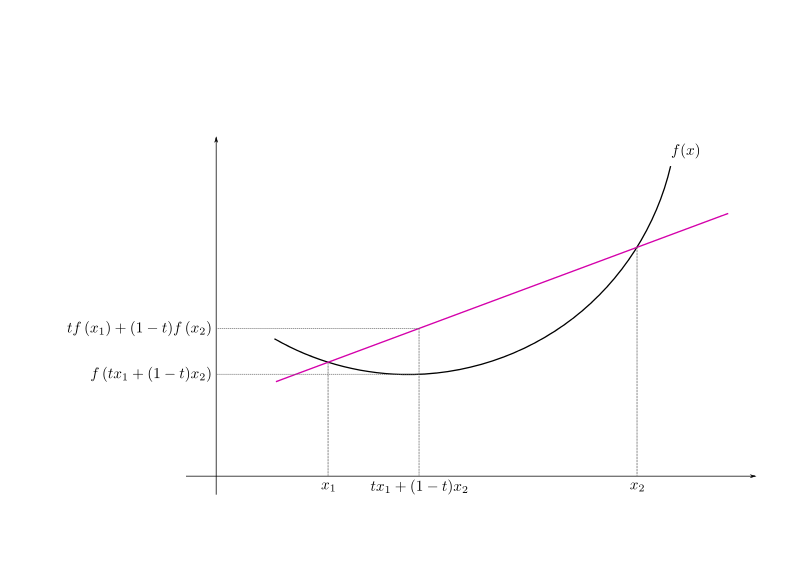
\includegraphics[scale=0.6]{imgs/img03.png}}
  \label{fig:theFi2}
  \caption{Funzione convessa}
\end{figure}

Si parla di \emph{funzioni strettamente convesse (concave)} se 
nella (\ref{richiamibigi:funzioneconvessa}) al posto
 di $\leq$ sostituiamo $<$ (simmetrico nel caso convesso).

 \begin{observation}
  $$ f \text{ \`e convessa } \; \Longleftrightarrow \;
f\left(\displaystyle \sum_{i=1}^{k} \lambda_i x_i \right) \leq 
\displaystyle \sum_{i=1}^{k} \lambda_i f(x_i)
\qquad
\forall x_1, \ldots, x_k \in \mathbb{R}^{n}, \forall \lambda_i \geq 0
\text{ con }  \displaystyle \sum_{i=1}^{k} \lambda_i = 1
$$
 \end{observation}

\begin{theo}[Locale $\equiv$ globale]
 Sia $f: \mathbb{R}^n \rightarrow \mathbb{R}$ convessa,
 $D \subseteq \mathbb{R}^n$ convesso. Allora ogni punto di minimo
 locale di (P) \`e anche un punto di minimo globale.
\end{theo}

Cioè nei problemi di ottimizzazione, se la regione ammissible è convessa,
e la funzione obiettivo \`e convessa, non c'\`e distinzione fra minimo locale e 
minimo globale.
\begin{thproof}

 Sia $\overline{x} \in D$ un minimo locale. Supponiamo, per assurdo,
che non sia un punto di minimo globale. Allora $\exists \hat{x}$ tale 
che $f(\hat{x}) < f(\overline{x})$. \\
Consideriamo il punto $x_{\lambda} = \lambda x + (1-\lambda)\hat{x}$
con $\lambda \in [0,1],  x_{\lambda} \in D$\\
Quanto vale la funzione in $x_{\lambda}$?
 $$f(x_{\lambda}) \underbracket{\leq}_{\text{convessit\`a}}  \lambda f(x) +
 (1-\lambda)f(\overline{x}) < \lambda f(\overline{x})
 + (1-\lambda) f(\overline{x})
 = f(\overline{x})$$
 $$ x_{\lambda} \xrightarrow{\lambda \rightarrow 0} \overline{x} \quad
  \forall \epsilon  \exists  \overline{\lambda} \in [0,1] \quad 
 \text{ t.c. }  \quad x_{\overline{\lambda}} \in  B(\overline{x}, \varepsilon)$$
ed inoltre
$$ f(x_{\overline{\lambda}}) < f(\overline{x})$$
Quindi $\overline{x}$ non \`e un minimo locale (contraddizione)
\end{thproof}

\begin{defn}[Insieme convesso]
 $D \subseteq \mathbb{R}^{n}$ si dice \emph{convesso} se 
$\forall x,y \in D \; \forall \lambda \in [0,1]$:
$$ \underbracket{\lambda x + (1-\lambda)y}_{\text{segmento }  [x,y] \subseteq \mathbb{R}^{n}}\in D $$
\end{defn}

\begin{observation}
 Sono insiemi convessi
 \begin{itemize}
 \item $\mathbb{R}^{n}$
 \item $\emptyset$
 \end{itemize}
\end{observation}

\begin{figure}
  \centering
  \subfloat[Insieme convesso]{\label{fig:convexset}
    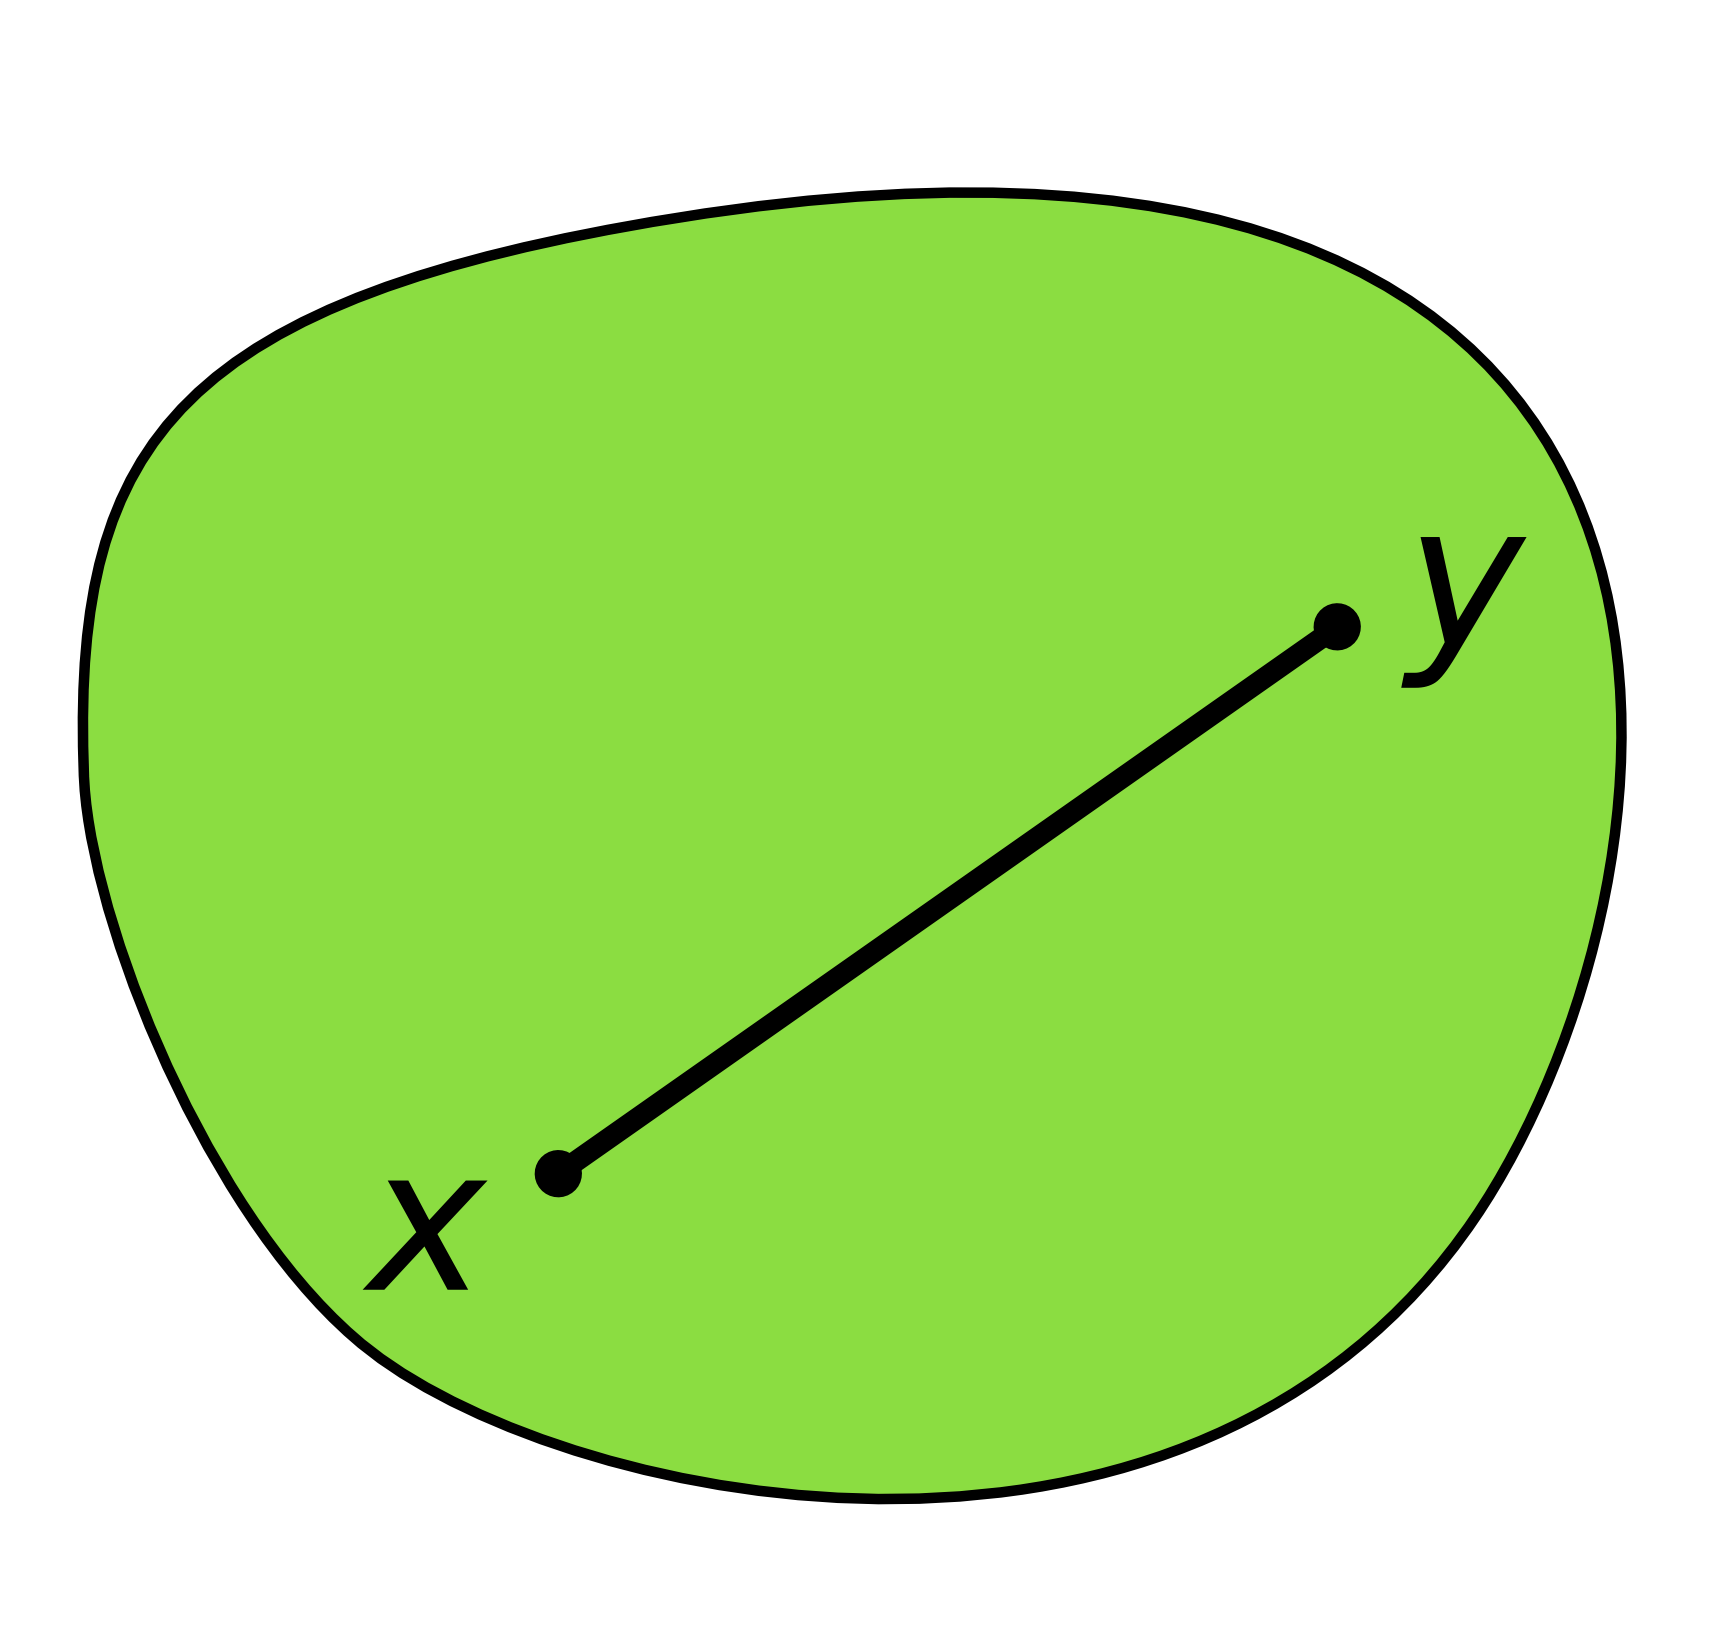
\includegraphics[width=0.25\textwidth]{imgs/img04.png}}                
  \subfloat[Insieme non convesso]{\label{fig:nonconvexset}
    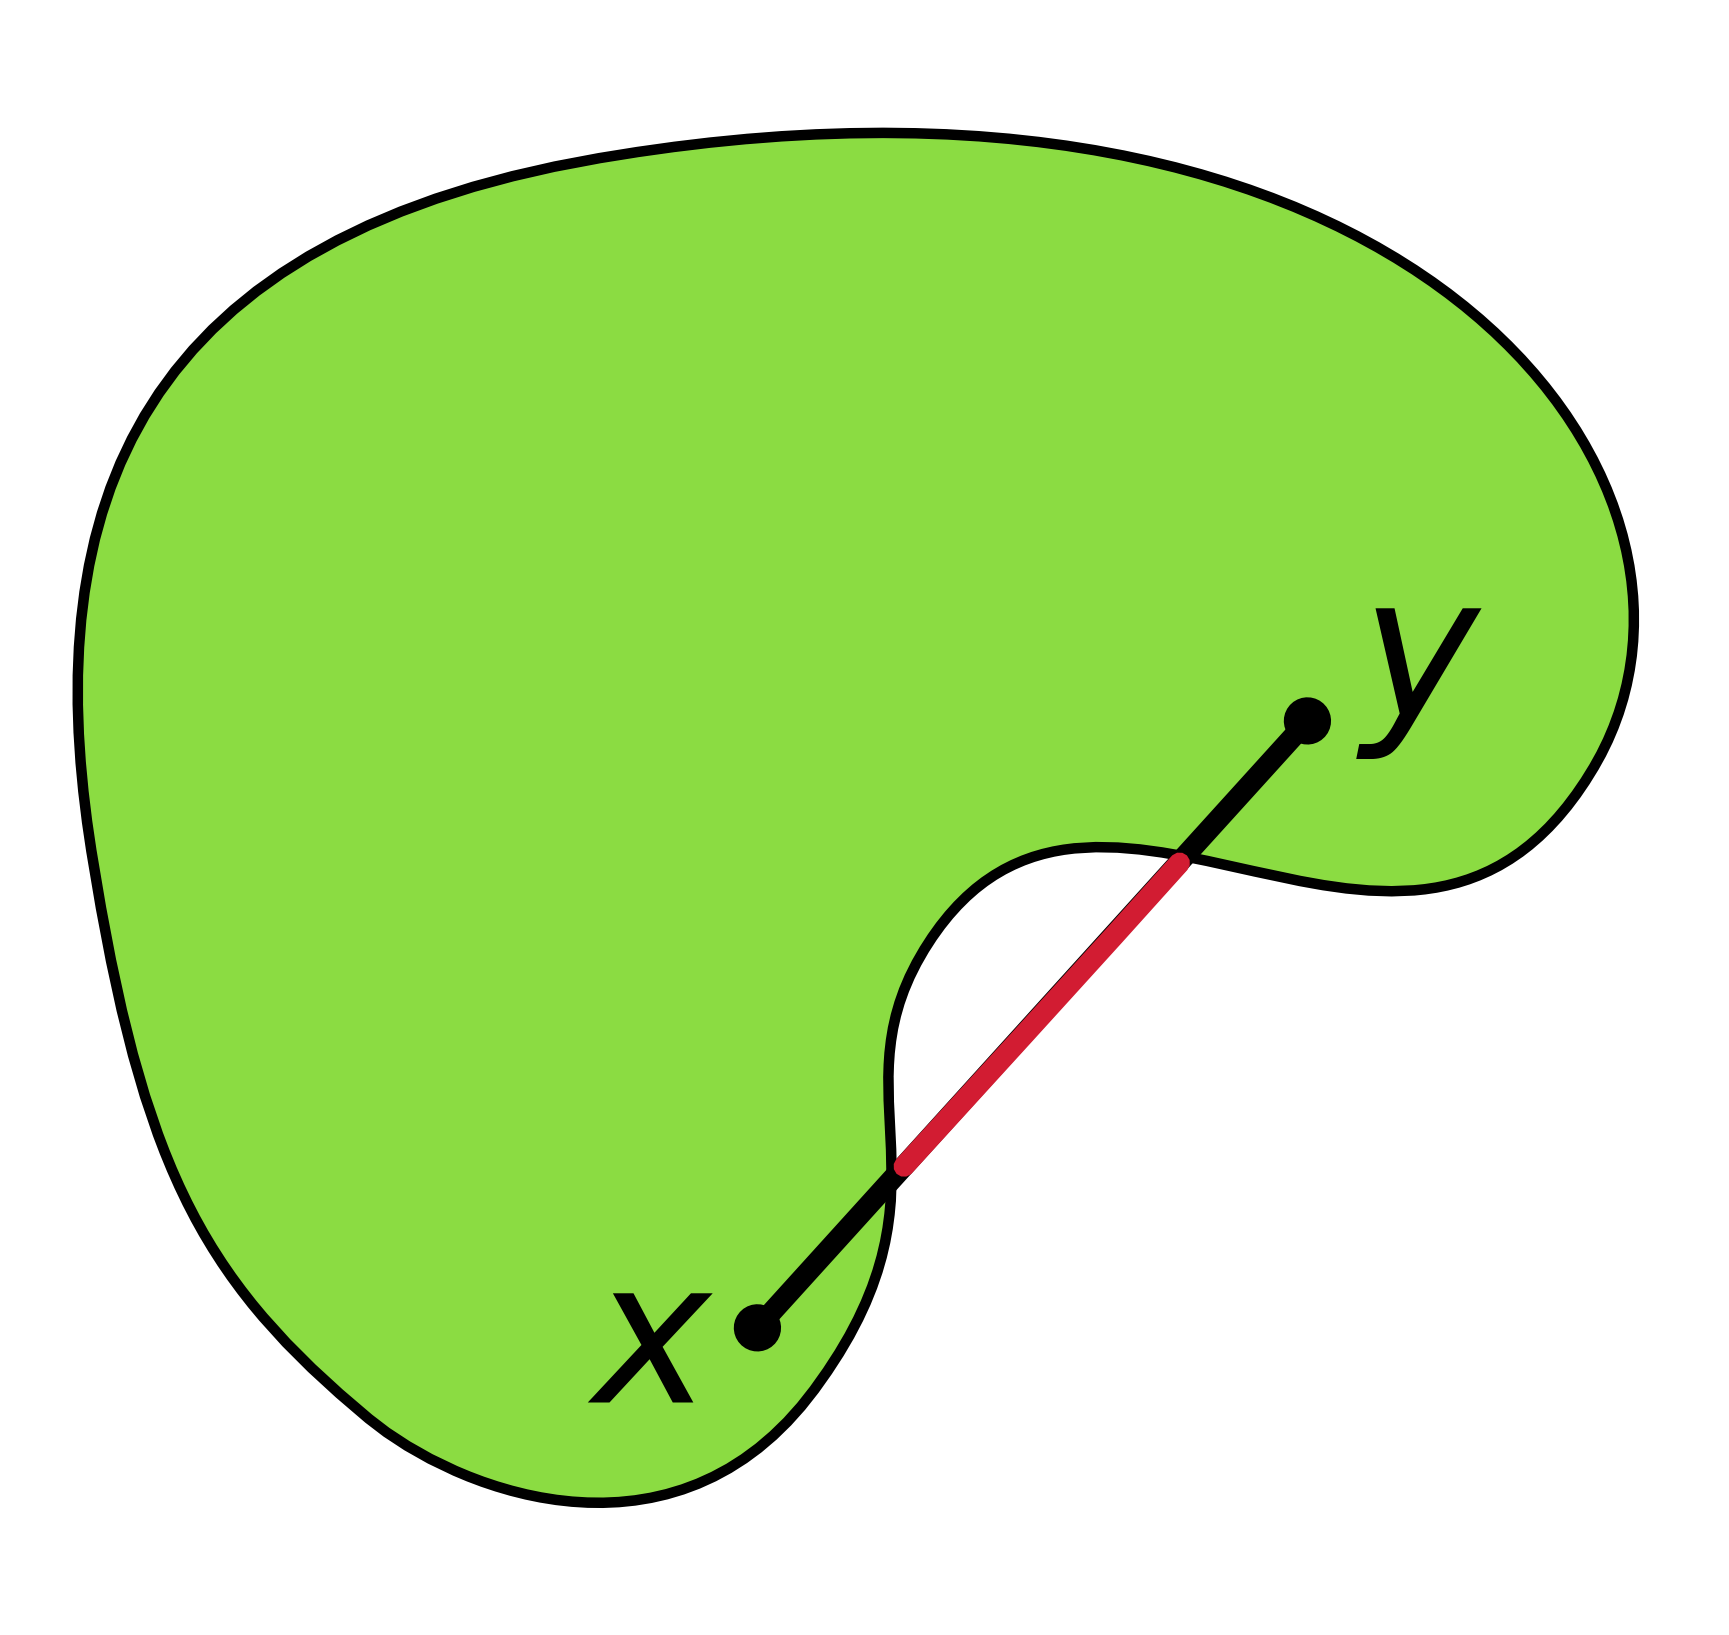
\includegraphics[width=0.25\textwidth]{imgs/img05.png}}
  \caption{Insiemi convessi e non convessi in $\mathbb{R}^2$}
  \label{fig:convexsets}
\end{figure}

\subsection{Risultati importanti su insiemi convessi
e funzione convesse}
\begin{theo}
 Sia $f: \mathbb{R}^n \rightarrow \mathbb{R}$ strettamente convessa,
$D \subseteq \mathbb{R}^n$ convesso. \\ Se (P) ammette un punto di
minimo, allora è l'unico punto di minimo.
\end{theo}

\begin{thproof}
 Sia $\overline{x} \in D$ minimo (globale $\equiv$ locale) di 
(P) e supponiamo esista $\hat{x} \in D$, $\hat{x} \neq \overline{x}$
 tale che $f(\hat{x}) = f(\overline{x})$. Sia $\lambda \in [0,1]
$ : $\lambda \hat{x} + (1-\lambda) \overline{x} \in D$
 (convessit\`a di D) e 
$$ f(\lambda \hat{x} + (1-\lambda)\overline{x}) < 
 \lambda f(\hat{x}) + (1-\lambda) f(\overline{x}) = 
 \lambda f(\overline{x}) + (1-\lambda)f(\overline{x}) =
  f(\overline{x})$$
  Quindi $\overline{x}$ non \`e un minimo 
 (globale $\equiv$ locale): contraddizione!
 \end{thproof}

\begin{notes}
 Ricordiamo che nel caso $D=\mathbb{R}^{n}$, $D$ è convesso, quindi abbiamo
automaticamente le proprietà sopra citate.
\end{notes}

\begin{notes}
Ricordiamo inoltre che i poliedri sono un insieme convesso, anche le
funzioni lineari, quindi nella programmazione lineare vale il il primo
teorema.
\end{notes}

\begin{property}
 $f$ convessa $\quad \Longrightarrow \quad f $ continua su
$\mathbb{R}^{n} $
\end{property}

\begin{property}
Sia $f: \mathbb{R}^{n} \rightarrow \mathbb{R}$.  Se $f$ è 
convessa, allora l'insieme di sottolivello
$$ C_{\alpha} = \{  x \in \mathbb{R}^{n} \; | \;  f(x) \leq \alpha \}$$
è convesso per ogni valore di $\alpha$
\end{property}

\begin{thproof}
Sia $C_\alpha \neq \emptyset$ e siano $x,y \in C_{\alpha}$. 
Allora $\forall \lambda \in [0,1]$ risulta
$$ f(\lambda x + (1-\lambda)y) \leq
 \lambda f(x) + (1-\lambda) f(y) \leq \lambda \alpha
 + (1-\lambda) \alpha = \alpha$$
da cui $\lambda + (1-\lambda)y \in C_{\alpha}$
\end{thproof}

\begin{observation} Per vedere che quest'ultima proprietà vale solo in un
senso, basta prendere la funzione $ x^{3}$, che non è convessa. I
sottolovelli sono tutti insiemi convessi.
 $$ C_{\alpha} = (-\infty, \sqrt[3]{\alpha})$$
\end{observation}

\begin{property}
  Siano  $f_i: \mathbb{R}^{n} \rightarrow \mathbb{R} $ una famiglia di
funzione convesse,  $k \in \mathbb{N}$  finito. Allora
  \begin{enumerate}
  \item $ \displaystyle \sum_{i=1}^{k} f_i $ è convessa
  \item $ \displaystyle \sup_{i \in I} f_i $ è convessa
  \end{enumerate}
\end{property}

\begin{thproof}
  \begin{enumerate}
  \item Ovvio: basta applicare la definizione ad ogni $f_i$ e
 sommare membro a membro
 \item
Nel caso $I$ sia finito allora
 $$(\sup f_i) = (\lambda x + (1-\lambda) y= 
 f_k (\lambda x + (1-\lambda)y) \leq f_k(x) + (1-\lambda) f_k(y)
 \leq \lambda (\sup f_i)(x) + (1-\lambda) (\sup f_i) (y)$$
per un $k$ opportuno
  \end{enumerate}
\end{thproof}

\begin{theo}
\label{richiamibigi:theo01}
 Sia $f$ differenziabile (su $\mathbb{R}^{n}$)
 $$  f \text{  è convessa } \Longleftrightarrow f(y) \geq  f(x) + \underbracket{ \nabla f(x)^{T} (y-x)}_{\text{piano tangente}} \quad \forall x, y \in \mathbb{R}^{n}$$
\end{theo}
 Inforlmalmente: il grafico di $f$ sta sopra il piano tangente.
 Ricordiamo che $||x||$ è convessa ma non è differenziabile
\begin{thproof} $\Longrightarrow$ \\ $x,y \in \mathbb{R}^{n}, \lambda
\in [0,1]$ \\
$$
\begin{array}{ll}
\lambda f(y) + (1- \lambda) f(x)  \geq f(\lambda y + (1-\lambda)x)  & \Rightarrow \\
   \lambda f(y) -  \lambda f(x)  \geq f(\lambda y + (1-\lambda)x) -f(x) & \Rightarrow \\
   f(y) -  f(x)  \geq \dfrac{f(\lambda x + (1-\lambda)y) -f(x)}{\lambda}  \xrightarrow{\lambda \to 0} 
 \nabla f(x)^{T} (y-x) &
 %  f(y) -  f(x)  \geq \dfrac{f(\lambda x + (1-\lambda)y) -f(x)}{\lambda} 
 % % y + (1-\lambda) x = x + \lambda(y-x)  
 % %  f(y) -  f(x)  \geq \frac{f(x +  \lambda(y-x))}{\lambda} \rightarrow_{\lambda \rightarrow 0} 
 % % \nabla f(x)^{T} (y-x)
\end{array} 
$$
  \\ \\
 $\Longleftarrow$ \\
  $x,y \in \mathbb{R}^{n}, \lambda \in [0,1]$ \\
  \begin{equation}
    \label{eq01:001}    
f(x) - f(\lambda y + (1-\lambda)x \geq 
  \nabla f(\lambda y  + (1 - \lambda)x)^{T}[\lambda(x-y)]
  \end{equation}
  \begin{equation}
    \label{eq01:002}    
f(y) - f(\lambda y + (1-\lambda)x ) \geq 
  \nabla f(\lambda y  + (1 - \lambda)x)^{T}[(\lambda -1)(x-y)]
  \end{equation}

% $$1) \quad f(x) - f(\lambda y) + (1-\lambda)x) \geq \lambda \nabla f(\lambda  + (1-\lambda)x)^{T} (x-y)$$

% $y -\lambda y - (1-\lambda)x \rightarrow (1-\lambda) (y-x)$
% $$2) \quad f(x) - f(\lambda y) + (1-\lambda)x) \geq (\lambda-1) \nabla f(\lambda y  + (1-\lambda)x)^{T} (x-y)$$
% Moltiplichiamo 1) per $1-\lambda$.
% $$1) (1-\lambda) [ f(x) - f(\lambda y) + (1-\lambda)x)] \geq (1-\lambda)\lambda   \nabla f(\lambda  + (1-\lambda)x)^{T} (x-y)$$
% Moltiplichiamo 2) per $\lambda$.
% $$  \lambda[f(x) - f(\lambda y) + (1-\lambda)x)] \geq (\lambda-1)\lambda \nabla f(\lambda y  + (1-\lambda)x)^{T} (x-y)$$
% Allora la somma a membro a membro di 1) e 2)
% $$(1-\lambda) f(x) + \lambda f(y) \geq f(\lambda y + (1-\lambda) x)$
%$
$$(1-\lambda) (\ref{eq01:001}) 
+ \lambda (\ref{eq01:002})
\quad \Rightarrow \quad 
(1-\lambda) f(x) + \lambda f(y) \geq
(1-\lambda)f(\lambda y + (1-\lambda)x) + \lambda f(\lambda y +
(1-\lambda)x) = f(\lambda y + (1-\lambda)x)
$$
che è la disuguaglianza di convessità
\end{thproof}
\begin{todo}
Ho lasciato commentato la dimostrazione presa a lezione
di quest'ultimo teorema perch\`e pi\`u verbosa. Vedere se ha senso
 fare un'integrazione con quella attuale.
\end{todo}

\begin{theo}
\label{richiamibigi:theo02} 
Sia $f$ differenziabile 2 volte (su $\mathbb{R}^{n}$). Allora
 $$ f \text { è convessa } \Longleftrightarrow \nabla^{2} f(x) \text{ è semidefinita positiva} \quad \forall x \in \mathbb{R}^{n},
\text{ovvero } y^{T}\nabla^{2}f(x)y \geq 0
$$
(Matrice Hessiana)
\end{theo}

\begin{thproof}
\begin{itemize}
\item[$ \Longleftarrow$]
 $x,y \in \mathbb{R}^{n}, \quad \lambda  \in \mathbb{R}$

\begin{equation}
  \label{richiamibigieq:003}
f(x+ \lambda y) - \underbracket{f(x)}_{} -\nabla f(x)^{T}y \geq 0
\qquad (\text{Teorema } (\ref{richiamibigi:theo01})\;)   
\end{equation}
Sfruttando Taylor di secondo ordine
\begin{equation}
  \label{richiamibigieq:004}
  f(x) = \frac{1}{2} \lambda^{2} y^{T} \nabla^2 f(x) y + r(\lambda y)
\end{equation}
\begin{enumerate}
\item dividendo (\ref{richiamibigieq:004}) per $\lambda^{2}$
 \item utilizzando la relazione
$||\lambda y||_{2}^{2} = \lambda^{2} ||y||_{2}^{2} = \lambda^{2}$
 \item mettendo insieme (\ref{richiamibigieq:003})  e (\ref{richiamibigieq:004})
\item $\dfrac{r(h)}{||h||_{2}} \xrightarrow{|| h||_{2} \ \to 0} 0$
\end{enumerate}
otteniamo
$$ \frac{1}{2} y^{T} \nabla^{2}f(x) y   + \frac{r(\lambda y)}{\lambda^2}  \geq  0
\quad
\xrightarrow{\lambda \to 0} 
\quad
 \frac{1}{2} y^{T} \nabla^{2}f(x) y   \geq  0
\quad
\Longrightarrow \quad
y^{T} \nabla^{2} f(x) y \geq 0 
$$
che era quello che volevamo dimostrare.

\item[$\Longrightarrow$]
 Siano $x,y \in \mathbb{R}^{n}$. 
$$f(y) - f(x) - \nabla f(x)^{T}(y-x)
\underbracket{ =}_{\text{Taylor}} \frac{1}{2} (y-x)^{T} \nabla^{2} f(x + t(y-x))(y-x) \underbracket{\geq}_{\text{ipotesi}} 0$$
 Questo vale per un $t \in (0,1)$ opportuno.
Dal teorema (\ref{richiamibigi:theo01}) otteniamo immediatamente
che $f$ \`e convessa, che era la nostra tesi.
\end{itemize}
\end{thproof}

\begin{observation}[Casi particolari dei precedenti teoremi/proposizioni]
$$f \text{ concava} 
\left\{
\begin{array}{l}
\text{ Teorema } (\ref{richiamibigi:theo01}) \text{ con }
  f(x) \leq f(x) + \nabla f(x)^{T}(y-x) \\
\text{ Teorema } (\ref{richiamibigi:theo02}) \text{ con }
  \nabla^{2}f(x) \text{ semidefinita negativa } (y^{T} \nabla f(x)y \leq 0)
\end{array}
\right.
$$
$$
f \text{ strettamente convessa} 
\left\{
\begin{array}{ll}
\text{ Teorema }   (\ref{richiamibigi:theo01}) & \text{ con }
  f(y) \geq f(x) + \nabla f(x)^{T}(y-x) \quad (y\neq x) \\
\text{ Teorema }   (\ref{richiamibigi:theo02}) & 
   \text{ vale la parte necessaria con }
  \nabla^{2}f(x) \text{ semidefinita positiva}  \\
 & [\text{e non definita positiva}]: \nabla^{2}f(x) \Rightarrow f \text{ strettamente convesso} 
\end{array}
\right.
$$
Ad esempio: $n=1$, $f(x)=x^{4}$ \`e strettamente convessa ma
$\nabla^{2}f(0) = 0$ [$\nabla^{2}f(x)=12x^2$]
\end{observation}

\begin{defn}[Epigrafico]
$$ epi(f) = \{ (x,t) \; | \; x \in \mathbb{R}^{n}, t \geq f(x) \}
\subseteq \mathbb{R}^{n+1}
$$
\end{defn}
%Un modo informale per descrivere l'epigrafico \`e
%l'insieme di punti che stanno al di sopra o sul grafico di una

\begin{property}
Sia $f: \mathbb{R}^{n} \rightarrow \mathbb{R}$ 
$$f  \text{ è convessa } \quad   \Longleftrightarrow  
 \quad epi(f)
 \text { è convesso}$$
\end{property}

\begin{thproof}
\begin{itemize}
\item[$\Longrightarrow$]
 Siano $(x,t), (y,\tau) \in epi(f), \lambda \in [0,1]$:
$$
\lambda t + (1-\lambda) \tau \geq \lambda f(x) + 
(1-\lambda) f(y) \underbracket{\geq}_{\text{convessit\`a}}
f(\lambda x + (1-\lambda)y)
$$
da cui
$$ (\lambda x + (1-\lambda) y, 
\lambda t + (1-\lambda) \tau) \in epi(f)
$$
\item[$\Longleftarrow$]
Siano $x,y \in \mathbb{R}^{n}, \lambda \in [0,1]:
 (x,f(x)) ,(y,f(y)) \in epi(f)$

$$ epi(f) \text{ convesso} \quad
\Longrightarrow \quad
(\lambda x + (1-\lambda) y, \lambda f(x) + (1-\lambda) f(y)
 \in epi(f) 
$$
ovvero
$$ \lambda f(x) + (1-\lambda)f(y) \geq f(\lambda x + (1-\lambda)y)$$
\end{itemize}

\end{thproof}




\begin{notes}
 Tali teoremi possono riscritti per le funzioni convesse
\end{notes}

\begin{todo}
 Scrivere bene proprietà per funzioni convesse e strettamente convesse
\end{todo}
$$f(x) = x^4 \quad \nabla f(x) = 4x^{3} \quad \nabla^{2} f(x) = 12 x^{2} $$ 
La matrice hessiana non è definita positiva. \\ \\
$$f(x) = \frac{1}{2} x^{T} Q x + b^{T}x = c$$
$$ \nabla f(x) = Q x + b$$
$$ \nabla^2 f(x) = Q$$


\begin{proposition}
 Siano $f$ convessa, $D$ convesso. Allora l'insieme dei punti di minimo
 di $(P)$ è convesso.
\end{proposition}

Infatti  $\overline{x}, \hat{x} \in D$ minimi $f(\overline{x}) = f(\hat{x})$.
  $$ f(x_{\lambda}) \leq  \lambda f(\overline{x}) + 
  (1-\lambda) \underbrace{=f(\hat{x})}_{=f(\overline{x})} = f(\overline{x})
  \quad \rightarrow \quad  f(x\lambda) = f(\overline{x})$$
  Cioè $x_{\lambda}$ è minimo.

\paragraph{Funzioni quadratiche e convessit\`a}
 $Q \in \mathbb{R}^{n \times n} , b \in \mathbb{R}^{n},
 Q \text{ simmetrica }, c \in \mathbb{R}$
$$ f(x) = \dfrac{1}{2} x^{T}Qx + b^{T}x + c
\quad \Longrightarrow \quad f \text{ differenziabile 2 volte:}
\nabla^{2}f(x) \equiv Q \quad \forall x
$$
Dal teorema (\ref{richiamibigi:theo02}) seguono:
\begin{property}
$f$ \`e convessa $\; \Longleftrightarrow \; Q$ \`e semidefinita positiva,
ossia gli autovalori di $Q$ sono tutti $\geq 0$
\end{property}

\begin{property}\label{prop:quadratica-defpos-convessa}
$Q$ definita positiva $\; \Longrightarrow \; f$ \`e strettamente convessa
\end{property}



\section{Ottimizzazione non vincolata}
%% 19 Novembre
$D = \mathbb{R}^{n}$ otimizzazione \emph{non vincolata}: $(P) \quad \min\{f(\mathbf{x}): \mathbf{x} \in \mathbb{R}^{n}\}$
\subsection{Condizioni di ottimalit\`a}
\begin{theo}[Condizioni necessarie del primo e del secondo ordine] Sia
$\overline{x} \in \mathbb{R}^{n}$ un punto di minimo locale di (P).
\begin{enumerate}
 \item Se $f$ \`e differenziabile in $\mathbf{\overline{x}}$, allora
$\nabla f(\mathbf{\overline{x}}) = \mathbf{0}$
 \item Se $f$ \`e differenziabile 2 volte in $\mathbf{\overline{x}}$,
allora $\nabla^{2}f(\mathbf{\overline{x}})$ (la matrice Hessiana) \`e
semidefinita positiva.
\end{enumerate}
\end{theo}

\begin{thproof} Sia $ \epsilon > 0$ tale che $f(\mathbf{\overline{x}})
= \min \{ f(\mathbf{x}) = \mathbf{x} \in B(\mathbf{\overline{x}},
\epsilon)\}$, e siano $\mathbf{d} \in \mathbb{R}^{n}$ con
$||\mathbf{d}||_{2}=1$ una direzione e $ t \leq \epsilon$:
 \begin{enumerate}
  \item Per ipotesi $\mathbf{\overline{x}}$ è punto di minimo locale,
quindi
 $$ \exists \epsilon > 0.  \quad f(\mathbf{\overline{x}}) 
\leq f(\mathbf{x}) \quad \forall \mathbf{x} \in 
B(\mathbf{\mathbf{\overline{x}}}, \varepsilon)$$

sappiamo che vale la seguente relazione (Taylor):
$$ 0 \leq f(\mathbf{\overline{x}} + t\mathbf{d}) - f(\mathbf{\overline{x}}) = 
t \nabla f(\mathbf{\overline{x}})^{T}\mathbf{d} + r(t \mathbf{d}) $$

da cui
$$ 0 \leq \nabla f(\overline{x})^{T}\mathbf{d} + \dfrac{r(t\mathbf{d})}{t} \xrightarrow{t \to 0}
\nabla f(\overline{x})^{T}\mathbf{d}$$ ovvero $\nabla
f(\overline{x})^{T}\mathbf{d} \geq 0$ Analogamente, utilizzando la
direzione $(-\mathbf{d})$ si ottiene $\nabla
f(\overline{x})^{T}\mathbf{d} \leq 0$.  Quindi
$$\nabla f(\mathbf{\overline{x}})^{T}\mathbf{d} =0 \quad \forall \mathbf{d} \in \mathbb{R}^{n}$$
(con $||\mathbf{d}||_{2}=1$), da cui $\nabla
f(\mathbf{\overline{x}})=0$ (considerare $d = \nabla
f(\mathbf{\overline{x}})$)

%% OLD VERSION
% $$ 0 \leq \frac{f(\overline{x} +td) = f(\overline{x})}{t} \underbracket{=}_{\text{Taylor}}
% t \nabla f(\overline{x})^{T}d + \frac{r(td)}{t} \rightarrow_{t\rightarrow 0} 
% \nabla f(\overline{x})^{T} d$$ Quindi
% $$ \nabla f(\overline{x})^{T} d \geq 0$$
% $d$ è una direzione qualsiasi, si potrebbe ripetere lo stesso
%ragionamento per $-d$
%  $$ \nabla f(\overline{x})^{T}  d \leq 0$$
% Unendo le due abbiamo
% $$ \nabla f(\overline{x})^{T} d = 0$$
% L'unico vettore che soddifa ci\`o è il vettore nullo ossia % $\nabla
%f(\overline{x}) = 0$

\item La prima parte della dimostrazione è analoga. \\ Riscriviamo lo
sviluppo di Taylor, questa volta del secondo ordine. (La funzione è
differenziabile 2 volte)
 $$ 0 \leq f(\overline{\mathbf{x}} + td) - f(\overline{\mathbf{x}}) =
 \underbracket{t \nabla f(\overline{\mathbf{x}})^{T} \mathbf{d}}_{(*)}
+ \frac{1}{2} t^{2} \mathbf{d}^{T} \nabla^{2} f(\overline{\mathbf{x}})
\mathbf{d} + r(t\mathbf{d}) = \frac{1}{2} t^{2} \mathbf{d}^{T}
\nabla^{2} f(\overline{\mathbf{x}}) \mathbf{d} + r(t\mathbf{d})
$$
Dividendo per $t^2$ otteniamo:
 $$ 0 \leq \frac{f(\overline{\mathbf{x}} + t\mathbf{d})}{t^2} = 
\frac{1}{2} \underbracket{\mathbf{d}^{T}\nabla^{2} f(\overline{\mathbf{x}})} \mathbf{d}
 + \frac{r(t\mathbf{d})}{t^2} 
$$
Facendo tendere $t$ a 0 otteniamo
$$
{t \rightarrow 0 \quad \Rightarrow \quad 0 \leq \frac{1}{2}
\mathbf{d}^{T} \nabla^{2}f(\overline{\mathbf{x}})\mathbf{d}} +
\cancel{\frac{r(t\mathbf{d})}{t^2}}
$$
Concludiamo quindi che
 $$ \mathbf{d}^{T} \nabla^{2} f(\overline{\mathbf{x}})\mathbf{d}
 \geq 0 \; \forall \mathbf{d}  \in \mathbb{R}^{n}, ||\mathbf{d}||_{2} = 1
$$
L'ultima è la definzione di matrice semidefinita positiva.
 \end{enumerate}
\begin{notes} 
\begin{itemize}
\item[(*)] \text{Questa quantità sparisce per il punto 1}
\end{itemize}
\end{notes}


\end{thproof}
\begin{theo}[Caso Convesso] Sia $f$ una funzione convessa e
differenziabile su $\mathbb{R}^{n}$. Allora
$$ x \in \mathbb{R}^{n}
\text{ \`e un di minimo (locale e globale) di (P)} \quad \Longleftrightarrow \quad
\nabla f(\overline{x}) = 0
$$
\end{theo}
\begin{thproof} $\Rightarrow$: \ dimostrato dal teorema precedente \\
$\Leftarrow$:
 $$ f \text{ convessa }  \quad \Longrightarrow \quad  f(y) \geq f(\overline{x}) +
 \underbrace{\nabla f(\overline{x})^{T}(y-x)}_{\text{questo pezzo sparisce}} \quad
 \forall y \in \mathbb{R}^{n} 
$$
$$ f(\overline{x}) = 0  
\quad \Longrightarrow \quad f(y) \geq f(\overline{x}) \quad \forall y
\in \mathbb{R}^{n} \quad \Longrightarrow \quad \overline{x}
 \text{ \`e un punto di minimo }
 $$
\end{thproof}

%%% FROM HERE

\begin{example}
$$ f(x_1, x_2) =  (x_2, -x_1^{2}) (x_2 - 4x_{1}^2) [ = x_2^{2} - 5x_1^{2}x_2 + 4x_{1}^{4}]$$
 $$ \nabla f(\mathbf{x}) = 
\begin{pmatrix}
-10 x_1 x_2 + 16 x_1^3\\
2 x_2 - 5 x_1^2
\end{pmatrix}
$$
$$
\nabla f(\mathbf{x}) = 0
\quad 
\Longleftrightarrow
\quad
\left\{
\begin{array}{ll}
 2x_{2} = 5x_1^{2} \\
 16x_{1}^{3} = 10x_1 x_2 
\end{array}
\right.
\quad 
\Longleftrightarrow
\quad
x_1 = x_2 =0
$$
Il gradiente si annulla se
$\mathbf{x}$ è il vettore nullo. \\

Vediamo la matrice Hessiana:
$$ \nabla^{2}f(\mathbf{x}) =
\begin{pmatrix}
 -10 x_2 + 48x_1^{2} & -10x_1 \\
  -10x_1 & 2
\end{pmatrix}
$$
Calcoliamo in $(0,0)$.
$$ \nabla^{2} f((0,0)) =
\begin{pmatrix}
 0 & 0 \\
 0 & 2
\end{pmatrix}
$$
Semidefinita positiva, ma non è definita positiva (in quanto ha uno zero  nella diagonale) \\
Calcoliamo in $(0,1)$.
$$ \nabla^{2} f((0,1)) =
\begin{pmatrix}
 -10 & 0 \\
 0 & 2
\end{pmatrix}
$$
Questa non è definita positiva ( negativa) quindi $f$ non è convessa.
$ f(0,0) = 0$

$$ P = \{x_2 = 2x_1^2 \}
\quad
 f(x_1, 2x_1^2) = -2x_1^{4} < 0 \quad \text{ se }  x_1 \neq 0$$
$f$ \`e negativa su $P|\{\overline{x}\} :
\quad x_k = (\frac{1}{k}, \frac{2}{k^2})
\quad x_k \rightarrow \overline{x}
\text{ e }
f(x_k) = \frac{-2}{k^4} <0$ \\
Possiamo concludere che $\overline{\mathbf{x}} = (0,0)$ non è un minimo locale.
\end{example}


\begin{defn}[Punto Stazionario]
 $\overline{x} \in \mathbb{R}^{n}$ si dice punto stazionario per $f$ se $\nabla f(\overline{x}) = 0$
\end{defn}


\begin{theo}[Condizione sufficiente]
\label{theo:punto-stazionario-minimo-locale}
Sia $f$ differenziabile 2 volte in $\overline{x} \in \mathbb{R}^{n}$ e valga
$\nabla f(\overline{x})=0$. (Punto stazionario) \\
 Se $\nabla^{2}f(\overline{x})$ è definita positiva,
allora $\overline{x}$ è un punto di minimo locale \emph{stretto} di (P), ed inoltre
esistono $\gamma > 0$ e $\delta >0$ tali che:
$$ f(x) \geq f(\overline{x}) + \gamma || x- \overline{x} ||^{2}_{2} \quad \forall x \in B(\overline{x}, \delta)$$
\end{theo}
\begin{thproof}
\begin{notes}
La dimostrazione data a lezione \`e lievemente diversa
, ma solo per la notazione: lascio commentata nel sorgente
Tex
\end{notes}
Sia $x \in \mathbb{R}^{n}$

$$
\begin{array}{l}
 f(x) - f(\overline{x}) = \\
 \nabla
f(\overline{x})^{T}(x - \overline{x}) +
\dfrac{1}{2}(x-\overline{x})^{T}
\nabla^{2}f(\overline{x})(x - \overline{x})
+ r(x - \overline{x}) \underbracket{ = }_{*)}
 \\
\dfrac{1}{2}(x-\overline{x})^{T}
\nabla^{2}f(\overline{x})(x - \overline{x})
+ r(x - \overline{x})
\end{array}
$$
Sia $\lambda_{min}>0$ il pi\`u piccolo autovalore di
$\nabla^{2}f(\overline{x}) 
(\Rightarrow y^{T} \nabla^{2}f(\overline{x})y \geq
\lambda_{min} ||y||_{2}^{2} \; \forall y \in \mathbb{R}^{n}
)$ 
$$f(x) - f(\overline{x}) \geq \dfrac{\lambda_{min}}{2}
|| x - \overline{x} ||_{2}^{2} + r(x - \overline{x}) 
 $$
$$
\dfrac{f(x)-f(\overline{x})}{||x - \overline{x}||_{2}^{2}}
\geq \dfrac{\lambda_{min}}{2}
 + \dfrac{r(x - \overline{x})}{|| x - \overline{x} ||_{2}^{2}}
\xrightarrow{x \to \overline{x}} \dfrac{\lambda_{min}}{2}
 $$
Sia $0 < \epsilon < \dfrac{\lambda_{min}}{2}$ :
per la definizione di limite esiste $\lambda > 0$ tale che
$$
\dfrac{f(x) - f(\overline{x})}{||x - \overline{x}||_{2}^{2}}
\geq (\dfrac{\lambda_{min}}{2} - \epsilon) = \gamma
\quad \forall x \in B(\overline{x},\delta)
$$
da cui
$$ f(x) \geq f(\overline{x}) + \gamma || x - \overline{x}||_{2}^{2} \quad \forall x \in B(\overline{x},\delta)$$
\begin{itemize}
\item[*)] $\nabla f(\overline{x})=0$
\end{itemize}

% \\
%  $d \in \mathbb{R}^{n}, ||d||_{2} = 1 $ \\
%  $$ f(\overline{x} + td) - f(\overline{x}) = \underbracket{t \nabla f(\overline{x}^{T}d}_{0 \text{ per ipotesi} } + 
%  \frac{1}{2}t^{2}d^{T}\nabla^{2}f(\overline{x})d + r(td)$$
% $$ \frac{f(\overline{x} + td) - f(\overline{x}) }{t^{2}} = \frac{1}{2} d^{T} \nabla^{2}f(\overline{x})d + \frac{r(td)}{t^2}$$
% Usiamo una proprietà delle matrici semidefinite positive.
% $$ d^{T}A d \geq \lambda_{\min}||d||_{2}^{2}$$
% più piccolo autovalore di A.
% $$ \frac{f(\overline{x} + td) - f(\overline{x}) }{t^{2}} = \frac{1}{2} d^{T} \nabla^{2}f(\overline{x})d + \frac{r(td)}{t^2}
% \geq_{\lambda_{\min} > 0} \frac{1}{2} \lambda_{\min} +  \frac{r(td)}{t^2} \rightarrow_{t \rightarrow 0} \frac{1}{2} \lambda_{\min}
% $$
% Prendiamo $\varepsilon < \frac{\lambda_{\min}}{2}$ \\
% Per definizione di limite 
% $$\exists \; \delta \; \text {t.c.} \; \frac{ f(\overline{x}+td) - f(\overline{x})}{t^2} \geq \frac{\lambda_{\min}}{2} - \varepsilon \quad \forall t \in [0, \delta)$$

% $$x \in B(\overline{x}, \delta) \quad  x = \overline{x}+td \quad 0 < t < \delta, d \in \mathbb{R}^{n}, ||d||_{2} = 1 \text{ opportuni}$$
% Ricordiamo che:
% $$ d = \frac{ x - \overline{x}}{||x - \overline{x}||_{2}} \quad t = || x = \overline{x}||_{2} < \delta $$
% Ma allora abbiamo finito, infatti:
% $$ \frac{f(x) - f(\overline{x})}{||x - \overline{x}||_{2}^{2}} \geq \gamma$$
\end{thproof}

\begin{observation}[Risultati per i punti di massimo]
 $$\max \{ f(x): x \in \mathbb{R}^{n}\} = -min \{  -f(x): x \in \mathbb{R}^{n} \}$$
Quindi per le condizioni di massimo non dobbiamo dimostrare nulla.\\
Cambia il punto (2) (semidefinita positiva) che diventa semidefinite negativa.
Per i punti di massimo locale la matrice deve essere la matrice definita negativa, otterremo
un punto di massimo locale stretto. \\ \\
\end{observation}

\begin{observation}
Ad eccezione di quelle costanti, le funzioni convesse
 (differenziabili) non ammettono punti di massimo locale/globale
su $\mathbb{R}^{n}$:
$$ \overline{x} \text{ \`e massimo di } f
\quad \Longrightarrow \quad
\nabla f(\overline{x}) = 0
$$
ma
$$
f \text{ convessa } \; \wedge \;
\nabla f(\overline{x}) = 0 
\quad \Longrightarrow \quad 
\overline{x} \text{ minimo di f} $$
Abbiamo un punto di massimo e di minimo,quindi
$f$ \`e costante.
\end{observation}

\begin{exercise}
$$\nabla f \neq 0 \quad \nabla f(x) \neq 0 \quad y(t) = t \nabla f(x) + x$$
Dimostrare che $f(y(t)) \rightarrow_{t\rightarrow +\infty} + \infty$  \\
Suggerimento : usare
$$ f(y) \geq f(x) + \nabla f(x)^{T} (y-x)$$
\end{exercise}

\begin{observation}[Funzioni Quadratiche]
La funzioni quadratiche non convesse
 $$f(x) = \frac{1}{2} x^{T} Qx + b^Tx + c \qquad Q \in \mathbb{R}^{n \times n} \text {simmetrica }, b \in \mathbb{R}^{n}, c \in \mathbb{R} $$
non ammettono minimo locale in quanto
$\nabla^{2}f(x) \equiv Q$ non \`e definita positiva
% \begin{itemize}
%  \item $\nabla^{2} f(x) = Q$: non ammettono punti di minimo locale.
%  \item $\nabla f(x) = Qx +b$.
% \end{itemize}
\end{observation}
\paragraph{Legami con l'analisi numerica}

\subparagraph{Funzioni quadratiche}
 Chiedere ad una funzione quadratica che
    $$ \nabla f(x^{*})=0 \quad \Longleftrightarrow \quad Q x^{*} = -b $$
   è la stessa cosa di risolvere il seguente sistema lineare:
 $$Qx = -b$$
Questo è un primo legame con l`analisi numerica. \\

\subparagraph{Caso generale}
$$ \nabla f : \mathbb{R}^{n} \rightarrow \mathbb{R}^{n}$$
In generale il gradiente è una funzione non lineare. Trovare i punti stazionari è sostanzialmente risolvere un sistema
di equazioni non lineari.
$$
\left\{
\begin{array}{l}
\frac{\partial f}{\partial x_1} (x) = 0 \\
 \frac{\partial f}{\partial x_2} (x) = 0 \\
 \ldots  \\
 \frac{\partial f}{\partial x_n} (x) = 0 \\
\end{array}
\right.
$$

\subparagraph{Condizioni del secondo ordine}
Altro legame con analisi numerica è il calcolo di autovalori:
infatti verificare se $\nabla^{2}$ \`e (semi)definita
positiva/negativa richiede il calcolo del 
pi\`u grande/piccolo autovalore di $\nabla^{2}f(\overline{x})$
\begin{notes}
Nel caso quadratico la matrice $\nabla^{2}f(x)$ \`e 
nota una volta nota 
\begin{todo}
cosa??
\end{todo}
la funzione
\end{notes}
Per il calcolo di $\nabla f$, $\nabla^{2}$ possiamo usare
\begin{itemize}
\item differenze finite
\item differenziazione automatica
\end{itemize}

\outbpdocument







%%% Local Variables: 
%%% mode: latex
%%% TeX-master: "appunti"
%%% End: 

 %% Bigi: richiami analisi e ottimizzazione
 %% Copyright (C) 2011, Andrea Cimino, All Rights Reserved.
 %% This file is distributed under the terms of the Creative Commons
 %% Licence Non-Commercial Share-Alike license

% dispensa 04 dir.pdf
%% Useful stuff for separate compilation.
\ifx\ismaindoc\undefined
\providecommand{\inbpdocument}{
 \documentclass[11pt,a4paper,twoside,titlepage]{scrbook}
%%%%%%%%%%%%%%%%%%%%%%%%%%%%%%%%
%%%%%%%%%%% PACKAGES %%%%%%%%%%%
%%%%%%%%%%%%%%%%%%%%%%%%%%%%%%%%
% encoding
\usepackage[utf8x]{inputenc}
\usepackage[italian]{babel} % babel (suddivisione parole in sillabe)

\usepackage{amsfonts} % matematica
\usepackage{amsmath} % matematica
\usepackage{amssymb} % simboli vari
\usepackage{calrsfs}
\usepackage{caption}
\usepackage{enumerate}
\usepackage{extarrows} % matematica
\usepackage{keyval}
\usepackage{manfnt} % Simboli curva
\usepackage{mathtools} % matematica
\usepackage{multirow} 
\usepackage[usenames, dvipsnames]{color} % colori con nome
\usepackage[pdftex]{graphicx}
\usepackage{epstopdf} % gestione file EPS
\usepackage{wrapfig} % per figure circondate da testo
\usepackage{framed}	% teoremi framed
\usepackage{fancyhdr} % header buffi
\usepackage[T1]{fontenc} % gestione hbox e vbox
\usepackage[a4paper]{geometry}
\usepackage{microtype} % gestione hbox e vbox
\usepackage[thref, amsthm, amsmath, framed, hyperref]{ntheorem} % teoremi (avanzata)
%% \usepackage{prooftree} % gestione prof-tree
\usepackage{rotating}
\usepackage{stmaryrd}
\usepackage{subfig}
\usepackage{syntax} % syntattic stuff
\usepackage{txfonts}
\usepackage{verbatim} % migliorie al verbatim
%\usepackage{hyperref}
%% \usepackage{qtree}
\usepackage{fancyvrb}
\usepackage{listings}
\usepackage{cancel}
\usepackage{tikz}

\usepackage{bbding} %% Icons

%%%%%%%%%%%%%%%%%%%%%%%%%%%%%%%%
%%%%%%%%%%% GEOMETRY %%%%%%%%%%%
%%%%%%%%%%%%%%%%%%%%%%%%%%%%%%%%
\geometry{verbose,tmargin=2cm,bmargin=2.5cm,lmargin=2.5cm,rmargin=2cm}
\parindent0ex %% Remove paragraph indenting

%%%%%%%%%%%%%%%%%%%%%%%%%%%%%%%%
%%%%%%%%%%% CODE ENV %%%%%%%%%%%
%%%%%%%%%%%%%%%%%%%%%%%%%%%%%%%%
% codice
\newcounter{count}
\setcounter{count}{0}
\newenvironment{code}[1]
{
\color{lightgray}\hrulefill\color{code}
\stepcounter{count} {\bf\small Listato di codice \arabic{count}: {#1} }
\verbatim
}
{
\endverbatim
\color{lightgray}\hrulefill
\color{black}
\\
}

% codice semplice
\newenvironment{simplecode}
{
\color{code} \tt
}
{
\rm
}

 % Notation issues
\input{macros}

\makeatletter
\g@addto@macro\@verbatim\footnotesize
\makeatother



%%%%%%%%%%%%%%%%%%%%%%%%%%%%%%%%
%%%%%%%% THEOREMS FORMAT %%%%%%%
%%%%%%%%%%%%%%%%%%%%%%%%%%%%%%%%
% shaded theorems and proofs command
\definecolor{lightgray}{RGB}{230,230,230}
\def\theoremframecommand{\colorbox{lightgray}}

%%% theorems
\theoremstyle{break}
\theoremheaderfont{\normalfont\bfseries}
\theorembodyfont{\itshape}
\theoremsymbol{\ensuremath{\diamondsuit}}
\theoremseparator{\newline}
\newtheorem{theo}{
\includegraphics[scale=0.11]{imgs/book.png}Teorema}[chapter]

%%% propositions
\theoremstyle{break}
\theoremheaderfont{\normalfont\bfseries}
\theorembodyfont{\itshape}
\theoremsymbol{\ensuremath{\diamondsuit}}
\theoremseparator{\newline}
\newshadedtheorem{proposition}{Proposizione}[chapter]

%%% exercises
\theoremstyle{break}
\theoremheaderfont{\normalfont\bfseries}
\theorembodyfont{\itshape}
\theoremsymbol{\ensuremath{\diamondsuit}}
\theoremseparator{\newline}
\newshadedtheorem{exercise}{Esercizio}[chapter]

%%% propositions
\theoremstyle{break}
\theoremheaderfont{\normalfont\bfseries}
\theorembodyfont{\itshape}
\theoremsymbol{\ensuremath{\diamondsuit}}
\theoremseparator{\newline}
\newshadedtheorem{property}{\PencilRightDown $\; $ Propriet\`a}[chapter]

%%% lemmas
\theoremstyle{break}
\theoremheaderfont{\normalfont\bfseries}
\theorembodyfont{\itshape}
\theoremsymbol{\ensuremath{\diamondsuit}}
\theoremseparator{\newline}
\newshadedtheorem{lemma}[theo]{Lemma}

%%% definitions
\theoremstyle{break}
\theoremsymbol{\ensuremath{\clubsuit}}
\theoremseparator{\newline}
\newshadedtheorem{defn}[theo]{Definizione}

%%% examples
\theoremstyle{break}
\theorembodyfont{\itshape}
\theoremsymbol{\ensuremath{\ast}}
\theoremseparator{\newline}
\newshadedtheorem{example}[theo]{Esempio}

%%% observations
\theoremstyle{break}
\theorembodyfont{\itshape}
\theoremsymbol{\ensuremath{\ast}}
\theoremseparator{\newline}
\newshadedtheorem{observation}[theo]{

\includegraphics[scale=0.06]{imgs/lens.png}
Osservazione
}

%%% notations
\newtheorem*{notaz}{Notazione}

%%% proofs
\newenvironment{thproof}
{
\vskip 0.03cm
\begin{small}
\textit{Dimostrazione. }
\color{code}
}
{
\color{black}
\end{small}
$ \square $
\vskip 0.2cm
}

%Notes
\newenvironment{notes}{%
  \def\FrameCommand{\colorbox{yellow}}%
  \MakeFramed {\FrameRestore}
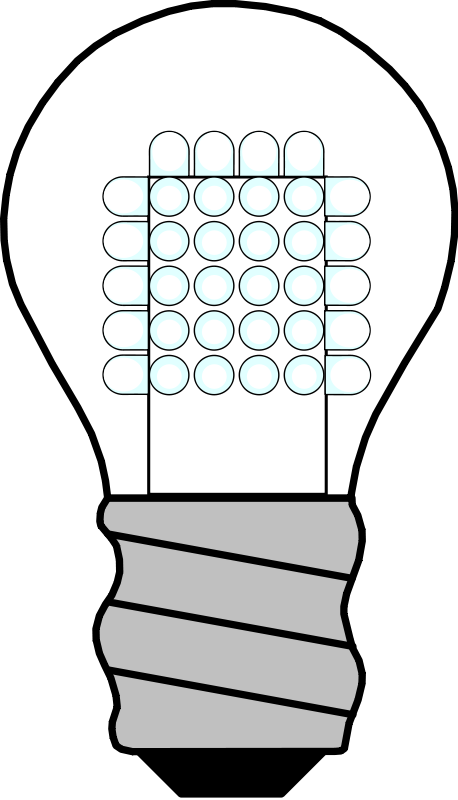
\includegraphics[scale=0.02]{imgs/bulb.png}
 \textbf{Nota} \\
 }%
{\endMakeFramed}

%Work in progress
\newenvironment{workinprogress}{%
  \def\FrameCommand{\colorbox{pink}}%
  \MakeFramed {\FrameRestore}
\lhdbend  \textbf{Work in progress} \\
 }%
{\endMakeFramed}

%Openquestion
\newenvironment{openquestion}{%
  \def\FrameCommand{\colorbox{pink}}%
  \MakeFramed {\FrameRestore}
 \textbf{Domanda aperta} \\
 }%
{\endMakeFramed}

%TODO
\newenvironment{todo}{%
  \def\FrameCommand{\colorbox{pink}}%
  \MakeFramed {\FrameRestore}
 \textbf{TODO} \\
 }%
{\endMakeFramed}

%%%%%%%%%%%%%%%%%%%%%%%%%%%%%%%%
%%%%%%%%%%%% HEADER %%%%%%%%%%%%
%%%%%%%%%%%%%%%%%%%%%%%%%%%%%%%%
\pagestyle{fancy}
% i comandi seguenti impediscono la scrittura in maiuscolo
% dei nomi dei capitoli e dei paragrafi nelle intestazioni
\renewcommand{\chaptermark}[1]{\markboth{#1}{}}
\renewcommand{\sectionmark}[1]{\markright{\thesection\ #1}}
\fancyhf{} % rimuove l'attuale contenuto dell'intestazione
% e del pi\`e di pagina
\fancyhead[LE,RO]{\bfseries\thepage}
\fancyhead[LO]{\bfseries\rightmark}
\fancyhead[RE]{\bfseries\leftmark}
\renewcommand{\headrulewidth}{0.5pt}
\renewcommand{\footrulewidth}{0pt}
\addtolength{\headheight}{0.5pt} % riserva spazio per la linea
\fancypagestyle{plain}{%
\fancyhead{} % ignora, nello stile plain, le intestazioni
\renewcommand{\headrulewidth}{0pt} % e la linea
}


%%%%%%%%%%%%%%%%%%%%%%%%%%%%%%%%
%%%%%%%%%%%% COLORS %%%%%%%%%%%%
%%%%%%%%%%%%%%%%%%%%%%%%%%%%%%%%
\definecolor{code}{gray}{0.3}


%%%%%%%%%%%%%%%%%%%%%%%%%%%%%%%%
%%%%%%%%%%%% NUMBERS %%%%%%%%%%%
%%%%%%%%%%%%%%%%%%%%%%%%%%%%%%%%
\setcounter{tocdepth}{3}
\setcounter{secnumdepth}{3}


%%%%%%%%%%%%%%%%%%%%%%%%%%%%%%%%
%%%%%%%%%%% DOC DATA %%%%%%%%%%%
%%%%%%%%%%%%%%%%%%%%%%%%%%%%%%%%
\title{Appunti di MNO}
\author{Gruppo Informatici Rampanti}
\date{ott 2010 - mag 2011}

\pdfinfo{%
  /Title    (Appunti di MNO)
  /Author   (Andrea Cimino e Lorenzo Muti)
  /Creator  (Andrea Cimino)
  /Producer (Lorenzo Muti)
  /Subject  (MNO)
  /Keywords (MNO)
}


%%%%%%%%%%%%%%%%%%%%%%%%%%%%%%%%
%%%%%%%%%%%%% UTILS %%%%%%%%%%%%
%%%%%%%%%%%%%%%%%%%%%%%%%%%%%%%%
% binary symbols
\newcommand{\modder}{\vdash _{R}}

% vertical gaps
\newcommand{\askip}{\vspace{0.5cm}}
\newcommand{\bskip}{\vspace{1.0cm}}

% various symbols
\newcommand{\qedhere}{\ensuremath{\Box}}
\newcommand{\qed}{\hfill \ensuremath{\Box}}

% substitution
\newcommand{\subst}[2]{^{#1} / _{#2}}

% denotational semantics function names
\newcommand{\bbracket}[1]{\left\llbracket #1 \right\rrbracket}

\newcommand{\aexpr}{\mathcal{A}}
\newcommand{\bexpr}{\mathcal{B}}
\newcommand{\cexpr}{\mathcal{C}}
\newcommand{\Aexpr}[1]{\mathcal{A} \bbracket{#1}}
\newcommand{\Bexpr}[1]{\mathcal{B} \bbracket{#1}}
\newcommand{\Cexpr}[1]{\mathcal{C} \bbracket{#1}}

\newcommand{\semdomset}[1]{(V_{#1})_{\bot}}

% semantic evaluations
\newcommand{\opereval}[3]{\left\langle #1, #2 \right\rangle \rightarrow #3}
\newcommand{\denaeval}[3]{\Aexpr{#1} #2 = #3}
\newcommand{\denbeval}[3]{\Bexpr{#1} #2 = #3}
\newcommand{\denceval}[3]{\Cexpr{#1} #2 = #3}

% rotated sqsubseteqs
\newcommand{\upsqsubseteq}{ $\begin{rotate}{90} $\sqsubseteq$ \end{rotate}$ }
\newcommand{\downsqsubseteq}{ $\begin{rotate}{270} $\sqsubseteq$ \end{rotate}$ }

% Space after paragraph declaration
\makeatletter
\renewcommand\paragraph{\@startsection{paragraph}{4}{\z@}%
  {-3.25ex\@plus -1ex \@minus -.2ex}%
  {1.5ex \@plus .2ex}%
  {\normalfont\normalsize\bfseries}}
\makeatother



% fast theorem and definition
\newcommand{\ftheo}[1]{\colorbox{YellowGreen}{#1}}
\newcommand{\fdefn}[1]{\colorbox{SkyBlue}{#1}}

\theoremstyle{break}
\theoremsymbol{\ensuremath{\clubsuit}}
\theoremseparator{\newline}
\newshadedtheorem{proc}[theo]{Procedura}

% bold math!
\newcommand{\bm}[1]{\mbox{\boldmath{$#1$}}}

\newcommand{\positive}[1]{\textbf{\color{green} +} #1}
\newcommand{\negative}[1]{\textbf{\color{red} -} #1}


\newtheoremlisttype{tab}%
{\begin{tabular*}{\linewidth}{@{}lrl@{\extracolsep{\fill}}r@{}}}%
{##1&##2&##3&##4\\}%
{\end{tabular*}}
\begin{document}
}
\providecommand{\outbpdocument}{\end{document}}
\else
\providecommand{\inbpdocument}{}
\providecommand{\outbpdocument}{}
\fi



\inbpdocument 

%% Bevilacqua 23 Novembre
\chapter{Risoluzione di Sistemi Lineari}

Siano $A \in \mathbb{C}^{n \times n}$ $x,b \in \mathbb{C}^{n}$ e si
supponga che il sistema lineare

$$Ax = b$$
sia consistente (ovvero, ammetta almeno una soluzione).\\ 
I metodi per risolvere il sistema si possono dividere in
\begin{itemize}
\item metodi diretti:
  \begin{itemize}
  \item Gauss
  \item Cholesky (Hermitiane definite positive)
  \item Householder (Maggiori garanzie di stablilit\`a)
  \end{itemize}
\item Metodi iterativi
\end{itemize}

\begin{notes}
  È possibile trattare tutti i metodi diretti come fattorizzazioni
  della matrice dei coefficienti della matrice lineare.
\end{notes}


\section{Propagazione dell'errore}
In un metodo diretto, se non ci fossero errori di rappresentazione dei
dati e di arrotondamento nei calcoli, la soluzione del sistema
verrebbe calcolata esattamente. Invece in un metodo iterativo, anche
nell’ipotesi che non ci siano errori di rappresentazione dei dati e di
arrotondamento nei calcoli, si deve comunque operare un troncamento
del procedimento, commettendo un errore, detto \emph{errore analitico}.\\

Una maggiorazione dell’errore da cui \`e affetta la soluzione può essere
rappresentata da due termini distinti:
\begin{itemize}
\item l'\emph{errore inerente}, dovuto agli errori di rappresentazione dei dati,
che non dipendono dal particolare metodo usato, e
\item l'\emph{errore algoritmico}, dovuto agli errori di arrotondamento nei calcoli,
che dipende dal metodo usato, ma non dagli errori sui dati.
\end{itemize}

Lo studio dell’errore inerente può essere fatto perturbando i dati ed
esaminando gli effetti indotti sulla soluzione.

\begin{theo}[Numero di condizionamento di $A$]
Siano $\delta A \in \mathbb{C}^{n \times n}$ e $\delta b \in
\mathbb{C}^n$ rispettivamente la matrice e il vettore delle
perturbazioni sui dati del sistema, dove $b \neq 0$ e sia $|| \cdot
||$ una qualunque norma indotta. Se $A$ non \`e singolare e se $||
A^{-1}|| \; || \delta A|| < 1$ allora anche la matrice $A + \delta A$
\`e non singolare. Indicata con $x + \delta x$ la soluzione del sistema perturbato
$$(A + \delta A) (x + \delta x) = b + \delta b$$

risulta 
$$ \frac{||\delta x||}{||x||} \leq \mu(A)
\frac{ \frac{|| \delta A||}{||A||} + 
\frac{|| \delta b||}{||b||}}{1 - \underbrace{\mu(A) \frac{||\delta A||}{||A||}}_{<1}}
$$
in cui $ \mu(A)  = ||A|| \; ||A^{-1}|| $ \`e detto \emph{numero di
  condizionamento} della matrice $A$
\end{theo}

Si osservi che il numero di condizionamento \`e sempre maggiore o
uguale a 1. Inoltre se $\mu(A)$ assume valori piccoli, allora piccole
perturbazioni sui dati inducono piccole perturbazioni sulla soluzione
e la matrice del sistema \`e ben condizionata.\\
Un metodo risulta più \emph{stabile} di un altro se \`e meno sensibile
agli errori indotti dai calcoli. Lo studio della stabilit\`a di un
metodo perde di significativit\`a quando il problema \`e fortemente mal
condizionato, poich\'e in questo caso l’errore inerente prevale
sull’errore algoritmico.




\section{Fattorizzazione}
I metodi diretti che vedremo utilizzano una fattorizzazione della
matrice A, nel prodotto di due matrici B e C, facilmente invertibili.
$$ A = BC $$
Possiamo dunque riscrivere il sistema, e la sua soluzione si riduce
alla risoluzione di due sottoproblemi:
$$ BCx = b \qquad
\left\{ 
  \begin{array}{l}
  By = b\\
  Cx = y                                         
  \end{array}
\right.
$$
$B$,$C$ possono appartenere alle seguenti classi:
\begin{itemize}
 \item Triangolari (Si risolve per sostituzione
   all'indietro). $O(n^2)$ operazioni.
 \item Unitarie (Sono facili da invertire). Infatti
     $Qx =b \rightarrow x =Q^{H}b$. $O(n^2)$ operazioni.
\end{itemize}

Vedremo le seguenti 3 fattorizzazioni classiche. \\

$A = LU$
\begin{itemize}
\item $L$ \`e triangolare inferiore (Lower) con diagonale unitaria ($l_{ii}=1$)
\item $U$ \`e triangolare superiore (Upper)
\item associata al metodo di Gauss.
\end{itemize}

$A = LL^{H}$
\begin{itemize}
\item $L$ \`e triangolare inferiore con elementi positivi sulla
  diagonale ($\mathbb{R} \ni l_{ii}>0$)
\item associata al metodo di Cholesky.
\end{itemize}

$A = QR$
\begin{itemize}
\item $Q$ unitaria 
\item $R$ triangolare superiore
\item associata al metodo di Householder.
\end{itemize}

Se la matrice $A$ \`e reale, le matrici delle tre fattorizzazioni, quando
esistono, sono reali.\\
Il costo computazionale della fattorizzazione \`e $O(n^3)$ operazioni,
mentre il costo computazionale della risoluzione dei sistemi \`e
$O(n^2)$ operazioni.\\
La fattorizzazione $QR$ esiste per ogni matrice $A$, mentre non sempre \`e
possibile ottenere le fattorizzazioni $LU$ e $LL^H$. Valgono infatti i
seguenti teoremi.

\paragraph{Fattorizzazione LU}
\begin{theo}[Esistenza della fattorizzazione $A=LU$]\label{th:LU}
Sia $A$ una matrice di ordine $n$ e siano $A_k$ le sue sottomatici
principali di testa di ordine $k$. Se $A_k$ \`e non singolare per
$k=1,\ldots,n-1$ allora esiste ed \`e \emph{unica} la fattorizzazione
$LU$ di $A$.
\end{theo}

\begin{thproof}
  Per induzione su $n$
  \begin{itemize}
  \item $n=1$\\
    \[\begin{array}{ccc}
      a_{11} = & 1 \cdot & a_{11} \\ 
      A        & L       & U
    \end{array}\]
    (oppure $a_{11}$ potrebbe essere uguale a $0$).
 \item $n>1$\\
\[
A = \left |
\begin{array}{c|c}
A_{n-1} & \mathbf{d} \\ \hline
\mathbf{c}^{H} &  \alpha
\end{array}
\right | = \left |
\begin{array}{c|c}
L_{n-1} & \mathbf{0} \\ \hline
\mathbf{u}^{H} &  1
\end{array}
\right |
\cdot
\left |
\begin{array}{c|c}
U_{n-1} & \mathbf{v} \\ \hline
\mathbf{0}      & \beta
\end{array}
\right |
\]
Otteniamo le sequenti equazioni:
\[\left\{
  \begin{array}{ll}
    A_{n-1} = L_{n-1} \cdot U_{n-1} & (1) \\
    d = L_{n-1} \cdot v           & (2)  \\
    c^{H} = u^{H} \cdot U_{n-1} \quad \rightarrow \quad 
    c = U^{H}_{n-1} \cdot u \quad  & (3) \\
    \alpha = u^{H} \cdot v + \beta &(4) \\
  \end{array}
\right.\]
Da cui traiamo le seguenti:
\begin{itemize}
\item $(1)$ essendo $L_{n-1}$ triangolare inferiore $det(L_{n−1}) =
  \Pi_{i=0}^{n-i} l_{ii} = 1$ allora $det (U_{n-1}) = det(A_{n-1})$ che
  per ipotesi \`e diverso da zero. Quindi esistono le inverse di $L$ e $U$
  e i seguenti valori sono determinati univocamente.
\item $(2)$ $v = L^{-1}_{n-1} \cdot d$ 
\item $(3)$ $u = (U_{n-1}^{H})^{-1} \cdot c$
\item $(4)$ $\beta = \alpha - u^{H} \cdot v$ 
\end{itemize}
\end{itemize}
\end{thproof}

Se cade l'ipotesi del teorema perdiamo l'unicit\`a, possiamo non avere
alcuna fattorizzazione o averne più di una.
\begin{example}[Fattorizzazione non unica]
\[ 
A = 
\begin{pmatrix}
0 & 1 \\
0 & 2 
\end{pmatrix}
= \underbracket{
\begin{pmatrix}
1 & 0  \\
l & 1 
\end{pmatrix}}_{L}
\cdot \underbracket{
\begin{pmatrix}
0 & 1  \\
0 & u 
\end{pmatrix}}_{U}
\]
esistono infinite combinazioni per cui vale $l+u=2$.
\end{example}

\begin{theo}
  Per ogni matrice A, esiste una matrice di permutazione $\Pi$ per cui
  si può ottenere la fattorizzazione $LU$ di $\Pi A$, cio\`e
  $$\Pi A = LU$$
\end{theo}

%  TODO COSA È QUESTA??
% $$
% \[
% \left(
% \begin{array}{c|ccc}
%   a_{11} & 1 & 1 & 1 \\ \hline \\[-9pt]
%   0 & \multicolumn{3}{c}{\multirow{4}{*}{\Huge $C$}} \\[-4pt]
%   \vdots & \\
%   0 &
% \end{array}
% \right)
% \]
% $$

\paragraph{Fattorizzazione $LL^{H}$}
\begin{theo}[Esistenza fattorizzazione $LL^{H}$]\label{th:esistenza-LL}
Sia A una matrice hermitiana definita positiva, allora esiste ed \`e
unica la fattorizzazione $LL^H$ di A.
\end{theo}

\begin{thproof}
  con $l_{ii} > 0$. \\
  Per il teorema \ref{richiamibevilacqua:definitepositive},
  $A$ ha le sottomatrici $A_k$ con $det(A_k) > 0$ e quindi per il
  teorema \ref{th:LU} esiste unica la fattorizzazione (per evitare
  confusione rinominiamo L con M):
  $$ A = M \cdot U $$
  in cui ricordiamo che M \`e triangolare inferiore $m_{ii}=1$ e U \`e
  triangolare superiore. Possiamo scomporre ancora:
  $$ A = M \cdot \underbracket{D \cdot R}_{U}$$
  Con D matrice diagonale i cui elementi principali sono quelli di U,
  e R triangolare superiore con $r_{ii} = 1$.

  $$
  \underbracket{
    \begin{pmatrix}
      u_{11} & u_{12}  \\
      0     & u_{22}
    \end{pmatrix}}_{U} = \underbracket{
    \begin{pmatrix}
      u_{11} & 0  \\
      0     & u_{22}
    \end{pmatrix}}_{D} \underbracket{
    \begin{pmatrix}
      1 & \frac{u_{12}}{u_{11}} * \\
      0 & 1
    \end{pmatrix}}_{R}
  $$
* \`e possibile solo se $det(A)\neq0$ ed \`e effetivamente così nel nostro
caso, infatti $\left\{
  \begin{array}{l}
    det(U) \neq 0 \\
    det(A) > 0
  \end{array}
\right.$

Dalla propriet\`a delle hermitiane $A^{H} = A$ otteniamo:
$$ \underbracket{R^{H}}_{L}\underbracket{D^{H} M^{H}}_{U} =
\underbracket{M}_{L}\underbracket{DR}_{U} $$ dato che abbiamo da entrambi i lati
la fattorizzazione LU, dalla sua unicit\`a otteniamo: 
\[\begin{array}{l}
  R^{H} = M \; \Rightarrow \; M^{H} = R \\
  DR = D^{H}M^{H}= D^{H}R  \Rightarrow  D = D^{H}
\end{array}\]
Sappiamo quindi che $d_{ii}  = \overline{d}_{ii}$, quindi $D \in
\mathbb{R}$.\\

Vogliamo ora dimostrare che D \`e hermitiana definita positiva, partiamo
dalla definizione:
$$ x^{H}Dx = \underbracket{x^{H} M^{-1}}_{y^{H}}
\underbracket{MDM^{H}}_{A} \underbracket{(M^{H})^{-1} x}_{y} = y^{H}Ay
\underbracket{>}_{A\;def\;pos} 0 $$
Quindi possiamo concludere che anche $D$ \`e diagonale ed hermitiana
definita positiva, ed avendo solo autovalori positivi, avr\`a $d_{ii}>0$.\\

Esiste allora un’unica matrice diagonale $F$ ad elementi principali
reali e positivi, tale che $D = F^2$, e quindi $F =
diag\{\sqrt{d_{ii}}\}$. Da cui possiamo ricavare:

$$ A = MDR = \underbracket{M F} \underbracket{F^H M^H} = LL^H $$

Notare che la fattorizzazione di Cholesky \`e \emph{caratterizzante}: se
A \`e fattorizzabile $LL^H$ allora \`e hermitiana definita positiva.
\end{thproof}


\paragraph{Fattorizzazione QR}\label{fatt:QR}
A differenza della fattorizzazione $LU$ e $LL^H$ , la fattorizzazione $QR$ di
una matrice A non \`e unica. 

\begin{observation}
  Se Q e R esistono, non sono uniche.
\end{observation}
\begin{thproof}
  Se $A = QR = Q \underbracket{D D^{-1}}_{I} R$  \\
  e scegliamo $D$ come matrice diagonale e unitaria, quindi con $|d_{ii}| = 1$, abbiamo
  $$ D D^H = 
  \begin{array}{|ccc|}
    \ddots & & \\
    & d_{ii} \cdot \overline{d}_{ii} & \\
    & & \ddots
  \end{array}
  = I $$
e possiamo scrivere 
$$ A = QR = \underbracket{Q D}_{\text{unit}}
\underbracket{D^{H} R}_{\text{tri. sup}} = Q_1 R_1 $$
quindi abbiamo ottenuto un'altra fattorizzazione.\\
Le matrici D vengono dette \emph{matrici di fase} ed solo con queste
che la fattorizzazione non \`e unica, quindi possiamo dire che la
fattorizzazione QR \`e unica a meno di matrici di fase.
\end{thproof}


La determinazione delle matrici della fattorizzazione di A viene 
generalmente effettuata nei due modi seguenti:
\begin{itemize}
\item applicando alla matrice A una \emph{successione di matrici
    elementari}  (metodo di Gauss, metodo di Householder);
\item con \emph{tecniche compatte} (metodo di Cholesky).
\end{itemize}

\section{Metodo di Gauss}
Nel metodo si ricava una incognita da una delle equazioni e si
sostituisce in tutte le altre, ripetendo il procedimento fino a
trovare la soluzione (nella variante classica impone una certa
strategia nella risoluzione).\\
Il cambiamento della matrice dovuto alla sostituzione dei coefficienti
può essere espresso come la moltiplicazione per una matrice E:
$$ E A^{(1)} = A^{(2)} $$

Dove  $A^{(1)}$ e $A^{(2)}$ sono la matrici prima e dopo la sostituzione.
La matrice $E$ \`e detta \emph{elementare} ed ha diagonale unitaria e la
prima colonna diversa da zero.

\[
E = \left |
\begin{array}{ccccc}
1      &   &  & \multicolumn{2}{c}{\multirow{2}{*}{\huge $0$}}      \\
x_2    & 1 &  &                                                     \\
\vdots & \multicolumn{2}{c}{\multirow{2}{*}{\huge $0$}} & \ddots &  \\
x_n    &   &  & &1
\end{array}
\right |
\]

Facendo i passi sequenti avremo:
$$ E^{(S)} \ldots E^{(2)} \cdot E^{(1)} \cdot A^{(1)} = U $$
con $U$ triangolare superiore.
Ora portando al secondo membro:
$$ A = A^{(1)} = \underbracket{(E^{(S)} \ldots E^{(1)})^{-1}}_{L} U $$


$$ A^{(n)} = E^{(n-1)}\ldots E^{(2)} E^{(1)}A$$
\begin{defn}[Matrice Elementare]
Siano $\sigma \in \mathbb{R}$ e $u,v \in \mathbb{C}^n, u,v, \neq
0$. Si definisce \emph{matrice elementare}:
$$ E(\sigma, \mathbf{u},\mathbf{v}) = 
   I - \sigma \mathbf{uv}^{H} $$


\[\left | \begin{array}{ccccc}
    1  &   &  & \multicolumn{2}{c}{\multirow{2}{*}{\huge $0$}}      \\
       & 1 &  &                                                     \\
    \multicolumn{2}{c}{\multirow{2}{*}{\huge $0$}}  &   & \ddots &  \\
       &  & & & 1
\end{array} \right |
-\sigma
\left | \begin{array}{c}
    x \\
    x \\
    \vdots \\
    x
\end{array} \right |
|x \; x \; \cdots \; x|
\]
\end{defn}

\begin{notes}\textbf{Perch\'e calcola questi autovalori come se la diade fosse singolare?}\\
  $\sigma u v^{H}$ \`e detta \emph{diade} ed ha rango $\leq 1$,
  TODO???$det(\sigma u v^{H}) = 0$.\\
I suoi autovalori sono:
\begin{itemize}
\item $\lambda_1 = 0$  (molteplicita $n-1$)
\item $\lambda_2 = \sigma v^{H} u$   (molteplicit\`a $1$)
\end{itemize}

Quindi gli autovalori di $E$ sono:
$\left\{ 
 \begin{array}{ll}
 1-0 = 1            & \text{molt. n-1} \\
 1 - \sigma v^{H} u & \text{molt. 1}
\end{array}
\right.$\\
dai quali ricaviamo il determinante di E: $det(E) = 1 (1 - \sigma v^H
u) \neq 0$.\\
Quindi $E$ \`e invertibile se e solo se $\sigma v^{H}u \neq 1$, infatti
questa condizione \`e l'ipotesi del seguente teorema che ci permette di
calcolare l'inversa di una matrice elementare.
\end{notes}

La classe delle matrici elementari non singolari \`e chiusa rispetto
all'operazione di inversione. Vale infatti il seguente teorema.

\begin{theo}[Invertibilit\`a matrici elementari]
\label{th:eleminversa}
  Ogni matrice elementare $E(\sigma, \mathbf{u, v})$ per cui $\sigma
  \mathbf{v}^H \mathbf{u} \neq 1$ \`e invertibile e la sua inversa \`e
  ancora una matrice elementare della forma e $E(\tau, \mathbf{u, v}),
  \tau \in \mathbb{C}$.
\end{theo}

\begin{thproof}
Se $\sigma=0$ la tesi \`e ovvia. Per $\sigma \neq 0$ dimostriamo che
esiste un $\tau$ tale che:
\[\begin{array}{ll}
 (I - \sigma uv^{H})(I - \tau u v^{H}) = I \\
 \cancel{I} - (\sigma + \tau) uv^{H} + \sigma \tau u 
 \underbracket{v^{H} u}_{scalare} v^{H} = \cancel{I} \\
 \underbracket{(-\sigma - \tau +  \sigma \tau v^{H}
   u)}_{\text{scalare}} \underbracket{uv^{H}}_{\text{matrice}} = 0 
\end{array}\]

Per non cadere nel caso in cui $E=I$, poniamo che n\'e $u$ n\'e $v$ siano
nulli. Allora possiamo concludere che
\[\begin{array}{ll}
 - \sigma - \tau + \sigma\tau v^{H} u = 0 \\
 \tau(-1 + \sigma v^{H}u) = \sigma \\
 \tau = \frac{\sigma}{\sigma v^{H}u-1} 
\end{array}\]
che esiste perch\'e per ipotesi $\sigma v^{H}u \neq 1$.
\end{thproof}

Vogliamo usare le matrici elementari per il metodo Gauss, e quindi ci
chiediamo se esista una $E$ tale che $A^{(2)} = E A^{(1)}$, questo ci \`e
garantito dal teorema seguente.

\begin{theo}\label{th:elem}
  Siano $x,y \in \mathbb{C}^n$, $x,y \neq \mathbf{0}$. Esistono matrici
  elementari non singolari $E(\sigma, u, v)$ tali che 
  $$ E(\sigma, u, v)x = y $$
\end{theo}

\begin{thproof}
 Vogliamo mostrare che:
  $$ (I - \sigma uv^{H}) x = y$$
  $$ x - \sigma u v^{H} x = y $$
  $$ \sigma u = \frac{x -y} {v^{H}x}$$
  Quindi la prima condizione \`e che $v^{H}x \neq 0$.\\ 
  Inoltre per avere $E$ invertibile \`e necessario che $\sigma
  v^{H}u \neq 1$, da cui

  $$ v^{H}\underbracket{\sigma u} = v^{H} \frac{x - y}{v^{H}x} = 
  \frac{v^{H}x}{v^{H}x} - \frac{v^{H}y}{v^{H}x}
  = 1 - \frac{v^{H}y}{v^{H}x} \neq 1 $$ 
  $$ \frac{v^{H}y}{v^{H}x} \neq 0 \quad \Rightarrow \quad v^{H}y \neq 0 $$
  Quindi per ottenere la matrice E basta rispettare il seguente sistema:
  $$ v:  \left\{
    \begin{array}{ll}
      v^{H} x \neq 0 & \text{esistenza}\\
      v^{H} y \neq 0 & \text{invertibilit\`a}
    \end{array}
  \right.
  $$
\end{thproof}

\section{Matrici Elementari di Gauss}
Vediamo ora quali matrici elementari sono adatte per il metodo di Gauss.\\
Sia $\mathbf{x}$, con $x_1 \neq 0$. Si vuole determinare una matrice

$$ M = E(\sigma, \mathbf{u},\mathbf{e}_1 ) = I - \sigma \mathbf{u} {\mathbf{\underbracket{\mathbf{e}_1}_{v}}}^H
\qquad 
\mathbf{e}_1 = | \; 1 \; 0 \; \cdots \; 0 \; |^{T} 
$$
tale che
$$ M\mathbf{x} = \underbracket{x_1 \mathbf{e}_1}_{\mathbf{y}} = 
| \; x_1 \; 0 \; \cdots \; 0 \; |^T
$$
cio\`e "proietti" la prima componente del vettore $\mathbf{x}$.
Dobbiamo quindi trovare  $\sigma$ ed  $\mathbf{u}$ per cui valga questa
condizione.
\paragraph{Esistenza}
 Per stabilire l'esistenza di $M$: sappiamo che vale la condizione
% \[\left\{
% \begin{array}{ll}
% \mathbf{e}_1^{H} \mathbf{x} = x_1 \neq 0                             \\
% \mathbf{e}_1^{H} x_1 \mathbf{e}_1 = x_1 \neq 0                        \\
% \end{array}
% \right.
% \quad \Longrightarrow \quad
% x_1 \neq 0
% \]
  $$\mathbf{e}_1^{H} \mathbf{x} = x_1 \neq 0$$
 Ed il teorema \ref{th:elem} ci dice che questa condizione \`e sufficiente
 per l'esistenza.\\
Quindi
$$ \sigma \mathbf{u} = \frac{\mathbf{x}-\mathbf{y}}{\mathbf{v}^{H}\mathbf{x}}
=  \frac{\mathbf{x} - x_1\mathbf{e}_1}{\mathbf{e}^{H}_1\mathbf{x}}
=  \frac{\mathbf{x} - x_1\mathbf{e}_1}{x_1} = \frac{1}{x_1}
\begin{array}{|l|}
  0                                               \\
  x_2                                             \\ 
  \vdots                                          \\ 
  x_n
\end{array} 
=
\begin{array}{|l|}
  0                                               \\
  \frac{x_2}{x_1}                                 \\ 
  \vdots                                          \\ 
  \frac{x_n}{x_1}
\end{array} $$

 
La matrice $M^{(1)}$ \`e perció:
\[M^{(1)} = 
\begin{pmatrix}
1                &   &        &                   \\
-\frac{x_2}{x_1} & 1 &        &                   \\
\vdots           &   & \ddots &                   \\
-\frac{x_n}{x_1} &   &        & 1 
\end{pmatrix}\]

\paragraph{Matrice inversa}
 La matrice $M$ risulta invertibile sfruttando \ref{th:eleminversa}, in quanto
$$ \sigma \mathbf{e}_1^{H}\mathbf{u} = 0$$

Possiamo quindi calcolare la  sua inversa, partendo dal valore di $\tau$:
$$ \tau = \frac{\sigma}{\sigma \underbracket{\mathbf{v}^{H}\mathbf{u}}_{=0}-1}= -\sigma$$
Nel caso del metodo di Gauss $v^{H}u = 0$ dato che $v^{H}=|1 \; 0 \; \ldots
\; 0|$ e $u = |0 \; x \; \ldots \; x|^{-1}$.\\
Quindi in generale una matrice inversa della elementare di Gauss \`e data da
$$ M^{-1} = I + \sigma \mathbf{u} \mathbf{e}_1^{H} $$

nel nostro caso:
\[(M^{(1)})^{-1} = 
\begin{pmatrix}
1               &   &        &                   \\
\frac{x_2}{x_1} & 1 &        &                   \\
\vdots          &   & \ddots &                   \\
\frac{x_n}{x_1} &   &        & 1 
\end{pmatrix}\]

Le matrici elementari hanno la propriet\`a di trasformare un
qualunque vettore non nullo in un vettore con al più una componente
diversa da zero. Quindi possiamo sfruttarle per trasformare in forma
triangolare superiore una matrice, moltiplicandola successivamente per
opportune matrici elementari.\\
Al $k$-esimo passo, posto $a^{(k)}_{kk} \neq 0$ si considera il vettore 
$$ m^{(k)} = | \; \underbracket{0 \; \cdots \; 0}_{k\text{ componenti}} m_{k+1,k} \; \cdots \; m_{nk} \; |^T $$
dove $m_{ik} = a^{(k)}_{ik} / a^{(k)}_{kk}$ con $i = k+1,\ldots,n$ da
cui ricaviamo 

\[ E^{k} = E(1,m^{(k)}, e_k) = M^{(k)} =
\begin{pmatrix}
1 &        &            &        & \\
  & \ddots &            &        & \\
  &        & 1          &        & \\
  &        & -m_{k+1,k} &        & \\
  &        & \vdots     & \ddots & \\
  &        & -m_{nk}    &        & 1 
\end{pmatrix}\]

Poniamo ora 
$$ U = A^{(n)} = M^{(n-1)} \ldots M^{(2)} M^{(1)} A $$

Possiamo utilizzare l'inversione delle $M$, ottenendo quindi
$$ \underbracket{(M^{(1)})^{-1} \ldots (M^{(n-2)})^{-1} (M^{(n-1)})^{-1}}_{L} U = A $$
\[ L = (M^{(1)})^{-1} \ldots (M^{(n-1)})^{-1} = 
\begin{pmatrix}
1      &        &           &        &           & \\
m_{21} & \ddots &           &        &           & \\
       & \ddots & 1         &        &           & \\
\vdots &        & m_{k+1,k} &        &           & \\
       &        & \vdots    & \ddots & \ddots    & \\
m_{n1} & \cdots & m_{nk}    & \cdots & m_{n,n-1} & 1
\end{pmatrix}\]



\begin{figure}[h]
 \centering
 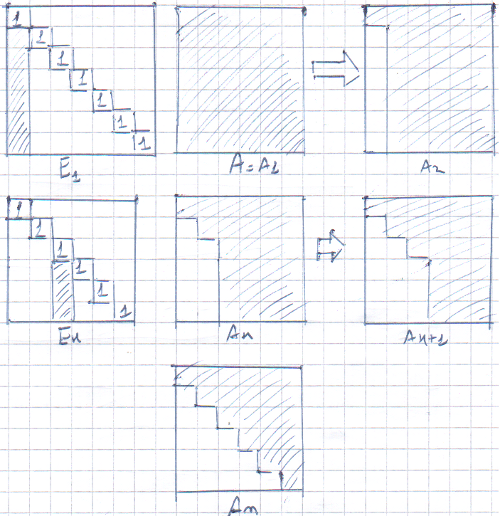
\includegraphics[width=0.40\textwidth]{./imgs/lu.png}
 % lu.png: 500x516 pixel, 150dpi, 8.47x8.74 cm, bb=0 0 240 248
 \caption{Passi della trasformazione $LU$ per mezzo di matrici elementari di Gauss}
\end{figure}

% Vediamo il secondo passo di questo processo:
% \[\begin{array}{cccc}
% M^{(2)} &A^{(2)} &= &A^{(3)} \\
% % TODO verificare come \`e fatta questa matrice
% \begin{pmatrix}
% 1      & 0      & 0 & \ldots & 0                  \\
% 0                                                 \\
% 0                                                 \\
% \vdots                                            \\
% 0                
% \end{pmatrix}
% &
% \begin{pmatrix}
% x      & x      & x & \ldots & x                  \\
% 0      & x      & x & \ldots & x                  \\
% 0      & x      & x & \ldots & x                  \\
% \vdots & x      & x & \ldots & x                  \\
% 0      & x      & x & \ldots & x
% \end{pmatrix}
% &
% &\begin{pmatrix}
% x      & x      & x & \ldots & x                  \\
% 0      & x      & x & \ldots & x                  \\
% 0      & 0      & x & \ldots & x                  \\
% \vdots & \vdots & x & \ldots & x                  \\
% 0      & 0      & x & \ldots & x
% \end{pmatrix}
% \end{array}\]


Quindi il procedimento consiste nel prodotto di n matrici triangolari
inferiori con elementi diagonali uguali a 1, ed il risultato \`e ancora
una matrice di questa forma, quindi compatibile con la nostra
definizione di matrice $L$ del metodo $LU$.

\begin{example}
Per n = 4
$$ (M^{(1)})^{-1} (M^{(2)})^{-1}(M^{(3)})^{-1} = 
\begin{pmatrix}
  1      &        &        & \\
  m_{21} & 1      &        & \\
  m_{31} &        & 1      & \\
  m_{41} &        &        & 1
\end{pmatrix}
\begin{pmatrix}
  1      &        &        & \\
         & 1      &        & \\
         & m_{32} & 1      & \\
         & m_{42} &        & 1
\end{pmatrix}
\begin{pmatrix}
  1      &        &        & \\
         & 1      &        & \\
         &        & 1      & \\
         &        & m_{43} & 1
\end{pmatrix} =
\begin{pmatrix}
  1      &        &        & \\
  m_{21} & 1      &        & \\
  m_{31} & m_{32} & 1      & \\
  m_{41} & m_{42} & m_{43} & 1
\end{pmatrix} = L
$$
\end{example}

L'elemento $a_{kk}$ della matrice $A^{(k)}$, detto \emph{pivot} al
k-esimo passo, \`e per ipotesi diverso da zero e dato che $A^{(k)}$ \`e
triangolare superiore per \ref{triangolari}
$$ \det(A_k) = a^{(1)}_{11} \cdot \ldots \cdot a^{(k)}_{kk} \neq 0 $$
quindi $A^{(k)}$, detta minore principale di testa, \`e non singolare.

% TODO Cosa avr\`a voluto dire?
% $$ A^{(k)} = M^{(k-1)} \ldots M^{(1)} A^{(1)} $$
% La sottomatrice superiore sinistra () $B$
% $k \times k$, viene raggiunta quanto si arriva ad usare $M^{(k-1)}$, 
% allora sappiamo che il determinante di $B$ \`e il prodotto degli
% $a^i_{ii}$ per \ref{triangolari}
% Il Minore principale di testa \`e uguale al prodotto dei minori principali di testa di 
% $$ M^{(k-1)} \ldots M^{(1)}A^{(1)} $$
% Quindi abbiamo $a_{kk}^{(k)} = det A_k \neq 0 $ (gli M sono nulli)

%% 7 Dicembre
\section{Matrici elementari di Householder}
\label{sec:householder}
% TODO
% $P^{(i)}$ matrici elementari \emph{unitarie} perche vogliamo $Q$ unitaria.
% Inoltre $P^{(i)}$ unitaria Hemitiane \\
% Avremo 
% $Px = [ \alpha, 0 ,0,\ldots, 0] = \alpha e_1$
Il procedimento di fattorizzazione della matrice A con matrici di
Householder \`e sempre applicabile. Queste matrici ci servono per
costruire la fattorizzazione $QR$.
$$ A = \underbracket{Q}_{\text{unitaria}}\cdot\underbracket{R}_{\text{tr. sup.}} $$

Dobbiamo trovare una matrice elementare  $P$ unitaria tale che
$$ P_{n-1} \ldots P_{1} \cdot A = R$$
$$ A = \underbracket{(P_{n-1}\ldots P_{1})^{-1}}_{Q}R $$

\begin{defn}[Matrice elementare di Householder]
  Una matrice elementare hermitiana
  $$ P = I - \beta \mathbf{\mathbf{v} \mathbf{v}}^H $$
  con $\beta \in \mathbb{R}$ e $\mathbf{v} \in \mathbb{C}^n,\mathbf{v} \neq 0$, \`e detta
  \emph{matrice di Householder} se \`e unitaria, cio\`e se $P^H P = P P^H = I$.
\end{defn}

Per ogni vettore $\mathbf{x} \in \mathbb{C}^n$, con $\mathbf{x} \neq 0$, si può
determinare una matrice di Householder $P$ tale che 
 $$ P\mathbf{x} = \alpha \mathbf{e}_1 $$ 
dove $\alpha$ \`e una opportuna costante e $\mathbf{e}_1$ \`e il primo vettore della base canonica. Nel metodo, $x$ assumerà i valori delle colonne di $A$, dalla prima all'$n$-esima, che si vorranno trasformare.

\begin{property}
  La matrici unitarie godono della seguenti propriet\`a:
  \begin{itemize}
  \item $$ U^{-1} = U^{H}$$
  \item moltiplicare per una matrice unitaria non cambia la norma 2
    $$ || U\mathbf{x} ||_{2} = || \mathbf{x} ||_{2} \quad \text{vettori}$$
    $$ || UM ||_{2} = || M ||_{2} \quad \text{matrici}$$
    Per quanto riguarda le norme di vettori infatti,
    ricordando che 
    $$||\mathbf{x}|| \defeq \sqrt{\mathbf{x}^{H}\mathbf{x}} =
    \sqrt{\displaystyle \sum_{i}^{n} |x_i|^{2}}$$
    otteniamo
    $$ || U\mathbf{x} ||_{2} = \sqrt{(U\mathbf{x})^{H} U\mathbf{x}} =
    \sqrt{\mathbf{x}^{H}U^{H}U\mathbf{x}} = \sqrt{\mathbf{x}^{H}\mathbf{x}} =
    ||\mathbf{x}||_{2}$$
    Invece per le matrici consideriamo la norma indotta (spettrale) $\rho$.
    Ricordando che
    $$||M||_2 \defeq \sqrt{\rho(M^{H}M)}$$
    otteniamo

    $$ || UM ||_{2} = \sqrt{\rho\left((UM)^{H} UM \right)} = \sqrt{\rho(M^{H}U^{H}UM)} = \sqrt{\rho(M^{H}M)} = ||M||_{2} $$
    Quindi la matrice unitaria \`e una trasformazione che conserva le lunghezze:
    una \emph{isometria}
\end{itemize}
\end{property}

Quindi, nel procedimento che useremo, conserveremo le lunghezze, e questo
\`e importante per la stabilit\`a.\\

\paragraph{Condizioni per $\beta$}
Dal fatto che P \`e unitaria e hermitiana ricaviamo:
$$ I \underbracket{=}_{unit.} PP^{H} \underbracket{=}_{herm.} PP = 
(I - \beta \mathbf{v}\mathbf{v}^{H})(I - \beta \mathbf{v}\mathbf{v}^{H}) = 
\cancel{I} - 2\beta \mathbf{v}\mathbf{v}^{H} + \beta^{2} \mathbf{v} \underbracket{\mathbf{v}^{H}\mathbf{v}}_{scalare}\mathbf{v}^{H} = 
\cancel{I} $$
%\[\begin{array}{ll}
In sostanza dobbiamo rispettare la condizione 
$$ \beta(-2\mathbf{v}\mathbf{v}^{H} + \beta \mathbf{v}^{H}\mathbf{v} \mathbf{v}\mathbf{v}^{H}) = 0 $$
Ponendo la condizione $\beta \neq 0$
   $$( -2 + \beta \mathbf{v}^{H}\mathbf{v}) \mathbf{v}\mathbf{v}^{H} = 0$$ 
e  ponendo $\mathbf{v} \neq 0$, come richiesto dalla
   definizione di elementare di Householder, otteniamo
  $$ \beta = \frac{2}{\mathbf{v}^{H}\mathbf{v}} = 
  \frac{2}{||\mathbf{v}||^{2}_{2}}
    $$
% &
  % \mathbf{0} \text{ (caso banale), come da definizione} \\ \\
  % \beta = \frac{2}{\mathbf{v}^{H}\mathbf{v}} = \frac{2}{||\mathbf{v}||^{2}_{2}} &
  % \text{condizione per unitariet\`a}
%\end{array}\]

\paragraph{Condizioni per $\alpha$}
Inoltre dato che $P\mathbf{x} = \alpha \mathbf{e}_1$ e P \`e unitaria abbiamo la seguente condizione su $|\alpha|$
$$ ||\mathbf{x}||_2 = ||P\mathbf{x}||_2 = || \alpha e_{1}||_2 = |\alpha| $$

Inoltre dalle propriet\`a delle hermitiane risulta $ \mathbf{x}^{H}P\mathbf{x} \in
\mathbb{R}$, da cui:
$$ \mathbb{R} \ni \mathbf{x}^{H}P\mathbf{x} = \mathbf{x}^{H} \alpha \mathbf{e}_1 = \overline{x}_1 \alpha = \ldots $$
                                                               \\
Ora esprimiamo
\[\begin{array}{rll}
 \alpha         & = |\alpha| &(\cos(\varphi) + i \sin (\varphi)) \\
 x_1            & = |x_1| &(\cos(\psi)      + i \sin (\psi))  \\
 \overline{x_1} & = |x_1| &(\cos(-\psi)    + i \sin (-\psi))
\end{array}\]
Ricordando dalla trigonometria che
$$
\begin{array}{l}
\mathbb \mathrm{sen} \, (\alpha - \beta)=\mathrm{sen} \, \alpha \, \cos\beta - \cos\alpha \, \mathrm{sen} \, \beta \\
\mathbb \cos(\alpha - \beta)=\cos\alpha \, \cos\beta + \mathrm{sen} \, \alpha \, \mathrm{sen} \, \beta   
\end{array}
$$
otteniamo
$$ \ldots = |x_1| |\alpha| (\cos(\varphi - \psi) + i \sin(\varphi - \psi))$$
% x_1 x_2 .... x_n  \alpha
%                     0
%                     0
%                     0
%                     0
%                     0
Affinch\'e questo numero sia reale \`e necessario annullare la sua parte
immaginaria. \\
$$ \sin(\varphi - \psi) = 0 
\quad \text{da cui due possiblit\`a} \quad
\left\{
\begin{array}{ll}
  \varphi = \psi               & (1) \\
  \varphi = \pi  + \psi        & (2) \\
\end{array}
\right.
$$
Poniamo $\theta = (\cos(- \psi) + i \sin (-\psi))$ ed esprimiamolo in
funzione di $\mathbf{x}$ come $\theta = \frac{x_1}{|x_1|}$, ed esprimiamo a sua
volta $\alpha$ in funzione di $\theta$. In pratica $\theta$ \`e il \emph{versore}, che rappresenta la direzione di $x$. Vogliamo che $\alpha$ abbia la stessa
direzione di $x$, oppure quella opposta. Vediamo i vincoli su $\alpha$
delle precedenti condizioni:
\[\begin{array}{ll}
  \alpha  = |\alpha| \theta    & (1) \\
  \alpha  = |\alpha| (-\theta) & (2)
\end{array}\]

\paragraph{Condizioni per $\mathbf{v}$}
A questo punto manca da trovare $\mathbf{v}$ tale che $\beta = \frac{2}{|| \mathbf{v} ||^2_2}$
\[\begin{array}{lll}
 P\mathbf{x} &= \alpha \mathbf{e}_1 \\
 (I - \beta \mathbf{v}\mathbf{v}^{H}) \mathbf{x} &= \alpha \mathbf{e}_1 \\
 \mathbf{x} - \beta \mathbf{v} \underbracket{\mathbf{v}^{H}\mathbf{x}}_{scalare} &= \alpha \mathbf{e}_1 &
 \Rightarrow \quad \mathbf{v} = \frac{\mathbf{x} - \alpha \mathbf{e}_1}{\beta \mathbf{v}^{H}\mathbf{x}} = c(\mathbf{x} - \alpha \mathbf{e}_1)
\end{array}\]

Teoricamente non possiamo ricavare v dalla prima forma, perch\'e \`e in
funzione di $\mathbf{v}^{H}$, proviamo allora a metterlo dentro un fattore
moltiplicativo $ c = \frac{1}{\beta \mathbf{v}^{H}\mathbf{x}}$. Calcoliamo ora 

$$ \beta \mathbf{v}\mathbf{v}^{H} = 
\frac{2}{\cancel{c \overline{c}} (\mathbf{x} - \alpha \mathbf{e}_1)^{H} (\mathbf{x} - \alpha \mathbf{e}_1)}
\cdot \cancel{c} (\mathbf{x} - \alpha \mathbf{e}_1) \cancel{\overline{c}} (\mathbf{x} - \alpha \mathbf{e}_1)^{H} =
\frac{2}{|| \mathbf{x} - \alpha \mathbf{e}_1||^{2}} \cdot (\mathbf{x} - \alpha \mathbf{e}_1) (\mathbf{x} - \alpha \mathbf{e}_1)^{H}$$
vediamo come questo termine sia indipendente da $c$ che viene semplificato,
quindi risolto il dubbio precedente possiamo esprimere
$$ \mathbf{v} = \mathbf{x} - \alpha \mathbf{e}_1 $$

Ricapitolando:
\begin{itemize}
 \item $ \beta = \frac{2}{\mathbf{v}^{H}\mathbf{v}} = \frac{2}{||\mathbf{v}||^{2}_{2}}$
 \item $|\alpha| = || \mathbf{x}||_{2}$
 \item $ \alpha = \pm |\alpha|\theta ,  \quad \theta = \frac{x_1}{|x_1|} = sgn(x_1)$
 \item $\mathbf{v} = \mathbf{x} - \alpha \mathbf{e}_1 $
\end{itemize}


\begin{example}[Calcolo di P]
Calcoliamo la matrice $P = I - \beta \mathbf{v}\mathbf{v}^{H}$ relativa a
  $$ A =
  \begin{pmatrix}
    1 & x & x\\
    1 & x & x\\
    1 & x & x\\
  \end{pmatrix} $$

$\mathbf{x}$ \`e la prima colonna di A, da cui otteniamo
\[ \left\{
  \begin{array}{ll}
 || \mathbf{x} || = \sqrt{3} \\ 
 \theta = sgn(x_1) = 1
\end{array} \right.
\quad \Longrightarrow \quad \alpha = \pm  \sqrt{3}
\]
$$ \mathbf{v} = \mathbf{x} - \alpha \mathbf{e}_1 = 
\begin{pmatrix}
1 \\
1 \\
1 \\
\end{pmatrix}
\mp
\sqrt{3}
\begin{pmatrix}
1 \\
0 \\
0 \\
\end{pmatrix}
= 
\begin{pmatrix}
1 \mp \sqrt{3} \\
1 \\
1 \\
\end{pmatrix}
=
\begin{pmatrix}
1 + \sqrt{3} \\
1 \\
1 \\
\end{pmatrix}
$$
Dato che sono positivi sia 1 che $\sqrt{3}$ scegliamo il segno + per
ragioni di stabilit\`a. Calcoliamo infine $\beta$

$$ || \mathbf{v} ||^{2} = 1 + 3 + 2\sqrt{3} + 1 + 1 = 6 + 2\sqrt{3} = 2(3+\sqrt{3})$$
$$ \beta = \frac{2}{2(3+\sqrt{3})} = \frac{1}{3+ \sqrt{3}}$$
Da cui otteniamo 
$$P = I - \beta \mathbf{v}\mathbf{v}^{H} = 
\begin{pmatrix}
  1 - \frac{1}{3+\sqrt{3}}(1+\sqrt{3})^{2} 	& -\frac{1+\sqrt{3}}{3+\sqrt{3}} & -\frac{1+\sqrt{3}}{3+\sqrt{3}}   \\
  -\frac{1+\sqrt{3}}{3+\sqrt{3}}			& 1 - \frac{1}{3+\sqrt{3}} 	& -\frac{1}{3+\sqrt{3}}   \\
  -\frac{1+\sqrt{3}}{3+\sqrt{3}}            &  -\frac{1}{3+\sqrt{3}}  & 1 - \frac{1}{3+\sqrt{3}} \\
\end{pmatrix}
$$
\end{example}

\begin{subsection}{Massimo Pivot}
\label{qr-max-pivot}
  \begin{workinprogress}
    In generale si parte dalla prima colonna, si calcola la matrice
    elementare di Householder, e si moltiplica per $A$, il risultato ha
    la prima colonna triangolarizzata. Notare che il valore che
    compare sulla diagonale, ha il modulo uguale alla norma della
    colonna che ha sostituito!\\
    Quindi se invece di partire dalla prima colonna, prendiamo di
    volta in volta quella con norma massima, andiamo ad ordinare i
    valori principali in modo decrescente.\\
    Questo è equivalente a permutare le colonne della matrice $A$,
    ordinandole per norma: 
    $$ A \Pi = QR$$
    dove $R$ ha i valori principali ordinati.\\

    Questo può essere utile quando vogliamo gli autovalori nulli in
    fondo alla matrice, come nell'uso del metodo QR per il problema
    dei minimi quadrati.\\
  \end{workinprogress}
\end{subsection}


\subsection{Complessit\`a}
Tornando al metodo di Householder, per fare $PA$ non faremo
esplicitamente il prodotto (costo $O(n^3)$), ricordiamo che:
$$ PA = (I - \beta \mathbf{v}\mathbf{v}^{H})A = A - \beta \mathbf{v}\mathbf{v}^{H}A$$
\begin{enumerate}
\item $\mathbf{v}^{H} A$ \quad $O(n^2)$
\item $\beta \mathbf{v}$ \quad $O(n^2)$
\end{enumerate}
Quindi eseguendo il calcolo in questo modo abbiamo un costo quadratico invece che cubico.\\
Complessit\`a di Gauss: $O(\frac{2}{3} n^{3})$ \\
Complessit\`a di Householder: $O(\frac{4}{3} n^{3})$ \\
Gauss ha una possibile instabilit\`a quando $L$ e $U$ hanno coefficienti
grandi rispetto a quelli di partenza mentre Householder non ha questo
rischio perch\'e esegue traformazioni unitarie, ma costa il doppio.


\section{Fattorizzazione di Cholesky}
\label{sec:fatt-cholesky}
$$ A = LL^{H} $$

Dal precedente risultato \ref{th:esistenza-LL} Sappiamo che per $A$
hermitiana definita positiva $L$ esiste unica (con $l_{ii} > 0 $).\\
Ogni componente $a_{ij}$ è il prodotto della riga $i$ della matrice
$L$ e della colonna $j$ delle matrice $L^H$:
% $$
% \begin{pmatrix}
% &  & & & \\
% & & & &  \\
% & & a_{ij} & &  \\
% & &  & &
% \end{pmatrix}_{A}
% = 
% \begin{pmatrix}
% & 0 & 0 & 0& 0\\
% & x& & & 0 \\
% & x& x & & 0 \\
% & x& x &x & 0
% \end{pmatrix}_{L}
% \begin{pmatrix}
% & 0 & x & x & x \\
% & 0& 0& x  & x  \\
% & 0& 0 & 0  &x  \\
% & 0&  0 &0 &
% \end{pmatrix}_{L^{H}}
% $$
$$ a_{ij} = \displaystyle \sum_{k=1}^{j} l_{ik} \overline{l}_{jk} $$
Vediamo ad esempio la prima colonna, analizzando a parte l'elemento principale:
$$ a_{11} = l_{11} \overline{l}_{11} =  |l_{11}|^{2} = l_{11}^{2} 
\quad \Longrightarrow \quad
l_{11} = \sqrt{a_{11}} $$
$$ a_{i1} = l_{i1} l_{11} 
\quad \Longrightarrow \quad
l_{i1} = \frac{a_{i1}}{l_{11}} \quad i = 2, \ldots, n $$
Se non avessimo avuto una matrice definita positiva, avremmo avuto un
radicando negativo. Notare che per verificare che una matrice sia
definita positiva \`e sufficiente applicare Cholesky, in caso negativo
il metodo si blocca.\\
Estendiamo al caso generale
\[\begin{array}{lll}
a_{jj} = \displaystyle \sum_{k=1}^{j} |l_{jk}|^2 = 
\displaystyle \sum_{k=1}^{j-1} |l_{jk}|^{2} + l_{jj}^{2}
& \Longrightarrow &
l_{jj} = \sqrt{a_{jj} - \displaystyle \sum_{k=1}^{j-1} |l_{jk}|^{2}}
\\
a_{ij} = \displaystyle  \sum_{k=1}^{j-1} l_{ik} \overline{l}_{jk} +  l_{ij} l_{jj}
& \Longrightarrow &
l_{ij} = \frac{1}{l_{jj}}(a_{ij} - \displaystyle \sum_{k=1}^{j-1} l_{ik} \overline l_{jk})
\end{array}\]

\subsection{Complessit\`a}
Il sistema lineare risultante si risolve nel seguente modo: \\
\[
\begin{array}{l}
  A\mathbf{x} = b                                                    \\ 
  LL^{H}\mathbf{x} =b
\end{array}
\qquad
\left\{
\begin{array}{ll}
Ly = b     & (1)\\
L^{H}\mathbf{x} = y & (2)
\end{array}
\quad O(n^2)
 \right.
\]
Queste due equazioni sono più facili da risolvere, dato che le matrici
sono triangolari.                                           \\
Il costo del calcolo di L \`e $O(\frac{n^3}{3})$, la matrice \`e
simmetrica quindi i dati sono circa la met\`a e infatti anche il costo \`e
dimezzato.


\subsection{Stabilit\`a}
$$ \forall j,k \; a_{jj} = \displaystyle \sum | l_{jk}|^{2} \geq |l_{jk}|^2  $$
$$ | l_{jk} | \leq \sqrt{a_{jj}} \quad \max|l_{jk}| \leq \max \sqrt{a_{jj}}$$

Questa \`e una indicazione del fatto che gli elementi di L sono limitati superiormente
dagli elementi di A, al contrario del metodo di Gauss dove gli
elementi possono crescere molto.\\
Quindi la stabilit\`a del metodo di Cholesky \`e garantita dal fatto che
$L$ non può avere elementi più grandi di quelli di $A$.



%%%% 10 Dicembre 
\section{Complessit\`a  sui sistemi lineari}
I metodi visti precedentemente hanno costo $O(n^3)$ e vale il seguente risultato:

\begin{theo}
  Se $kn^{\theta}$ operazioni aritmetiche sono sufficienti per
  moltiplicare due matrici quadrate di ordine $n$, allora
  $hn^{\theta}$ operazioni sono sufficienti per invertire la una
  matrice (o per risolvere un sistema lineare).
\end{theo}

Costo del prodotto di due matrici $n \times n$ con l'algoritmo di Strassen: $kn^{\log_{2}7}$,
$\theta = \log_{2}7=2,8\ldots$.


\subsection{Tabella riassuntiva}
{
\footnotesize
\begin{center}
    \begin{tabular}{ | l | l | p{3cm} | p{3cm} | p{3cm} | p{3cm} |}
    \hline
    Metodo &  Costi & Output &   Requisiti  & Pregi &   Difetti   \\ \hline
    Gauss ($LU$) & $n^{3}/3$ & 
    L \`e una matrice triangolare inferiore con elementi principali uguali
 ad 1 ed U  una matrice triangolare superiore.
   & $A$ di ordine $n$: sottomatrici di 
    testa $A_k$ non singolari ($k=1\ldots n-1$)  & \`E unica & Poco stabile \\ \hline
    %% ROW
    Householder ($QR$) &  $2n^{3}/3$ & 
 $Q$ \`e una matrice unitaria ed $R$ \`e una matrice
 triangolare superiore.
 & Sempre applicabile & Usa matrici unitarie: stabile & 
  Non unica a meno di matrici di fase. Lento.
  \\ \hline
    %%% ROW
  Cholesky  ($LL^{H}$) & $n^{3}/6$ & 
  $L$ triangolare inferore con elementi diagonali positivi
    &     Hermitiana definita positiva
 & Stabile, veloce ed unica & Non sempre applicabile \\ \hline
    \end{tabular}
\end{center}
}

\section{Sistemi Lineari: metodi iterativi}
I Metodi iterativi si distinguono in
\begin{itemize}
 \item Metodo associativi e decomposizione additiva (dati per fatti)
 \item Metodo del gradiente coniugato
 \item Metodi iterativi per sistemi non lineari
\end{itemize}
questi metodi risultano particolarmente convenienti se la matrice A \`e
sparsa, cio\`e se il numero degli elementi non nulli di A \`e dell'ordine
della dimensione della matrice.



\subsection{Convergenza}

\begin{defn}[Convergenza]
Una successione $\{\mathbf{x}^{(k)}\}$ di vettori di $\mathbb{C}^n$ si dice
\emph{convergente} al vettore $\mathbf{x}^{*}$ di $\mathbb{C}^n$ se esiste una
norma per cui risulta
$$ \lim_{k \to \infty} || \mathbf{x}^{(k)} - \mathbf{x}^{*} || = 0 $$
che si può scrivere anche
$$ \lim_{k \to \infty} \mathbf{x}^{(k)} = \mathbf{x}^{*} $$
\end{defn}
Questa condizione di convergenza si traduce in una condizione di
convergenza delle successioni formate dalle singole componenti. Infatti

$$ \forall i = 1, \ldots, n . 
\lim_{k \to \infty} | x^{(k)}_i - x^{*}_i | = 0 
\quad \Longleftrightarrow \quad 
\lim_{k \to \infty} x^{(k)}_{i} = x^{*}_{i} $$

Il seguente teorema \`e di fondamentale importanza nello studio della
convergenza dei metodi iterativi per la risoluzione dei sistemi lineari.

% \begin{theo}
% Sia $A \in \mathbb{C}^{n \times n}$, allora
% $$ \lim_{k \to \infty} A^k = \mathbf{0} \quad \text{se e solo se} \quad \rho(A)<1 $$
% \end{theo}

% Qual'\`e la successione $x^{(0)} x^{(1)} \ldots$?
% Abbiamo introdotto il concetto di Norma.\\
% Convergenza di $x^{(i)}$ e $\hat{x}$
% $$ \lim_{i \to \infty} || x^{(i)} - \hat{x} || = 0 $$
% oppure

\subsection{Richiami: decomposizione additiva}
Sia $A \in \mathbb{C}^{n \times n}$ una matrice non singolare e si
consideri la decomposizione di A, con M non singolare:
$$ A = M - N \quad det(M) \neq 0 $$
Dal sistema $A\mathbf{x}=b$ risulta 
$$ (M-N)\mathbf{x} = b$$
$$ M\mathbf{x} - N\mathbf{x} =b$$
Quindi 
$$\mathbf{x} = \underbracket{M^{-1}N}_{P} \mathbf{x} + \underbracket{M^{-1} b}_{q} $$
Si ottiene il sequente sistema equivalente a quello iniziale:
$$ \mathbf{x} = P\mathbf{x} + q $$
Dato un vettore iniziale $\mathbf{x}^{(0)}$, si considera la successione
$\mathbf{x}^{(1)} \mathbf{x}^{(2)} \ldots$ così definita
$$ \mathbf{x}^{(k)} = P\mathbf{x}^{(k-1)} + q$$
Se la successione converge si indica con 
$$ \mathbf{x}^{*} = \lim_{k \to \infty} \mathbf{x}^{k} $$
e passando al limite risulta
$$ \mathbf{x}^{*} = P\mathbf{x}^{*} + q $$
Abbiamo un metodo iterativo in cui, partendo da un vettore iniziale
$\mathbf{x}^{(0)}$, la soluzione viene approssimata utilizzando una successione
$\{\mathbf{x}^{(k)}\}$ di vettori. La matrice $P$ si dice \emph{matrice di
iterazione del metodo}.\\
Al variare del vettore iniziale $\mathbf{x}^{(0)}$ si ottengono diverse
successioni, alcune delle quali possono essere convergenti ed altre
no. Un metodo iterativo \`e detto \emph{convergente} se, qualunque sia
il vettore iniziale $\mathbf{x}^{(0)}$, la successione \`e convergente.

\begin{theo}[Convergenza]
Sia $P \in \mathbb{C}^{n\times n}$, allora
$$ \lim_{k \to \infty} P^{k} = 0 \text { se e solo se } 
\rho(P) < 1
$$
(Il metodo iterativo \`e convergente se e solo se $\rho(P)<1$).
\end{theo}



% Dal teorema precedente si evince che 
% \begin{defn}[Matrice convergente]
%   $P$ \`e convergente se $\lim P^{k} = \mathbb{0} $
% \end{defn}

% $$ e^{(k)} = x^{(i)} - \hat{x} $$
%  $ x^{(i)} = P x^{(i-1)} + q$
%  $ \hat{x} = P \hat{x} + q$ 
% -----------------------------
% $ e^{(i)} = Pe^{(i-1)} + 0$
% $$ e^{i} = P^{i} e^{0} $$
% $$ \lim_{i \to \infty} e^{(i)} = 0$$
% $$ \lim_{i \to \infty} P^{i} e^{0} = 0$$
% Se si impone che ci sia convergenza per ogni $e^{(0)}$ (per ogni
% $x^{(0)}$) allora ho
% $$ (lim P^i) e^{(0)} = 0 $$ per ogni $e^{(0)}$ perch\'e voglio che
% converga per qualunque scelta del valore iniziale.\\
% Allora deve essere
% $$ \lim P^{i} = 0$$

% Successione di matrici: $A^{(i)} \quad \lim A^{(i)} = A^{(\infty)}$
% $$ \lim || A^{(i)} - A^{(\infty)} || = 0$$
% Vale questa relazione
% $$ \lim P^{(i)} = 0 \quad \Longleftrightarrow \quad \rho(P) < 1$$
% dove $\rho$ \`e il raggio spettrale cio\`e $max |\lambda_i|$.

\begin{thproof}
(Riduzione di $P$ in forma canonica di Jordan)\\

Sappiamo esistere una matrice non singolare $S \in \mathbb{C}^{n
  \times n}$, tale che $P = SJS^{-1}$, dove J \`e la forma normale di
Jordan di P; risulta allora

$$ J = S^{-1} P S = 
\begin{pmatrix}
J_1       &           &        \\
          & J_2       &        \\
          &           & \ddots \\
\end{pmatrix}
\quad \text{dove} \quad 
J_i =
\begin{pmatrix}
C^{(1)}_i &           &        \\
          & C^{(2)}_i &        \\
          &           & \ddots \\
\end{pmatrix} $$

Per passare al limite, vediamo cosa accade moltiplicando k volte:
$$ J^k = \ldots S^{-1}P \underbracket{S S^{-1}}PS = S^{-1}P^{k} S $$
notare che rimangono solo il primo $S^{-1}$ e l'ultimo $S$.

$$ P = SJS^{-1} \qquad P^k = SJ^kS^{-1}$$ 
dove $P^k \rightarrow 0$ se $J^k \rightarrow 0$.\\


Abbiamo visto che $J_i$ \`e diagonale a blocchi, dove i blocchi sono della forma:
$$ C_{i}^{(j)} = \lambda_i I + U =
\begin{pmatrix}
\lambda_{i} & 1           &             &             &             &             & 0 \\
            & \lambda_{i} & 1           &             &             &             &   \\
            &             & \lambda_{i} & 1           &             &             &   \\
            &             &             & \lambda_{i} & 1           &             &   \\
            &             &             &             & \lambda_{i} & 1           &   \\
            &             &             &             &             & \lambda_{i} & 1 \\
0           &             &             &             &             &             & \lambda_{i}
\end{pmatrix}
 $$

dove le matrici $U$ sono della forma
$$ U =
\begin{pmatrix}
0           & 1           &             &             &                               \\
            & 0           & 1           &             &                               \\
            &             & \ddots      & \ddots      &                               \\
            &             &             &             & 1                             \\
            &             &             &             & 0
\end{pmatrix} $$

e sono dette matrici di \emph{shifting} perch\'e nei passi successivi
$U^k$ fanno shiftare la diagonale di uni in alto a destra, fino a
farla scomparire. \\
Infatti, assumendo $U^0 = I$, possiamo fermare la sommatoria ad un
certo $v$ tanto poi rester\`a uguale dato che per $r>v$
$U^r = \mathbf{0}$.\\
\begin{notes}
Ricordiamo dall'algebra la seguente propriet\`a (Triangolo di Tartaglia)
$$(a+b)^n = \sum_{k=0}^n {n \choose k}a^{n-k}b^{k} $$
\end{notes}
Al $k$-esimo passo diventano della forma:
\[[C_{i}^{(j)}]^{k} = (\lambda I + U)^{K} = 
\sum_{r=0}^{k} \tbinom kr (\lambda^{k-r} I) U^r = 
\sum_{r=0}^{v-1} \tbinom kr \lambda^{k-r} U^r \underbracket{=}_{*} 
\begin{pmatrix}
\lambda^k & k \lambda^{k-1} & \tbinom k2 \lambda^{k-2} & \cdots & \\
          & \lambda^k       & \ddots                   & \ddots & \\
          &                 & \ddots                   &        & \\
          &                 &                          &        & \\
0         &                 &                          &        & \\
\end{pmatrix}\] 
\begin{notes}
 *) : In questo passaggio stiamo intendendo che la matrice
 finale \`e ottenuta dalla somma di matrici. Inoltre i vari elementi
delle diagonali sono shiftati grazie alle matrici di \emph{shifting}
\end{notes}

Ne segue che condizione necessaria e sufficiente affinch\'e
$\lambda^{k}_i$ e $\tbinom kr \lambda^{k-r}_i$ tendano a zero per $k
\to \infty$ \`e che sia $|\lambda_i|<1$, cio\`e $\rho(P)<1$.\\
Convergenza $\Longleftrightarrow$ P convergente $\Longleftrightarrow$
$\rho(P) <1$.
\end{thproof}

% TODO: cos'\`e sta roba?
% $$ r =0  \quad 1 \cdot \lambda^{k}I $$
% $$ r =1  \quad 1 \cdot \lambda^{k-1}I $$
%%$$
% \begin{pmatrix}
% \lambda^{k} &  k^{\lambda}^{k-1}& \binom{k}{2} & & & &  & \\
% 0 & \lambda^{k} & k^{\lambda}^{k-1}& \binom{k}{2} &0 &0 & 0& \\
% & 0& \lambda^{k} & & & & & \\
% 0 &0 & lambda^{k} & k^{\lambda}^{k-1}& \binom{k}{2} & & \\
% 0 &0 & & & 1& & & \\
% 0 &0 & & & & 1& & \\
%  & & & & & & 1
% \end{pmatrix}  $$

% $$ \frac{k(k-1)\ldots (k-r+1)}{r} \lambda^{k-r} \quad \rightarrow  0 \quad  k \rightarrow \infty$$

\section{Particolari decomposizioni additive}
Fra i metodi iterativi individuati da una particolare scelta della
decomposizione sono particolarmente importanti il metodo di Jacobi e
il metodo di Gauss-Seidel, per i quali \`e possibile dare delle
condizioni sufficienti di convergenza verificate da molte delle
matrici che si ottengono risolvendo problemi differenziali.\\
Si consideri la decomposizione della matrice A

\subsection{Metodi iterativi di Jacobi e Gauss-Seidel}

$$ A = D- B -C $$
$$ D = \begin{pmatrix}
a_{ii}  &         &         \\
        & a_{ii}  &         \\
        &         & a_{ii}  \\
\end{pmatrix},
\quad
B = 
 \begin{pmatrix}
        &         &         \\
-a_{ij} &         &         \\
-a_{ij} & -a_{ij} &         \\
\end{pmatrix}, 
\quad 
C = 
 \begin{pmatrix}
        & -a_{ij} & -a_{ij} \\
        &         & -a_{ij} \\
        &         &         \\
\end{pmatrix} $$

Scegliendo $M = D$, $N = B + C$, si ottiene il metodo di \emph{Jacobi}.\\
Scegliendo $M = D − B$, $N = C$, si ottiene il metodo di \emph{Gauss-Seidel}.\\
Per queste decomposizioni risulta $\det M \neq 0$ se e solo se tutti gli
elementi principali di A sono non nulli.


\subsection{Metodo di Jacobi}

$$ A = M -N $$ 
$$ A = D - (B+C) \quad  P = M^{-1}N = D^{-1}(B+C)$$

Indicando con J la matrice di iterazione del metodo di Jacobi, abbiamo
$$ J = D^{-1} (B+C) $$
da cui otteniamo la successione
$$ \mathbf{x}^{(k)} = \underbracket{D^{-1} (B+C)}_{J=P} \mathbf{x}^{(k-1)} + \underbracket{D^{-1}b}_{q} $$
$$ J = 
\begin{pmatrix}
0                      & -\frac{a_{ij}}{a_{ii}} & -\frac{a_{ij}}{a_{ii}} \\
-\frac{a_{ij}}{a_{ii}} & 0                      & -\frac{a_{ij}}{a_{ii}} \\
-\frac{a_{ij}}{a_{ii}} & -\frac{a_{ij}}{a_{ii}} & 0                      \\
\end{pmatrix} $$

\subsection{Metodo di Gauss-Seidel}
Indicando con G la matrice di iterazione del metodo di Gauss-Seidel,
abbiamo
$$A = \underbracket{D-B}_{M} - \underbracket{C}_{N} \qquad G = P = M^{-1}N = (D-B)^{-1}C$$
notare che $D$ e $D - B$ sono invertibili dato che $a_{ii} \neq 0$.\\
Otteniamo la successione
$$ \mathbf{x}^{(k)} = \underbracket{(D-B)^{-1}C}_{G=P} \mathbf{x}^{(k-1)} + \underbracket{(D-B)^{-1} b}_{q}$$

\subsection{Condizioni sufficienti per convergenza Jacobi e Gauss-Seidel}
Predominanza diagonale
\begin{itemize}
 \item Predominanza diagonale forte di A: 
   $$ |a_{ii}| > \displaystyle \sum_{j=1; j \neq i}^{n} |a_{ij}| \quad
   \forall i $$ 
 \item Predominanza diagonale debole: 
   $$ |a_{ii}| \geq \displaystyle \sum_{j=i; j \neq i}^{n} |a_{ij}|$$ 
   $$ \exists r . |a_{rr}| > \displaystyle \sum_{j=i; j \neq r}^{n} | a_{rj}| $$ 
   cio\`e la indebolisco per tutti gli i tranne uno (r).
\end{itemize}

\begin{theo}[Convergenza Jacobi e Gauss-Seidel]
Sia $A = M-N$ la decomposizione della matrice A corrispondente al
metodo di Jacobi o al metodo di Gauss-Seidel. Se vale una delle
seguenti ipotesi
\begin{itemize}
\item $A$ \`e a predominanza diagonale forte
\item $A$ \`e a predominanza diagonale ed \`e irriducibile
\item $A$ \`e a predominanza diagonale forte per colonne
\item $A$ \`e a predominanza diagonale ed \`e irriducibile per colonne
\end{itemize}
allora $\rho(M^{-1}N) <1$ e quindi i metodi sono convergenti.
\end{theo}




%%% 14 Dicembre (Bevilacqua)
%%% Riprendiamo la dimostrazione

Passiamo adesso a vedere un teorema che riguarda le matrici hermitiane e la convergenza del metodo di Gauss-Seidel applicato a tali matrici. Per dimostrare tale teorema, avremo bisogno di un lemma.

\begin{lemma}\label{lem:aghag}
Data $A$  matrice hermitiana tale che $ \forall i.a_{ii} > 0 $ e $G$ sua matrice di iterazione di Gauss-Seidel, la matrice $ A - G^HAG $ \`e definita positiva.
\end{lemma}
\begin{thproof}
$A$ \`e una matrice hermitiana, dunque nella sua decomposizione vista nella definizione dei metodi di Jacobi e Gauss-Seidel possiamo prendere $ C = B^H $. Abbiamo dunque $ A = D - B - B^H \Leftrightarrow B^H = D - B - A $.

Vale dunque

 \[ G = (D-B)^{-1}B^H = (D-B)^{-1}((D - B) - A) = I - (D - B)^{-1}A \]
 
Poniamo $ F = (D - B)^{-1}A $, e scriviamo dunque $ G = I - F $.

Prendiamo la matrice $ A - G^HAG $: possiamo scrivere

\[ A - G^HAG = \]
\[ A - (I-F^H)A(I-F) = \]
\[ A - (A - F^HA + AF + F^HAF) = \]
\[ F^HA + AF + F^HAF = \]
\[ F^H(AF^{-1} + F^{-H}A - A)F = \qquad \text{posto } F^{-1}=A^{-1}(D-B) \quad F^{-H}=(D-B^{H})A^{-1} \]
\[ F^H(AA^{-1}(D-B) + (D-B^{H})A^{-1}A - (D - B - B^H))F = \]
\[ F^H(D - B + D - B^H - D - B - B^H)F = \]
\[ F^HDF\]

Questa matrice \`e definita positiva: infatti 

\[ x^HF^HDFx =  \qquad \text{posto } y = Fx\]
\[ y^HDy = \sum^{n}_{i=1}a_{ii}|y_{ii}|^2 >0\]

in quanto $ a_{ii} > 0 $ per ipotesi.
\end{thproof}

Passiamo adesso al teorema.

\begin{theo}
Sia $A$ una matrice hermitiana tale che $\forall i.a_{ii} > 0 $.

Allora 
$$\text{Gauss- Seidel converge} \quad \Longleftrightarrow \quad  A \text{ \`e definita positiva}$$ 
\end{theo}
\begin{observation}
Una piccola nota a margine del teorema.

%%% TODO!!!!! %%%

\end{observation}
\begin{thproof}
Dobbiamo dimostrare i due sensi della doppia implicazione.

\begin{description}
\item[$ \Leftarrow $] Dobbiamo dimostrare che se la matrice A \`e definita positiva allora Gauss-Seidel converge. Sappiamo che la matrice $ A - G^HAG $ \`e definita positiva, come visto nel lemma \ref{lem:aghag}. Allora possiamo derivarne

\[ 0 < x^{H}(A -G^{H} AG) x = \Leftrightarrow \]
\[ x^HAx - x^HG^HAGx = \Leftrightarrow \qquad \text{posto } Gx = \lambda_{G}x \]
\[ x^HAx - x^H \overline{\lambda_G} A \lambda_G x = \]
\[ x^HAx - | \lambda_G |^2 x^HAx = \]
\[ (1 - | \lambda_G |^2) x^HAx > 0 \]

A \`e definita positiva per ipotesi, dunque perch\'e si verifichi la relazione deve valere

\[ (1 - | \lambda_G |^2) > 0 \Rightarrow | \lambda_G | < 1 \Rightarrow \rho(G) < 1 \]

come volevasi dimostrare.

\item[$ \Rightarrow $] Dobbiamo adesso dimostrare che, sotto le ipotesi del teorema, se Gauss-Seidel converge, allora
la matrice A \`e definita positiva.

Abbiamo visto nel lemma \ref{lem:aghag} che la matrice $ A - G^HAG $ \`e definita positiva. Questo significa che vale la disuguaglianza $ e^{(k)^{H}} (A - G^HAG) e^{(k)} > 0 $. Chiameremo questa quantit\'a $ \alpha(k) $.

Consideriamo la successione degli $ \alpha^{(k)} $: otteniamo che

\[ e^{(k)^{H}} (A - G^HAG) e^{(k)} > 0 \Leftrightarrow \]
\[ e^{(k)^{H}} A e^{(k)} - e^{(k)^{H}} G^HAG e^{(k)} > 0 \Leftrightarrow \]
\[ e^{(k)^{H}} A e^{(k)} > e^{(k+1)^{H}} A e^{(k+1)} \]

in quanto $ e^{(k+1)} = G e^{(k)} $. La successione degli $ \alpha^{k} $ \`e dunque strettamente decrescente, in quanto questa relazione vale per un qualunque valore di k.

Supponiamo adesso per assurdo che A non sia definita positiva. Questo significherebbe che $ \exists z \neq 0.z^HAz \leq 0 $. Visto che Gauss-Seidel converge, posso prendere un qualunque vettore come vettore iniziale del metodo: se prendessi proprio $ x^{(0)} = z $ otterrei la relazione

\[ 0 \geq z^HAz = e^{(0)^{H}} A e^{(0)} > e^{(1)^{H}} A e^{(1)} > \ldots \]

Tale successione non pu\'o ovviamente convergere a 0, e dunque Gauss-Seidel non convergerebbe. Questo contraddice evidentemente l'ipotesi, dunque la matrice A \`e sicuramente definita positiva.
\end{description}
\end{thproof}


Passiamo adesso ad un teorema importante riguardante il confronto fra i raggi spettrali delle matrici di iterazione di Jacobi e Gauss-Seidel.

\begin{theo}[Stein-Rosenberg]
Sia $A$ una matrice tale che 
\begin{itemize}
\item $a_{ii} \neq 0 $
\item la matrice di iterazione $J$ di Jacobi non contenga elementi negativi
\end{itemize}
Allora si verifica uno dei seguenti casi:
\begin{itemize}
 \item $\rho(G) = \rho(J) = 0$
 \item $\rho(G) < \rho(J) < 1$
 \item $\rho(G) = \rho(J) = 1$
 \item $\rho(G) > \rho(J) > 1$
\end{itemize}
\end{theo}

Non dimostreremo questo teorema, ma ci limiteremo ad analizzarne le conseguenze.

In generale $\rho(p)$ pu\'o essere considerato come una misura della velocit\'a di convergenza. Infatti, chiamato $e^{(k)}$ l'errore alla $k$-esima iterazione, 

$$ e^{(k)} = P^{k} e^{(0)} \Rightarrow || e^{(k)} || = || P^k e^0 || \leq || P^{k} || ||e^{(0)}|| $$

Se $ ||P|| < 1 $ questa disuguaglianza \`e ottima: la norma di $ e^k $ diminuir\'a all'aumentare di k. Ma come si lega la norma al raggio spettrale? Ci viene in aiuto il seguente teorema, che non dimostreremo.

\begin{theo}[Legame fra raggio spettrale e norme indotte]
\label{th:raggio-spettrale-norme-indotte}
Per ogni matrice P e per ogni norma indotta $ ||\cdot|| $, vale
  \[ \rho(P) = \inf \left\lbrace ||P|| \right\rbrace \] 
\end{theo}

Per questo teorema $ \forall \overline{ \epsilon }.\quad \exists ||\cdot||_*.\quad \rho(P) \leq ||P||_* \leq \rho(P) + \overline{ \epsilon } $

In pratica, 
\begin{itemize}
\item se ho un raggio spettrale strettamente minore di 1 posso trovare una norma che assicuri la convergenza
\item pi\'u basso \`e il raggio spettrale (e dunque la norma) meglio \'e
\end{itemize}

Il teorema dice dunque che, \emph{in caso di matrici di Jacobi ad elementi non negativi}, se il metodo di Jacobi converge allora converge anche il metodo di Gauss Seidel, ed inoltre Gauss Seidel converge pi\'u velocemente.

%%%%%% TODO %%%%%%%
% pagina 34b

\section{Matrici tridiagonali}
Vediamo adesso un teorema che ci dice come si comportano i due metodi su una classe particolare di matrici: le matrici \emph{tridiagonali}

\begin{defn}[Matrice Tridiagonale]
Una matrice A \`e detta tridiagonale se $ \forall i,j, | i - j | > 1.a_{ij} = 0 $
\end{defn}

In pratica, \`e una matrice che ha tutti zeri tranne
\begin{itemize}
\item sulla diagonale principale
\item sulle due diagonali adiacenti
\end{itemize}

Tipicamente la notazione utilizzata per indicare i singoli elementi delle matrici tridiagonali \'e

$\left[ \begin{array}{cccccc}
a_{1} & c_{1} & 0 & 0 & 0 & 0 \\ 
b_{1} & a_{2} & c_{2} & 0 & 0 & 0 \\ 
0 & b_{2} & a_{3} & c_{3} & 0 & 0 \\ 
0 & 0 & b_{3} & a_{4} & c_{4} & 0 \\ 
0 & 0 & 0 & b_{4} & a_{5} & c_{5} \\ 
0 & 0 & 0 & 0 & b_{5} & a_{6}
\end{array}  \right]$

Su tali matrici vale il seguente teorema, che in sostanza afferma che
il tasso asintotico di convergenza del metodo di Gauss-Seidel \`e  doppio
di quello del metodo di Jacobi e, asintoticamente, sono necessarie met\`a
iterazioni del metodo di Gauss-Seidel per ottenere la stessa precisione che
con il metodo di Jacobi.

\begin{theo}
 Sia $T$ tridiagonale, tale che $\forall i.a_{i}\neq 0$. Allora
\begin{itemize}
 \item Se $\lambda$ \`e autovalore di J, $\lambda^{2}$ \`e autovalore di G
 \item Se $\mu$ \`e autovalore di G, $\mu \neq 0 $, le radici quadrate di $\mu$
    sono autovalori di $J$
\end{itemize}
\end{theo}
Infatti cadiamo nel caso del teorema di Stein Rosenberg
$$ \rho(G)  = \rho^{2}(J)$$
\begin{thproof}
Piuttosto che dimostrare formalmente per matrici di dimensione qualunque, vediamo la dimostrazione per una matrice 4x4. La sua matrice di iterazione di Jacobi avr\'a forma

$J = \left[ \begin{array}{cccc}
0 & - \frac{c_1}{a_1} & 0 & 0 \\ 
- \frac{b_1}{a_2} & 0 & - \frac{c_2}{a_2} & 0 \\ 
0 & - \frac{b_2}{a_3} & 0 & - \frac{c_3}{a_3} \\ 
0 & 0 & - \frac{b_3}{a_4} & 0
\end{array}  \right]$

Prendiamo la matrice $S$ e la sua inversa $S^{-1}$ cos\'i fatte

$S = \left[ \begin{array}{cccc}
1 & 0 & 0 & 0 \\ 
0 & \alpha & 0 & 0 \\ 
0 & 0 & \alpha^2 & 0 \\ 
0 & 0 & 0 & \alpha^3
\end{array}  \right] \qquad S^{-1} = \left[ \begin{array}{cccc}
1 & 0 & 0 & 0 \\ 
0 & \frac{1}{\alpha} & 0 & 0 \\ 
0 & 0 & \frac{1}{\alpha^2} & 0 \\ 
0 & 0 & 0 & \frac{1}{\alpha^3}
\end{array}  \right] \qquad \alpha \neq 0 $

e calcoliamo $ SJS^{-1} $, che \`e una trasformazione per similitudine (che preserva dunque gli autovalori).

\[SJS^{-1} = \left[ \begin{array}{cccc}
1 & 0 & 0 & 0 \\ 
0 & \alpha & 0 & 0 \\ 
0 & 0 & \alpha^2 & 0 \\ 
0 & 0 & 0 & \alpha^3
\end{array}  \right] \; \left[ \begin{array}{cccc}
0 & - \frac{c_1}{a_1} & 0 & 0 \\ 
- \frac{b_1}{a_2} & 0 & - \frac{c_2}{a_2} & 0 \\ 
0 & - \frac{b_2}{a_3} & 0 & - \frac{c_3}{a_3} \\ 
0 & 0 & - \frac{b_3}{a_4} & 0
\end{array}  \right] \; \left[ \begin{array}{cccc}
1 & 0 & 0 & 0 \\ 
0 & \frac{1}{\alpha} & 0 & 0 \\ 
0 & 0 & \frac{1}{\alpha^2} & 0 \\ 
0 & 0 & 0 & \frac{1}{\alpha^3}
\end{array}  \right] = \]

\[ \left[ \begin{array}{cccc}
0 & - \frac{c_1}{a_1} & 0 & 0 \\ 
- \frac{\alpha b_1}{a_2} & 0 & - \frac{\alpha c_2}{a_2} & 0 \\ 
0 & - \frac{\alpha^2 b_2}{a_3} & 0 & - \frac{\alpha^2 c_3}{a_3} \\ 
0 & 0 & - \frac{\alpha^3 b_3}{a_4} & 0
\end{array}  \right] \; \left[ \begin{array}{cccc}
1 & 0 & 0 & 0 \\ 
0 & \frac{1}{\alpha} & 0 & 0 \\ 
0 & 0 & \frac{1}{\alpha^2} & 0 \\ 
0 & 0 & 0 & \frac{1}{\alpha^3}
\end{array}  \right] = \]

\[\left[ \begin{array}{cccc}
0 & - \frac{c_1}{\alpha a_1} & 0 & 0 \\ 
- \frac{\alpha b_1}{a_2} & 0 & - \frac{c_2}{\alpha a_2} & 0 \\ 
0 & - \frac{\alpha b_2}{a_3} & 0 & - \frac{c_3}{\alpha a_3} \\ 
0 & 0 & - \frac{\alpha b_3}{a_4} & 0
\end{array}  \right] \]

Possiamo dunque esprimere $ SJS^{-1} $ come $ \alpha D^{-1}B + \frac{1}{\alpha} D^{-1}C $, dove B, C e D sono le matrici relative alla decomposizione di Jacobi e Gauss-Seidel viste qualche pagina fa.

Se $ \lambda $ \`e autovalore di $ J $, allora lo \`e anche di $ SJS^{-1} $: posso dunque scrivere

\[ 0 = \det (SJS^{-1} - \lambda I) = \]
\[ = \det (\alpha D^{-1}B + \frac{1}{\alpha} D^{-1}C - \lambda I) = \]
\[ = \det (\frac{1}{\alpha} (\alpha^2 D^{-1}B + D^{-1}C - \lambda \alpha I)) = \]
\[ = \frac{1}{\alpha^n} \det ((\alpha^2 D^{-1}B + D^{-1}C - \lambda \alpha I)) = 0 \]

Prendendo $ \alpha = \lambda $, ed essendo sicuramente $ \frac{1}{\alpha^n} \neq 0 $, abbiamo che l'ultima riga \`e verificata quando

\begin{equation} \label{eqn:autovalJ}
\det ((\lambda^2 D^{-1}B + D^{-1}C - \lambda^2 I)) = 0
\end{equation} 

Prendiamo ora la G di Gauss-Seidel e calcoliamone gli autovalori.

$$ \det(G - \mu I) = $$
$$ = \det \left( \left( D-B \right)^{-1} C - \mu I  \right) = $$
$$ = \det \left[ \left( D-B \right)^{-1} \left[  C - \mu \left( D-B\right) \right] \right] = $$
\[ = \det \left[ \left[ D \left( I - D^{-1}B \right) \right] ^{-1} \left[ C - \mu \left( D-B\right) \right] \right] = \]
$$ = \det \left[ \left( I -D^{-1}B \right)^{-1} D^{-1} \left( C- \mu D + \mu B \right) \right] = $$
\[ = \det \left[ \left( I -D^{-1}B \right)^{-1} \left( D^{-1}C - \mu I + \mu D^{-1} B \right) \right] = \]
\[ = \det \left( I -D^{-1}B \right)^{-1} \det \left( D^{-1}C - \mu I + \mu D^{-1} B \right) = 0 \]

Osserviamo l'ultima riga: si tratta del prodotto di due determinanti che deve avere come risultato 0. Il primo fattore non pu\'o essere 0, essendo il determinante di un'inversa, in quanto le matrici inverse sono non singolari. Deve quindi valere

\begin{equation}\label{eqn:autovalG}
\det \left( D^{-1}C - \mu I + \mu D^{-1} B \right) = 0
\end{equation}

Confrontando le equazioni \ref{eqn:autovalJ} e \ref{eqn:autovalG}, notiamo che gli autovalori $ \mu $ di G sono i quadrati degli autovalori $ \lambda $ di J, come volevasi dimostrare.
\end{thproof}

\outbpdocument
 %% Bevi: risoluzione sistemi lineari
 %% Copyright (C) 2011, Andrea Cimino, All Rights Reserved.
 %% This file is distributed under the terms of the Creative Commons
 %% Licence Non-Commercial Share-Alike license


%% Useful stuff for separate compilation.
\ifx\ismaindoc\undefined
\providecommand{\inbpdocument}{
 \documentclass[11pt,a4paper,twoside,titlepage]{scrbook}
%%%%%%%%%%%%%%%%%%%%%%%%%%%%%%%%
%%%%%%%%%%% PACKAGES %%%%%%%%%%%
%%%%%%%%%%%%%%%%%%%%%%%%%%%%%%%%
% encoding
\usepackage[utf8x]{inputenc}
\usepackage[italian]{babel} % babel (suddivisione parole in sillabe)

\usepackage{amsfonts} % matematica
\usepackage{amsmath} % matematica
\usepackage{amssymb} % simboli vari
\usepackage{calrsfs}
\usepackage{caption}
\usepackage{enumerate}
\usepackage{extarrows} % matematica
\usepackage{keyval}
\usepackage{manfnt} % Simboli curva
\usepackage{mathtools} % matematica
\usepackage{multirow} 
\usepackage[usenames, dvipsnames]{color} % colori con nome
\usepackage[pdftex]{graphicx}
\usepackage{epstopdf} % gestione file EPS
\usepackage{wrapfig} % per figure circondate da testo
\usepackage{framed}	% teoremi framed
\usepackage{fancyhdr} % header buffi
\usepackage[T1]{fontenc} % gestione hbox e vbox
\usepackage[a4paper]{geometry}
\usepackage{microtype} % gestione hbox e vbox
\usepackage[thref, amsthm, amsmath, framed, hyperref]{ntheorem} % teoremi (avanzata)
%% \usepackage{prooftree} % gestione prof-tree
\usepackage{rotating}
\usepackage{stmaryrd}
\usepackage{subfig}
\usepackage{syntax} % syntattic stuff
\usepackage{txfonts}
\usepackage{verbatim} % migliorie al verbatim
%\usepackage{hyperref}
%% \usepackage{qtree}
\usepackage{fancyvrb}
\usepackage{listings}
\usepackage{cancel}
\usepackage{tikz}

\usepackage{bbding} %% Icons

%%%%%%%%%%%%%%%%%%%%%%%%%%%%%%%%
%%%%%%%%%%% GEOMETRY %%%%%%%%%%%
%%%%%%%%%%%%%%%%%%%%%%%%%%%%%%%%
\geometry{verbose,tmargin=2cm,bmargin=2.5cm,lmargin=2.5cm,rmargin=2cm}
\parindent0ex %% Remove paragraph indenting

%%%%%%%%%%%%%%%%%%%%%%%%%%%%%%%%
%%%%%%%%%%% CODE ENV %%%%%%%%%%%
%%%%%%%%%%%%%%%%%%%%%%%%%%%%%%%%
% codice
\newcounter{count}
\setcounter{count}{0}
\newenvironment{code}[1]
{
\color{lightgray}\hrulefill\color{code}
\stepcounter{count} {\bf\small Listato di codice \arabic{count}: {#1} }
\verbatim
}
{
\endverbatim
\color{lightgray}\hrulefill
\color{black}
\\
}

% codice semplice
\newenvironment{simplecode}
{
\color{code} \tt
}
{
\rm
}

 % Notation issues
\input{macros}

\makeatletter
\g@addto@macro\@verbatim\footnotesize
\makeatother



%%%%%%%%%%%%%%%%%%%%%%%%%%%%%%%%
%%%%%%%% THEOREMS FORMAT %%%%%%%
%%%%%%%%%%%%%%%%%%%%%%%%%%%%%%%%
% shaded theorems and proofs command
\definecolor{lightgray}{RGB}{230,230,230}
\def\theoremframecommand{\colorbox{lightgray}}

%%% theorems
\theoremstyle{break}
\theoremheaderfont{\normalfont\bfseries}
\theorembodyfont{\itshape}
\theoremsymbol{\ensuremath{\diamondsuit}}
\theoremseparator{\newline}
\newtheorem{theo}{
\includegraphics[scale=0.11]{imgs/book.png}Teorema}[chapter]

%%% propositions
\theoremstyle{break}
\theoremheaderfont{\normalfont\bfseries}
\theorembodyfont{\itshape}
\theoremsymbol{\ensuremath{\diamondsuit}}
\theoremseparator{\newline}
\newshadedtheorem{proposition}{Proposizione}[chapter]

%%% exercises
\theoremstyle{break}
\theoremheaderfont{\normalfont\bfseries}
\theorembodyfont{\itshape}
\theoremsymbol{\ensuremath{\diamondsuit}}
\theoremseparator{\newline}
\newshadedtheorem{exercise}{Esercizio}[chapter]

%%% propositions
\theoremstyle{break}
\theoremheaderfont{\normalfont\bfseries}
\theorembodyfont{\itshape}
\theoremsymbol{\ensuremath{\diamondsuit}}
\theoremseparator{\newline}
\newshadedtheorem{property}{\PencilRightDown $\; $ Propriet\`a}[chapter]

%%% lemmas
\theoremstyle{break}
\theoremheaderfont{\normalfont\bfseries}
\theorembodyfont{\itshape}
\theoremsymbol{\ensuremath{\diamondsuit}}
\theoremseparator{\newline}
\newshadedtheorem{lemma}[theo]{Lemma}

%%% definitions
\theoremstyle{break}
\theoremsymbol{\ensuremath{\clubsuit}}
\theoremseparator{\newline}
\newshadedtheorem{defn}[theo]{Definizione}

%%% examples
\theoremstyle{break}
\theorembodyfont{\itshape}
\theoremsymbol{\ensuremath{\ast}}
\theoremseparator{\newline}
\newshadedtheorem{example}[theo]{Esempio}

%%% observations
\theoremstyle{break}
\theorembodyfont{\itshape}
\theoremsymbol{\ensuremath{\ast}}
\theoremseparator{\newline}
\newshadedtheorem{observation}[theo]{

\includegraphics[scale=0.06]{imgs/lens.png}
Osservazione
}

%%% notations
\newtheorem*{notaz}{Notazione}

%%% proofs
\newenvironment{thproof}
{
\vskip 0.03cm
\begin{small}
\textit{Dimostrazione. }
\color{code}
}
{
\color{black}
\end{small}
$ \square $
\vskip 0.2cm
}

%Notes
\newenvironment{notes}{%
  \def\FrameCommand{\colorbox{yellow}}%
  \MakeFramed {\FrameRestore}
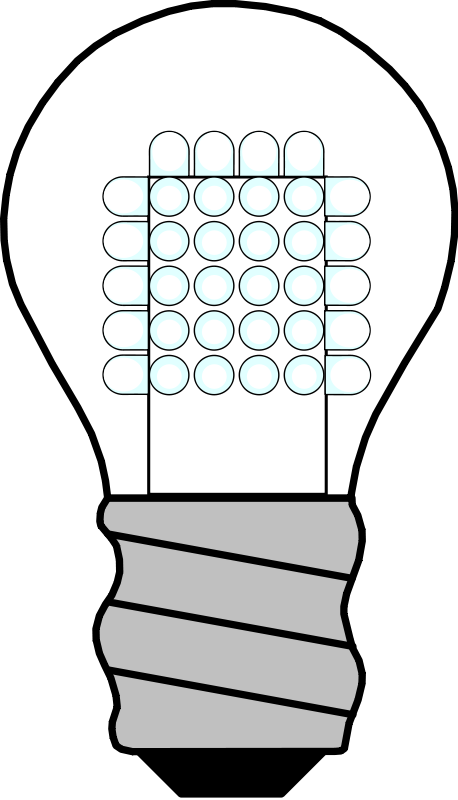
\includegraphics[scale=0.02]{imgs/bulb.png}
 \textbf{Nota} \\
 }%
{\endMakeFramed}

%Work in progress
\newenvironment{workinprogress}{%
  \def\FrameCommand{\colorbox{pink}}%
  \MakeFramed {\FrameRestore}
\lhdbend  \textbf{Work in progress} \\
 }%
{\endMakeFramed}

%Openquestion
\newenvironment{openquestion}{%
  \def\FrameCommand{\colorbox{pink}}%
  \MakeFramed {\FrameRestore}
 \textbf{Domanda aperta} \\
 }%
{\endMakeFramed}

%TODO
\newenvironment{todo}{%
  \def\FrameCommand{\colorbox{pink}}%
  \MakeFramed {\FrameRestore}
 \textbf{TODO} \\
 }%
{\endMakeFramed}

%%%%%%%%%%%%%%%%%%%%%%%%%%%%%%%%
%%%%%%%%%%%% HEADER %%%%%%%%%%%%
%%%%%%%%%%%%%%%%%%%%%%%%%%%%%%%%
\pagestyle{fancy}
% i comandi seguenti impediscono la scrittura in maiuscolo
% dei nomi dei capitoli e dei paragrafi nelle intestazioni
\renewcommand{\chaptermark}[1]{\markboth{#1}{}}
\renewcommand{\sectionmark}[1]{\markright{\thesection\ #1}}
\fancyhf{} % rimuove l'attuale contenuto dell'intestazione
% e del pi\`e di pagina
\fancyhead[LE,RO]{\bfseries\thepage}
\fancyhead[LO]{\bfseries\rightmark}
\fancyhead[RE]{\bfseries\leftmark}
\renewcommand{\headrulewidth}{0.5pt}
\renewcommand{\footrulewidth}{0pt}
\addtolength{\headheight}{0.5pt} % riserva spazio per la linea
\fancypagestyle{plain}{%
\fancyhead{} % ignora, nello stile plain, le intestazioni
\renewcommand{\headrulewidth}{0pt} % e la linea
}


%%%%%%%%%%%%%%%%%%%%%%%%%%%%%%%%
%%%%%%%%%%%% COLORS %%%%%%%%%%%%
%%%%%%%%%%%%%%%%%%%%%%%%%%%%%%%%
\definecolor{code}{gray}{0.3}


%%%%%%%%%%%%%%%%%%%%%%%%%%%%%%%%
%%%%%%%%%%%% NUMBERS %%%%%%%%%%%
%%%%%%%%%%%%%%%%%%%%%%%%%%%%%%%%
\setcounter{tocdepth}{3}
\setcounter{secnumdepth}{3}


%%%%%%%%%%%%%%%%%%%%%%%%%%%%%%%%
%%%%%%%%%%% DOC DATA %%%%%%%%%%%
%%%%%%%%%%%%%%%%%%%%%%%%%%%%%%%%
\title{Appunti di MNO}
\author{Gruppo Informatici Rampanti}
\date{ott 2010 - mag 2011}

\pdfinfo{%
  /Title    (Appunti di MNO)
  /Author   (Andrea Cimino e Lorenzo Muti)
  /Creator  (Andrea Cimino)
  /Producer (Lorenzo Muti)
  /Subject  (MNO)
  /Keywords (MNO)
}


%%%%%%%%%%%%%%%%%%%%%%%%%%%%%%%%
%%%%%%%%%%%%% UTILS %%%%%%%%%%%%
%%%%%%%%%%%%%%%%%%%%%%%%%%%%%%%%
% binary symbols
\newcommand{\modder}{\vdash _{R}}

% vertical gaps
\newcommand{\askip}{\vspace{0.5cm}}
\newcommand{\bskip}{\vspace{1.0cm}}

% various symbols
\newcommand{\qedhere}{\ensuremath{\Box}}
\newcommand{\qed}{\hfill \ensuremath{\Box}}

% substitution
\newcommand{\subst}[2]{^{#1} / _{#2}}

% denotational semantics function names
\newcommand{\bbracket}[1]{\left\llbracket #1 \right\rrbracket}

\newcommand{\aexpr}{\mathcal{A}}
\newcommand{\bexpr}{\mathcal{B}}
\newcommand{\cexpr}{\mathcal{C}}
\newcommand{\Aexpr}[1]{\mathcal{A} \bbracket{#1}}
\newcommand{\Bexpr}[1]{\mathcal{B} \bbracket{#1}}
\newcommand{\Cexpr}[1]{\mathcal{C} \bbracket{#1}}

\newcommand{\semdomset}[1]{(V_{#1})_{\bot}}

% semantic evaluations
\newcommand{\opereval}[3]{\left\langle #1, #2 \right\rangle \rightarrow #3}
\newcommand{\denaeval}[3]{\Aexpr{#1} #2 = #3}
\newcommand{\denbeval}[3]{\Bexpr{#1} #2 = #3}
\newcommand{\denceval}[3]{\Cexpr{#1} #2 = #3}

% rotated sqsubseteqs
\newcommand{\upsqsubseteq}{ $\begin{rotate}{90} $\sqsubseteq$ \end{rotate}$ }
\newcommand{\downsqsubseteq}{ $\begin{rotate}{270} $\sqsubseteq$ \end{rotate}$ }

% Space after paragraph declaration
\makeatletter
\renewcommand\paragraph{\@startsection{paragraph}{4}{\z@}%
  {-3.25ex\@plus -1ex \@minus -.2ex}%
  {1.5ex \@plus .2ex}%
  {\normalfont\normalsize\bfseries}}
\makeatother



% fast theorem and definition
\newcommand{\ftheo}[1]{\colorbox{YellowGreen}{#1}}
\newcommand{\fdefn}[1]{\colorbox{SkyBlue}{#1}}

\theoremstyle{break}
\theoremsymbol{\ensuremath{\clubsuit}}
\theoremseparator{\newline}
\newshadedtheorem{proc}[theo]{Procedura}

% bold math!
\newcommand{\bm}[1]{\mbox{\boldmath{$#1$}}}

\newcommand{\positive}[1]{\textbf{\color{green} +} #1}
\newcommand{\negative}[1]{\textbf{\color{red} -} #1}


\newtheoremlisttype{tab}%
{\begin{tabular*}{\linewidth}{@{}lrl@{\extracolsep{\fill}}r@{}}}%
{##1&##2&##3&##4\\}%
{\end{tabular*}}
\begin{document}
}
\providecommand{\outbpdocument}{\end{document}}
\else
\providecommand{\inbpdocument}{}
\providecommand{\outbpdocument}{}
\fi



\inbpdocument 

\chapter{Metodi di risoluzione per sistemi non lineari}
Andremo adesso a vedere come si possono risolvere i sistemi non
lineari. Per prima cosa caratterizziamoli.

Possiamo definire un sistema non lineare in due maniere: dato $ \Omega
\subseteq \Rset^n $, con $\Omega$ sotto insieme aperto di $\mathbb{R}^{n}$:

\begin{itemize}
\item $ F(\mathbf{x}) = \mathbf{0} \qquad \text{dove } F:\Omega \rightarrow \Rset^n $,
  dove
\[ F(\mathbf{x}) = \left\lbrace \begin{array}{c}
f_1(\mathbf{x}) = 0 \\ f_2(\mathbf{x}) = 0 \\ \vdots \\ f_n(\mathbf{x}) = 0
\end{array}  \right. \]
Le $f_i$ sono quindi funzioni del tipo $\Omega \rightarrow \mathbb{R}$.
\item $ \mathbf{x} = G(\mathbf{x}) \qquad \text{dove } G:\Omega \rightarrow \Rset^n $,
  ovvero
\[ \left\lbrace \begin{array}{c}
x_1 = g_1(\mathbf{x}) \\ 
x_2 = g_2(\mathbf{x}) \\ 
\vdots \\ 
x_n = g_n(\mathbf{x})
\end{array}  \right. \]
Anche le $g_i$ sono quindi funzioni del tipo $\Omega \rightarrow \mathbb{R}$.

\end{itemize}

Inoltre, se $ F(\mathbf{x}),G(\mathbf{x}) \in C^1(\Omega) $, le due funzioni generano le matrici Jacobiane, che chiameremo rispettivamente $ J(\mathbf{x}) $ ed $ H(\mathbf{x})$.

Per arricchire le possibilit\`a di personalizzare il metodo
risolutivo, possiamo porre
 $$ \mathbf{x} = G(\mathbf{x}) = \mathbf{x} - A(\mathbf{x})F(\mathbf{x})$$
per qualche $A(x)$.

Tale relazione si verifica in quanto $F(\mathbf{x}) = \mathbf{0}$ nella soluzione.


\section{Generalit\`a sui metodi iterativi per sistemi non lineari}
Possiamo dunque studiare le propriet\`a generali della famiglia dei
metodi iterativi che seguono lo schema

$$ x^{(i+1)} = G(x^{(i)}) = x^{(i)} - A(x^{(i)})F(x^{(i)}) $$

e che definiscono una successione di $ \mathbf{x}^{(i)} \in \Rset^n $ che
converge ad $ \alpha $ se $ \lim_{i \to \infty} || \mathbf{x}^{(i)}-\alpha
|| = 0 $

Vediamo adesso di capire se e quando questo schema iterativo pu\`o
convergere alla soluzione. Enunciamo un teorema che ci da una
condizione sufficiente per lo schema iterativo $ \mathbf{x}^{(i+1)} =
G(\mathbf{x}^{(i)}) $.

\begin{theo}[Teorema del punto fisso (sufficiente)]
Sia $ \mathbf{x} = G(\mathbf{x}) $ un sistema non lineare, e $ \alpha $ una soluzione di
tale sistema (tale dunque che $ \alpha = G(\mathbf{\alpha}) $). Sia $S$ un
intorno di $ \mathbf{\alpha} $, tale cio\'e che per un certo valore di $ \rho >
0 $ vale
\[ S = \left\lbrace x \in \Rset^n. || \mathbf{x} - \mathbf{\alpha} ||_{\infty} \leq \rho \right\rbrace \]
Sia inoltre
\[ \forall \mathbf{x} \in S.||H(\mathbf{x})||_{\infty} < 1 \]

Allora si ha convergenza per $ \mathbf{x}^{(0)} \in S $.
\end{theo}
\begin{thproof}
Per induzione si dimostra che
$$ || \mathbf{x}^{(i)} - \mathbf{\alpha} ||_{\infty} \leq \lambda^{i}\rho \quad
\text{dove } \lambda = \max_{S}||H(\mathbf{x})||_{\infty} $$

\begin{description}
\item[$ P(0) $] banalmente $ || \mathbf{x}^{(0)} - \alpha ||_{\infty} \leq 1
  \cdot \rho $ \`e  vera per ipotesi
\item[$ P(i) \Rightarrow P(i+1) $] So che $ \mathbf{x}^{(i)} - \mathbf{\alpha} =
  G(\mathbf{x}^{(i-1)}) - G(\alpha) $. Si tratta di un vettore: possiamo
  descrivere la $r$-esima componente, utilizzando il teorema del valor
  medio (\ref{teo-valor-medio-rn}), come
$$ \mathbf{x}^{(i)}_{r} - \alpha_{r} = g_r(\mathbf{x}^{(i-1)}) - g_r(\mathbf{\alpha}) =
 \nabla g_r (\mathbf{\xi}_r) ( \mathbf{x}^{(i-1)} - \mathbf{\alpha} )
 = \displaystyle \sum_{s=1}^{n} \dfrac{\partial g_r}{\partial x_s}(\xi_r)  (x_s^{(i-1)} - \alpha_s)
$$
e
$ \triangledown g_r (\mathbf{\xi}_r) $ \`e la riga $r$-esima della matrice
jacobiana di $G$ calcolata in $ \mathbf{\xi}_r $. Passiamo al modulo:
$$| x_r^{(i)} - \alpha_r | = \left| \displaystyle \sum_{s=1}^{n} \dfrac{\partial g_r}{\partial x_s}(\xi_r)  (x_s^{(i-1)} - \alpha_s) \right| $$
Per la disuguaglianza triangolare tra moduli (\ref{disuguaglianza-triangolare-moduli} a pag. \pageref{disuguaglianza-triangolare-moduli}) si ha:
$$ \left| \displaystyle \sum_{s=1}^{n} \dfrac{\partial g_r}{\partial x_s}(\xi_r)  (x_s^{(i-1)} - \alpha_s) \right| \leq 
\displaystyle \sum_{s=1}^{n} \left|\dfrac{\partial g_r}{\partial x_s}(\xi_r) (x_s^{(i-1)} - \alpha_s) \right| $$
Ricordando che $|ab|=|a|\cdot|b|$, si ha infine
$$| x_r^{(i)} - \alpha_r | \leq \sum^{n}_{s = 1} \left| \dfrac{\partial g_r}{\partial x_s}(\xi_r) \right| \left| x^{(i-1)}_s - \alpha_s \right| $$
Considerando che la norma infinito di un vettore è $|| y ||_{\infty} = \displaystyle \max_{i=1 \cdots n}|y_i|$, si ha
$$\sum^{n}_{s = 1} \left(\left| \dfrac{\partial g_r}{\partial x_s}(\xi_r) \right| \left| x^{(i-1)}_s - \alpha_s \right|\right)
\leq \sum^{n}_{s = 1} \left(\left| \dfrac{\partial g_r}{\partial x_s}(\xi_r) \right| || x^{(i-1)} - \alpha ||_{\infty} \right)
= \sum^{n}_{s = 1} \left(\left| \dfrac{\partial g_r}{\partial x_s}(\xi_r) \right| \right) || x^{(i-1)} - \alpha ||_{\infty}$$

Inoltre, considerando che la norma infinito di una matrice è $|| A ||_{\infty} = \displaystyle \max_{i=1 \cdots n}\sum_{j=1}^n|A_{ij}|$, e quindi $$|| H(x) ||_{\infty}  = \displaystyle \max_{i=1 \cdots n}\displaystyle \sum_{s=1}^{n}\left|\frac{\partial g_i(x)}{\partial x_s}\right|$$ si ha
\[
 \sum^{n}_{s = 1} \left(\left| \dfrac{\partial g_r}{\partial x_s}(\xi_r) \right| \right) || x^{(i-1)} - \alpha ||_{\infty} \leq || H(\xi_r) ||_{\infty}  || \mathbf{x}^{(i-1)} - \mathbf{\alpha} ||_{\infty} \leq \lambda || \mathbf{x}^{(i-1)} - \mathbf{\alpha} ||_{\infty} \]
In definitiva sappiamo che
\[ | x_r^{(i)} - \alpha_r | \leq \lambda || \mathbf{x}^{(i-1)} - 
\mathbf{\alpha} ||_{\infty} \quad r=1 \ldots n \]
questo vale in particolare per $r$ che massimizza  $| x_r^{(i)} - \alpha_r | $
\[ || \mathbf{x}^{(i)} - \mathbf{\alpha} ||_{\infty} \leq \lambda || \mathbf{x}^{(i-1)} - \mathbf{\alpha} ||_{\infty} \]
Possiamo quindi scrivere
\[ || \mathbf{x}^{(i)} - \mathbf{\alpha} ||_{\infty} \leq \lambda || \mathbf{x}^{(i-1)} - \alpha ||_{\infty} \leq \lambda^2 || \mathbf{x}^{(i-2)} - \mathbf{\alpha} ||_{\infty} \leq \ldots \leq \lambda^{(i)} || \mathbf{x}^{(0)} - \mathbf{\alpha} ||_{\infty} \leq \lambda^i \rho \]
in quanto $ \mathbf{x}^{(0)} \in S \Rightarrow ||\mathbf{x}^{(0)} - \mathbf{\alpha} ||_{\infty}
\leq \rho $.
\end{description}

Detto questo, \`e facile vedere che, essendo $ \lambda < 1 $, $
\lambda^i \rho \xrightarrow{i \rightarrow \infty} 0 $ e che quindi $
|| \mathbf{x}^{(i)} - \mathbf{\alpha} ||_{\infty} \xrightarrow{i \rightarrow \infty} 0 $
\end{thproof}

Questo teorema fornisce una condizione sufficiente per la
convergenza. Se quindi si verificano le ipotesi, possiamo affermare
con certezza che il metodo converge. Ma il metodo pu\`o convergere
anche se le condizioni non si verificano!

Vediamo un esempio.

\begin{example}
Consideriamo il sistema non lineare
 $$ \left\{
\begin{array}{l}
 x_1 = g_1(x) = \frac{1}{4}(x_{1}^{2} + x_{2}^{2}) \\ x_2 = g_2(x) =
 \sin(x_1 + 1)
\end{array}
\right. \qquad x= \begin{pmatrix} x_1 \\ x_2
    \end{pmatrix}
$$

Vogliamo

\begin{itemize}
 \item Verificare l'esistenza di punti fissi
 \item Applicare il teorema del punto fisso
\end{itemize}

Tracciamo il grafico delle due funzioni. La prima delle due \`e una
circonferenza, la seconda un seno.

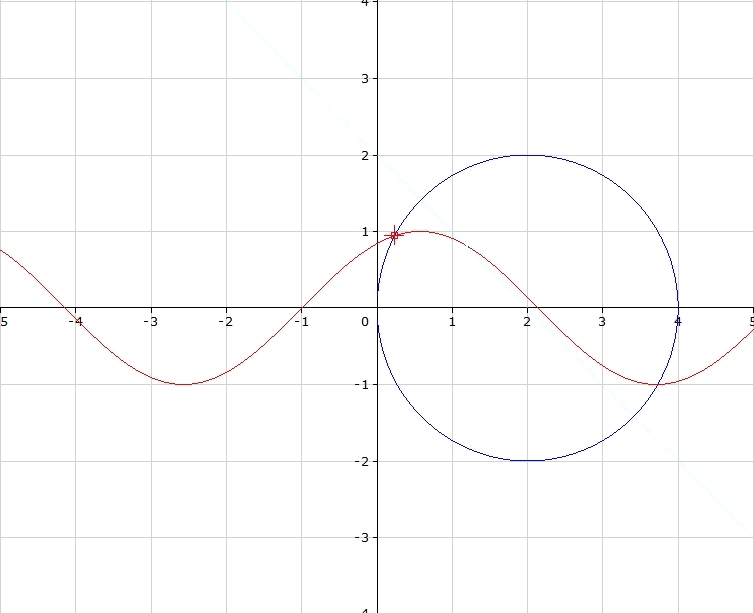
\includegraphics[width=350px]{imgs/121701.jpg}

Come possiamo vedere, ci sono due punti di incontro, che chiameremo $
\alpha $ (quello pi\`u vicino all'asse delle ordinate) e $ \beta
$. Ora devo trovare un intorno S di uno dei due punti tale che $
\forall x \in S.||H(x)||_{\infty} < 1 $. Calcoliamo $ H(x) $, che
ricordiamo essere la matrice la quale, sulle righe, ha i gradienti
delle funzioni che compongono $G$.

$$ H(x) = \left[\begin{array}{cc} \frac{x_1}{2} & \frac{x_2}{2}
    \\ \cos(x_1 +1)& 0
\end{array}          
\right]
$$

Devo ora calcolare la norma infinito della matrice, lasciando $x$
parametrico. La norma infinito \`e la massima somma degli elementi
delle righe di

$$ ||H(x) ||_{\infty} = \max(\frac{1}{2} (|x_{1}| + |x_{2}|), |
cos(x_1 + 1)|) $$

Voglio che $ || H(x) ||_{\infty} $ sia minore di 1: ovviamente $ |
cos(x_1 + 1)| < 1 $, quindi rimane da vedere che $ \frac{1}{2}
(|x_{1}| + |x_{2}|) < 1 $. Questo accade quando $ x_1 + x_2 < 2
$. Possiamo dunque tracciare l'equazione della retta $ y = - x + 2 $
sotto la quale vale sempre $ || H(x) || _{\infty} < 1 $. Possiamo
vedere il grafico di questa retta nella pagina successiva.

Se prendiamo $ \alpha $, appare evidente che possiamo costruirne un
intorno S non vuoto tale che $ \forall x \in S.H(x) < 1 $: basta che
tale intorno non oltrepassi la retta $ x_1 + x_2 < 2 $. Non possiamo
dire la stessa cosa per $ \beta $: infatti $ H(\beta) > 1 $ ed \`e
quindi impossibile costruirne un intorno in cui la propriet\`a non
vada. Ma pu\`o darsi che il metodo funzioni comunque, in quanto la
propriet\`a enunciata \emph{non \`e necessaria}.

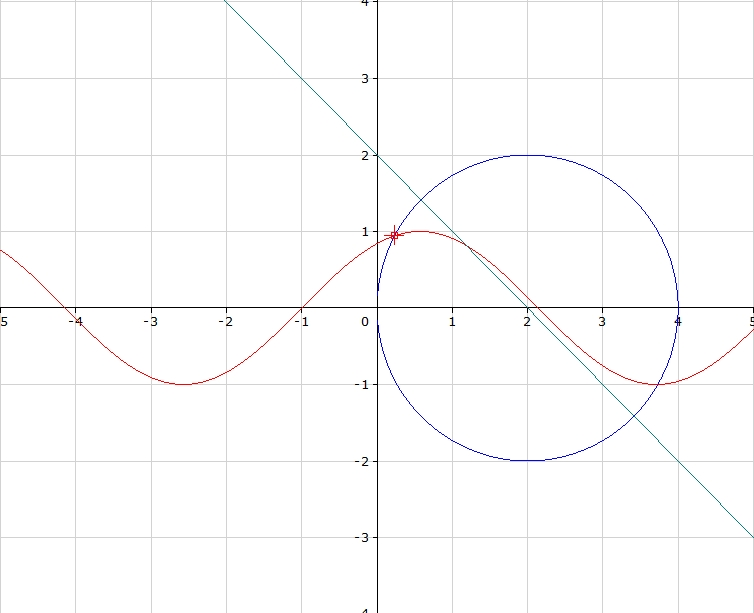
\includegraphics[width=350px]{imgs/121702.jpg}
\end{example}

Enunciamo un secondo teorema del punto fisso, che \`e  necessario e
sufficiente.

\begin{theo}[Teorema del punto fisso (necessario e sufficiente)]\label{theo:ptofisso2}
Siano
\begin{itemize}
\item $g(\mathbf{x})$ di classe $C^{1}(\Omega)$
\item $\Omega$ insieme aperto
\item $ \mathbf{\alpha} $ punto di $ \Omega $ tale che $ \mathbf{\alpha} = g(\mathbf{\alpha}) $
  ($ \mathbf{\alpha} $ \`e punto fisso di $g$)
\end{itemize}
Allora esiste una norma $|| \cdot ||_* $ vettoriale ed un intorno $ S
= \left\lbrace x : || x - \alpha ||_* < \pi \right\rbrace $ tale che
per $\mathbf{x}^{(0)}\in S$ si ha convergenza se e solo se $\rho(H(\mathbf{\alpha}))
\leq 1$.
\end{theo}

Non dimostreremo questo teorema. Piuttosto viene da chiedersi il
perch\'e delle differenze fra i due teoremi: uno pone condizioni sulla
norma, l'altro sul raggio spettrale.

Effettivamente esiste un legame fra queste due grandezze: si veda il Teorema \ref{th:raggio-spettrale-norme-indotte} a pagina \pageref{th:raggio-spettrale-norme-indotte}, il quale asserisce che per ogni matrice $B$ e per ogni norma indotta $|| \cdot ||$ vale
$$ \rho(B) = \inf_{|| \cdot || \text{ indotta}}\{ ||B||\}$$

In particolare, se $ \rho(B) < 1 $, possiamo trovare, prendendo $
\varepsilon < 1 - || H(\alpha) || $, una norma $ ||\cdot||_* $ tale che

$$ \rho(B) \leq || B||_* \leq \rho(B) + \varepsilon$$

verificando dunque la condizione del teorema del punto fisso nella sua
versione sufficiente, in quanto per la continuit\`a di $g$ esister\`a un
intorno di $ \mathbf{\alpha} $ nel quale la matrice hessiana avr\`a norma
minore di 1.


\section{Metodo di Newton-Raphson (delle tangenti)}
\label{section:metodo-newton-raphson}
Vediamo adesso un metodo per la risoluzione di sistemi non
lineari che segue lo schema presentato nel paragrafo precedente: il metodo di Newton-Raphson. Si tratta di un'estensione del
metodo di Newton.

Prendiamo il nostro problema, espresso al solito nelle due forme
alternative $ F(\mathbf{x}) = \mathbf{0} $ e 
$ \mathbf{x} = G(\mathbf{x}) $. Abbiamo visto che possiamo
sempre ottenere da tali espressioni la relazione

\[ \mathbf{x} = G(\mathbf{x}) = \mathbf{x} -
A(\mathbf{x})F(\mathbf{x}) \]

per una qualche funzione $A(\mathbf{x})$. Il metodo di Newton-Raphson prende $A(\mathbf{x}) = J^{-1}(\mathbf{x}) $, dove 
$J(\mathbf{x})$ \`e la matrice Jacobiana di $F$. Manipolando
otteniamo che

\[ \mathbf{x}^{(i+1)} = \mathbf{x}^{(i)} - J^{-1}(\mathbf{x}^{(i)})F(\mathbf{x}^{(i)}) \quad \Rightarrow \quad J(\mathbf{x}^{(i)})(\mathbf{x}^{(i+1)} - \mathbf{x}^{(i)}) = - F(\mathbf{x}^{(i)}) \]

che \`e un sistema lineare che ha $ J(\mathbf{x}^{(i)}) $ come matrice dei
coefficienti, $ \mathbf{x}^{(i+1)} - \mathbf{x}^{(i)} $ come incognite e $ - F(\mathbf{x}^{(i)})$ come vettore dei termini noti.

\begin{example}[Matrice associata al metodo di Newton-Raphson]
Nel caso delle matrici 2x2 ottengo il sistema
$$ \left[
\begin{array}{cc}
\frac{\partial f_1}{\partial x_1}(x^{(i)}) & \frac{\partial
  f_1}{\partial x_2}(x^{(i)}) \\ \frac{\partial f_2}{\partial
  x_1}(x^{(i)}) & \frac{\partial f_2}{\partial x_2}(x^{(i)})
\end{array} 
\right] \left[
\begin{array}{c}
\theta_1 \\ \theta_2
\end{array} 
\right] = \left[
\begin{array}{c}
 - f_1(x^{(i)}) \\ -f_2(x^{(i)}) \\
\end{array} 
\right]
$$

dove $ \theta = x^{(i+1)} - x^{(i)} $
\end{example}

Al solito, dobbiamo dimostrare che il metodo converge.

\begin{theo}[Convergenza di Newton-Raphson]
\label{theo:convergenza-newton-raphson}
Siano
\begin{itemize}
\item $ F(\mathbf{x}) \in C^2(\Omega) $ con matrice jacobiana $ J(\mathbf{x}) $
\item $ \mathbf{\alpha} \in \Omega $ tale che $ F(\mathbf{\alpha}) =\mathbf{0} $
\end{itemize}
Allora, se $ J(\mathbf{x}) $ \`e non singolare in $ \Omega $, $ \exists S
\subseteq \Omega $ intorno di $ \mathbf{\alpha} $ tale che, preso $ \mathbf{x}^{(0)} \in
S $:
\begin{enumerate}[(a)]
\item la successione $ \left\lbrace \mathbf{x}^{(i)} \right\rbrace_{i} $
  generata dal metodo di Newton-Raphson a partire dal punto
 $ \mathbf{x}^{(0)}$ converge a $ \mathbf{\alpha} $
\item $ \forall || \cdot ||.\exists \beta.\forall i > 0.|| \mathbf{x}^{(i+1)} -
  \mathbf{\alpha} || \leq \beta || \mathbf{x}^{(i)} - \mathbf{\alpha} ||^2 $
\end{enumerate}
\end{theo}

\begin{thproof}
Dimostriamo i due punti del teorema.

\begin{enumerate}[(a)]
\item Per comodit\`a di notazione nella dimostrazione scriveremo $
  K(\mathbf{x}) = J^{-1}(\mathbf{x}) $. Abbiamo dunque

\[ G(\mathbf{x}) = \mathbf{x} - K(\mathbf{x})F(\mathbf{x}) \]

Si tratta di un'uguaglianza fra vettori: prendiamone la $r$-esima
componente.

\[ g_r(\mathbf{x}) = x_r - \sum_{s=1}^{n}K_{rs}(\mathbf{x})f_{s}(\mathbf{x}) \]

Deriviamo rispetto ad $ x_t $, per $ t \in [1,n] $, ottenendo i valori
della matrice jacobiana $H$ di $g$.

\[ h_{rt}(\mathbf{x}) = \dfrac{\partial g_r}{\partial x_t}(\mathbf{x}) =
\delta_{rt} - \sum_{s=1}^{n} \dfrac{\partial K_{rs}}{\partial x_t}(\mathbf{x})
f_s(\mathbf{x}) - \sum_{s=1}^{n} K_{rs}(\mathbf{x}) \dfrac{\partial f_s}{\partial
  x_t}(\mathbf{x})\]

dove $ \delta_{rt} $ vale 1 se $ r=t $ e $0$ altrimenti. Analizziamo il
terzo addendo: si tratta del prodotto fra la r$-$esima riga di K (ovvero
la $r$-esima riga di $ J^{-1} $) e la $t$-esima colonna di $J$. Visto che $
JJ^{-1} = I $ per definizione di matrice inversa, so che tale prodotto
deve fare $1$ se $ r=t $ e $0$ altrimenti. Ho quindi che $ \delta_{rt} =
\displaystyle \sum_{s=1}^{n} K_{rs}(\mathbf{x}) \dfrac{\partial f_s}{\partial x_t}(\mathbf{x})$, e
posso annullarli uno con l'altro. Rimane dunque

\[ h_{rt}(\mathbf{x}) = - \sum_{s=1}^{n} \dfrac{\partial K_{rs}}{\partial x_t}(\mathbf{x}) f_s(\mathbf{x}) \]

che implica che $ h_{rt}(\mathbf{\alpha}) = 0 $, in quanto $ \forall
s.f_s(\alpha) = 0 $. Quindi $ \rho (H(\mathbf{\alpha})) = 0 $, e posso
applicare il teorema \ref{theo:ptofisso2} del punto fisso che mi
assicura la convergenza in un intorno $S$ di $ \mathbf{\alpha} $.
\item Vale
\[ J(x^{(i)})(x^{(i+1)} - x^{(i)}) = - F(x^{(i)}) \]
\[ J(x^{(i)})\left[ (x^{(i+1)} - \alpha) - (x^{(i)} - \alpha) \right] = - F(x^{(i)}) \]
\begin{equation} 
J(x^{(i)}) (x^{(i+1)} - \alpha) = J(x^{(i)}) (x^{(i)} - \alpha) -
F(x^{(i)})
\label{eqn:newtrhap1}\end{equation}

Indichiamo con $ S_r $ le matrici hessiane delle funzioni $ f_r $.

\[ (S_r(x))_{st} = \dfrac{\partial^2 f_r}{\partial x_s \partial x_t} (x) \]

Applicando la sostituzione di Taylor posso porre

\[ F(\alpha) = F(x^{(i)}) + J(x^{(i)})(\alpha - x^{(i)}) + v \]
\begin{equation}
-F(x^{(i)}) = - F(\alpha) + J(x^{(i)})(\alpha - x^{(i)}) + v
\label{eqn:newtrhap3}\end{equation}

dove $ v = \frac{1}{2} (x^{(i)} - \alpha)^T S_r (\xi_r)(x^{(i)} -
\alpha) $, e passando a moduli e norme,

\begin{equation}
|v_r| \leq \frac{n}{2} || S_r(\xi_r) ||_{\infty} || x^{(i)}-\alpha
||_{\infty}^2
\label{eqn:newtrhap4}\end{equation}

Abbiamo tutti i pezzi per trarre la conclusione: prendiamo l'equazione
\ref{eqn:newtrhap1} ed applichiamo la sostituzione
\ref{eqn:newtrhap3}:

\[ J(x^{(i)}) (x^{(i+1)} - \alpha) = J(x^{(i)}) (x^{(i)} - \alpha) - F(x^{(i)}) \]
\[ J(x^{(i)}) (x^{(i+1)} - \alpha) = J(x^{(i)}) (x^{(i)} - \alpha) - F(\alpha) + J(x^{(i)})(\alpha - x^{(i)}) + v \]

Essendo $ F(\alpha) = 0 $ e $ (x^{(i)} - \alpha) = - (\alpha -
x^{(i)}) $, ottengo $ (x^{(i+1)} - \alpha) = J^{-1}(x^{(i)}) v
$. Passando alle norme ed applicando \ref{eqn:newtrhap4} ottengo

\[ ||x^{(i+1)} - \alpha ||_{\infty} \leq \gamma || x^{(i)} - \alpha ||_{\infty}^2 \]

per $ \gamma = \frac{n}{2} \max _{x \in S} || K(x) ||_{\infty} \max_{x
  \in S, r \in [1,n]} ||S_r(x)|| _{\infty} $

Notare che $ \gamma $ \`e costante: per l'equivalenza topologica fra
le norme, esister\'a un $ \beta $ per cui questa relazione vale per
qualunque norma $ || \cdot || $, come volevasi dimostrare.
\end{enumerate}
\end{thproof}


%%Buco dell`ultima lezione prima di Natale (Newton Raphson)

%%% Local Variables: 
%%% mode: latex
%%% TeX-master: "appunti"
%%% End: 

\subsection{Newton-Raphson su funzioni convesse}
Per via delle proprietà delle funzioni convesse, possiamo utilizzare Newton-Raphson con risultati di convergenza sensibilmente migliori rispetto al normale. Otterremo questo risultato grazie ai due teoremi seguenti.

Il primo teorema lega le proprietà della matrice Jacobiana alla convessità.

\begin{theo}[Legame fra matrice Jacobiana e convessità]\label{theo:legamejacobconvessita}
Siano
\begin{itemize}
\item D insieme convesso
\item $ f \in C^1(D) $
\end{itemize}
Allora f \`e  convessa su D \textbf{se e solo se} $ f(v) - f(u) \geq J(u)(v-u) $ 
\end{theo}
\begin{thproof}
Dimostriamo i due sensi della doppia implicazione

\begin{description}
\item[$ \Leftarrow $] Assumiamo $ f(v) - f(u) \geq J(u)(v-u) $. Siano
\begin{itemize}
\item $ x,y \in D $
\item $ \lambda \in [0,1] $
\item $ z(\lambda) = \lambda \cdot x + (1-\lambda ) \cdot y $
\end{itemize}

Ovviamente, essendo D convesso, avremo che $ z(\lambda) \in D $ per definizione di insieme convesso.  Possiamo dire che

\begin{eqnarray*}
f(x) - f(z(\lambda)) \geq J(z(\lambda)) (x -z(\lambda)) \\
f(y) - f(z(\lambda)) \geq J(z(\lambda)) (y -z(\lambda))
\end{eqnarray*}

Moltiplichiamo la prima equazione per $ \lambda $ e la seconda per $ (1 - \lambda) $, e sommiamo membro a membro. Otterremo

\[ \lambda f(x) + (1 - \lambda) f(y) - f(z(\lambda)) \geq J(z(\lambda))(\lambda x + (1 - \lambda) y - z(\lambda))  \]

Ma 

\[ \lambda x + (1 - \lambda) y - z(\lambda) = \lambda x + (1 - \lambda) y - \lambda x - (1 - \lambda) y = 0 \]

La parte destra \`e  dunque uguale a zero: rimane la relazione

\[ \lambda f(x) + (1 - \lambda) f(y) \geq f(z(\lambda)) = f(\lambda x + (1-\lambda ) \cdot y) \]

che corriponde alla definizione di funzione convessa vista in \ref{richiamibigi:funzioneconvessa} a pagina \pageref{richiamibigi:funzioneconvessa}.

\item[$ \Rightarrow $] Supponiamo adesso che f sia convessa in D. Siano
\begin{itemize}
\item $ u,v \in D $
\item $ \lambda \in [0,1] $
\item $ w(\lambda) = \lambda v + (1 - \lambda) u $
\end{itemize}

Essendo $ f \in C^1(D) $, per una qualunque norma $ ||\cdot || $ esiste il \emph{differenziale totale}
\[ \lim_{x' \rightarrow x} \dfrac{|| f(x') - f(x) - J(x)(x' - x) ||}{|| x' - x ||} = 0 \]

Preso $ x' = w(\lambda), x = u $ ho, considerando che $ || w(\lambda) - u || = || \lambda v + (1 - \lambda) u - u || = || \lambda v - \lambda u || = |\lambda| || v - u || $ e che $ w(\lambda) \rightarrow u \Leftrightarrow \lambda \rightarrow 0 $,

\[ \lim_{\lambda \rightarrow 0} \dfrac{|| f(w(\lambda)) - f(u) - J(u)(w(\lambda) - u) ||}{|| w(\lambda) - u ||} = 0 \Leftrightarrow \]
\[ \Leftrightarrow \lim_{\lambda \rightarrow 0} \frac{1}{\lambda} || f(w(\lambda)) - f(u) - \lambda J(u)(v - u) || = 0 \Leftrightarrow \]
\[ \Leftrightarrow \lim_{\lambda \rightarrow 0} \frac{1}{\lambda} \left[ f(w(\lambda)) - f(u) \right] = J(u)(v - u) \]

Ma abbiamo che, per la definizione di funzione convessa,

\[ \lambda f(v) + (1 - \lambda)f(u) \geq f(w(\lambda)) \Leftrightarrow f(v) - f(u) \geq \frac{1}{\lambda} \left[ f(w(\lambda)) - f(u) \right] \]

e che quindi

\[ \lambda f(v) + (1 - \lambda)f(u) \geq J(u)(v - u) \]

come volevasi dimostrare
\end{description}
\end{thproof}

Detto questo, possiamo dimostrare che

\begin{theo}[Convergenza di Newton-Raphson per funzioni convesse]
Siano
\begin{itemize}
\item $ a_i, b_i \in \Rset^n, i \in [1,n] $
\item D intervallo di $ \Rset^n $
\item $ f \in C^1(D) $ convessa su D
\item $ \alpha \in D $ tale che $ f(\alpha) = 0 $
\end{itemize}

Allora, se si verificano le seguenti condizioni
\begin{itemize}
\item $ \forall x \in D. J(x) $ non \`e  singolare
\item $ [J(x)]^{-1} \geq 0 $
\end{itemize}
e considerata la successione $ \left\lbrace x^{(i)} \right\rbrace_i $ generata dal metodo di Newton-Raphson, vale la seguente relazione:
\[ \forall x^{(0)} \in D \text{ tale che } f(x^{(0)}) \geq 0 \; \lim_{i \to \infty} x^{(i)} \rightarrow \alpha \]

Inoltre $ \alpha $ \`e  l'unica soluzione del problema.
\end{theo}
\begin{thproof}
Per prima cosa dimostriamo per induzione su i che
\begin{itemize}
\item $ \forall i \quad \alpha \leq x^{(i+1)} \leq x^{(i)} $
\item $ f(x^{(i+1)}) \geq 0 $
\end{itemize}
Il secondo punto servir\'a solamente per applicare l'induzione. Il primo punto \`e  quello importante: ci dice che la successione di $ x^{(i)} $ si avvicina verso $ \alpha $.

\begin{description}
\item[Passo base] Dal teorema \ref{theo:legamejacobconvessita} sappiamo che, se f \`e  convessa, vale $ f(\alpha) - f(x^{(0)}) \geq J(x^{(0)})(\alpha - x^{(0)}) $, e che dunque

\begin{equation}
-[J(x)]^{-1}f(x^{(0)}) \geq \alpha - x^{(0)}
\label{eqn:nrfunzconv}
\end{equation}

Essendo $ [J(x^{(0)})]^{-1} \geq 0 $ e $ f(x^{(0)}) \geq 0 $ per ipotesi, ottengo

\begin{itemize}
\item $ \alpha \leq x^{(0)} $ in quanto $ \alpha - x^{(0)} $ \`e  un valore negativo
\item $ \alpha \leq x^{(1)} = x^{(0)}-[J(x)]^{-1}f(x^{(0)} \leq x^{(0)} $
\end{itemize}

Inoltre, sempre per il fatto che f \`e  convessa, posso applicare il teorema \ref{theo:legamejacobconvessita} ottenendo
\[ f(x^{(1)} - f(x^{(0)} \geq J(x^{(0)})(x^{(1)} - x^{(0)}) \]
Questa relazione, essendo $ J(x^{(0)})(x^{(1)} - x^{(0)}) = -f(x^{(0)}) $ per definizione del metodo, implica $ f(x^{(1)}) \geq 0 $. Inoltre, essendo $ x^{(1)} $ compreso fra $ x^{(0)} $ e $ \alpha $, abbiamo che $ x^{(1)} \in D $ e che quindi $ [J(x^{(1)})]^{-1} \geq 0 $

\item[Passo induttivo] Essendo $ [J(x^{(1)})]^{-1} \geq 0 $ e $ f(x^{(1)}) \geq 0 $ posso applicare esattamente la stessa dimostrazione vista per il passo base.
\end{description}

La successione \`e  quindi decrescente e inferiormente limitata: possiamo esser sicuri che converge ad un valore $ \beta $ per il quale
\[ f(\beta) = \lim_{i \rightarrow \infty} f(x^{(i)}) = \]
\[ = \lim_{i \rightarrow \infty} J(x^{(i)})\left[ x^{(i)} - x^{(i-1)} \right] = \]
\[ = \lim_{i \rightarrow \infty} J(x^{(i)})\left[ \beta - \beta \right] = 0 \]
Quindi $ \beta $ \`e  un'altra soluzione dell'equazione: ma dal teorema \ref{theo:legamejacobconvessita} posso concludere che
\[ 0 = f(\alpha) - f(\beta) \geq J(\alpha)(\beta - \alpha) \]
\[ 0 = f(\beta) - f(\alpha) \geq J(\beta)(\alpha - \beta) \]
ed essendo $ [J(\alpha)]^{-1} \geq 0, [J(\beta)]^{-1} \geq 0 $ ho
\[ \left. \begin{array}{c}
0 \geq \beta - \alpha \\ 
0 \geq \alpha - \beta
\end{array}  \right. \Rightarrow \alpha = \beta \]

Quindi, ricapitolando
\begin{itemize}
\item la successione converge ad un valore
\item tale valore \`e  $\alpha$, che \`e  soluzione \emph{unica}
\end{itemize}
\end{thproof}

\outbpdocument
 %% Bevi: risoluzione sistemi non lineari
 %% Copyright (C) 2011, Andrea Cimino, All Rights Reserved. 
 %% This file is distributed under the terms of the Creative Common
 %% Licence Non-Commercial Share-Alike license

%% 11 Gennaio 2011

 %% Useful stuff for separate compilation.
\ifx\ismaindoc\undefined
\providecommand{\inbpdocument}{
 \documentclass[11pt,a4paper,twoside,titlepage]{scrbook}
%%%%%%%%%%%%%%%%%%%%%%%%%%%%%%%%
%%%%%%%%%%% PACKAGES %%%%%%%%%%%
%%%%%%%%%%%%%%%%%%%%%%%%%%%%%%%%
% encoding
\usepackage[utf8x]{inputenc}
\usepackage[italian]{babel} % babel (suddivisione parole in sillabe)

\usepackage{amsfonts} % matematica
\usepackage{amsmath} % matematica
\usepackage{amssymb} % simboli vari
\usepackage{calrsfs}
\usepackage{caption}
\usepackage{enumerate}
\usepackage{extarrows} % matematica
\usepackage{keyval}
\usepackage{manfnt} % Simboli curva
\usepackage{mathtools} % matematica
\usepackage{multirow} 
\usepackage[usenames, dvipsnames]{color} % colori con nome
\usepackage[pdftex]{graphicx}
\usepackage{epstopdf} % gestione file EPS
\usepackage{wrapfig} % per figure circondate da testo
\usepackage{framed}	% teoremi framed
\usepackage{fancyhdr} % header buffi
\usepackage[T1]{fontenc} % gestione hbox e vbox
\usepackage[a4paper]{geometry}
\usepackage{microtype} % gestione hbox e vbox
\usepackage[thref, amsthm, amsmath, framed, hyperref]{ntheorem} % teoremi (avanzata)
%% \usepackage{prooftree} % gestione prof-tree
\usepackage{rotating}
\usepackage{stmaryrd}
\usepackage{subfig}
\usepackage{syntax} % syntattic stuff
\usepackage{txfonts}
\usepackage{verbatim} % migliorie al verbatim
%\usepackage{hyperref}
%% \usepackage{qtree}
\usepackage{fancyvrb}
\usepackage{listings}
\usepackage{cancel}
\usepackage{tikz}

\usepackage{bbding} %% Icons

%%%%%%%%%%%%%%%%%%%%%%%%%%%%%%%%
%%%%%%%%%%% GEOMETRY %%%%%%%%%%%
%%%%%%%%%%%%%%%%%%%%%%%%%%%%%%%%
\geometry{verbose,tmargin=2cm,bmargin=2.5cm,lmargin=2.5cm,rmargin=2cm}
\parindent0ex %% Remove paragraph indenting

%%%%%%%%%%%%%%%%%%%%%%%%%%%%%%%%
%%%%%%%%%%% CODE ENV %%%%%%%%%%%
%%%%%%%%%%%%%%%%%%%%%%%%%%%%%%%%
% codice
\newcounter{count}
\setcounter{count}{0}
\newenvironment{code}[1]
{
\color{lightgray}\hrulefill\color{code}
\stepcounter{count} {\bf\small Listato di codice \arabic{count}: {#1} }
\verbatim
}
{
\endverbatim
\color{lightgray}\hrulefill
\color{black}
\\
}

% codice semplice
\newenvironment{simplecode}
{
\color{code} \tt
}
{
\rm
}

 % Notation issues
\input{macros}

\makeatletter
\g@addto@macro\@verbatim\footnotesize
\makeatother



%%%%%%%%%%%%%%%%%%%%%%%%%%%%%%%%
%%%%%%%% THEOREMS FORMAT %%%%%%%
%%%%%%%%%%%%%%%%%%%%%%%%%%%%%%%%
% shaded theorems and proofs command
\definecolor{lightgray}{RGB}{230,230,230}
\def\theoremframecommand{\colorbox{lightgray}}

%%% theorems
\theoremstyle{break}
\theoremheaderfont{\normalfont\bfseries}
\theorembodyfont{\itshape}
\theoremsymbol{\ensuremath{\diamondsuit}}
\theoremseparator{\newline}
\newtheorem{theo}{
\includegraphics[scale=0.11]{imgs/book.png}Teorema}[chapter]

%%% propositions
\theoremstyle{break}
\theoremheaderfont{\normalfont\bfseries}
\theorembodyfont{\itshape}
\theoremsymbol{\ensuremath{\diamondsuit}}
\theoremseparator{\newline}
\newshadedtheorem{proposition}{Proposizione}[chapter]

%%% exercises
\theoremstyle{break}
\theoremheaderfont{\normalfont\bfseries}
\theorembodyfont{\itshape}
\theoremsymbol{\ensuremath{\diamondsuit}}
\theoremseparator{\newline}
\newshadedtheorem{exercise}{Esercizio}[chapter]

%%% propositions
\theoremstyle{break}
\theoremheaderfont{\normalfont\bfseries}
\theorembodyfont{\itshape}
\theoremsymbol{\ensuremath{\diamondsuit}}
\theoremseparator{\newline}
\newshadedtheorem{property}{\PencilRightDown $\; $ Propriet\`a}[chapter]

%%% lemmas
\theoremstyle{break}
\theoremheaderfont{\normalfont\bfseries}
\theorembodyfont{\itshape}
\theoremsymbol{\ensuremath{\diamondsuit}}
\theoremseparator{\newline}
\newshadedtheorem{lemma}[theo]{Lemma}

%%% definitions
\theoremstyle{break}
\theoremsymbol{\ensuremath{\clubsuit}}
\theoremseparator{\newline}
\newshadedtheorem{defn}[theo]{Definizione}

%%% examples
\theoremstyle{break}
\theorembodyfont{\itshape}
\theoremsymbol{\ensuremath{\ast}}
\theoremseparator{\newline}
\newshadedtheorem{example}[theo]{Esempio}

%%% observations
\theoremstyle{break}
\theorembodyfont{\itshape}
\theoremsymbol{\ensuremath{\ast}}
\theoremseparator{\newline}
\newshadedtheorem{observation}[theo]{

\includegraphics[scale=0.06]{imgs/lens.png}
Osservazione
}

%%% notations
\newtheorem*{notaz}{Notazione}

%%% proofs
\newenvironment{thproof}
{
\vskip 0.03cm
\begin{small}
\textit{Dimostrazione. }
\color{code}
}
{
\color{black}
\end{small}
$ \square $
\vskip 0.2cm
}

%Notes
\newenvironment{notes}{%
  \def\FrameCommand{\colorbox{yellow}}%
  \MakeFramed {\FrameRestore}
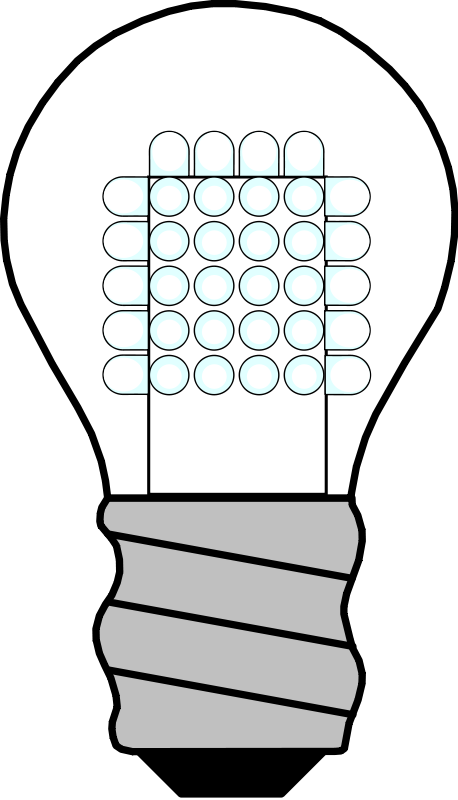
\includegraphics[scale=0.02]{imgs/bulb.png}
 \textbf{Nota} \\
 }%
{\endMakeFramed}

%Work in progress
\newenvironment{workinprogress}{%
  \def\FrameCommand{\colorbox{pink}}%
  \MakeFramed {\FrameRestore}
\lhdbend  \textbf{Work in progress} \\
 }%
{\endMakeFramed}

%Openquestion
\newenvironment{openquestion}{%
  \def\FrameCommand{\colorbox{pink}}%
  \MakeFramed {\FrameRestore}
 \textbf{Domanda aperta} \\
 }%
{\endMakeFramed}

%TODO
\newenvironment{todo}{%
  \def\FrameCommand{\colorbox{pink}}%
  \MakeFramed {\FrameRestore}
 \textbf{TODO} \\
 }%
{\endMakeFramed}

%%%%%%%%%%%%%%%%%%%%%%%%%%%%%%%%
%%%%%%%%%%%% HEADER %%%%%%%%%%%%
%%%%%%%%%%%%%%%%%%%%%%%%%%%%%%%%
\pagestyle{fancy}
% i comandi seguenti impediscono la scrittura in maiuscolo
% dei nomi dei capitoli e dei paragrafi nelle intestazioni
\renewcommand{\chaptermark}[1]{\markboth{#1}{}}
\renewcommand{\sectionmark}[1]{\markright{\thesection\ #1}}
\fancyhf{} % rimuove l'attuale contenuto dell'intestazione
% e del pi\`e di pagina
\fancyhead[LE,RO]{\bfseries\thepage}
\fancyhead[LO]{\bfseries\rightmark}
\fancyhead[RE]{\bfseries\leftmark}
\renewcommand{\headrulewidth}{0.5pt}
\renewcommand{\footrulewidth}{0pt}
\addtolength{\headheight}{0.5pt} % riserva spazio per la linea
\fancypagestyle{plain}{%
\fancyhead{} % ignora, nello stile plain, le intestazioni
\renewcommand{\headrulewidth}{0pt} % e la linea
}


%%%%%%%%%%%%%%%%%%%%%%%%%%%%%%%%
%%%%%%%%%%%% COLORS %%%%%%%%%%%%
%%%%%%%%%%%%%%%%%%%%%%%%%%%%%%%%
\definecolor{code}{gray}{0.3}


%%%%%%%%%%%%%%%%%%%%%%%%%%%%%%%%
%%%%%%%%%%%% NUMBERS %%%%%%%%%%%
%%%%%%%%%%%%%%%%%%%%%%%%%%%%%%%%
\setcounter{tocdepth}{3}
\setcounter{secnumdepth}{3}


%%%%%%%%%%%%%%%%%%%%%%%%%%%%%%%%
%%%%%%%%%%% DOC DATA %%%%%%%%%%%
%%%%%%%%%%%%%%%%%%%%%%%%%%%%%%%%
\title{Appunti di MNO}
\author{Gruppo Informatici Rampanti}
\date{ott 2010 - mag 2011}

\pdfinfo{%
  /Title    (Appunti di MNO)
  /Author   (Andrea Cimino e Lorenzo Muti)
  /Creator  (Andrea Cimino)
  /Producer (Lorenzo Muti)
  /Subject  (MNO)
  /Keywords (MNO)
}


%%%%%%%%%%%%%%%%%%%%%%%%%%%%%%%%
%%%%%%%%%%%%% UTILS %%%%%%%%%%%%
%%%%%%%%%%%%%%%%%%%%%%%%%%%%%%%%
% binary symbols
\newcommand{\modder}{\vdash _{R}}

% vertical gaps
\newcommand{\askip}{\vspace{0.5cm}}
\newcommand{\bskip}{\vspace{1.0cm}}

% various symbols
\newcommand{\qedhere}{\ensuremath{\Box}}
\newcommand{\qed}{\hfill \ensuremath{\Box}}

% substitution
\newcommand{\subst}[2]{^{#1} / _{#2}}

% denotational semantics function names
\newcommand{\bbracket}[1]{\left\llbracket #1 \right\rrbracket}

\newcommand{\aexpr}{\mathcal{A}}
\newcommand{\bexpr}{\mathcal{B}}
\newcommand{\cexpr}{\mathcal{C}}
\newcommand{\Aexpr}[1]{\mathcal{A} \bbracket{#1}}
\newcommand{\Bexpr}[1]{\mathcal{B} \bbracket{#1}}
\newcommand{\Cexpr}[1]{\mathcal{C} \bbracket{#1}}

\newcommand{\semdomset}[1]{(V_{#1})_{\bot}}

% semantic evaluations
\newcommand{\opereval}[3]{\left\langle #1, #2 \right\rangle \rightarrow #3}
\newcommand{\denaeval}[3]{\Aexpr{#1} #2 = #3}
\newcommand{\denbeval}[3]{\Bexpr{#1} #2 = #3}
\newcommand{\denceval}[3]{\Cexpr{#1} #2 = #3}

% rotated sqsubseteqs
\newcommand{\upsqsubseteq}{ $\begin{rotate}{90} $\sqsubseteq$ \end{rotate}$ }
\newcommand{\downsqsubseteq}{ $\begin{rotate}{270} $\sqsubseteq$ \end{rotate}$ }

% Space after paragraph declaration
\makeatletter
\renewcommand\paragraph{\@startsection{paragraph}{4}{\z@}%
  {-3.25ex\@plus -1ex \@minus -.2ex}%
  {1.5ex \@plus .2ex}%
  {\normalfont\normalsize\bfseries}}
\makeatother



% fast theorem and definition
\newcommand{\ftheo}[1]{\colorbox{YellowGreen}{#1}}
\newcommand{\fdefn}[1]{\colorbox{SkyBlue}{#1}}

\theoremstyle{break}
\theoremsymbol{\ensuremath{\clubsuit}}
\theoremseparator{\newline}
\newshadedtheorem{proc}[theo]{Procedura}

% bold math!
\newcommand{\bm}[1]{\mbox{\boldmath{$#1$}}}

\newcommand{\positive}[1]{\textbf{\color{green} +} #1}
\newcommand{\negative}[1]{\textbf{\color{red} -} #1}


\newtheoremlisttype{tab}%
{\begin{tabular*}{\linewidth}{@{}lrl@{\extracolsep{\fill}}r@{}}}%
{##1&##2&##3&##4\\}%
{\end{tabular*}}
\begin{document}
}
\providecommand{\outbpdocument}{\end{document}}
\else
\providecommand{\inbpdocument}{}
\providecommand{\outbpdocument}{}
\fi




 \inbpdocument

\chapter{Ottimizzazione non vincolata}
\label{chap:ottimizzazione-non-vincolata}
 Il problema che affronteremo in
questo capitolo è quello gi\`a enunciato nel Capitolo
\ref{chap:ottimizzazioni-definizioni}, ovvero quello
dell'ottimizzazione \emph{non vincolata}, nel quale si cerca il minimo
di una funzione in tutto lo spazio $\mathbb{R}^n$:

$$ \min\{ f(x): x \in \mathbb{R}^n \} \quad  f: \mathbb{R}^n: \mathbb{R}$$
Abbiamo gi\`a visto che in questo tipo di problemi il minimo si trova
necessariamente in un punto $\overline{x}$ stazionario, ovvero
$$\overline{x}~ \text{punto di minimo}\quad \Longrightarrow \quad \nabla f(\overline{x})=0$$

Nel caso che la funzione sia convessa, questa \`e condizione anche
sufficiente. Nel caso che la funzione sia quadratica, il
soddisfacimento della condizione si riconduce alla risoluzione di un
sistema lineare. Altrimenti, in generale il problema che si forma \`e
non--lineare, e lo possiamo risolvere ad esempio con il metodo
Newton--Raphson visto nella Sezione
\ref{section:metodo-newton-raphson}. In questo capitolo vedremo alcuni
metodi iterativi (di cui uno basato su Newton-Raphson) per risolvere
il problema nel caso che $f$ sia non lineare.

Ma guardiamo innanzi tutto degli esempi di questi problemi.

\begin{example}
\label{esempio-prog-nv} Vediamo un semplice problema di ottimizzazione
non vincolata. Abbiamo un piano diviso da una retta (in 2
semipiani). In questi piani un oggetto si muove attraverso due mezzi
$M_1$ e $M_2$ (es. acqua, aria) che hanno velocit\`a di percorrenza
rispettivamente $v_1, v_2$. L'oggetto deve muoversi da un punto $p \in
M_1$ a $q \in M_2$ minimizzando il tempo di percorrenza.\\ Per
semplificare il modello, si prende l'asse $x$ passante per $p$ e
scegliamo un'unit\`a di misura tale che sia $p=(-1,0)$.

\centerline{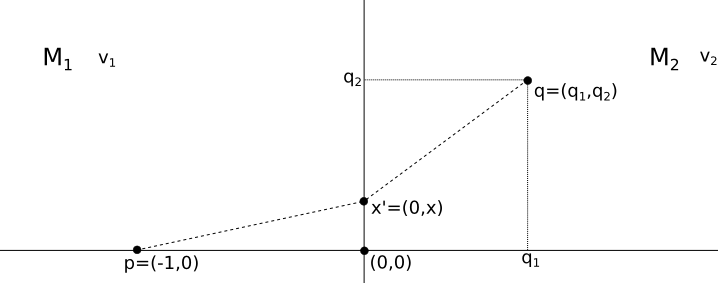
\includegraphics[width=0.60\textwidth]{imgs/esempio-prog-nv.png}}

All'interno dello stesso mezzo, il percorso pi\`u breve tra due punti \`e
ovviamente la retta. Il percorso sar\`a dunque determinato dal parametro
$x$, ordinata del punto in cui il percorso passa da $M_1$ a $M_2$, e
sar\`a composto da due segmenti che uniscono i punti $p=(-1,0),
x'=(0,x), q=(q_1, q_2)$.\\ I due segmenti sono lunghi rispettivamente
$\sqrt{1+x^2}$ e $\sqrt{q_1^2 + (q_2 - x)^2}$.\\ La funzione che
calcola il tempo di percorrenza, da minimizzare, \`e la seguente:
$$f(x) =  \frac{\sqrt{1+x^2}}{v_1} + \frac{\sqrt{q_1^2 + (q_2 - x)^2}}{v_2}$$
Dobbiamo risolvere il problema di ottimizzazione senza vincoli:
$$ \min\{f(x):\; x \in \mathbb{R}\}$$
Cerchiamo i punti in cui il gradiente della funzione si annulla. Dato
che la funzione \`e a una variabile, il gradiente \`e la derivata:
$$\nabla f(x)= f'(x)=0$$

$$f'(x) = \frac{1}{v_1} \frac{2x}{2 \cdot \sqrt{1+x^2}} + \frac{1}{v_2} \frac{2x - 2q_2}{2\sqrt{q_1^2 + (q_2 - x)^2}} = \frac{x}{v_1\sqrt{1+x^2}} - \frac{{q_2 - x}}{v_2 \sqrt{q_1^{2} + (q_2 -x)^2}}
$$
Notiamo che i denominatori non si annullano mai e risolviamo $f'(x) =
0$.
$$ v_2 x \sqrt{q_1^2 + (q_2 -x)^2} - v_1(q_2 -x)\sqrt{1+x^2}=0$$ \\
Abbiamo ottenuto una funzione non lineare che da il punto di
stazionariet\`a. Inoltre la funzione \`e convessa, quindi in questo caso
la condizione $f'(x)=0$ \`e necessaria e sufficiente perch\'e la funziona
sia minima. \\ \textbf{Esercizio}: dimostra che $f'(x)$ \`e convessa.\\
Riscriviamo l'equazione come:

\begin{equation}
\label{eq:esempio-ottimizzazione-nv-1} \frac{x}{\sqrt{1+x^2}} \cdot
\frac{\sqrt{q_1^2 + (q_2-x)^2}}{q_2 -x} =\frac{v_1}{v_2}
\end{equation}

Facciamo intanto un'osservazione. Dato che le velocit\`a sono positive,
\`e
$$\frac{v_1}{v_2} > 0 \quad \Longrightarrow \quad \frac{x}{q_2-x} \geq 0 \quad \Longrightarrow \quad 0 \leq x \leq q_2$$
Abbiamo ristretto lo spazio in cui cercare la soluzione ottimale.

\centerline{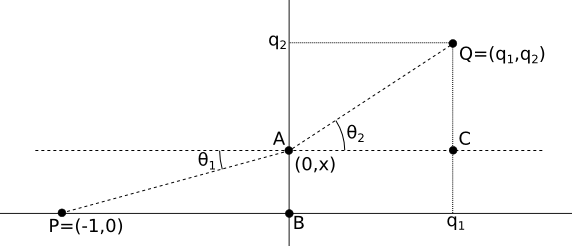
\includegraphics[width=0.50\textwidth]{imgs/esempio-prog-nv2.png}}

Diamo dei nomi ai punti come nella figura sopra e riscriviamo la
\ref{eq:esempio-ottimizzazione-nv-1} rinominando i membri delle
frazioni come:

$$\frac{\overline{AB}}{\overline{PA}} \cdot \frac{\overline{AQ}}{\overline{QC}} = \frac{v_1}{v_2}$$

Guardando la figura, si noti come
$$\frac{\overline{AB}}{\overline{PA}} = \sin \theta_1, \quad \frac{\overline{AQ}}{\overline{QC}} = \frac{1}{\sin \theta_2}$$
Abbiamo ottenuto che la durata di percorrenza $f(x)$ si minimizza
quando
$$ \frac{\sin \theta_1}{\sin \theta_2} = \frac{v_1}{v_2}$$
(Tra l'altro, questa \`e la legge della rifrazione di
Snell--Cartesio.)\\ \`E un'equazione non lineare ad una variabile che si
può risolvere con i classici metodi del calcolo numerico, ad esempio
applicando il Metodo delle Tangenti nell'intervallo $[0, q_2]$.
\end{example}

\begin{example} Nell'esempio \ref{esempio-prog-nv} la funzione che
abbiamo ottenuto per la ricerca del punto stazionario era ad una
variabile. Complichiamo il problema in modo da ottenere una funzione a
due variabili.

\centerline{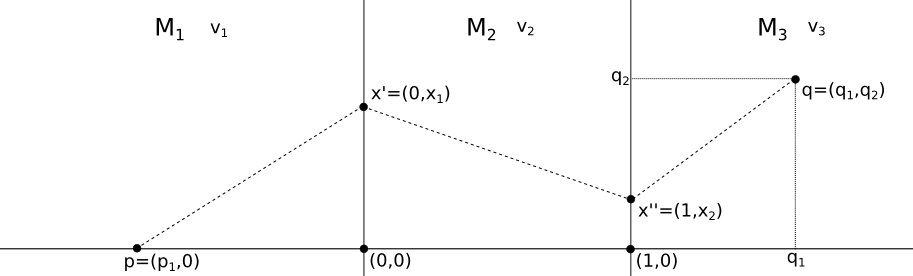
\includegraphics[width=0.80\textwidth]{imgs/esempio-prog-nv-2var.png}}

Il problema \`e simile ma invece di due, i mezzi sono tre: $M_1, M_2,
M_3$, divisi da due rette parallele. Per semplificare i conti,
posizioniamo gli assi in modo che le rette di separazione dei piani
siano verticali e il punto $p$ di partenza sia sull'asse delle
ascisse, e scegliamo un'unit\`a di misura tale che il semipiano $M_2$
sia largo $1$.\\ Stavolta per individuare un tragitto sono necessari i
due parametri $x_1$ e $x_2$, ovvero il valore dell'ordinata dei punti
$x'$ e $x''$ in cui il tragitto passa da un mezzo all'altro.\\ La
funzione che calcola la velocit\`a di percorrenza \`e $$f(x_1, x_2) =
\frac{\sqrt{p_1^2 + x_1^2}}{v_1} + \frac{\sqrt{1+ (x_2 - x_1)^2}}{v_2}
+ \frac{\sqrt{(q_1 -1)^2 + (q_2 - x_2)^2}}{v_3}$$ Abbiamo un problema
di minimizzazione, anche questo non vincolato, in 2 variabili: $$
\min\{f(x):\; x \in \mathbb{R}^2\}$$ $f(x)$ \`e convessa, quindi
$\nabla(x) = 0$ \`e condizione necessaria e sufficiente per la
minimalit\`a di $f(x)$.\\ \textbf{Esercizio}: dimostrare che $f(x)$ \`e
convessa. \\ Cerchiamo dove $$\nabla f(x) = 0$$ Stavolta $\nabla f(x)$
\`e un vettore a due dimensioni. Vediamone le componenti, che si devono
annullare:\\
$$\frac{\partial f}{x_1}(x_1,x_2) =  \frac{x_1}{v_1 \sqrt{p_1^2+ x_1^2}} - \frac{x_2 - x_1}{v_2 \sqrt{1+(x_2 - x_1)^2}} = 0$$
$$\frac{\partial f}{x_2}(x_1,x_2) =  \frac{x_2-x_1}{v_2 \sqrt{1+( x_2-x_1)^2)}} - \frac{q_2 -x_2}{v_3  \sqrt{(q_1-1)^2 + (q_2 -x_2)^2}} = 0$$
Questo \`e un sistema non lineare di due equazioni in due
incognite. Condizione necessaria e sufficiente perch\'e la soluzione
$x=(x_1,x_2)$ sia minima \`e che il sistema sia soddisfatto.

Questo particolare sistema si può risolvere con i metodi classici del
calcolo numerico, ad esempio il metodo delle tangenti (detto anche
Newton--Raphson), cercando sia $x_1$ che $x_2$ nell'intervallo
$[0,q_2]$).
\end{example}

\section{Metodi risolutivi per i problemi di ottimizzazione non
vincolata} Abbiamo visto negli esempi dei problemi che si riducono
alla risoluzione di un sistema non vincolato di equazioni non lineari,
e abbiamo accennato al fatto che questi sistemi, in alcuni casi,
possono essere risolti con i metodi del calcolo numerico (es. Metodo
delle tangenti, delle secanti o di bisezione). Va notato però che
questi metodi hanno bisogno come dato di input dell'intervallo entro
cui cercare la soluzione, e della garanzia che questo intervallo
contenga una sola soluzione. Sebbene questo sia possibile nei due
esempi presi in considerazione, non \`e possibile in generale.

Guardiamo quindi a dei metodi iterativi in grado di risolvere un
generico problema di ottimizzazione non vincolata. Il problema si pone
come
$$ (P) \quad \min\{f(x)\; : \; x \in \mathbb{R}^n\} \quad f: \mathbb{R}^n  \rightarrow \mathbb{R} \text{ differenziabile}$$
I metodi che vedremo sono tutti di natura iterativa, genereranno
dunque una successione di valori $ x^0, x^1, \ldots, x^k$. Quello che
cerchiamo, come sempre, sono i punti stazionari $x^{*}$, ovvero tali
che
$$\nabla f(x^{*}) = 0$$

Se la funzione \`e convessa, come sappiamo $\nabla f(x^{*}) = 0$ \`e
condizione sufficiente, oltre che necessaria, perch\'e $x$ sia punto di
minimo, dunque nelle funzioni convesse i punti stazionari sono anche
punti di minimo. Altrimenti, se $f$ non \`e convessa,$\nabla f(x^{*}) =
0$ \`e comunque condizione necessaria per essere punto di minimo, quindi
siamo comunque interessati a cercare i punti in cui il gradiente si
annulla perch\'e candidati ad essere minimi.

L'unica ipotesi di cui abbiamo bisogno per questo tipo di metodi \`e che
$f$ sia differenziabile (ma in alcuni metodi porremo il vincolo che
$f$ sia differenziabile con continuit\`a, cio\`e che il suo gradiente
$\nabla f$ sia una funzione continua, oppure che sia differenziabile
due volte).

In questi metodi, trovare $\overline{k}$ t.c. $\nabla
f(x^{\overline{k}}) = 0$ può essere un processo infinito. Non potendo
garantire la finitezza, ciò che chiediamo ai nostri metodi \`e la
convergenza, che può essere definita in diversi modi:

\begin{enumerate}
\item Il limite esiste ed \`e un punto stazionario: $$\exists \lim_{k
\to \infty} x^{k} = x^{*} \quad \text{e} \quad \nabla f(x^{*}) = 0$$
\item Definizione pi\`u debole: se la successione converge, allora
converge al punto stazionario (ma non \`e detto che converga!). Quindi
tutti i punti di accumulazione di $\{x^k\}$ sono stazionari (ma non \`e
detto che ne esistano): $$\lim_{k \to \infty} x^{k} = x^{*} \quad
\Longrightarrow \quad \nabla f(x^{*}) = 0$$
\item Definizione ancora pi\`u debole: almeno un punto di accumulazione
della successione $\{x^k\}$ \`e stazionario.
\end{enumerate}

Tra i metodi iterativi, daremo particolare attenzione ai Metodi di
discesa:
\begin{defn}[Metodo di discesa] Quei metodi iterativi tali che ad ogni
iterazione, il valore della funzione obiettivo decresce: $$ f(x^0) >
f(x^1) > f(x^2) > \ldots > f(x^k) > \ldots $$
\end{defn}

In particolare, si dice Metodo di discesa \emph{non
monotòna}\footnote{Utilizzeremo raramente questa definizione.} se:
\begin{defn}[Metodo di discesa non monotòna] Dopo $n$ iterazioni ($n$
fissato), il valore della funzione obiettivo decresce:
$$ \exists ~ n \in \mathbb{N} \quad \text{t.c.} \quad \forall k \quad f(x^k) > f(x^{k+n}) $$
\end{defn}

\subsection{Ricerca monodimensionale} Nei metodi di ricerca
monodimensionale (line search), se nella $k$-esima iterazione abbiamo
ottenuto il punto $x^k$, otteniamo il punto $x^{k+1}$ muovendoci dal
punto $x^k$ lungo una direzione $d^k$ di un passo lungo $t_k$
(direzione e ampiezza del passo sono scelti ad ogni iterazione). Si
chiama \emph{monodimensionale} proprio perch\'e l'ampiezza del passo
$t_k$ \`e scelta su un'unica dimensione (lungo $d^k$). Tipicamente si
sceglie $d^k$ t.c. $\Vert d^k \Vert = 1$.

\centerline{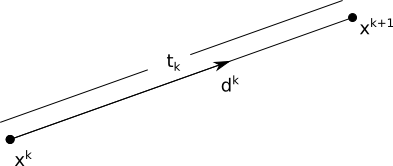
\includegraphics[width=0.40\textwidth]{imgs/ricerca-monodimensionale-passo.png}}

In formule:
$$ x^{k+1} = x^{k} + t_k d^{k} \quad t_k \in \mathbb{R}^{n} \quad
  \begin{array}{l} t_k \in \mathbb{R}\text{ passo di spostamento} \\
d^{k} \in \mathbb{R}^n \text{ direzione}
  \end{array}
$$
%$$ t_k \in argmin \{ f(x^{k}+td^{k}) : t \geq 0  \}$$

\begin{notes} Anche l'algoritmo del simplesso per la programmazione
lineare vincolata \`e un metodo di line search, visto che da un vertice
ci si muove lungo una direzione (cio\`e lungo il bordo dei vincoli) per
giungere ad un altro vertice.
\end{notes}

I metodi di ricerca monodimensionale si differenziano tra loro
per il modo in cui, ad ogni passo, viene scelta la
direzione $d$ e l'ampiezza $t$ del passo successivo.

Vediamo innanzi tutto come ottenere un metodo di discesa. Supponiamo,
ad un generico passo, di aver ottenuto $ \overline{x} \in
\mathbb{R}^{n}$ (non stazionario, cio\`e tale che $\nabla
f(\overline{x}) \neq 0$, altrimenti abbiamo gi\`a la soluzione).

Dato che $f$ \`e differenziabile, abbiamo lo sviluppo di Taylor:
$$f(\overline{x} +t \cdot d) -f(\overline{x}) = t \cdot \nabla f(\overline{x})^{T} \cdot d + r(td)$$

Dove $r(td)$ \`e un resto tale che $\frac{r(td)}{t}$ va a $0$ per $||t|| \longrightarrow 0$. Inoltre
sappiamo che

$$ \lim_{t \to 0} \frac{f(\overline{x}+td)- f(\overline{x})}{t} = \nabla f(\overline{x})^{T} \cdot d $$

Da questa equazione si ricava che, se scegliamo la direzione $d$ in
modo che sia $\nabla f(\overline{x})^{T} \cdot d < 0$, in un intorno
di $t=0$ sufficientemente piccolo l'argomento del limite deve essere
negativo:

$$\exists ~ \varepsilon ~ \text{t.c.}~ \forall ~ t \in [0,\varepsilon] \quad \frac{f(\overline{x}+td)- f(\overline{x})}{t} < 0$$

ma dato che $t>0$, deve necessariamente essere $f(\overline{x}+td)-
f(\overline{x}) < 0$ e dunque $f(\overline{x}+td) < f(\overline{x})$,
che \`e proprio ciò che cercavamo.

Ricapitolando:
\begin{property}
\label{prop:metodo-discesa-gradiente-direzione} se si sceglie
$$d \quad \text{t.c.} \quad \nabla f(\overline{x})^{T} \cdot d < 0 \quad \text{e} \quad  t \in (0, \varepsilon) \text{ con }\varepsilon\text{ sufficientemente piccolo} \quad \Longrightarrow \quad \text{il passo } x^{k} + t_k d^{k} \text{ \`e di discesa} $$
\end{property}
\subsection{La massima decrescita}
\label{subsection:massima-decrescita} Naturalmente, il nostro
interesse \`e che il metodo non solo sia di discesa, ma che discenda pi\`u
velocemente possibile. Cerchiamo quindi di prendere $d$ in modo che il
prodotto non solo sia negativo, ma il pi\`u negativo possibile. Per
andare incontro a questa esigenza, si forma un altro problema:
\begin{equation}
\label{prob:pa} (Pa) \quad \min \{ \nabla f(\overline{x})^{T}d :
||d||_2 = 1 \}
\end{equation}

\begin{notes} La norma di $d$ deve essere limitata, ad es. con
$||d||_2 = 1$, altrimenti supponiamo di trovare una direzione
$$ \overline{d} = dt \quad \text{t.c.} \quad \nabla f(\overline{x})^{T} \overline{d} < 0 \quad \Longrightarrow \quad\nabla f(\overline{x})^{T} \overline{d} = \nabla f(\overline{x})(td) = t(\nabla f(\overline{x})^{T}d)$$
Ma se mandiamo $t$ a $+\infty$:
$$t(\nabla f(\overline{x})^{T}d) \longrightarrow_{t \to +\infty} - \infty$$
E il problema risulta inferiormente illimitato.
\end{notes}

Il problema di ottimizzazione \ref{prob:pa} lo sappiamo risolvere per
via teorica. Si ricorda che il prodotto scalare tra due vettori $a$ e
$b$ si calcola come

\centerline{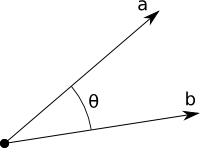
\includegraphics[width=0.20\textwidth]{imgs/a-b-theta.png}}

$$a^{T}b = ||a||_{2} ||b||_2 \cos \theta$$
Quindi tenendo conto che $||d||_2 = 1$, il prodotto scalare
$f(\overline{x})^{T}d$ si calcola come
$$\nabla f(\overline{x})^{T} d =  || \nabla f(\overline{x})||_{2} \cos \theta$$
In cui $\overline{x}$ e $f$ sono fissati, quindi $f(\overline{x})$ \`e
un numero fissato nel nostro problema.

Quindi il problema si può riscrivere come:
$$ \min \{ \nabla f(\overline{x})^{T}d ~ : \Vert d \Vert = 1 \} ~ =  ~ \Vert\nabla f(\overline{x})\Vert_{2} \cdot \min\{ \cos \theta ~ : \Vert d \Vert_{2}=1 \}$$
Notare che $d$ sembra scomparire nella formula, in realt\`a $\theta$
dipende da $d$ (e da $f(\overline{x})$ che \`e fisso per il problema).
Il minimo di questo problema si ottiene quando
$$ \cos \theta = -1 \quad \Longleftrightarrow \quad  \theta = \pi $$

Ma perch\'e questo angolo sia $\pi$, \`e necessario che si prenda $d$
nella direzione opposta rispetto al gradiente. Inoltre vogliamo $d$ di
norma unitaria, e per questo basta dividerlo per la norma del
gradiente.
$$\quad \Longleftrightarrow \quad d = \frac{- \nabla f(\overline{x})}{|| \nabla f(\overline{x})||_{2}}$$
In altre parole, sto chiedendo che $d$ sia il versore della direzione
opposta al gradiente.

Ancora una volta, il gradiente \`e la direzione di massima crescita,
quindi la massima decrescita \`e la direzione opposta al gradiente.

\section{Metodi del gradiente} Da quanto visto sopra, si deduce
facilmente un primo metodo di ricerca monodimensionale in cui la
direzione $d$ scelta ad ogni passo \`e l'opposto del gradiente:

$$ x^{k+1} = x^{k} + t_k \cdot d^k \quad \text{con} ~ d^{k} = - \nabla f(x^{k})$$
Ovvero
$$ x^{k+1} = x^{k} - t_k \cdot \nabla f(x^{k})$$

(Avremmo potuto prendere $d^k = - \frac{\nabla f(k^k)}{\Vert \nabla
f(x^k)\Vert_{2}}$, ma lasciamo perdere la divisione per la norma del
gradiente perch\'e la consideriamo ``inglobata'' nel passo di
spostamento.)

Per quanto riguarda la scelta del passo di spostamento $t_k$, la
scelta ideale \`e ovviamente di prenderlo esatto:
\begin{defn}[Metodo della Ricerca Esatta] Metodo nel quale la
lunghezza del passo si calcola con un nuovo problema di
ottimizzazione:
$$ t_k \in \text{ arg min } \{f(x^{k} - t_k \nabla f(x^{k})): \; t_k \geq 0 \}$$
Ovvero il passo \`e cercato lungo la semiretta in modo che minimizzi la
funzione obiettivo.
\end{defn}

\begin{defn}[Metodo del Gradiente Esatto]
\label{def:metodo-gradiente-esatto} Metodo del gradiente (ovvero tale
che $d^{k} = - \nabla f(x^{k})$) in cui si sceglie il passo col metodo
della ricerca esatta.

Sotto forma di algoritmo si può enunciare come segue:
\begin{enumerate}
 \item Poniamo $k=0$; Si sceglie un punto di partenza $x_0$;
 \item Se $\nabla f(x^{k})=0$, allora STOP: abbiamo trovato un punto
stazionario. \label{passo-algoritmo-gradiente-esatto-test-stop}
 % un label e' per sempre!
\item Si calcola la direzione come l'opposto del gradiente: $ d^k = - \nabla
 f(x^{k})$;\label{passo-algoritmo-gradiente-esatto-scelta-direzione}
 \item \label{passo-algoritmo-gradiente-esatto-scelta-passo}Si calcola
il passo con la ricerca esatta:
$$t_k \in argmin \{ f(x^{k} + t_k
\cdot d^k) \; : \; t_k \geq 0 \}$$
ovvero
$$t_k \in argmin \{ f(x^{k} - t_k
\cdot \nabla f(x^{k})) \; : \; t_k \geq 0 \}$$
 \item Ci si sposta al punto successivo: $x^{k+1} =x^{k} + t_k \cdot d^k = x^{k} - t_k \cdot
\nabla f(x^{k})$
 \item $k:=k+1$, ritornare al passo
\ref{passo-algoritmo-gradiente-esatto-test-stop}.
\end{enumerate}
\end{defn}

Come vedremo in seguito (\ref{critica-gradiente-esatto}), il passo
\ref{passo-algoritmo-gradiente-esatto-scelta-passo} impone la
soluzione di un problema di ottimizzazione esatta che, in generale, \`e
tutt'altro che banale, per questo vedremo altri metodi del gradiente
che non utilizzano la ricerca esatta ma scelgono il passo in maniera
pi\`u approssimata e meno costosa. Tuttavia per alcune funzioni
obiettivo particolari, ad es. le funzioni quadratiche, il calcolo
della ricerca esatta \`e possibile e facilmente risolvibile, perch\'e la
funzione da minimizzare $f(x^{k} - t_k \nabla f(x^{k}))$ \`e una
parabola con il vertice verso l'alto, della quale \`e facile calcolare
esattamente il minimo.

\subsection{Propriet\`a del Metodo del Gradiente Esatto} Abbiamo
intenzione di dimostrare tre propriet\`a del Metodo del Gradiente
Esatto:
\begin{enumerate}
\item Il metodo del gradiente esatto \`e un metodo di discesa;
\item Due direzioni successive del metodo del gradiente esatto sono
tra loro ortogonali;
\item Il metodo converge.
\end{enumerate}

Per queste dimostrazioni, si introduce la seguente funzione:
$$\varphi(t) = f(x^{k} - t \nabla f(x^{k}))$$
Questa \`e la funzione $f$ calcolata lungo la semiretta nella quale
viene cercato il passo di spostamento, vista come funzione del passo
$t$. \`E la funzione di ricerca: durante la ricerca esatta si cerca il
minimo di $\varphi$. Si noti che \`e la composizione di due funzioni:
$$ t \xlongrightarrow{\theta} x^{k}-t\nabla f(x^{k}) \xlongrightarrow{f} f(x^{k} - t \nabla f(x^{k}))$$

La funzione $\theta: \mathbb{R} \rightarrow \mathbb{R}^{n}$ associa il
passo $t$ al punto trovato, mentre $f: \mathbb{R}^{n} \rightarrow
\mathbb{R}$ associa il punto trovato al valore della funzione
obiettivo. $\varphi$ si scrive come $ \varphi= f \circ \theta :
\mathbb{R} \rightarrow \mathbb{R}$.

$\theta$ si può vedere come un insieme $(\theta_{1}, \ldots,
\theta_{i}, \ldots, \theta_{n})$ di $n$ funzioni, una per ogni
componente, tali che $\theta_{i}: \mathbb{R} \rightarrow \mathbb{R}$
assume il valore dell'$i$-esima componente del vettore $x^{k}-t\nabla
f(x^{k}) = \theta(t)$. Quindi

$$ \theta = (\theta_{1}, \theta_{2}, \ldots, \theta_{n}) \qquad \theta(t) = x^{k}-t\nabla f(x^{k}) =  \left(\begin{matrix}\theta_{1}(t) \\\theta_{2}(t) \\ \vdots \\ \theta_{n}(t)\end{matrix}\right)$$

La funzione $\theta$ \`e derivabile, quindi ogni $\theta_i$ \`e
derivabile.
$$ \theta' = (\theta_1', \theta_2', \ldots, \theta_{n}' )$$

Si noti quindi che
$$
\left.\begin{matrix} f \text{ \`e differenziabile}\\ \theta_i \text{
sono derivabili} \\
\end{matrix}\right. ~ \Longrightarrow ~ \varphi = f \circ \theta
\text{ \`e derivabile}
$$

e la sua derivata \`e \footnote{ Usando il seguente teorema
  \begin{theo}
    \label{theo:derivata-funzioni-composte} Sia $\Theta:\mathbb{R}
\rightarrow \mathbb{R}^{n}$ derivabile in $\overline{t}\in \mathbb{R},
g: \mathbb{R}^{n}$ differienziabile in $\Theta(\overline{t})\in
\mathbb{R}^{n}$. \\ Allora $ g \circ \Theta$ \`e differenziabile in
$\overline{t}$ e $(g \circ \theta)'(\overline{t}) = \nabla
g(\Theta(\overline{t}))^{T} \Theta'(\overline{t})$.  (dove $\Theta' =
(\Theta'_1, \ldots , \Theta'_n), \; \Theta = (\Theta_1, \ldots
\Theta_n)$
  \end{theo}}:

$$ \varphi'(t) = \nabla f(x^{k} - t \nabla f(x^k))^T \cdot \theta'(t)$$

Ma dato che $ \theta'(t) = - \nabla f(x^k)$,

\begin{equation}
\label{eq:derivata-phi} \varphi'(t) = -\nabla f(x^{k} - t \nabla
f(x^{k}))^{T} \cdot \nabla f(x^{k})
\end{equation}

Questo strumento ci permetter\`a di fare facilmente tutte e tre le
dimostrazioni.

Sappiamo inoltre che:
\begin{enumerate}
\item Nel punto di minimo, che \`e $t_k$, la derivata si annulla: $$
\varphi'(t_k) = 0$$
\item Il valore che questa derivata assume nel punto $0$ (si calcola
esplicitamente): $$\varphi'(0) = -||\nabla f(x^{k})||_{2}^{2} < 0$$ \`E
$<0$ perch\'e \`e una norma diversa da $0$ (se il punto non \`e stazionario)
con un meno davanti.
\end{enumerate}

Possiamo sfruttare il risultato in \ref{eq:derivata-phi} e i due sopra
per dimostrazione le tre propriet\`a enunciate sopra.

\begin{theo} Il metodo del gradiente esatto \`e di discesa, ovvero
$\forall k \quad f(x^{k+1}) < f(x^{k})$
\begin{thproof}
$$f(x^{k}) = \varphi(0) \geq \underbrace{\varphi(t_{k})}_{\text{punto di minimo}} = f(x^{k+1})$$
Abbiamo dimostrato $f(x^{k+1}) \leq f(x^{k})$, ma \`e possibile che
siano uguali?

Guardiamo cosa succede nell'intorno di $0$. Se $\varphi'(0) < 0$, la
funzione $\varphi$ e' decrescente almeno nell'intorno, ne segue che
$0$ non può essere un punto di minimo, quindi
$$f(x^{k}) = \varphi(0) \neq \varphi(t_{k}) = f(x^{k+1})$$

Da cui
 $$f(x^{k}) = \varphi(0) > \varphi(t_{k}) = f(x^{k+1})$$
\end{thproof}
\end{theo}

\begin{theo}
\label{theo:gradiente-esatto-direzioni-ortogonali} Due direzioni
successive del metodo del gradiente esatto sono tra loro ortogonali,
ovvero $$ \nabla f(x^{k+1})^{T} \cdot \nabla f(x^{k}) = 0$$
\centerline{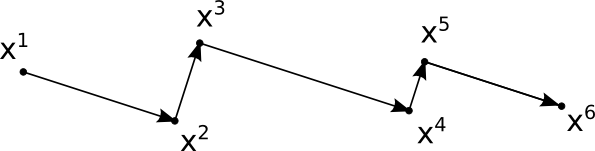
\includegraphics[width=0.40\textwidth]{imgs/direzioni-ortogonali.png}}

\begin{thproof} Sappiamo che $$ \varphi'(t_{k}) = 0 \qquad x^{k+1} =
x^{k} - t_k \nabla f(x^{k})$$ Ma sappiamo anche da
\ref{eq:derivata-phi} che la derivata vale
$$\varphi'(t_{k}) = - \nabla f(x^{k+1})^{T} \nabla f(x^{k}) = 0$$
\end{thproof}
\end{theo}

\begin{theo} Il metodo converge (se esiste il limite, allora il limite
\`e un punto stazionario):
$$\lim_{k \to \infty} f(x^k) = x^* \in \mathbb{R}^n \quad \Longrightarrow \quad \nabla f(x^*) = 0 $$
\begin{thproof} Dal \ref{theo:gradiente-esatto-direzioni-ortogonali}
sappiamo che
$$ \nabla f(x^{k+1})^{T} \nabla f(x^{k})= 0$$

Inoltre
$$\text{per } k \to \infty, \quad x^k \to x^*\text{ e }x^{k+1} \to x^*$$

Per ipotesi, la funzione \`e differenziabile con continuit\`a (cio\`e la
funzione gradiente \`e continua), quindi per la continuit\`a delle
funzioni

$$ \nabla f(x^{k+1})^{T} \nabla f(x^{k}) \longrightarrow_{k \to +\infty} 
    \nabla f(x^{*})^{T} \nabla f(x^{*}) = \Vert \nabla
f(x^{*})\Vert_{2}^{2}$$
      
Quindi $$\Vert \nabla f(x^{*})\Vert_{2}^{2} = 0 \quad \Longrightarrow
\quad \nabla f(x^*) = 0$$
$$\nabla f(x^*) \text{ \`e stazionario.}$$
\end{thproof}
\end{theo}

\subsection{Critica al metodo del gradiente esatto}
\label{critica-gradiente-esatto}
\paragraph{Critica al Passo
\ref{passo-algoritmo-gradiente-esatto-scelta-passo} (e caso
particolare delle funzioni quadratiche)} Come accennato, il passo
\ref{passo-algoritmo-gradiente-esatto-scelta-passo} del Metodo del
Gradiente Esatto (vedi la sua definizione
\ref{def:metodo-gradiente-esatto}), nel quale viene calcolata
l'ampiezza del passo di spostamento, \`e un problema pi\`u semplice
rispetto a cercare il minimo di una funzione, ma in generale \`e
comunque costoso. Il calcolo del minimo di $\varphi(t)$ \`e un problema
ad una sola variabile (invece di $n$), ovvero \`e un problema di
ottimizzazione monodimensionale, ma richiede comunque una procedura
algoritmica.

Vi sono tuttavia dei casi in cui il calcolo esatto del passo di
spostamento non richiede un algoritmo: nel caso in cui $f$ sia una
funzione quadratica, come vedremo ci non troviamo pi\`u davanti ad un
problema di ottimizzazione ma semplicemente al calcolo di una formula.

Si ricorda la definizione di funzione quadratica:
$$f(x) = \frac{1}{2} x^{T} Qx + b^{T}x + c \quad Q = Q^{T} \in \mathbb{R}^{n\times n} ,b \in \mathbb{R}^{n}, c \in \mathbb{R}$$

Dove $Q$ \`e una matrice quadrata e che, aggiustando i coefficienti,
possiamo rendere anche simmetrica. Avevamo visto che il gradiente di
questa funzione \`e
$$ \nabla f(x) = Qx +b $$

Per cui trovare i punti stazionari equivale a trovare soluzioni del
sistema lineare

$$ \nabla f(x) = Qx +b = 0$$

\begin{property} Il problema ha senso se $Q$ \`e semi-definita
positiva. Vediamo cosa succederebbe in caso contrario: se non fosse
semi-definita positiva, allora vi sarebbe un $\overline{x} \in
\mathbb{R}^n$ tale che $\overline{x}^T Q \overline{x} < 0$. Inoltre
$f$ in $t\overline{x}$ varrebbe
$$f(t \overline{x}) = \frac{1}{2} t^2 (\overline{x}^T Q \overline{x}) + t b^T \overline{x} + c$$

Questa, come funzione di $t$, \`e una parabola con il coefficiente del
termine quadrato ($\overline{x}^T Q \overline{x}$) negativo. Dunque il
suo limite per $t \to \infty$ \`e
$$\lim_{t \to +\infty} f(t \overline{x}) = - \infty$$

Abbiamo trovato che se esiste un punto $\overline{x}$ che vìola il
fatto che $Q$ sia semi-definita positiva, si ottiene che in quella
direzione la funzione obiettivo va a $-\infty$, il problema risulta
dunque inferiormente illimitato. Non ha dunque senso la minimizzazione
vincolata di una funzione quadrata che non sia semi-definita positiva.
\end{property}

Si ricorda che $\varphi$ \`e definita come \footnote{Rispetto alla
definizione precedente abbiamo rinominato $x^k$ in $x$ per
semplicit\`a.}
$$\varphi(t) = f(x -t \nabla f(x))$$

Dato che $Q$ \`e semi-definita positiva, possiamo calcolare la
derivata di $\varphi(t)$
$$
\begin{array}{rl} \varphi'(t) &= -\nabla f(x -t \nabla f(x))^{T}
\nabla f(x) \\ &= -[Q(x -t \nabla f(x)) + b]^{T} \cdot \nabla f(x) \\
&= -[Qx -t Q \nabla f(x) + b]^{T} \cdot \nabla f(x) \\ &= -[\nabla
f(x) -t Q \nabla f(x)]^{T} \cdot \nabla f(x) \\ &= -\nabla f(x)^{T}
\cdot \nabla f(x) + t \underbracket{\nabla f(x)^{T} Q \nabla
f(x)}_{\geq 0}
\end{array}
$$

Cerchiamo di vedere dove si annulla la derivata $\varphi'$. Abbiamo
che $\nabla f(x)^{T} Q \nabla f(x) \geq 0 $ perch\'e $Q$ \`e semi-definita
positiva. Distinguiamo due casi:
\begin{enumerate}
\item Se $\nabla f(x)^{T} Q \nabla f(x) >0$ (questo \`e sempre vero se
$Q$ \`e definita positiva) allora il gradiente si annulla nel punto
$$ t= \frac{\nabla f(x)^{T} \nabla f(x)}{\nabla f(x)^{T}Q \nabla f(x)} \quad \Longleftrightarrow \quad \varphi'(x) = 0$$
\item Altrimenti, se $\nabla f(x)^{T} Q \nabla f(x) =0$ (possibile
solo se $Q$ \`e semi-definita positiva) allora
$$ \varphi'(t) = -\nabla f(x)^{T} \nabla f(x)  = \underbrace{-\Vert \nabla f(x)\Vert_{2}^{2}}_{<0}$$
che \`e costante e $\neq 0$. Ma se $\varphi$ ha derivata costante e
negativa, significa che \`e una funzione lineare (una retta) nella forma
$$\varphi(t) = f(x-t \nabla f(x)) = - \Vert \nabla f(x)\Vert_{2}^{2} t + costante$$
E il suo limite
$$ \lim_{t \to +\infty}{\varphi(t)}  = - \infty$$
Quindi, se con una certa matrice $Q$ si incontra la condizione $\nabla
f(x)^{T} Q \nabla f(x) =0$ (può succedere solo se $Q$ \`e semidefinita
positiva, non se \`e definita positiva) allora il problema \`e
inferiormente illimitato.
\end{enumerate}

Ricapitolando, il caso che la funzione obiettivo $f$ sia quadratica
non pone problemi con la ricerca esatta:
\begin{itemize}
\item Se $Q$ non \`e semidefinita positiva, il problema \`e inferiormente
illimitato.
\item Altrimenti abbiamo la formula esplicita per calcolare il passo
di spostamento: $t= \frac{\nabla f(x)^{T} \nabla f(x)}{\nabla f(x)^{T}Q \nabla f(x)}$
\item Se si pone la condizione $\nabla f(x)^{T} Q \nabla f(x) =0$
(impossibile se $Q$ \`e definita positiva) allora il problema \`e
inferiormente illimitato.
\item Se $f$ non \`e quadratica, per trovare il minimo di $\varphi$,
ovvero la lunghezza del passo di spostamento, ha bisogno di metodi
iterativi (es. tangenti, secanti, newton) e dunque inesatti.
\end{itemize}

\paragraph{Funzione ripida} Può succedere che nei pressi di un punto
stazionario, le curve di livello siano estremamente ripide. \`E questo
il caso della Funzione di Rosenbrock, definita come:
\begin{equation}
\label{eq:rosenbrok-banana} f(x,y) = (1-x)^2 + 100(y-x^2)^2
\end{equation}

\begin{figure}[h!]   \centering
    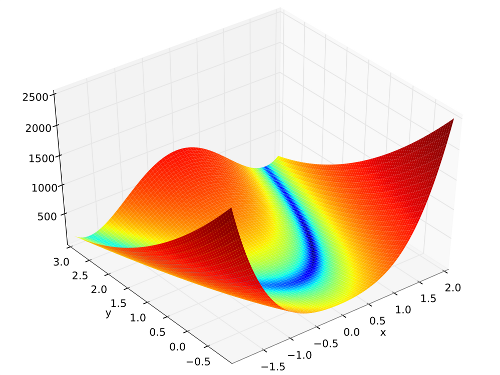
\includegraphics[width=0.60\textwidth]{imgs/rosenbrock-banana.png}
  \caption{Funzione banana di Rosenbrock in tre dimensioni. Immagine
presa da Wikipedia,
\url{http://en.wikipedia.org/wiki/Rosenbrock_function}.}\label{img:rosenbrock-banana}
\end{figure}


Si vede ad occhio che in $(1,1)$ la funzione vale $f(1,1) = 0$ ed
essendo $f$ la somma di due quadrati, non può esservi un punto
minore. Tuttavia questa funzione ha la capacit\`a di rompere tutti i
metodi iterativi per la ricerca del minimo locale, perch\'e la discesa
verso questo minimo \`e molto ripida. Il metodo del gradiente esatto,
una volta entrato nel ``canale'' (la parte blu nella Figura \ref{img:rosenbrock-banana}), essendo
un metodo di decrescita ed avendo le direzioni tra passi successivi
ortogonali tra loro \`e costretto a fare passi molto brevi per non
risalire sull'altra sponda del canale, e quindi \`e estremamente lento.

\paragraph{Critica al passo
\ref{passo-algoritmo-gradiente-esatto-scelta-direzione} (Direzioni
ortogonali)} Abbiamo visto nel Teorema
\ref{theo:gradiente-esatto-direzioni-ortogonali} che la direzione del
passo all'iterazione $k$ \`e ortogonale a quella del passo $k+1$. Gli
spostamenti sono quindi rigidi. Se siamo lontani dal punto stazionario
il fatto di avere direzioni ortogonali non crea problemi, ma quando ci
si avvicina può portare a dei passi molto piccoli e quindi un
rallentamento della convergenza.

Si ricorda che la direzione di spostamento, scelta al passo
\ref{passo-algoritmo-gradiente-esatto-scelta-direzione} dell'algoritmo
in \ref{def:metodo-gradiente-esatto}, \`e ortogonale rispetto a quella
del passo precedente perch\'e \`e scelta come il gradiente. Vediamo dei
modi alternativi per scegliere la direzione, sempre in modo che il
metodo sia di decrescita.

\paragraph{Direzioni alternative di decrescita}
\label{par:direzioni-alternative-decrescita} Possiamo scegliere $d^{k}
= -D_{k} \nabla f(x^{k})$ con $D_k \in \mathbb{R}^{n\times n}$
definita positiva, ovvero data la direzione del gradiente, la
alteriamo moltiplicandola per una matrice scelta ad ogni passo.

Si noti che questa \`e la generalizzazione della scelta del gradiente
usata finora, infatti per ottenere $d^{k} = -\nabla f(x^{k})$,
basta scegliere $D_k = I$.

Se $D_k$ \`e definita positiva, secondo la propriet\`a
\ref{prop:metodo-discesa-gradiente-direzione}, almeno vicino al punto
$x^k$, la direzione $d^k$ \`e di discesa perch\'e
    $$ \nabla f(x^{k})^{T} d^{k} = - \nabla f(x^{k})^{T} D_k \nabla f(x^{k})< 0$$

Tuttavia, sebbene finora ci siamo accontentati di decrescere, questa
propriet\`a in generale non basta. Ad esempio, un metodo di decrescita
applicato su una parabola potrebbe generare la sequenza di punti in
figura:

\centerline{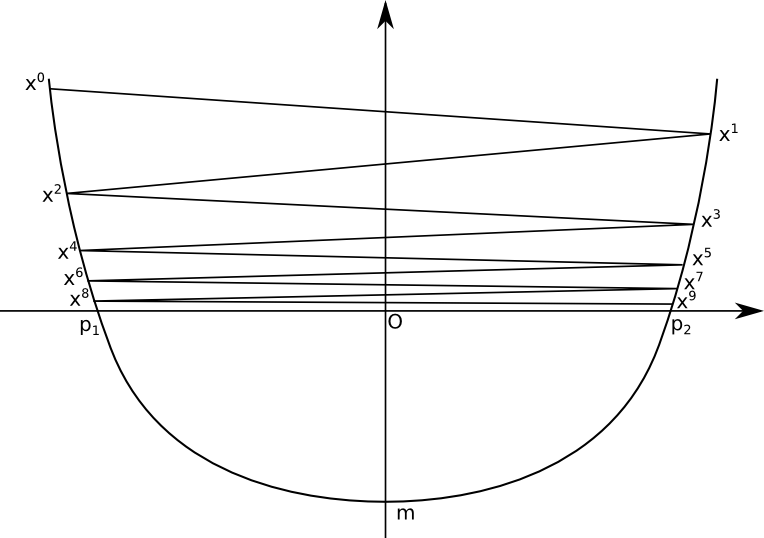
\includegraphics[width=0.60\textwidth]{imgs/parabola-no-convergenza.png}}

Come si vede, il valore della funzione obiettivo decresce ad ogni
iterazione, ma le due sottosuccessioni convergono ai due punti $p_1$ e
$p_2$, che non hanno niente a che fare con il minimo $m$, molto
distante.

Quindi la ricerca esatta può essere una richiesta eccessiva, ma
comunque dobbiamo porre dei paletti pi\`u rigidi della semplice
decrescita. Esistono diverse propriet\`a, di diversa rigidit\`a, che i
metodi possono offrire:
\paragraph{Possibili scelte per il passo}
\begin{itemize}
\item Ricerca esatta: $$ t_k \in argmin \{ f (x^{k} + td^{k}) : t \geq
0 \}$$ Ovvero lungo la direzione $d^k$ (che in generale non \`e $\nabla
f(x^k)$) si prende il minimo. Abbiamo visto che in generale
individuare il minimo in maniera esatta \`e difficile o impossibile.
\item Minimizzazione limitata: $$ t_k \in argmin \{ f (x^{k} + td^{k})
: t \in [0,T]\} \quad T \geq 0 $$ $T$ \`e un valore fissato scelto
dall'utente. Serve per limitare la ricerca a passi non troppo grandi,
che potrebbero mandare troppo fuori strada.
\item Costante: $$t_k = \overline{t}, \quad \overline{t}> 0$$ Il passo
\`e sempre ampio $\overline{t}$ definito dall'utente. Il rischio \`e che
se $\overline{t}$ \`e troppo grande, quando si \`e vicini al punto
stazionario si cominci a girarci intorno, se invece \`e troppo piccolo
l'avvicinamento nelle iterazioni iniziali sia lento.
\item Passi decrescenti: $$ t_{k} \downarrow 0 \quad\text{ con }
\sum_{k=0}^{\infty} t_k = + \infty$$ Ovvero i passi sono decrescenti
ma la serie dei passi deve divergere, ad esempio si può scegliere
$t_{k} = \frac{1}{k}$ ma non $t_{k} = \frac{1}{k^2}$ che converge a
$0$.
\item Ricerca inesatta: \`e come la ricerca esatta, ma invece del minimo
cerchiamo una sua approssimazione, ponendo delle condizioni sulla
decrescita, in modo che il processo sia meno oneroso.
\end{itemize}

\subsection{Metodi del gradiente con ricerca inesatta} Vediamo quali
sono i paletti che dobbiamo porre per la ricerca inesatta, e come
potrebbe funzionare un metodo basato sulla ricerca inesatta. La
situazione che abbiamo davanti \`e la stessa del Metodo del gradiente
esatto (\ref{def:metodo-gradiente-esatto}): da un punto $x^k$ abbiamo
individuato (passo
\ref{passo-algoritmo-gradiente-esatto-scelta-direzione}) una direzione
di discesa $d^k$. Vogliamo però sostituire il passo
\ref{passo-algoritmo-gradiente-esatto-scelta-passo}, ovvero la scelta
del passo $t_k$.

Abbiamo detto che non si cerca il minimo, però vogliamo che la
decrescita sia consistente. Cerchiamo quindi un $t_k$ in modo che sia
rispettata la
\begin{defn}[Condizione di Armijo]
\label{def:condizione-armijo}
$$  \text{(AJO)} \qquad  f(x^{k}+ td^{k}) \leq  f(x^{k}) + c_1 t \nabla f(x^{k})^{T} d^{k}$$
con $ c_1\in (0,1)$ un parametro fissato.

La funzione nel nuovo punto non solo \`e minore della funzione nel
vecchio punto, ma \`e anche pi\`u piccola di almeno $c_1 t \nabla
f(x^{k})^{T} d^{k}$, dove $c_1$ \`e il grado di libert\`a lasciato
all'algoritmo.
\end{defn}

\begin{property}
\label{prop:armijo-tk-non-infinito} Supponiamo la funzione da
minimizzare sia inferiormente limitata (altrimenti il metodo non
serve) e rispetti la condizione di Armijo, allora questo impedisce che
$ t_k \rightarrow + \infty$.

\begin{thproof} Se andasse $ t_k \rightarrow + \infty$,
allora $$\lim_{k \to \infty} (f(x^{k}) + c_1 t_k \underbrace{\nabla
f(x^{k})^{T}d^{k}}_{<0} ) = -\infty$$ ma dato che

$$f(x^{k} + td^{k}) \leq f(x^{k}) + c_1 t_k \nabla f(x^{k})^{T}d^{k} \quad \Longrightarrow \quad f(x^{k} + td^{k}) \rightarrow -\infty$$
che \`e impossibile perché abbiamo assunto che $f$ sia inferiormente
limitata.
\end{thproof}
\end{property}

Quindi la condizione di Armijo impedisce che il passo sia troppo
grande. Ma non impedisce che il passo sia troppo piccolo! Vediamo per
quale motivo.

\begin{property}
\label{prop:condizione-armijo-sempre-valida-in-intervallo} Esiste
sempre un intervallo, per quanto piccolo, in cui la condizione di
Armijo \`e rispettata.
\begin{thproof} Abbiamo visto che
$$\varphi'(0) = \nabla f(x^{k})^{T} d^{k} < 0 $$
Inoltre,
$$ \varphi'(0) = \lim_{t \to 0} \frac{f(x^{k} + td^{k}) - f(x^{k})}{t}$$
e dalla definizione di limite, si può dire che
$$ \exists  ~ \overline{t} \text{ t.c. (AJO) vale } \forall t \in [ 0, \overline{t}]$$

Essendo $\nabla f (x^k)^T d^k < 0$ e $c_1 \in (0,1)$, risulta $\nabla
f (x^k)^T d^k < c_1 \nabla f (x^k)^T d^k$

Quindi per un $t$ sufficientemente piccolo, vale
$$ \frac{f(x^{k} + td^{k}) - f(x^{k})}{t} < c_1 \nabla f (x^k)^T d^k $$
Ma riscrivendola:
$$ f(x^{k} + td^{k}) < f(x^{k}) + t \cdot c_1 \nabla f (x^k)^T d^k $$
abbiamo ottenuto proprio la condizione di Armijo.
\end{thproof}
\end{property} Cosa significa questo? Che sebbene la condizione di
Armijo impedisca passi troppo grandi, \`e soddisfatta da un
\underline{qualunque} valore del passo che sia sufficientemente
piccolo.

Quindi la condizione non basta. Dobbiamo imporre qualche altra
condizione per cui il passo non sia troppo piccolo. Ad esempio, si può
richiedere che le derivate calcolate in $t$ e in $0$ non siano troppo
simili. Imponiamo una nuova condizione:
\begin{defn}[Condizione sulla Curvatura]
\label{def:condizione-curvatura}
$$ \varphi'(t) \geq c_2 \varphi'(0)$$
che si può scrivere anche:
$$  \text{(CUR)} \qquad \quad \nabla f(x^{k} + td^{k})^{T} d^{k} \geq c_2 \nabla f(x^{k})^{T} d^{k}$$
con $c_2$ un parametro fissato, $c_2 \in (c_1, 1)$.
\end{defn}

Le condizioni (AJO) e (CUR) unite formano le
\begin{defn}[Condizioni di Wolfe]
\label{defn:condizioni-wolfe} (AJO) e (CUR) rispettate entrambe:
$$  \text{(AJO)} \qquad  f(x^{k}+ td^{k}) \leq  f(x^{k}) + c_1 t \nabla f(x^{k})^{T} d^{k}\qquad c_1\in (0,1)$$
$$  \text{(CUR)} \qquad \quad \nabla f(x^{k} + td^{k})^{T} d^{k} \geq c_2 \nabla f(x^{k})^{T} d^{K} \qquad c_2 \in (c_1, 1)$$
\end{defn}

D'ora in poi quindi cercheremo un passo $t_k$ che rispetti le
condizioni di Wolfe.

\begin{property}
\label{prop:passo-ricerca-esatta-soddisfa-wolfe} Sia $t_{k_{min}}$ il
passo della ricerca esatta (che quindi minimizza $\varphi$), facciamo
vedere che la condizione di curvatura \`e rispettata.
\begin{thproof} Vogliamo dimostrare che (CUR) \`e rispettata, ovvero $$
\varphi'(t_{k_{min}}) \geq c_2 \varphi'(0)$$ Essendo $t_{k_{min}}$ il
minimo di $\varphi$, la derivata vale $$\varphi'(t_{k_{min}}) =0$$
inoltre la derivata in $0$ vale $$\varphi'(0) = \nabla f(x^{k})^{T}
d^{k} = - ||\nabla f(x^{k})|| < 0 $$ quindi (CUR) \`e soddisfatta.
\end{thproof}
\end{property}

Ma il passo della ricerca esatta rispetta anche la condizione di
Armijo (e quindi le condizioni di Wolfe)? In generale, no. La
condizione di Armijo (\ref{def:condizione-armijo}) dice che

$$ \underbracket{f(x + td)}_{\varphi(t)} \leq \underbracket{f(x) + c_1 t \nabla f(x)^{T}d}_{\text{lineare}} \qquad \underbracket{\nabla f(x)^Td}_{c_1 \in (0,1)} < 0$$
Vediamo i grafici sovrapposti di una possibile $\varphi(t)$ e della
funzione lineare $f(x) + c_1 t \nabla f(x)^{T}d$ al variare di $t$. Si
noti che nella seconda funzione, il termine $f(x)$ \`e una costante,
così come $c_1 \nabla f(x)^{T}d$, che \`e negativo. Nel punto $t=0$
entrambe le funzioni valgono $f(x)$ e la derivata di $\varphi(t)$ ha
un valore minore, quindi per un tratto sar\`a inferiore dell'altra. I
grafici avranno dunque forma:

\centerline{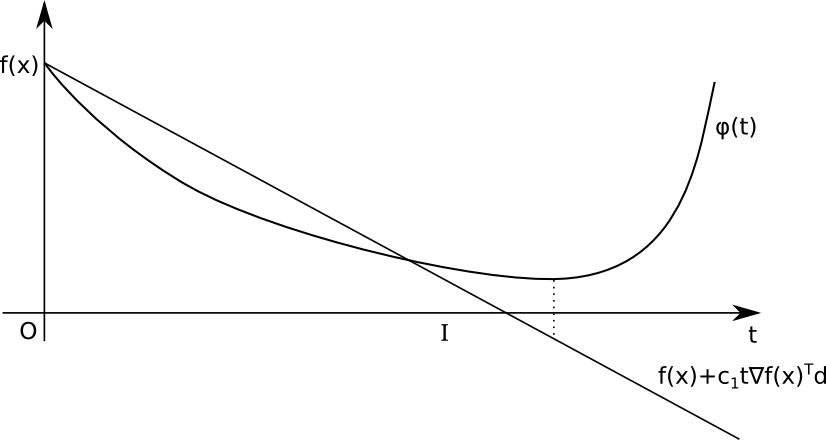
\includegraphics[width=0.60\textwidth]{imgs/ricerca-esatta-no-armijo.png}}

Perch\'e la condizione di Armijo valga per la ricerca esatta, la curva
di $\varphi(t)$, nel suo punto di minimo deve stare sotto la retta
$f(x) + c_1 t \nabla f(x)^{T}d$. Ma \`e possibile costruire degli
esempi, come quello del grafico, in cui questo non avviene.

Tuttavia, nella pratica $c_1$ viene scelto talmente piccolo (e dunque
la funzione lineare diventa talmente ``orizzontale'') che il minimo di
$\varphi(t)$ \`e sempre sotto.

Adesso poniamoci la domanda: esistono dei metodi che rispettino le
condizioni di Wolfe? Si può dimostrare che
\begin{proposition} Supponiamo $f$ sia inferiormente limitata. Allora
esiste un intervallo $(a,b)$ per cui le condizioni di Wolfe sono
verificate per ogni $t \in (a,b)$.

(Gli intervalli potrebbero essere anche pi\`u di uno.)
\begin{thproof} Sia
$$\tau_1= \sup \left\{ \tau ~ | ~  \forall ~ t \in [0, \tau]\ ~ \text{ \`e rispettata (AJO), ovvero } f(x^k + \tau_1 d^k) \leq f(x^k) + c_1 \tau_1 \nabla f(x^k)^T d^k \right\}$$
Vediamo alcune propriet\`a di questo insieme:
\begin{itemize}
\item Può l'insieme essere vuoto? Abbiamo visto in
\ref{prop:condizione-armijo-sempre-valida-in-intervallo} che la
condizione di Armijo vale almeno in un piccolo intervallo, quindi
l'insieme non \`e vuoto (esiste almeno un $\tau$).

\item Può il $\sup$ di questo insieme essere $+ \infty$? Se così
fosse, allora (AJO) varrebbe per ogni $t$, ma (AJO) vieta che $t$ vada
a $+\infty$ se la funzione \`e inferiormente limitata (si veda
\ref{prop:armijo-tk-non-infinito}). Quindi il $\sup$ deve essere un
numero finito.

\item Potremmo avere la disuguaglianza stretta?
$$ \underbrace{f(x^{k} + \tau_{1} d^{k})}_{\text{continua in }\tau_1} < \underbrace{f(x^{k}) + c_1 \tau_1 \nabla f(x^{k})^{T}d^{k}}_{\text{lineare in }\tau_1}$$
Se due funzioni continue in un punto non hanno lo stesso valore (caso
della disuguaglianza stretta), per il teorema della permanenza del
segno le due funzioni continuano ad essere una maggiore o uguale
dell'altra in tutto l'intorno del punto considerato. Ma allora questo
punto non sarebbe pi\`u il $\sup$, perch\'e la condizione continuerebbe a
valere in punti pi\`u grandi di $\tau_1$. Quindi abbiamo necessariamente
che
$$ f(x^{k} + \tau_{1} d^{k}) = f(x^{k}) + c_1 \tau_1 \nabla f(x^{k})^{T}d^{k}$$
\begin{equation}
\label{eq:esiste-intervallo-wolfe-no-disug-stretta} f(x^{k} + \tau_{1}
d^{k}) - f(x^{k}) = c_1 \tau_1 \nabla f(x^{k})^{T}d^{k}
\end{equation}
\end{itemize}

Per il teorema del valor medio, abbiamo
$$ f(x^{k} + \tau_{1} d^{k}) = \nabla f(x^{k} + \tau_2 d^{k})^{T} \cdot (\tau_1 d^{K}) = \tau_1 \nabla f(x^{k} + \tau_2 d^{k})^{T} d^{K}$$
per un opportuno $\tau_2 \in (0, \tau_1)$.

Ovvero, $x^k + \tau_2 d^k$ \`e un generico punto sul segmento che unisce
$x^{k}$ e $x^{k} + \tau_{1} d^{k}$:

\centerline{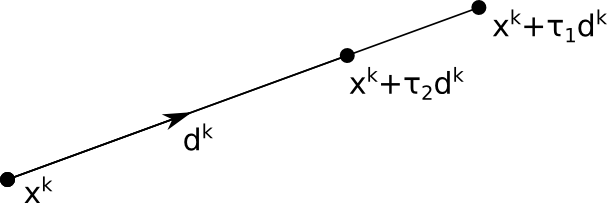
\includegraphics[width=0.30\textwidth]{imgs/passo-intermedio.png}}

Dato che $\tau_2 < \tau_1$, in $x^k + \tau_2 d^k$ vale al condizione
di Armijo. Dividiamo la
\ref{eq:esiste-intervallo-wolfe-no-disug-stretta} per $\tau_1$:

$$\nabla f(x^{k} + \tau_2 d^{k})^{T} d^{k} = c_1 \nabla f(x^{k})^{T} d^{K}$$
ma dato che $c_2 > c_1$ e $\nabla f(x^{k})^{T} d^{K} < 0$, \`e
$$f(x^{k} + \tau_2 d^{k})^{T} d^{k} = c_1 \nabla f(x^{k})^{T} d^{K} > c_2 \nabla f(x^{k})^{T} d^{K}$$

Abbiamo mostrato che nel punto individuato con il passo $\tau_2$ la
condizione (CUR) vale (con il maggiore stretto) e che in $[0, \tau_1]$
vale (AJO). Dunque, dato che $\nabla f$ \`e una funzione continua,
esiste un intervallo in cui valgono entrambe (la condizione di Wolfe \`e
rispettata):

\centerline{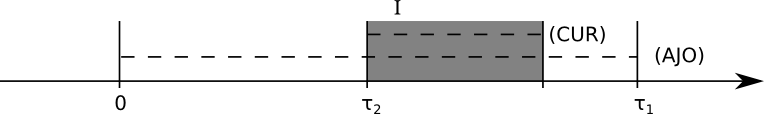
\includegraphics[width=0.60\textwidth]{imgs/intervallo-wolfe.png}}

\end{thproof}
\end{proposition}

Siamo in grado di sviluppare un algoritmo leggermente diverso dal
Metodo del Gradiente Esatto
(\ref{def:metodo-gradiente-esatto}). Funziona in modo simile ma con
due differenze: la direzione non \`e pi\`u necessariamente l'opposto del
gradiente ma \`e una generica direzione (passo
\ref{passo-algoritmo-gradiente-esatto-scelta-direzione}) e la ricerca
del passo di spostamento non \`e pi\`u esatta ma tale che le condizioni di
Wolfe (\ref{defn:condizioni-wolfe}) siano rispettate (passo
\ref{passo-algoritmo-gradiente-esatto-scelta-passo}).

\begin{defn}[Metodi del Gradiente con ricerca inesatta]
\label{def:metodo-gradiente-inesatto} Famiglia di metodi del gradiente
in cui si sceglie il passo con un metodo di ricerca inesatta.

Sotto forma di algoritmo si può enunciare come segue:
\begin{enumerate}
\item Poniamo $k=0$; Si sceglie un punto di partenza $x_0$;
\item Se $\nabla f(x^{k})=0$, allora STOP: abbiamo trovato un punto
stazionario.
\item \textbf{Si sceglie una direzione $d^k$ che sia di discesa (cio\`e
$\nabla f(x_k)^T d^k < 0$)}
\item \textbf{Calcolare $t_k > 0$ che soddisfi (AJO) e (CUR)}
\item Ci si sposta al punto successivo: $x^{k+1} = x^{k} + t_k \cdot
d^k$
\item $k:=k+1$, ritornare al passo
\ref{passo-algoritmo-gradiente-esatto-test-stop}.
\end{enumerate}

I metodi che rientrano in questa famiglia si differenziano per come
implementano la scelta della direzione (passo
\ref{passo-algoritmo-gradiente-esatto-scelta-direzione}) e per come
trovano il passo che soddisfi le condizioni di Wolfe (passo
\ref{passo-algoritmo-gradiente-esatto-scelta-passo}).
\end{defn}

\begin{notes} Il metodo del gradiente esatto rientra solo nella
pratica, e non formalmente, dentro questa famiglia di metodi
inesatti. Abbiamo visto infatti che sebbene la direzione $d^k = -
\nabla f (x^k)$ sia di discesa (\`e in effetti quella di massima
discesa, vedi \ref{subsection:massima-decrescita} a
pag. \pageref{subsection:massima-decrescita}), la ricerca esatta del
passo di spostamento non soddisfa in generale (ovvero per qualunque
valore di $c_1$ e per qualunque funzione da minimizzare) le condizioni
di Wolfe (vedi Propriet\`a
\ref{prop:passo-ricerca-esatta-soddisfa-wolfe}), ma le soddisfa
soltanto nella pratica scegliendo $c_1$ piccolo.
\end{notes}

\begin{notes} In realt\`a la dizione ``metodi del gradiente'' per i
metodi del gradiente con ricerca inesatta non \`e del tutto corretta,
perch\'e in questi metodi la direzione di spostamento non \`e
necessariamente scelta come l'opposto del gradiente, come avviene nel
Metodo del gradiente esatto (vedi
\ref{def:metodo-gradiente-esatto}). Tuttavia, questi metodi usano in
qualche modo il gradiente per scegliere la direzione quindi la dizione
può essere usata.
\end{notes}

Vogliamo adesso dimostrare la convergenza degli algoritmi che
appartengono a questa famiglia. Consideriamo le successioni $x^k$,
$d^k$ e $t_k$ generate da questa famiglia di metodi, e $ \theta_{k}$,
che \`e la successione dei valori dell'angolo compreso tra il gradiente
$\nabla f(x^{k})$ e la direzione $d^{k}$

\centerline{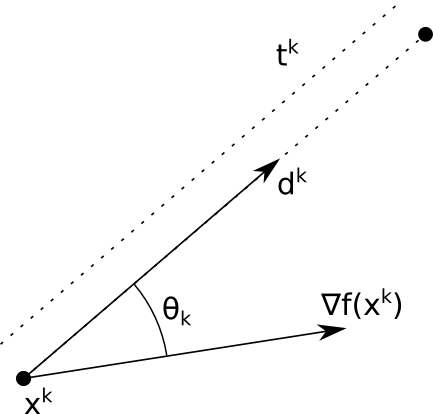
\includegraphics[width=0.25\textwidth]{imgs/dir-grad-theta.png}}

Le tre grandezze sono legate dalla seguente equazione, che avevamo gi\`a
incontrato in \ref{subsection:massima-decrescita}:
$$ \nabla f(x^{k})^{T} d^{K} = || \nabla f(x^{k}) ||_2 ||d^{k}||_2 \cos \theta_{k}$$

Vediamo innanzi tutto un lemma (che non dimostriamo)
\begin{lemma}
\label{lemma:lipschitziana-serie-convergente} Supponiamo che
 \begin{enumerate}
  \item $f$ sia inferiormente limitata
  \item $\nabla f$ non solo sia una funzione continua, ma che la
continuit\`a sia Lipschitziana (\ref{def:lipschitziana}), ovvero
      $$ \exists ~ L>0 \quad \text{t.c.} \quad \Vert \nabla f(x) - \nabla f(y) \Vert_{2} \leq L \Vert x - y \Vert_{2} \quad \forall ~ x,y \in \mathbb{R}^n$$
 \end{enumerate} Allora, detto $\theta_{k}$ l'angolo compreso tra $d_k$ e $\nabla f (x^k)$,
$$ \sum_{k=0}^{+\infty} \Vert \nabla f(x^{k}) \Vert_2^2 \cos^{2} \theta_{k} < + \infty$$
cio\`e la serie per $k= 0, \cdots, +\infty $ \`e convergente.
\end{lemma}

\begin{notes} Cosa significa dunque che una funzione \`e Lipschitziana?
Una funzione $f$ \`e continua quando per $y \to x \Longrightarrow \nabla
f(y) \to \nabla f(x)$. Una funzione Lipschitziana \`e continua, ma in
pi\`u dice con quale velocit\`a $L$ converge $\nabla f(y) \to \nabla
f(x)$.
\end{notes}
\begin{notes} Nel Lemma \ref{lemma:lipschitziana-serie-convergente} la
prima condizione nella pratica \`e soddisfatta sempre. Per quanto
riguarda la seconda, \`e in realt\`a necessario che sia soddisfatta solo
nelle vicinanze di un punto stazionario. Ad esempio, tutte le funzioni
polinomiali la soddisfano vicino ai punti stazionari.
\end{notes}

Del Lemma \ref{lemma:lipschitziana-serie-convergente} a noi non
interessa tanto la convergenza della serie, quanto piuttosto quello
che se ne può dedurre:

$$\sum_{k=0}^{+ \infty} ~ || \nabla f(x^{k}) ||_{2}^{2} \cos^{2} \theta_{k} < + \infty \quad \Longrightarrow \quad \Vert \nabla f(x^{k}) \Vert_{2}^{2} \cos \theta_{k} \longrightarrow_{k\rightarrow + \infty} 0$$

Questo risultato porta ad una dimostrazione immediata della
convergenza:

\begin{theo}[Convergenza] Se sono soddisfatte le ipotesi del Lemma
\ref{lemma:lipschitziana-serie-convergente}:
\begin{enumerate}
\item $f$ \`e inferiormente limitata
\item $\nabla f$ \`e Lipschitziana
\end{enumerate} e inoltre
\begin{enumerate}
\item[3.]$\exists ~ \delta > 0 \text{ t.c. } \cos \theta_{k} \leq
-\delta \quad \forall k$

(ovvero la successione dei $\cos\theta_k$ non sta andando a $0$,
quindi $\theta_k$ non può avvicinarsi pi\`u di tanto a
$\frac{\pi}{2}$. In altri termini, $\exists ~ \lambda \in
(0,\frac{\pi}{2}) \text{ t.c. } \theta_{k} \leq
\frac{\pi}{2}-\lambda$. Notare che $\theta_k$ lontano da
$\frac{\pi}{2}$ significa che il gradiente $\nabla f (x_k)$ e la
direzione $d_k$ non possono essere troppo ortogonali.)
\end{enumerate} Allora ogni punto di accumulazione della succesione
$\{x_k\}$ \`e un punto stazionario.

\begin{thproof} Abbiamo visto che per il Lemma
\ref{lemma:lipschitziana-serie-convergente},
$$\Vert \nabla f(x^{k}) \Vert_{2}^{2} \cos \theta_{k} \longrightarrow_{k\rightarrow + \infty} 0$$
Ma con l'ipotesi 3 abbiamo anche impedito che $\cos \theta_{k}$
vada a zero (il punto pi\`u vicino a zero che il limite può raggiungere
\`e $-\delta$), dunque non può che essere:
$$ \Vert \nabla f(x^{k})\Vert^{2}_{2} \longrightarrow_{k \to +\infty} 0 \quad \Longleftrightarrow \quad \Vert \nabla f(x^{k})\Vert_{2} \longrightarrow_{k \to +\infty} 0$$
ma se la norma del gradiente tende a zero per qualunque
sottosuccessione, questo vale in particolare per la sottosuccessione
che tende al punto di accumulazione. Passando al limite, per la sua
unicit\`a si ha:
$$\Vert \nabla f (x^*) \Vert_2 = \lim_{k \to +\infty} \Vert \nabla f(x^k) \Vert_2 = 0$$
abbiamo dimostrato che
$$\Vert \nabla f (x^*) \Vert_2 = 0$$
\end{thproof}
\end{theo}

%\subsection{Esempi al calcolatore}
%$$ f(x_1,x_2) = x_1^2 + 5x_2^{2} $$
%$x^{*}=(0,0)$ \\ %Possiamo applicare il metodo del gradiente esatto.
%Essendo la funzione quadratica il passo può essere calcolato
%esplicitamente.
%
%$$
%Q= \begin{pmatrix} % 2 & 0\\ % 0 & 10
%\end{pmatrix} %\quad %b = \begin{pmatrix} % 0 \\ % 0
% \end{pmatrix} %\quad %c = 0
%$$
%
%$$ f(x) = \frac{1}{2} x^{T} Qx + b^{T} x + \not{c}$$
%Condizioni di arresto
%$$ || \nabla f(x^{k})||_{2} \leq \epsilon $$
%$$ || x^{k+1} - x^{k} ||_{2} \leq \epsilon'$$
%Di solita si usa $10^{-6}$.\\ %Usando il punto $(0,2)$ come punto di
%partenza, %si ha convergenza in un solo colpo, ottenendo la soluzione
%esatta. \\ %Mammano che ci avvicina alla soluzione si converge sempre
%pi\`u lentamente. \\ %L'algoritmo ha eseguito 24 iterazioni.  %La
%direzione viene cambiata quando si va tangenti al gradiente (curve di
%livello).\\ %La ricerca inesatta non \`e detto che sia pi\`u veloce, ma
%in termini di risorse computazionali \`e pi\`u efficiente.
%\paragraph{Esempio rifrazione} %In questo problema abbiamo una
%funzione a due variabili. \\ % non abbiamo una funzione quadratica,
%dobbiamo %dobbiamo risolvere un problema di ottimizzazione.
%
%\paragraph{Rosenbrock}
%$$ f(x_1,x_2) =  100(x_2  - x_1^{2})^{2} + (1-x_1)^{2}$$
%$x^{*} = (0,0)$ %Funzione difficile per il gradiente esatto,
%convergenza molto lenta.  %1296 passi per la convergenza. Il problema
%\`e che le curve di %livello sono a banana. Quale che sia il punto di
%partenza, si %va a soffrire sempre di questo problema.

\subsection{Metodo di Netwon-Raphson} Negli esperimenti, si \`e visto
che per alcune funzioni il Metodo del gradiente esatto \`e molto
lento. Ad esempio, per la funzione di Rosenbrock
(\ref{eq:rosenbrok-banana} a pag. \pageref{eq:rosenbrok-banana}), per
ottenere un risultato con un'approssimazione di $10^{-6}$ sono
necessarie pi\`u di 1000 iterazioni. Un metodo del gradiente con ricerca
inesatta non si comporterebbe meglio per via della conformazione della
funzione.

Ma, come abbiamo visto, non \`e obbligatorio muoversi in direzione del
gradiente. Si possono usare altri strumenti, ad esempio il metodo di
Newton-Raphson (trattato nella Sezione \ref{section:metodo-newton-raphson}),
che serve per risolvere un sistema di equazioni non lineari $F$:
$$ F:\mathbb{R}^{n} \rightarrow \mathbb{R}^n$$
per trovare un $x^*$ tale che
$$ F(x^*) =0$$
Il metodo iterativo gi\`a visto nella Sezione
\ref{section:metodo-newton-raphson} \`e

\begin{equation}
\label{eq:metodo-iterativo-newton} x^{k+1} = x^{k} - [JF(x^{k})]^{-1}
F(x^{k})
\end{equation} dove $JF(k^x)$ \`e la matrice Jacobiana di $F$ calcolata
in $x^k$. Ovvero, dopo aver ottenuto un punto $x^k$, quello successivo
si sceglie muovendosi lungo la direzione $-JF(x^k)^{-1}\cdot F(x^k)$
di passo unitario.

Si nota una forte somiglianza con i metodi di discesa visti finora:
anche in Newton-Raphson, dato un punto, ci si muove lungo una certa
direzione calcolata in funzione del punto stesso.

Possiamo usare questo metodo, che trova gli zeri di una funzione, per risolvere il
nostro problema, ovvero:
$$ \text{(P)}\qquad \min\{f(x): x \in \mathbb{R}^{n} \} \quad f: \mathbb{R}^{n} \rightarrow \mathbb{R} \quad \nabla f: \mathbb{R}^{n} \rightarrow \mathbb{R}^{n}$$
Infatti per risolvere (P) è necessario trovare i punti stazionari, ovvero $x$ tale che $ \nabla f(x) = 0$. Possiamo dunque usare il metodo di Newton--Raphson ponendo:
$$ F = \nabla f$$
per cercare $x \text{ t.c. } F(x) = \nabla f(x) = 0$

Ma cosa \`e la matrice jacobiana della funzione gradiente? Ricordando
che il gradiente \`e
$$\nabla f(\overline{x}) = \left(
\begin{array}{c}\frac{\partial f}{\partial x_1}\\ \frac{\partial
f}{\partial x_2}\\ \vdots\\ \frac{\partial f}{\partial x_n}
\end{array} \right)$$

La matrice jacobiana \`e la matrice delle derivate parziali delle $n$
funzioni, quindi bisogna derivare $\frac{\partial f}{\partial x_i}$
rispetto a $x_i$. Quindi stiamo semplicemente derivando due volte
(ottenendo la matrice hessiana).

$$J(\nabla f)(x) = \nabla^{2} f(x) $$

e il metodo di Newton-Raphson in \ref{eq:metodo-iterativo-newton}
diventa
$$ x^{k+1} = x^{k} - [ \nabla^{2}f(x^{k})]^{-1} \nabla f(x^{k})$$

Questo metodo rientra nella classe dei metodi del gradiente inesatto
(vedi \ref{def:metodo-gradiente-inesatto}), con passo e direzione

\begin{equation}
\label{newtongradesatto}
 t^k = 1 \qquad d^{k} = -[\nabla^{2} f (x^{k})]^{-1} \nabla f(x^{k})
\end{equation}
\begin{notes} Nel paragrafo sulle Direzioni alternative di decrescita
(pag. \pageref{par:direzioni-alternative-decrescita}) avevamo parlato
della possibilit\`a di scegliere la direzione $d_k$ perturbando la
direzione del gradiente con una generica matrice $D_k$. In questo
caso, abbiamo scelto $D_k=[ \nabla^{2}f(x^{k})]^{-1}$.
\end{notes}

\paragraph{Convergenza: Vogliamo la direzione di discesa, ma a che
costo!}  In questo paragrafo, vedremo quali condizioni devono essere
soddisfatte affich\'e il metodo sia di discesa, e vedremo che queste
condizioni sono molto strette, così nel prossimo paragrafo vedremo che
questo vincolo può essere rilassato, e si può avere un metodo che non
sempre converge.

Come possiamo garantire che al passo $k$ la direzione $d^k$ sia di
discesa? Nel paragrafo sulle direzioni di decrescita
(pag. \pageref{par:direzioni-alternative-decrescita}) avevamo visto
che se $D_k$ \`e definita positiva, allora la direzione $d^k$ \`e di
discesa. Quindi nel nostro caso, se la matrice hessiana \`e definita
positiva, allora la sua matrice inversa \`e definita positiva e le
direzioni $d^k$ sono sempre di discesa.

Dato che in tutti i punti $x_k$ della successione la matrice hessiana
deve essere definita positiva, l'unico modo per avere la garanzia che
il metodo sia di discesa, \`e che la matrice hessiana sia definita
positiva in ogni punto. Ma se la matrice hessiana \`e definita positiva
in ogni punto allora la funzione \`e strettamente convessa.

Dunque chiedere che il metodo sia di discesa equivale a limitare
l'algoritmo a risolvere solo funzioni strettamente convesse, e
neanche tutte: vi sono infatti delle funzioni strettamente convesse la
cui hessiana non \`e sempre definita positiva. Evidentemente, questo
risultato \`e troppo limitante.

\paragraph{Convergenza: \`E necessario che la direzione sia di discesa?}
Proviamo a rilassare le nostre richieste: a noi non serve che il
metodo sia sempre di discesa, l'importante \`e che converga ad un punto
stazionario.

Abbiamo visto nel Teorema di convergenza del metodo Newton-Raphson
\ref{theo:convergenza-newton-raphson} (pag. \pageref{theo:convergenza-newton-raphson}) che se $F$ (ovvero ognuna delle
sue componenti) \`e differenziabile 2 volte con continuit\`a e data una
soluzione $x^*$ tale che $f(x^*) =0$, allora se $JF(x^{*})$
\`e invertibile e il metodo parte da un punto $x^0$
sufficientemente vicino alla soluzione, il metodo converge.

% e converge con la propriet\`a
%$$ \exists  ~ M > 0 \text{ t.c. }|| x^{k+1} - x^{*}||_{2} \leq M||x^{k} - x^{*}||_{2}^{2} $$
%ovvero ad una certa iterazione, la distanza dalla soluzione \`e
%limitata dalla distanza all'iterazione precedente al quadrato.

Abbiamo visto nel paragrafo precedente che al passo $k$, se la matrice hessiana $\nabla^2 f(x^k)$ \`e
definita positiva, allora la direzione \`e di discesa.

Guardiamo cosa succede se nelle
ipotesi del Teorema \ref{theo:convergenza-newton-raphson} aggiungiamo il fatto che la
matrice hessiana $\nabla^2f(x)$ sia definita positiva nel punto
stazionario.

Si noti che se una matrice \`e definita positiva allora \`e anche
invertiblile, quindi abbiamo chiesto anche che $\nabla^2f(x) =
J(\nabla f)(x^{*}) = JF(x^{*})$ sia invertibile, le ipotesi del
teorema restano quindi soddisfatte, e dunque il metodo converge a $x^*$.

Oltre a convergere, l'ipotesi che abbiamo aggiunto ci dà la garanzia che il metodo, una volta entrato nell'intorno di $x^*$, sia di discesa. Si ricorda che, perché questo sia verificato, $D^k$ deve essere definita positiva ad ogni iterazione. E questo è verificato perché se la matrice hessiana \`e definita positiva in $x^*$,
allora \`e definita positiva anche in un suo intorno\footnote{Questo
perch\'e abbiamo scelto $\nabla^2 f(x)$ derivabile 2 volte con continuità.}.

%Questo significa che alle prime iterazioni il metodo potrebbe
%divergere, ma dato che converge, definitivamente dovr\`a entrare
%nell'intorno di $x^*$ in cui $\nabla^2 f(x)$ \`e definita positiva e il
%metodo diventer\`a di discesa.

Queste considerazioni ci permettono di riscrivere il teorema in
maniera diversa, nel contesto dell'ottimizzazione.

\begin{theo}
\label{theo:convergenza-newton-raphson-ottimizzazione} Se
\begin{enumerate}
\item $f$ \`e differenziabile 3 volte con continuit\`a;
\item $x^{*} \in \mathbb{R}^{n}$ \`e punto stazionario di $f$ tale che
$\nabla^{2} f(x^{*})$ \`e definita positiva.
\end{enumerate} Allora, per il Teorema
\ref{theo:convergenza-newton-raphson},
$$\exists~ \delta > 0 \quad \text{t.c.}\quad \forall x^{0} \in B(x^{*},\delta), x^{k} \rightarrow x^{*}$$
(il metodo converge) e inoltre

$\exists M > 0 $ per cui:
$$|| x^{k+1} -x^{*}||_{2} \leq M ||x^{k} - x^{*}||_{2}^{2}$$
(la convergenza è superlineare)
\end{theo}

Applicando il metodo di Newton-Raphson al nostro problema di
minimizzazione abbiamo ottenuto il teorema appena
enunciato. Confrontiamolo con l'originale Teorema di convergenza del
metodo Newton-Raphson \ref{theo:convergenza-newton-raphson}. Le
conclusioni sono le stesse, così come la seconda ipotesi. Per quanto
riguarda la prima ipotesi, il metodo originale chiede che $F$ sia
differenziabile 2 volte con continuit\`a, ma nel nostro caso $F=\nabla
f$ e quindi la prima ipotesi equivale a chiedere che $f$ sia
differenziabile 3 volte con continuit\`a.

\paragraph{Propriet\`a del metodo} Facciamo alcune osservazioni su
questo metodo, cominciando dal punto stazionario $x^*$.
\begin{observation} Abbiamo chiesto che $f(x^*)=0$ e che $\nabla^2 f
(x^*)$ sia definita positiva. Dal Teorema
\ref{theo:punto-stazionario-minimo-locale} sappiamo che queste sono le
condizioni sufficienti affinché $x^*$ sia un punto di minimo locale.
\end{observation}

Sul punto di partenza $x_0$:
\begin{observation} Nei metodi visti in precedenza, non ci eravamo
preoccupati della scelta del punto di partenza, che poteva essere uno
qualunque, garantendo la convergenza. In Newton-Raphson invece non può
essere scelto a caso ma deve essere tale che $x^{0} \in
B(x^{*},\delta)$, ovvero che non sia troppo lontano dalla soluzione. \`E
un metodo di natura locale, e se non si ha idea di dove sia il punto
di minimo può darsi che le ipotesi non siano verificate e dunque il
metodo non converga o converga a un punto stazionario che però \`e un
punto di massimo oppure un punto né di minimo né di massimo.
\end{observation}

\begin{observation} Il passo $t_k$ \`e identicamente 1 (e la
dimostrazione della convergenza \`e basata su questo). É possibile
modificare il metodo di newton perch\'e esegua una ricerca esatta o
inesatta.
\end{observation}

\begin{observation} Il calcolo \`e oneroso, infatti ad ogni iterazione
il calcolo della direzione ha bisogno del calcolo della matrice
hessiana e della sua inversa.

Proprio per questo ci sono dei metodi, chiamati para--Newton, che
invece di calcolare esattamente $\nabla^2f(x)$ ne calcolano
un'approssimazione. Ad ogni iterazione, la matrice non viene
ricalcolata ma aggiornata tramite una formula esplicita che stima la
variazione di questa matrice rispetto al suo valore nel passo
precedente in funzione del valore del gradiente. (In una dimensione,
questo equivale a stimare la variazione della derivata seconda in base
al valore della derivata nel punto.)
\end{observation}

\paragraph{Un'altra derivazione del metodo di Newton} Nel paragrafo
precedente, abbiamo preso il metodo di Newton da un altro contesto
(originariamente serviva per trovare gli zeri di una funzione) e lo
abbiamo applicato al campo dell'ottimizzazione. Per capire meglio il
suo funzionamento, proviamo ad ottenerlo dal contesto
dell'ottimizzazione, partendo stavolta dagli sviluppi di Taylor.

Si ricorda che col metodo del gradiente prendevamo una funzione nel
punto $x+d$ che si approssimava al primo ordine con
$$f(x + d) \approx f(x) + \nabla f(x)^{T} d$$
Nell'approssimazione vengono scartati i termini del secondo
ordine. Cercando di minimizzare questa quantit\`a, data la necessit\`a di
limitare $\Vert d \Vert$ ad un valore finito, si otteneva che doveva
essere $d=-\nabla f(x)$. Dunque sviluppando al primo ordine si ottiene
il metodo del gradiente.

Ma che succede se sviluppiamo al secondo ordine? Innanzi tutto la
funzione $f$ deve essere derivabile 2 volte. Si ottiene:
$$f(x + d) \approx f(x) + \nabla f(x)^{T} d + \frac{1}{2} d^{T} \nabla^2 f(x)d = m_2(d)$$
(in questo caso scartiamo i termini di ordine 3)

Come prima, vogliamo minimizzare questa funzione $m_2$,
approssimazione al secondo ordine di $f$. Ma $m_2$ \`e una funzione
quadratica:

$$ m_2(d) = \frac{1}{2} d^{T} \underbracket{\nabla^2 f(x)}_{Q}d + \underbracket{\nabla f(x)}_{b} {^T} d + \underbracket{f(x)}_{c}$$

Sappiamo che se $\nabla^2 f(x)$ non \`e semidefinita positiva, la
funzione non ha limite inferiore. Quindi supponiamo che sia
semidefinita positiva. Se \`e semidefinita positiva, allora $m_2(d)$ \`e
convessa. E se $m_2$ \`e convessa, significa che tutti i punti
stazionari sono anche punti di minimo.

Calcoliamo il gradiente della funzione
quadratica\footnote{Dall'Osservazione
\ref{obs:gradiente-hessiana-funzione-quadratica} si ha che con $f$
quadratica, si ha $\nabla f(x) = Qx + b$ e $\nabla^2 f(x) = Q$} e
cerchiamo dove si annulla:
$$ \nabla m_2(d) \defeq \nabla^{2} f(x) d + \nabla f(x)=0$$
Si forma quindi il sistema lineare:
$$ \nabla^{2} f(x) d = - \nabla f(x)$$
Se la matrice hessiana \`e invertibile (ad esempio, se $\nabla^{2} f(x)$
\`e definita positiva\footnote{Finora abbiamo supposto solo che fosse
semi--definita positiva.}), allora il sistema si risolve con:
$$ d = - [\nabla^2f(x) ]^{-1} \nabla f(x)$$

Che \`e proprio la direzione usata nel metodo di Newton! Cosa significa
questo? che la direzione del metodo di Newton \`e quella che minimizza
lo sviluppo al secondo ordine della funzione $f$ (sviluppata intorno
al punto $x$).

\begin{observation} Quando \`e che l'approssimazione del secondo ordine
usata dal metodo di Newton \`e buona? Quando $\Vert d \Vert$ \`e molto
piccola. Guardiamo infatti lo sviluppo di Taylor del \emph{primo}
ordine non approssimato ma con il resto esatto:
$$ f(x+d) = f(x) + \nabla f(x)^{T}d+ \frac{1}{2} d^{T} \nabla^{2} f(x+td)d
\quad t\in(0,1)$$ (Rispetto allo sviluppo del secondo ordine
approssimato, la matrice hessiana non \`e calcolata nel punto $x$ ma nel
punto intermedio tra $x$ e $x+d$, ovvero $x+td$ con $t\in(0,1)$.)

La sola differenza tra lo sviluppo esatto e quello inesatto \`e tra
$\nabla^{2} f(x+td)d$ e $\nabla^{2} f(x)d$ che ovviamente convergono
per $d \to 0$ e in particolare si avvicinano se le derivate seconde
per le componenti sono piatte.
\end{observation}

\begin{observation} Il Teorema
\ref{theo:convergenza-newton-raphson-ottimizzazione} fornisce anche la
velocit\`a di convergenza: la propriet\`a secondo cui $\exists M > 0 $ per
cui:
$$|| x^{k+1} -x^{*}||_{2} \leq M ||x^{k} - x^{*}||_{2}^{2}$$

si chiama convergenza superlineare del secondo ordine (si può vedere
che il Metodo del gradiente ha convergenza lineare).
\end{observation}

\paragraph{Applicazioni del metodo di Newton} Abbiamo appena visto che
il metodo di Newton minimizza una versione quadratica della funzione
obiettivo. Se applicassimo il metodo di Newton ad una funzione
quadratica, l'approssimazione sarebbe senza errore. Quindi la
convergenza si ottiene in un solo passo.

\begin{exercise} Si applichi il metodo di Newton alla funzione
$f(x)=x_1^2 + 5\cdot x_2^2$ con un punto di partenza qualunque.
\end{exercise}

\begin{observation} Cosa succede se si applica il metodo alla funzione
banana di Rosenbrock \ref{eq:rosenbrok-banana}? Come abbiamo visto, il
punto iniziale deve essere sufficientemente vicino alla soluzione, che
in questo caso come sappiamo \`e $x^* = (1,1)$.
\begin{itemize}
\item Se si parte da $x_0 = (1.1,1.1)$ il metodo diverge, perch\'e la
partenza \`e troppo lontana dalla destinazione. Infatti la matrice
hessiana calcolata in $x^*$ \`e positiva, però, calcolata nel punto di
partenza $x_0$ abbiamo un autovalore negativo, quindi la prima
iterazione non \`e di discesa e neanche quelle successive.
\item Con $x_0 = (1.01,1.01)$ continua a divergere.
\item Con $x_0 = (1.001,1.001)$ finalmente il metodo converge perch\'e
la matrice hessiana in $x_0$ \`e definita positiva.
\end{itemize}
\end{observation}

\outbpdocument

%%% Local Variables: 
%%% mode: latex
%%% TeX-master: "appunti"
%%% End: 
 %% Bigi: ottimizzazione non vincolata
 %% Copyright (C) 2011, Andrea Cimino, All Rights Reserved.
 %% This file is distributed under the terms of the Creative Commons
 %% Licence Non-Commercial Share-Alike license

%% Useful stuff for separate compilation.
\ifx\ismaindoc\undefined
\providecommand{\inbpdocument}{
 \documentclass[11pt,a4paper,twoside,titlepage]{scrbook}
%%%%%%%%%%%%%%%%%%%%%%%%%%%%%%%%
%%%%%%%%%%% PACKAGES %%%%%%%%%%%
%%%%%%%%%%%%%%%%%%%%%%%%%%%%%%%%
% encoding
\usepackage[utf8x]{inputenc}
\usepackage[italian]{babel} % babel (suddivisione parole in sillabe)

\usepackage{amsfonts} % matematica
\usepackage{amsmath} % matematica
\usepackage{amssymb} % simboli vari
\usepackage{calrsfs}
\usepackage{caption}
\usepackage{enumerate}
\usepackage{extarrows} % matematica
\usepackage{keyval}
\usepackage{manfnt} % Simboli curva
\usepackage{mathtools} % matematica
\usepackage{multirow} 
\usepackage[usenames, dvipsnames]{color} % colori con nome
\usepackage[pdftex]{graphicx}
\usepackage{epstopdf} % gestione file EPS
\usepackage{wrapfig} % per figure circondate da testo
\usepackage{framed}	% teoremi framed
\usepackage{fancyhdr} % header buffi
\usepackage[T1]{fontenc} % gestione hbox e vbox
\usepackage[a4paper]{geometry}
\usepackage{microtype} % gestione hbox e vbox
\usepackage[thref, amsthm, amsmath, framed, hyperref]{ntheorem} % teoremi (avanzata)
%% \usepackage{prooftree} % gestione prof-tree
\usepackage{rotating}
\usepackage{stmaryrd}
\usepackage{subfig}
\usepackage{syntax} % syntattic stuff
\usepackage{txfonts}
\usepackage{verbatim} % migliorie al verbatim
%\usepackage{hyperref}
%% \usepackage{qtree}
\usepackage{fancyvrb}
\usepackage{listings}
\usepackage{cancel}
\usepackage{tikz}

\usepackage{bbding} %% Icons

%%%%%%%%%%%%%%%%%%%%%%%%%%%%%%%%
%%%%%%%%%%% GEOMETRY %%%%%%%%%%%
%%%%%%%%%%%%%%%%%%%%%%%%%%%%%%%%
\geometry{verbose,tmargin=2cm,bmargin=2.5cm,lmargin=2.5cm,rmargin=2cm}
\parindent0ex %% Remove paragraph indenting

%%%%%%%%%%%%%%%%%%%%%%%%%%%%%%%%
%%%%%%%%%%% CODE ENV %%%%%%%%%%%
%%%%%%%%%%%%%%%%%%%%%%%%%%%%%%%%
% codice
\newcounter{count}
\setcounter{count}{0}
\newenvironment{code}[1]
{
\color{lightgray}\hrulefill\color{code}
\stepcounter{count} {\bf\small Listato di codice \arabic{count}: {#1} }
\verbatim
}
{
\endverbatim
\color{lightgray}\hrulefill
\color{black}
\\
}

% codice semplice
\newenvironment{simplecode}
{
\color{code} \tt
}
{
\rm
}

 % Notation issues
\input{macros}

\makeatletter
\g@addto@macro\@verbatim\footnotesize
\makeatother



%%%%%%%%%%%%%%%%%%%%%%%%%%%%%%%%
%%%%%%%% THEOREMS FORMAT %%%%%%%
%%%%%%%%%%%%%%%%%%%%%%%%%%%%%%%%
% shaded theorems and proofs command
\definecolor{lightgray}{RGB}{230,230,230}
\def\theoremframecommand{\colorbox{lightgray}}

%%% theorems
\theoremstyle{break}
\theoremheaderfont{\normalfont\bfseries}
\theorembodyfont{\itshape}
\theoremsymbol{\ensuremath{\diamondsuit}}
\theoremseparator{\newline}
\newtheorem{theo}{
\includegraphics[scale=0.11]{imgs/book.png}Teorema}[chapter]

%%% propositions
\theoremstyle{break}
\theoremheaderfont{\normalfont\bfseries}
\theorembodyfont{\itshape}
\theoremsymbol{\ensuremath{\diamondsuit}}
\theoremseparator{\newline}
\newshadedtheorem{proposition}{Proposizione}[chapter]

%%% exercises
\theoremstyle{break}
\theoremheaderfont{\normalfont\bfseries}
\theorembodyfont{\itshape}
\theoremsymbol{\ensuremath{\diamondsuit}}
\theoremseparator{\newline}
\newshadedtheorem{exercise}{Esercizio}[chapter]

%%% propositions
\theoremstyle{break}
\theoremheaderfont{\normalfont\bfseries}
\theorembodyfont{\itshape}
\theoremsymbol{\ensuremath{\diamondsuit}}
\theoremseparator{\newline}
\newshadedtheorem{property}{\PencilRightDown $\; $ Propriet\`a}[chapter]

%%% lemmas
\theoremstyle{break}
\theoremheaderfont{\normalfont\bfseries}
\theorembodyfont{\itshape}
\theoremsymbol{\ensuremath{\diamondsuit}}
\theoremseparator{\newline}
\newshadedtheorem{lemma}[theo]{Lemma}

%%% definitions
\theoremstyle{break}
\theoremsymbol{\ensuremath{\clubsuit}}
\theoremseparator{\newline}
\newshadedtheorem{defn}[theo]{Definizione}

%%% examples
\theoremstyle{break}
\theorembodyfont{\itshape}
\theoremsymbol{\ensuremath{\ast}}
\theoremseparator{\newline}
\newshadedtheorem{example}[theo]{Esempio}

%%% observations
\theoremstyle{break}
\theorembodyfont{\itshape}
\theoremsymbol{\ensuremath{\ast}}
\theoremseparator{\newline}
\newshadedtheorem{observation}[theo]{

\includegraphics[scale=0.06]{imgs/lens.png}
Osservazione
}

%%% notations
\newtheorem*{notaz}{Notazione}

%%% proofs
\newenvironment{thproof}
{
\vskip 0.03cm
\begin{small}
\textit{Dimostrazione. }
\color{code}
}
{
\color{black}
\end{small}
$ \square $
\vskip 0.2cm
}

%Notes
\newenvironment{notes}{%
  \def\FrameCommand{\colorbox{yellow}}%
  \MakeFramed {\FrameRestore}
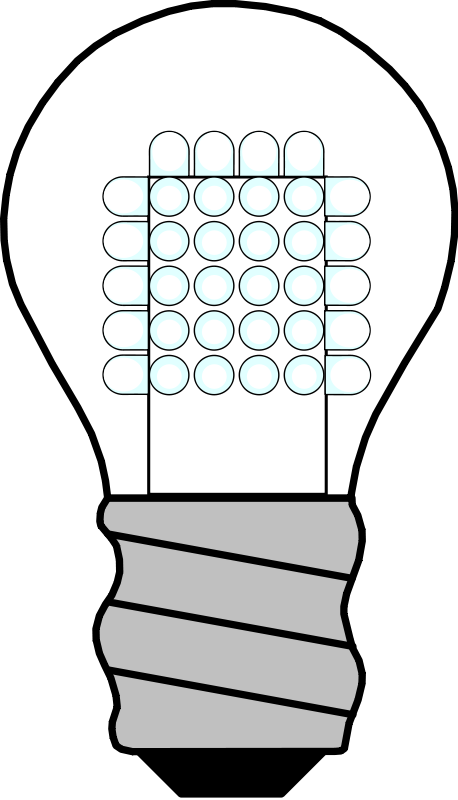
\includegraphics[scale=0.02]{imgs/bulb.png}
 \textbf{Nota} \\
 }%
{\endMakeFramed}

%Work in progress
\newenvironment{workinprogress}{%
  \def\FrameCommand{\colorbox{pink}}%
  \MakeFramed {\FrameRestore}
\lhdbend  \textbf{Work in progress} \\
 }%
{\endMakeFramed}

%Openquestion
\newenvironment{openquestion}{%
  \def\FrameCommand{\colorbox{pink}}%
  \MakeFramed {\FrameRestore}
 \textbf{Domanda aperta} \\
 }%
{\endMakeFramed}

%TODO
\newenvironment{todo}{%
  \def\FrameCommand{\colorbox{pink}}%
  \MakeFramed {\FrameRestore}
 \textbf{TODO} \\
 }%
{\endMakeFramed}

%%%%%%%%%%%%%%%%%%%%%%%%%%%%%%%%
%%%%%%%%%%%% HEADER %%%%%%%%%%%%
%%%%%%%%%%%%%%%%%%%%%%%%%%%%%%%%
\pagestyle{fancy}
% i comandi seguenti impediscono la scrittura in maiuscolo
% dei nomi dei capitoli e dei paragrafi nelle intestazioni
\renewcommand{\chaptermark}[1]{\markboth{#1}{}}
\renewcommand{\sectionmark}[1]{\markright{\thesection\ #1}}
\fancyhf{} % rimuove l'attuale contenuto dell'intestazione
% e del pi\`e di pagina
\fancyhead[LE,RO]{\bfseries\thepage}
\fancyhead[LO]{\bfseries\rightmark}
\fancyhead[RE]{\bfseries\leftmark}
\renewcommand{\headrulewidth}{0.5pt}
\renewcommand{\footrulewidth}{0pt}
\addtolength{\headheight}{0.5pt} % riserva spazio per la linea
\fancypagestyle{plain}{%
\fancyhead{} % ignora, nello stile plain, le intestazioni
\renewcommand{\headrulewidth}{0pt} % e la linea
}


%%%%%%%%%%%%%%%%%%%%%%%%%%%%%%%%
%%%%%%%%%%%% COLORS %%%%%%%%%%%%
%%%%%%%%%%%%%%%%%%%%%%%%%%%%%%%%
\definecolor{code}{gray}{0.3}


%%%%%%%%%%%%%%%%%%%%%%%%%%%%%%%%
%%%%%%%%%%%% NUMBERS %%%%%%%%%%%
%%%%%%%%%%%%%%%%%%%%%%%%%%%%%%%%
\setcounter{tocdepth}{3}
\setcounter{secnumdepth}{3}


%%%%%%%%%%%%%%%%%%%%%%%%%%%%%%%%
%%%%%%%%%%% DOC DATA %%%%%%%%%%%
%%%%%%%%%%%%%%%%%%%%%%%%%%%%%%%%
\title{Appunti di MNO}
\author{Gruppo Informatici Rampanti}
\date{ott 2010 - mag 2011}

\pdfinfo{%
  /Title    (Appunti di MNO)
  /Author   (Andrea Cimino e Lorenzo Muti)
  /Creator  (Andrea Cimino)
  /Producer (Lorenzo Muti)
  /Subject  (MNO)
  /Keywords (MNO)
}


%%%%%%%%%%%%%%%%%%%%%%%%%%%%%%%%
%%%%%%%%%%%%% UTILS %%%%%%%%%%%%
%%%%%%%%%%%%%%%%%%%%%%%%%%%%%%%%
% binary symbols
\newcommand{\modder}{\vdash _{R}}

% vertical gaps
\newcommand{\askip}{\vspace{0.5cm}}
\newcommand{\bskip}{\vspace{1.0cm}}

% various symbols
\newcommand{\qedhere}{\ensuremath{\Box}}
\newcommand{\qed}{\hfill \ensuremath{\Box}}

% substitution
\newcommand{\subst}[2]{^{#1} / _{#2}}

% denotational semantics function names
\newcommand{\bbracket}[1]{\left\llbracket #1 \right\rrbracket}

\newcommand{\aexpr}{\mathcal{A}}
\newcommand{\bexpr}{\mathcal{B}}
\newcommand{\cexpr}{\mathcal{C}}
\newcommand{\Aexpr}[1]{\mathcal{A} \bbracket{#1}}
\newcommand{\Bexpr}[1]{\mathcal{B} \bbracket{#1}}
\newcommand{\Cexpr}[1]{\mathcal{C} \bbracket{#1}}

\newcommand{\semdomset}[1]{(V_{#1})_{\bot}}

% semantic evaluations
\newcommand{\opereval}[3]{\left\langle #1, #2 \right\rangle \rightarrow #3}
\newcommand{\denaeval}[3]{\Aexpr{#1} #2 = #3}
\newcommand{\denbeval}[3]{\Bexpr{#1} #2 = #3}
\newcommand{\denceval}[3]{\Cexpr{#1} #2 = #3}

% rotated sqsubseteqs
\newcommand{\upsqsubseteq}{ $\begin{rotate}{90} $\sqsubseteq$ \end{rotate}$ }
\newcommand{\downsqsubseteq}{ $\begin{rotate}{270} $\sqsubseteq$ \end{rotate}$ }

% Space after paragraph declaration
\makeatletter
\renewcommand\paragraph{\@startsection{paragraph}{4}{\z@}%
  {-3.25ex\@plus -1ex \@minus -.2ex}%
  {1.5ex \@plus .2ex}%
  {\normalfont\normalsize\bfseries}}
\makeatother



% fast theorem and definition
\newcommand{\ftheo}[1]{\colorbox{YellowGreen}{#1}}
\newcommand{\fdefn}[1]{\colorbox{SkyBlue}{#1}}

\theoremstyle{break}
\theoremsymbol{\ensuremath{\clubsuit}}
\theoremseparator{\newline}
\newshadedtheorem{proc}[theo]{Procedura}

% bold math!
\newcommand{\bm}[1]{\mbox{\boldmath{$#1$}}}

\newcommand{\positive}[1]{\textbf{\color{green} +} #1}
\newcommand{\negative}[1]{\textbf{\color{red} -} #1}


\newtheoremlisttype{tab}%
{\begin{tabular*}{\linewidth}{@{}lrl@{\extracolsep{\fill}}r@{}}}%
{##1&##2&##3&##4\\}%
{\end{tabular*}}
\begin{document}
}
\providecommand{\outbpdocument}{\end{document}}
\else
\providecommand{\inbpdocument}{}
\providecommand{\outbpdocument}{}
\fi



\inbpdocument 

%% 21 Gennaio
\chapter{Metodo del gradiente coniugato}
\label{chap:metodo-gradiente-coniugato}
\section{Motivazioni e strumenti} Il metodo del gradiente coniugato \`e
un metodo iterativo per risolvere $Ax = b$, che ha una proprietà:
converge in al più $n$ passi dove $n$ \`e l'ordine della matrice $A$.\\
Per avere la convergenza veloce si sfruttano delle ipotesi molto forti
sulla matrice del sistema, ovvero $A$ deve essere reale, simmetrica e
definita positiva.  Nonostante queste assunzioni, \`e comunque possibile
ricondurci alle ipotesi anche a partire da una matrice qualsiasi,
anche rettangolare, $C \in \mathbb{R}^{m \times n}$ inserita nel
sistema $C x = d$, moltiplicando entrambi i membri per la trasposta di
$C$:

$$ Cx = d \Rightarrow C^{T}Cx = C^{T} d \Rightarrow C^{T}C \in \mathbb {R}^ {n \times n} = A \wedge  C^{T}d \in \mathbb {R}^{n} = b \Rightarrow Ax = b $$ 

Questo metodo \`e considerabile anche come metodo diretto di risoluzione
ma con complessita $O(n^{3})$, rendendolo paragonabile ad altri
metodi, ma nella forma iterativa può portare ad una buona
approssimazione della soluzione in un numero costante di iterazioni
(quindi con complessità totale $O(n^{2})$ ), e siamo sicuri di
raggiungere questo livello di efficienza nel caso la matrice $A$ sia
sparsa.\\

Iniziamo la definizione di questo metodo considerando il funzionale
quadratico $\phi(x)$ definito come segue
$$ \phi(x) = \frac{1}{2}x^{T} A x - b^{T}x$$
dove $A$ soddisfa le ipotesi descritte poc'anzi, in particolare 
\begin{itemize}
\item la simmetria \`e necessaria perché nelle funzioni quadratiche
  il gradiente $\nabla \phi(x^{*}) = Ax^{*} - b$
  (vedi \ref{obs:gradiente-hessiana-funzione-quadratica}), e questo ci serve
  per collegare la soluzione del sistema lineare alla ricerca del minimo.
\item il fatto che A sia definita positiva ci assicura che la funzione
  $\phi(x)$ sia strettamente convessa
  (vedi \ref{prop:quadratica-defpos-convessa}) e quindi che esista un solo
  minimo.
\end{itemize}

\begin{theo} $\phi(x)$ ha un solo punto $x^{*}$ stazionario che \`e un
punto di minimo per il funzionale e tale punto \`e anche soluzione di
$Ax= b$.
$$x^{*} = argmin\{\; \phi(x) \;|\;  x \in \mathbb{R}^{n} \}
 \quad \Longleftrightarrow \quad Ax^{*} = b$$
\end{theo}

\begin{thproof} Dimostramo innanzitutto che i punti stazionari del
funzionale sono soluzioni del sistema lineare.  Come primo passo
esplicitiamo le singole componenti che concorrono nel calcolo del
funzionale

$$\phi(x)=\frac{1}{2} \displaystyle \sum_{i=1}^{n} \displaystyle \sum_{j=1}^{n} x_{i} a_{ij} x_{j} -
\displaystyle \sum_{i=1}^{n} b_{i} x_{i}
$$

Ora calcoliamo la formula che descrive la generica componente
$k$-esima del gradiente del funzionale.

$$ \frac{\partial \phi(x)}{\partial x_{k}}
= \frac{1}{2}\displaystyle \sum_{j=1}^{n}\underbracket{ a_{kj}
x_{j}}_{per\; i=k} + \frac{1}{2} \displaystyle \sum_{i=1}^{n}
\underbracket{x_{i} a_{ik}}_{per\; j=k} - \underbracket{b_{k} }_{i=k}
$$

Ma dato che $A$ \`e simmetrica $$\displaystyle \sum_{i=1}^{n}x_{i}
a_{ik} =\displaystyle \sum_{i=1}^{n} x_{i} a_{ki} = \displaystyle
\sum_{i=1}^{n} a_{ki} x_{i}$$ e sostituendo $i$ con $j$ possiamo
riunire le due sommatorie, ottenendo

$$
\displaystyle \sum_{j=1}^{n} a_{kj} x_{j} - b_{k} = (Ax)_{k} - b_{k}
$$

Quindi la componente $k$-esima del gradiente coincide con la
componente $k$-esima del sistema lineare originale.  Se consideriamo
$x^{*}$ punto di minimo per il funzionale abbiamo

$$
\nabla \phi (x^{*})=0 \; \Longleftrightarrow \; Ax^{*}-b=0 \;
\Longleftrightarrow \; Ax^{*}=b
$$
Quindi $x^{*}$ \`e soluzione del sistema. \\ Ora verifichiamo che
$x^{*}$ \`e anche punto di minimo del funzionale usando la formula di
Taylor del secondo ordine per $x \neq x^{*} $

$$
\phi(x) = \phi(x^{*}) + \underbracket{\nabla \phi(x^{*})^{T}}_{= 0 }
(x - x^{*}) + \underbracket{\frac{1}{2} (x-x^{*})^{T} A (x-x^{*})}_{>
0 , \;A \;definita\; positiva} > \phi(x^{*})
$$

Dato che la relazione \`e di strettamente maggiore, $ \phi(x^{*}) $ \`e
anche l'unico punto di minimo.


\end{thproof}

\section{Definizione dei parametri} Il metodo del gradiente che
andremo a costruire sarà del tipo
$$(1) \quad  x_{k+1} = x_{k} +  \alpha_{k} p_{k}$$
dove $p_{k}$ dovrà essere una direzione di discesa, mentre
$\alpha_{k}$ sarà il passo dell'algoritmo.

Affinch\`e sia un metodo valido, la direzione $p_{k}$ deve essere di
discesa, quindi deve rispettare la proprietà (necessaria e
sufficiente) $$ \nabla \phi(x_{k})^{T} p_{k} < 0$$

Il modo più semplice per ottenere questa proprietà \`e ricalcare il
metodo del gradiente esatto, utilizzando la direzione di massima
discesa: $ p_{k} = - \nabla \phi (x_{k}) < 0 $ per $ x_{k} \neq x_{*}$
\\ Chiaramente ora diventa necessario definire in che modo devono
essere calcolate le componenti del metodo ad ogni iterazione,
cercando di effettuare ottimizzazioni nel loro calcolo (cercando di
eliminare il più possibile le operazioni costose)

Abbiamo visto che
$$\nabla \phi(x) = Ax-b$$
Il che vale per ogni $x$, quindi possiamo scrivere
$$\nabla \phi(x_{k}) = Ax_{k}-b$$
Chiamiamo questa quantità negata $r_{k}$ residuo. Intuitivamente, il residuo è la distanza dalla soluzione al passo $k$.
%$$\nabla \phi(x_{k}) = Ax_{k}-b = -r_{k}$$
%$$(1) \quad \nabla \phi(x_{k}) = -r_{k}$$
\subsection{Passo di discesa} Ora cerchiamo di definire il passo
$\alpha_{k}$ che l'algoritmo effettua lungo la direzione $p_{k}$.
Cerchiamo di ottenere ad ogni iterazione il passo di discesa più lungo
possibile, quindi $\alpha_{k}$ dovrà essere tale da minimizzare il
valore del gradiente al passo successivo.  \\ Chiamiamo $\varphi
(\alpha)$ questa quantità da minimizzare la cui definizione \`e
$\phi(x_{k} + \alpha p_{k})$ dove l'unica variabile \`e $\alpha$ Ora,
per minimizzare $\varphi (\alpha)$ ne cerchiamo un punto stazionario,
quindi:
$$ 0 = \varphi'(\alpha) = 
\nabla \phi (x_{k} + \alpha p_{k})^{T} \cdot p_{k} = (A (x_{k}
+ \alpha p_{k}) -b)^{T} p_{k} = ( \underbracket{A x_{k} -b}_{-r_{k}} +
\alpha A p_{k})^{T} p_{k} = - r_{k}^{T} p_{k} + \alpha p_{k}^{T} A
p_{k} = 0
$$

Dall'ultimo passaggio possiamo ricavare il valore di $\alpha$ da usare
al passo $k$
$$(2) \quad \alpha_{k} = \frac{ r_{k}^{T} p_{k}}{p_{k}^{T} A p_{k}} \quad con \;p_{k}^{T}Ap_{k} > 0 \;con\; A\; definita\; positiva $$

Dato che anche per il numeratore di (2) vale $ r_{k}^{T} p_{k} =
-\nabla \phi(x_{k})^{T} p_{k} > 0 $ (dato che $p_{k}$ \`e di discesa),
allora il valore di $\alpha$ sarà maggiore di 0

\subsection{Aggiornamento del residuo}

Una volta ottenuta la formula (2) di $\alpha$, cerchiamo di dare una
nuova definizione al residuo in modo da ottenerne una formulazione che
dipenda solo da parametri del passo precedente. Così facendo potremo
utilizzare $r_{k}$ come primo elemento da calcolare all'interno della
singola iterazione dell'algoritmo.

$$ r_{k+1} = b-A x_{k+1} = b-A(x_{k} + \alpha_{k} p_{k}) = r_{k}  - \alpha_{k} A p_{k}$$

Da cui ricaviamo

$$ (3) \quad r_{k+1} = r_{k} - \alpha_{k} A p_{k}$$

Inoltre, utilizzando le considerazioni fatte nel calcolo di (2)
possiamo notare una particolare relazione che lega $r_{k+1}$ e
$p_{k}$: avendo definito $\alpha_{k}$ in modo tale da rendere
$\varphi(\alpha)$ minima, otteniamo che
$$  \varphi'(\alpha_{k}) = -\nabla \phi(x_{k+1})^{T} p_{k} = 0$$
e quindi, sostituendo al gradiente l'espressione del residuo:
$$(4) \quad r_{k+1}^{T} p_{k} = 0$$
Ovvero il residuo \`e ortogonale alla direzione scelta all'iterazione
precedente dell'algoritmo.

\subsection{Scelta della direzione di discesa}
\paragraph{Gradiente Esatto}
$p_{k}$ potrebbe essere
scelto in modo da ottenere la direzione di massima discesa (steepest
descent) come nel metodo del gradiente esatto, prendendo quindi al
passo $k$ la direzione $p_{k} = - \nabla \phi(x_{k}) = r_{k}$

Ora valuteremo questo risultato facendo delle considerazioni sulla
convergenza del metodo del gradiente esatto.  \\ 
Definiamo l'errore al passo $k$ e la sua norma A di vettore:
$$ e_{k} = x^{*} - x_{k} \qquad ||e_{k} ||_{A} \stackrel{def}{=} \sqrt{e_{k}^{T} A e_{k}}$$
Consideriamo la relazione che lega la norma del vettore di errore al
passo $k$ con quello al passo $k+1$ (non dimostrata)
$$ || e_{k+1} ||_{A} \leq 
\left( \frac{\lambda_{\max} - \lambda_{\min}}{\lambda_{\max}+
\lambda_{\min}}\right) ||{e_{k}}||_{a}$$ dove $\lambda_{\max}$ \`e il
massimo autovalore di $A$, mentre $\lambda_{\min}$ \`e l'autovalore
minimo di $A$.  Componendo i vari errori nei singoli passi
dell'algoritmo, arriviamo ad ottenere
$$ || e_{k+1} ||_{A} \leq 
\left( \frac{\lambda_{\max} - \lambda_{\min}}{\lambda_{\max}+
\lambda_{\min}}\right)^{k+1} ||{e_{0}}||_{A}$$

Ora sostituiamo nella formula il condizionamento della matrice $A$, simmetrica,
sfruttando la sua formula secondo la norma 2 ($ \mu_{2}(A) =
\frac{\lambda_{\max}}{\lambda_{\min}}$)
$$ || e_{k+1} ||_{A} \leq 
\left( \frac{\mu_{2}(A) -1 }{\mu_{2}(A) +1}\right)^{k+1}
||{e_{0}}||_{A}$$

\paragraph{Direzioni alternative}
Quindi, se $\mu_{2}(A) -1$ \`e piccolo, la convergenza \`e veloce, il che
accade quando A \`e ben condizionata.  \\ Invece di utilizzare il
gradiente esatto, useremo un'altra definizione che dimostreremo avere
delle proprietà particolari.
$$
p_{k} = \left\{
\begin{array}{ll} = r_0 & k=0 \\ = r_{k} + \beta_{k}p_{k-1} & k \geq 1
\quad (5)
\end{array} \right.
$$
Questa direzione \`e tale che la direzione all'iterazione $k$ dipende da
quella del passo precedente e da un coefficiente $\beta_{k}$ tale che
$p_{k}^{T} A p_{k-1} = 0$, ovvero le direzioni $p_{k}$ e $p_{k-1}$
sono $A$-coniugate.  \\ Applicando la formula dell'aggiornamento della
direzione alla formula per le direzioni $A$-coniugate

$$ p_{k}^{T}Ap_{k-1}= (r_{k}+ \beta_{k} p_{k-1})^{T} A  p_{k-1} = 
  r_{k}^{T} A p_{k-1} + \beta_{k} p_{k-1}^{T} A p_{k-1}=0$$

L'ultimo passaggio ci permette di ricavare $\beta_{k}$ in relazione
con la direzione al passo $k-1$:
$$
\beta_{k}= -\frac{r_{k}^{T}Ap_{k-1}}{p_{k-1}^{T}Ap_{k-1}}
$$

Ora \`e necessario dimostrare che la direzione che abbiamo scelto \`e in
realtà una direzione di discesa:

\begin{theo} La direzione $p_{k}$, come calcolata in (5), \`e di discesa
($p_{k}^{T}\nabla \phi(x_{k})<0$)
\end{theo}
\begin{thproof} Dato che il residuo al passo $k$ \`e definito come il
negato del gradiente del funzionale quadratico, possiamo scrivere
 $$ p_{k}^{T} \nabla \phi(x_{k}) = 
  -p_{k}^{T} r_{k} =
$$
Sostituendo la definizione di $p_{k}$
$$
  - (r_{k} + \beta_{k} p_{k-1})^{T} r_{k} = - r_{k}^{T} r_{k} -
\beta_{k} p_{k-1}^{T} r_{k}
$$
Dato che il residuo \`e ortogonale alla direzione scelta al passo
precedente (e quindi il loro prodotto scalare \`e 0) abbiamo
$$
-r_{k}^{T}r_{k} \leq 0
$$
Ma dato che il prodotto scalare può essere 0 solo nel caso in cui il
residuo \`e 0, cio\`e se al passo $k$ siamo già arrivati alla soluzione,
abbiamo che $ p_{k}^{T} \nabla \phi(x_{k}) < 0$
\end{thproof}

Dalla dimostrazione precedente abbiamo anche la proprietà
$p_{k}^{T}r_{k}=r_{k}^{T}r_{k}$ che ci permette di cambiare la formula
(2) di $\alpha_{k}$ in modo da semplificarne il calcolo
$$
(2\; bis) \quad \alpha_{k}=\frac{r_{k}^{T}r_{k}}{p_{k}^{T}Ap_{k}}
$$

Ora verifichiamo alcune proprietà che riguardano i parametri coinvolti
nel metodo
\begin{itemize}
\item $r_{k}^{T} r_{k-1}=0$\\ \\ Sostituendo a r_{k-1} l'espressione
(5) abbiamo
$$r_{k}^{T} r_{k-1} =r_{k} (p_{k-1} - \beta _{k-1} p_{k-2}) =
r_{k}^{T} p_{k-1} - \beta_{k-1}r_{k}^{T} p_{k-2}$$ eliminiamo il primo
termine uguale a 0 e sostituiamo a $r_{k}$ la sua espressione nella
formula di aggiornamento del residuo
 $$ -\beta_{k-1} (r_{k-1} - \alpha_{k-1} A p_{k-1})^{T} p_{k-2}= $$
$$  = -\beta_{k-1} (\underbracket{r_{k-1}^{T} p_{k-2}}_{= 0\;ortogonali} - \alpha_{k-1} \underbracket{p_{k-1}^{T} A p_{k-2}}_{ = 0\; A-coniugati})=0
$$

\item $p_{k}^{T} r_{k-1} = \beta_{k} r_{k-1}^{T} r_{k-1} = r_{k}^{T}
r_{k}$ \\ \\ La prima parte si dimostra sostituendo a $p_{k}$ la sua
definizione per (5)
$$p_{k}^{T} r_{k-1} = 
(r_{k} + \beta_{k} p_{k-1})^{T}r_{k-1} = \underbracket{{r_k}^{T}
r_{k-1}}_{= 0 \; ortogonali} + \beta_k \underbracket{p_{k-1}^{T} r
_{k-1}}_{=r_{k-1}^{T}r_{k-1}} = \beta_{k} r_{k-1}^{T} r_{k-1}
$$
La seconda uguaglianza sfrutta la formula di aggiornamento del residuo
$$ p_{k}^{T}r_{k-1}= p_{k}^{T} (r_{k} + \alpha_{k-1} A p_{k-1}) = p_{k}^{T}r_{k} + 
  \alpha_{k-1} \underbracket{p_{k}^{T} A p_{k-1}}_{= 0\; A-coniugati}
= r_{k}^{T} r_{k}$$

\end{itemize} Dal primo punto ricaviamo che i residui risultanti da
due passi consecutivi dell'algoritmo sono sempre ortogonali.  Dal
secondo punto ricaviamo una nuova formula per il calcolo di
$\beta_{k}$ che sftrutta esclusivamente i prodotti scalari tra
residui:
$$ (6)\quad \beta_{k} = \frac{r_{k}^{T}r_{k}}{r_{k-1}^{T}r_{k-1}}$$ 

\section{Definizione algoritmica del metodo}

Raccogliendo tutte le definizioni dei vari parametri possiamo definire
l'algorimo per il gradiente coniugato.

\begin{enumerate}
 \item Scegliere $x_0 \in \mathbb{R}^{n}; k =0$
 \item Se $r_{k}:= b-A x_{k} = 0$, STOP
 \item $\beta_{k} = r_{k}^{T}r_{k} / r_{k-1}^{T}r_{k-1} \quad (k \geq
1), \beta_{0}$ \quad
 \item $p_{k} = r_{k} + \beta_{k} p_{k-1} \quad (k \geq 1) \quad
p_{0}=r_{0}$
 \item $\alpha_{k} = r_{k}^{T}r_{k}/p_{k}^{T} A p_{k}$ \quad (ricerca
esatta)
 \item $x_{k+1} = x_{k} + p_{k}$
 \item $k = k+1$ e ritornare a 2)
\end{enumerate}

\section{Convergenza del metodo}

Ora inizieremo un percorso che ci porterà a dimostrare che il metodo
del gradiente coniugato converge alla soluzione con un numero di passi
pari, al massimo, all'ordine della matrice $A$ del sistema.\\ Il
fondamento per la verifica del numero dei passi \`e il fatto che tutti i
vettori $r_{k}$ sono a due a due ortogonali e che le direzioni $p_{k}$
sono tutte a due a due $A$-coniugate.\\ Una volta che ciò verrà
dimostrato,si potrà affermare che i vettori $r_{k}$ con $k=0..n-1$
formano necessariamente una base e soprattutto si potrà dire che nei
passi successivi ad $n$ i residui saranno sicuramente tutti pari a 0,
il che comporta il raggiungimento della soluzione ottimale.

\subsection{Direzioni A-coniugate e residui ortogonali}
\begin{theo} siano $r_{0} \neq 0 $ e $h \geq 1$ tale che $r_{k} \neq
0$ per ogni $k \leq h$ allora
$$\left\{
\begin{array}{ll} r_{k}^{T} r_{j} = 0\\ \\ p_{k}^{T} A p_{j} = 0
\end{array} \right.
$$
per $k \neq j \wedge k,j=0\; ..\; h$
\end{theo}

\begin{thproof}

Si procede per induzione su $h$
\begin{itemize}
\item Passo base ($h=1$)\\ La proprietà vale per $j=0$ dato che, come
dimostrato precedentemente, due residui successivi sono ortogonali tra
loro e due direzioni successive sono A-coniugate.
\item Passo induttivo ($h \Rightarrow h+1$) \\ Come ipotesi induttiva
abbiamo
$$\left\{
\begin{array}{ll} r_{h+1}^{T} r_{j} = 0\\ \\ p_{h+1}^{T} A p_{j} = 0
\end{array} \right.  \text{per} j=0..h-1
$$
mentre per $j=h$ vale dalle stesse proprietà presenti al passo base.

Dalla formula di aggiornamento del residuo si ha per $j=0..h-1$
$$r_{h+1}^{T}r_{j} =\underbracket{ r_{h}^{T}r_{j}}_{= 0 \text {per ip. indutt.}} - \alpha_{h}p_{h}^{T}Ar_{j}=   \\
=-\alpha_{h}p_{h}^{T}Ar_{j}
$$
Ma per la definizione della direzione $p_{j}$ abbiamo
$$
p_{h}^{T}Ar_{j}=\underbracket{p_{h}^{T}Ap_{j}}_{=0 \text{per
ip. indutt.}} - \beta_{j}\underbracket{p_{h}^{T}Ap_{j-1}}_{=0
\text{per ip. indutt.}} = 0
$$
e quindi, tornando alla formulazione precedente abbiamo
$$
-\alpha_{h}p_{h}^{T}Ar_{j}=r_{h+1}^{T} r_{j} = 0
$$
Ora, per quanto riguarda le direzioni, sappiamo che per $j=0..h-1$
abbiamo
$$Ap_{j}=\frac{1}{\alpha_{j}}(r_{j}r_{j-1})$$
e quindi sostituendo nella nostra tesi da valutare
$$p_{h+1}^{T}Ap_{j}=r_{h+1}^{T}Ap_{j}=-\frac{1}{\alpha_{j}}(r_{h+1}^{T}r_{j}-r_{h+1}^{T}r_{j+1})=-\frac{1}{\alpha_{j}}r_{h+1}^{T}r_{j+1}$$
Quest'ultimo passaggio vale 0 per $j=0..h-2$ per quanto ricavato
dall'ipotesi induttiva, mentre per $j=h-1$ vale per l'ortogonalità dei
residui successivi
\end{itemize}
\end{thproof} Ora sappiamo che $r_{0}... r_{n}$ formano una base e
quindi esiste $s \leq n$ tale che $r_{s} = 0 \wedge x_{s} = x^{*} $,
inoltre, applicando a $r_{k}$ le formule di aggiornamento del residuo
e di aggiornamento delle direzioni fino ad arrivare ad $r_{0}$, si
nota che il vettore $r_{k}$ appartiene allo spazio generato dai
vettori $\{ r_{0}, Ar_{0}, ... A^{k}r_{0} \}$.  $r_{k}$ può essere
espresso come polinomio di grado $k$ di $A$ moltiplicato per $r_{0}$
$r_{k}=q_{k}(A)*r_{0}$

\subsection{Misura dell'errore} Una stima dell'errore commesso al
passo $k$ del gradiente coniugato (senza dimostrazione) \`e:
$$
||e_{k}||_{A} \leq 2 \left( \frac{
\sqrt{\mu_{2}(A)}-1}{\sqrt{\mu_{2}(A)}+1} {)} \right)^{k}
||e_{0}||_{A}
$$
Che \`e tanto migliore quanto la radice del numero di condizionamento di
A \`e vicino a 1. Ciò ci fa conludere che il metodo del gradiente
coniugato si comporta molto meglio del metodo del gradiente esatto per
matrici mal condizionate.\\ In tal caso, l'unico problema potrebbe
essere l'impossibiltà di raggiungere una buona approssimazione entro
gli $n$ passi massimi dell'algoritmo in caso di errori di
arrotondamento troppo grandi.

Nel caso la matrice $A$ sia malcondizionata, \`e possibile applicare
tecniche di precondizionamento prima di effettuare l'algoritmo, in
modo da renderne più veloce la convergenza.
 
\section{Metodo del gradiente coniugato precondizionato} Migliorare il
condizionamento della matrice $A$ nel problema $Ax=b$ richiede
trasformarla in una matrice più "vicina" alla matrice identità. Una
possibile soluzione consiste nell'usare una matrice invertibile $C$
per trasformare il sistema come segue:
$$
C^{-1}\; Ax = C^{-1}\; b C^{-1}A \; \underbracket{C^{-T}C}_{I} \; x =
C^{-1}b \underbracket{C^{-1}AC^{-T}}_{B} \underbracket{C_{I} x}_{y} =
\underbracket{C^{-1}b}_{c}
$$
Come detto in precedenza, per avere un miglioramento, deve verificarsi
$$
B \approx I \quad \Longrightarrow \quad C^{-1}AC^{-T} \approx I \quad
\Longrightarrow \quad CC^{T} \approx A
$$

In tal caso si può usare come matrice $C$ un fattore della
fattorizzazione incompleta di Cholemsky, che ha la proprietà di avere
elementi nulli in corrispondenza degli elementi nulli di $A$,
rimanendo così sparsa almeno quanto lo \`e $A$. \\ Avendo una
fattorizzazione, il mal condizionamento rimane presente, spostato
dalla matrice del sistema al calcolo di $B$.  Rimane vero comunque
che, avendo una matrice meglio condizionata, si arrivi ad una
soluzione del sistema $By=c$ in un numero di passi minori del problema
iniziale malcondizionato.

\chapter{Metodo del Gradiente coniugato non lineare}

\section{Considerazioni preliminari} Generalizzare il metodo del
gradiente coniugato ai casi non lineari implica perdere tutte le
ipotesi dovute all'uso del funzionale quadratico $\phi(x) =
\frac{1}{2} x^{T} A x - b^{T}$, adattando quindi il calcolo dei vari
parametri del metodo al caso generico.\\

Un primo problema nasce dalla definizione del residuo $r_{k}$ che
equivale nel caso lineare a $-\nabla \phi(x)$ e su cui si basano sia
direzione che passo dell'algoritmo. \\

Se utilizzassimo, analogamente al gradiente coniugato, il gradiente
della funzione obiettivo per definire il residuo al passo $k$
 $$ r_{k}\rightsquigarrow -\nabla f(x^{k})$$
avremmo la seguente situazione:

\begin{enumerate}
 \item Scegliere $x_0 \in \mathbb{R}^{n}; k =0$
 \item Se $\nabla f(x^{k}) = 0$, STOP
 \item $\beta_{k} = \frac{\nabla f(x_{k})^{T} \nabla f(x_{k})} {\nabla
f(x_{k-1})^{T} \nabla f(x_{k-1})}, k \geq 1, \beta_{0} = 0$
 \item $p_{k} = -\nabla f(x_{k}) + \beta_{k} p_{k-1} \quad p_{0} =
-\nabla f(x_{0})$
 \item $\alpha_{k} = r_{k}^{T} r_{k} / p_{k}^{T}Ap_{k}$ \\
 \item $x_{k+1} = x_{k} +\alpha_{k} p_{k}$
 \item $k = k+1$ e ritornare a 2)
\end{enumerate} Il problema serio nasce al punto 5). La formula
descritta in realtà non \`e necessariamente vera, dato che non possiamo
più sfruttare le proprietà del funzionale quadratico. Ciò ci toglie
anche la possibilità di effettuare una ricerca esatta per trovare il
miglior passo di discesa dato che essa stessa diventerebbe un
ulteriore problema di ottimizzazione.\\ Inoltre non possiamo fare più
affidamento alle proprietà necessarie al funzionamento all'algoritmo
dimostrate nel capitolo precedente che si basano sul residuo. \\

\section{Approssimazione del passo}

Innanzitutto verifichiamo che la direzione scelta $p_{k}$ sia di
discesa ($\nabla f(x_{k})^{T} p_{k} < 0$) e sotto quali condizioni ciò
\`e verificato.

$$ \nabla f(x_{k})^{T} p_{k} = \underbracket{- || \nabla f(x_{k})||_{2}^{2}}_{\text{negativo}} + 
    \underbracket{\beta_{k} \nabla f(x_{k})^{T} p^{k-1}}_{\text{0 con
ricerca esatta}} < 0
$$
Il secondo membro \`e 0 dato che se la ricerca \`e esatta, il gradiente \`e
ortogonale alla direzione precedente. Ciò si verifica considerando la
funzione monodimensionale di ricerca
$$ \varphi(\alpha) = f(x_{k}+ \alpha_k p_{k})$$
Cercando i punti di minimo abbiamo:
$$ 0 = \varphi'(\alpha_{k}) = \nabla f(\underbracket{x_{k} + \alpha_{k}p_{k}}_{x_{k+1}})^{T} p_{k}$$
Quindi abbiamo la ricerca esatta, ma effettuando la minimizzazione di
$\varphi'$, il che la rende molto costosa e inutilizzabile in pratica.
\\ \\

\section{Convergenza del metodo} 
Utilizzando le condizioni di Wolfe
per ottenere una ricerca inesatta, abbiamo un risultato approssimato
che non ci garantisce che il metodo sia di discesa.

Per garantire nuovamente la discesa del metodo, sfruttiamo una delle
condizioni di Wolfe, specificatamente quella di curvatura (utilizzata
in precedenza per evitare che il passo fosse troppo piccolo).
$$(1) \quad  \varphi'( \alpha ) \geq c_2 \varphi'(0)$$
Derivata
$$\varphi'(\alpha) = \nabla f(x_{k} + \alpha p_{k})^{T} p_{k} \quad
 \varphi'(0) = \nabla f(x_{k})^{T} p_{k} < 0 \quad \Rightarrow \text{
direzione di discesa} $$ Questa condizione da sola putroppo non basta
Imponiamo un'altra condizione, più forte, in cui mettiamo i termini in
valore assoluto
 $$ | \varphi'(\alpha_{k})| \leq c_{2} | \varphi'(0) | \quad \text{CUR1}$$
Questa condizione sostituisce la precedente.  \\ Nella condizione
semplice, se $\varphi'(\alpha_{k}) $ \`e positiva, allora basta che la
direzione di discesa sia di un valore qualsiasi, mentre nella nuova
proprietà forziamo la scelta di un valore di modulo sufficientemente
grande.
\begin{lemma} Se il passo $\alpha_{k}$ soddisfa (CUR1), allora il
metodo genera direzioni $p_{k}$ tali che
$$ 
-\frac{1}{1-c_{2}} \leq \frac{\nabla f(x_{k})^{T} p_{k} }{||\nabla
f(x_{k})||_{2}^{2}} \leq \frac{2 c_{2} -1 }{1-c_{2}} \quad c_{2} \in (0,1)
$$
\end{lemma}

Da notare che il limite maggiore della disuguaglianza \`e negativo se
scegliamo $c_2 < \frac{1}{2}$, il che ci garantisce la discesa. \\ Per
fare la ricerca richiede anche la condizione di Armijo per il passo
massimo da effettuare. \\ La proprietà di Armijo (che richiede $0< c_1
< c_2 < \frac{1}{2}$), insieme alla proprietà di curvatura forte
formano le "condizioni forti di Wolfe"

Riscrivendo il metodo, abbiamo quindi
\begin{enumerate}
 \item Scegliere $x_0 \in \mathbb{R}^{n}; k =0$
 \item Se $\nabla f(x_{k}) = 0$, STOP
 \item $ \beta_{0} = 0 \\ \beta_{k} = \frac{\nabla f(x_{k})^{T} \nabla
f(x_{k})} {\nabla f(x_{k-1})^{T} \nabla f(x_{k-1})}, k \geq 1$
 \item $ p_{0} = -\nabla f(x_{0}) \\ p_{k} = -\nabla f(x_{k}) +
\beta_{k} p_{k-1} \quad$
  \item Calcolare $\alpha_{k}>0$ che soddisfi Armijo e CUR1, \quad $0
< c_1 < c_2 < 1/2$
\item $x_{k+1} = x_{k} + \alpha_{k} p_{k}$
 \item $k = k+1$ e ritornare a 2)
\end{enumerate} Dobbiamo però ora verificare che esista questo
$\alpha_{k}$. \\ Si può dimostrare che, se la funzione \`e inferiormente
limitata, le condizioni forti di Wolfe sono verficate in un
intervallo; assunto ciò, dobbiamo verificare la convergenza del metodo
per poter anche trarre una valutazioni sulle performance di metodo.
\begin{theo}[Convergenza] Supponiamo che:
\begin{enumerate}
 \item $f$ sia inferiormente limitata
 \item $f$ sia differenziabile
  \item $\nabla f$ sia Lipschitziana, ossia
	$$ ||\nabla f(x) - \nabla f(y)||_{2} \leq L || x-y||_{2}$$
\end{enumerate} allora
 $$ \text{liminf}_{k \to \infty} ||  \nabla f(x_{k}) || = 0$$
\end{theo}

ciò ci garantisce che
$$ \exists \{ x_{k_{j}} \}_{j} \quad || \nabla f(x_{k_{j}}) ||_{2} \longrightarrow_{j \to + \infty} 0$$
Da notare che nel metodo del gradiente esatto possiamo dire che ogni
successione converge a zero, mentre qui possiamo solo garantire
l'esistenza di una successione. Comunque questa condizione ci
garantisce la successione converge sui gradienti, ma non sulla
funzione, bisogna quindi dimostrare che la convergenza del gradiente a
0 implica la convergenza del metodo. La dimostrazione \`e analoga a
quella per la ricerca inesatta e non verrà riportata. \\ Esiste
comunque una differenza nella dimostrazione. La proprietà che si
ottiene \`e:
$$  \displaystyle \sum_{k=0}^{\infty} \cos^{2} \Theta_{k} || \nabla f(x_{k})||_{2}^{2} < +\infty $$
Mentre nella ricerca inesatta potevamo individuare un valore $\delta$
> 0 tale che
$$ \cos \Theta_{k} \leq  -\delta$$
La differenza sta nel fatto che in questo metodo le direzioni possono
tendere a diventare ortogonali, infatti se verifichiamo il valore del
coseno dell'angolo tra il residuo e la direzione scelta al passo $k$
$$ \cos \Theta_{k} = \frac{-\nabla f(x_{k})^{T} p_{k}}
      {|| \nabla f(x_{k})||_{2} ||p_{k}||_{2}}$$ Supponendo che al
passo $k-1$ si ottiene
$$ \cos \Theta_{k-1} = \frac{-\nabla f(x_{k-1})^{T} p_{k-1}}
      {|| \nabla f(x_{k-1})||_{2} ||p_{k-1}||_{2}} \approx 0$$ Allora
la direzione scelta tende alla direzione di massima crescita e
decrescita, il che porta alla possibilità di avere $\alpha_{k-1}
\approx 0$ il che porterebbe ad avere $x_{k} \approx x_{k-1}$ e
$\nabla f(x_{k}) \approx \nabla f(x_{k-1})$ e inotre $ \beta_{k}
\approx 1$\\ \\ Ora \`e possibile verificare che al passo $k$ la
direzione scelta sarà simile a quella del passo precedente.

Sia $$ \frac{2 c_2 -1}{1-c_2}= - \delta_{1} \quad \delta_{1} > 0 $$
Per il Lemma 2.1 %(inserire riferimento)
$$\frac{\nabla f(x_{k-1})^{T}p_{k-1}}{|| \nabla f(x_{k-1})||_{2}^{2}} \leq \delta_{1}$$
Moltiplicando entrambi i membri per $\frac{||\nabla
f(x_{k-1})||_{2}}{|| p_{k-1}||_{2}}$ otteniamo
$$
\frac{\cancel{||\nabla f(x_{k-1})||_{2}}}{|| p_{k-1}||_{2}}
\frac{\nabla f(x_{k-1})^{T}p_{k-1}}{|| \nabla
f(x_{k-1})||_{2}^{\cancel{2}}} \leq \delta_{1} \frac{||\nabla
f(x_{k-1}||_{2}}{|| p_{k-1}||_{2}}
$$

Ma il primo membro \`e uguale a $-\cos \Theta_{k-1} $, quindi:

$$ 0 \approx \cos \Theta_{k-1} \geq 
\delta_{1} \frac{||\nabla f(x_{k-1}||_{2}}{|| p_{k-1}||_{2}} \quad
\rightarrow \underbracket{|| \nabla f(x_{k-1})||_{2}}_{\approx ||
\nabla f(x_{k})||_{2}} << ||p_{k-1} ||_{2}
$$
Considerate queste proprietà, allora $ p_{k} = -\nabla f(x_{k}) +
\beta_{k} p_{k-1} \approx \nabla f(x_{k}) + p_{k-1} \approx p_{k-1}$
dato che $\beta \approx 1 \text{ e }\\ || -\nabla f(x_{k})||_{2} $ \`e
irrilevante rispetto a $||p_{k-1}||_{2}$.

Quindi, avendo due direzioni simili in due passi successivi, allora se
all'iterazione precedente \`e stato usato un passo $\alpha_{k-1}$ che ha
prodotto grandi miglioramenti, allora il passo $\alpha_{k}$ sarà molto
piccolo.\\
\section{Variazioni del metodo} Una tecnica per evitare questo
fenomeno \`e il \emph{restart}. \\ Ogni $\overline{n}$ iterazioni, viene
imposto $\beta_{k} =0$, eliminando ogni contributo delle direzioni
precedenti.  Normalmente viene scelto $\overline{n} = n $ se $n$ \`e
grande e la sotto successione dei $\{\beta_{k_{j}} \}_{j}$ tali che
$\beta_{k}=0$ porta il gradiente a convergere a 0 e sarà tale che
soddisfa la condizione sul limite inferiore del gradiente \\ Un'altra
tecnica per risolvere questo problema \`e avere una variante
dell'algoritmo.  \\ %Algoritmo del gradiente coniugato non lineare di
Fletcher - Reeves \\ \\ \\ Un altro algoritmo \`e la Variazione di Polak
Ribierre, che impone :
$$\beta_{k}^{PR} = \frac{r_{k}^{T} r_{k}}{ r_{k-1}^{T} r_{k-1}} = \frac{r_{k}^{T}(r_{k} - r_{k-1}) }{ r^{T}_{k-1} r_{k-1}} = \frac{ \nabla f(x_{k})^{T} (\nabla f(x_{k}) 
  - \nabla f(x_{k-1})) }{\nabla f(x_{k-1})^{T} \nabla f(x_{k+1})}$$ In
tal modo abbiamo che:
$$ \cos \Theta_{k-1} \approx 0 \rightarrow \beta_{k}^{PR} \approx 0$$
Ciò ci toglie la necessità di fare restart, ma non esiste un teorema
di convergenza e esistono dei controesempi in cui il metodo non
converge. Comunque, per la gran parte dei problemi, il metodo si
comporta molto bene.

%% 8 Marzo 2011

\chapter{Metodi per l'ottimizzazione non vincolata senza derivate}
Vogliamo definire dei metodi per cui \`e possibile risolvere il problema
di ottimizzazione non vincolata
$$ (P) \quad \min \{ f(\mathbf{x}): \mathbf{x} \in \mathbb{R}^{n}\} $$
senza l'uso della derivazione di $f$, quindi rinunciando all'uso del
gradiente e dei metodi di ricerca esatti basati sui punti stazionari
delle derivate. Questi metodi hanno valenza particolare nel caso in
cui la funzione non sia derivabile, oppure se la definizione di $f$
rende difficoltoso, dal punto di vista computazionale, il calcolo
delle derivate. \\

Esistono in letteratura diversi metodi di questo tipo, vediamone alcuni:
 \paragraph{Metodo delle differenze finite}
In questo caso si passadall'uso del limite del rapporto incrementale all'approssimazione
della derivata su $x_i$ tramite il calcolo della variazione di valore
della funzione, rispetto ad una perturbazione infinitesimale $t$ lungo
la direzione indicata dal vettore della base canonica $\mathbf{e_i}$.
 $$ \frac{\partial f(\mathbf{x})}{\partial x_i} = 
  \frac{f(\mathbf{x}+ t \mathbf{e_i})- f(\mathbf{x})}{t} + O(t) $$
Oppure si può centrare il calcolo effettuando una stima della
variazione al centro dell'intervallo $t$, ma in questo caso si possono
amplificare eventuali problemi di stabilità a causa della differenza
tra numeri simili.
 $$ \frac{\partial f(\mathbf{x})}{\partial x_i} = 
  \frac{f(\mathbf{x}+ t \mathbf{e_i})- f(\mathbf{x} -
t\mathbf{e_i})}{2t} + O(t^2) $$ Un'altra formula permette
l'approssimazione dell'elemento $(i,j)$ della matrice hessiana di $f$
 $$ \frac{\partial^2 f}{\partial x_i\partial x_j}(\mathbf{x}) = 
  \frac{f(\mathbf{x}+ t \mathbf{e_i} + t\mathbf{e_j})- f(\mathbf{x}+
    t\mathbf{e_i}) - f(\mathbf{x} + t\mathbf{e_j}) + f(\mathbf{x})}{t^2} +
O(t^2) $$

\paragraph{Differenziazione \emph{automatica}}
Questo metodo sfrutta, dove possibile, le propriet\`a di derivazione di
funzioni composte per scomporre la funzione originale e calcolare le
derivate delle singole componenti, per poi ricomporle. Questa
tipologia di metodo \`e utilizzata da software per la derivazione
automatica di funzioni.
 
\section{Metodo di ricerca diretta a compasso}

Ora descriveremo un metodo per l'ottimizzazione non vincolata di (P)
che non usa il calcolo di gradienti.\\ Ad ogni iterazione si cercher\`a
una direzione di discesa lungo una delle direzioni descritte dalle
basi canoniche di $\mathbb{R}^n$ effettuando un passo $t$ fissato e
che viene ridotto ogni volta che non rvangono trovati spostamenti che
migliorano l'approssimazione.  \\ Prendendo in considerazione la base
canonica
 $$ \{e_1, \ldots, e_n  \} \subseteq \mathbb{R}^{n} $$
Definiamo l'insieme $D$ come:
$$D = \{ d_1, d_2, \ldots d_n, d_{n+1}, \ldots d_{2n}\} \quad
 d_i = \left\{
\begin{array}{ll} e_1 & 1 \leq i \leq n \\ -e_{i-n} & n+1 \leq i \leq
2n
\end{array} \right.
$$

Ogni vettore $v \in \mathbb{R}^n$ può essere scritto normalmente come
combinazione lineare della base canonica $v = \displaystyle
\sum_{i=1}^{n} \alpha_{i} e_{i}$ con $\alpha_i \in \mathbb{R}$, quindi
può anche essere scritto in funzione dei vettori di $D$ usando solo il
valore assoluto di $\alpha_i$:

$$ 
v = \displaystyle \sum_{i=1}^{n} |\alpha_i| \; \hat{d_i} \quad
\text{con } \hat d_i = \left\{
\begin{array}{ll} e_i = d_i & \alpha_i \geq 0 \\ -e_i = d_{i+n} &
\alpha_i < 0
\end{array} \right.
$$
\subsection{Descrizione dell'algoritmo} L'algoritmo \`e descritto come
segue:
\begin{enumerate}
 \item Scegliere $x_{0} \in \mathbb{R}^{n}, t_0 > 0, k=0$
 \item Se esiste $d \in D$ tale che
  $$f(x_{k} + t_kd) < f(x_{k})$$
 allora
 $$ x_{k+1} = x_{k} + t_k d, t_{k+1} = t_k $$
 altrimenti
 $$x_{k+1} = x_{k}\; , t_{k+1} = t_k/2 $$
\item $k= k+1$; ritornare a 2)
\end{enumerate}

C'\`e da notare che questo algoritmo non d\`a alcun valore specifico per
$t_0$ dato che non abbiamo a priori alcuna informazione sulla
funzione; inoltre non viene esplicitato il criterio di arresto, ma
anche se non \`e possibile utilizzare il gradiente di$f$, si usa l'unico
parametro che ci d\`a una stima dell'avanzamento dell'algoritmo, cio\`e il
passo $t_k$.\\ Si sceglie quindi la condizione $t_k \leq \delta \quad
(\delta > 0 \text{ fissato})$ \\

Ora riscriviamo l'algoritmo nella seguente forma per dimostrarne delle
propriet\`a, aggiungendo un contatore $l$ dei fallimenti nella ricerca
della direzione di decrescita e chiamiamo $ \{ z^{l} \}$ la
successione dei punti di $\mathbb{R}^{n}$ e $\{ t_{l} \}$ la
successione dei passi per cui c'\`e stato un fallimento
dell'algoritmo.\\
 
\begin{enumerate}
 \item Scegliere $x_{0} \in \mathbb{R}^{n}, t_0 > 0, k=0, l=0$
 \item Se esiste $d \in D$ tale che
  $$f(x_{k} + t_kd) < f(x_{k})$$
 allora
 $$ x_{k+1} = x_{k} + t_k d, t_{k+1} = t_k $$
 altrimenti
 $$x_{k+1} = x_{k}\; , t_{k+1} = t_k/2, l=l+1, z^{l} = x_{k}, t_l = t_k$$
\item $k= k+1$; ritornare a 2)
\end{enumerate}

\subsection{Teorema di convergenza} Ora enunceremo una propriet\`a
dell'algoritmo che ci porta a poter dimostrare la convergenza del
metodo

\begin{lemma} Sia
$$L_{f}(x_{0}) = \{ x \in \mathbb{R}^{n} \quad : f(x) \leq f(x_{0})\} \quad 
\text{ compatto (chiuso e limitato)} $$ allora il numero possibile di
iterazioni successive senza fallimento \`e limitato. \\
\end{lemma}
\begin{thproof} L'insieme dei punti sui quali mi posso spostare ad
ogni passo possono essere descritti come:
$$ \{ x_k + t_k(\displaystyle \sum_{i=1}^{2n} u_i d_i) :
 u_i \in \mathbb{Z}_{+} \} \cap L_{f}(x_{k})$$ Ma se l'insieme \`e
$L_{f}$ \`e compatto, lo \`e anche l'intersezione, quindi abbiamo un
numero finito di punti possibili, quindi le iterazioni con passo $t_k$
sono limitate.\\
\end{thproof}

\begin{theo}[Convergenza] Sia $f$ differenziabile su $\mathbb{R}^{n}$
\\ Supponiamo che:
 \begin{itemize}
  \item $L_{f}(x_{0})$ sia compatto
  \item $\nabla f$ sia Lipschitziana, ossia $$ \exists L > 0 \quad :
\quad || \nabla f(x) - \nabla f(y) ||_{2} \leq L || x - y ||_{2}$$
 \end{itemize} allora
 $$\lim_{l \to \infty } || \nabla f(z^{l}) ||_{2} = 0 $$
\end{theo}

Grazie a questo teorema potremo affermare che, dato $\{ z^{l} \}
\subseteq L_{f}(x_{0})$ allora anche la successione dei passi
fallimentari \`e un insieme compatto. Quindi potremo dire che esiste una
sua sottosuccessione $\{ z^{l_j} \}_{j}$ convergente per $j
\rightarrow \infty$ ad un valore che chiamiamo $z^{*}$. Dunque, dato
che f \`e Lipschitziana, e quindi continua, e la norma \`e continua,
avremo al limite $|| \nabla f(z^{l_j}) ||_{2} \rightarrow || \nabla
f(z^{*})||_{2}$ che per il teorema sar\`a uguale a 0 \\

\begin{thproof} Sia $v \in \mathbb{R}^{n}$ con $||v||_{2} = 1$.
Allora può essere scritto come combinazione lineare a coefficienti non
negativi dei $\hat{d_i}$
$$ v = \displaystyle \sum_{i=1}^{n} \gamma_i \hat{d_i}, 
\quad \gamma_i \geq 0 $$ I vettori $\hat{d_i}$ della base sono tutti
ortogonali tra di loro, quindi quando effetuiamo il prodotto scalare
avremo per ogni singola componente $l$:
$$ \hat{d_l}^{T} v = \gamma_l > 0 $$
Ed avendo preso v unitario possiamo affermare che
$$ 1 = v^{T} v   = \displaystyle \sum_{i=1}^{n} \gamma_{i}^2$$
Dato che la somma delle componenti \`e uguale a 1, allora esister\`a un
valore $k$ tale che
$$ {\gamma_k} \geq \frac{1}{\sqrt{n}}$$
Allora esister\`a un vettore del generatore D tale che $ -d^{T}v \geq
\frac{1}{\sqrt{n}} $. \\

Useremo questa propriet\`a che vale per ogni vettore unitario nella
dimostrazione della convergenza.\\ Possiamo supporre che $ \nabla
f(z^{l}) \neq 0$ dato che altrimenti avremmo gi\`a la convergenza alla
soluzione.  DAto che $\frac{f(z^{l})}{|| \nabla f(z^{l}||}$ \`e un
vettore normalizzato, allora vale la propriet\`a definita
precedentemente, cio\`e
$$\exists d \in D . - \left(\frac{f(z^{l})}{|| \nabla f(z^{l}||}\right)^{T} d \geq \frac{1}{\sqrt{n}}$$
il che equivale a scrivere $ -\nabla f(z^{l})^{T} d \geq \frac{||
\nabla f(z^{l})||_{2}}{\sqrt{n}} $.\\ Dato che $z^l$ fa parte di
un'iterazione fallimentare, allora non vale la condizione di discesa
per ogni direzione di $D$ , ed in particolare nei confronti di $d$.
Quindi $0 \leq f(z^l + t_l d) - f(z^l)$, il che può essere riscritto
per il teorema del valor medio come:
$$0 \leq f(z^{l} + t_l d) - f(z^{l}) =  \nabla f(z^{l} + \gamma t_l d)^{T} d \quad \gamma \in (0,1) $$
\\ Infine, confrontando le propriet\`a trovate finora, avremo che:

$$ 0 < 
\frac{|| \nabla f(z^{l})||_{2}}{\sqrt{n}} \leq -\nabla f(z^{l})^{T} d
\quad \text{per la prima propriet\`a}$$ Sommando $\nabla f(z^{l} +
\gamma t_l d )^T d \geq 0$ e raggruppando per $d$
$$\leq
 [ \nabla f(z^{l} + \gamma t_l d ) - \nabla f(z^{l})]^{T} d \leq ||
\nabla f(z^{l} + \gamma t_{l} d ) - \nabla f(z^{l}) ||_{2}
\underbracket{||d||_{2}}_{=1} \text{ per le propriet\`a
submoltiplicativa della norma 2} \\ \leq L || \gamma t_l d||_{2}
\text{ per f Lipschitziana} = L \gamma t_l \rightarrow_{l \to +
\infty} 0 \text{dato che} t_l=t_{l-1}/2$$

Quindi per $l \rightarrow \infty$
$$
0 \leq \frac{|| \nabla f(z^{l})||_{2}}{\sqrt{n}} \leq 0
\Longrightarrow || \nabla f(z^{l})||_{2} \rightarrow 0
$$
\end{thproof} Bisogna notare che non viene fornita alcuna misura della
qualit\`a delle soluzioni raggiunte, dato che la condizione di arresto
non \`e legata a $f(x)$, ma fa esclusivamente riferimento ad un valore
assoluto $\delta$.  
\outbpdocument

 %%% Local Variables:
 %%% mode:latex
 %%% TeX-master: "appunti"
 %%% End:

 %% Bevi: gradiente coniugato
%% Copyright (C) 2011, Andrea Cimino, All Rights Reserved.
%% This file is distributed under the terms of the Creative Commons
%% Licence Non-Commercial Share-Alike license


%% Useful stuff for separate compilation.
\ifx\ismaindoc\undefined
\providecommand{\inbpdocument}{
 \documentclass[11pt,a4paper,twoside,titlepage]{scrbook}
%%%%%%%%%%%%%%%%%%%%%%%%%%%%%%%%
%%%%%%%%%%% PACKAGES %%%%%%%%%%%
%%%%%%%%%%%%%%%%%%%%%%%%%%%%%%%%
% encoding
\usepackage[utf8x]{inputenc}
\usepackage[italian]{babel} % babel (suddivisione parole in sillabe)

\usepackage{amsfonts} % matematica
\usepackage{amsmath} % matematica
\usepackage{amssymb} % simboli vari
\usepackage{calrsfs}
\usepackage{caption}
\usepackage{enumerate}
\usepackage{extarrows} % matematica
\usepackage{keyval}
\usepackage{manfnt} % Simboli curva
\usepackage{mathtools} % matematica
\usepackage{multirow} 
\usepackage[usenames, dvipsnames]{color} % colori con nome
\usepackage[pdftex]{graphicx}
\usepackage{epstopdf} % gestione file EPS
\usepackage{wrapfig} % per figure circondate da testo
\usepackage{framed}	% teoremi framed
\usepackage{fancyhdr} % header buffi
\usepackage[T1]{fontenc} % gestione hbox e vbox
\usepackage[a4paper]{geometry}
\usepackage{microtype} % gestione hbox e vbox
\usepackage[thref, amsthm, amsmath, framed, hyperref]{ntheorem} % teoremi (avanzata)
%% \usepackage{prooftree} % gestione prof-tree
\usepackage{rotating}
\usepackage{stmaryrd}
\usepackage{subfig}
\usepackage{syntax} % syntattic stuff
\usepackage{txfonts}
\usepackage{verbatim} % migliorie al verbatim
%\usepackage{hyperref}
%% \usepackage{qtree}
\usepackage{fancyvrb}
\usepackage{listings}
\usepackage{cancel}
\usepackage{tikz}

\usepackage{bbding} %% Icons

%%%%%%%%%%%%%%%%%%%%%%%%%%%%%%%%
%%%%%%%%%%% GEOMETRY %%%%%%%%%%%
%%%%%%%%%%%%%%%%%%%%%%%%%%%%%%%%
\geometry{verbose,tmargin=2cm,bmargin=2.5cm,lmargin=2.5cm,rmargin=2cm}
\parindent0ex %% Remove paragraph indenting

%%%%%%%%%%%%%%%%%%%%%%%%%%%%%%%%
%%%%%%%%%%% CODE ENV %%%%%%%%%%%
%%%%%%%%%%%%%%%%%%%%%%%%%%%%%%%%
% codice
\newcounter{count}
\setcounter{count}{0}
\newenvironment{code}[1]
{
\color{lightgray}\hrulefill\color{code}
\stepcounter{count} {\bf\small Listato di codice \arabic{count}: {#1} }
\verbatim
}
{
\endverbatim
\color{lightgray}\hrulefill
\color{black}
\\
}

% codice semplice
\newenvironment{simplecode}
{
\color{code} \tt
}
{
\rm
}

 % Notation issues
\input{macros}

\makeatletter
\g@addto@macro\@verbatim\footnotesize
\makeatother



%%%%%%%%%%%%%%%%%%%%%%%%%%%%%%%%
%%%%%%%% THEOREMS FORMAT %%%%%%%
%%%%%%%%%%%%%%%%%%%%%%%%%%%%%%%%
% shaded theorems and proofs command
\definecolor{lightgray}{RGB}{230,230,230}
\def\theoremframecommand{\colorbox{lightgray}}

%%% theorems
\theoremstyle{break}
\theoremheaderfont{\normalfont\bfseries}
\theorembodyfont{\itshape}
\theoremsymbol{\ensuremath{\diamondsuit}}
\theoremseparator{\newline}
\newtheorem{theo}{
\includegraphics[scale=0.11]{imgs/book.png}Teorema}[chapter]

%%% propositions
\theoremstyle{break}
\theoremheaderfont{\normalfont\bfseries}
\theorembodyfont{\itshape}
\theoremsymbol{\ensuremath{\diamondsuit}}
\theoremseparator{\newline}
\newshadedtheorem{proposition}{Proposizione}[chapter]

%%% exercises
\theoremstyle{break}
\theoremheaderfont{\normalfont\bfseries}
\theorembodyfont{\itshape}
\theoremsymbol{\ensuremath{\diamondsuit}}
\theoremseparator{\newline}
\newshadedtheorem{exercise}{Esercizio}[chapter]

%%% propositions
\theoremstyle{break}
\theoremheaderfont{\normalfont\bfseries}
\theorembodyfont{\itshape}
\theoremsymbol{\ensuremath{\diamondsuit}}
\theoremseparator{\newline}
\newshadedtheorem{property}{\PencilRightDown $\; $ Propriet\`a}[chapter]

%%% lemmas
\theoremstyle{break}
\theoremheaderfont{\normalfont\bfseries}
\theorembodyfont{\itshape}
\theoremsymbol{\ensuremath{\diamondsuit}}
\theoremseparator{\newline}
\newshadedtheorem{lemma}[theo]{Lemma}

%%% definitions
\theoremstyle{break}
\theoremsymbol{\ensuremath{\clubsuit}}
\theoremseparator{\newline}
\newshadedtheorem{defn}[theo]{Definizione}

%%% examples
\theoremstyle{break}
\theorembodyfont{\itshape}
\theoremsymbol{\ensuremath{\ast}}
\theoremseparator{\newline}
\newshadedtheorem{example}[theo]{Esempio}

%%% observations
\theoremstyle{break}
\theorembodyfont{\itshape}
\theoremsymbol{\ensuremath{\ast}}
\theoremseparator{\newline}
\newshadedtheorem{observation}[theo]{

\includegraphics[scale=0.06]{imgs/lens.png}
Osservazione
}

%%% notations
\newtheorem*{notaz}{Notazione}

%%% proofs
\newenvironment{thproof}
{
\vskip 0.03cm
\begin{small}
\textit{Dimostrazione. }
\color{code}
}
{
\color{black}
\end{small}
$ \square $
\vskip 0.2cm
}

%Notes
\newenvironment{notes}{%
  \def\FrameCommand{\colorbox{yellow}}%
  \MakeFramed {\FrameRestore}
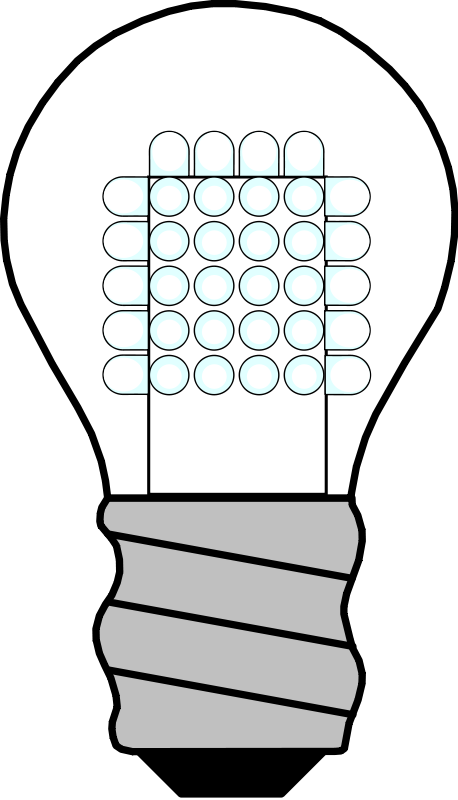
\includegraphics[scale=0.02]{imgs/bulb.png}
 \textbf{Nota} \\
 }%
{\endMakeFramed}

%Work in progress
\newenvironment{workinprogress}{%
  \def\FrameCommand{\colorbox{pink}}%
  \MakeFramed {\FrameRestore}
\lhdbend  \textbf{Work in progress} \\
 }%
{\endMakeFramed}

%Openquestion
\newenvironment{openquestion}{%
  \def\FrameCommand{\colorbox{pink}}%
  \MakeFramed {\FrameRestore}
 \textbf{Domanda aperta} \\
 }%
{\endMakeFramed}

%TODO
\newenvironment{todo}{%
  \def\FrameCommand{\colorbox{pink}}%
  \MakeFramed {\FrameRestore}
 \textbf{TODO} \\
 }%
{\endMakeFramed}

%%%%%%%%%%%%%%%%%%%%%%%%%%%%%%%%
%%%%%%%%%%%% HEADER %%%%%%%%%%%%
%%%%%%%%%%%%%%%%%%%%%%%%%%%%%%%%
\pagestyle{fancy}
% i comandi seguenti impediscono la scrittura in maiuscolo
% dei nomi dei capitoli e dei paragrafi nelle intestazioni
\renewcommand{\chaptermark}[1]{\markboth{#1}{}}
\renewcommand{\sectionmark}[1]{\markright{\thesection\ #1}}
\fancyhf{} % rimuove l'attuale contenuto dell'intestazione
% e del pi\`e di pagina
\fancyhead[LE,RO]{\bfseries\thepage}
\fancyhead[LO]{\bfseries\rightmark}
\fancyhead[RE]{\bfseries\leftmark}
\renewcommand{\headrulewidth}{0.5pt}
\renewcommand{\footrulewidth}{0pt}
\addtolength{\headheight}{0.5pt} % riserva spazio per la linea
\fancypagestyle{plain}{%
\fancyhead{} % ignora, nello stile plain, le intestazioni
\renewcommand{\headrulewidth}{0pt} % e la linea
}


%%%%%%%%%%%%%%%%%%%%%%%%%%%%%%%%
%%%%%%%%%%%% COLORS %%%%%%%%%%%%
%%%%%%%%%%%%%%%%%%%%%%%%%%%%%%%%
\definecolor{code}{gray}{0.3}


%%%%%%%%%%%%%%%%%%%%%%%%%%%%%%%%
%%%%%%%%%%%% NUMBERS %%%%%%%%%%%
%%%%%%%%%%%%%%%%%%%%%%%%%%%%%%%%
\setcounter{tocdepth}{3}
\setcounter{secnumdepth}{3}


%%%%%%%%%%%%%%%%%%%%%%%%%%%%%%%%
%%%%%%%%%%% DOC DATA %%%%%%%%%%%
%%%%%%%%%%%%%%%%%%%%%%%%%%%%%%%%
\title{Appunti di MNO}
\author{Gruppo Informatici Rampanti}
\date{ott 2010 - mag 2011}

\pdfinfo{%
  /Title    (Appunti di MNO)
  /Author   (Andrea Cimino e Lorenzo Muti)
  /Creator  (Andrea Cimino)
  /Producer (Lorenzo Muti)
  /Subject  (MNO)
  /Keywords (MNO)
}


%%%%%%%%%%%%%%%%%%%%%%%%%%%%%%%%
%%%%%%%%%%%%% UTILS %%%%%%%%%%%%
%%%%%%%%%%%%%%%%%%%%%%%%%%%%%%%%
% binary symbols
\newcommand{\modder}{\vdash _{R}}

% vertical gaps
\newcommand{\askip}{\vspace{0.5cm}}
\newcommand{\bskip}{\vspace{1.0cm}}

% various symbols
\newcommand{\qedhere}{\ensuremath{\Box}}
\newcommand{\qed}{\hfill \ensuremath{\Box}}

% substitution
\newcommand{\subst}[2]{^{#1} / _{#2}}

% denotational semantics function names
\newcommand{\bbracket}[1]{\left\llbracket #1 \right\rrbracket}

\newcommand{\aexpr}{\mathcal{A}}
\newcommand{\bexpr}{\mathcal{B}}
\newcommand{\cexpr}{\mathcal{C}}
\newcommand{\Aexpr}[1]{\mathcal{A} \bbracket{#1}}
\newcommand{\Bexpr}[1]{\mathcal{B} \bbracket{#1}}
\newcommand{\Cexpr}[1]{\mathcal{C} \bbracket{#1}}

\newcommand{\semdomset}[1]{(V_{#1})_{\bot}}

% semantic evaluations
\newcommand{\opereval}[3]{\left\langle #1, #2 \right\rangle \rightarrow #3}
\newcommand{\denaeval}[3]{\Aexpr{#1} #2 = #3}
\newcommand{\denbeval}[3]{\Bexpr{#1} #2 = #3}
\newcommand{\denceval}[3]{\Cexpr{#1} #2 = #3}

% rotated sqsubseteqs
\newcommand{\upsqsubseteq}{ $\begin{rotate}{90} $\sqsubseteq$ \end{rotate}$ }
\newcommand{\downsqsubseteq}{ $\begin{rotate}{270} $\sqsubseteq$ \end{rotate}$ }

% Space after paragraph declaration
\makeatletter
\renewcommand\paragraph{\@startsection{paragraph}{4}{\z@}%
  {-3.25ex\@plus -1ex \@minus -.2ex}%
  {1.5ex \@plus .2ex}%
  {\normalfont\normalsize\bfseries}}
\makeatother



% fast theorem and definition
\newcommand{\ftheo}[1]{\colorbox{YellowGreen}{#1}}
\newcommand{\fdefn}[1]{\colorbox{SkyBlue}{#1}}

\theoremstyle{break}
\theoremsymbol{\ensuremath{\clubsuit}}
\theoremseparator{\newline}
\newshadedtheorem{proc}[theo]{Procedura}

% bold math!
\newcommand{\bm}[1]{\mbox{\boldmath{$#1$}}}

\newcommand{\positive}[1]{\textbf{\color{green} +} #1}
\newcommand{\negative}[1]{\textbf{\color{red} -} #1}


\newtheoremlisttype{tab}%
{\begin{tabular*}{\linewidth}{@{}lrl@{\extracolsep{\fill}}r@{}}}%
{##1&##2&##3&##4\\}%
{\end{tabular*}}
\begin{document}
}
\providecommand{\outbpdocument}{\end{document}}
\else
\providecommand{\inbpdocument}{}
\providecommand{\outbpdocument}{}
\fi



\inbpdocument 

% 11 Marzo
\chapter{Il problema lineare dei minimi quadrati}

\section{Metodo delle equazioni normali}

Sia
\begin{equation}
  \label{eq:06minq01} Ax = b
\end{equation} 
un sistema lineare in cui la matrice $A \in \mathbb{C}^{m \times n}$ 
dei coefficienti \`e tale che $m \geq n$.  Se $m > n$, il sistema
(\ref{eq:06minq01}) ha pi\`u equazioni che incognite e si dice
sovradeterminato. Se il sistema (\ref{eq:06minq01}) non ha soluzione,
fissata una norma vettoriale $||\;.\;||$, si ricercano i vettori $x
\in \mathbb{C}^{n}$ che minimizzano la quantit\`a $||Ax − b||$.  In
norma 2, il problema diventa quello di determinare un vettore $x \in
\mathbb{C}^n$ tale che
 \begin{equation}
 \label{eq:06minq02} || Ax − b ||_{2} = \displaystyle \min_{y \in
\mathbb{C}^{n}} || Ay − b||_{2} = \gamma
 \end{equation} Tale problema viene detto problema dei minimi
quadrati.  Il seguente teorema caratterizza l'insieme $X$ dei vettori
$x \in \mathbb{C}^n$ che soddisfano alla (\ref{eq:06minq02}).

\begin{theo} Valgono le seguenti propriet\`a:
   \begin{enumerate}
   \item $x \in X$ se e solo se
     \begin{equation}
         \label{eq:06minq03} A^H Ax = A^Hb
     \end{equation} Il sistema (\ref{eq:06minq03}) viene detto sistema
delle equazioni normali o sistema normale.

\item $X$ \`e un insieme non vuoto, chiuso e convesso.

\item L'insieme $X$ si riduce ad un solo elemento $x^∗$ se e solo se
la matrice $A$ ha rango massimo.
\item Esiste $x^∗ \in X$ tale che
  \begin{equation}
\label{eq:06minq04} || x^{*}||_{2} = \displaystyle \min_{x \in X}
||x||_{2}
  \end{equation} Il vettore $x^{*}$ \`e l'unico vettore di $X$ che
appartiene a $N(A^{H}A)^{\bot}$ ed \`e detto \emph{soluzione di minima
norma}
   \end{enumerate}
\end{theo}

\begin{thproof}
  \begin{enumerate}
  \item Siano
$$ S(A) = \{ y \in \mathbb{C}^{m}: y = Ax 
\text{ per qualche } x \in \mathbb{C}^{m} \}$$ e
$$
S(A)^{\bot} = \{ z \in \mathbb{C}^{m} \; : \; z^{H}y = 0, \forall y
\in S(A) \}
$$
il sottospazio di $\mathbb{C}^m$ immagine di $A$, e il sottospazio
ortogonale a $S(A)$ (si vedano i paragrafi 2 e 6 del capitolo 1).  Il
%dio cane mettete i \ref!!!
vettore $b$ pu\`o essere cos\`i decomposto
 $$ b = b_1 + b_2, \quad \text{dove } 
 b_1 \in S(A) \text{ e } b_2 \in S(A)^{\bot} $$

per cui il residuo
$$ r=b_1 - Ax + b_2 = y + b_2, \quad
\text{dove } y=b_1 - Ax \in S(A) \text{ e } b_2 \in S(A)^{\bot}$$

vale
$$ ||r||_{2}^{2} = (y + b_2)^{H} (y + b_2) = 
||y||_{2}^{2} + ||b_2||_{2}^{2}$$ 

in quanto $y^{H}b_2 = b_2^{H}y=0$. Per minimizzare $||r||_{2}^{2}$,
non possiamo agire su $b_2$ poich\'e \`e costante, mentre possiamo
porre a zero $y$ che dipende da $x$, il che equivale a porre $b_1 = Ax$, 
che \`e verificato per qualche $x$ dato che $b_1$ appartiene al
sottospazio immagine di $A$. \\
A questo punto otteniamo 
$$ ||r||_{2}^{2} = ||b_2||_{2}^{2}$$

vero se e solo se il vettore $r$ appartiene a $S(A)^{\bot}$ ed \`e quindi ortogonale
alle colonne di $A$, cio\'e
$$A^{H}r = A^{H} (b − Ax) = 0$$
Ne segue quindi che $x \in X$ se e solo se $x$ \`e soluzione di
(\ref{eq:06minq03}).  Inoltre risulta $\gamma^{2} = ||b_2||_{2}^{2}$

Nel caso di $\mathbb{R}^2$ con una matrice $A$ di rango $1$ si pu\`o
dare la seguente interpretazione geometrica, illustrata nella figura
7.1. Il vettore $b = r − Ax$ risulta decomposto in un sol modo nel
vettore $b_2 = r \in S(A)^{\bot}$ e nel vettore $b_1 = Ax \in S(A)$.
Il vettore $Ax$ \`e quindi la proiezione ortogonale del vettore $b$
sul sottospazio generato dalle colonne di $A$.
\begin{todo} Inserire immaginina
\end{todo}

\item L'insieme $X$ non \`e vuoto dato che, per quanto detto
precedentemente, $Ax=b_1$ ha soluzione per come abbiamo scelto $b_1$.\\
% VERSIONE DELLE DISPENSE
% Se $x_0$ \`e tale che
% $$A^{H}Ax_0 = A^{H}b $$
% allora risulta
% $$ X = \{ x \in \mathbb{C}^{n} \; : \; x = x_0 + v, v
%  \in N(A^{H}A) \}$$ Quindi $X$ \`e una variet\`a lineare affine,
% parallela ad $N(A^{H} A)$, passante per $x_0$ , e poich\'e $N(A^{H}
% A)$ \`e chiuso e convesso, $X$ un insieme chiuso e convesso.\\

% VERSIONE FATTA A LEZIONE
Mostriamo ora che $X$ è chiuso e convesso:
\begin{enumerate}
\item caso $rank(A) = n$ \\ 
  $A^{H}A$ è definita positiva non singolare, $A^{H}Ax = A^{H}b$ ha
  soluzione unica ed $X$ è formato da un solo vettore.
\item caso $rank(A) < n$\\ 
  $A^{H}A$ è semi-definita positiva, $det(A^H A) = 0$,
  abbiamo infinite soluzioni delle forma
  $$X = \{ x = x_0 + v\} \qquad v \in Ker(A^{H}A)$$
  e poich\'e $N(A^{H} A)$ \`e chiuso e convesso, $X$ un insieme chiuso
  e convesso.\\

  Ad esempio poniamo che il rango sia 1 in $\mathbb{R}^2$ con $n =2$,
  allora $dim(Ker(A^{H}A)) = 1$ e $rank(A^{H}A) = 1$, l'insieme delle
  soluzioni $X$ è una retta, che è un insieme chiuso e convesso.
\end{enumerate}

\item per quanto detto al secondo punto se $A$ ha rango massimo, $X$
  contiene un solo elemento. In tal caso l'insieme $N (A^{H} A)$ \`e 
  costituito dal solo elemento nullo.

\item l'esistenza della soluzione di minima norma \`e ovvia
  nel caso in cui $X$ si riduce al solo elemento $x$.\\
  Invece se $A$ non ha rango massimo, per quanto detto al secondo punto, $X$
  è formato da infiniti elementi ed esiste $x^{*} \in X$ tale che
  $||x^{*}|| = \min_{X} ||x||$ e $x^{*}$ è l'\emph{unica} soluzione
  appartenente a $Ker(A^H A)^{\bot}$.\\

  Versione più approfondita dalle dispense:\\
  Se $X$ non si riduce al solo elemento $x^{∗}$ , sia $x_0 \in X$ e si consideri
  l’insieme
  $$ B = \{ x \in \mathbb{C}^{n}\; : \; ||x||_{2} \leq ||x_0||_2 \}$$
  Poich\'e, se $x \in X$, ma $x \notin B$, risulta $||x||_{2} >
  ||x_0||_{2}$, allora
  $$  \displaystyle 
  \min_{x \in X} ||x||_{2} = \min_{x \in X \cap B} ||x||_{2}
  $$
  L'insieme $X \cap B$ \`e un insieme non vuoto, limitato e chiuso, in
  quanto intersezione di insiemi chiusi, e quindi compatto; essendo la
  norma una funzione continua, esiste un $x^∗ \in X \cap B$ per cui vale
  la (\ref{eq:06minq04}).

  Inoltre $x^*$ \`e l'unico vettore di $X$ appartenente a a
  $N(A^{H}A)^{\bot}$ Infatti esistono e sono unici $ y \in N (A^{H} A)$
  e $z \in N (A^{H} A)^{\bot}$ tali che $x^{∗} = y + z$ Poich\'e $x^*$
  \`e soluzione di (\ref{eq:06minq03}).  $ A^{H} A(y + z) = A^H b$, da
  cui $A^H Az = A^H b$ e quindi z \`e soluzione del problema
  (\ref{eq:06minq02}).  Se $y$ non fosse uguale a 0, $z$ avrebbe norma 2
  minore di $||x^*||$ , ci\`o \`e assurdo perch\'e $x^∗$ \`e la
  soluzione di minima norma: ne segue che $x^* = z \in N (A^H A)^{\bot}$.

  Nel caso di $\mathbb{R}^2$ con una matrice $A$ di rango 1, si pu\'o
  dare l’interpretazione geometrica illustrata nella figura in cui \`e
  riportata la variet\`a $X$, parallela alla variet\`a $N (A^H A)$.  Il
  punto $x_0$ un qualunque punto di $X$. Il punto $x^∗$ \`e quello di
  minima norma e quindi quello pi\`u vicino all’origine $O$ dello spazio
  $\mathbb{C}$
\end{enumerate}
\end{thproof}

\paragraph{Risoluzione tramite Cholesky} 
Se la matrice A ha rango massimo, allora la soluzione del problema dei
minimi quadrati pu\`o essere ottenuta risolvendo il sistema
$$A^{H}Ax = A^{H}b$$
In tal caso, poich\'e la matrice $A^{H}{A}$ \`e definita positiva
(\ref{prop:def-pos}), si pu\`o utilizzare per la risoluzione il metodo
di Cholesky \ref{sec:fatt-cholesky}.
Determinata la matrice triangolare inferiore tale che
$$LL^{H} =A^{H} A$$
la soluzione $x^{*}$ di $A^{H}Ax = A^{H}b$ viene calcolata risolvendo
successivamente i due sistemi di ordine $n$ con matrice di
coefficienti triangolare
$$Ly = A^H b$$
$$L^H x = y$$

Se la matrice $A$ non ha rango massimo, non si pu\`o risolvere il 
sistema 
(\ref{eq:06minq03}) con il metodo di Cholesky, ma si pu\`o
 applicare il metodo di Gauss con la variante del massimo pivot.

\paragraph{Costo}
Nel caso di una soluzione:
\begin{itemize}
\item Calcolo di $A^{H}A$ :$ n^{2}m/2$ per la costruzione della
matrice hermitiana
\item Cholesky: $n^{3}/6$ per la risoluzione del sistema
\end{itemize} In totale quindi il costo \`e: $n^{2}((m/2) + (n/6))$

\begin{workinprogress} 
Condizionamento, definito solo per le quadrate,
per le rettangolari si passa per SVD,
$$ \mu(A) = ||A|| ||A^{-1}||$$
$$  \mu(A^{H}A) = \mu^{2}(A)$$
Cholesky è stabile
\end{workinprogress}

\section{Metodo QR} 
Si esamina ora un altro procedimento, detto metodo QR, che opera
direttamente sulla matrice A fattorizzandola nella forma QR
\ref{fatt:QR}, dove $Q$ \`e una matrice ortogonale.  In particolare,
poich\'e si sta lavorando nel campo complesso, $Q$ \`e unitaria. \\
Si supponga dapprima che la matrice $A \in C^{m\times n} $ abbia rango
massimo, $k = n \leq m$.  Si applica il metodo di Householder alla
matrice $A$, ottenendo una successione di matrici di Householder 
\ref{sec:householder}.
$$ P^{(k)} \in \mathbb{C}^{m \times m }, k =1, \ldots, n$$
Posto $Q^{H} = P^{(1)} P^{(2)}\ldots P^{(n)}$ risulta
\begin{equation}
  \label{eq:06minq05} A=QR
\end{equation} 
dove la matrice $R \in \mathbb{C}^{m \times n}$ ha la forma

\begin{equation}
  \label{eq:06minq06} R = \left[
\begin{array}{l} R_1 \\ \\ 0
\end{array} \right]
\begin{array}{l} \}n \text{ righe} \\ \\ \}m-n \text{ righe}
\end{array}
\end{equation}

ed $R_1$ \`e una matrice triangolare superiore non singolare in quanto
$A$ ha rango massimo. Dalla (\ref{eq:06minq05}) si ha

\begin{equation}
  \label{eq:06minq07} 
  || Ax - b ||_2 = ||QRx - b||_2 \underbracket{=}_{*)} 
  ||QRx - QQ^{H}b||_2 = ||Q(Rx - Q^{H}b)||_2 = ||Rx - Q^{H}b||_2 = 
  ||Rx - c||_2
\end{equation}
*) Le matrici unitarie preservano la norma 2 (\ref{prop:unitarie})\\

dove $c = Q^H b$. Partizionando il vettore $c$ nel modo seguente
$$
  c = \left[
\begin{array}{l} c_1 \\ \\ c_2
\end{array} \right]
\begin{array}{l} \}n \text{ componenti} \\ \\ \}m-n \text{ componenti}
\end{array}
$$
per la (\ref{eq:06minq06}) vale
$$
Rx - c = \left[
\begin{array}{c} R_1 x -c_1 \\ -c_2
\end{array} \right]
$$
per la (\ref{eq:06minq07}) risulta
$$\min_{x \in \mathbb{C}^{n}}||Ax-b ||_{2}^{2}
= \min_{x \in \mathbb{C}^{n}}||Rx-c ||_{2}^{2} = \min_{x \in
\mathbb{C}^{n}}[||R_1x-c_1 ||_{2}^{2} + ||c_2||_2^2] = ||c_2||_2^2 +
\min_{x \in \mathbb{C}^{n}} ||R_1x - c_1 ||_{2}^{2}
 $$
Poich\'e $R_1$ \`e non singolare, la soluzione $x^{*}$ del sistema
lineare
\begin{equation}
 \label{eq:06minq08} R_1x = c_1
\end{equation} \`e tale che
$$
\min_{x \in \mathbb{C}^{n}} ||R_1 x - c_1||_2 = ||R_1 x^{*} -c_1||_2 =
0
$$
ne segue che $x^*$ \`e la soluzione del problema
$$|| Ax − b ||_{2} = \displaystyle \min_{y \in
\mathbb{C}^{n}} || Ay − b||_{2} = \gamma$$ e si ottiene
$$\gamma = ||c_2||_2$$

\begin{notes} Mi sembra che la parte parte sull'evitare il calcolo
delle matrici $P^{(k)}$ e $Q$ non l'ha spiegata, ma la scrivo per
completezza.
\end{notes} Analogamente al caso della risoluzione dei sistemi
lineari, il metodo pu\`o essere applicato senza calcolare
effettivamente n\'e le matrici $P^{(k)}, k =1\ldots n$, n\'e la
matrice $Q$.  Si pu\`o procedere infatti nel modo seguente: sia
$$P^{(k)} = I - \beta_{k} v_k v_k^{H}, \quad
k=1, \ldots n$$ Consideriamo la matrice
$$T^{(1)} = [A \; | \; b]$$
e si costruisce le successioni delle matrici $T^{(k)}$ tali che
$$
T^{(k+1)} = P^{(k)}T^{(k)} = T^{(k)} - \beta_k v_k v_k^{H} T^{(k)}
$$
Al termine dopo $n$ passi si ottiene la matrice
$$ T^{(n+1)} = [R \; | \; c ] $$

\subsection{Casi e Costi} \subparagraph{Rango massimo} Nel caso
$det(R_1) \neq 0 \; \Longleftrightarrow \; rank(A) =n$, abbiamo
un'unica soluzione. La complessit\`a computazionale \`e data da:
\begin{itemize}
 \item Calcolo $QR$: $n^{2}(m-n/3) \approx n^{2}m$ (circa il doppio di
Cholesky)
\item Risolvere $x = R_1^{-1} C_1$: $n^2$ operazioni
\end{itemize} In generale quindi $QR$ richiede pi\`u operazioni, ma se
$m=n$ i due metodi hanno lo stesso costo.

\subparagraph{Rango $<n$: metodo del massimo pivot} 
In questo caso esistono infinite soluzioni, ed \`e necessario
provvedere ad una riformulazione del problema nel seguente modo
$$ A\Pi = QR$$ 
dove $\Pi$ \`e una matrice di permutazione delle colonne.  Infatti se
la matrice $A$ non ha rango massimo, la matrice $R_1$ ottenuta ha
almeno un elemento diagonale nullo e quindi non \`e possibile
calcolare la soluzione del sistema (\ref{{eq:06minq08}}). \\
Questa difficolt\`a viene superata applicando il metodo QR con la
tecnica \emph{del massimo pivot} (\ref{qr-max-pivot})per colonne nel
modo seguente: al $k$-esimo passo, costruita la matrice $A^{(k)}$
della forma
$$
A^{(k)} = \left[
  \begin{array}{lll} 
    C^{(k)} &  & D^{(k)}                                  \\ 
            &  &                                          \\ 0 &  & B^{(k)}
  \end{array} 
\right]
\begin{array}{l} 
  \} k-1 \text{ righe}                                    \\ 
                                                          \\ 
  \}m-k+1 \text{ righe}
\end{array}
$$

si determina la colonna di $B^{(k)}$ la cui norma 2 \`e massima. Sia
$j, 1 \leq j \leq n-k+1$ l'indice di tale colonna. Se $j = 1$, si
scambiano fra loro la $k$-esima e la $(k + j − 1)$-esima colonna della
matrice $A^{(k)}$ . Quindi si applica la matrice elementare $P^{(k)}$
alla matrice con le colonne cos\`i permutate.  Se il rango di A \`e $r
< m$, questo procedimento termina dopo $r$ passi, e si ottiene una
decomposizione del tipo
$$ A\Pi = QR$$ 
dove $\Pi \in \mathbb{R}^{n \times n}$ \`e una matrice di
permutazione, $Q \in \mathbb{C}^{m \times m}$ \`e una matrice unitaria
ed $R$ \`e della forma
$$
 A^{(k)} = \left[
\begin{array}{lll} R_1 & & S \\ & & \\ O & & O
\end{array} \right]
\begin{array}{l} \} r \text{ righe} \\ \\ \}m-r \text{ righe}
\end{array}
$$
in cui $R_1 \in C^{r \times r}$ \`e triangolare superiore non
singolare e $S \in \mathbb{C}^{r \times (n -r)}$. Gli elementi
diagonali di $R_1$ risultano positivi ed ordinati in ordine modulo non
crescente .
\begin{notes} Il professore su questo ultimo punto \`e stato vago, ma
sul libro \`e spiegato tutto per bene.
\end{notes}

\begin{workinprogress} \textbf{Cosa avra mai voluto dire?} \\ Costo:
$(m-k) (n-k) + (m-k)(n-k)$ \\ Sommando su tutti i $k$
$$
\displaystyle 2 \sum_{k=1}^{n} (m-k)(n-k)
$$
$$i =n-k \quad i =1, \ldots, n \quad k = n-i$$
$$ 
2 \displaystyle \sum_{i=1}^{n} (m-n+i)i = 2 (\displaystyle
\sum_{i=1}^{n} (m-n) i + \displaystyle i^{2}) = 2 (( m-n)
\frac{n^{2}}{2} + \frac{n^3}{3}) = (m-n)n^{2} + \frac{2}{3}n^{3}
$$   
\end{workinprogress}

\section{Norme di matrici non quadrate} Per comprendere i successivi
metodi, \`e necessario introdurre questo concetto.  Sia $A \in
\mathbb{C}^{m\times n}$. Le norme matriciali indotte, come gi\`a visto
in precedenza, vengono definite per mezzo della relazione
$$ || A|| = \max_{||x||' = 1} ||Ax ||'' = \sup_{x \neq 0}
\frac{||Ax||}{||x||}
$$
dove $|| \; . \; ||$ e $|| \; . \; ||''$ sono norme vettoriali
rispettivamente su $\mathbb{C}^{n}$ e $\mathbb{C}^{m}$. \\ Estendiamo
questo concetto sulla matrici $m \times n$, usando la norma 2,
usandola in $|| \; . \; ||$ e $|| \; . \; ||''$.  Si dimostra che:
$$ || A||_{2} = \sqrt{\rho(A^{H}A)}
\qquad \text{($\rho$: raggio spettrale)}
$$
Utilizzando invece la norma, di Frobenius otteniamo
$$ ||A||_{F} = \sqrt{tr(A^{H}A)} =
\sqrt{\displaystyle \sum_{i,j}|a_{ij}|^{2} } \qquad \text{(tr =
traccia)}
$$ 
Questa non è una norma indotta.

\paragraph{Invarianza della norme} Se $U \in \mathbb{C}^{m \times m}$
e $V \in \mathbb{C}^{n\times n}$ sono matrici unitarie, poiché
$$ (U^{H}AV)^{H}(U^{H}AV) = V^{H}A^{H}AV$$
risulta
$$|| U^{H}AV||_{2} = \sqrt{\rho(A^{H}A)} = ||A||_{2}$$
La stessa cosa vale per la norma di Frobenius. \\ \\ A lezione
Bevilacqua ha scritto:
$$ || AU||_{2}^{2} = \rho (U^{H} A^{H}A U)
= \rho(A^{H}A) = ||A||_{2}^{2}
$$
$$ ||UA ||_{2}^{2} = \rho(A^{H} U^{H}UA)
= \rho(A^{H}A) = ||A||_{2}^{2}$$

\section{SVD: Decomposizione ai valori singolari di una matrice }
Vedremo un metodo per risolvere il problema dei minimi quadrati,
tramite un nuovo tipo di fattorizzazione: la SVD.  Il pregio di questo
metodo \`e che vengono coinvolte matrici unitarie che hanno garanzie di
stabilità. \\ 
Assomiglia ad una trasformazione per similitudine ma non lo \`e.

% TODO
% Ricordiamo che se $A$ \`e hermitiana e semidefinita positiva, allora
% ci siamo riportati al metodo
% $$ A = QDQ^{H} \qquad D = diag(\lambda_i)$$
% $\lambda_i$ autovalori, colonne di Q sono gli autovettori. \\

\begin{theo} Sia $A \in \mathbb{C}^{m \times n}$. Allora esistono una matrice
unitaria $U \in \mathbb{C}^{m \times m}$ ed una matrice unitaria $V
\in \mathbb{C}^{n \times n}$ tali che
\begin{equation}
  \label{eq:06minq09} A = U \Sigma V^{H}
\end{equation} dove la matrice $\Sigma \in \mathbb{R}^{m \times n}$ ha
elementi $\sigma_{ij}$ nulli per $i \neq j$ e per $i =j$ ha elementi
$\sigma_{ii} = \sigma_i$ con
$$
\sigma_1 \geq \sigma_2 \geq \ldots \sigma_p \geq 0, \quad p =
\min\{m,n\}
$$
La decomposizione \`e detta decomposizione ai valori singolari della
matrice $A$, mentre i valori $\sigma_i$, per $i = 1, \ldots , p,$ sono
detti \textbf{valori singolari} di $A$. Indicate con $u_i , i = 1,
\ldots , m,$ e $v_i , i = 1, \ldots , n$, le colonne rispettivamente
di $ U$ e di$ V$ , i vettori $u_i$ e $v_i$ , $i = 1, \ldots , p,$ sono
detti rispettivamente \textbf{vettori singolari sinistri} e
\textbf{vettori singolari destri} di $A$.  La matrice $\Sigma$ \`e
univocamente determinata, anche se le matrici $U$ e $V$ non lo sono.
\end{theo}

\begin{figure}[hb] \centering
$$
\Sigma =
\begin{pmatrix} 
  \sigma_1 & 0        & 0      & 0      & 0        \\ 
  0        & \sigma_2 & 0      & 0      & 0        \\
  0        & 0        & \ddots & 0      & 0        \\ 
  0        & 0        & 0      & \ddots & 0        \\ 
  0        & 0        & 0      & 0      & \sigma_n \\
\end{pmatrix} $$

$$ \sigma_i \in \mathbb{C}
\quad \sigma_1 \geq \sigma_2 \geq \ldots \geq \sigma_n \geq 0$$
\caption[Struttura della matrice $\Sigma$]{Struttura della matrice
  $\Sigma$}
\end{figure}

\begin{thproof} Si considera per semplicit\`a il caso $m \geq n$ (se
$m < n$, si sostituisce $A$ con $A^H$). Si procede dimostrando per
induzione su $n$ che la tesi vale per ogni $m \geq n$.  Per $n = 1$
\`e $A = a \in \mathbb{C}^m$.  Si pone $\sigma_1 = ||a||_2$ e si
considera come matrice $U$ la matrice di Householder tale che $Ua =
\sigma_1e_1$. La matrice $V$ \`e la matrice $V = [1]$.  \\ Per n > 1
si dimostra che se la tesi vale per le matrici di $C^{k \times
(n-1)}$, con $k \geq n-1$¸ allora vale per le matrici di $C^{k \times
(n)}$ con $m \geq n$ . Sia $ x \in \mathbb{C}^{n}$ tale che $||x||_2 =
1 $ e $||A||_2 = ||Ax||_2$.  Si consideri il vettore
 $$y = \dfrac{Ax}{||Ax||_2} \in \mathbb{C}^{n}$$

Allora $||y||_2 = 1$ e $Ax = \sigma_1y,$ con $\sigma_1 =
||A||_2$. Siano poi $V_1 \in \mathbb{C}^{n \times n} $ e $U_1 \in C^{m
\times m}$ matrici unitarie le cui prime colonne sono uguali
rispettivamente a $x$ e $y$. Poich\'e
$$U_1^{H} AV_1e_1 = U_1^H Ax 
= U_1^{H} \sigma_1 y = \sigma_1[1; 0; \ldots ; 0]^T $$ \`e
\begin{notes}
Quest'ultimo passaggio si spiega col fatto
che $U_1$ \`e unitaria, allora anche la sua trasposta
coniugata \`e unitaria, allora $U^{h} U = I$, Se al posto
di $U$ prendiamo proprio $y$, ottieniamo la prima colonna
della matrice identit\`a
\end{notes}

$$
 A_1 = U_1^{H}AV_1 = \left[
\begin{array}{lll} \sigma_1 & & w^{H} \\ & & \\ 0 & & B
\end{array} \right]
\begin{array}{l} \}1 \text{ riga} \\ \\ \}m-1 \text{ righe}
\end{array}
$$
in cui $w \in \mathbb{C}^{n−1}, B \in \mathbb{C}^{(m−1)\times(n−1) }$
e $\mathbf{0} \in \mathbb{C}^{m−1}$.  Si dimostra ora che $w = 0$. Si
supponga per assurdo ch e $w \neq 0$ e si consideri il vettore $z =
\left[
 \begin{array}{l} \sigma_1 \\ w
\end{array} \right] \neq \mathbf{0} $ per cui
$$
A_1z = \left[
  \begin{array}{c} \sigma_1^{2} + w^{H}w \\ Bw
  \end{array} \right]
$$
 Si ha

$$
||A_1 z||_2^2 = ||z||_2^4 + || Bw||_2^{2} \geq ||z||_2^4
$$
da cui, dividendo per $||z||_2^2$ si ottiene
$$
\dfrac{||A_1z||_2^2}{||z||_2^2} \geq ||z||_2^2
$$
e quindi
\begin{equation}
  \label{eq:06minq10} ||A_1||_2^{2} \geq \sigma_1^{2} + w^{H}w.
\end{equation}
D'altra parte \`e $||A_1||_2 = ||A||_2$ 
 in quanto $A_1$ \`e ottenuta da $A$ con trasformazioni unitarie e
quindi
 \begin{equation}
   \label{eq:06minq11} ||A_2||_2 =\sigma_1.
 \end{equation} Dal confronto fra la (\ref{eq:06minq10}) e la
(\ref{eq:06minq11}) segue l’assurdo. Quindi

$$
A_1 \left[
\begin{array}{ccc} \sigma_1 & & \mathbf{0}^{H}\\ & & \\ \mathbf{0} & &
B \\
\end{array} \right]
$$
Dalla (\ref{eq:06minq11}) segue che
\begin{equation}
  \label{eq:06minq12} \sigma_1 \geq ||B||_2
\end{equation} Infatti
$$
\sigma_1^{2} = ||A_1||_2^{2} =  \rho(A_1^{H}A_1) = \rho \left( \left[
\begin{array}{ccc} \sigma_1^2 & & \mathbf{0}^{H}\\ & & \\ \mathbf{0} &
& B^{H}B
\end{array} \right] \right) = \max [\sigma_1^{2}, \rho(B^{H}B)] \geq
\rho (B^H B) = ||B||_2^2 .
$$
Poich\'e $B \in C^{(m−1)\times(n−1)} $e $m − 1 \geq n − 1$, per
l'ipotesi induttiva si ha
$$
U_2^{H}BV_2 = \Sigma_2
$$
dove le matrici $U_2 \in \mathbb{C}^{(m−1)\times(m−1)}$ e $V_2 \in
\mathbb{C}^{(n−1)\times(n−1)}$ sono unitarie e $\Sigma_2 \in
\mathbb{R}^{(m−1)\times(n−1)}$ ha elementi $\sigma_2 \geq \ldots \geq
\sigma_p$ . Poich\'e $\sigma_2 = ||B_2|| \leq \sigma_1$ per la
(\ref{eq:06minq12}), la tesi segue con
$$
U= U_1 \left[
\begin{array}{ccc} 1 & & \mathbf{0}^{H}\\ & & \\ \mathbf{0} & & U_2
\end{array} \right], \; V = V_1 \left[
\begin{array}{ccc} 1 & & \mathbf{0}^{H}\\ & & \\ \mathbf{0} & & V_2
\end{array} \right], \; \Sigma = \left[
\begin{array}{ccc} \sigma_1 & & \mathbf{0}^{H}\\ & & \\ \mathbf{0} & &
\Sigma_2
\end{array} \right]
$$

Le matrici $U$ e $V$ non sono univocamente determinate: infatti se
$$ A = U \Sigma V^{H}$$
\`e una decomposizione ai valori singolari di $A$, e se $S \in
\mathbb{C}^{n \times n}$ una matrice di fase e $Z \in
\mathbb{C}^{(m-n) \times (m-n)}$ \`e una matrice unitaria, anche

$$
A = U \left[
\begin{array}{ccc} S & & 0\\ & & \\ 0 & & Z
\end{array} \right] \Sigma S^{H}V^{H}
$$
\`e una decomposizione ai valori singolari di $A$.  Inoltre se
$\sigma_i = \sigma_{i+1} = \ldots = \ \sigma_{i+j}$ , per $j \geq 1$,
detta $P$ una qualunque matrice unitaria di ordine $j + 1$ e
considerata la matrice diagonale a blocchi
$$
Q= \left[
\begin{array}{ccc} I_{i-1} & O & O \\ & & \\ O & P & O \\ & & \\ O & O
& I_{n-j-i} \\
\end{array} \right]
$$
si ha che

$$
A= U \left[
\begin{array}{cc} Q & O \\ & \\ O & I_{m-n}
\end{array} \right] \Sigma Q^{H}V^{H}
$$
\`e una decomposizione ai valori singolari di $A$
\end{thproof} Dal teorema segue che
\begin{equation}
  \label{eq:06minq13} A = U\Sigma V^{H} = \displaystyle \sum_{i=1}^{p}
\sigma_i u_i v_i^{H}
\end{equation}

$$
\left.
\begin{array}{c} Av_i = \sigma_i u_i \\ A^{H} u_i = \sigma_i v_i
\end{array} \right\}, i=1,\ldots, p
$$
\begin{workinprogress}
\paragraph{Costi}
\begin{itemize}
 \item  Diagonalizzazione: $A^{H}A$ : $\frac{1}{2}mn^{2}$
 \item $A^{H}A$: $O(n^{3})$
 \item  Fattorizzazione $QR$, costo : $mn^{2}$
\end{itemize}
Normalmente costa $\frac{1}{2} mn^{2}$, usando Golum costa $2mn^{2}$
ma \`e più stabile. (Ricontrollare tutto)  
\end{workinprogress}

\begin{theo}
 % 7.10
\label{eq:06minq33}
 Sia $A \in \mathbb{C}^{m \times n}$ e sia
$$A = U\Sigma V^{H}$$
la sua decomposizione ai valori singolari, dove
$$\sigma_1 \geq \sigma_2 \geq . . .
 \geq \sigma_k > \sigma_{k+1} = \ldots = \sigma_p = 0.
$$
Allora valgono le seguenti propriet\`a
\begin{enumerate}
\item
$$ A = U_k \Sigma_k V_k^{H}
= \displaystyle \sum_{i=1}^{k} \sigma_i u_i v_i^{H} , \quad \text{
dove}
$$
$U_k \in \mathbb{C}^{m\times k}$ \`e la matrice le cui colonne sono
$u_1 , \ldots , u_k$ , \\ $V_k \in \mathbb{C}^{n×k}$ \`e la matrice le
cui colonne sono $v_1 , \ldots, v_k$ , \\ $\Sigma_k \in
\mathbb{R}^{k\times k}$ \`e la matrice diagonale i cui elementi
principali sono
$$ \sigma_1, \ldots \sigma_k$$

\item Il nucleo di $A$ \`e generato dai vettori $v_{k+1} ,\ldots ,
v_n$ .

\item L'immagine di $A$ \`e generata dai vettori $u_1, \ldots , u_k$,
e quindi
$$rank(A) = k$$
\item

 $\sigma_i^{2} , i = 1, \ldots, p$ sono gli autovalori della matrice
$A^H A$ (se $m < n$ i restanti autovalori sono nulli) e quindi
$$
||A||_{F}^{2} = \displaystyle \sum_{i=1}^{k} \sigma_i^{2}
$$
$$||A||_2 = \sigma_1 $$

\item Se $m = n$ e $A$ \`e normale, allora $\sigma_ii = |\lambda_i |,
i = 1, \ldots , n$, dove i $\lambda_i$ sono gli autovalori di $A$, e i
vettori singolari destri e sinistri coincidono con gli autovettori di
$A$.
\end{enumerate}

\end{theo}

\begin{thproof} 
Si supponga per semplicit\`a che $p = n \leq m$ (se $n
> m$ si sostituisce $A$ a con $A^{H}$ ).
\begin{enumerate}
\item La matrice $\Sigma$ ha la forma
$$
\left[
\begin{array}{lll} \Sigma_{k} & & O \\ & & \\ O & & O
\end{array} \right]
\begin{array}{l} \} k \text{ righe} \\ \\ \}m-k \text{ righe}
\end{array}
$$
per cui, partizionando le matrici $U$ e $V$ nel modo seguente
$$U = [U_k | U'_{m−k} ] \qquad V = [V_k | V_{n−k} ]$$
Dalla (\ref{eq:06minq13}) risulta che
\begin{equation}
  \label{eq:06minq14} A = U_k \Sigma_k V_k^{H}
\end{equation}

\item Se $x \in \mathbb{C}^n$ , la condizione $Ax = 0$ per la
(\ref{eq:06minq13}) equivalente alla condizione
$$U \Sigma V^{H} x = 0$$
e, poich\'e U non singolare, ` equivalente a
\begin{equation}
  \label{eq:06minq15} \Sigma V^H x = 0
\end{equation} Il vettore $z = \Sigma V^H x$ pu\`o essere partizionato
nel modo seguente

\begin{equation}
  \label{eq:06minq16} \left[
\begin{array}{l} \Sigma_{k}V_k^{H}x \\ \\ O
\end{array} \right]
\begin{array}{l} \} k \text{ compomenti} \\ \\ \}m-k \text{
componenti}
\end{array}
\end{equation}

per cui la (\ref{eq:06minq15}) pu\`o essere scritta come $\Sigma_k
V_k^{H} x = 0$, ossia $V_k^{H} x = 0$.  Quindi $Ax = 0$ se e solo se
$x$ \`e ortogonale alle prime $k$ colonne di $V$ ed essendo $V$
unitaria, se e solo se $x$ \`e generato dalle restanti colonne e di V
.

\item Dalla (\ref{eq:06minq14}) risulta che
\begin{equation}
  \label{eq:06minq17} y=Ax = U_k \Sigma_k V_k^{H}x = U_kz
\end{equation} dove $z = \Sigma_k V_k^{H}x \in \mathbb{C}^{k}$. Quindi
$y$ \`e generato dalle colonne di $U_k$. Viceversa (20) si ha che,
poich\'e la matrice $\Sigma_kV_k$ \`e di rango massimo, per ogni $x
\in \mathbb{C}^{n} , x \neq 0, $ esiste uno $z \neq 0$ per cui vale la
(21).

\item Dalla (\ref{eq:06minq13}) si ha che
$$A^H A = V\Sigma^H \Sigma V^H$$
dove $\Sigma^{H}\Sigma \in \mathbb{R}^{n\times n}$ \`e la matrice
diagonale i cui elementi principali sono 
$\sigma_1^{2},\ldots, \sigma_p^{2}$. Poich\'e la traccia e il raggio
spettrale di due matrici simili sono uguali, si ha
$$
||A||_F^{2} = tr(A^{H}A) = \displaystyle \sum_{i=1}^{p} \sigma_i^{2} =
\sum_{i=1}^{k} \sigma_i^{2}
$$
e
$$
||A||_{2}^{2} = \rho(A^{H}A) = \sigma_1^{2}
$$
e poich\'e $\sigma_1 > 0$ risulta $||A||_2 = \sigma_1$

\item Se $A$ \`e normale, dalla forma normale di Schur di $A$

$$A = U DU^{H}$$ ,
segue che
$$A^H A = UD^{H} DU^H$$
perci\`o gli autovalori $\sigma_i$ di $A^H A$ sono tali che

$$\sigma_i^{2} = \overline{\lambda}_i \lambda_i = |\lambda_i |^2
\quad \text{ per } i = 1, \ldots,n
$$

\end{enumerate}
 
\end{thproof}

\subsection{Calcolo dei valori e vettori singolari}

Dal teorema (\ref{eq:06minq10}) 
si pu\`o ricavare anche un procedimento per calcolare
i valori e i vettori singolari di $A$. Per semplicit\`a si suppone
 $m \geq  n$ (se fosse  $m < n$ basta riferirsi alla matrice
 $A^H$ ). Questo procedimento si articola nei seguenti passi:
 \begin{enumerate}
 \item   si calcolano gli autovalori e gli autovettori,
 normalizzati in norma 2, della matrice $A^H A$ e si considera la
 seguente decomposizione in forma normale di Schur della matrice
$ A^H A$
\begin{equation}
  \label{eq:06minq18}
A^H A = QDQ^H , D \in \mathbb{R}^{n\times n} , Q \in 
\mathbb{C}^{n \times n}   
\end{equation}
in cui gli elementi principali di $D$ sono gli autovalori in 
ordine non crescente di $A^H A$ e $Q$ \`e la corrispondente 
matrice degli autovettori ($Q$ \`e unitaria) (un
metodo stabile per calcolare la decomposizione 
(\ref{eq:06minq18}) sar\`a
 descritto nel  paragrafo 9);

\item
 si calcola la matrice
 \begin{equation}
   \label{eq:06minq19}
  C = AQ \in \mathbb{C}^{m \times n} 
 \end{equation}
e si determina, utilizzando la tecnica del massimo pivot 
per colonne, la fattorizzazione $QR$ della matrice
\begin{equation}
  \label{eq:06minq20}
  C\Pi  = UR = U 
\left[
\begin{array}{c}
R_1  \\
     \\
O
\end{array}
\right]
\end{equation}
dove $\Pi \in \mathbb{R}^{n \times n}$ \`e una matrice di
permutazione, $U \in C^{m \times m}$ \`e una matrice unitaria ed $R_1
\in \mathbb{C}^{m \times m}$ \`e una matrice triangolare superiore con
gli elementi principali reali non negativi e ordinati in modo non
crescente. Le condizioni imposte sull'ordinamento degli elementi
principali di $R_1$ rendono unica questa fattorizzazione se gli
elementi principali di $R_1$ sono tutti distinti.

 \end{enumerate}
Da (\ref{eq:06minq19}) e 
(\ref{eq:06minq20}) si ottiene,
ricordando che $Q^{-1} = Q^{H}$, $C\Pi = UR \;\rightarrow \; C = UR\Pi^{T}$
\begin{equation}
  \label{eq:06minq21}
A = U R\Pi^T Q^H ,
\end{equation}
da cui
$$A^H A = Q\Pi R^H U^H U R\Pi^T Q^H = Q\Pi R^H R\Pi^T Q^H =
 Q\Pi R_1^{H} R_1 \Pi^{T}Q^{H}$$

e quindi per la  (\ref{eq:06minq18}) risulta

$$R_1^{H} R_1 = \Pi^T D\Pi$$

Poich\'e la matrice $\Pi^T D\Pi$ risulta essere diagonale, ne segue che $R_1^{H} R_1$ 
\`e  diagonale, e quindi $R_1$ non pu\`o che essere diagonale.
 Inoltre, poich\`e gli  
 elementi principali di $R_1$ e di $D$ sono ordinati in modo non 
crescente, se gli  autovalori di $A^H A$ sono tutti distinti 
$ \Pi = I$. Quindi la (\ref{eq:06minq21}), se si pone
$ \Sigma = R$ e $V = Q\Pi$, rappresenta la decomposizione ai valori
 singolari di $A$.

\section{Risoluzione del problema dei minimi quadrati con i valori singolari}
Utilizzando il teorema \label{eq:06minq33} \`e possibile dare una
formulazione esplicita e della soluzione $x^*$ di minima norma del
problema dei minimi quadrati e del corrispondente $\gamma$, anche nel
caso in cui la matrice $A$ non sia di rango massimo.

\begin{theo}
 Sia $A \in  \mathbb{C}^{m \times n}$
 di rango $k$, con $m \geq n \geq k$, e sia
$$A = U \Sigma V^H$$
la decomposizione ai valori singolari di $A$. 
Allora la soluzione di minima norma del problema (2) \`e data da
$$
x^{*} = \displaystyle \sum_{i=1}^{k}
\dfrac{u_i^{H}b}{\sigma_i}v_i
$$
e
$$
\gamma^2 = \displaystyle \sum_{i=k+1}^{m}
|u_i^{H} b|^{2}
$$
\end{theo}
\begin{thproof}
Poich\'e la norma 2 \`e invariante per trasformazioni unitarie, 
si ha

$$
||Ax -b ||_2^{2} =
|| U^{H}(Ax-b)||_2^{2} = ||U^{H}AVV^{H}x - U^{H}b||_2^2
$$
e posto $y = V^H x$, si ha

\begin{equation}
  \label{eq:06minq22}
\begin{split}
  || Ax - b||_2^{2} = || \Sigma y - U^{H}b||_2^{2} 
= \displaystyle \sum_{i=1}^{n} 
|\sigma_i y_i - u_i^{H} b|^{2} + \sum_{i=n+1}^{m} |u_i^{H}b|^{2}
\underbracket{=}_{\sigma _i = 0, k<i<m,  \; (\ref{eq:06minq33})}=  \\
\sum_{i=1}^{k} | \sigma_i y_i - u_i^{H}b|^{2} +
\sum_{i=k+1}^{m}|u_i^{H}b|^2
\end{split}
\end{equation}


  dove $y_i , i = 1, \ldots, n$, sono le componenti di $y$. 

Il minimo della (\ref{eq:06minq22}) viene raggiunto per
\begin{equation}
  \label{eq:06minq23}
  y_i = \dfrac{u_i^{H}b}{\sigma_i}, \; i=1,\ldots k
\end{equation}
Fra tutti i vettori $y \in \mathbb{C}^n$ per cui vale la
 (\ref{eq:06minq23}) il vettore di minima norma
$y^{*}$ \`e quello per cui
$$
y_i^{*} =
\left\{
\
\begin{array}{cl}
\dfrac{u_i^{H}b}{\sigma_i} & \text{per } i =1,\ldots k, \\
0 & \text{per }i = k+1, \ldots n  
\end{array}
\right.
$$
Poich\'e $x^{*} = Vy$, \`e $||x^*||_2 = ||y^{*}||_2$
e quindi
$$
x^{*} = Vy^{*} = \displaystyle \sum_{i=1}^{k} y_i^{*}v_i=
\sum_{i=1}^{k} \dfrac{u_i^{H}b}{\sigma_i}v_i
$$
e dalla (\ref{eq:06minq22}) risulta
$$ \gamma^{2} = ||Ax -b||_2^{2} = \displaystyle 
\sum_{i=k+1}^{m} |u_i^{H} b|^{2}
$$
\end{thproof}

\section{Pseudoinversa di Moore-Penrose}
Se la matrice A \`e quadrata e non singolare, la soluzione del
 sistema $Ax = b$ e e del problema dei minimi quadrati
$$|| Ax − b ||_{2} = \displaystyle \min_{y \in
\mathbb{C}^{n}} || Ay − b||_{2} = \gamma$$ coincidono 
e possono essere espresse nella forma
$$x^∗ = A^{−1} b$$
per mezzo della matrice inversa $A^{−1}$ . Il concetto di matrice
 inversa pu\`o essere esteso anche al caso di matrici $A$ per cui
 $A^{-1}$ non esiste. In questo caso si definisce una matrice
 pseudoinversa di A, indicata con il simbolo
$A^{+}$ , che consente di scrivere la soluzione di minima norma 
del problema dei minimi quadrati nella forma
$x^{∗} = A^+ b$.

\begin{defn}[Matrice pseudoinversa di Moore-Penrose]
  Sia $A \in \mathbb{C}^{m \times n}$ una matrice di rango $k$. La matrice
$A^{+} \in  \mathbb{C}^{n \times m}$ tale che
$$A^{+} = V \Sigma^{+} U^H$$
dove $\Sigma^+ \in \mathbb{R}^{n \times m}$ \`e  la matrice che ha 
elementi $\sigma_{ij}$ nulli per $i \neq j $e per $i = j$
ha elementi
$$
\sigma_{ii}^{+}
\left\{
\begin{array}{lc}
\dfrac{1}{\sigma_i} & \text{per } i=1,\ldots k \\
0  & \text{per } i=,\ldots, p
\end{array}
\right.
$$
\`e detta \textbf{pseudoinversa di Moore-Penrose} di A
\end{defn}
\begin{property}
  \begin{itemize}
  \item 
 La matrice $X = A^+$ \`e  l'unica matrice di 
$\mathbb{C}^{n \times m}$ che soddisfa alle seguenti
\textbf{equazioni di Moore-Penrose}:
\begin{enumerate}
\item  $AXA = A$
\item $XAX = X$
\item $(AX)^H = AX$
\item $(XA)^H = XA$
\end{enumerate}


\item Se il rango di A \`e massimo, allora
$$
\begin{array}{ll}
 \text{se } m \geq n & A^{+} = (A^{H}A)^{-1}A^{H} \\ 
 \text{se } m \leq n &  A^{+} =  A^{H}(AA^{H})^{-1} \\ 
 \text{se } m =n = rank(A) & A^{+} =A^{-1}
\end{array}
$$
  \end{itemize}

\end{property}

\section{Calcolo della soluzione di minima norma con il
metodo del gradiente coniugato}
Il metodo del gradiente coniugato descritto nel Capitolo \ref{chap:metodo-gradiente-coniugato}
 per la risoluzione dei sistemi lineari pu\`o essere utilizzato 
anche per calcolare la soluzione 
di minima norma del problema dei minimi quadrati
$$
\displaystyle \min_{y \in \mathbb{R}^{n}}
||Ay - b||_2^{2}, \quad \text{dove } A \in
\mathbb{R}^{m \times n} \text{ e } b \in \mathbb{R}^{m}, \text{ con }
m \geq n 
$$
In questo caso la funzione che si deve minimizzare \`e
$$
(Ay - b)^2 = y^T A^T Ay + b^Tb -2b^TAy = 2(\frac{1}{2}
y^{T}A^{T}A y - b^TAy) + b^Tb, \quad y \in \mathbb{R}^n 
$$
\`e soluzione del problema dei minimi quadrati \`e un vettore $x$ tale che
$$
\Phi(x) = \min_{y \in \mathbb{R}^{n}} \Phi(y)
$$
dove
$$
\Phi(y) = \frac{1}{2}||Ay-b||_2^2 - b^Tb = 
\frac{1}{2}y^TA^TAy - b^TAy
$$
Si pu\`o quindi applicare il metodo del gradiente coniugato
 utilizzando l'algoritmo esposto nel Capitolo \ref{chap:metodo-gradiente-coniugato} con
 l'ovvia modifica che la direzione del gradiente negativo di
$\Phi(x)$   nel punto $x_k$ \`e  data da
$$
-\nabla \Phi(x_k) = A^T(b-Ax_k)=A^Tr_k
$$
dove $r_k$ \`e il residuo del punto $x_k$. L'algoritmo allora risulta
il seguente:
\begin{enumerate}
\item $k=0$, $x_0$ arbitrario, $r_0 = b - Ax_0$
\item se $r_k=0$, STOP
\item altrimenti si calcoli
  \begin{itemize}
  \item $s_k = A^Tr_k$
  \item $\beta_k = \dfrac{||s_k||^2}{||s_{k-1}||_2^2} \quad
(\beta_0 = 0, \text{ per } k=0)$
\item $p_k = s_k + \beta_k p_{k-1} \quad (p_0 = s_0, \text{ per } k=0)$
\item $\alpha_k = \dfrac{||s_k||_2^2}{||Ap_k||_2^2} $
 \item $x_{k+1} = x_k + \alpha_k p_k$
\item $r_{k+1} = r_k - \alpha_k Ap_k$
\item $k = k+1$ e ritorno al punto 2)
  \end{itemize}
\end{enumerate}

Come condizione di arresto si pu\`o usare la stessa condizione di
 arresto usata nel capitolo 5, cio\`e

$$ ||s_k||_2 = \epsilon ||b||_2$$
dove $\epsilon$ \`e una tolleranza prefissata


\begin{comment}
\section{Bad Stuff}
Consideriamo queste equazioni come una serie di misurazioni.
Non \`e detto assolutamente che ci sia soluzione:
cercheremo il vettore che minimizza.
la norma 2.
Con Bigi vedremo il caso non lineare.

$$ \min || r || _{2} = \min ||Ax -b ||_{2} $$
$$ r - Ax $$
$$ X = \{ x \in \in \mathbb{C}^{n} 
\text{ che rendono minima } || r ||_{2} \}
$$
Metodi possibili:
\begin{itemize}
 \item Equazioni normali
 \item Metodo QR (Householder)
 \item Fattorizzazione SVD
 \item Gradiente coniugato
\end{itemize}

\section{Metodo delle equazioni normali}
$$ Ax = b$$
$\mathbb{C}^{m}$
può essere espressa come 
$$\mathbb{C}^{m} = S(A) \oplus S(A)^{\bot}$$
$\bot : \text{ ortogonale } $
$$ S(A) = \{ y \in \mathbb{C}^{m}: y = Ax 
\text{ per qualche } x \in \mathbb{C}^{m} \}$$
e
$$
S(A)^{\bot} = \{ z \in \mathbb{C}^{m} \;
: \; z^{H}y = 0,  \forall y \in S(A) \}
$$

Tutti i vettori $b$ possono essere espressi nel seguente modo:
$$b = b_1 + b_2 \qquad  b_1 \in S(A) \quad b_2 \in S(A)^{\bot} $$
$$ Ax = b_1 + b_2$$
$$ Ax - b = \underbracket{Ax - b_1}_{y} - b_2 $$
Esiste $x$ tale che $y=0$, passiamo ai quadrati
$$ || r ||^{2} = ||| Ax -b ||^{2} = 
{\underbracket{|| Ax -b ||}_{y}}^{2}
+ || b_2 ||^{2} 
$$
$$ || r ||^{2} = (Ax - b)^{H} (Ax-b) = 
( Ax -b_1 -b_2 )^{H}(Ax - b_1 - b_2) =
|| y||^{2} + ||b_2||^{2} $$
Se si sceglie $x$ t.c. $ Ax  = n_1$
, $y=0$
$$ || r||^{2}= || b_2||^{2} \qquad || r|| = ||b_2||$$
ed \`e il minimo.\\
In questa situazione abbiamo 
$$ -r = b_2$$
$b_2$ \`e ortogonale alle colonne di $A$, quindi
$$ r^{H}A = 0 \quad
\text{oppure} \quad
A^{H}r = 0 $$
Qui si nasconde un sistema lineare:
$$ A^{H} (Ax - b) = 0 $$
$$ A^{H}Ax = A^{H}b$$
equazioni normali. \\
$ A^{H}A$
\`e Hermitiana semidefinita positiva: potremmo
usare Cholesky, ma fallisce. \\
$A^{H}$ \`e definita posotiva se il rango della
matrice \`e massimo, $rank(A) = n$\\
\begin{property}
\begin{enumerate}
 \item $x \in X \quad
\text{se e solo se} \quad 
A^{H}Ax = A^{H}b \quad (**) $
\item
 $X$ non \`e vuoto perch\`e * ha soluzione
, $X$ chiuso e convesso
\item se $A$ ha rango massimo, $X$ contiene un solo elemento
\item se $A$ non ha rango massimo, $X$ \`e formato
da infiniti elementi ed esiste $x^{*} \in X$ che rende
minimizza la norma, ossia $$|| x^{*} || = \min_{X} ||x||$$,
$x^{*}$ \`e l'unica soluzione appartente a $Ker(A^{H}A)^{\bot}$
\end{enumerate}
\end{property}
\begin{enumerate} \item caso $rank(A) = n$ \\
    $A^{H}A $ \`e definita positiva non singolare, **
  ha soluzione unca, $X$ \`e formato da un solo vettore
\item caso $rank(A) < n$:\\ 
 \`e semidefinita positiva, 
  $det(A^H A) = 0$, abbiamo infinite soluzioni delle forma
  $$x = x_0 + v \quad v \in Ker(A^{H}A)$$
Poiché 
$$\mathbb{C} \quad n =2$$
$$ dim(Ker(A^{H}A)) = 1
\qquad rank(A^{H}A) = 1$$
\end{enumerate}
\subsection{Costi}
\begin{itemize}
 \item Nel caso di una soluzione:
\begin{itemize}
\item Calcolo di $A^{H}A$ :$ n^{2}m/2$
\item Cholesky: $n^{3}/6$
\end{itemize}
Totale: $n^{2}((m/2) + (n/6))$ \\
Condizionamento, definito solo per le quadrate,
per le rettangolari si passa per SVD,
$$ \mu(A) = ||A|| ||A^{-1}||$$
$$  \mu(A^{H}A) = \mu^{2}(A)$$
Cholesky \`e stabile
\end{itemize}

\section{Metodo QR}
$$ A \qquad n\times n$$
$$ A = QR$$
$$ r_{ii} \in \mathbb{C} \qquad r_{ii} \geq 0 $$
$$ Ax = b$$
$$ QRx = b $$
$$ Rx = Q^{H} b $$
Le matrici elementari $P$ di Householder hanno la forma
$$ P = I - \beta vv^{H}$$
Non \`e essenziale che la matrice $A$ sia quadrata:
Anche se la matrice \`e rettangolare, ha senso
parlare di diagonale superiore, si può estendere
Householder a caso rettangolare
\begin{notes}
 Copiare disegnini del perché...
\end{notes}
$$ || r||  =
|| Ax - b || = || QRx = b | = $$
\begin{property}
 La norma 2 \`e invariante se la matrice \`e unitaria
$$|| Qz ||_{2} = ||z||_{2} \quad
\sqrt{z^{h}\underbracket{Q^{H}Q}_{I}z}$$
\end{property}
$$ = || Q(Rx - Q^{H}b) || = || Rx - \underbracket{Q^{H}b}_{c}||
=
|| Rx - c ||
$$
$$R = 
\left[
\begin{array}{lll}
\ddots & \diagup &  \diagup  \\
&  \ddots &  \diagup \\
0 & &  \ddots \\ \hline
0 & \cdots &  0  \\ 
\end{array}
\right]
\begin{array}{lll}
\\
\{R_1\\
\\
\\
\{m-n
\end{array} =
\left[
\begin{array}{l}
 R_1 \\
0
\end{array}
\right]
\quad 
c = 
\left[
\begin{array}{l}
 c_1 \\
c_2
\end{array}
\right]
\begin{array}{l}
 \{m \\
 \{ m-n
\end{array}
$$

$$ A = QR  \qquad Rx = 
\left[
\begin{array}{l}
 P_1 \\
0
\end{array}
\right]
\left[  
x
\right]
= 
\left[
\begin{array}{l}
 R_1x \\
0
\end{array}
\right]
$$

$$ || r || ||Rx -c ||^{2} = 
\left|\left|
\left[
\begin{array}{c}
 R_1 x - c_1 \\
 -c_2
\end{array}
\right]
 \right|\right|^{2}
= 
|| R_1x -c_1 ||^{2} + || c_2||^{2}$$
\`e possibile che  
$ r_1x - c_1 =0$ ? \\
Due casi:
\begin{enumerate}
 \item $$det(R_1) \neq 0  \quad
\text{se e solo se} \quad
 rank(A) = n$$
Complessità computazionale:
\begin{itemize}
 \item Calcolo $QR$: $n^{2}(m-n/3) \approx n^{2}m$ (circa il doppio di Cholesky)
\item Risolvere $x = R_1^{-1} C_1$
\end{itemize}
\item 
$$det(R_1)=0$$
 esistono infinite soluzioni, si può riorganizzare
Householder in modo che sia  
$$ A\underbracket{\Pi}_{\text{perm}} = QR
= Q \times \text{Matrice con zeri alla fine di } B_1
$$
\end{enumerate}
%% 15 Marzo 2011

Fino ad ora abbiamo visto due appchirirocci:
\begin{itemize}
 \item Equazioni normali  (complessità: $n^2m/2$)
  \item QR (complessità: $n^2m$)
\end{itemize}

m righe, n colonne:
A = QR
Matrici di Householder sono della forma
$$ I - B_{k} v_k v_k^{H}$$
Dobbiamo arrivare ad un aforma
\begin{verbatim}
 -----------------
   x  x  x   x  x
      x  x   x  x
         x   x  x
             x  x
                x
 -----------------


 ----------------- 
\end{verbatim}

Al passo $k$
\begin{verbatim}
 -----------------
   x  x  x   x  x
        x    x  x
         y   y  y
         y   y  y
         y   y  y
 -----------------


 ----------------- 
\end{verbatim}
Costo: $(m-k) (n-k) + (m-k)(n-k)$ \\
Sommando su tutti i $k$
$$
\displaystyle
 2 \sum_{k=1}^{n} (m-k)(n-k) 
$$
$$i =n-k \quad i =1, \ldots, n \quad k = n-i$$
$$ 
2 \displaystyle \sum_{i=1}^{n} (m-n+i)i 
= 2 (\displaystyle \sum_{i=1}^{n} (m-n) i + \displaystyle i^{2}) =
 2 (( m-n) \frac{n^{2}}{2} + \frac{n^3}{3})   = 
(m-n)n^{2}  + \frac{2}{3}n^{3}
$$ 
Una cosa che si può fare \`e scambiare le colonne al passo
k-esimo in mdo che si mette al passo $k$ la colonna di massima 
norma 2, \`e una strategia di pivotaggio. Cosi facendo
si può verificare che la matrice che si ottiene in fondo
ha fli elementi $r_{ii}$ ordinati in modo descrescente, 
con $r_{ii}\geq 0$.
$$ r_{11} \geq r_{22} \geq \ldots \geq r_{nn} \geq 0$$
e vengono degli zeri COPIARE!!

\section{SVD}
Decomposizione a valori singolari, non ci sono richieste.
$$ || A ||_{2} \quad A \in \mathbb{C}^{m \times n } $$

\subsection{Norme di matrici non quadrate}
Norma di matrice indotta da una norma vettoriale.
Sia $A \in \mathbb{C}^{m\times n}$, le norme matriciali indotte 
\footnote{Vedere cosa sono...} vengono definite per mezzo
della relazione 
$$ || A|| = \max_{||x||' = 1} ||Ax ||'' = \sup_{x \neq 0}
\frac{||Ax||}{||x||} 
$$
dove $|| \; . \; ||$ e $|| \; . \; ||''$ sono norme vettoriali
rispettivamente su $\mathbb{C}^{n}$ e $\mathbb{C}^{m}$. \\
Estendiamo questo concetto sulla matrici $m \times n$, 
usando la norma 2, usandola in $|| \; . \; ||$ e $|| \; . \; ||''$.
Ottemiamo quindi:
$$ || A||_{2} = \sqrt{\rho(A^{H}A)}
\qquad \text{($\rho$: raggio spettrale)}
$$
Utilizzando invece la norma, di Frobenius otteniamo 
$$ ||A||_{F} = \sqrt{tr(A^{H}A)} =
\sqrt{\displaystyle \sum_{i,j}|a_{ij}|^{2} }
\qquad \text{(tr = traccia)}
$$ 
Questa non \`e una norma indotta.

\paragraph{Invarianza della norme}
Se $U \in \mathbb{C}^{m \times m}$ e $V \in \mathbb{C}^{n\times n}$
sono matrici unitarie, poiché
$$ (U^{H}AV)^{H}(U^{H}AV) = V^{H}A^{H}V$$
risulta 
$$|| U^{H}AV||_{2} = \sqrt{\rho(A^{H}A)} = ||A||_{2}$$
La stessa cosa vale per la norma di Frobenius. \\ \\
A lezione Bevilacqua ha scritto:
$$ || AU||_{2}^{2} = \rho (U^{H} A^{H}A U)
= \rho(A^{H}A) = ||A||_{2}^{2}
$$
$$ ||UA ||_{2}^{2} = \rho(A^{H} U^{H}UA)
= \rho(A^{H}A) = ||A||_{2}^{2}$$


\subsection{Decomposizione ai valori singolari di una matrice}

La decomposizione a valori singolari descrive
$$m \times n \qquad A = U \Sigma V^{H}$$
$$U: m\times n \quad V: n \times n $$
U e V unitarie
e :
$$
\Sigma = 
\begin{pmatrix} \sigma_1 & 0 & 0 & 0 & 0   \\
0 & \sigma_2 & 0 & 0 &0   \\
0 & 0 &  \ddots & 0 & 0 \\
0&  0 & 0 & \ddots & 0 \\
0 & 0&  0 & 0 & \sigma_n \\
\end{pmatrix} $$

$$\sigma_i \in \mathbb{C}
\quad \sigma_1 \geq \sigma_2 \geq  \ldots 
\geq \sigma_n \geq 0$$
I $\sigma_i$, sono detti valori singolari. \\
Le colonne di $U$ sono dette vettori singolari sinistri \\
Le colonne di$ $V sono dette vettori singolari destri \\
La matrice $\Sigma$ \`e univocamente determinata, metre $U$ e $V$
non lo sono. \\ 
Assomiglia ad una trasformazione per similitudine
ma non lo \`e. \\
Il pregio di questo metodo \`e che vengono coinvolte matrici unitarie
che hanno garanzie di stabilità. \\
Ricordiamo che se $A$ \`e hermitiana e semidefinita positiva, allora
ci siamo riportati al metodo
$$ A = QDQ^{H} \qquad D = diag(\lambda_i)$$
$\lambda_i$ autovalori, colonne di Q sono gli autovettori. \\


Decomposizione a valori singolari troncata...
\begin{notes}
 Copare tutto lo schemino del disegno
\end{notes}
Importante per la compressione delle immagini,buttare
valori singolari più piccoli
\paragraph{Esistenza}
\begin{theo}
 Sia $A \in \mathbb{C}^{m\times n}$. Allora esistono una matrice unitaria $U \in
 \mathbb{C}^{m\times n}$ ed una matrice unitaria $V \in \mathbb{C}^{m\times n}$
tali che 
$$ A = U \Sigma V^{H}$$
dove la matrice $\Sigma \in \mathbb{R}^{m\times n}$ ha elementi $\sigma_{ij}$ nulli
per $i \neq j$ e per $i = j$ ha elementi $\sigma_{ii} = \sigma_{i},$ con
$$ \sigma_1 \geq \sigma_2 \geq \ldots \sigma_p \geq 0,  \quad p= \min\{m,n\}$$
\end{theo}
$$ A = U \Sigma V^{H}$$
Schur:
$$ A = UTU^{H}$$
\begin{thproof}
 Si dimostra per induzione sul numero di colonne ($n$) di A. \\
\textbf{Caso base n=1}:
$$ A = a = 
\left[
\begin{array}{c}
x \\
x \\
\vdots \\
x\\
\end{array}
\right]_{1}
m
=
\left[
\begin{array}{ccc}
&  & \\
& U &  \\
& & \\
\end{array}
\right]_{m}
\left[
\begin{array}{c}
\sigma_1 \\
0 \\
\vdots \\
0
\end{array}
\right]_{\Sigma}
[V^{H}]
$$
Sia $U^{H}$ matrice di Householder.
\begin{notes}
 Manca pezzo
\end{notes}
Dal libro: $A = a \in \mathbb{C}^{m}$. Si pone
$\sigma_1 = ||a||_{2}$ e si considera come matrice 
$U$ la matrice di Householder talche che $Ua =\sigma_1 e_1$. 
La matrice $V$ \`e la matrice $V = [1]$.
\\ \\
\textbf{Caso base n=k}: \\
La SVD esiste per indici con numero di colonne
minore o uguale a $n-1$: vogliamo dimostrarlo per $n$ 

$$ || A||_{2} = \max_{||z||}=1 ||Az|| = ||Ax||$$
Normalizziamo
$$ y = \frac{1}{||Ax||}Ax$$
$U_1$ unitaria ($m \times m$) che ha $y$ come prima colonna. \\
$V_1$ unitaria ($n \times n $) che ha $x$ come prima colonna. \\
$$U_{1}^{H}AV_{1}$$
Consideriamo la prima colonna di $A$
$$U_{1}^{H}AV_{1}e_1 = U_{1}^{H}A x $$
$$ Ax = || Ax||y = \underbracket{||A||_{2}}_{\sigma_1} y$$

$$
U_{1}^{H} U_1 = 
\left[
\begin{array}{cccc}
 1 & &    &   \\ 

 0 & &    &  \\
 0 &  &   I &  \\

\vdots & &  &  \\

0  &  &   &
\end{array}
\right]
$$

$$ A_j = U_{1}^{A} V_1 = 
 \sigma_1 w^{h} \\
   0          B
$$

Vogliamo vedere che $w=0$
% $z = \sigma_1
%   
%         w
% $   
% 
% $$
% A_1 z =
% \sigma_1^{2} + w^{
% $$    
SCHIFO
$$ ||A_2 z ||^{2} = ||z||^{5} + \underbracket{||Bw||^{2}}_{\geq 0}
 \geq ||z||^{4}$$

$$
||A_1||^{2} \geq \frac{||A_1z||^{2}}{||z||^{2}} \geq ||z||^{2}
$$
$$ || A_{1} || = \max_{z\neq 0} \frac{||A_1 z||}{||z||}$$
$$  \sigma_{1}^{2} =_{\text{norma preservata da unitarie}} ||A||^{2} = || A_{1}||^{2} \geq ||z||^{2}
= \sigma_{1}^{2} + || w||^{2}
$$
Semplificando si ottiene
$$ || w||^{2} = 0$$
Quindi $w$ \`e il vettore nullo. \\
$$B = U_{2} \Sigma_{2} V_{2}^{H}$$ \\
$$ A = U_{2}$$
blabla
Bisogna controllore che i valori siano ordinati... \\
$$ \sigma_1{2} = || A_{1}||^{2} = \rho (A_{1}^{H}A_1)
= \max(\sigma_{1}^{2}, \rho(B^{H}B))
$$

\begin{verbatim}
Diagonale a blocchi
\sigma_1^2 |      0
---------------------
 0         | B^{H}B
\end{verbatim}
Gli Autovalori di $B^{H}B$ sono minori di $\sigma_{1}^{2}$
Sigma \`e unica, ma $U$ e $V$ non sono uniche, in quanto
$$ A = U \Sigma V^{H} $$
Possiamo ottenerne altre con maniplazioni

$$ A + U \Sigma V^{H} = U D\underbracket{D^{H} \Sigma D}_{\Sigma}D^{H}V^{H}$$
Con D Diagonale unitaria $DD^{H} = I$
$$ \overline{d}_{i}\sigma_i d_i = \sigma_i$$
\end{thproof}

%% 18 Marzo
Abbiamo stabilito l'esistenza

$$ A = U \Sigma V^{H} $$
\`e una somma di diadi (matrici di rango 1)
$$ = U \displaystyle \sum_{i=1}^{n} \sigma_i e_{i}^{H} e_{i}V^{H} 
=  \displaystyle_{i=1}^{n} \sigma_i \underbracket{u_i v_i^{H}}_{\text{n matrici rango 1}}$$

$$ \underbracket{A}_{3\times 2} = \sigma_1 u_1 v_1^{H} + \sigma_2 u_2 v_2^{H}$$
$$ rank(\Sigma) = rank(A) = \#\{ \sigma_i \neq 0 \} $$
Quindi
\begin{observation}
 Il rango della matrice $A$ \`e il numero dei valori singolari non nulli.
\end{observation}

\begin{observation}
 $Ker(A)$ \`e  generato dai vettori $v_{k+1}, \ldots, v_n$
\end{observation}
\begin{thproof}
 In $Ker(a)$ ci sono i vettori che vanno a 0.
  U \`e invertibile.
$$ Ax = U \Sigma V^{H}x = 0  \quad \Rightarrow  \quad \Sigma V^{H} x = 0$$
Infatti 
$$ \Sigma_{k} z_k = 0 \quad z_k = 0$$
Se $x$ sta nel nucleo, $x$ deve soffisfare le uguaglianze
$$ v_i^{H} x = 0 \quad \text{per } i =1, \ldots, k$$
\end{thproof}

\begin{observation}
 $S(A)$ \`e  generato dai vettori $u_{1}, \ldots, u_k$
\end{observation} 
\begin{thproof}
 $$y \in S(A) \quad u = Ax = U \underbracket{\Sigma V^{H} x}_{z} = Uz$$
il vettore $z$ \`e necessariamenete nullo in fondo
\end{thproof}

Inoltre
$$ A^{H}A = V \Sigma^{H}\cancel{U^{H}U} \Sigma V^{H} = V \Sigma_{1}^{2} V^{H} $$ 
hermitiana semidefinita positiva
\begin{property}
 $$ || A ||_{2} = || \Sigma ||_{2} = \sigma_1 $$
\end{property}
\begin{thproof}
 $$\sqrt{\rho(\Sigma^{H}\Sigma)} $$
\end{thproof}

\begin{property}
$$ || A ||_{F} = \sqrt{tr(A^{H}A)} = \sqrt{tr(V \Sigma_{1}^{2} V^{H}} = 
\sqrt{tr(\Sigma_{1})^{2}} = \sqrt{\displaystyle \sum_{i=1}^{k} \sigma_i^{2}}$$ 
\end{property}
\begin{property}
 Se $A$ \`e quadrata, normale allora
$$ A = UDU^{H}  \qquad \lambda_{i} \in D  \in \mathbb{C} $$
$$ A^{H}A = UD^{H}DU^{H} = V \Sigma_{i}^{2} V^{H}$$
$$ D^{H}D = \Sigma_{1}^{2} $$
$$ | \lambda_{i} |^{2} = \sigma_i^{2} $$
$$ | \lambda_i| = \sigma_i $$
\end{property}
Come si calcola $ A = U \Sigma V^{H}$ ?  \\
$\sigma_i^{2}$ sono gli autovalori di $A^{H}A$. \\
Supponiamo di saper diagonalizzare, quindi
$$ A^{H}A = QDQ^{H} = U \underbracket{R}_{\text{triangolare ret sup}}$$
*: valori di singolari \\
$$ AQ \Pi $$ metodo $QR$ (con pivot) 
$$ AQ\Pi = UR \qquad A = UR\Pi^{T} Q^{H} $$
$$ A^{H} A = Q \Pi R^{H}U^{H}U R \Pi^{T}Q^{H} = Q \Pi R^{H} R \Pi^{T} Q^{H} 
= Q D Q^{H} $$
$$ D = \Pi R^{H} R\Pi^{T} \quad \Pi^{T} D\Pi = \underbracket{R^{H} R}_{\text{diagonale}} $$
Ma allora
$$ R^{H}R = R_1^{H} R_{1} \quad \Rightarrow R_1 \text{ \`e diagonale} $$
$R$ ha la stessa struttura di $\Sigma$
$$ A = UR \underbracket{\Pi^{T}Q^{H}}_{{V^{H}}_{\text{unitaria}}}$$
La diagonalizzazione di $A^{H}A$ restituisce $Q$ e i valori signolari $\sigma_{i}^{2}$ \\
$AQ$ fattorizzazione $QR$ \\
\paragraph{Costi}
\begin{itemize}
 \item  Diagonalizzazione: $A^{H}A$ : $\frac{1}{2}mn^{2}$
 \item $A^{H}A$: $O(n^{3})$
 \item  Fattorizzazione $QR$, costo : $mn^{2}$
\end{itemize}
Normalmente costa $\frac{1}{2} mn^{2}$, usando Golum costa $2mn^{2}$
ma \`e più stabile. (Ricontrollare tutto)

\paragraph{Ritorno ai minimi quadrati}
$$ \min_{x} || Ax - b ||_{2} $$
$$ || Ax - b ||^{2} = || U \Sigma V^{H}x - b ||^{2} 
= ||  U ( \Sigma \underbracket{V^{H}x}_{y} - \underbracket{U^{H}b}_{c}) ||^{2}
= || \Sigma y - c||^{2}
$$
Supponiamo che si siano degli zeri nei valori singolari in fondo nella diagonale, otteniamo
$$ = \left[\frac{\displaystyle\sum_{i=1}^{k}(\sigma_i y_i - c_i}{-c_2}\right]
= \sum_{i=1}^{k} \cancel{| \sigma_i y_i - c_i |^{2}} + \sum_{i= k+1}^{n}  | c_i|^{2} 
$$
si elimina per 
$$ y_i = \frac{c_i}{\sigma_{i}} \quad i=1,\ldots$$ 
abbaimo il minimo
$$c_i {u_{i}^{H}} b  = \frac{1}{\sigma_{i}}u_{i}^{H}b$$

$$ X = Vy = \displaystyle \sum_{i=1}^{k} v_i y_i = 
(\displaystyle \sum_{i=1}^{k} \frac{1}{\sigma_i}v_i u_{i}^{H}) b$$
data $$A = U \Sigma V^{H}$$
$$ A^{+} = V \Sigma^{+} U^{H} \quad \text{inversa generalizzata} $$
 Pescare la definizione di +
$\Sigma_{+} =$ : sulla diagonale
$$
\left\{
\begin{array}{ll}
1/\sigma_i  & \text{se } \sigma_i \neq 0 \\
 0 & \text{se } \sigma_i = 0
\end{array}
 \right.
$$

La più famosa inversa generalizzata \`e quella di Moore Penrose. \\
L'obiettivo \`e rimpazzare una matrice non invertibile, e coincide comunque
con una matrice che \`e invertibile. \\end{notes}
Quindi si può riscrivere tutto 
come
$$ \min_{x} || Ax - b ||_{2}$$ si ha per $x = A^{+} b $

\section{Metodo del gradiente coniugato}
Sistema $Bx = c $ con $B$ hermitiana definita positiva.
$$ Ax = b$$
Cercare $\min ||Ax -b||$ corrisponde a 
$$ A^{h}Ax = A^{H}b \quad \text{ equazioni normali } $$
Se $A^{H}$ \`e definita positiva:
\begin{itemize}
 \item $Rank(A) = n \quad \Longleftrightarrow \quad A^{H}A$ definita positiva (Gradiente coniugato)
     $$ r_k \quad \text{residuo al passo k} = A^{H} b - A^{H}A x_{k})  = 
  A^{H}(b - Ax_{k}$$
 \item  $Rank(A) < n$: \quad $det(A^{H}A)=0$ se il determinante \`e uguale zero,
 potrebbe non esserci soluzione, se esistono soluzioni, il gradiente coniguato
converge ad una delle infinite soluzioni e converge a quella 
di norma minima con $x_0 = 0$
\end{itemize}
\end{comment}

\subsection{Tabella riassuntiva}
Sia $A \in \mathbb{C}^{m \times n}\; (m>n)$
{
\footnotesize
\begin{center}
    \begin{tabular}{ | l | p{2.4cm} | p{2.7cm} | p{2.7cm} | p{2.7cm} | p{2.7cm} |}
    \hline
    Metodo &  Costi & Output &   Requisiti  & Pregi &   Difetti   \\ \hline
    Cholesky ($LL^{H}$)
    & Costruzione $A^{H}A$ : $n^{2}m/2$ . \newline
      Risoluzione sistema: $n^{3}/6$: . \newline
      Totale: $\frac{n^{2}}{2}(m+ \frac{n}{3})$
     & 
    L \`e una matrice triangolare inferiore con elementi principali uguali
 ad 1 ed U  una matrice triangolare superiore.
   &
   $A$ rango massimo $\Rightarrow A$ definita positiva
    & \`E unica & Poco stabile \\ \hline
    %% ROW
    Householder ($QR$) & 
 Fattorizzazione: $n^2 (\frac{m - n}{3})$. \newline
 Risoluzione sistema triangolare:
 $\frac{n^{2}}{2}$. \newline
 Totale:
 $n^{2}(m- \frac{n}{3})$
& 
 $Q$ \`e una matrice unitaria ed $R$ \`e una matrice
 triangolare superiore.
 & Sempre applicabile. In caso $A$ non ha rango massimo si
 usa pivoting & Usa matrici unitarie: stabile & 
  Non unica a meno di matrici di fase. Pi\`u lento di Cholesky
  in caso $n\neq m$.
  \\ \hline
    %%% ROW
  SVD  ($U\Sigma V^{H}$) &  & 
    &   &  &  \\ \hline
    %%% ROW
  Gradiente coniugato & & 
    &   &  &  \\ \hline

    \end{tabular}
\end{center}
}



\section{SVD troncata}
La decomposizione ai valori singolari di una matrice consente anche di
risolvere il seguente problema di minimo: data una matrice $A \in
\mathbb{C}^{m \times n}$ di rango $k$, e fissato un intero $r < k$,
qual'\`e la matrice $ B \in \mathbb{C}^{m \times n}$ di rango $r$ e
pi\`u "vicina" ad $A$? Vale infatti il seguente

\begin{theo} Sia $A \in \mathbb{C}^{m \times n}$ e sia
$$ A = U \Sigma V^{H}$$
le decomposizione ai valori singolari di $A$, dove
$$ \sigma_1 \geq \sigma_2 \geq \ldots \sigma_k >
\sigma_{k+1} = \ldots = \sigma_p = 0
$$

e sia $r$ un intero positivo minore o uguale a $k$. Indicando con
$$ A_{r} = \displaystyle \sum_{i=1}^{r} \sigma_i 
\mathbf{u}_{i} \mathbf{v}_{i}^{H} 
$$
e con
$$ S = \{ B \in \mathbb{C}^{m \times n} : \text{ rango di } B = r \}$$
si ha
$$
\min_{B} \in S || A - B||_{2} = ||A - A_{r} ||_{2} = \sigma_{r+1}
 $$
\end{theo}
\begin{thproof}
 Sia $\Sigma_{r} \in \mathbb{R}^{m \times n}$ la matrice i cui
elementi sono $\sigma_{ii} = \sigma_i$ per $i=1, \ldots, r$
e $\sigma_{ij} = 0$ altrimenti. Allora vale
$$ U^{H} A_{r} V = \Sigma_{r} $$
e quindi per il punto 3) del teorema
\ref{eq:06minq33}
\`e di rango $A_{r} = r$. Risulta inoltre
\begin{equation}
% (26)
\label{eq:06minq49}
 ||A - A_{r}||_{2} = ||U^{H}(A - A_r)V||_{2} = 
|| \Sigma - \Sigma_r||_{2} = \sigma_{r+1}
\end{equation}

in quanto $\sigma_{r+1}$ \`e il massimo degli elementi non nulli di
 $\Sigma −\Sigma_{r}$ . Sia $B \in S$. Il
\`e nucleo di $B$ ha dimensione $n- r$ perch\'e $B$ ha rango $r$. 
Poich\'e l'intersezione
fra $N(B)$ e il sottospazio $T$ di $\mathbb{C}^n$ generato dai vettori $\mathbf{v}_1 , \ldots , \mathbf{v}_{r} , 
\mathbf{v}_{r+1}$ non
pu\`o ridursi al solo vettore nullo, in quanto dim 
 $T  + $ dim $N(B) = n + 1$, esiste un elmenento
$\mathbf{z} \in N(B) \cap T$, $\mathbf{z} \neq \mathbf{0}$.
Si supponga che $||\mathbf{z}||_2 = 1$; essendo
$\mathbf{z}$ elemento di $T$, si pu\`o scrivere

\begin{equation}
% (27)
\label{eq:06minq50}
w \mathbf{z} = \displaystyle \sum_{i=1}^{r+1} \alpha_j
\mathbf{v}_{j}
\end{equation}
per il punto 1) del teorema
\ref{eq:06minq33} si ha

\begin{equation}
% (28)
\label{eq:06minq51}
A\mathbf{z} = 
\displaystyle \sum_{i=1}^{k}
\sigma_i \mathbf{u}_{i}(\mathbf{v}^{H}_i \mathbf{z})
= \displaystyle \sum_{i=1}^{r+1} \sigma_i \mathbf{u_i}
(\mathbf{v}_{i}^{H}\mathbf{z})
\end{equation}

in quanto, essendo 
$z \in  T$ e $V$ unitaria, \`e $\mathbf{v}_i^{H} 
\mathbf{z} = 0$ per $i = r + 2,\ldots k$.
Poich\'e $\mathbf{z} \in N(B)$, \`e $B\mathbf{z}= \mathbf{0}$
e si ha
\begin{equation}
% (29)
\label{eq:06minq52}
||A - B||_{2}^{2} \geq || (A - B) \mathbf{z}||_{2}^{2} = 
|| A{\mathbf{z}}||_{2}^{2}
\end{equation} 
D'altra parte per la
(\ref{eq:06minq51}), poich\'e i vettori
$\mathbf{u}_{i}, i=1, \ldots, r+1$ sono ortornormali, si ha
\begin{equation}
%(30)
\label{eq:06minq60}
|| A \mathbf{z}||_{2}^{2} = \displaystyle \sum_{i=1}^{r+1}
\sigma_i^{2} |\mathbf{v}_{i}^{H}\mathbf{z}|^{2}  
\end{equation}

Poich\'e $\sigma_{i}^{2} \geq \sigma^{2}_{r+1},
i =1 \ldots, r+1$, si ha
$$ || A \mathbf{z}||_2^{2} \geq \sigma_{r+1}^{2}
\displaystyle \sum_{i=1}^{r+1} |\mathbf{v}_{i}^{H} \mathbf{z}|^{2}
$$
per la
\ref{eq:06minq50} \`e
$$
\displaystyle \sum_{i=1}^{r+1}
|\mathbf{v}_i^{H} \mathbf{z}|^{2} =
\displaystyle \sum_{i=1}^{r+1}
\left|
\mathbf{v}_{i}^{H} \displaystyle \sum_{j=1}^{r+1}
\alpha_j \mathbf{v}_j
\right|^{2}
= \displaystyle \sum_{i=1}^{r+1}
\left|
\displaystyle \sum_{j=1}^{r+1} \alpha_j
\mathbf{v_i}^{H} 
 \mathbf{v}_{j}
\right|^{2}
=
\displaystyle
\sum_{i=1}^{r+1}|\alpha_i|^{2}
$$

e quindi dalla (\ref{eq:06minq60}) segue
\begin{equation}
% (31)
  \label{eq:06minq61}
   || A\mathbf{z}||_{2} \geq \sigma_{r+1}
\end{equation}

Confrontando la 
 (\ref{eq:06minq60}) e
la (\ref{eq:06minq52})
si ha che
$$
|| A - B||_{2} \geq \sigma_{r+1}
$$
e poich\'e per la 
(\ref{eq:06minq49})
\`e $||A-A_{r}||_{2} = \sigma_{r+1}$, ne segue che
$$
\min_{B \in S} ||A - B||_{2} = ||A - A_r||_2 = \sigma_{r+1}
$$
\end{thproof}

\begin{comment}
\section{SVD troncata}
Vogliamo approssimare una matrice $A$ rettangolare con una matrice $B$
di rango più basso.

$$ B = \displaystyle \sum_{i}^{r} B_{i} \quad rank(B_i)=1 $$

$$ A = U \Sigma V^{H} $$
$B$ di rango $r$ che minimizza SVD troncata
$|| A - B ||_{2} $
\`e data da
$B =  U \Sigma_{r}V^{H}$ \\
SVD troncata (presi $r$ valori singolari)
$$ A_{r} = U_{r}\Sigma_{r}' V_{r}^{H} $$
$$ \min || A-B || \underbracket{=}_{\ref{minq:th002}}
||A - A_{r}|| \underbracket{=}_{\ref{minq:th001}} \sigma_{r+1}$$
$$ rank(B) = r $$

\begin{theo}\label{minq:th001}
$$ || A- A_r || = \sigma_{r+1} $$
\end{theo}

\begin{thproof}
Di entrambe le matrici conosciamo la SVD
$$ || U \Sigma V^{H} - U \Sigma_{r} V^{H}||
= || U(\Sigma - \Sigma_r)V^{H}|| =
|| \Sigma - \Sigma_r || = \ldots $$
La norma 2 \`e il valore singolare più grande, quindi
$$ \ldots = \sigma_{r+1} $$
I valori singolari con indice $1 \ldots r$ si anullano essendo uguali in $\Sigma$ e in $\Sigma _r$\\
\end{thproof}

\begin{theo}\label{minq:th002}
$$ || A - B|| \geq \sigma_{r+1} \quad rank(B)=r$$
\end{theo}

\begin{thproof}
(N = nucleo, ker)
Per il teorema che ci dice
$$  r + dim N(B) = n$$
dove $n$ \`e il numero delle colonne, sappiamo
$$ dim N(B) = n-r $$
Adesso considero il sottospazio delle prime $r+1$ colonne di $V$
$$ T= span\{ v_1, v_2, \ldots, v_{r+1} \} $$
$$ dimT = r+1 $$
$$ dim T + dim N(B) = n-r+r+1 = n+1 $$
Ma allora
$$ T \cap N(B) \neq \{ 0 \} $$
in quanto \`e impossibile che l'intersezione sia
vuota perch\'e la somma delle dimensioni supera $n$. \\
Quindi $\exists z \neq 0$,
$z \in T, z \in N(B), ||z|| = 1$
$$(A-B)z = Az - \underbracket{Bz}_{=0} = Az $$
$Bz = 0 $ perch\'e sta nel nucleo.
$$ || A- B||_{2} = \max_{||x||=1}||(A-B)x|| \geq
 ||(A-B)z|| = || Az|| = \ldots$$
 Sappiamo...
$$ T \ni z = \displaystyle \sum_{i=1}^{r+1}\alpha_{i}v_i $$
Quindi
$$\ldots = || \underbracket{\cancel{U}}_{norma 2} \Sigma V^{H}
\displaystyle \sum_{i=1}^{r+1}\alpha_{i}v_i ||
= || \Sigma \underbracket{\displaystyle \sum_{i=1}^{r+1}
\alpha_{i} V^{H}v_i }_{v_{jh}}||_{2}^{2}
=
 \left[
 \begin{array}{c}
 \sigma_1 \alpha_1 \\
 \sigma_2 \alpha_2 \\
 \ldots \\
  \sigma_{r+1} \alpha_{r+1} \\
 0 \\
  \ldots \\
  0
 \end{array}
 \right]
$$

 $$ || - ||^{2} \geq \sigma_{r+1}^{2}
 ||
 \left[
 \begin{array}{c}
 \sigma_1 \alpha_1 \\
 \sigma_2 \alpha_2 \\
 \ldots \\
  \sigma_{r+1} \alpha_{r+1} \\
 0 \\
  \ldots \\
  0
 \end{array}
 \right]
 ||_{2}^{2} = \sigma_{r+1}^{2}
$$

$$
|| z || = || \displaystyle \sum_{i=1}^{r+1}
d_i v_i ||^{2} = 1$$
\end{thproof}
Possiamo evitare di calcolare esplicitamente
$$ A^{H}A$$
il condizionamento di $A^{H}A$ \`e il
quadrato del condizionamento di $A$
$$ \mu(A) = ||A|| \cdot ||A^{-1}||$$
estendere questo concetto ad $A$ rettengolare,
con la pseudoinversa (inversa generalizzata)
\begin{defn}[Condizionamento di $A \in M_{n \times m}$]
$$ \mu(A) = || A||_{2} \cdot|| A^{+}||_{2}
= \sigma_{1} \frac{1}{\sigma_{k}} =
\frac{\sigma_1}{\sigma_k} $$
\end{defn}
$$ \mu(\underbracket{A^{H}A}_{m \times n})
= \mu(V\Sigma^{2}V^{H}) =
|| V \Sigma^{2} V^{H}|| \cdot
|| V(\Sigma^{+})V^{H}|| =
\sigma_{1}^{2} \frac{1}{\sigma_{k}^{2}}
$$
\begin{notes}
Controllare
$$ | V \Sigma^{2} V^{H}|| \cdot
|| V(\Sigma^{+})V^{H}|| $$
\end{notes}
  
\end{comment}


\paragraph{Golub e Reinsch}
Ultima cosa
Autovalori ed autovettori $A^{H}A$
$$A^{H}A = QDQ^{H} $$
Si può esprimere (algoritmo di Golub-Reinsch)
$$ A = P^{H}BH^{H} $$
$$P^{H}, H^{H}: \text{ unitarie} $$
$$ B: \text{ bidiagonale superiore } $$
Allora
$$A^{H}A = HB^{H}BH^{H}$$
Si può anche fare in modo che $B$ sia reale,
allora
$$ A^{H}A = HB^{T}BH^{H} $$
Il costo di tale procedura \`e lineare $(O(n))$

\outbpdocument
 %% Bevi: minimi quadrati
 %% Copyright (C) 2011, Andrea Cimino, All Rights Reserved.
 %% This file is distributed under the terms of the Creative Commons
 %% Licence Non-Commercial Share-Alike license


%% Useful stuff for separate compilation.
\ifx\ismaindoc\undefined
\providecommand{\inbpdocument}{
 \documentclass[11pt,a4paper,twoside,titlepage]{scrbook}
%%%%%%%%%%%%%%%%%%%%%%%%%%%%%%%%
%%%%%%%%%%% PACKAGES %%%%%%%%%%%
%%%%%%%%%%%%%%%%%%%%%%%%%%%%%%%%
% encoding
\usepackage[utf8x]{inputenc}
\usepackage[italian]{babel} % babel (suddivisione parole in sillabe)

\usepackage{amsfonts} % matematica
\usepackage{amsmath} % matematica
\usepackage{amssymb} % simboli vari
\usepackage{calrsfs}
\usepackage{caption}
\usepackage{enumerate}
\usepackage{extarrows} % matematica
\usepackage{keyval}
\usepackage{manfnt} % Simboli curva
\usepackage{mathtools} % matematica
\usepackage{multirow} 
\usepackage[usenames, dvipsnames]{color} % colori con nome
\usepackage[pdftex]{graphicx}
\usepackage{epstopdf} % gestione file EPS
\usepackage{wrapfig} % per figure circondate da testo
\usepackage{framed}	% teoremi framed
\usepackage{fancyhdr} % header buffi
\usepackage[T1]{fontenc} % gestione hbox e vbox
\usepackage[a4paper]{geometry}
\usepackage{microtype} % gestione hbox e vbox
\usepackage[thref, amsthm, amsmath, framed, hyperref]{ntheorem} % teoremi (avanzata)
%% \usepackage{prooftree} % gestione prof-tree
\usepackage{rotating}
\usepackage{stmaryrd}
\usepackage{subfig}
\usepackage{syntax} % syntattic stuff
\usepackage{txfonts}
\usepackage{verbatim} % migliorie al verbatim
%\usepackage{hyperref}
%% \usepackage{qtree}
\usepackage{fancyvrb}
\usepackage{listings}
\usepackage{cancel}
\usepackage{tikz}

\usepackage{bbding} %% Icons

%%%%%%%%%%%%%%%%%%%%%%%%%%%%%%%%
%%%%%%%%%%% GEOMETRY %%%%%%%%%%%
%%%%%%%%%%%%%%%%%%%%%%%%%%%%%%%%
\geometry{verbose,tmargin=2cm,bmargin=2.5cm,lmargin=2.5cm,rmargin=2cm}
\parindent0ex %% Remove paragraph indenting

%%%%%%%%%%%%%%%%%%%%%%%%%%%%%%%%
%%%%%%%%%%% CODE ENV %%%%%%%%%%%
%%%%%%%%%%%%%%%%%%%%%%%%%%%%%%%%
% codice
\newcounter{count}
\setcounter{count}{0}
\newenvironment{code}[1]
{
\color{lightgray}\hrulefill\color{code}
\stepcounter{count} {\bf\small Listato di codice \arabic{count}: {#1} }
\verbatim
}
{
\endverbatim
\color{lightgray}\hrulefill
\color{black}
\\
}

% codice semplice
\newenvironment{simplecode}
{
\color{code} \tt
}
{
\rm
}

 % Notation issues
\input{macros}

\makeatletter
\g@addto@macro\@verbatim\footnotesize
\makeatother



%%%%%%%%%%%%%%%%%%%%%%%%%%%%%%%%
%%%%%%%% THEOREMS FORMAT %%%%%%%
%%%%%%%%%%%%%%%%%%%%%%%%%%%%%%%%
% shaded theorems and proofs command
\definecolor{lightgray}{RGB}{230,230,230}
\def\theoremframecommand{\colorbox{lightgray}}

%%% theorems
\theoremstyle{break}
\theoremheaderfont{\normalfont\bfseries}
\theorembodyfont{\itshape}
\theoremsymbol{\ensuremath{\diamondsuit}}
\theoremseparator{\newline}
\newtheorem{theo}{
\includegraphics[scale=0.11]{imgs/book.png}Teorema}[chapter]

%%% propositions
\theoremstyle{break}
\theoremheaderfont{\normalfont\bfseries}
\theorembodyfont{\itshape}
\theoremsymbol{\ensuremath{\diamondsuit}}
\theoremseparator{\newline}
\newshadedtheorem{proposition}{Proposizione}[chapter]

%%% exercises
\theoremstyle{break}
\theoremheaderfont{\normalfont\bfseries}
\theorembodyfont{\itshape}
\theoremsymbol{\ensuremath{\diamondsuit}}
\theoremseparator{\newline}
\newshadedtheorem{exercise}{Esercizio}[chapter]

%%% propositions
\theoremstyle{break}
\theoremheaderfont{\normalfont\bfseries}
\theorembodyfont{\itshape}
\theoremsymbol{\ensuremath{\diamondsuit}}
\theoremseparator{\newline}
\newshadedtheorem{property}{\PencilRightDown $\; $ Propriet\`a}[chapter]

%%% lemmas
\theoremstyle{break}
\theoremheaderfont{\normalfont\bfseries}
\theorembodyfont{\itshape}
\theoremsymbol{\ensuremath{\diamondsuit}}
\theoremseparator{\newline}
\newshadedtheorem{lemma}[theo]{Lemma}

%%% definitions
\theoremstyle{break}
\theoremsymbol{\ensuremath{\clubsuit}}
\theoremseparator{\newline}
\newshadedtheorem{defn}[theo]{Definizione}

%%% examples
\theoremstyle{break}
\theorembodyfont{\itshape}
\theoremsymbol{\ensuremath{\ast}}
\theoremseparator{\newline}
\newshadedtheorem{example}[theo]{Esempio}

%%% observations
\theoremstyle{break}
\theorembodyfont{\itshape}
\theoremsymbol{\ensuremath{\ast}}
\theoremseparator{\newline}
\newshadedtheorem{observation}[theo]{

\includegraphics[scale=0.06]{imgs/lens.png}
Osservazione
}

%%% notations
\newtheorem*{notaz}{Notazione}

%%% proofs
\newenvironment{thproof}
{
\vskip 0.03cm
\begin{small}
\textit{Dimostrazione. }
\color{code}
}
{
\color{black}
\end{small}
$ \square $
\vskip 0.2cm
}

%Notes
\newenvironment{notes}{%
  \def\FrameCommand{\colorbox{yellow}}%
  \MakeFramed {\FrameRestore}
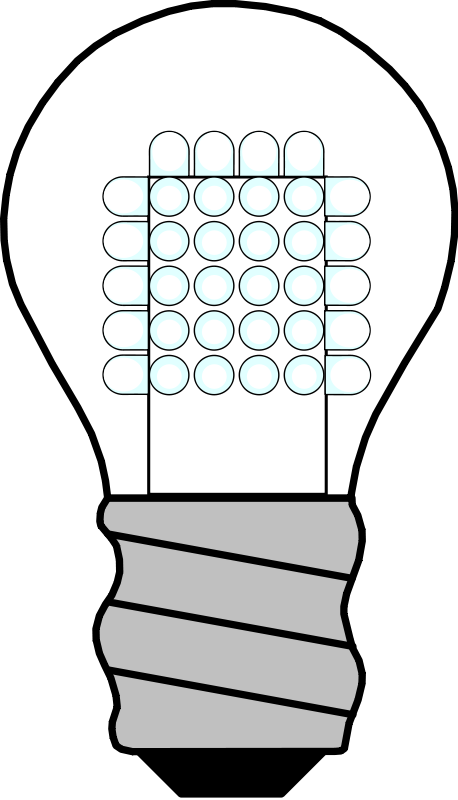
\includegraphics[scale=0.02]{imgs/bulb.png}
 \textbf{Nota} \\
 }%
{\endMakeFramed}

%Work in progress
\newenvironment{workinprogress}{%
  \def\FrameCommand{\colorbox{pink}}%
  \MakeFramed {\FrameRestore}
\lhdbend  \textbf{Work in progress} \\
 }%
{\endMakeFramed}

%Openquestion
\newenvironment{openquestion}{%
  \def\FrameCommand{\colorbox{pink}}%
  \MakeFramed {\FrameRestore}
 \textbf{Domanda aperta} \\
 }%
{\endMakeFramed}

%TODO
\newenvironment{todo}{%
  \def\FrameCommand{\colorbox{pink}}%
  \MakeFramed {\FrameRestore}
 \textbf{TODO} \\
 }%
{\endMakeFramed}

%%%%%%%%%%%%%%%%%%%%%%%%%%%%%%%%
%%%%%%%%%%%% HEADER %%%%%%%%%%%%
%%%%%%%%%%%%%%%%%%%%%%%%%%%%%%%%
\pagestyle{fancy}
% i comandi seguenti impediscono la scrittura in maiuscolo
% dei nomi dei capitoli e dei paragrafi nelle intestazioni
\renewcommand{\chaptermark}[1]{\markboth{#1}{}}
\renewcommand{\sectionmark}[1]{\markright{\thesection\ #1}}
\fancyhf{} % rimuove l'attuale contenuto dell'intestazione
% e del pi\`e di pagina
\fancyhead[LE,RO]{\bfseries\thepage}
\fancyhead[LO]{\bfseries\rightmark}
\fancyhead[RE]{\bfseries\leftmark}
\renewcommand{\headrulewidth}{0.5pt}
\renewcommand{\footrulewidth}{0pt}
\addtolength{\headheight}{0.5pt} % riserva spazio per la linea
\fancypagestyle{plain}{%
\fancyhead{} % ignora, nello stile plain, le intestazioni
\renewcommand{\headrulewidth}{0pt} % e la linea
}


%%%%%%%%%%%%%%%%%%%%%%%%%%%%%%%%
%%%%%%%%%%%% COLORS %%%%%%%%%%%%
%%%%%%%%%%%%%%%%%%%%%%%%%%%%%%%%
\definecolor{code}{gray}{0.3}


%%%%%%%%%%%%%%%%%%%%%%%%%%%%%%%%
%%%%%%%%%%%% NUMBERS %%%%%%%%%%%
%%%%%%%%%%%%%%%%%%%%%%%%%%%%%%%%
\setcounter{tocdepth}{3}
\setcounter{secnumdepth}{3}


%%%%%%%%%%%%%%%%%%%%%%%%%%%%%%%%
%%%%%%%%%%% DOC DATA %%%%%%%%%%%
%%%%%%%%%%%%%%%%%%%%%%%%%%%%%%%%
\title{Appunti di MNO}
\author{Gruppo Informatici Rampanti}
\date{ott 2010 - mag 2011}

\pdfinfo{%
  /Title    (Appunti di MNO)
  /Author   (Andrea Cimino e Lorenzo Muti)
  /Creator  (Andrea Cimino)
  /Producer (Lorenzo Muti)
  /Subject  (MNO)
  /Keywords (MNO)
}


%%%%%%%%%%%%%%%%%%%%%%%%%%%%%%%%
%%%%%%%%%%%%% UTILS %%%%%%%%%%%%
%%%%%%%%%%%%%%%%%%%%%%%%%%%%%%%%
% binary symbols
\newcommand{\modder}{\vdash _{R}}

% vertical gaps
\newcommand{\askip}{\vspace{0.5cm}}
\newcommand{\bskip}{\vspace{1.0cm}}

% various symbols
\newcommand{\qedhere}{\ensuremath{\Box}}
\newcommand{\qed}{\hfill \ensuremath{\Box}}

% substitution
\newcommand{\subst}[2]{^{#1} / _{#2}}

% denotational semantics function names
\newcommand{\bbracket}[1]{\left\llbracket #1 \right\rrbracket}

\newcommand{\aexpr}{\mathcal{A}}
\newcommand{\bexpr}{\mathcal{B}}
\newcommand{\cexpr}{\mathcal{C}}
\newcommand{\Aexpr}[1]{\mathcal{A} \bbracket{#1}}
\newcommand{\Bexpr}[1]{\mathcal{B} \bbracket{#1}}
\newcommand{\Cexpr}[1]{\mathcal{C} \bbracket{#1}}

\newcommand{\semdomset}[1]{(V_{#1})_{\bot}}

% semantic evaluations
\newcommand{\opereval}[3]{\left\langle #1, #2 \right\rangle \rightarrow #3}
\newcommand{\denaeval}[3]{\Aexpr{#1} #2 = #3}
\newcommand{\denbeval}[3]{\Bexpr{#1} #2 = #3}
\newcommand{\denceval}[3]{\Cexpr{#1} #2 = #3}

% rotated sqsubseteqs
\newcommand{\upsqsubseteq}{ $\begin{rotate}{90} $\sqsubseteq$ \end{rotate}$ }
\newcommand{\downsqsubseteq}{ $\begin{rotate}{270} $\sqsubseteq$ \end{rotate}$ }

% Space after paragraph declaration
\makeatletter
\renewcommand\paragraph{\@startsection{paragraph}{4}{\z@}%
  {-3.25ex\@plus -1ex \@minus -.2ex}%
  {1.5ex \@plus .2ex}%
  {\normalfont\normalsize\bfseries}}
\makeatother



% fast theorem and definition
\newcommand{\ftheo}[1]{\colorbox{YellowGreen}{#1}}
\newcommand{\fdefn}[1]{\colorbox{SkyBlue}{#1}}

\theoremstyle{break}
\theoremsymbol{\ensuremath{\clubsuit}}
\theoremseparator{\newline}
\newshadedtheorem{proc}[theo]{Procedura}

% bold math!
\newcommand{\bm}[1]{\mbox{\boldmath{$#1$}}}

\newcommand{\positive}[1]{\textbf{\color{green} +} #1}
\newcommand{\negative}[1]{\textbf{\color{red} -} #1}


\newtheoremlisttype{tab}%
{\begin{tabular*}{\linewidth}{@{}lrl@{\extracolsep{\fill}}r@{}}}%
{##1&##2&##3&##4\\}%
{\end{tabular*}}
\begin{document}
}
\providecommand{\outbpdocument}{\end{document}}
\else
\providecommand{\inbpdocument}{}
\providecommand{\outbpdocument}{}
\fi



\inbpdocument 

%% 25 Marzo 2011
\chapter{Il problema nonlineare dei minimi quadrati}
\section{Minimi quadrati lineari}
Analizzeremo il problema dei minimi quadrati lineari dal punto di vista
dell'ottimizzazione. Siamo nel caso continuo non vincolato:
è un problema quindi che rientra nella classe di problemi
che abbiamo studiato. Analizziamone la forma:
$$ A \in \mathbb{R}^{m \times n}, b \in \mathbb{R}^{n} \qquad
 \min \{ || Ax -b ||_{2} : x \in \mathbb{R}^{n} \} $$
Per trattare il problema, riscriviamo la funzione obiettivo:
possiamo fare la seguente equivalenza che  agevoler\`a
meglio i conti (tale riscrittura vale solo nel caso lineare)
$$ \min \{ || Ax -b ||_{2} : x \in \mathbb{R}^{n} \} 
 \equiv
 \min \left\{ \frac{1}{2} || Ax -b ||_{2}^{2} : x \in \mathbb{R}^{n} \right\}
 $$
Abbiamo fatto una scalatura ed elevato al quadrato:
i minimi in tutte e due le scritture coincidono, in quanto
le funzioni che abbiamo applicato sono monotone.
Sviluppiamo la funzione obiettivo:

$$ f(x) = \frac{1}{2} || Ax - b ||_{2}^{2} = \frac{1}{2}(Ax-b)^{T}(Ax-b) =
\frac{1}{2}x^{T} A^{T}A x - (A^{T}b)^{T}x + \frac{1}{2} b^{T}b $$
Questa \`e una  funzione quadratica, di cui sappiamo calcolare immediatamente
il gradiente 
$$ \nabla f(x) = A^{T}A x - A^{T}b $$
mentre la matrice Hessiana \`e data da :
$$ \nabla^{2}f(x) = A^{T}A$$

\paragraph{Considerazione 1: annullamento del gradiente}
Dove si annulla il gradiente?
$$ \nabla f(x) = 0 \quad
 \Longleftrightarrow \quad 
A^{T}A x = A^{T}b $$
Quest'ultimo è il sistema delle equazioni normali: i punti stazionari
sono le soluzioni delle equazioni normali. \\
Sappiamo dalla teoria che si ha minimo se la funzione è \emph{convessa},
ed \`e noto inoltre che una funzione \`e convessa se la matrice Hessiana
($\nabla^{2}f(x)$) \`e semidefinita positiva.
Andiamo quindi a controllare se abbiamo questa condizione:
$$ x^{T} A^{T}A x = (Ax)^{T}Ax = || Ax||_{2}^{2} \geq 0$$
La matrice Hessiana \`e semidefinita positiva in ogni punto, quindi
la funzione è convessa: concludiamo quindi che i punti stazionari
coincidono con i punti di minimo. Abbiamo visto il problema dei minimi quadrati sotto un altro punto di vista, quello dell'ottimizzazione.

\paragraph{Considerazione 2: matrice A di rango massimo}
Se la matrice $A$ \`e di rango massimo,
abbiamo che la funzione \`e strettamente convessa: infatti
$$
\begin{array}{c}
 A \text { rango massimo } \quad
 \Longrightarrow  \quad ( Ax=0 \Longleftrightarrow x =0 ) \quad 
 \Longrightarrow \quad  x^{T}\nabla^{2} f(x)x  > 0 \; 
\forall x \neq 0  \\
\quad \Longrightarrow \quad f \text{ strettamente convessa }
\end{array}
$$
\`E noto inoltre che, quando la funzione \`e strettamente convessa, 
esiste un solo punto di minimo.

\paragraph{Considerazione 3}
$$ f(x) = \frac{1}{2} || Ax -b||_{2}^{2} =
\frac{1}{2}\left((A_1x -b_1)^{2} + (A_2x - b_2)^{2} +
\ldots   + (A_mx -b_m)^{2})\right)$$
$f(x)$ si dice lineare quando gli addendi $ (A_mx -b_m)$ sono lineari. \\
Questo \`e il punto di partenza per parlare del problema
dei minimi quadrati non lineare.

\section{Problema dei minimi quadrati non lineare}
Un problema dei minimi quadrati non lineare ha le seguenti caratteristiche:
$$ \min \{f(x) : x \in \mathbb{R}^{n} \} \quad
f(x) = \frac{1}{2} \displaystyle \sum_{j=1}^{m} r_j^{2}(x) $$
dove
$$r_j: \mathbb{R}^{n} \rightarrow \mathbb{R} \text{ non lineari } 
\qquad  x \rightarrow A_jx-b_j;$$
Un esempio di problema non lineare era il data fitting, visto nelle
prime lezioni. I metodi per risolvere questo problema li avremmo gi\`a ma,
poich\'e conosciamo la struttura della funzione obiettivo,
vogliamo sfruttarne la struttura  per specializzare i metodi che
 abbiamo visto fino ad adesso. \\
Supporremo inoltre $r_j$ differenziabile 2 volte.\\
Cercheremo di specializzare il metodo di Newton. \\
\paragraph{Calcolo del gradiente}
La funzione $r_j^{2}$ è la composizione di $r_j$ con una funzione $\varphi$
che associa ad un valore il suo quadrato
$$ r_j^2(x) = \varphi(r_j(x)) \quad \varphi: \mathbb{R} \rightarrow \mathbb{R}
\quad t \rightarrow t^2$$
Tale funzione è derivabile e vale
$$ \varphi'(t) = 2t$$
Il gradiente di una una funzione composta \`e noto per il teorema 
(\ref{theo:derivata-funzioni-composte}) : calcoliamolo in questo caso

\begin{equation}
\label{minqbigi:001}
\nabla r_j^{2} = \nabla \varphi(r_j(x)) =
\varphi'(r_j(x)) \nabla r_j(x) = 2 r_j(x) \nabla r_j(x)
\end{equation}


Quindi, usando la linearit\`a dei gradienti e utilizzando la
(\ref{minqbigi:001}) otteniamo
$$ \nabla f(x) = \frac{1}{2}
\displaystyle \sum_{j=1}^{m} \nabla r_j^{2}(x) = 
\displaystyle \sum_{j=1}^{m} r_j(x) \nabla r_j(x) = \ldots
$$
Cerchiamo una rappresentazione pi\`u compatta:
$$ R = (r_1, \ldots, r_m): \mathbb{R}^n \rightarrow \mathbb{R}^{m}$$
$$R(x) = (r_1(x), \ldots, r_m(x)) $$
Matrice Jacobiana, le cui righe sono i gradienti dei componenti
$$J_R(x) =
\left[
\begin{array}{c}
\nabla r_1(x)^{T}\\
\vdots  \\
\nabla r_m(x)^{T}
\end{array}
\right]
\in \mathbb{R}^{m \times n}
 $$

Il tutto si riduce quindi a:
$$ \nabla f(x) = \ldots = J_R(x)^{T}R(x)$$

\paragraph{Calcolo della matrice hessiana}
Calcoliamo le derivate seconde, la matrice hessiana di $f$
$$[ \nabla^{2}f(x)]_{kl} = 
\frac{\partial^{2} f(x)}{\partial x_k \partial x_l}=
\frac{\partial}{\partial x_k}\left(\frac{\partial f}{\partial x_l}(x)\right) =
\frac{\partial}{\partial x_k }
\left(\displaystyle \sum_{j=1}^{m} r_j(x) 
\frac{\partial r_j}{\partial x_l}(x) \right)
\underbracket{=}_{*)}
\displaystyle \sum_{j=1}^{m}
\underbracket{\frac{\partial r_j(x)}{\partial x_k} 
\frac{\partial r_j(x)}{\partial x_l}}_{[J_R(x)^{T}J_{R}(x)]_{kl}}
+ \displaystyle \sum_{j=1}^{m} r_j(x)
\underbracket{\frac{\partial^{2}r_j(x)}{\partial x_k \partial x_l}}_{[\nabla^{2} r_j(x)]_{kl}}
$$
\begin{notes}
 *) Si sta applicando la regola di derivazione del prodotto.
\end{notes}

$$
[J_R(x)^{T}J_{R}(x)]_{kl} = 
\left[
\begin{array}{ccc}
\nabla r_1(x)^{T}  & \cdots &  \nabla r_m(x)^{T} \\
\end{array}
\right]
\left[
\begin{array}{c}
\nabla r_1(x)^{T}\\
\vdots  \\
\nabla r_m(x)^{T}
\end{array}
\right]
$$\

In forma matriciale possiamo riscrivere tutto come
$$ \nabla^{2}f(x) = J_R(x)^{T}J_R(x) + 
 \displaystyle \sum_{j=1}^{m} r_j(x) \nabla^{2} r_j(x)$$
Poich\'e abbbiamo le formule esplicite del gradiente e della matrice
hessiana, possiamo sostituirle nei metodi visti
specializzarli.  Ad esempio nel metodo di Newton \ref{newtongradesatto}: $d^{k} \in
\mathbb{R}^{n}$ soluzione del sistema
$$ \nabla^{2}f(x^{k})d = - \nabla f(x^{k}) $$
Se $\nabla^{2} f(x^{k})$ è definita positiva, allora $d_{N}^{k}$ è una
direzione di discesa.  Cercheremo un'approssimazione del metodo di
Newton per togliere di mezzo i termini del secondo ordine: otterremo
il metodo di Gauss-Newton, per evitare il calcolo delle matrice
hessiane.

\section{Metodo di Gauss-Newton}
Vogliamo cercare di approssimare quindi le matrici hessiane con 
la parte del primo ordine, che domina la parte del secondo
ordine quando i residui sono piccoli.

\paragraph{Notazioni}
Cerchiamo delle notazioni comode per fare le nostre
considerazioni
$$ J_k = J_{R}(x^{k}), \quad R_k = R(x^k)= (r_1(x^{k}), \ldots,
r_n(x^{k}))
\quad
\text{ Funzioni residuali:$r_j$
}
$$
Il gradiente \`e definito nel seguente modo
$$ \nabla f(x^{k}) = J_{k}^{T}r_k,\quad$$
mentre la matrice hessiana viene approssimata
come segue
$$\nabla^{2}f(x^{k}) \approx J_k^{T}J_k $$
Il metodo di Gauss-Newton 
$$ d^{k}_{GN} \in \mathbb{R}^{n} 
\text{ soluzione di } \underbracket{J_{k}^{T}J_kd = - J_k^{T}r_k}_{\text{sistema lineare}}$$
Mentre nel metodo di Newton standard per avere una direzione di discesa
era necessario che la matrice hessiana fosse definita positiva,
qui invece le condizioni sono meno strette.
Vale infatti il seguente teorema:

\begin{theo}
Se $\nabla f(x^{k}) \neq 0$, allora $d_{GN}^{k}$ è una direzione
di discesa
\end{theo}
\begin{thproof}
Facciamo una serie di sostituzioni
$$ 
\begin{array}{l}
\nabla f(x^{k})^{T}d_{GN}^{k} = 
(J_k^{T}r_k)^{T} d_{GN}^{k}  \underbracket{=}_{\text{sistema lineare}} 
-(J_k^{T} J_{k} d_{GN}^{k})^{T} d_{GN}^{k} = \\
\underbracket{=}_{\text{reverse order law}} 
-(J_{k}^{T} d_{GN}^{k})^{T}(J_{k}d_{GN}^{k})
= - ||J_k^{T} d_{GN}^{k}||_{2}^{2} \leq 0 
\end{array}
$$
Affinch\'e si abbia una direzione di discesa,
la quantit\`a deve essere minore di zero.
Ma se
$$ J_{k}^{T} = d_{GN}^{k} = 0 \rightarrow
J_{k}^{T}r_k = 0 \text{ abbiamo } \nabla f(x^{k}) = 0 $$
Quindi quando il gradiente non \`e zero, abbiamo una
direzione di discesa.
\end{thproof}

\paragraph{Legame tra Gauss Newton e minimi quadrati}
$$J_{k}^{T}J_kd = - J_k^{T}r_k$$
inoltre è il sistema delle equazioni normali associate al sistema
$J_kd + r_k=0 $, ovvero la direzione di Newton $d_{GN}^{k}$ è la
soluzione di un problema di minimi quadrati lineare, risolve il
problema dei minimi quadrati lineari
$$ \min \left\{ \frac{1}{2} || J_k d + r_k ||_{2}^{2} \quad d \in \mathbb{R}^{n} \right\} $$
Trovare quindi una direzione di Gauss Newton, corrisponde
a risolvere un problema dei minimi quadrati,
e conosciamo tre metodi che non richiedono
il calcolo della matrice hessiana. \\ \\
Possiamo analizzare il metodo anche da un'altro punto di vista, calcoliamo lo sviluppo di Taylor del primo ordine di $r_j(x^{k}+ d) $:
$$ r_j(x^{k}+ d)  \approx r_j(x^{k}) + \nabla r_j(x^{k})^{T} d$$
$$ f(x^k + d) = 
\frac{1}{2} \displaystyle \sum_{j=1}^{n} r_j^{2}(x^{k} + d) \approx
 \frac{1}{2} \displaystyle \sum_{j=1}^{m}
\left[ r_j(x^{k}) + \nabla r_j(x^{k})^{T}d\right]^{2} = 
\frac{1}{2} || r_k + J_kd ||_{2}^{2} $$
Quindi $d_{GN}^{k}$ si ottiene minimizzando questa approssimazione di $f(x^k + d)$. \\ \\

Potremmo pensare passi unitari in stile Newton, ma in questo caso
non sarebbe garantita la convergenza del metodo: bisogna aggiungere
una ricerca inesatta del passo.

\paragraph{Metodo di Gauss-Netwon (``damped GN'')}
\begin{enumerate}
\item si sceglie un punto $x_0 \in \mathbb{R}^{n}$, $k=0$
\item se $\nabla f(x)=0$ (il punto trovato è stazionario),
      allora STOP.
\item altrimenti dobbiamo calcolare $d^{k}_{GN} \in \mathbb{R}^{n}$ soluzione
      di $J_{k}^{T}J_{k}d = -J_{k}R_{k}$
\item calcolare $t_k > 0 $ che soddisfi le condizioni di Wolfe
\item $x^{k+1} = x^{k} + t_k d_{GN}^{k}$
\item $k = k+1$ e tornare a 2)
\end{enumerate}

\begin{theo}[Teorema di convergenza]
Supponiamo che 
\begin{itemize}
\item $L_f(x^{0}) = \{ x \in \mathbb{R}^{n} : f(x) \leq f(x^{0}) \}$
     (curve di sottolivello) sia compatto
\item $r_j$ siano differenziabili con continuit\`a  per ogni $j=1\ldots n$
 \item $\nabla f$ sia continua di tipo Lipschitziano
\item $\exists \gamma > 0  \text{ t.c. } || J_kz||_{2} \geq \gamma ||z||_{2} 
\quad \forall z \in \mathbb{R}^{n} \; \forall k \text{ (iterazioni del metodo)} \quad (***)$ 
\end{itemize}
Allora 
$$ \lim_{k \to +\infty} || \nabla f(x^{k})||_{2} = 0 $$
\end{theo}
Vediamo il significato dell'ultima ipotesi:
ci garantisce che i valori singolari di $J_k$ siano uniformemente
distanti da 0.
Cerchiamo di capire perch\'e: sia
$ z=v_i $ vettore singolare destro di $J_k$: ha norma 1
$$ || J_k v_i||_{2} = \sigma_i \quad \sigma_i \geq \gamma \text{ per ogni
matrice } J_k $$
Quindi per ogni iterazione del metodo tutti i valori singolari saranno maggiori di $\gamma$.
\\
($\sigma_i$: valori singolari)
\begin{thproof}
\begin{todo}
Fare rivedere a Bigi la dimostrazione
\end{todo}
Per ipotesi $x \rightarrow J_r(x)$ è una funzione continua.
Allora $x \rightarrow || J_R(x)||_{2}$ continua, poich\'e
la norma \`e continua.
La curva di sottolivello $L_{f}(x^{0})$  per ipotesi \`e compatta.
Allora, per il teorema di Weirstrass esiste un massimo
$$ \exists \; \beta > 0 \quad 
|| J_{R}(x)||_{2} \leq \beta \quad \forall x \in L_f(x^{0}) 
$$
Sia $\theta_k$ l'angolo tra $-\nabla f(x^{k})$ e $d_{GN}^{k}$.
Abbiamo
$$ \cos \theta_{k} = 
\frac{-f(x^{k})^{T}d_{GN}^{k}}{|| \underbracket{\nabla f(x^{k})}_{(*)}||_{2} 
\; ||d_{GN}^{k}||_{2}} =
 \frac{|| J_{k}^{T}d_{GN}^{k} ||_{2}^{2} }{|| \underbracket{J_{k}^{T}J_k d_{GN}^{k}}_{(*)}||_{2}
||d_{GN}^{k}||_{2} } \geq \ldots (**)
$$
Valgono
\begin{itemize}
\item $ J_k^{T}r_k = -J_k^{T}J_{k}d_N^{k} \qquad (*)$
\item 
$
 || J_k^{T} J_k d_{GN}^{k}||_{2} \leq || J_{k} ||_{2}^{2}||d_{GN}^{k}||_{2}
\leq \beta^{2} ||d_{GN}^{k}||_{2} \qquad (**)
$
\end{itemize}
$$ \ldots \geq
\frac{|| J_k^{T} d_{GN}^{k}||_{2}^{2}}{\beta^{2} ||d^{k}_{GN}||_{2}^{2}}
\underbracket{\geq}_{(***)} \frac{\gamma^{2}||d_{GN}^{k}||_{2}^{2}}{\beta^{2} ||d_{GN}||{2}^{2}}$$
Dato Wolfe, Lipschitziana, funzione limite 
$$
\displaystyle \sum_{k=0}^{\infty} \underbracket{\cos^{2} \theta_k}_{\neq 0} || \nabla f(x^{k})||^{2} < + \infty \quad \Longrightarrow \quad \lim_{k \to + \infty} || \nabla f(x^{k})||_{2} = 0$$
\end{thproof}
In realt\`a  la condizione di Lipschitziana non è necessaria.


%% Da qui parte non revisionata
%% 29 Marzo 2011
\section{Regressioni (non) lineari - data/curve fitting}
Contesto: immaginiamo di avere un gruppo di dati, istanti di
tempo 
$$ y \in \mathbb{R}\; t_j \in \mathbb{R}^{p} $$
Vediamo se ci sono delle correleazioni tra i $t_j$
e gli $y$.
L'idea è avere una black box che prende in input
i $t_j$ e sputa fuori i $t_j$
$$ y \approx f(\underbracket{t_j}_{\text{ regressori }})$$
Per cercare di capire il comportamento della black box
possiamo fare
$$
\min\left\{ \frac{1}{2}
\left(\displaystyle \sum_{j=1}^{m} [y_j - f(t_j)]^{2} \right)
; \quad f \in T
\right\}
$$
Non abbiamo un vettore come incognita, abbiamo un insieme di funzioni.
In $\mathbb{R}^{n}$ abbiamo una base finita, nello spazio
di funzioni abbiamo una base infinita, le variabili sono
delle funzioni. Questo argomento non fa parte del corso.
Cerchiamo però di vedere un esempio.
$$ T = \{ f(x_1,\ldots, x_m; \cdot) :
\underbracket{x_1, x_2, \ldots, x_n}_{\text{parametri}} \in \mathbb{R}  \}$$
Assegnato il valore ad un insieme finito di parametri,
otteniamo la funzione corrispondente.
Abbiamo quindi ristretto l'insieme delle funzioni che è possibile
considerare, questo per un discorso di rappresentazione.
Basta riprendere l'esempio della prima lezione
di curve fitting per avere un esempio concreto.
Il nuovo problema è espresso come
$$ \min \left\{ \frac{1}{2} 
\displaystyle \sum_{j=1}^{n}[y_j - f(x_1,\ldots, x_n)]^{2}\; : \;
x_1, x_2, \ldots, x_n \in \mathbb{R} \right\}
$$
Esempio: Modello di crescita di un nuovo servizio.
si vuole ottenere un modello.
Vari modelli di crescita:
\begin{itemize}
\item Crescita esponenziale: $eg(t)  = x_1 e^{x_2 t}$
\item Potenza temporale: $tp(t)= x_1t^{x_2}$
 \item Crescita limitata $lmg(t) = x_3 - x_1^{-x_2 t}$
\item Logistica: $lgs(t) = x_3 / (1 + x_1 e^{-x_2 t})$
\end{itemize}
I primi due non hanno un bound superiore, le ultime due si.
Nell'esempio abbiamo gli ultimi 3 modelli ad essere
candidati.

$$
 \min \left\{ \frac{1}{2} 
\displaystyle \sum_{j=1}^{n}[y_j - tp(x_1,x_2;t_j)]^{2}\; : \;
x_1, x_2 \in \mathbb{R} \right\}
$$
$$ tp(x_1,x_2,t) = x_1 t^{x_2}$$
Nella lezione avevamo gli elementi residuali scritti come
$$ r_j(x_1, x_2) = y_j - x_1 t_j^{x_2}$$
Abbiamo 36 funzioni residuali candidate, e si può
utilizzare Gauss Newton per risolvere il problema.
\texttt{lsqnonlin} in Matlab.
Da notare che nella teoria, come criterio d'arresto
abbiamo
$$\nabla f(x^{*})=0$$
nella pratica si utilizza
\begin{itemize}
\item $ || \nabla f(x^{k})|| \leq \text{ tol } $
 \item $ |f(x^{k-1}) - f(x^{k})| \leq \text{ tol } $
\end{itemize}
Secondo caso
$$
 \min \left\{ \frac{1}{2} 
\displaystyle \sum_{j=1}^{n}[y_j - lmg(x_1,x_2;t_j)]^{2}\; : \;
x_1, x_2 , x_3 \in \mathbb{R} \right\}
$$

$$ tp(x_1,x_2, x_3, t) =x_3 - x_1 e^{-x_2 t}$$
Ultimo caso: funzione logistica

$$
 \min \left\{ \frac{1}{2} 
\displaystyle \sum_{j=1}^{n}[y_j - lmg(x_1,x_2;t_j)]^{2}\; : \;
x_1, x_2, x_3 \in \mathbb{R} \right\}
$$

$$lgs(x_1,x_2, x_3, t) =x_3 /(1+x_1e^{-x_2t})$$

\outbpdocument

 %% Bigi: minimi quadrati
 %% Copyright (C) 2011, Andrea Cimino, All Rights Reserved.
 %% This file is distributed under the terms of the Creative Commons
 %% Licence Non-Commercial Share-Alike license


%% Useful stuff for separate compilation.
\ifx\ismaindoc\undefined
\providecommand{\inbpdocument}{
 \documentclass[11pt,a4paper,twoside,titlepage]{scrbook}
%%%%%%%%%%%%%%%%%%%%%%%%%%%%%%%%
%%%%%%%%%%% PACKAGES %%%%%%%%%%%
%%%%%%%%%%%%%%%%%%%%%%%%%%%%%%%%
% encoding
\usepackage[utf8x]{inputenc}
\usepackage[italian]{babel} % babel (suddivisione parole in sillabe)

\usepackage{amsfonts} % matematica
\usepackage{amsmath} % matematica
\usepackage{amssymb} % simboli vari
\usepackage{calrsfs}
\usepackage{caption}
\usepackage{enumerate}
\usepackage{extarrows} % matematica
\usepackage{keyval}
\usepackage{manfnt} % Simboli curva
\usepackage{mathtools} % matematica
\usepackage{multirow} 
\usepackage[usenames, dvipsnames]{color} % colori con nome
\usepackage[pdftex]{graphicx}
\usepackage{epstopdf} % gestione file EPS
\usepackage{wrapfig} % per figure circondate da testo
\usepackage{framed}	% teoremi framed
\usepackage{fancyhdr} % header buffi
\usepackage[T1]{fontenc} % gestione hbox e vbox
\usepackage[a4paper]{geometry}
\usepackage{microtype} % gestione hbox e vbox
\usepackage[thref, amsthm, amsmath, framed, hyperref]{ntheorem} % teoremi (avanzata)
%% \usepackage{prooftree} % gestione prof-tree
\usepackage{rotating}
\usepackage{stmaryrd}
\usepackage{subfig}
\usepackage{syntax} % syntattic stuff
\usepackage{txfonts}
\usepackage{verbatim} % migliorie al verbatim
%\usepackage{hyperref}
%% \usepackage{qtree}
\usepackage{fancyvrb}
\usepackage{listings}
\usepackage{cancel}
\usepackage{tikz}

\usepackage{bbding} %% Icons

%%%%%%%%%%%%%%%%%%%%%%%%%%%%%%%%
%%%%%%%%%%% GEOMETRY %%%%%%%%%%%
%%%%%%%%%%%%%%%%%%%%%%%%%%%%%%%%
\geometry{verbose,tmargin=2cm,bmargin=2.5cm,lmargin=2.5cm,rmargin=2cm}
\parindent0ex %% Remove paragraph indenting

%%%%%%%%%%%%%%%%%%%%%%%%%%%%%%%%
%%%%%%%%%%% CODE ENV %%%%%%%%%%%
%%%%%%%%%%%%%%%%%%%%%%%%%%%%%%%%
% codice
\newcounter{count}
\setcounter{count}{0}
\newenvironment{code}[1]
{
\color{lightgray}\hrulefill\color{code}
\stepcounter{count} {\bf\small Listato di codice \arabic{count}: {#1} }
\verbatim
}
{
\endverbatim
\color{lightgray}\hrulefill
\color{black}
\\
}

% codice semplice
\newenvironment{simplecode}
{
\color{code} \tt
}
{
\rm
}

 % Notation issues
\input{macros}

\makeatletter
\g@addto@macro\@verbatim\footnotesize
\makeatother



%%%%%%%%%%%%%%%%%%%%%%%%%%%%%%%%
%%%%%%%% THEOREMS FORMAT %%%%%%%
%%%%%%%%%%%%%%%%%%%%%%%%%%%%%%%%
% shaded theorems and proofs command
\definecolor{lightgray}{RGB}{230,230,230}
\def\theoremframecommand{\colorbox{lightgray}}

%%% theorems
\theoremstyle{break}
\theoremheaderfont{\normalfont\bfseries}
\theorembodyfont{\itshape}
\theoremsymbol{\ensuremath{\diamondsuit}}
\theoremseparator{\newline}
\newtheorem{theo}{
\includegraphics[scale=0.11]{imgs/book.png}Teorema}[chapter]

%%% propositions
\theoremstyle{break}
\theoremheaderfont{\normalfont\bfseries}
\theorembodyfont{\itshape}
\theoremsymbol{\ensuremath{\diamondsuit}}
\theoremseparator{\newline}
\newshadedtheorem{proposition}{Proposizione}[chapter]

%%% exercises
\theoremstyle{break}
\theoremheaderfont{\normalfont\bfseries}
\theorembodyfont{\itshape}
\theoremsymbol{\ensuremath{\diamondsuit}}
\theoremseparator{\newline}
\newshadedtheorem{exercise}{Esercizio}[chapter]

%%% propositions
\theoremstyle{break}
\theoremheaderfont{\normalfont\bfseries}
\theorembodyfont{\itshape}
\theoremsymbol{\ensuremath{\diamondsuit}}
\theoremseparator{\newline}
\newshadedtheorem{property}{\PencilRightDown $\; $ Propriet\`a}[chapter]

%%% lemmas
\theoremstyle{break}
\theoremheaderfont{\normalfont\bfseries}
\theorembodyfont{\itshape}
\theoremsymbol{\ensuremath{\diamondsuit}}
\theoremseparator{\newline}
\newshadedtheorem{lemma}[theo]{Lemma}

%%% definitions
\theoremstyle{break}
\theoremsymbol{\ensuremath{\clubsuit}}
\theoremseparator{\newline}
\newshadedtheorem{defn}[theo]{Definizione}

%%% examples
\theoremstyle{break}
\theorembodyfont{\itshape}
\theoremsymbol{\ensuremath{\ast}}
\theoremseparator{\newline}
\newshadedtheorem{example}[theo]{Esempio}

%%% observations
\theoremstyle{break}
\theorembodyfont{\itshape}
\theoremsymbol{\ensuremath{\ast}}
\theoremseparator{\newline}
\newshadedtheorem{observation}[theo]{

\includegraphics[scale=0.06]{imgs/lens.png}
Osservazione
}

%%% notations
\newtheorem*{notaz}{Notazione}

%%% proofs
\newenvironment{thproof}
{
\vskip 0.03cm
\begin{small}
\textit{Dimostrazione. }
\color{code}
}
{
\color{black}
\end{small}
$ \square $
\vskip 0.2cm
}

%Notes
\newenvironment{notes}{%
  \def\FrameCommand{\colorbox{yellow}}%
  \MakeFramed {\FrameRestore}
\includegraphics[scale=0.02]{imgs/bulb.png}
 \textbf{Nota} \\
 }%
{\endMakeFramed}

%Work in progress
\newenvironment{workinprogress}{%
  \def\FrameCommand{\colorbox{pink}}%
  \MakeFramed {\FrameRestore}
\lhdbend  \textbf{Work in progress} \\
 }%
{\endMakeFramed}

%Openquestion
\newenvironment{openquestion}{%
  \def\FrameCommand{\colorbox{pink}}%
  \MakeFramed {\FrameRestore}
 \textbf{Domanda aperta} \\
 }%
{\endMakeFramed}

%TODO
\newenvironment{todo}{%
  \def\FrameCommand{\colorbox{pink}}%
  \MakeFramed {\FrameRestore}
 \textbf{TODO} \\
 }%
{\endMakeFramed}

%%%%%%%%%%%%%%%%%%%%%%%%%%%%%%%%
%%%%%%%%%%%% HEADER %%%%%%%%%%%%
%%%%%%%%%%%%%%%%%%%%%%%%%%%%%%%%
\pagestyle{fancy}
% i comandi seguenti impediscono la scrittura in maiuscolo
% dei nomi dei capitoli e dei paragrafi nelle intestazioni
\renewcommand{\chaptermark}[1]{\markboth{#1}{}}
\renewcommand{\sectionmark}[1]{\markright{\thesection\ #1}}
\fancyhf{} % rimuove l'attuale contenuto dell'intestazione
% e del pi\`e di pagina
\fancyhead[LE,RO]{\bfseries\thepage}
\fancyhead[LO]{\bfseries\rightmark}
\fancyhead[RE]{\bfseries\leftmark}
\renewcommand{\headrulewidth}{0.5pt}
\renewcommand{\footrulewidth}{0pt}
\addtolength{\headheight}{0.5pt} % riserva spazio per la linea
\fancypagestyle{plain}{%
\fancyhead{} % ignora, nello stile plain, le intestazioni
\renewcommand{\headrulewidth}{0pt} % e la linea
}


%%%%%%%%%%%%%%%%%%%%%%%%%%%%%%%%
%%%%%%%%%%%% COLORS %%%%%%%%%%%%
%%%%%%%%%%%%%%%%%%%%%%%%%%%%%%%%
\definecolor{code}{gray}{0.3}


%%%%%%%%%%%%%%%%%%%%%%%%%%%%%%%%
%%%%%%%%%%%% NUMBERS %%%%%%%%%%%
%%%%%%%%%%%%%%%%%%%%%%%%%%%%%%%%
\setcounter{tocdepth}{3}
\setcounter{secnumdepth}{3}


%%%%%%%%%%%%%%%%%%%%%%%%%%%%%%%%
%%%%%%%%%%% DOC DATA %%%%%%%%%%%
%%%%%%%%%%%%%%%%%%%%%%%%%%%%%%%%
\title{Appunti di MNO}
\author{Gruppo Informatici Rampanti}
\date{ott 2010 - mag 2011}

\pdfinfo{%
  /Title    (Appunti di MNO)
  /Author   (Andrea Cimino e Lorenzo Muti)
  /Creator  (Andrea Cimino)
  /Producer (Lorenzo Muti)
  /Subject  (MNO)
  /Keywords (MNO)
}


%%%%%%%%%%%%%%%%%%%%%%%%%%%%%%%%
%%%%%%%%%%%%% UTILS %%%%%%%%%%%%
%%%%%%%%%%%%%%%%%%%%%%%%%%%%%%%%
% binary symbols
\newcommand{\modder}{\vdash _{R}}

% vertical gaps
\newcommand{\askip}{\vspace{0.5cm}}
\newcommand{\bskip}{\vspace{1.0cm}}

% various symbols
\newcommand{\qedhere}{\ensuremath{\Box}}
\newcommand{\qed}{\hfill \ensuremath{\Box}}

% substitution
\newcommand{\subst}[2]{^{#1} / _{#2}}

% denotational semantics function names
\newcommand{\bbracket}[1]{\left\llbracket #1 \right\rrbracket}

\newcommand{\aexpr}{\mathcal{A}}
\newcommand{\bexpr}{\mathcal{B}}
\newcommand{\cexpr}{\mathcal{C}}
\newcommand{\Aexpr}[1]{\mathcal{A} \bbracket{#1}}
\newcommand{\Bexpr}[1]{\mathcal{B} \bbracket{#1}}
\newcommand{\Cexpr}[1]{\mathcal{C} \bbracket{#1}}

\newcommand{\semdomset}[1]{(V_{#1})_{\bot}}

% semantic evaluations
\newcommand{\opereval}[3]{\left\langle #1, #2 \right\rangle \rightarrow #3}
\newcommand{\denaeval}[3]{\Aexpr{#1} #2 = #3}
\newcommand{\denbeval}[3]{\Bexpr{#1} #2 = #3}
\newcommand{\denceval}[3]{\Cexpr{#1} #2 = #3}

% rotated sqsubseteqs
\newcommand{\upsqsubseteq}{ $\begin{rotate}{90} $\sqsubseteq$ \end{rotate}$ }
\newcommand{\downsqsubseteq}{ $\begin{rotate}{270} $\sqsubseteq$ \end{rotate}$ }

% Space after paragraph declaration
\makeatletter
\renewcommand\paragraph{\@startsection{paragraph}{4}{\z@}%
  {-3.25ex\@plus -1ex \@minus -.2ex}%
  {1.5ex \@plus .2ex}%
  {\normalfont\normalsize\bfseries}}
\makeatother



% fast theorem and definition
\newcommand{\ftheo}[1]{\colorbox{YellowGreen}{#1}}
\newcommand{\fdefn}[1]{\colorbox{SkyBlue}{#1}}

\theoremstyle{break}
\theoremsymbol{\ensuremath{\clubsuit}}
\theoremseparator{\newline}
\newshadedtheorem{proc}[theo]{Procedura}

% bold math!
\newcommand{\bm}[1]{\mbox{\boldmath{$#1$}}}

\newcommand{\positive}[1]{\textbf{\color{green} +} #1}
\newcommand{\negative}[1]{\textbf{\color{red} -} #1}


\newtheoremlisttype{tab}%
{\begin{tabular*}{\linewidth}{@{}lrl@{\extracolsep{\fill}}r@{}}}%
{##1&##2&##3&##4\\}%
{\end{tabular*}}
\begin{document}
}
\providecommand{\outbpdocument}{\end{document}}
\else
\providecommand{\inbpdocument}{}
\providecommand{\outbpdocument}{}
\fi



\inbpdocument 

%% Bigi 1 Aprile
\chapter{Ottimizzazione vincolata con regione ammissibile convessa}
Fino ad adesso abbiamo considerato il caso senza vincoli.
Nel caso vincolato il problema diventa:
$$(P) \quad \min \left\{ f(x) : x \in X \right\} \quad
f:\mathbb{R}^{n} \rightarrow \mathbb{R}
\quad X \subseteq \mathbb{R}^{n}
$$
Sono 2 i casi che andremo ad analizzare
\begin{itemize}
 \item  Caso di un $X$ generico
 \item  Caso di un $X$ esplicitamente descritto da  disuguaglianze e uguaglianze. In
    questo caso la descrizione della regione ammissibile \`e la seguente:
     $$ X = \{ x \in \mathbb{R}^{n} \; | \; g_i(x) \leq 0, i =1\ldots n, \; h_j(x)=0, j=1 \ldots p \} $$
     
\end{itemize}


\begin{example}[Reti di traffico]

Attraversamento di un arco al variare del flusso.
Maggiore \`e la quantit\`a di traffico attraverso un arco, maggiore \`e il tempo
di percorrrenza. Vogliamo minimizzare il tempo di percorrenza nella rete.

\begin{center}
  \includegraphics[scale=0.6]{imgs/traffico.png}
\end{center}

Un esempio di funzione che descrive la quantit\`a di tempo necessaria a percorrere
l'arco $ij$ \`e la seguente:
$$
t_{ij}(v) = t_{ij} + \alpha _{ij}  \frac{v}{c_{ij} - v} \quad  (v < c_{ij}) \qquad
\left \{
\begin{array}{ll}
 t_{ij}, \alpha _{ij} & \text{ costanti relative al tipo di strada} \\
 c_{ij}: & \text{ capacit\`a  in } ij \\
 v:  & \text{ volume di traffico attuale} 
\end{array}
\right.
$$
Un'altra funzione possibile per descrivere il tempo di attraversamento al variare del volume 
di traffico \`e 
$$
t_{ij}(v) = t_{ij} + \alpha_{ij} \dfrac{v_j}{c_{ij}^{4}}
$$
dove $c_{ij}$ non \`e la capacit\`a!
La funzione obiettivo da minimizzare \`e:
$$ \min \displaystyle \sum_{(i,j)} x_{ij} t_{ij} (x_{ij}) $$
Il problema questa volta \`e  vincolato:  abbiamo dei vincoli di conservazione del flusso
ossia, la quantit\`a di traffico che entra da un nodo deve essere uguale a quella che esce.\
La regione ammissibile \`e descritta da:
$$
\left\{
\begin{array}{l}
x_{12} + x_{13} = d               \\
x_{24} + x_{34} =d                \\
x_{12} + x_{32} = x_{23} + x_{24} \\
x_{13} + x_{23} = x_{32} + x_{34} \\
x_{ij} \geq 0                     \\
 (x_{ij} \leq c_{ij}) \quad  (\text{opzionale: capacit\`a limitata su un arco})
\end{array}
\right.
$$
Il problema pu\`o essere descritto pi\`u in generale dalla seguente notazione
basata su grafi:
$$
\displaystyle
\sum_{j \in BN(i)} x_{ji}
-
\displaystyle
\sum_{j \in FN(i)} x_{ji}
=
\left\{
\begin{array}{cl}
  -d & i = 0                      \\
  0  & i \neq 0,t                 \\
  d  & i = t
\end{array}
\right.
$$
\end{example}

\section{Condizioni di ottimalit\`a con regione ammissibile convessa}
Come facciamo a sapere se l'insieme \`e convesso?
$$ X = \{ x \in \mathbb{R}^{n} \; : \; g_{i}(x) \leq 0, h_j(x)=0 \} $$
$$
i=1\ldots n \quad j=1\ldots p
\quad
g_i : \mathbb{R}^{n} \rightarrow \mathbb{R}
\quad
h_i : \mathbb{R}^{n} \rightarrow \mathbb{R}
$$
Le funzioni $g_i$ (vincoli di disuguaglianza) e $h_j$ (vincoli di
uguaglianza) definiscono i vincoli applicabili su $\mathbb{R}^n$ per
definire la regione ammissibile.
La natura delle funzioni vincolari pu\`o garantire la convessita di $X$.
% Quando riusciremo ad avere un insieme convesso?

\begin{defn}[Funzione affine]
Una funzione $h_j$ si dice \emph{affine} se
$$ h_j(x) = a_{j}^{T}x + b_j
\qquad
a_j \in \mathbb{R}^{n}, b_j \in \mathbb{R}
$$
\end{defn}

\begin{proposition}
Se le funzioni $g_i$ sono convesse per $i=1\ldots n$ e le funzioni
$h_j$ sono affini per $j=1\ldots p$, allora $X$ \`e un insieme convesso
\end{proposition}
\begin{thproof}
Si sfrutta la definizione di convessit\`a. Si prendano
$x,y \in X$ e $\lambda \in [0,1]$.
Il segmento che unisce i due punti \`e dato da
$$ \lambda x + (1- \lambda )y$$
\begin{itemize}
\item Vincoli di disuguaglianza:
$$ g_i(\lambda x + (1-\lambda) y)
\leq
\lambda \underbracket{ g_i(x)}_{\leq 0}
+ (1- \lambda) \underbracket{ g_i(y)}_{\leq 0}
\; \leq \;  0
$$
\begin{notes}
$g_i(x) \leq 0$ e $g_i(y) \leq 0$ in quanto per ipotesi apparengono ad
$X$: se non fosse cos\`i $x$ ed $y$ sarebbero fuori dalla regione
ammissibile.
\end{notes}
\item
Vincoli di uguaglianza:
$$
\begin{array}{lr}
  h_j(\lambda x + (1-\lambda)y) = & \\
  a_j^{T}(\lambda x + (1-\lambda)y)+ b_j = & [\; \text{ponendo } b_j = 
  \lambda b_j + (1-\lambda) b_j  \; ]   \\
  \lambda a_{j}^{T}x + (1-\lambda) a_{j}^{T}y+ 
  \lambda b_j + (1-\lambda) b_j = \\
  \lambda \underbracket{h_j(x)}_{=0} + (1-\lambda) \underbracket{h_j(y)}_{=0} = 0
\end{array}
$$
\begin{notes}
$g_i(x) = 0$ e $g_i(y) =  0$ in quanto per ipotesi apparengono ad
$X$.
\end{notes}
\end{itemize}


\end{thproof}
Per avere un algoritmo, dobbiamo stabilire le condizioni di ottimalit\`a:
minimo locale e globale. \\
L'ipotesi che assumiamo \`e che $f$ sia differenziabile, in modo
che si possano utilizzare i gradienti e le matrici hessiane. \\
Le condizioni di ottimalit\`a che abbiamo visto nel caso non vincolato,
valgono anche nel caso vincolato?

\begin{example}
Vediamo in esempio in cui dimostriamo che le condizioni di ottimalit\`a
viste nel caso non vincolato non sono pi\`u sufficienti.
Vogliamo minimizzare la funzione
$$ f(x) =  x_1^{2} + x_2^{2}
\qquad
X = [1,2] \times [0,1]
$$
\begin{center}
  \includegraphics[width=0.3\textwidth]{imgs/vincolocos.png}
\end{center}

Nel caso non vincolato il minimo \`e in $(0,0)$
ed il gradiente di $f$ \`e
$$ \nabla f(x) = 2x$$
Il gradiente si annulla nel caso del vettore $x=0$,
ma $x \notin X$.
\end{example}

Questo esempio quindi dimostra che
questa non pu\`o essere la condizione di ottimalit\`a:
bisogna cercare una differente nozione di punto stazionario.

\begin{defn}[Direzione ammissibile]
Un vettore $d \in \mathbb{R}^{n}$ si dice
\emph{direzione ammissibile} per
$X$ a partire da $\overline{x} \in X$
se  $\exists \overline{t} > 0 \text{  tale che  }$
$$
x(t) = \overline{x} + td \in X \quad
\forall t \in [0,\overline{t}]
$$
\end{defn}
Se $d$ \`e una direzione ammissibile, anche i suoi
multipli sono ancora una direzione ammissibile.\\
L'insieme in cui appartengono anche i suoi multipli
si chiama \emph{cono}.

\begin{defn}[Cono delle direzioni ammissibili]
$$ F(X, \overline{x}) = \{
d \in \mathbb{R}^{n}\; : \;
\exists \overline{t}> 0 \; \text{tale che} \;
\overline{x} + td \in X \quad \forall t \in [0,\overline{t}] \; \}
$$
\end{defn}

\begin{observation}
Se $d$ appartiene alla regione ammissibile, anche tutti i suoi multipli ci appartengono.
\end{observation}

\begin{observation}
Se $\overline{x}$ \`e un punto \emph{interno} a $X$, allora
$$F(X,\overline{x}) = \mathbb{R}^{n}$$
\end{observation}

L'idea quindi \`e quella di testare l'ottimalita lungo tutte
le direzioni ammissibili.

\begin{theo}[Condizione necessaria]
\label{ottvinc:01}
 Sia $\overline{x} \in X$  un punto di minimo locale per $(P)$.
Allora
$$ \nabla f(\overline{x})^{T} d \geq 0 \quad
\forall d \in F(X,\overline{x}) \qquad (CN_{F}) $$
Che \`e detta condizione di stazionariet\`a. ($F(X,\overline{x})$ rappresenta il cono delle direzioni ammissibili)
\end{theo}
% Un punto pu\`o essere punto di minimo locale solo se il gradiente
% si annulla.

\begin{thproof}
Sia $\epsilon > 0 $ tale che 
$f(\overline{x}) = \min \{ f(x) \; : \; x \in X \cap B(\overline{x}, \epsilon) \;\}$ e sia $ d \in F(X, \overline{x})$ con $\overline{t} > 0$
fornito dalla definizione. Considerando
$t \leq \min\{ \dfrac{\epsilon}{||d||_2}, \overline{t} \}$, risulta
$\overline{x} + td \in X \cap B(\overline{x}, \epsilon)$ e quindi
$f(\overline{x} + td) - f(\overline{x}) \geq 0$.
A questo punto si procede come nel caso non vincolato,
utilizzando lo sviluppo di Taylor
$$ 0 \leq
\dfrac{ f(\overline{x} + td) - f(\overline{x})}{t} = 
\nabla f(\overline{x})^{T}d + \dfrac{r(td)}{t} 
\xrightarrow{t \downarrow 0} \nabla f(\overline{x})^{T}d
$$
e quindi $\nabla f(\overline{x})^{T}d \geq 0$
% $$ 0 \underbracket{\leq}_{\text{punto critico}} f(\overline{x} + td) - f(\overline{x}) =
% t \nabla f(\overline{x})^{T} d + r(td)
% $$

% $$ 0 \leq f(\overline{x})^{T} d +
% \dfrac{r(td)}{t} \quad \xrightarrow{t\rightarrow 0^{+}}
% \quad
% \nabla f(\overline{x})^{T} d
% $$
\end{thproof}

Il teorema contiene al suo interno come caso particolare
l'ottimizzazione non vincolata, infatti:
$$ X = \mathbb{R}^{n} \quad \Rightarrow \quad
F(X,\overline{x}) = \mathbb{R}^{n}$$
$$ \overline{x} \text{ punto min. loc.} \quad \Leftrightarrow \quad \nabla f(\overline{x}) =0\quad \Rightarrow \quad \nabla f(\overline{x})^T d \geq 0
$$
Se un punto \`e stazionario per $f$ ed appartiene
alla regione ammissibile, soddisfa la condizione necessaria
di ottimalit\`a.

\begin{observation}
  \begin{enumerate}
  \item Se $\nabla f(\overline{x})=0$, allora $(CN_{F})$ \`e verificata
  \item Se $x \in intX$ \`e un punto di minimo locale di $(P)$, allora
    $\nabla f(\overline{x}) = 0$
  \end{enumerate}
\end{observation}

\begin{proposition}
  \label{prop:cono-convesso}
  Sia $X$ un insieme \emph{convesso}, $\overline{x} \in X$. Allora
  \begin{enumerate}
  \item $x -\overline{x}$ \`e una direzione ammissibile per $X$ per
    ogni $x \in X$.
  \item Se $d \in F(X, \overline{x})$, allora esistono $\lambda \geq 0,
    x \in X$ tali che $d = \lambda(x - \overline{x}) $
  \end{enumerate}
  Da 1 e 2 segue che il cono delle direzioni ammissibili è
  $$ F(X, \overline{x}) = \{ \lambda(x -\overline{x}) \; : \;
  \lambda \geq 0, x \in X \} $$ 
\end{proposition}

\begin{thproof}
  \begin{enumerate}
  \item Sia $ t\in [0,1]: \overline{x} + t(x -\overline{x}) = 
  (1-t) \overline{x} + tx \in X $ poich\`e $X$ \`e convesso.
  Allora $(x - \overline{x}) \in F(X, \overline{x})$ 
 \item Sia $t > 0$ tale che $\overline{x} + td \in X$.
 Posto  $x = \overline{x} + td \in X$, risulta 
$ d = \dfrac{1}{t}(x - \overline{x})$
  \end{enumerate}
\end{thproof}
Segue da questa caratterizzazione del teorema 1 una riscrittura

\begin{theo}[Condizione necessaria (2)]
  Sia $X$ convesso, $\overline{x} \in X$.
  Se $\overline{x} \in X$ \`e un punto di minimo locale
  per $(P)$, allora
  $$ \nabla f(\overline{x})^{T}(x - \overline{x}) \geq 0
  \quad \forall x \in X \qquad (CN_{X})$$
  Viceversa, se $f$ \`e convessa, $\overline{x} \in X$, e vale la
  condizione di stazionariet\`a $(CN_{X})$, allora $\overline{x}$ \`e un
  punto di minimo (globale) di (P).
\end{theo}
$(CN_{X})$ è una condizione necessaria, se $f$ è convessa diventa
anche sufficiente, questo perch\`e minimo locale e globale coincidono.

\begin{thproof}
La prima parte viene dal teorema (\ref{ottvinc:01}) e dal punto 1 della prop. (\ref{prop:cono-convesso}), la seconda parte va dimostrata.

Sia $x \in X$. La funzione $f$ \`e convessa: se $f$ \`e differenziabile
e convessa vale (caratterizzazione delle funzioni convesse)
$$ f(x) \underbracket{\geq}_{f \text{convessa}}
f(\overline{x}) + {\nabla f(\overline{x})^{T}(x- \overline{x})}
\underbracket{\geq}_{CN_x} f(\overline{x})
$$
\end{thproof}
\begin{figure}[h!]
 \centering
 \includegraphics[width=0.4\textwidth]{./imgs/ottvinc08.png}
 % ottvinc08.png: 365x309 pixel, 96dpi, 9.66x8.18 cm, bb=0 0 274 232
 \caption{Significato geometrico della condizione necessaria di ottimalit\`a}
\end{figure}

%% 5 Aprile
\section{Metodi risolutivi}

%\subsection{Metodi per regioni ammissibili convesse generiche}
Ora che abbiamo il concetto di stazionarietà con vincolo, possiamo
ridefinire il punto stazionario.

\begin{defn}[Punto stazionario]
  Un punto $\overline{x} \in X$ si dice \emph{stazionario} se
  $$ \nabla f(\overline{x})^{T}d \geq 0 \quad \forall  d \in F(X, \overline{x})$$
  % $$(\text{se X convesso}
  % \Rightarrow F(X,\overline{x}) =
  % \{ \lambda (x -\overline{x}) : x \in X, \lambda \geq 0 \}$$
\end{defn}
L'ipotesi che useremo sempre \`e che $X$ sia \emph{convesso}, con la
semplificazione \ref{prop:cono-convesso}.\\

Dobbiamo muoverci per punti ammissibili, quindi direzioni ammissibli e
di discesa.
Quindi:
\begin{itemize}
\item Direzione di discesa \quad $\nabla f(x^k)^Td^k < 0$
\item Direzione ammissibile \quad $d^k \in F(X,x^k)$
\end{itemize}

\subsection{Metodi delle direzioni ammissibili}
Una assunzione che facciamo, oltre alla convessit\`a della regione
ammissible, \`e che da una direzione, muovendosi di passo unitario, si
rimanga nella regione ammissibile.
$$ x^k + t_k d^k \in X $$
Questa assunzione non \`e restrittiva in quanto se con passo unitario
si uscisse dalla regione ammissibile, si pu\`o sempre scalare
accorciando la direzione stessa moltiplicandola per un coefficiente
minore di 1.\\
Questo consente di restringere la ricerca del passo $t_k \in \left (
0,1\right ]$.\\
Una possibile ricerca del passo di ricerca pu\`o essere quella di
prendere un passo che soddisfi la condizione di Armijo, la quale ci
permette di forzare il valore della funzione obiettivo di una certa
quantit\`a nel nuovo punto.

\begin{defn}[Condizione di Armijo (AJO)]
  $$ f(x^k +td^k) \leq f(x^k) + c_1 t \nabla f(x^k)^Td^k \qquad
  c_1 \in (0,1) $$
\end{defn}
\begin{observation}
  $t_k \in (0,1]$ va bene perch\'e
  $$ X \text{ convesso}  \quad \Rightarrow \quad x^{k} + t_kd^{k} = 
  (1-t_k)x^{k} + t_k(x^{k} + d^{k}) \in X$$
\end{observation}
Poich\`e $\nabla f(x^k)^Td^k$ \`e negativo, stiamo forzando il valore
della funzione obiettivo nel nuovo punto a diminuire di una quantit\`a
pari a $c_1 t \nabla f(x^k)^Td^k$.\\

Sappiamo anche che $\exists \tau \ge 0$ tale che vale (AJO)
$\forall t \in (0,\tau]$
$$( \varphi_k(t) = f(x^{k} + td^{k}) \quad \Rightarrow \quad
\varphi_k'(0)  = \nabla f(x^{k})^{T} d^{k}<0 )  $$

\begin{thproof}
  Consideriamo la funzione di ricerca monodimensionale funzione della sola $t$
  \[\begin{array}{ll}
    \varphi (t) &= f(x^k + td^k) \\
    \varphi'(t) &= \nabla f(x^k+td^k)d^k \\
    \varphi'(0) &= \nabla f(x^k)d^k < 0
  \end{array}\]
  $$ 0 > \nabla f(x^k)d^k = \varphi '(0) = 
  \lim_{t \to \infty}\frac{f(x^k + td^k) - f(x^k)}{t} $$
  Visto che la derivata in zero è negativa allora vale la condizione (AJO).
\end{thproof}


\paragraph{Procedura di Armijo}

\begin{center}
\fbox
{
  \begin{minipage}[position]{0.85\textwidth}
    \begin{enumerate}
    \item Secegliere $\gamma \in (0,1); t = 1$
    \item Se $t$ soddisfa (AJO), STOP, $(t_k=t)$
    \item $t= \gamma t$ e ritornare a 2.
    \end{enumerate}
  \end{minipage}
}
\end{center}
Alla fine risulta che $t= \gamma ^S$ con S numero di iterazioni
effettuate. Quindi $\gamma ^{S-1}$ non soddisfa la condizione
(AJO). \\
Quello che ci servir\`a sar\`a appunto che $\displaystyle \gamma ^{S-1} = \frac{t_k}{\gamma}$ non
sia uno spostamento corretto.

Riassumiamo la procedura totale
\paragraph{Procedura per Metodi delle direzioni ammissibili}
\begin{center}
  \fbox{
    \begin{minipage}[position]{0.85\textwidth}
      \begin{enumerate}
      \item Scegliere $x^{0} \in X ; k=0$
      \item Se $\nabla f(x^{k})^{T}d \geq 0 \quad
        \forall d \in F(X,x^{k})$, allora STOP
      \item Scegliere $d^{k} \in F(X, x^{k})$ tale che
        $\nabla f(x^{k})^{T} d^{k} < 0$ e $x^{k} + d^{k} \in X$
      \item Calcolare $t_k \in (0,1]$ che soddisfa (AJO) tramite Procedura di Armijo
      \item $x^{k+1} = x^{k} + t_k d^{k}$
      \item $k=k+1$ e ritornare a 2)
      \end{enumerate}
    \end{minipage}
  }
\end{center}

\begin{observation}
Come caso particolare in cui $X = \mathbb R^n$ ritorniamo ai metodi
del gradiente visti per l'ottimizzazione non vincolata.
\end{observation}

Questa procedura descrive un insieme di metodi che poi si
differenziano in
\begin{itemize}
\item come verificare la condizione di stazionarietà (ora andrebbe
  testata su infinite direzioni)
\item come scegliere una direzione ammissibile che sia anche di discesa.
\end{itemize}

\begin{property}
  \label{prop:gradiente-compatto}
  Supponiamo che $X$ sia \emph{compatto}. Allora
  $$ \lim_{k \to +\infty} \nabla f(x^{k})^{T}d^{k} = 0 $$
\end{property}
Notare che la condizione di compattezza esclude il caso non vincolato.


\begin{thproof}
  Se vale la condizione di Armijo su $t_k$ allora
  \[\begin{array}{ll}
    f(x^{k}) - f(x^{k}+td^k) &\geq - c_1 t_k \nabla f(x^{k})^{T} d^{k} \\
    f(x^{k}) - f(x^{k+1})    &\geq - c_1 t_k \underbracket{\nabla f(x^{k})^{T} d^{k}}_{negativo}\\
    f(x^{k}) - f(x^{k+1})    &\geq  c_1 t_k | \nabla f(x^{k})^{T} d^{k}|
  \end{array}\]

  X \`e compatto, quindi $f$ su $X$ ammette minimo, quindi
  $\{f(x^{k})\}$ è una successione decrescente, limitata inferiormente,
  che converge. Passando al limite $f(x^k)$ e $f(x^{k+1})$ convergono
  allo stesso valore, da cui:
  $$ \lim_{k \to +\infty}f(x^{k}) - f(x^{k+1}) = 0 $$

  Da cui deduciamo che:
  $$ \lim_{k \to +\infty} t_k | \nabla f(x^{k})^{T}d^{k}| = 0 $$

  quindi una delle due componenti deve essere nulla.\\
  Supponiamo per assurdo che la seconda componente sia diversa da zero:
  $$ \lim_{k \to +\infty}\text{inf } |\nabla f(x^{k})^{T}d^{k}| \geq \eta > 0
  \quad \Rightarrow \quad t_k \to 0 $$
  Abbiamo preso il minimo limite, dato che il limite potrebbe non esistere.\\
  Adesso sfruttiamo la compattezza di $X$: una successione dentro un compatto ammette
  una sottosuccessione convergente. Inoltre
  
  $$ \{x^{k}\} \subseteq X, \qquad x^{k} + d^{k} \in X \quad
  \Rightarrow \quad 
  \{ d^{k}\} \text{ \`e limitata }$$

  Quindi entrambe hanno una sottosuccessione convergente:
  $$ x^{k} \rightarrow \overline{x} \qquad d^{k} \rightarrow \overline{d}$$
  (Abbiamo omesso gli indici delle sottosuccessioni). \\
  Il prodotto scalare
  $$\nabla f(x^{k})^{T}d^{k} \rightarrow \nabla f(\overline{x})^{T}\overline{d}
  \leq - \eta < 0$$
  (In quest'ultimo passaggio abbiamo usato la continuit\`a del gradiente
  e del prodotto scalare).\\
  Importante risultato \`e che il prodotto scalare fra il gradiente e la
  direzioni calcolato nei punti limite \`e negativo.\\
  Adesso sfruttiamo la ricerca della condizione di armijo. Se $t_k$
  soddisfa (AJO) il passo $ \dfrac{t_k}{\gamma}$ non pu\`o soddisfarla (per come abbiamo definito la procedura di Armijo).\\
  Deve essere:
  $$ f(x^{k}+ \dfrac{t_k}{\gamma} d^{k}) -
  f(x^{k}) > c_1 \dfrac{t_k}{\gamma} \nabla f(x^{k})^{T}d^{k}$$
  
  Per il teorema del valor medio:
  $$ f(x^{k}+ \dfrac{t_k}{\gamma} d^{k}) - f(x^{k}) = 
  \dfrac{t_k}{\gamma} \nabla f(x^{k} + \tau_k d^k)^{T} d^{k} \qquad 
  \tau_k \in[0,\dfrac{t_k}{\gamma}]$$
  Riprendendo la disuguaglianza che esprime la non soddisfacibilit\`a di (AJO)
  $$ \cancel{\dfrac{t_k}{\gamma}} \nabla f(x^{k} + \tau_k d^k)^{T} d^{k} > 
  \cancel{\dfrac{t_k}{\gamma}} c_1 \nabla f(x^{k})^{T}d^{k} $$
  Quindi
  $$ \nabla f(x^{k} + \tau_k d^{k})^{T} d^{k} > c_1 \nabla f(x^{k})^{T}d^{k}$$
  Passando ai limiti:
  $$ \nabla f(\overline{x})^{T}\overline{d} \geq
  c_1 \nabla f(\overline{x})^{T} \overline{d} $$
  Quindi deve essere
  $$(1 -c_1)\nabla f(\overline{x})^{T} \overline{d} \geq 0$$
  Questo pu\`o accadere solo se $c_1 \geq 1$, ma la condizione
  che utilizzavamo \`e che
  $$ 0 < c_1 < 1 $$
  quindi abbiamo un \emph{assurdo} e deduciamo che 
  $$ | \nabla f(x^k)^{T} d^{k} | = 0 $$
\end{thproof}

\begin{observation}
La ricerca di Armijo pu\`o essere sostituta dalla Minimizzazione
limitata con passo $t \in[0,1]$. \\ $t_k \in argmin \{ f(x^{k} +
td^{k}): t \in [0,1]\}$ trovato grazie alla ricerca esatta.\\ Si pu\`o
riprendere lo stessa dimostrazione del teorema e si usa il $t_k$ di
Armijo.
\end{observation}

I punti oscuri nel metodo delle direzioni ammissibili sono:
\begin{itemize}
  \item Trovare punto ammissibile
  \item Trovare direzione ammissibile
  \item Verificare la condizione di stazionariet\`a
\end{itemize}


\subsection{Algoritmo di Frank-Wolfe (Gradiente condizionato)}
Era stato pensato per le funzioni quadratiche, ma in realt\`a funziona
anche sulle funzioni non quadratiche. \\
\`E un metodo delle direzioni ammissibili cui si impone direzione
$$ d^{k} = \overline{x}^{k} - x^{k} \qquad 
\overline{x}^{k} \in argmin \{\nabla f(x^{k})^{T}(x -x^{k}) \; : \; x \in X \}
$$

La verifica della stazionariet\`a \`e immediata:
\begin{itemize}
\item se $\nabla f(x^{k})^{T}(\overline{x}^{k} - x^{k})=0$ (in
  particolare se $\overline{x}^{k}=x^{k}$), allora $x^{k}$ \`e
  un punto stazionario. 
\item in caso contrario
  $\nabla f(x^{k})^{T}d^{k} < 0$ e $x^{k} + d^{k} = \overline{x}^{k} \in X$, 
  cio\`e $d^{k}$ \`e la direzione cercata.
\end{itemize}
\begin{notes}
Si ricordi
$$ \text{X convesso} \quad \Rightarrow \quad 
F(X, x^{k}) = \{ \lambda (x - x^{k}) : x \in X, \lambda \geq 0 \} $$
\end{notes}

Tuttavia, verificare la condizione di stazionarietà \`e un problema di ottimizzazione non vincolata, se pure più semplice di quello di partenza!\\ 
Tuttavia la funzione obiettivo di questo problema risulta \emph{lineare},
infatti poiché 
$$ \nabla f(x^{k})^{T} (x-x^k) = \underbracket{\nabla f(x^{k})^{T}}_{costante} x -
\underbracket{\nabla (x^{k})^{T}x^k}_{costante} $$ 
risulta
$$ argmin \{\nabla f(x^{k})^{T}(x -x^{k}) \; : \; x \in X \} \;\equiv\;
   argmin \{\nabla f(x^{k})^{T}x \; : \; x \in X \} $$

Inoltre se $X$ \`e un \emph{poliedro} abbiamo un problema di 
\emph{programmazione lineare}.

Notare che in questo modo risolviamo sia il passo 2) che il passo 3) dell'algoritmo.


\begin{theo}[Convergenza]
  Supponiamo che $X$ sia compatto. Allora ogni punto
  di accumulazione di $\{x^{k}\}$ \`e un punto stazionario di (P)
\end{theo}
\begin{thproof}
  Se $x$ è un punto di accumulazione allora $x^k \rightarrow x^{*}$ e
  dato che siamo in un compatto $x^k + d^k \in X$ allora $d^k
  \rightarrow d^{*}$.\\
  Per come abbiamo calcolato $d_k$ deve essere
  $$ \nabla f(x^{k})^{T} d^k \leq \nabla f(x^{k})^{T} (x -x^{k})
  \quad \forall x \in X$$
  Passiamo al limite membro a membro
  $$ \nabla f(x^{*})^{T} d^{*}
  \leq \nabla f(x^{*})^{T}(x-x^{*}) \quad \forall x \in X$$
  Ma per la propriet\`a \ref{prop:gradiente-compatto} $\nabla
  f(x^{*})^{T} d^{*} = 0$, che è la condizione di stazionariet\`a di $x^{*}$.
\end{thproof}

\begin{notes}
  Dall'esempio visto al calcolatore, si vede che la direzione
  calcolata andr\`a dal punto di partenza fino a un vertice del
  poliedro. Da qui
  prender\'o un punto che sta su questo segmento. \\
  Se il numero dei vertici sono pochi, si ha una convergenza lenta
  dovuta all'andamento "zig-zag" fra i vertici.
\end{notes}


%%% 8 Aprile 2011
\subsection{Metodi del gradiente proiettato}
\paragraph{Proiezione di un insieme convesso}
$$ X \subseteq \mathbb{R}^{n} \text{ convesso }, y \in \mathbb{R}^{n}$$
La proiezione del punto $y$ su $X$ \`e:
\begin{itemize}
\item se $y \in X$ la proiezione \`e $y$ stesso.
\item se $y \notin X$ la proiezione \`e il punto pi\`u vicino a $y$
  che appartiene a $X$.
\end{itemize}

\begin{center}
  \includegraphics[width=0.4\textwidth]{imgs/proiezione.png}
\end{center}

Per trovare la proiezione dobbiamo risolvere il seguente problema di ottimizzazione:
$$(P_{RX}) \qquad \min \{ || y - x ||_{2} \; : \; x \in X \}$$
Se prendo il quadrato della norma e aggiungo un coefficiente davanti
il problema rimane il medesimo:
$$(P_{RX}) \qquad \min \left\{ \dfrac{1}{2}|| y - x ||_{2}^{2} \; : \; x \in X \right\}  $$
Analizziamo la funzione obiettivo, il gradiente e la matrice hessiana
$$ 
\begin{array}{l}
  f(x) = \dfrac{1}{2} || y - x||_{2}^{2} =
  \dfrac{1}{2} \displaystyle \sum_{i=1}^{n} (y_i - x_i)^{2} \\
  \nabla f(x) = x - y \\
  \nabla^{2}f(x) = I \quad (\text{identit\`a})  
\end{array}
$$

La matrice hessiana \`e identica, da questo segue che la
funzione \`e \emph{strettamente} convessa.\\
Dato che $X$ è convesso e $f$ è strettamente convessa esiste un \emph{unico}
minimo: la proiezione \`e unica.

\begin{defn}[Proiezione di $y$ su X]
  $P_{X} : \mathbb{R}^{n} \rightarrow \mathbb{R}^{n}$
  $$P_{X}(y):= argmin \left\{ \dfrac{1}{2} ||x-y||_{2}^{2} : x \in X \right\}$$
\end{defn}

\begin{theo}[Caratterizzazione delle proiezioni]
  \label{ottvinc:050}
  Sia $y \in \mathbb{R}^{n}$ fissato. Allora
  \begin{enumerate}
  \item $x^{*} = P_{X}(y) \quad
    \Longleftrightarrow \quad
    (y - x^{*})^{T} (x - x^{*}) \leq 0 \quad \forall x \in X$
  \item
    $ ||  P_{X}(v) - P_{X}(z)||_{2} \leq ||v-z||_{2} \quad \forall v, z \in \mathbb{R}^{n}$\\
  \end{enumerate}
\end{theo}

\begin{observation}
La caratterizzazione 1) sta ad indicare che
 Il vettore $x - p(x)$ deve formare un angolo maggiore o eguale a $\pi/2$ con ogni vettore
$y - p(x)$, al variare di $y$ in $S$.
\end{observation}
\begin{figure}[h!]
 \centering
 \includegraphics[width=0.4\textwidth]{./imgs/ottvinc09.png}
 % ottvinc09.png: 545x445 pixel, 96dpi, 14.42x11.77 cm, bb=0 0 409 334
 \caption{Significato geometrico della caratterizzazione 1)}
\end{figure}

\begin{observation}
  Da 2) segue che $\lim_{v \to z} P_{X}(v) = P_{X}(z)$, ossia $P_{X}$
  \`e continua.\\ 
  Una funzione così fatta viene anche chiamata non espansiva, cioè una
  funzione così fatta al massimo ``accorcia'' le distanze fra i punti.
\end{observation}

\begin{thproof}
  \begin{enumerate}
  \item $$ x^{*} = P_{X}(y) \quad \Longleftrightarrow \quad
    x^{*} \text{ \`e punto di minimo di } (P_{RX}) $$
    Quindi dalla definizione di minimo:
    $$ \nabla f(x^{*})^{T} (x - x^{*}) \geq 0 \quad \forall x \in X $$
    Andando a sostituire il valore del gradiente precedentemente calcolato
    \[\begin{array}{l}
      (x^{*} - y)^{T} (x - x^{*}) \geq 0 \; \forall x \in X \\
      (y - x^{*})^{T} (x - x^{*}) \leq 0 \; \forall x \in X
    \end{array}\]

  \item indichiamo con $v^{*} = P_{X}(v)$ e $z^{*} = P_{X}(z)$. Possiamo supporre $x \neq y$ \\
    Sfruttando la propriet\`a 1)
    
    \[\begin{array}{l}
      (v - v^{*})^{T} (z^{*} - v^{*}) \leq 0 \\
      (z - z^{*})^{T} (v^{*} - z^{*}) \leq 0 
    \end{array}\]
    
    Sommiamo membro a membro (distributiva del prodotto scalare)
    $$
    \begin{array}{c}
      (v - v^{*} - z + z^{*})^{T}(z^{*} - v^{*}) \leq 0 \\
      (v - z)^{T}(z^* - v^*) + \underbrace{(z^* - v^*)^{T}(z^* -
        v*)}_{||z^* - v^*||_2^2} \leq 0 \\
      || z^{*} - v^{*}||_{2}^{2} + (v - z)^{T}(z^{*} - v^{*}) \leq 0 \\
      || v^{*} - z^{*}||_{2}^{\cancel{2}} \leq
      (v - z)^{T} (v^{*} - z^{*}) \underbracket{\leq}_{*)}
      ||v - z ||_{2} \cancel{||v^{*} -z^{*}||_{2}}
    \end{array}
    $$
    *) per la disuguaglianza di Schwartz
  \end{enumerate}
\end{thproof}

Abbiamo introdotto le proiezioni e analizzato le loro proprietà allo
scopo di utilizzare per l'ottimizzazione vincolata, un metodo non
vincolato, e nel caso si esca dalla regione ammissibile, sia possibile
rientrare dentro con una proiezione.\\
Come abbiamo visto calcolare una proiezione è a sua volta un problema
di ottimizzazione vincolata tuttavia esistono proiezioni che si
riescono a calcolare facilmente, come nei seguenti casi.

\begin{example}[Vincoli di scatola]
$X \in \{ x \in \mathbb{R}^{n} : l_i \leq x_i \leq \mu_i \}
\quad
i =1 \ldots n
$\\
Ogni componente $x_i$ \`e pu\'o variare fra un limite inferiore e un limite superiore.\\
3 casi:
lati esterni, lati superiori, vertici..

\begin{center}
  \includegraphics[scale=0.8]{imgs/vincoloscatola.png}
\end{center}


$$[P_{X} (y)]_{i} =
\left\{
\begin{array}{ll}
\mu_i & \text{se } y_i \geq \mu_i \\
l_i & \text{se } y_i \leq l_i \\
y_i & \text{se } l_i \leq y_i \leq u_i \\
\end{array}
\right.
$$
$$
\begin{array}{l}
(y - P_{X}(y))^{T}(x- P_X(y)) = \\
\displaystyle \sum_{i=1}^{n}(y_i - [P_X(y)]_{i})(x_i-[P_{X}(y)]_i)
= \\
 \displaystyle \sum_{i \in I_{>}}
\underbracket{(y_i - \mu_i)}_{> 0} \underbracket{(x_i - \mu_i)}_{\leq 0}
+
\displaystyle \sum_{i \in I_{<}}
\underbracket{(y_i - l_i)}_{< 0} \underbracket{(x_i - l_i)}_{\geq 0} \leq 0
\; \forall x \in X \quad (I_{>} = \{ i \; | \; y_i > \mu_i \}, \;
I_{<} = \{ i \; | \; y_i < l_i \} )
\end{array}
$$
\end{example}

\begin{example}[Unico vincolo lineare]
$$X_1 = \{ x \in \mathbb{R}^{n} : a^{T}x= b \}$$

\begin{center}
  \includegraphics[width=0.45\textwidth]{imgs/vincololineare.png}
\end{center}

Vettore $a$ ortogonale alla retta. Mi sposto da $x$ in una direzione $\pm a$.
\\
$$
P_{X_i}(y) = y - \lambda_i a \qquad
\lambda_1 = \dfrac{a^{T}y-b}{a^{T}a} \quad 
\lambda_2 = \max\{0, \lambda_1\} = \dfrac{1}{a^{T}a}\max\{0,a^{T}x-b\}$$

$$
\begin{array}{l}
 y - [y - \lambda_ia])^{T}(x - [y -\lambda_i a]) =  \\
\lambda_i a^{T}(x - y + \lambda_i a) =  \\
\lambda_i (a^{T}x - a^{T}y) + \lambda_i^{2} a^{T}a = 
\left\{
\begin{array}{ll}
 = \dfrac{(b -a^{T}y)(a^{T}y-b)}{a^Ta} + \dfrac{(a^{T}y -b)^{2}}{a^{T}a}=0
\quad & \forall x \in X_1 \\
\leq \lambda_1[(b-a^{T}y -b ) + (a^{T}y -b)] = 0 \quad & \forall 
x \in X_2
\end{array}
\right.  
\end{array}
$$
Nel secondo caso lo spostamento \`e
$$X_2 = \{ x \in \mathbb{R}^{n} : a^{T}x \leq  b \}$$

\begin{center}
  \includegraphics[width=0.3\textwidth]{imgs/vincololineare2.png}
\end{center}
Se sono dentro la regione ammissibile, lo spostamento \`e 0. Altrimenti se sono fuori scelgo $\lambda _1$ che sar\`a $ > 0$ dato che $a^{T}y > 0$
Tutto questo discorso vale solo con un vincolo lineare.
\end{example}

\begin{example}[Sfera]
$$
X  = \{ x \in \mathbb{R}^{n} \; : \;
|| x - \overline{x}||_{2} \leq r \} = B(\overline{x},r)
$$

\begin{center}
  \includegraphics[scale=0.6]{imgs/sferavincolo.png}
\end{center}

La proiezione \`e verso il centro.
Se sono dentro non ci si deve spostare.

$$P_{X}(y) = \overline{x} + \underbracket{(\min \{ || y - \overline{x}||_{2},r\})}_{\lambda} =
\dfrac{y-\overline{x}}{||y - \overline{x} ||_{2}}
$$
Tramite una translazione dall'origine possiamo supporre $\overline{x}=0$
$$
\begin{array}{l}
|| y||_{2} (y - \dfrac{\lambda y}{ ||y||_{2}})^{T}
(x - \dfrac{\lambda y}{ ||y||_{2}}) = 
(||y||_{2} - \lambda) (y^{T}x - \lambda ||y||_{2})
\underbracket{\leq}_{\text{Schwarz}} \\
\leq (||y||_{2}-\lambda)(||y||_{2} ||x||_{2} - \lambda||y||_{2})
= ||y||_{2} (||x||_{2} - \lambda) \underbracket{\leq}_{(*)} 0 
\end{array}
$$
$ (*) \lambda <r \; \Rightarrow \lambda = ||y||_{2} \; ; \;
\lambda = r \; \Rightarrow \; ||y|_{2} \geq \lambda \text{ e }
||x||_{2} \leq \lambda 
 $
\end{example}

\subsection{Metodo del gradiente proiettato}
Il metodo consiste nell'applicare il metodo del gradiente e, nel caso
si esca dalla regione ammissibile, di proiettarlo su $X$.

$$ (P) \quad  \min \{ f(x) \; : \; x \in X \}
\qquad
X \subseteq \mathbb{R}^{n} \text{convesso, }
f:\mathbb{R}^{n} \rightarrow \mathbb{R}^{n}
\text{ differenziabile con continuit\`a}
$$

\`E un metodo delle direzioni ammissibili in cui
$d^{k} = \overline{x}^{k} - x^{k}$
$$ x^{k+1} = x^k + t_k (\overline{x}^k - x^k) $$
$$ \overline{x}^{k} = P_{X}(x^{k} - s_{k} \nabla f(x^{k})) \quad
\text{con } s_k > 0 \text{ il passo}$$
Poich\'e $\overline{x}^{k} \in X$, abbiamo
$x^{k} + d^{k} = \overline{x}^{k} \in X$.
\begin{center}
  \includegraphics[scale=0.6]{imgs/gradproiettato.png}
\end{center}
Se $x^{k} \neq \overline{x}^{k}$ (cio\`e $d^{k} \neq 0$), allora
$d^{k}$ \`e una direzione di discesa.

\begin{theo}
  $d^{k} = \overline{x}^{k} - x^k$ \`e una direzione di discesa
  (in quanto $\nabla f(x^{k})^{T}d^{k} < 0$).
\end{theo}

\begin{thproof}
Poich\'e $\overline{x}^{k}$ \`e una proiezione, dalla 
caratterizzazione \ref{ottvinc:050}.(1) con $x=x^{k}$ abbiamo
$$
\begin{array}{l}
0 \underbracket{\geq}_{\ref{ottvinc:050}} (x^{k} - s_k \nabla f({x}^{k}) -\overline{x}^{k})^{T}
(x^{k} - \overline{x}^{k}) = s_k \nabla f(x^{k})^{T}
(\overline{x}^{k}- x^{k}) + (x^{k} - \overline{x}^{k})^{T}
(x^{k} - \overline{x}^{k}) = \\
s_k \nabla f(x^{k}) d^{k} + 
|| x^{k} - \overline{x}^{k}||_{2}^{2}   
\end{array}
$$
da cui
$$\nabla f(x^{k})^{T} d^{k} \leq
- \dfrac{1}{s_k} ||x^{k} - \overline{x}^{k}||_{2}^{2} < 0
$$
\end{thproof}
Se invece $\overline{x}^{k} = x^{k}$ (cio\`e $d^{k} = 0$), allora
$x^{k}$ \`e un punto stazionario. Infatti:

\begin{proposition}
\label{prop:proiettato-stazionario}
Sia $s > 0$ fissato. Allora
$$ x^{*} \in X \text{ \`e un punto stazionario di (P) }
\quad \Longleftrightarrow \quad
P_{X}(x^{*} - s \nabla f(x^{*})) = x^{*}
$$
\end{proposition}

\begin{thproof}
$$x^{*} = P_{X} (x^{*} - s\nabla f(x^{*}))
\quad
\Longleftrightarrow
\quad
((\cancel{x^{*}} - s  \nabla f(x^{*})) - \cancel{x^{*}})^{T}
 (x-x^{*}) \leq 0 \; \forall x \in X
\quad
\underbracket{\Longleftrightarrow}_{\ref{ottvinc:050}.(1)}
\quad
\cancel{s} \nabla f(x^{*})^{T}\underbrace{(x-x^{*})}_{d^k} \geq 0 \; \forall x \in X
$$
\end{thproof}

\begin{theo}[Convergenza]
Supponiamo che $X$ sia compatto. Se $s_k \in [s, s']$ per ogni $k$
per qualche $s, s'> 0$, allora ogni punto di accumulazione
$x^{*}$ di $\{x^{k}\}$ \`e un punto stazionario di $(P)$.
\end{theo}

\begin{thproof}
Dato che $x^{*}$ è un punto di accumulazione allora esiste una
sottosuccessione di $x^k \rightarrow x^{*}$.\\
Sfruttando la trasformazione usata in una dimostrazione precedente:

$$ || \overline{x}^k - x^k ||_2 = 
|| P_X (x^k - s \nabla f(x^k)) - x^k ||_2 \underbracket{\leq}_{\ref{ottvinc:050}}
\cancel{x^k} - s \nabla f(x^k) d^k - \cancel{x^k} 
\xrightarrow{k \to \infty \ref{prop:gradiente-compatto}} 0 $$ 
possiamo fare il limite perché la proiezione è continua, quindi
$$ || P_X (x^{*} - s \nabla f(x^{*})) - x^{*} ||_2 = 0 $$ 
da cui 
$$ x^{*} = || P_X (x^{*} - s \nabla f(x^{*})) || $$
e quindi $x^{*}$ è stazionario per \ref{prop:proiettato-stazionario}.\\

Abbiamo posto $s^k=s$ per evitare che andasse all'infito, basta
imporre che sia limitato.

% $$(y-\overline{x}^k)^T(x-\overline{x}^k) \leq 0 \quad \forall x \in X $$
% $$\nabla f(x^{k})^{T} d^{k}
% \leq
%  - \dfrac{1}{s_k}|| x^{k} - \overline{x}^{k}||_{2}^{2} $$
% $$ ||\overline{x}^{k} - x^{k} ||_{2}
% \leq
%  \nabla f(x^{k})^{T}d^{k}
% $$
% Per la lezione scorsa sappiamo
% $$  \nabla f(x^{k})^{T}d^{k} \xrightarrow{k \to +\infty} 0 \quad \Rightarrow \qquad \text{al limite } \quad 0 \leq ||\overline{x}^{k} - x^{k} ||_{2} \leq \rightarrow 0$$
% $$
% || P_{X}(x^{k} - s\nabla f(x^k))-x^{k}||_{2} =
% || \overline{x}^{k} - x^{k} ||_{2}
% $$

% Ma $|| P_{X}(x^{k} - s\nabla f(x^k))-x^{k}||_{2}$
% \`e fatto tutto da funzioni continue (compresa la proiezione).
% quindi
% il limite $x_k \to x^{*}$ \`e la stessa funzione calcolata in $x^{*}$.
% quindi
% $$ || P_{X}(x^{*} -s \nabla f(x^{*}) - x^{*})||_{2}=0$$
% Quindi abbiamo concluso. Notare che \`e stato importante supporre
% che $s_k$ fosse fisso. Se $s_k$ va a infinito, il teorema poteva non valere.\\
% Si potrebbe dimostrare ancora con $s_k$ minore di una costante
% fissata.
\end{thproof}

\paragraph{Cenni sull'originale metodo del gradiente proiettato}

\begin{center}
\fbox{
	\begin{minipage}[position]{0.85\textwidth}

\begin{enumerate}
\item Scegliere $x^{0} \in X ; s> 0  k=0$
\item Calcolare $x^{k+1} = P_X(x^{k} - s \nabla f(x^{k}))$
\item Se $x^{k+1} = x^{k}$, allora STOP
 \item $k=k+1$ e ritornare a 2
\end{enumerate}
\end{minipage}
}
\end{center}

Si pu\`o prendere $t_k$ identicamente 1. (versione originale dell'algoritmo)
$$(x^{k+1} = x^{k} = P_{X}(x^{k} - s_{k}\nabla f(x^{k}))$$
Ma non \`e detto che valga la condizione di Armijo,
non rientra quindi nell'insieme dei metodi delle direzioni
ammissibili e quello che si pu\`o dimostrare
che ottieniamo punti stazionari sotto questa condizione:

\begin{itemize}
\item $X$ sia compatto
\item $\nabla f$ sia lipschitziana con costante $L$ (cio\'e $|| \nabla f(x)  - \nabla f(y)|| \leq L ||x -y ||$)
\item $ 0 < s \leq 2/L$
\end{itemize}
Risultato che non dimostriamo: questo metodo richiede la conoscenza
di $L$ che risulta non banale da ricavare.

\outbpdocument
 %% Bigi: ottimizzazione vincolata
 %% Copyright (C) 2011, Andrea Cimino, All Rights Reserved.
 %% This file is distributed under the terms of the Creative Commons
 %% Licence Non-Commercial Share-Alike license

%% Useful stuff for separate compilation.
\ifx\ismaindoc\undefined
\providecommand{\inbpdocument}{
 \documentclass[11pt,a4paper,twoside,titlepage]{scrbook}
%%%%%%%%%%%%%%%%%%%%%%%%%%%%%%%%
%%%%%%%%%%% PACKAGES %%%%%%%%%%%
%%%%%%%%%%%%%%%%%%%%%%%%%%%%%%%%
% encoding
\usepackage[utf8x]{inputenc}
\usepackage[italian]{babel} % babel (suddivisione parole in sillabe)

\usepackage{amsfonts} % matematica
\usepackage{amsmath} % matematica
\usepackage{amssymb} % simboli vari
\usepackage{calrsfs}
\usepackage{caption}
\usepackage{enumerate}
\usepackage{extarrows} % matematica
\usepackage{keyval}
\usepackage{manfnt} % Simboli curva
\usepackage{mathtools} % matematica
\usepackage{multirow} 
\usepackage[usenames, dvipsnames]{color} % colori con nome
\usepackage[pdftex]{graphicx}
\usepackage{epstopdf} % gestione file EPS
\usepackage{wrapfig} % per figure circondate da testo
\usepackage{framed}	% teoremi framed
\usepackage{fancyhdr} % header buffi
\usepackage[T1]{fontenc} % gestione hbox e vbox
\usepackage[a4paper]{geometry}
\usepackage{microtype} % gestione hbox e vbox
\usepackage[thref, amsthm, amsmath, framed, hyperref]{ntheorem} % teoremi (avanzata)
%% \usepackage{prooftree} % gestione prof-tree
\usepackage{rotating}
\usepackage{stmaryrd}
\usepackage{subfig}
\usepackage{syntax} % syntattic stuff
\usepackage{txfonts}
\usepackage{verbatim} % migliorie al verbatim
%\usepackage{hyperref}
%% \usepackage{qtree}
\usepackage{fancyvrb}
\usepackage{listings}
\usepackage{cancel}
\usepackage{tikz}

\usepackage{bbding} %% Icons

%%%%%%%%%%%%%%%%%%%%%%%%%%%%%%%%
%%%%%%%%%%% GEOMETRY %%%%%%%%%%%
%%%%%%%%%%%%%%%%%%%%%%%%%%%%%%%%
\geometry{verbose,tmargin=2cm,bmargin=2.5cm,lmargin=2.5cm,rmargin=2cm}
\parindent0ex %% Remove paragraph indenting

%%%%%%%%%%%%%%%%%%%%%%%%%%%%%%%%
%%%%%%%%%%% CODE ENV %%%%%%%%%%%
%%%%%%%%%%%%%%%%%%%%%%%%%%%%%%%%
% codice
\newcounter{count}
\setcounter{count}{0}
\newenvironment{code}[1]
{
\color{lightgray}\hrulefill\color{code}
\stepcounter{count} {\bf\small Listato di codice \arabic{count}: {#1} }
\verbatim
}
{
\endverbatim
\color{lightgray}\hrulefill
\color{black}
\\
}

% codice semplice
\newenvironment{simplecode}
{
\color{code} \tt
}
{
\rm
}

 % Notation issues
\input{macros}

\makeatletter
\g@addto@macro\@verbatim\footnotesize
\makeatother



%%%%%%%%%%%%%%%%%%%%%%%%%%%%%%%%
%%%%%%%% THEOREMS FORMAT %%%%%%%
%%%%%%%%%%%%%%%%%%%%%%%%%%%%%%%%
% shaded theorems and proofs command
\definecolor{lightgray}{RGB}{230,230,230}
\def\theoremframecommand{\colorbox{lightgray}}

%%% theorems
\theoremstyle{break}
\theoremheaderfont{\normalfont\bfseries}
\theorembodyfont{\itshape}
\theoremsymbol{\ensuremath{\diamondsuit}}
\theoremseparator{\newline}
\newtheorem{theo}{\includegraphics[scale=0.11]{imgs/book.png}Teorema}[chapter]

%%% propositions
\theoremstyle{break}
\theoremheaderfont{\normalfont\bfseries}
\theorembodyfont{\itshape}
\theoremsymbol{\ensuremath{\diamondsuit}}
\theoremseparator{\newline}
\newshadedtheorem{proposition}{Proposizione}[chapter]

%%% exercises
\theoremstyle{break}
\theoremheaderfont{\normalfont\bfseries}
\theorembodyfont{\itshape}
\theoremsymbol{\ensuremath{\diamondsuit}}
\theoremseparator{\newline}
\newshadedtheorem{exercise}{Esercizio}[chapter]

%%% propositions
\theoremstyle{break}
\theoremheaderfont{\normalfont\bfseries}
\theorembodyfont{\itshape}
\theoremsymbol{\ensuremath{\diamondsuit}}
\theoremseparator{\newline}
\newshadedtheorem{property}{\PencilRightDown $\; $ Propriet\`a}[chapter]

%%% lemmas
\theoremstyle{break}
\theoremheaderfont{\normalfont\bfseries}
\theorembodyfont{\itshape}
\theoremsymbol{\ensuremath{\diamondsuit}}
\theoremseparator{\newline}
\newshadedtheorem{lemma}[theo]{Lemma}

%%% definitions
\theoremstyle{break}
\theoremsymbol{\ensuremath{\clubsuit}}
\theoremseparator{\newline}
\newshadedtheorem{defn}[theo]{Definizione}

%%% examples
\theoremstyle{break}
\theorembodyfont{\itshape}
\theoremsymbol{\ensuremath{\ast}}
\theoremseparator{\newline}
\newshadedtheorem{example}[theo]{Esempio}

%%% observations
\theoremstyle{break}
\theorembodyfont{\itshape}
\theoremsymbol{\ensuremath{\ast}}
\theoremseparator{\newline}
\newshadedtheorem{observation}[theo]{
\includegraphics[scale=0.06]{imgs/lens.png}
Osservazione
}

%%% notations
\newtheorem*{notaz}{Notazione}

%%% proofs
\newenvironment{thproof}
{
\vskip 0.03cm
\begin{small}
\textit{Dimostrazione. }
\color{code}
}
{
\color{black}
\end{small}
$ \square $
\vskip 0.2cm
}

%Notes
\newenvironment{notes}{%
  \def\FrameCommand{\colorbox{yellow}}%
  \MakeFramed {\FrameRestore}
\includegraphics[scale=0.02]{imgs/bulb.png}
 \textbf{Nota} \\
 }%
{\endMakeFramed}

%Work in progress
\newenvironment{workinprogress}{%
  \def\FrameCommand{\colorbox{pink}}%
  \MakeFramed {\FrameRestore}
\lhdbend  \textbf{Work in progress} \\
 }%
{\endMakeFramed}

%Openquestion
\newenvironment{openquestion}{%
  \def\FrameCommand{\colorbox{pink}}%
  \MakeFramed {\FrameRestore}
 \textbf{Domanda aperta} \\
 }%
{\endMakeFramed}

%TODO
\newenvironment{todo}{%
  \def\FrameCommand{\colorbox{pink}}%
  \MakeFramed {\FrameRestore}
 \textbf{TODO} \\
 }%
{\endMakeFramed}

%%%%%%%%%%%%%%%%%%%%%%%%%%%%%%%%
%%%%%%%%%%%% HEADER %%%%%%%%%%%%
%%%%%%%%%%%%%%%%%%%%%%%%%%%%%%%%
\pagestyle{fancy}
% i comandi seguenti impediscono la scrittura in maiuscolo
% dei nomi dei capitoli e dei paragrafi nelle intestazioni
\renewcommand{\chaptermark}[1]{\markboth{#1}{}}
\renewcommand{\sectionmark}[1]{\markright{\thesection\ #1}}
\fancyhf{} % rimuove l'attuale contenuto dell'intestazione
% e del pi\`e di pagina
\fancyhead[LE,RO]{\bfseries\thepage}
\fancyhead[LO]{\bfseries\rightmark}
\fancyhead[RE]{\bfseries\leftmark}
\renewcommand{\headrulewidth}{0.5pt}
\renewcommand{\footrulewidth}{0pt}
\addtolength{\headheight}{0.5pt} % riserva spazio per la linea
\fancypagestyle{plain}{%
\fancyhead{} % ignora, nello stile plain, le intestazioni
\renewcommand{\headrulewidth}{0pt} % e la linea
}


%%%%%%%%%%%%%%%%%%%%%%%%%%%%%%%%
%%%%%%%%%%%% COLORS %%%%%%%%%%%%
%%%%%%%%%%%%%%%%%%%%%%%%%%%%%%%%
\definecolor{code}{gray}{0.3}


%%%%%%%%%%%%%%%%%%%%%%%%%%%%%%%%
%%%%%%%%%%%% NUMBERS %%%%%%%%%%%
%%%%%%%%%%%%%%%%%%%%%%%%%%%%%%%%
\setcounter{tocdepth}{3}
\setcounter{secnumdepth}{3}


%%%%%%%%%%%%%%%%%%%%%%%%%%%%%%%%
%%%%%%%%%%% DOC DATA %%%%%%%%%%%
%%%%%%%%%%%%%%%%%%%%%%%%%%%%%%%%
\title{Appunti di MNO}
\author{Gruppo Informatici Rampanti}
\date{ott 2010 - mag 2011}

\pdfinfo{%
  /Title    (Appunti di MNO)
  /Author   (Andrea Cimino e Lorenzo Muti)
  /Creator  (Andrea Cimino)
  /Producer (Lorenzo Muti)
  /Subject  (MNO)
  /Keywords (MNO)
}


%%%%%%%%%%%%%%%%%%%%%%%%%%%%%%%%
%%%%%%%%%%%%% UTILS %%%%%%%%%%%%
%%%%%%%%%%%%%%%%%%%%%%%%%%%%%%%%
% binary symbols
\newcommand{\modder}{\vdash _{R}}

% vertical gaps
\newcommand{\askip}{\vspace{0.5cm}}
\newcommand{\bskip}{\vspace{1.0cm}}

% various symbols
\newcommand{\qedhere}{\ensuremath{\Box}}
\newcommand{\qed}{\hfill \ensuremath{\Box}}

% substitution
\newcommand{\subst}[2]{^{#1} / _{#2}}

% denotational semantics function names
\newcommand{\bbracket}[1]{\left\llbracket #1 \right\rrbracket}

\newcommand{\aexpr}{\mathcal{A}}
\newcommand{\bexpr}{\mathcal{B}}
\newcommand{\cexpr}{\mathcal{C}}
\newcommand{\Aexpr}[1]{\mathcal{A} \bbracket{#1}}
\newcommand{\Bexpr}[1]{\mathcal{B} \bbracket{#1}}
\newcommand{\Cexpr}[1]{\mathcal{C} \bbracket{#1}}

\newcommand{\semdomset}[1]{(V_{#1})_{\bot}}

% semantic evaluations
\newcommand{\opereval}[3]{\left\langle #1, #2 \right\rangle \rightarrow #3}
\newcommand{\denaeval}[3]{\Aexpr{#1} #2 = #3}
\newcommand{\denbeval}[3]{\Bexpr{#1} #2 = #3}
\newcommand{\denceval}[3]{\Cexpr{#1} #2 = #3}

% rotated sqsubseteqs
\newcommand{\upsqsubseteq}{ $\begin{rotate}{90} $\sqsubseteq$ \end{rotate}$ }
\newcommand{\downsqsubseteq}{ $\begin{rotate}{270} $\sqsubseteq$ \end{rotate}$ }

% Space after paragraph declaration
\makeatletter
\renewcommand\paragraph{\@startsection{paragraph}{4}{\z@}%
  {-3.25ex\@plus -1ex \@minus -.2ex}%
  {1.5ex \@plus .2ex}%
  {\normalfont\normalsize\bfseries}}
\makeatother



% fast theorem and definition
\newcommand{\ftheo}[1]{\colorbox{YellowGreen}{#1}}
\newcommand{\fdefn}[1]{\colorbox{SkyBlue}{#1}}

\theoremstyle{break}
\theoremsymbol{\ensuremath{\clubsuit}}
\theoremseparator{\newline}
\newshadedtheorem{proc}[theo]{Procedura}

% bold math!
\newcommand{\bm}[1]{\mbox{\boldmath{$#1$}}}

\newcommand{\positive}[1]{\textbf{\color{green} +} #1}
\newcommand{\negative}[1]{\textbf{\color{red} -} #1}


\newtheoremlisttype{tab}%
{\begin{tabular*}{\linewidth}{@{}lrl@{\extracolsep{\fill}}r@{}}}%
{##1&##2&##3&##4\\}%
{\end{tabular*}}
\begin{document}
}
\providecommand{\outbpdocument}{\end{document}}
\else
\providecommand{\inbpdocument}{}
\providecommand{\outbpdocument}{}
\fi



\inbpdocument 

%% Bigi 17 Maggio

\chapter{Ottimizzazione vincolata con regione  ammissibile  non necessariamente convessa}

\section{Condizioni di ottimalit\`a}
\subsection{Eliminazione della  condizione di convessit\`a}
Vogliamo eliminare la condizione di convessit\`a.
Il primo passo \`e ottenere delle nuove condizioni di ottimalit\`a,
per poi sfruttare il fatto che la regione ammissibile \`e espressa
tramite disuguaglianze e uguaglianze.
Ci troviamo quindi a voler risolvere il solito problema di minimizzazione
in un nuovo contesto
$$
\begin{array}{c}
f: \mathbb{R}^{n}\rightarrow \mathbb{R} \text{ differenziabile, }
\; X \subseteq \mathbb{R}^{n} \text{ (non necessariamente convesso)} \\
 (P) \quad \min \{ f(x) \; : \; x \in X \}
\end{array}
$$
\paragraph{Test di ottimalit\`a locale}
Il cono delle direzioni ammissibili permette di stare nella regione
ammissibile per spostamenti piccoli. Ma muoversi lungo delle
direzioni non \`e equivalente a muoversi a una curva (una successione
di punti)!  Nel cono delle direzioni ammissibili ci muove per rette
(la direzione \`e fissata), dobbiamo quindi cambiare strategia.

\begin{center}
\fbox
{
	\begin{minipage}[position]{0.85\textwidth}
Per testare l'ottimalit\`a locale  di $\overline{x} \in X$
dobbiamo verificare in qualche modo che:
$$ f(\overline{x}) \leq f(x_n) $$
per $n$ sufficientemente grande per ogni successione
$\{x_n\} \subseteq X$ tale che $x_n \to \overline{x}$, con
 $x_n \neq \overline{x}$,
$x_n = \overline{x}+t_n d_n$ , con
$$ t_n \rightarrow 0^{+} $$
$$ t_n = ||x_n - \overline{x}||_2$$
$$ d_n = \dfrac{x_n - \overline{x}}{||x_n - \overline{x}||_2}$$
\end{minipage}
}
\end{center}

\begin{observation}
I $d_n$ hanno norma 1, quindi stanno in un compatto e quindi
 esiste una sottosuccessione convergente.  Formalizando meglio:
$$ d_0 \in B(0,1) \; \Rightarrow \; \exists d \in B(0,1) \text{ t.c. }
\; d_n \to d$$
\end{observation}
\begin{defn}[Successione ammissibile]
$\{x_n \}$ si dice \emph{successione ammissibile} per $\overline{x} \in X$
se
$$
\left\{
\begin{array}{l}
x_n \in X, x_n \neq \overline{x} \quad \forall n \\
x_n \to \overline{x}
\end{array}
\right.
$$
\end{defn}

\begin{defn}[Direzione limite]
$d \in \mathbb{R}^{n}$ si dice \emph{direzione limite} per $X$ in
$\overline{x}$ se esiste una successione ammissibile $\{x_n \}$ 
per $\overline{x} \in X$ tale che
$$
\dfrac{x_n - \overline{x}}{||x_n - \overline{x}||_2 }\to d
$$
(Nota: $||d||_2 = 1$ )
\end{defn}

$d_n$ \`e una direzione limite \\
Le direzioni limite testano l'ottimalit\`a. \\
\begin{defn}[Cono tangente (di Bouligand)]
$$ T(X, \overline{x}) = \{ d \in \mathbb{R}^{n} \; | \; \exists
t_n \rightarrow 0^{+}, \; \exists d_n \rightarrow d \text{ t.c. }
\overline{x} + t_nd_n \in X \}
$$
\end{defn}
Abbiamo tutti le direzioni possibili: il cono tangente contiene
le direzioni limite e i loro multipli, cio\`e il cono generato
dalle direzioni limite.
Mentre cono delle direzioni ammissibili ci faceva muovere
solo lungo delle semirette, qui possiamo muoverci per curve.
 Vediamone alcune propriet\`a.
\begin{property}[Propriet\`a del cono tangente]
\begin{itemize}
\item $\overline{x} \in int\; X \; \Rightarrow \; T(X, \overline{x}) = \mathbb{R}^{n}$
\item $T(X, \overline{x})$ \`e un cono chiuso.
  (F non \`e n\'e chiuso n\'e aperto)
\item $F(X, \overline{x}) \subseteq T(X, \overline{x}) \quad
 [d_n \equiv d ]$, dove $F$ \`e il cono delle direzioni ammissibili.
\item $X$ convesso $ \; \Rightarrow X \subseteq \overline{x} + T(X, \overline{x})$
\item $X$ convesso
  $ \; \Rightarrow \; T(X, \overline{x}) = \underbracket{cl}_{chiusura}F(X, \overline{x})$
\end{itemize}
\end{property}

\begin{theo}[Condizione necessaria]
Sia $\overline{x} \in X$ un punto di minimo locale di $(P)$. Allora
\begin{equation}
  \label{eq:bigivincopt1}
 \nabla f(\overline{x})^{T} d \geq 0 \quad
\forall d \in T(X, \overline{x})
\end{equation}
\end{theo}
\begin{thproof}
Estensione della vecchia dimostrazione (caso non vincolato). \\
Sia
$$ \exists \varepsilon > 0 \quad f(\overline{x}) =
\min\{f(x): \; x \in X \cap B(\overline{x}, \varepsilon) \}.
\; \text{ e } d \in T(X, \overline{x})$$
Per definizione di cono tangente:
$$ d \in T(X, \overline{x}) \; \Rightarrow \; \exists t_n \rightarrow 0^{+}, d_n \to d \; \text{ t.c. } \;
\overline{x} + t_n d_n \in X$$
Poich\'e
$\overline{x} + t_n d_n \rightarrow \overline{x}$ risulta
$\overline{x} + t_n d_n \in  B(\overline{x}, \varepsilon) $
per $n$ sufficientemente grande. Quindi:
$$ 0 \leq f(\overline{x} + t_n d_n) - f(\overline{x})
\underbrace{=}_{Taylor}  t_n \nabla f(\overline{x})^{T}d_n +
r(t_n d_n)
$$
Dividendo per $t_n$
$$ 0 \leq \dfrac{f(\overline{x} + t_n d_n) - f(\overline{x})}{t_n} =
\cancel{t_n }\nabla f(\overline{x})^{T}d_n +
\dfrac{r(t_n d_n)}{t_n} \xrightarrow{n \to + \infty} \nabla f(\overline{x})^{T}d \geq 0
$$
\end{thproof}

\begin{observation}
Poich\'e $F(X, \overline{x})\subseteq T(X, \overline{x})$,
se $X$ \`e convesso e $f$ \`e convessa allora
(\ref{eq:bigivincopt1}) \`e anche condizione sufficiente.
Inoltre 
$$S
\overline{x} \in int\; X \quad
\Longrightarrow \quad (  \ref{eq:bigivincopt1})
 \equiv (\nabla f(\overline{x}) = 0)$$
\end{observation}

\subsubsection{Caso con soli vincoli di disuguaglianza}
\begin{example}
$n = 2$
$$ f(x) = x_1 + x_2$$
$$ \underbracket{g_1(x) = x_1^{2} + x_2^{2} -1 \leq 0
}_{(\text{cerchio})}
\quad g_2(x) = -x_1 \leq 0
\quad g_3(x) = x_2 \leq 0
$$
\begin{center}
\includegraphics[width=0.4\textwidth]{imgs/ottvinc01.png}
\end{center}

Il punto di minimo (globale) \`e $\overline{x}=(0, -1)$, mentre
$\nabla f(\overline{x}) =
\begin{pmatrix}
 1 \\
 1
\end{pmatrix}
$
$$
T(X, \overline{x} ) \subseteq \{d \in \mathbb{R}^{n} \; | \; \underbracket{d_1 + d_2}_{\nabla f(\overline{x})^{T}d} \geq 0 \}
 $$
\begin{center}
\includegraphics[width=0.4\textwidth]{imgs/ottvinc03.png}
\quad
\includegraphics[width=0.4\textwidth]{imgs/ottvinc04.png}
\end{center}
Notiamo che nel cono tangente \`e presente la semiretta orizzontale,
che \`e invece assente nel cono delle direzioni ammissibili: questo \`e
dovuto al fatto che nel cono delle direzioni ammissibili siamo costretti
a fissare un $d$, e non riusciamo quindi ad arrivare alla semiretta orizzontale.
Ci riusciamo invece avendo una sottosuccessione $d_n$ che tende a $d$, dove
$d$ in questo caso \`e ancora la semiretta orizzontale. \\
Vincoli attivi: $g_1, g_2$
$$\overline{x} = (0,1)$$
$$ g_1(\overline{x}) = 0 \qquad
 g_2(\overline{x}) = 0 \qquad
 g_3(\overline{x}) = -1 < 0 $$
Calcoliamo i gradienti
$$ \nabla g_1(\overline{x}) =
\begin{pmatrix}
0 \\
-2
\end{pmatrix}\quad \nabla g_2(\overline{x})=
\begin{pmatrix}
-1 \\
 0
\end{pmatrix}
$$
\begin{center}
\includegraphics[width=0.25\textwidth]{imgs/ottvinc02.png}
\end{center}

Abbiamo che $-\nabla f(x)$ appartiene al cono tangente
 $\{\nabla g_1(\overline{x}),\nabla g_2(\overline{x})\}$
ed \`e combinazione lineare di $\nabla g_1$ e $\nabla g_2$.
Assomiglia al simplesso.
$$ - \nabla f(\overline{x}) = \lambda_1 \nabla g_1(\overline{x}) +
\lambda_2 \nabla g_2(\overline{x}) $$
\end{example}
Cerchiamo di formalizzare maticamente questo concetto.
Dobbiamo sfruttare la rappresentazione di $X$.
$$ X  = \{x \in \mathbb{R}^{n} \; | \; g_i(x) \leq 0 , i = 1 \ldots n \}
\quad g_i: \mathbb{R}^{n} \rightarrow \mathbb{R} \text{ diff. }
$$
Supponiamo esplicitamente che $X$ sia espressa in questa forma,
Poi introdurremo le uguaglianze. \\
Sostituiamo le formule con il loro sviluppo al prim'ordine.
I  vincoli non attivi \`e come se non ci fossero: consideremo i
vincoli attivi.
\paragraph{Linearizzazioni di $X$ in $\overline{x} \in X$}

$$I(x) = \{ i \; | \; g_i(\overline{x}) = 0 \}
\quad \text{ indici dei vincoli attivi in } \overline{x}
$$

$$ g_i(x) \approx \cancel{\underbrace{g_i(\overline{x})}_{\text{se attivo}}} + \nabla g_i(\overline{x})^{T}(\underbracket{x-\overline{x}}_{d})$$
Andiamo quindi a inserire in $L$ le approssimazioni al primo
ordine delle $g_i$ che sono vincoli attivi.
$$L_{<}(X, \overline{x}) = \{ d \in \mathbb{R}^{n} \; | \;
\nabla g_i(\overline{x})^{T}d < 0, i \in I(\overline{x}) \} \text{ (APERTO) } $$
$$L_{\leq}(X, \overline{x}) = \{ d \in \mathbb{R}^{n} \; | \;
\nabla g_i(\overline{x})^{T}d \leq 0, i \in I(\overline{x}) \} \text{ (CHIUSO) } $$

\begin{proposition}
  Sia $\overline{x} \in X $.
 Allora
 $$L_{<} (X, \overline{x}) \subseteq T(X, \overline{x})
 \subseteq L_{\leq}(X, \overline{x}) $$
\begin{todo}
Qui manca la dimostrazione che sarebbe bene includere.
\end{todo}
\end{proposition}
Abbiamo quindi inscatolato il cono tangente.
\begin{example}[Continuazione esempio precedente]
Vediamo nell'esempio le linearizzazioni.
$$ L_{<}(X, \overline{x}) = \{ d \in \mathbb{R}^{2} \; | \;
-2 d_2 < 0, - d_1 < 0 \}  = int\; \mathbb{R}^{2}_{+}$$
$$ L_{\leq}(X, \overline{x}) = \{ d \in \mathbb{R}^{2} \; | \;
-2 d_2 \leq 0, - d_1 \leq 0 \}  =  \mathbb{R}^{2}_{+}$$
Abbiamo quindi che
$$ L_{\leq}(X, \overline{x}) = T(X, \overline{x})$$
$L_{<}(X, \overline{x})$ \`e un insieme aperto mentre $T(X, \overline{x})$ \`e un insieme chiuso,
l'unico caso in cui possono coincidere \`e che i 2 insiemi sono aperti e
chiusi: questo avviene quando tali insiemi sono tutto lo spazio, questo
corrisponde a non avere vincoli attivi. \\
Se $\overline{x}$ \`e un punto interno alla regione ammissibile,
il cono tangente \`e tutto $\mathbb{R}^{n}$, perch\'e ci possiamo
avvicinare da ogni direzione.
\`E possibile che $T$ e $L_{\leq}$ siano diversi, ossia
$$ T(X, \overline{x}) \subsetneq L_{\leq}(X, \overline{x})$$
Ad esempio (verificare per casa)
$$ X = \{ x \in \mathbb{R}^{2} \; | \; x_1^{2} - x_2^{2} \leq 0 \}
\quad \overline{x} = (0,0)
$$
\end{example}
La diversit\`a tra $T(X, \overline{x}) $ e $L_{\leq}(X, \overline{x})$ \`e quella che ci da fastidio.
Vogliamo riscrivere la condizione
$$ \nabla f(\overline{x})^{T} d \geq 0 \quad
\forall d \in T(X, \overline{x}) $$
Utilizzeremo $L_{<}$, grazie infatti all'inclusione
$L_{<}(X, \overline{x}) \subseteq T(X, \overline{x})$ abbiamo:
$$
\nabla f(\overline{x})^{T} d \geq 0 \quad
\forall d \in T(X, \overline{x})
\quad \Longrightarrow \quad
\left\lbrace d ~| \; \left\{
\begin{array}{l}
\nabla f(\overline{x})^{T} d < 0 \\
 \nabla  g_i(\overline{x})^{T} d < 0 \quad \forall i \in I(\overline{x})
\end{array}
\right.
\right\rbrace
= \emptyset
$$
ossia il sistema non ammette alcuna soluzione
$d \in \mathbb{R}^{n}$.
Possiamo dimenticare il cono tangente: abbiamo una condizione
necessaria di ottimalit\`a fatta esclusivamente dalla funzione
obiettivo e dai vincoli. Il teorema che andremo ad enunciare,
risultato dell'algebra lineare, ci fornisce un sistema \emph{duale},
che ammette soluzione quando il sistema di partenza non ne ha, 
e viceversa.

\begin{theo}[Motzkin]

Siano $a_k, b_i, c_j \in \mathbb{R}^{n}$  con $k \in I^{<}, i \in I^{\leq},
j \in  I^{=}$, con $I^{<}, I^{\leq}, I^{=}$ insiemi
finiti di indici con $I^{<} \neq \emptyset$. Allora

$$
\begin{array}{l}
\left\{
\begin{array}{l}
a_k^{T}d < 0, k \in I^{<} \\
b_i^{T}d \leq 0, i \in I^{\leq} \\
c_j^{T}d = 0, j \in I^{=} \\
\end{array}
\right. \\
\text{ non ha soluzione } d \in \mathbb{R}^{n}
\end{array}
\Longleftrightarrow
\begin{array}{l}
\left\{
\begin{array}{l}
\displaystyle \sum_{k \in I^{<}} \theta_k a_k + \displaystyle \sum_{i \in I^{\leq}}
 v_i b_i + \displaystyle \sum_{j \in I^{=}} \mu_j c_j = 0 \\
\theta_k \geq 0 , v_{i} \geq 0 , \mu_{j} \in \mathbb{R}
\end{array}
\right.  \\
\text{ ammette soluzione in cui i } \theta_k \text{ non sono tutti nulli}
\end{array}
$$
\end{theo}

Quindi, applicando questo teorema in versione di Gordan al sistema $(5)$ con $\overline{x}$
punto di minimo locale di $(P)$, e quindi $(5)$ non ammette soluzione, si ottiene che:
$$
\left\{
\begin{array}{l}
\nabla f(\overline{x})^{T} d < 0 \\
 \nabla  g_i(\overline{x})^{T} d < 0 \quad \forall i \in I(\overline{x})
\end{array}
\right.
= \emptyset
\quad
\xLongleftrightarrow{\text{ con } I^{\leq} = \emptyset, I^{=} = \emptyset}
\quad
\begin{array}{c}
\exists \theta \geq 0, \lambda_i \geq 0 \text{ con } i \in I(\overline{x})
\text{ non tutti nulli tali che } \\
\theta \nabla f(\overline{x}) +
\displaystyle \sum_{i \in I(\overline{x})} \lambda_i \nabla g_i(\overline{x})
 = 0
\end{array}
$$

Ponendo
$$\lambda_i = 0 \; \forall i \notin I(\overline{x}) $$
Otteniamo
$$
\left\{
\begin{array}{l}
\theta \nabla f(\overline{x}) + \displaystyle \sum_{i=1}^{n}
\lambda_i \nabla g_i(\overline{x}) = 0  \\
\lambda_i g_i(\overline{x}) = 0 \quad i = 1 \ldots n
\end{array}
\right.
$$

Abbiamo quindi una nuova riformulazione del teorema
\begin{theo}[Fritz John]
Sia $\overline{x}$ un punto di minimo locale di (P). Allora
$\exists \theta \geq 0, \lambda_i \geq 0$ con $i=1, \ldots, n$
non tutti nulli (sia $\theta$ che $\lambda_i$ ) tali che
$$
(FJ)
\left[
\begin{array}{ll}
\theta \nabla f(\overline{x}) + \displaystyle \sum_{i=1}^{n}
\lambda_i \nabla g_i(\overline{x}) = 0 & (FJ_1)
\\
\lambda_i g_i(\overline{x}) =0 \quad i=1 \ldots n & (FJ_2)
\end{array}
\right.
$$
\end{theo}
Il vincolo $(FJ_2)$ esprime una condizione di complementarit\`a:
nel caso che il vincolo sia attivo in $\overline{x}$ (cioé $g_{i}(\overline{x}) = 0$) può essere $\lambda_i \geq 0$. Altrimenti se il vincolo non è attivo ($g(\overline{x}) < 0$) deve essere $\lambda_i = 0$.

Per la verifica di ottimalità di $\overline{x}$ siamo passati da un controllo di infiniti vettori alla risoluzione di un sistema di equazioni che \`e trattabile. Risolvendo il sistema di Fritz--John si otterranno $\theta$ e dei $\lambda_i$. Questi ultimi varranno $0$ per i vincoli non attivi, fornendo un'indicazione su quali siano i vincoli che effettivamente entrano in gioco nella risoluzione del problema di minimizzazione. I $\lambda_i$ vengono chiamati \emph{moltiplicatori di Lagrange}.

Che fastidio ci da $\theta =0$ ? Compaiono esclusivamente i vincoli
del problema, non c'\`e la funzione obiettivo: vorremo che le condizioni
valessero per $\theta \neq 0$. \\
Se le condizioni di Fritz John valgono con $\theta =0$, allora
$\{ \nabla g_i(\overline{x}) \}_{i \in I(\overline{x})}$ sono linearmente dipendenti.\\
Allora aggiungiamo la negazione come ipotesi. Otteniamo una
nuova versione del teorema.
\begin{observation}
$$(FJ) \text{ valgono con } \theta = 0 \quad \Longrightarrow \quad
\{ \nabla g_i(\overline{x})\}_{i \in I(\overline{x})} \text{ linearmente dipendenti}
$$
\end{observation}
\begin{theo}[Karush-Kuhn-Tucker]
Sia $\overline{x}$ un punto di minimo locale di (P) e supponiamo
che $\{\nabla g_i(\overline{x})\}_{i \in I(\overline{x})}$ siano linearmente
indipendenti. Allora
$\exists  \lambda_i \geq 0$ con $i=1, \ldots, n$ tali che
$$
\begin{array}{ll}
(KKT_1) & \nabla f(\overline{x}) + \displaystyle \sum_{i=1}^{n}
\lambda_i \nabla g_i(\overline{x}) = 0
 \\
(KKT_2) &  \lambda_i g_i(\overline{x}) = 0 \quad i =1 \ldots n
\end{array}
$$
\end{theo}
Le condizioni di ottimalit\`a KKT sono costituite dal sistema di equazioni
e disequazioni (non lineari):
$$
\left\{
\begin{array}{llll}
(KKT_1) & \nabla f(\overline{x}) + \displaystyle \sum_{i=1}^{n}
\lambda_i \nabla g_i(\overline{x}) = 0 & &  \text{(Ottimalit\`a)}

 \\
(KKT_2) &  \lambda_i g_i(\overline{x}) = 0 &  i =1 \ldots n
& \text{(Complementarit\`a)}
 \\
 \\
(KKT_3) &  g_i(x) \leq 0  & i=1 \ldots n 
 & \text{(Ammissibilit\`a (1) )} \\
 \\
(KKT_4) &   \lambda_i \geq 0   & i=1 \ldots n
& \text{(Ammissibilit\`a (2) )}
\end{array}
\right.
$$
dove $(KKT_3)$ e $(KKT_4)$ sono le condizioni di ammissibilit\`a,
nelle incognite $x \in \mathbb{R}^{n}, \lambda = (\lambda_1, \ldots, \lambda_n) \in \mathbb{R}^{n}$

\begin{notes}
Le condizioni di complementarit\`a fanno in modo che il moltiplicatore
di Lagrange associato ad un vincolo possa essere strettamente
maggiore di 0 solamente nel caso in cui il vincolo \`e attivo, infatti:
\\
\\
\textbf{Caso 1} 
$$
\left\{
\begin{array}{l}
 \underbracket{\lambda_i}_{\geq 0} g_i(\overline{x}) = 0  \\
 g_i(x) = 0
\end{array}
\right.
$$
\vspace{0.5cm}
\textbf{Caso 2} 
$$
\left\{
\begin{array}{l}
 \underbracket{\lambda_i}_{=0} g_i(\overline{x}) = 0  \\
 g_i(x) < 0
\end{array}
\right.
$$

\end{notes}
\begin{observation}[I moltiplicatori di Lagrange sono unici]
Infatti se $\overline{\lambda} = (\overline{\lambda}_1, \ldots, \overline{\lambda}_{n})$
e $\hat{\lambda} = (\hat{\lambda_1}, \ldots, \hat{\lambda}_{n})$
soddisfano $(KKT_1)$, sottraendo un sistema di equazioni dall'altro
si ottiene:
$$ \displaystyle \sum_{i \in I(\overline{x})}
  ( \overline{\lambda}_{i} - \hat{\lambda}_{i}) \nabla g_i(\overline{x}) = 0
$$
Allora
$\overline{\lambda}_{i} = \hat{\lambda}_{i} \quad \forall i \in [1 \ldots n]$
a causa della lineare indipendenza dei gradienti.
\end{observation}
Qualifiche dei vincoli: $\equiv$ condizioni su vincoli per cui (FJ) valgono
 con $\theta = 1$. Altre qualifiche sono:

 \begin{defn}[Condizioni di Slater]
   \begin{enumerate}
   \item    $g_i$  convesse per ogni $i \in I (\overline{x})$
   \item $\exists \hat{x} \in \mathbb{R}^{n} \text{ t.c. } g_i(\hat{x}) < 0
         \quad i = 1 \ldots n$
   \end{enumerate}
 \end{defn}

 \begin{defn}[Condizioni di Mangasarian-Fromovits]
   $\exists d \in \mathbb{R}^{n}:  \nabla g_i(\hat{x})^{T}d < 0
   \text{ per ogni } i \in I(\overline{x})$
   (cio\`e $ L_{<} (X, \hat{x}) \neq \emptyset$)
 \end{defn}

Lineare indipendenza si pu\`o sostituire con una delle due
condizioni

\begin{example}
\`E importante notare che le condizioni $(KKT)$ non possono sempre essere utilizzate per dimostrare che un punto è di minimo locale. In questo esempio troveremo un punto di minimo in cui non valgono le ipotesi del teorema $KKT$\\
$n=2, m=2$
$$ f(x) = x_1 + x_2^{2} $$
$$ g_1(x) = x_1^{2} + (x_2 -1)^{2} -1 \qquad
 g_2(x) = x_1^{2} + (x_2+1)^{2} -1 $$
 \begin{center}
   \includegraphics[width=0.25\textwidth]{imgs/ottvinc05.png}
 \end{center}
La regione ammissibile \`e data da un solo punto:
$$
X = \left\{
\begin{pmatrix}
0 \\
0
\end{pmatrix}
\right\}
$$
Di conseguenza il punto di minimo può essere soltanto:
$$
\overline{x} =
\begin{pmatrix}
0 \\
0
\end{pmatrix}
\quad \Longrightarrow \quad 
I(\overline{x}) = \{1, 2 \}
$$

Calcolo dei gradienti:
$$
\nabla f(\overline{x}) =
\begin{pmatrix}
1 \\
0
\end{pmatrix}
\quad
\nabla g_1(\overline{x}) =
\begin{pmatrix}
2 \overline{x}_1 \\
2(\overline{x}_2 -1)
\end{pmatrix}
=
\begin{pmatrix}
0 \\
-2
\end{pmatrix}
\quad
\nabla g_2(\overline{x}) =
\begin{pmatrix}
2 \overline{x}_1 \\
2(\overline{x}_2 + 1)
\end{pmatrix}
=
\begin{pmatrix}
0 \\
2
\end{pmatrix}
$$
Calcolo delle condizioni KKT: entrambi i vincoli sono attivi.
$$
\begin{pmatrix}
1 \\
0
\end{pmatrix}
+
\lambda_1
\begin{pmatrix}
0 \\
-2
\end{pmatrix}
+ \lambda_2
\begin{pmatrix}
0 \\
2
\end{pmatrix}
=
\begin{pmatrix}
1 \\
2(\lambda_2 - \lambda_1)
\end{pmatrix} =
\begin{pmatrix}
0 \\
0
\end{pmatrix}
$$
\begin{itemize}
\item Il sistema sopra non ha soluzione, quindi il teorema $(KKT)$ non si può applicare in $\overline{x}$. Questa condizione si verifica perché non sono verificate le ipotesi di $(KKT)$, dato che $\nabla g_1(\overline{x})$ e $\nabla g_2(\overline{x})$ non sono linearmente indipendenti:
$$
\begin{pmatrix}0 \\2 \end{pmatrix}
=
-1 \cdot
\begin{pmatrix}0 \\-2\end{pmatrix}
$$

\item le condizioni $(FJ)$ valgono con  per 
$\theta = 0 \quad \lambda_2 = \lambda_1 > 0$
\item Le qualifiche dei vincoli non valgono:
$$
\left\{
  \begin{array}{l}
  \nabla g_1(\overline{x}), \nabla g_2 (\overline{x}) \quad \text{ linearmente dipendenti} \\
L_{<}(X, \overline{x}) = \emptyset  
  \end{array}
\right.
$$
\end{itemize}
Il cono tangente \`e pi\`u piccolo del linearizzato.
\end{example}

\paragraph{Vincoli lineari}
Esistono dei casi in cui le qualifiche dei vincoli non servono, \`e
il caso dei vincoli lineari.
I vincoli lineari non richiedono alcuna qualificazione affinch\`e
valgano le condizioni $KKT$. \\
I vincoli lineari sono della forma
$$ X = \{ x \in \mathbb{R}^{n} \; | \; Ax \leq b \} \quad
A \in \mathbb{R}^{m \times n}, b \in \mathbb{R}^{n} $$

\begin{proposition}
Sia $\overline{x} \in X$, allora 
$$T(X, \overline{x}) =L_{\leq} (X, \overline{x})$$
\end{proposition}
\begin{notes}
No dimostrazione, ma sulla note c'e'.
\end{notes}
\paragraph{Condizioni KKT nella programmazione lineare}
Consideriamo la programmazione lineare
$$ \max \{c^{T}x \; | \;  Ax \leq b \}  = - \min\{(-c)^{T}x \; | \; Ax \leq b \}$$
Sappiamo che valgono le condizioni $KKT$ sempre. \\
Come minimo
$$  -\min \{(-c)^{T}x \; | \; x \in X \} $$
Obiettivo
$$ f(x)  = -c^{T}x \quad \nabla f(\overline{x}) = - c $$
Vincoli
$$ g_i(x) = A_i x - b_i  \quad \rightarrow \quad \nabla g_i(x) = A_i$$
Condizioni moltiplicatori di Lagrange 
$$ -c + \displaystyle \sum_{i=1}^{n} \lambda_i A_i
= -c + \lambda^{T} A = 0
$$
Ossia
$$
\begin{array}{ll}
   \lambda^{T}A = c  & (KKT_1) \text{ (ammisibilit\`a duale 1) } \\
  \lambda \geq 0  & (KKT_4) \text{ (ammissibilit\`a duale 2) } \\
   Ax \leq b & \text (KKT_3) \text{ (ammissibilit\`a primale)} \\
\lambda_i \underbracket{(b_i - a_i^{T}x)}_{g_i} = 0 &
 (KKT_2) \text{ (scarti complementari) } 
\end{array}
$$

\subsubsection{Caso con introduzione di vincoli di uguaglianza}
Consideriamo adesso il caso in cui $X$ sia descritto tramite
vincoli di disuguaglianza ed uguaglianza.
$$(P) \quad \min\{ f(x) : x \in X \} \quad
X = \{ x \in \mathbb{R}^{n} \; | \; g_i(x) \leq 0, h_j(x) = 0
\; i=1\ldots n, j =1 \ldots p
\}
$$
con
$$ g_i: \mathbb{R}^{n} \rightarrow \mathbb{R}, i=1, \ldots n \; , \;
h_j :  \mathbb{R}^{n} \rightarrow \mathbb{R}, j=1,\ldots p 
 \text{ differenziabili}
$$
\begin{notes}
La tentazione sarebbe di ragionare nel metodo pi\`u semplice possibile:
$$
 h_j(x) = 0 \equiv
\left\{
\begin{array}{l}
h_j(x) \leq 0 \\
- h_j(x) \leq 0
\end{array}
\right.
$$
ossia considerare un vincolo di uguaglianza come due disuguaglianze.
Ma in questo caso si avrebbe
$$
L_{<}(X, \overline{x}) = \{d \in \mathbb{R}^n ~|~ \nabla g_i(\overline{x})^Td <0 \quad i \in I(\overline{x})\} = \emptyset
$$

Quindi dal punto di vista matematico l'equivalenza sopra è corretta, ma noi siamo interessati a trovare un metodo per la verifica dell'ottimalità linearizzando i vincoli e utilizzando $L_<$, quindi per i nostri fini dobbiamo procedere diversamente.
\end{notes}

$$L_{\leq} =
\{ d \in \mathbb{R}^{n} \; | \; \nabla g_i(\overline{x})^{T} d \leq 0
\quad i \in I(\overline{x}),\quad \nabla h_j(\overline{x})^{T}d = 0
\quad j=1 \ldots p \}
$$
Lo riportiamo a $L_{<}$
$$L_{<} =
\{ d \in \mathbb{R}^{n} \; | \; \nabla g_i(\overline{x})^{T} d < 0
\quad i \in I(\overline{x}), \quad \nabla h_j(\overline{x})^{T}d = 0
\quad j=1 \ldots p \}
$$
L'inclusione 
$$T(X, \overline{x}) \subseteq L_{\leq}(X, \overline{x})$$
si dimostra similmente al caso delle sole disuguaglianze
mentre l'inclusione 
$$ L_{<}(X, \overline{x}) \subseteq T(X, \overline{x})$$
richiede l'ipotesi che $\{ \nabla h_j(\overline{x})\}_{j=1\ldots p}$
siano linearmente indipendenti. \\
A questo punto ripercorriamo la teoria:

$$
\begin{array}{l}
 \nabla f(\overline{x})^{T} d \geq 0\quad
\forall d \in T(X, \overline{x})   \\
\{ \nabla h_j(\overline{x})\}_{j=1\ldots p} \text{ linearmente
indipendenti}
\end{array}
\quad
\Longrightarrow_{L_{<} \subseteq T}
\quad
\begin{array}{l}
\left\{
\begin{array}{l}
  \nabla f(\overline{x})^{T}d < 0  \\
 \nabla g_i(\overline{x})^{T}d < 0 \quad i \in I(\overline{x}) \\
 \nabla h_j(\overline{x})^{T}d = 0 \quad j =1 \ldots p \\
\end{array}
\right. \\
\text{Non ammette soluzione } d \in \mathbb{R}^{n}
\end{array}
$$
Possiamo applicare il teorema di Motzkin, ottenendo le condizioni
di Fritz John, e imponendo la qualifica otteniamo le condizioni KKT.
\begin{theo}[Karush-Kuhn-Tucker con vincoli di uguaglianza e disuguaglianza]
Sia $\overline{x} \in X $ un punto di minimo locale di $(P)$ e supponiamo
che i vettori $\{ \nabla g_i(\overline{x})\}_{i \in I(\overline{x})} 
\cup
\{ \nabla h_j(\overline{x}) \}_{j=1\ldots p}
$
siano linearmente indipendenti. Allora esistono $\lambda_i \geq 0$
con $i=1\ldots n$,  $\mu_{j} \in \mathbb{R}$ con $j=1\ldots p$ tali che
$$
\begin{array}{ll}
\nabla f(\overline{x}) +
\displaystyle  \sum_{i=1}^{n} \lambda_i \nabla g_i (\overline{x})
+ \displaystyle \sum_{j=1}^{p} \mu_j \nabla h_j(\overline{x}) = 0 & 
(\overline{KKT}_1) \text{ Moltiplicatori di Lagrange }    \\
\lambda_i g_i(\overline{x})=0 \quad i =1 \ldots n &
(\overline{KKT}_2) \text{ Complementarit\`a}
\end{array}
$$
\end{theo}
Le condizioni di ottimalit\`a $\overline{KKT}$ sono quindi costituite dal sistema
di equazioni e disequazioni (non lineari):
$$
\left\{
\begin{array}{lll}
\nabla f(\overline{x}) +
\displaystyle  \sum_{i=1}^{n} \lambda_i \nabla g_i (\overline{x})
+ \displaystyle \sum_{j=1}^{p} \mu_j \nabla h_j(\overline{x}) = 0 & & 
(\overline{KKT}_1) \text{ Moltiplicatori di Lagrange }    \\
\lambda_i g_i(\overline{x})=0 & i =1 \ldots n &
(\overline{KKT}_2) \text{ Complementarit\`a} \\
g_i(x) \leq 0 & i=1\ldots n & (\overline{KKT}_3)  \text{ Ammissibilit\`a (1) } \\
h_j(x) = 0 & j=1\ldots p  & (\overline{KKT}_5)  \text{ Ammissibilit\`a (2) } \\
\lambda_i \geq 0 & i=1\ldots n  & (\overline{KKT}_4)  \text{ Ammissibilit\`a (3) }
\end{array}
\right.
$$
nelle incognite $x \in \mathbb{R}^{n}, \lambda = (\lambda_1, \ldots, \lambda_n) \in \mathbb{R}^{n}, \mu = (\mu_1, \ldots, \mu_p) \in \mathbb{R}^{p}$

\begin{defn}[Funzione Lagrangiana]
  $$ L(x, \lambda, \mu) = f(x) + \displaystyle \sum_{i=1}^{n} \lambda_i
g_i(x) + \displaystyle \sum_{j=1}^{p} \mu_j h_j(x)$$
si dice \emph{funzione Lagrangiana} di
$$ (P) \quad  \min\{f(x): \; g_i(x)\leq 0, i=1\ldots n, \;
h_j(x)=0, j=1\ldots p \}
$$
\end{defn}

\begin{observation}
$$(\overline{KKT}_1) \equiv \nabla_x L(x, \lambda, \mu) = 0$$

Nota che il grandiente \`e calcolato solamente per la variabile $x$.
\end{observation}
\paragraph{Altre qualifiche dei vincoli}

 \subparagraph{Slater}
 \begin{itemize}
 \item $h_j: \text{ affini }: h_j(x) = a_j^{T}x + b_j, \quad j=1\ldots p $
 \item $g_i: \text{ convesse per ogni  }: i \in I(\overline{x})$
 \item $\{\nabla h_j(\overline{x})\}_{j=1\ldots p }$ linearmente indipendenti
 \item $\exists \hat{x} \in \mathbb{R}^{n}$ tale che
 $ 
\left\{
  \begin{array}{ll}
  g_i(\hat{x})< 0 & i=1\ldots n \\
  h_j(\hat{x}) = 0 & j=1\ldots p
   \end{array}
\right.
$
 \end{itemize}
 \subparagraph{Mangasarian-Fromovitz}
 \begin{itemize}
 \item $\{ \nabla h_j(\overline{x})\}_{j=1\ldots p}$ linearmente indipendenti
 \item $\exists d \in \mathbb{R}^{n}$ tale che
$  
\left\{
 \begin{array}{ll}
  \nabla g_i(\overline{x})^{T}d \leq 0 & i \in I(\overline{x})  \\
  \nabla h_j(\overline{x})^{T}d = 0 & j=1\ldots p  
 \end{array}
(\Longleftrightarrow L_{<}(X, \overline{x}) \neq \emptyset)
\right.
$
 \end{itemize}

\begin{exercise}
  Possiamo provare a scrivere le condizioni KKT per il problema
  duale
  $$ \min \{ b^{T}\lambda \; | \; \lambda \in X \} $$
  $$ X = \{ \lambda \in \mathbb{R}^{n} \; | \; \lambda^{T}A = c,
  \lambda \geq 0 \}$$
Indicazione, deve venire fuori $\lambda_i(A_ix - b_i) = 0 \quad
i=1 \ldots n$
\end{exercise}
\begin{exercise}
 $$g_i(x) \leq 0
\Longleftrightarrow g_i(x) = s_i^{2} = 0
 $$
Trasformiamo il problema in soli vincoli di uguaglianza con le slack
$(x,s) \in \mathbb{R}^{n+m} $
Scrivere le condizioni KKT in questo caso.
Problema: per le ugaglianze serve la lineare indipendenza.
\end{exercise}
%% Questo non mi è chiaro...io toglierei
%% NIC

Le condizioni KKT sono necessarie per l'ottimalit\`a, 
ma per $f$ convessa vale il seguente teorema:
\begin{theo}
Siano $f$ e $g_i$ convesse con $i \in I(\overline{x})$ per
qualche $\overline{x} \in X$ e siano
$h_j$ affini con $j=1\ldots p$ ($h_j(x) = a_j^{T}x- b_j$
per opportuni $a_j \in \mathbb{R}^{n}, b_j \in \mathbb{R}$).
Se esistono $\lambda_i \geq 0$, con $i=1\ldots n$ e
$\mu_j \in \mathbb{R}$ con $j=1\ldots p$, tali che
valgono $(KKT_1)$ e $(KKT_2)$ allora $\overline{x}$
\`e un punto di minimo globale.
\end{theo}

\section{Metodi per la risoluzione}
\subsection{Eliminazione di variabili}
\begin{example}
Vogliamo minimizzare la norma, che \`e una funzione convessa.
  $$ \min \{ x_1^{2} + x_2^{2} \} \qquad x_1 + x_2 -1 = 0$$
Una strada possibile \`e usare i moltiplicatori KKT e trovare
la soluzione. \\
In realt\`a alcune variabili possono essere espresse da altre
$$ x_2 = 1 - x_1 $$
Sostituendo nella funzione obiettivo
$$ \min \{ x_1^{2} + (1-x_1)^{2} \; | \; x_1 \in \mathbb{R} \} $$
Abbiamo eliminato una variabile: \`e diventato un problema
di ottimizzazione non vincolata: lo possiamo risolvere con
i metodi dell'ottimizzazione non vincolata.

Il gradiente \`e
$$ 2x_1 - 2(1 -x_1) = 0 \quad \Rightarrow \quad x_1 = \frac{1}{2}$$
\end{example}
\begin{exercise}
 Provare a risolvere il problema con le condizioni KKT.
\end{exercise}
Saremmo tentati ad usare sempre questa strada, ma non \`e sempre possibile

\begin{example}
  $$ \min \{ x_1^{2} + x_2^{2} \;  \} \qquad  x_2^{2} - (x_1-1)^{3} = 0  $$
 $$ x_2^{2} = (x_1-1)^{3} $$
 $$ \min\{ x_1^{2} + (x_1 -1)^{3} \; | \; x_1 \in \mathbb{R} \} $$
 $x_1 \rightarrow - \infty$
Inferiormente illimatato, ma non \`e possibile!
Cosa abbiamo sbagliato?
Il vincolo

$$
x_2^{2} = (x_1  - 1)^{3}
$$
Sta nascondendo il vincolo $x_1 \geq 1$.
\end{example}
L'eliminazione di variabili funziona bene solamente nel caso
di vincoli lineari.

\begin{example}
  $$ \min\{ f(x) \; | \; Ax = b  \}
\quad A \in \mathbb{R}^{m \times n} \quad m \leq n \quad
A \text{ rango massimo}
$$
Se una matrice $A$ ha rango massimo, si possono riordinare le $n$ colonne
delle matrice $A$ in modo che le prime $m$ siano linearmente indipendenti

$$ A = [ \underbracket{A_1}_{m \times m}  \; | \underbracket{A_2}_{m \times n-m} ]$$
$$x =
\begin{pmatrix}
x^{1} \\
x^{2}
\end{pmatrix}
x^{1} \in \mathbb{R}^{m} \quad x^{2} \in \mathbb{R}^{n}
$$

$$x^{1} = A_1^{-1}(b -A_2 x^{2})
\quad
\Longleftrightarrow
A_1 x^{1} = b -A_2 x^{2}
\quad
\Longleftrightarrow
Ax = b
$$
Problemi: abbiamo una matrice da invertire, potremmo soffrire
di problemi di condizionamento, cancellazione, per questo
queste tecniche non vengono molto utilizzate.

\end{example}
Accenno ad un'altra tecnica
\begin{example}
  $$ \min \{ x_1^{2} + x_2^{2} \; | \; x_1 + x_2 -1 = 0 \}$$
  Possiamo penalizzare la funzione obiettivo nei punti
  in cui $x$ non soddisfa i vincoli.
  In questo esempio potremmo usare come funzione obiettivo
$$ x_1^{2}  + x_2^{2} + r(x_1 + x_2 -1)^{2} $$
Nuova famiglia di problemi
$$
\min \{ x_1^{2} + x_2^{2} + r(x_1 + x_2 -1 ) \; | \; x_1, x_2 \in \mathbb{R} \}
$$
\end{example}
%\begin{exercise}
%  Provare a risolvere il problema per $r$ fissato.
%\end{exercise}


% Bigi 24 Maggio
\subsection{Excursus di metodi sull'ottimizzazione vincolata}
\paragraph{Condizioni KKT nel caso disuguaglianze e uguaglianze}

$$
\nabla f(x) +
\displaystyle \sum_{i=1}^{n}
\lambda_i \nabla g_i(x) +
\displaystyle \sum_{j=1}^{p}
\mu_j \nabla h_j(x) = 0
\Longleftrightarrow
\nabla_x L(x, \lambda,\mu)=0
$$

$$
\begin{array}{l}
\lambda_i g_i(x) = 0 \quad i=1\ldots n \\
 g_i(x) \leq 0 \quad i=1\ldots n  \\
 h_j(x) = 0 \quad j=1 \ldots p  \\
 \lambda_i \geq 0 \quad i = 1 \ldots r
\end{array}
$$

\paragraph{Lagrangiana}
$$
L(x, \lambda, \mu) = f(x) +
\displaystyle \sum_{i=1}^{n}
\lambda_i g_i(x) +
\displaystyle \sum_{j=1}^{p}
\mu_j h_j(x)
$$

$$ (P) \quad  \min\{f(x): \; g_i(x)\leq 0, i=1\ldots n, \;
h_j(x)=0, j=1\ldots p \}
$$

\subsubsection{Trasformazione di problemi in forma non vincolata:
penalizzazione esterna}

\paragraph{Esempio introduttivo}
Consideriamo la minimizzazione della seguente funzione obiettivo convessa:
$$
\min \{ x_1^{2} + x_2^{2} : x_1 + x_2 -1 =0 \}
$$
e insieriamo una forma di penalizzazione, portando il vincolo
nella funzione con un coefficiente $r$ di penalizzazione:
$$
\min \{ x_1^{2} + x_2^{2} + r(x_1 + x_2 -1)^{2} \; : \;
x \in \mathbb{R}^{2}
\}
$$
$r$ indica di quanto penalizziamo, quando siamo al di fuori
della regione ammissibile: il fatto che ci sia un'espressione
al quadrato \`e voluto, in modo che la cosa funzioni sia
per quantit\`a negative che positive.
Vogliamo capire la relazione che c'\`e fra $r$ (parametro
di penalizzazione) ed il problema originale.
La funzione \`e convessa, minimo locale implica minimo
globale.
Deriviamo, le due equazioni sono
$$\text{Derivata rispetto a } x_1 \; :\;  2x_1 + 2r(x_1 + x_2 -1) = 0 $$
$$ \text{Derivata rispetto a }x_2\; : \; 2x_2 + 2r(x_1 + x_2 -1) = 0$$
Indichiamo con $x^{r}$ il punto di minimo.
$$ x_1^{r} = x_2^{r} = \dfrac{r}{1+2r}$$
Cosa succede per $r \to \infty$?
Il limite \`e $\dfrac{1}{2}$. \\
Scriviamo le condizioni KKT che in questo danno una condizione
necessaria \`e sufficiente all'ottimalit\`a.
$$
\left\{
\begin{array}{ll}
 2 x_1 + \mu = 0  & \\
 2 x_2 + \mu = 0  & \\
 x_1 + x_2 = 1 & \text{Ammissibilit\`a}
\end{array}
\right.
$$
Otteniamo
$$ x_1^{*} = x_2^{*} = \dfrac{1}{2}
\qquad \mu = -1
$$
Proviamo a porci in una situazione pi\`u generale: sia $h$ il
vincolo di uguaglianza.
$$
\min \{f(x) + rh^2(x) \; | \; x \in \mathbb{R}^{n} \}
$$
e deriviamo rispetto a $x$
$$\nabla f(x^{r}) + \underbrace{2rh(x^{r})}_{\mu} \nabla h(x^{r})
$$
dove $x^r$ \`e il minimo: abbiamo ottenuto un moltiplicatore

$$ 2r(x_1^{r} + x_2^{r} -1 ) = \dfrac{-2r}{1+2r}
\xrightarrow{r \to + \infty} = -1
$$
Quindi, almeno in questo caso, portare $r$ ad infinito corrisponde
a risolvere il problema originale.
\paragraph{Teoria della penalizzazione}
Consideriamo il problema generico con vincoli di uguaglianza e di disuglianza. Introduciamo la \emph{Funzione di penalizzazione} $p_r$ che tiene conto di entrambi i tipi di vincoli e utilizziamo un parametro $r > 0$:
$$ p_r(x) = f(x) + r \cdot \left(
\displaystyle \sum_{i=1}^{n} ({g^+_i})^{2}(x) +
\displaystyle \sum_{j=1}^{p} h_j^{2}(x)
\right)
$$
dove $g^+_i$ deve ancora essere definita. Come abbiamo visto, per i vincoli di uguaglianza è corretto moltiplicare $r$ per $h_j^2(h)$, ma per quanto riguarda le disuguaglianze non possiamo comportarci allo stesso modo (ovvero prendere $g^+_i = g_i$ dato che in questo modo penalizzeremmo anche le soluzioni che si discostano dai vincoli verso l'interno della regione ammissibile.

Prendendo invece
$$ g_i^{+}(x) = \max\{ 0, g_i(x) \} $$
la penalizzazione $g_i^{+}(x)$ vale $0$ se il vincolo è rispettato, $>0$ altrimenti.

Si pone dunque un nuovo problema di minimizzazione:
$$(P_r) \quad \min \{ p_r(x) : x \in \mathbb{R}^{n}  \} $$

\begin{notes}
$g_i^+(x)$ non \`e necessariamente differenziabile, ma elevandola al quadrato lo diventa. Tuttavia,  non \`e differenziabile due volte, quindi per minimizzare $p_r(x)$ non possiamo applicare il metodo di Newton che usa le derivate seconde.\end{notes}


\paragraph{Osservazioni preliminari}
$$x \in X \quad \Rightarrow \quad p_r(x) = f(x) $$
$$x \notin X \quad \Rightarrow \quad p_r(x) > f(x) $$
Quindi in generale
$$ p_r(x) \geq f(x) \quad \forall x \in \mathbb{R}^{n}, ~ \forall r \geq 0$$
Chiamamo $\overline{v}$ il valore ottimo del problema originale $(P)$
e $\overline{v}_r$ l'ottimo del problema con la penalizzazione $(P_r)$,
i valori in generale non coincidono!

\begin{observation}
$\overline{v} = \min\{f(x) ~:~ x \in X\} \geq \min\{p_r(x) ~:~ x \in \mathbb{R}^{n} \} = \overline{v}_r \quad \forall ~ r \geq 0$. Quindi $$\overline{v} \geq
sup\{ \overline{v}_{r}\; : \; r \geq 0 \}$$
Inoltre $r_1 \geq r_2 \; \Rightarrow \; \overline{v}_{r_1}
\geq \overline{v}_{r_2}$ (cioé $\min\{p_r(x)\}$ è non decrescente all'aumentare di $r$) e quindi
$$sup\{\overline{v}_{r}\; : \;r \geq 0 \} = \lim_{r \to \infty} 
\overline{v}_r $$
\end{observation}

\begin{proposition}
  Supponiamo che $x_r$ sia un punto di minimo
 \emph{globale} di $(P_r)$.
Ogni punto di accumulazione di $\{x^r\}_r$ \`e
un punto di minimo globale di $(P)$.
\end{proposition}
\begin{observation}
$x^{r}$ ammissibile, cio\`e $x^{r} \in X \Rightarrow x^{r}$ punto
di minimo globale di $(P)$. Infatti
$$ \overline{v} \geq \overline{v}_{r} = p_{r}(x^k) 
\underbracket{=}_{x^{k} \in X}  f(x^{k})$$ da cui
$\overline{v} = f(x^{k})$ poich\'e $x^{k}$ \`e ammissibile.
\end{observation}
Quindi in genere $\{x^{k} \}$ \`e costituita da punti
non ammissibili, cio\`e ``esterni'' alla regione
ammissibile $X$ (da cui il nome di \emph{penalizzazione esterna}.
Dovremo accontentarci di una soluzione approssimata.\\
Sappiamo che:
$$ x^{k} \text{ punto di minimo globale di } (P_r) \quad
\Rightarrow \quad \nabla p_r(x^{r}) = 0 $$
Calcoliamo esplicitamente il gradiente:
$$
\begin{array}{l}
0 =  \nabla p_r(x^{k}) = 
\nabla f(x^{k}) +
\displaystyle \sum_{i=1}^{n} 2r_k g_i^{+}(x^{k})
\nabla g_i(x^{k}) + \displaystyle \sum_{j=1}^{p} 2r_k h_j(x^{k})
\nabla h_j(x^{k})
\end{array}
$$
$$ \lambda_i^{k} =  2r_{k}g_i^{+}(x^{k}) \; i=1\ldots m
\qquad  \text{e} \qquad
\mu_j^{k} = 2r_{k}h_j(x^k) \; j=1\ldots p$$
 sono i moltiplcatori associati
a $x^{k}$ per il problema $(P)$ \\
 (Attenzione, le altri condizioni
KKT, cio\`e ammisiblit\`a e complementarit\`a in genere
non sono soddisfatte $[g_i(x^{k}) > 0 \Rightarrow \lambda_i^{k} > 0 ]$
)
\begin{theo}
Supponiamo che $f, g_i, h_j$ siano differenziabili
con continuit\`a. Siano
$r_k \uparrow + \infty, \tau_k \downarrow 0$ e
$x^{k} \in \mathbb{R}^{n}$ un punto tale che
$||\nabla p_{r_k}(x^{k})||_{2} \leq \tau_k$.
Allora ogni punto di accumulazione $x^{*}$ di
$\{x^{k}\}$ tale che
$$
\{ \nabla h_j(x^{*}) \}_{j=1\ldots p}  \cup
\{ \nabla g_i(x^{*}) \}_{i \in I(\overline{x})}
\quad \text{linearmente indipendenti}
$$
soddisfa le condizioni
KKT per $(P)$ con i moltiplicatori
$$ \lambda_i^{*}, \mu_j^{*}$$
dati da
$$
\begin{array}{ll}
\displaystyle \lambda_i^{*} = \lim_{l \to + \infty}
2r_{{k}_l} g^{+}_i(x^{k_l})  &  i =1 \ldots n \\
\displaystyle \mu_{j}^{*} = \lim_{l \to + \infty} 2r_{k_{l}}
h_j(x^{k_l}) & j =1 \ldots p
\end{array}
 $$
dove $\{x^{k_l}\}$ \`e una sottosuccessione tale che
$x^{k_l} \rightarrow x^{*} $
\end{theo}

\begin{observation}[Problema mal condizionato]
Fare tendere $r$ a $ + \infty$ pu\`o portare a dei seri
problemi di malcondizionamento:
$\nabla_r^{2}$ pu\`o risultare mal condizionato per $r$ grande.
Prendiamo il problema visto nell' esempio iniziale :
$$ Pr(x) = x_1^{2} + x_2^{2} + r(x_1 + x_2 -1)^{2} $$
$$ \nabla_{r}^{2} p_r(x) =
\begin{pmatrix}
2(1+r) & 2r \\
2r &  2(1+r)
\end{pmatrix}
$$

Gli autovalori $\lambda_1^{r} = 2$
, $\lambda_2^{r} = 2(1+2r)$. \\
Gli autovettori corrispondenti sono
$\begin{pmatrix}
1 \\
-1
\end{pmatrix}
$
,
$\begin{pmatrix}
 1 \\
-1
\end{pmatrix}
$,
ma $\lambda_2^{r} \xrightarrow{ r \to \infty} +\infty$
\end{observation}

\subsubsection{Metodo dei moltiplicatori}
Funziona solo con vincoli di uguaglianza, ma basta
introdurre le variabili di slack $s_i$, dette anche
variabili di scarto,  per le disugliaglianza, ossia
$$ g_i(x) \leq 0 \quad \longrightarrow  \quad g_i(x) + s_i^{2} = 0$$
Consideriamo il problema
$$ (P_{eq}) \quad \min\{ f(x) \; : \; h_j(x) = 0 \; j=1\ldots p \} \quad
(f,h \; \text{differenziabili con continuit\`a}) $$

Supponiamo di perturbare i vincoli di uguaglianza $h_j(x)$ di una
quantit\`a $\delta_j$, a questo punto la funzione di penalizzazione
esterna diventa:
$$f(x) + r
\displaystyle \sum_{j=1}^{p}
\left[h_j(x) - \delta_j\right]^{2} =
f(x) + \displaystyle
\sum_{j=1}^{p}
\underbracket{(-2r\delta_j)}_{\mu_j}h_j(x) +
r \displaystyle
\sum_{j=1}^{p}
h_j^{2}(x) +
\underbracket{r \displaystyle \sum_{j=1}^{p} \delta_j^{2}}_{costante}
$$
Abbiamo ottenuto la Lagrangiana aumentata (dalla penalizzazione)
\begin{defn}[Lagrangiana aumentata per $(P_{eq})$]
$$L_r(x, \mu) = f(x)+ \displaystyle  \sum_{j=1}^{p}
\mu_j h_j(x) + r \displaystyle \sum_{j=1}^{p}
h_j^{2}(x)
$$  
\end{defn}
Adesso abbiamo qualcosa in pi\`u con cui giocare: i moltiplicatori.
Nella precedente funzione obiettivo non erano presenti.
Supponiamo che $\overline{x}$ e $\overline{\mu}$ soddisfino
le condizioni KKT. In questo caso si ottiene che $\overline{x}$ \`e
un punto stazionario della Lagrangiana aumentata vista come funzione
della sola $x$ dove i moltipicatori sono fissati.

\begin{observation}
$L_r(\cdot, \mu)$ \`e la funzione di penalizzazione esterna di
$$ (PL_{eq}(\mu))\quad \min\{ f(x) + \displaystyle \sum_{j=1}^{p}
\mu_j h_j(x) \; : \; h_j(x) = 0\; j=1\ldots p\}
$$
dove $\mu \in \mathbb{R}^{p}$ \`e fissato, mentre $L_r$ \`e
la funzione lagrangiana di 
$$(P_{eq}(r))\quad \min\{ f(x) + r \displaystyle \sum_{j=1}^{p}
h_j^{2}(x) \; : \;   h_j(x) = 0\; j=1\ldots p \}
$$
dove $r>0$ \`e fissato. Sia $(PL_{eq}(\mu))$ che $(P_{eq}(r))$ sono
problemi equivalenti a $(P_{eq})$, in quanto gli addendi
della penalizzazione, quando ci si trova all'interno della
regione ammissibile, si annullano.
\end{observation}

\begin{theo}
Se $\overline{x} \in \mathbb{R}^{n},
\overline{\mu}\in \mathbb{R}^{p}$
soddisfano le condizioni di KKT per ($P_{eq}$), allora
$\overline{x}$ \`e un punto stazionario di $ L_r(\cdot, \overline{\mu})$
\end{theo}
\begin{thproof}
  $$
\nabla_x L_r (\overline{x}, \overline{\mu}) =
 \nabla f(\overline{x}) + \displaystyle \sum_{j=1}^{p}
\overline{\mu}_{j} \nabla h_j(\overline{x}) 
+ 2r \displaystyle \sum_{j}^{p} h_j(\overline{x}) \nabla h_j(\overline{x})
\underbracket{=}_{KKT \Rightarrow h_j(\overline{x})=0} 
\nabla f(\overline{x}) + \displaystyle \sum_{j=1}^{p}
\overline{\mu}_j \nabla h_j(\overline{x})
\underbracket{=}_{(\overline{KKT_1})} 0
$$
\end{thproof}
Questo risultato non \`e in genere vero per la funzione esterna.
\begin{center}
 \includegraphics[width=0.35\textwidth]{imgs/lagrangianaaumentata.pdf}
\end{center}
In parole povere un punto stazionario del problema della langrangiana
aumentata \`e candidato ad essere un punto
che rispetta che condizioni KKT del problema originario e, per $p \to \infty$,
il cerchio, che per l'appunto contiene i punti stazionari
della lagrangiana aumentata,  tende a restringersi: \`e questa
l'idea che sta alla base del algoritmo che vedremo fra poco.
\begin{proposition}
 Siano $r_k \uparrow + \infty$ (successione che va a infinito)
, $\{ \mu^{k} \}_{k}$ successione limitata e 
supponiamo che 
$$
 (P_{eq}(x^{k})) \quad \min \{ L_{r}(x, \mu^{k}) \; : \; x \in \mathbb{R}^{n} \}
$$
ammetta un punto di minimo globale $x^{k}$ per ogni $k$.
Allora ogni punto di accumulazione di $\{x^{k}\}_{k}$ \`e
un punto di minimo globale di $(P_{eq})$.
%Allora ogni punto di accumulazione della successione
%$x^{k}$ \`e un punto di minimo globale del problema
%$(P_e)$, quello con i soli vincoli di uguaglianza.
\end{proposition}

\begin{observation}
Calcoliamo il gradiente della Lagrangiana aumentata
 $$
 \nabla_{x} L_{r}(x, \mu) = 
 \nabla f(x) + \displaystyle \sum_{j=1}^{p}
 \underline{(\mu_j + 2rh_j(x))}
 \nabla h_j(x)
 $$
\end{observation}
Questa osservazione ci suggerisce una tecnica per
aggiornare i moltiplicatori


\begin{theo}
Siano $\{ \mu^{k} \} \subseteq \mathbb{R}^{p} $ limitata,
$r_k \uparrow + \infty$, $\tau_k \downarrow 0$ e
$x^{k} \in \mathbb{R}^{n}$ tale che $|| \nabla L_{r_{x}}(x^{k}, \mu^{k})||_{2}
\leq \tau_{k} $.
Allora ogni punto di accumulazione $x^{*}$ di $\{ x^{k} \} $ tale che
$\{ \nabla h_j(x^{*})\}_{j=1\ldots p }$ siano  linearmente indipendenti
soddisfa le condizioni KKT insieme ai moltiplicatori
$$\mu_j^{*} = \displaystyle \lim_{l \to \infty} (\mu_j^{k_l} +
 2 r_{k_{l}} h_j(x^{k_l})) $$
dove $\{ x^{k_l}\}$ \`e una (qualsiasi) sottosuccessione per cui
$x^{k_l} \xrightarrow{l \to + \infty} x^{*}$
\end{theo}
\paragraph{Metodo dei moltiplicatori}
\begin{center}
\fbox
{
	\begin{minipage}[position]{0.85\textwidth}
\begin{enumerate}
\item Scegliamo $\delta \in (0,1), \beta > 1,
r_0 > 0, \mu^{0} \in \mathbb{R}^{p},$ porre
$viol= + \infty; k =0$
\item Calcolare  $x^{k}\in argmin\{ L_{r_k}(x, \mu^{k}):
x\in \mathbb{R}^{n} \}$
\item Se $viol(x^{k}) = \displaystyle \max_{j=1\ldots p}  |h_j(x^{k})|  = 0$
  allora STOP, $(x^{k}, \mu^k) $ soddisfano KKT
\item 
  Se $viol(x^{k})> \delta viol$ allora
  il parametro di penalizzazione va aumentato
  \begin{equation}
    \label{eq:bigipenalest01}
 r_{k+1} = \beta r_k \quad \mu^{k+1} = \mu^{k}     
  \end{equation}
Altrimenti
$$r_{k+1}  = r_k \quad \text{ e } \quad
\mu_j^{k+1} = \mu_j^{k} +
2r_k h_j(x^k) , j =1 \ldots p$$
\item $viol = viol(x^{k}), k = k+1$ e ritornare a 2
\end{enumerate}
\end{minipage}
}
\end{center}

\begin{observation}
 Se $viol(x^{k}) = 0$ (cio\`e $x^{k}$ ammissibile, allora
$\nabla_{x} L_{r_x}(x^{k}, \mu_k) = 0 (\approx 0)$ garantisce
che $x^{k}$ e $\mu^{k}$ soddisfino le condizioni KKT per
$(P_{eq})$
\end{observation}
\begin{observation}
 L'aggiornamento (\ref{eq:bigipenalest01}) pu\`o verificarsi al pi\`u un numero
finito di volte consecutive se la condizione di stop
viene approssimata da $viol(x^{k})\leq \varepsilon$ per qualche
tolleranza $\varepsilon > 0 $ (altrimenti si avrebbe $\mu^{k}
\approx \text{cost}$ definitivamente, ma $x^{k}$ non convergerebbe
ad una soluzione ammissibile come garantito dai risultati
 precedenti). 
\end{observation}
In linea di principio anche qua si pu\`o andare a
$+ \infty$ ma avremo una buona approssimazione
dei moltiplicatori.


%% Bigi 27 Maggio

\subsubsection{Penalizzazione interna: metodi barriera}
Vediamo un altro metodo per la soluzione di problemi con vincoli non (necessariamente) convessi.

$$
\begin{array}{c}
(P_{in})\quad \min \{f(x) : x \in X \} \quad X = \{x \in \mathbb{R}^{n} :
g_i(x) \leq 0 \quad i = 1 \ldots n \} \\
 f,g_i: \mathbb{R}^{n} \rightarrow \mathbb{R}  \text{ differenziabili con continuit\`a }
\end{array}
$$

Risolviamo dunque solamente problemi in cui $X$ è formato da vincoli di disuguaglianza. Ci muoviamo inoltre sotto due ipotesi:

\begin{enumerate}
\item
 $X^{0}= \{ x \in \mathbb{R}^{n}: g_i(x) < 0 \quad i = 1 \ldots n \}
\neq \emptyset$

\item $\forall x \in X ~ \forall  \varepsilon > 0
\quad \exists y \in X^{0} \text{ tale che } ||x - y||_2 \leq \varepsilon$
\end{enumerate}
Le idee alla base della penalizzazione interna sono due:
\begin{itemize}
 \item "Aprire" la regione ammissibile, ossia eliminarne il bordo.
       Come vedremo dalle figure, questa operazione non \`e sempre possibile,
       ma quando si lavora con sistemi di vincoli, abbiamo la garanzia
       che questa operazione si possa fare senza particolari problemi
 \begin{center}
    \includegraphics[width=0.25\textwidth]{imgs/ottvinc06.png}
  \end{center}
  Nel caso della figura qui sopra, sulla parte sinistra abbiamo un chiuso,
  che pu\`o essere aperto.
  \begin{center}
    \includegraphics[width=0.35\textwidth]{imgs/ottvinc07.png}
  \end{center}
  In questo altro caso, la regione ammissibile \`e data da un insieme
  chiuso ed un segmento: non riusciamo a trovare un aperto che contenga
  tutti i punti senza introdurre nuovi punti della regione ammissibile.
 
 \item Dobbiamo introdurre una funzione obiettivo modificata, 
   che faccia schizzare a $+\infty$ il valore della funzione obiettivo
   ai bordi, in modo da garantire convergenza.
  \begin{center}
    \includegraphics[width=0.45\textwidth]{imgs/penint.png}
    %%% FIXME Questa immagine è brutta e non rende per niente l'idea, andrebbe cambiata
  \end{center}
  Vediamo che il minimo globale nell'area non vincolata \`e diverso
  dal minimo globale definito nella regione ammissibile: \`e qui
  che ci viene in aiuto la funzione di penalizzazione, evidenziata
  dalla linea tratteggiata.

\end{itemize}

  Il fatto che si utilizzi un aperto e che la nuova funzione $f'(x)$ ai bordi vada a $+\infty$ ci garantisce che per trovare i punti stazionari $\overline{x}$ sia sufficiente verificare che
 $$ \nabla f'(\overline{x}) = 0$$
 Con queste due tecniche possiamo quindi utilizzare i metodi visti per l'ottimizzazione non vincolata.
 

\begin{observation}
  $ g_i$ convesse e Ipotesi $(1) \quad 
\Rightarrow \quad  Ipotesi (2)$
\end{observation}

\begin{observation}
$g_i$ continue $ \quad \Rightarrow \quad X^{0}  $ aperto
\end{observation}
L'ipotesi 2) richiede che ogni punto di $X \backslash X^{0}$ sia
il limite di una opportuna successione di punti di $X^{0}$

Ci riconduciamo ad una ottimizzazione non vincolata.
Abbiamo bisogno di una funzione, detta \emph{funzione barriera}

\begin{defn}[Funzione barriera]
Funzione definita su $X^{0}$ che tende a $+ \infty$  avvicinandosi
a punti di $X\backslash X^{0}$
$$ B:X^{0} \rightarrow \mathbb{R} \quad
B(x)\geq 0 \quad \forall x \in X^{0},
\; B(x) \to +\infty \text{ se } x \rightarrow \overline{x}
\text{ con } \overline{x} \in X\backslash X^{0}
$$
Si noti che 
$$\overline{x} \in X\backslash X^{0} ~ \Longleftrightarrow ~ \exists i \text{ t.c. } g_i(\overline{x}) = 0$$
\end{defn}

\begin{defn}[Barriera inversa]
$$ B(x) = - \displaystyle \sum_{i=1}^{n} \dfrac{1}{g_i(x)} $$
\end{defn}

\begin{defn}[Barriera logaritmica]
$$ B(x) = - \displaystyle \sum_{i=1}^{n} \log(-g_i(x)) $$
\end{defn}

\begin{observation}
In entrambi i casi: 
$$ g_i \text{ convesse } \quad \Rightarrow \quad B 
\text{ \`e convessa }$$
%(fare come esercizio:le funzioni sono monotone, 
%predere una funzione alla volta)
\end{observation}
Le funzioni barriera ci permettono di considerare, al posto del
problema di partenza
$$(PB)_{\varepsilon} \quad \min\{f(x) + \varepsilon B(x) \; : \; x \in X^{0} \} $$
La funzione barriera \`e sempre $> 0$, quindi:
$$f(x) + \varepsilon B(x) > f(x)$$
Avvicinandosi al bordo $B(x)$ tende a $+\infty$ e quindi tutto
tende a $+ \infty$.\\
Poich\'e l'insieme \`e aperto, $(PB)_{\varepsilon}$ \`e in pratica un problema di ottimizzazione non vincolata, visto che dato un punto interno a $X^0$ possiamo muoverci in qualunque direzione (con un passo di spostamento adeguato) rimanendo nella regione ammissibile. Inoltre, i punti di minimo soddisfano $\nabla(f(x) + \varepsilon B(x)) =0$
e utilizzando i metodi \emph{di discesa} visti nel Capitolo \ref{chap:ottimizzazione-non-vincolata} per risolvere i problemi di ottimizzazione non vincolata, partendo da un punto interno ad $X^0$ verrà generata una sequenza di punti apparenti ad $X^{0}$, ed anche il minimo trovato da questi metodi sarà dentro $X^0 \subset X$. Da questo deriva il nome di \emph{metodi del punto interno}.

Ma bisogna fare attenzione: è necessario partire da un punto appartente a $X^{0}$, e individuarne uno non è sempre una cosa banale (nessun vincolo deve essere attivo nel punto).
\begin{observation}
  Se $f$ e $g_i$ sono convesse anche $B(x)$ \`e convessa.
Quindi cadiamo nell'ottimizzazione convessa.
\end{observation}
Idea dei metodi: avere una successione $\varepsilon_{k}\downarrow 0
\quad x^{k} \in argmin \{ f(x) + \varepsilon_{k} B(x): x \in X^{0} \}$
utilizzando $x^{0}$ come punto iniziale. \\
Notare che la successione $x^{k}$ \`e contenuta nella regione
ammissibile $X$ (da qui il nome di \emph{penalizzazione interna}).

\begin{example}
Consideriamo il seguente problema. \\
$n=1$
$$\min \{ x : 1-x \leq 0 \}$$
$\overline{x} = 1$ \`e l'unico punto di minimo globale. \\
Proviamo ad applicare questo metodo, utilizzando la barriera
logaritmica:
$$ \min \{x - \varepsilon \log{(x-1)} : \underbracket{x > 1}_{X^{0} } 
\}$$
per $x \rightarrow 0$
il rapporto tra $x$ \`e $\varepsilon \log(x-1)$ va a $+ \infty$. \\
Calcoliamo il punto in cui il gradiente si annulla
$$\nabla (x - \varepsilon \log(x-1)) =0  \quad \Rightarrow \quad
 1- \dfrac{\varepsilon}{x-1} = 0 \quad 
\Rightarrow \quad  x = 1 + \varepsilon \; (>1)$$
Qundi la soluzione del problema barriera \`e
$$ X(\varepsilon) = 1 + \varepsilon \xrightarrow{\varepsilon \downarrow 0 } 1 $$
La funzione obiettivo in $X(\varepsilon)$ \`e
$$ X(\varepsilon) - \varepsilon \log (X(\varepsilon) -1)
= 1 + \varepsilon - \varepsilon \log \varepsilon
 $$
Pi\`u $\varepsilon$ tende a 0 pi\`u abbiamo un'esplosione.
\end{example}

\begin{example}[Esempio in due variabili]
$$
(P_{in}) \qquad
\min\{ \dfrac{1}{2} x_1^{2} +
\dfrac{1}{2} x_2^{2}  : 2 -x_1 \leq 0  \}  $$
$\overline{x}=(2,0)$ risulta essere l'unico punto di minimo
globale di $(P_{in})$: infatti le condizioni
KKT per $(P_{in})$ risultano essere
$$
 \left\{
\begin{array}{l}
\begin{pmatrix}
  x_1 \\
 x_2
\end{pmatrix}
+ \lambda
\begin{pmatrix}
  -1 \\
 0
\end{pmatrix}
=
\begin{pmatrix}
 0 \\
 0
\end{pmatrix} \\
\lambda_1(2 - x_1) = 0 \\
 x_1 \geq 2, \lambda_1 \geq 0 
\end{array}
\right.
\Rightarrow
\left\{
  \begin{array}{l}
    x_1 = \lambda_1 \\
    x_2 = 0 \\
   \lambda_1(2-x_1) = 0 \\
   x_1 \geq 2, \lambda_1 \geq 0
  \end{array}
\right.
\Rightarrow
\left\{
  \begin{array}{l}
    x_1 = \lambda_1 \\
    x_2 = 0 \\
   \lambda_1(2-x_1) = 0 \\
    \lambda_1 \geq 0
  \end{array}
\right.
\Rightarrow
\left\{
  \begin{array}{l}
    x_1 = \lambda_1  = 2\\
    x_2 = 0 
  \end{array}
\right.
$$
Cerchiamo di risolvere il problema tramite la tecnica
della barriera:
$$ (PB_{\varepsilon}) \qquad 
\min \{ \dfrac{1}{2}(x_1^{2} + x_2^{2}) - \varepsilon \log(x_1 -2) :
 x_1 > 2 \}
$$
Il punto di minimo si trova annullando il gradiente

$$
\begin{array}{l}
\begin{pmatrix}
0 \\
0
\end{pmatrix}
=
\nabla (\dfrac{1}{2}(x_1^{2} + x_2^{2}) - \varepsilon \log(x_1 -2)) = \\
\begin{pmatrix}
  x_1 - \frac{\varepsilon}{x_1 -2} \\
 x_2
\end{pmatrix}
\begin{array}{ll}
 \rightarrow x_1^{2} - 2 x_1 - \varepsilon =0 \;  \rightarrow \;
x_1 = 1 \pm \sqrt{1+ \varepsilon} \xrightarrow{x_1 > 2}
x_1 = 1 + \sqrt{1+ \varepsilon}
  \\
 \rightarrow  x_2=0
\end{array}
\end{array}
$$
$X(\varepsilon) = (1 + \sqrt{1 + \varepsilon},0)$ risulta 
essere l'unico punto di minimo globale di $(PB_{\varepsilon})$
ed inoltre $X(\varepsilon) \xrightarrow{\varepsilon \downarrow 0}(2,0)$
\end{example}
Passiamo ad una formalizzazione di quanto visto negli esempi

\begin{theo}
Ogni punto di accumulazione della successione $\{x^{k}\}$
\`e un punto di minimo globale del problema di partenza
$(P_{in})$
\end{theo}
D'ora in avanti considereremo il caso della barriera logaritmica:
$$ (PB_{\varepsilon}) \qquad \min \{ q_\varepsilon(x) = f(x) - \displaystyle \varepsilon \sum_{i=1}^{n} \log(-g_i(x)) \; : \; x \in X^{0} \}$$

Nel caso convesso ci possiamo spingere oltre.
\begin{theo}
  Supponiamo che
  \begin{itemize}
  \item  $f, g_i$ siano convesse
    \item l'insieme dei punti di minimo (globale) di $(P_{in})$ sia
      non vuoto e compatto
  \end{itemize}
  Allora:
  \begin{enumerate}
  \item La successione $\{x^{k} \}_k$ ammette almeno un punto di accumulazione
    (non stiamo parlando della regione ammissibile, stiamo usando la
    barriera)
    \item
      $f(x^{k}) \rightarrow f^{*} \quad \text{} \quad q_{\varepsilon_{k}}(x^{k})\rightarrow f^{*}, $  dove $f^{*}$ \`e il valore ottimo di $(P_{in}) $
  \end{enumerate}
\end{theo}

\paragraph{Legame con KKT}
Cosa possiamo dire sui moltiplicatori di Lagrange?
Sia $x(\varepsilon)$ \`e punto di minimo di $(PB_{\varepsilon})$.\\
Consideriamo il gradiente:
$$
\begin{array}{l}
 0 = \nabla q_{\varepsilon}(x(\varepsilon)) =
\nabla f(x(\varepsilon)) - \varepsilon
\displaystyle \sum_{i=1}^{n} \dfrac{1}{-g_i(x(\varepsilon))}
\nabla g_i(x(\varepsilon)) =  \\ 
\nabla f(x(\varepsilon)) +
\displaystyle \sum_{i}^{n} \underbracket{
\left(\dfrac{-\varepsilon}{g_i(x(\varepsilon))}\right)}_{
\footnotesize{
\begin{array}{l}
\text{moltiplicatori} \\
\text{associati a } x(\varepsilon) \\
\text{nel problema}\\
\text{originale}  (\lambda_i)
\end{array}
}
} \nabla g_i(x(\varepsilon))$$
\end{array}
$$
Sotto opportune ipotesi su un punto di minimo locale $x^{*}$
di $(P_{in})$ (tra cui la lineare indipendenza dei vettori
$\{ \nabla g_i(x^{*})\}_{i \in I(x^{*})}$ [che garantisce
l'unicit\`a dei moltiplicatori]),
\`e possibile dimostrare che:
\begin{itemize}
\item in un opportuno intorno di $x^{*}$ esiste un unico punto di
minimo locale $x(\varepsilon)$ di $(PB_{\varepsilon})$ per $\varepsilon$
sufficientemente piccolo
\item 
 $x(\varepsilon) \xrightarrow{x \downarrow 0}x^{*}$ e $
\lambda_i(\varepsilon) \xrightarrow{x \downarrow 0} \lambda_i^{*}$ sono i
moltiplicatori associati a $x^{*}$.
\end{itemize}

  
\begin{example}
Tornando all'esempio su 2 dimensioni abbiamo
$$ g_1(x) = 2 - x_1$$
e quindi
$$ \nabla_{i}(\varepsilon) =  \dfrac{-\varepsilon}{g_i(x(\varepsilon))}
= \dfrac{-\varepsilon}{\sqrt{1+\varepsilon} -1} \xrightarrow{\varepsilon \downarrow 0 }
2
$$
dove $2$ \`e il moltiplicatore di Lagrange
$\lambda_1$ associato a $x^{*}=(2,0)$.
\end{example}
%% REVIEW FROM HERE

 $x(\varepsilon)$ e $\lambda_i(\varepsilon) =  \dfrac{\varepsilon}{-g_i(x(\varepsilon))}$
soddisfano:
$$ 
\begin{array}{ll}
\nabla f(x(\varepsilon)) + \displaystyle \sum_{i=1}^{n}
\lambda_i(\varepsilon) \nabla g_i(x(\varepsilon)) = 0
& (\text{per la scelta di }\lambda_i(\varepsilon)) \\
 g_i(x(\varepsilon)) \leq 0 \quad i=1\ldots n  &
( \text{poich\'e } x(\varepsilon) \in X^{0} [\text{quindi in realt\`a } g_i(x(\varepsilon))<0 ]) \\
 \lambda_i(\varepsilon) \geq 0   &  (\text{conseguenza})
\end{array}
$$
Manca la complementarit\`a: infatti in questo caso abbiamo
$$ \lambda_i(\varepsilon) g_i(x(\varepsilon)) = - \varepsilon \neq 0 $$
ossia
$$ \lambda_i(\varepsilon)(-g_i(x(\varepsilon))) = \varepsilon > 0$$
Non \`e  rispettata la condizione di complementarit\`a: se valesse
avremmo avuto una soluzione del problema originale.
A noi interessa proprio la condizione modificata della complementarit\`a.
\paragraph{KKT approssimate}
Utilizzando le variabili di scarto (slack)
 $$
\begin{array}{ll}
\nabla f(x) + \displaystyle \sum_{i=1}^{m} \lambda_i \nabla g_i(x) = 0  & \\
 g_i(x) + s_i = 0  &    i=1 \ldots n \\
 \lambda_i s_i = \varepsilon &  i =1 \ldots n \\
  \lambda_i s_i \geq 0 \quad &  i= 1 \ldots n
\end{array}
$$

\begin{observation}
Piccola parentesi sui vincoli di uguaglianza (discorso dell'aperto):
2 possibilit\`a:
\begin{itemize}
\item Considerarli come vincoli generici
  $$ \min \{ f(x) + \varepsilon B(x) \; : \; x \in X^{0}, h_j(x) = 0 \;
  j =  1 \ldots p$$
\item Utilizzare la penalizzazione esterna
  $$ \min \{ f(x) + \varepsilon B(X) + r \displaystyle \sum_{j=1}^{p} h_j^{2}(x)
  : \; x \in X^{0} \}$$
\end{itemize}
Chiusa parentesi
\end{observation}
\paragraph{Metodi primali duali del punto interno}
Abbiamo $2m + n$ equazioni e $i$ vincoli di non negativit\`a.
Possiamo cercare di risolvere questo sistema di equazioni
adattando Newton Raphson in modo da soddisfare la condizione
$$ \lambda_i s_i \geq 0 \quad i = 1 \ldots n $$
L'idea \`e considerare $\lambda_i$ ed $s_i$ positivi
$$ \lambda_i, s_i > 0$$
La complementarit\`a non la possiamo avere, dobbiamo avere $\varepsilon >
0 $. Possiamo fare un passo nella direzione di Newton mantenendo la
positivit\`a (accorciamo il passo da unitario a qualcosa di
inferiore). Questi sono detti \emph{Metodi primali-duali del punto
interno}.  Questi metodi funzionano bene con programmazione lineare e
quadratica.  Nel caso di programmazione lineare sono quelli che hanno
rimpiazzato il simplesso. Vediamo come si pu\`o modificare il metodo
nel caso della programmazione lineare
\paragraph{Metodi primali duali per la programmazione lineare}
 $$
\begin{array}{ll}
\text{(Primale)} \quad &  \max \{c^{T}x \; : \; Ax  \leq b \} \\
 \text{(Duale)}  &  \min \{ b^{T} \lambda \; : \; A^{T}\lambda = c ,
                          \lambda \geq 0 \}
\end{array}
$$
Condizioni KKT del duale:
\begin{center}
\fbox
{
 \begin{minipage}[position]{0.75\textwidth}
$$
\begin{array}{lll}
A^{T}\lambda = c & & \text{(Ammisibilit\`a duale)}  \\
 Ax \leq b & &  \text{(Ammissibilt\`a del problema originale)} \\
 \lambda_i (b_i - a_i^{T}x) = 0 & i=1\ldots n & \\
 \lambda_i \geq 0 & i=1\ldots n  &
\end{array}
$$
\end{minipage}
}
\end{center}

Possiamo riscrivere in forma equivalente, ponendo $s=b-Ax$
$$ \overline{\text{(Primale)}} \quad   \max \{c^{T}x \; : \; Ax +s =  b \}$$

\begin{center}
\fbox
{
 \begin{minipage}[position]{0.75\textwidth}
$$
\begin{array}{lll}
A^{T}\lambda  -c = 0 & & \text{(Ammisibilit\`a duale)}  \\
 Ax +s - b = 0 & &  \text{(Ammissibilt\`a del problema originale)} \\
 \lambda_i  s_i = 0 & i=1\ldots n & \\
 \lambda_i \geq 0, s_i \geq 0 & i=1\ldots n  &
\end{array}
$$
\end{minipage}
}
\end{center}

Condizioni KKT approssimate:  sostiusce lo 0 del complementarit\`a con 
un $\varepsilon$.
\begin{center}
\fbox
{
 \begin{minipage}[position]{0.75\textwidth}
$$
\begin{array}{lll}
A^{T}\lambda  -c = 0 & & \text{(Ammisibilit\`a duale)}  \\
 Ax +s - b = 0 & &  \text{(Ammissibilt\`a del problema originale)} \\
 \lambda_i  s_i = \varepsilon & i=1\ldots n & \\
 \lambda_i \geq 0, s_i \geq 0 & i=1\ldots n  &
\end{array}
$$
\end{minipage}
}
\end{center}

Sia $F: \mathbb{R}^{n} \times \mathbb{R}^{n} \times \mathbb{R}^{n}
   \rightarrow
   \mathbb{R}^{n} \times \mathbb{R}^{n} \times \mathbb{R}^{n}$ data da
$$
F=(x, s , \lambda) =
\begin{pmatrix}
  A^{T} \lambda - c \\
  Ax  + s - b  \\
 \Lambda S e
\end{pmatrix}
$$
dove
\begin{itemize}
\item $\Lambda  = diag(\lambda_1,  \ldots , \lambda_1)$ : \ matrice diagonale con i $\lambda_i$ sulla diagonale
$$
\begin{pmatrix}
  \lambda_1 & \cdots & 0 \\
   \vdots & \ddots & \vdots \\
   0 &  \cdots & \lambda_n
\end{pmatrix}
$$
\item $S = diag(\{s_1, \ldots,  s_n \} )$
\item $e = (1, \ldots, 1)^{T} \in \mathbb{R}^{n}$
\end{itemize}
Si ha che:

$$
\text{ Condizioni KKT approssimate } \quad \Longleftrightarrow \quad
 F(x, \lambda , s) =
\begin{pmatrix}
  0 \\
 0 \\
 \varepsilon e
\end{pmatrix}\; : \; \lambda, s \geq 0
$$
Il metodo di Newton-Raphson per la risoluzione di $F(x, S, \lambda) = 0$
fornisce la direzione $d = (d_x, d_s, d_{\Lambda})$ che risolve il sistema
$$(N_d) \qquad JF( x, S, \lambda) d = - F(x, S , \lambda)$$
Se $(x,s)$ \`e ammisible per $\overline{(Primale)}$ con $s_i > 0 \; i=1\ldots n$
e $\lambda$ \`e ammissibile per (Duale) con $\lambda_i > 0 \; i = 1\ldots n$,
il sistema $(N_d)$ diventa
$$
(N_d) \qquad
\begin{pmatrix}
  0 & 0 & A^{T}   \\
  A & I & 0  \\
  0 & \Lambda & S 
\end{pmatrix}
\begin{pmatrix}
d_x \\
d_{s} \\
d_{\lambda}
\end{pmatrix}
=
\begin{pmatrix}
  0 \\
  0 \\
 - \Lambda Se
\end{pmatrix}
$$

il punto corrente \`e
$$ (X, \lambda S) \rightarrow Ax +s = b \quad A^{T} \lambda_i > 0
\quad s_i > 0
$$
Affinch\'e
$
\begin{pmatrix}
  x'  \\
 s' \\
 \lambda'
\end{pmatrix}
=
\begin{pmatrix}
  x \\
 s \\
 \lambda 
\end{pmatrix}
+
\alpha
\begin{pmatrix}
  d_x \\
 d_s \\
 d_{\Lambda}
\end{pmatrix}
$
soddisfi la richiesta $\lambda_i' > 0, s_i' > 0 \;
i =1 \ldots n$  \`e molto probabile che risulti
$\alpha <<1 $. \\
L''idea \`e sostiture
$ - \Lambda S e$ con $-\Lambda Se + \delta \mu e$
dove $\delta \in [0,1]$ e
$ \mu = \displaystyle \sum_{i=1}^{n} \dfrac{\lambda_i s_i}{n}$
in modo che la direzioni di Newton ``punti'' verso punti
$(x', s', \lambda ')$ per cui $\lambda_i' s_i' \approx \delta \mu > 0$.
\begin{notes}
Quello che vuole sapere che con epsilon positivo si pu\`o passare
tramite Newton-Raphson ai metodi primali duali.
\end{notes}
\paragraph{Metodo Primale Duale}
\begin{center}
\fbox
{
 \begin{minipage}[position]{0.85\textwidth}
\begin{enumerate}
\item Scegliere $(x^{0}, S^{0}, \lambda^{0})$ tale che:
   $$ Ax^{0} + s^{0} = b, \; A^{T} \lambda^{0} = c, \;
  \lambda_i^{0}>0, \; s_i^{0}>0 \quad i = 1\ldots n \; ; k=0 $$
\item Risolvere il sistema lineare:
$$
\begin{pmatrix}
 0 & 0 & A^{T} \\
 A & I & O  \\
 0 & \Lambda^{k} & S^{k}
\end{pmatrix}
\begin{pmatrix}
 d_{x}^{k} \\
 d_{S}^{k} \\
 d_{\Lambda}^{k}
\end{pmatrix}
=
\begin{pmatrix}
0 \\
 0 \\
 \Lambda^{k} S^{k} e + \delta_k \mu_k e 
\end{pmatrix}
$$
dove
$$\Lambda^{k} = diag\{ \lambda_1^{k}, \ldots, \lambda_n^{k}\}, \;
S^{k} = diag\{ s_1^{k}, \ldots, s_n^{k}\}, \;
\mu^{k} = \displaystyle \sum_{i=1}^{n} \dfrac{\lambda_i^{k}s_i^{k}}{n}, \;
\delta_k \in [0,1]
$$
\item  Calcolare $\alpha^{k} > 0$ tale che
$$ s_i^{k} + \alpha_k(d_s^{k})_i, \; \lambda_i^{k} + \alpha+k(d_{\lambda})_i^{k}>0
\quad i=1 \ldots n$$
\item Porre $$(x^{k+1}, s^{k+1}, \lambda^{k+1}) = 
  (x^{k}, s^{k}, \lambda^{k}) + \alpha_k(d_x^{k}, d_s^{k}, d_{\lambda}^{k})
\quad k=k+1
$$
e ritornare a 2)
\end{enumerate}
\end{minipage}
}
\end{center}

\outbpdocument


 %% Bigi: ottimizzazione vincolata cont.
 %% Copyright (C) 2011, Andrea Cimino, All Rights Reserved.
 %% This file is distributed under the terms of the Creative Commons
 %% Licence Non-Commercial Share-Alike license


%%%% 12 Aprile
%% Useful stuff for separate compilation.
\ifx\ismaindoc\undefined
\providecommand{\inbpdocument}{
 \documentclass[11pt,a4paper,twoside,titlepage]{scrbook}
%%%%%%%%%%%%%%%%%%%%%%%%%%%%%%%%
%%%%%%%%%%% PACKAGES %%%%%%%%%%%
%%%%%%%%%%%%%%%%%%%%%%%%%%%%%%%%
% encoding
\usepackage[utf8x]{inputenc}
\usepackage[italian]{babel} % babel (suddivisione parole in sillabe)

\usepackage{amsfonts} % matematica
\usepackage{amsmath} % matematica
\usepackage{amssymb} % simboli vari
\usepackage{calrsfs}
\usepackage{caption}
\usepackage{enumerate}
\usepackage{extarrows} % matematica
\usepackage{keyval}
\usepackage{manfnt} % Simboli curva
\usepackage{mathtools} % matematica
\usepackage{multirow} 
\usepackage[usenames, dvipsnames]{color} % colori con nome
\usepackage[pdftex]{graphicx}
\usepackage{epstopdf} % gestione file EPS
\usepackage{wrapfig} % per figure circondate da testo
\usepackage{framed}	% teoremi framed
\usepackage{fancyhdr} % header buffi
\usepackage[T1]{fontenc} % gestione hbox e vbox
\usepackage[a4paper]{geometry}
\usepackage{microtype} % gestione hbox e vbox
\usepackage[thref, amsthm, amsmath, framed, hyperref]{ntheorem} % teoremi (avanzata)
%% \usepackage{prooftree} % gestione prof-tree
\usepackage{rotating}
\usepackage{stmaryrd}
\usepackage{subfig}
\usepackage{syntax} % syntattic stuff
\usepackage{txfonts}
\usepackage{verbatim} % migliorie al verbatim
%\usepackage{hyperref}
%% \usepackage{qtree}
\usepackage{fancyvrb}
\usepackage{listings}
\usepackage{cancel}
\usepackage{tikz}

\usepackage{bbding} %% Icons

%%%%%%%%%%%%%%%%%%%%%%%%%%%%%%%%
%%%%%%%%%%% GEOMETRY %%%%%%%%%%%
%%%%%%%%%%%%%%%%%%%%%%%%%%%%%%%%
\geometry{verbose,tmargin=2cm,bmargin=2.5cm,lmargin=2.5cm,rmargin=2cm}
\parindent0ex %% Remove paragraph indenting

%%%%%%%%%%%%%%%%%%%%%%%%%%%%%%%%
%%%%%%%%%%% CODE ENV %%%%%%%%%%%
%%%%%%%%%%%%%%%%%%%%%%%%%%%%%%%%
% codice
\newcounter{count}
\setcounter{count}{0}
\newenvironment{code}[1]
{
\color{lightgray}\hrulefill\color{code}
\stepcounter{count} {\bf\small Listato di codice \arabic{count}: {#1} }
\verbatim
}
{
\endverbatim
\color{lightgray}\hrulefill
\color{black}
\\
}

% codice semplice
\newenvironment{simplecode}
{
\color{code} \tt
}
{
\rm
}

 % Notation issues
\input{macros}

\makeatletter
\g@addto@macro\@verbatim\footnotesize
\makeatother



%%%%%%%%%%%%%%%%%%%%%%%%%%%%%%%%
%%%%%%%% THEOREMS FORMAT %%%%%%%
%%%%%%%%%%%%%%%%%%%%%%%%%%%%%%%%
% shaded theorems and proofs command
\definecolor{lightgray}{RGB}{230,230,230}
\def\theoremframecommand{\colorbox{lightgray}}

%%% theorems
\theoremstyle{break}
\theoremheaderfont{\normalfont\bfseries}
\theorembodyfont{\itshape}
\theoremsymbol{\ensuremath{\diamondsuit}}
\theoremseparator{\newline}
\newtheorem{theo}{\includegraphics[scale=0.11]{imgs/book.png}Teorema}[chapter]

%%% propositions
\theoremstyle{break}
\theoremheaderfont{\normalfont\bfseries}
\theorembodyfont{\itshape}
\theoremsymbol{\ensuremath{\diamondsuit}}
\theoremseparator{\newline}
\newshadedtheorem{proposition}{Proposizione}[chapter]

%%% exercises
\theoremstyle{break}
\theoremheaderfont{\normalfont\bfseries}
\theorembodyfont{\itshape}
\theoremsymbol{\ensuremath{\diamondsuit}}
\theoremseparator{\newline}
\newshadedtheorem{exercise}{Esercizio}[chapter]

%%% propositions
\theoremstyle{break}
\theoremheaderfont{\normalfont\bfseries}
\theorembodyfont{\itshape}
\theoremsymbol{\ensuremath{\diamondsuit}}
\theoremseparator{\newline}
\newshadedtheorem{property}{\PencilRightDown $\; $ Propriet\`a}[chapter]

%%% lemmas
\theoremstyle{break}
\theoremheaderfont{\normalfont\bfseries}
\theorembodyfont{\itshape}
\theoremsymbol{\ensuremath{\diamondsuit}}
\theoremseparator{\newline}
\newshadedtheorem{lemma}[theo]{Lemma}

%%% definitions
\theoremstyle{break}
\theoremsymbol{\ensuremath{\clubsuit}}
\theoremseparator{\newline}
\newshadedtheorem{defn}[theo]{Definizione}

%%% examples
\theoremstyle{break}
\theorembodyfont{\itshape}
\theoremsymbol{\ensuremath{\ast}}
\theoremseparator{\newline}
\newshadedtheorem{example}[theo]{Esempio}

%%% observations
\theoremstyle{break}
\theorembodyfont{\itshape}
\theoremsymbol{\ensuremath{\ast}}
\theoremseparator{\newline}
\newshadedtheorem{observation}[theo]{
\includegraphics[scale=0.06]{imgs/lens.png}
Osservazione
}

%%% notations
\newtheorem*{notaz}{Notazione}

%%% proofs
\newenvironment{thproof}
{
\vskip 0.03cm
\begin{small}
\textit{Dimostrazione. }
\color{code}
}
{
\color{black}
\end{small}
$ \square $
\vskip 0.2cm
}

%Notes
\newenvironment{notes}{%
  \def\FrameCommand{\colorbox{yellow}}%
  \MakeFramed {\FrameRestore}
\includegraphics[scale=0.02]{imgs/bulb.png}
 \textbf{Nota} \\
 }%
{\endMakeFramed}

%Work in progress
\newenvironment{workinprogress}{%
  \def\FrameCommand{\colorbox{pink}}%
  \MakeFramed {\FrameRestore}
\lhdbend  \textbf{Work in progress} \\
 }%
{\endMakeFramed}

%Openquestion
\newenvironment{openquestion}{%
  \def\FrameCommand{\colorbox{pink}}%
  \MakeFramed {\FrameRestore}
 \textbf{Domanda aperta} \\
 }%
{\endMakeFramed}

%TODO
\newenvironment{todo}{%
  \def\FrameCommand{\colorbox{pink}}%
  \MakeFramed {\FrameRestore}
 \textbf{TODO} \\
 }%
{\endMakeFramed}

%%%%%%%%%%%%%%%%%%%%%%%%%%%%%%%%
%%%%%%%%%%%% HEADER %%%%%%%%%%%%
%%%%%%%%%%%%%%%%%%%%%%%%%%%%%%%%
\pagestyle{fancy}
% i comandi seguenti impediscono la scrittura in maiuscolo
% dei nomi dei capitoli e dei paragrafi nelle intestazioni
\renewcommand{\chaptermark}[1]{\markboth{#1}{}}
\renewcommand{\sectionmark}[1]{\markright{\thesection\ #1}}
\fancyhf{} % rimuove l'attuale contenuto dell'intestazione
% e del pi\`e di pagina
\fancyhead[LE,RO]{\bfseries\thepage}
\fancyhead[LO]{\bfseries\rightmark}
\fancyhead[RE]{\bfseries\leftmark}
\renewcommand{\headrulewidth}{0.5pt}
\renewcommand{\footrulewidth}{0pt}
\addtolength{\headheight}{0.5pt} % riserva spazio per la linea
\fancypagestyle{plain}{%
\fancyhead{} % ignora, nello stile plain, le intestazioni
\renewcommand{\headrulewidth}{0pt} % e la linea
}


%%%%%%%%%%%%%%%%%%%%%%%%%%%%%%%%
%%%%%%%%%%%% COLORS %%%%%%%%%%%%
%%%%%%%%%%%%%%%%%%%%%%%%%%%%%%%%
\definecolor{code}{gray}{0.3}


%%%%%%%%%%%%%%%%%%%%%%%%%%%%%%%%
%%%%%%%%%%%% NUMBERS %%%%%%%%%%%
%%%%%%%%%%%%%%%%%%%%%%%%%%%%%%%%
\setcounter{tocdepth}{3}
\setcounter{secnumdepth}{3}


%%%%%%%%%%%%%%%%%%%%%%%%%%%%%%%%
%%%%%%%%%%% DOC DATA %%%%%%%%%%%
%%%%%%%%%%%%%%%%%%%%%%%%%%%%%%%%
\title{Appunti di MNO}
\author{Gruppo Informatici Rampanti}
\date{ott 2010 - mag 2011}

\pdfinfo{%
  /Title    (Appunti di MNO)
  /Author   (Andrea Cimino e Lorenzo Muti)
  /Creator  (Andrea Cimino)
  /Producer (Lorenzo Muti)
  /Subject  (MNO)
  /Keywords (MNO)
}


%%%%%%%%%%%%%%%%%%%%%%%%%%%%%%%%
%%%%%%%%%%%%% UTILS %%%%%%%%%%%%
%%%%%%%%%%%%%%%%%%%%%%%%%%%%%%%%
% binary symbols
\newcommand{\modder}{\vdash _{R}}

% vertical gaps
\newcommand{\askip}{\vspace{0.5cm}}
\newcommand{\bskip}{\vspace{1.0cm}}

% various symbols
\newcommand{\qedhere}{\ensuremath{\Box}}
\newcommand{\qed}{\hfill \ensuremath{\Box}}

% substitution
\newcommand{\subst}[2]{^{#1} / _{#2}}

% denotational semantics function names
\newcommand{\bbracket}[1]{\left\llbracket #1 \right\rrbracket}

\newcommand{\aexpr}{\mathcal{A}}
\newcommand{\bexpr}{\mathcal{B}}
\newcommand{\cexpr}{\mathcal{C}}
\newcommand{\Aexpr}[1]{\mathcal{A} \bbracket{#1}}
\newcommand{\Bexpr}[1]{\mathcal{B} \bbracket{#1}}
\newcommand{\Cexpr}[1]{\mathcal{C} \bbracket{#1}}

\newcommand{\semdomset}[1]{(V_{#1})_{\bot}}

% semantic evaluations
\newcommand{\opereval}[3]{\left\langle #1, #2 \right\rangle \rightarrow #3}
\newcommand{\denaeval}[3]{\Aexpr{#1} #2 = #3}
\newcommand{\denbeval}[3]{\Bexpr{#1} #2 = #3}
\newcommand{\denceval}[3]{\Cexpr{#1} #2 = #3}

% rotated sqsubseteqs
\newcommand{\upsqsubseteq}{ $\begin{rotate}{90} $\sqsubseteq$ \end{rotate}$ }
\newcommand{\downsqsubseteq}{ $\begin{rotate}{270} $\sqsubseteq$ \end{rotate}$ }

% Space after paragraph declaration
\makeatletter
\renewcommand\paragraph{\@startsection{paragraph}{4}{\z@}%
  {-3.25ex\@plus -1ex \@minus -.2ex}%
  {1.5ex \@plus .2ex}%
  {\normalfont\normalsize\bfseries}}
\makeatother



% fast theorem and definition
\newcommand{\ftheo}[1]{\colorbox{YellowGreen}{#1}}
\newcommand{\fdefn}[1]{\colorbox{SkyBlue}{#1}}

\theoremstyle{break}
\theoremsymbol{\ensuremath{\clubsuit}}
\theoremseparator{\newline}
\newshadedtheorem{proc}[theo]{Procedura}

% bold math!
\newcommand{\bm}[1]{\mbox{\boldmath{$#1$}}}

\newcommand{\positive}[1]{\textbf{\color{green} +} #1}
\newcommand{\negative}[1]{\textbf{\color{red} -} #1}


\newtheoremlisttype{tab}%
{\begin{tabular*}{\linewidth}{@{}lrl@{\extracolsep{\fill}}r@{}}}%
{##1&##2&##3&##4\\}%
{\end{tabular*}}
\begin{document}
}
\providecommand{\outbpdocument}{\end{document}}
\else
\providecommand{\inbpdocument}{}
\providecommand{\outbpdocument}{}
\fi



\inbpdocument 

\chapter{Calcolo di autovalori e autovettori}

Vedremo in questo capitolo quelli che sono i principali metodi per il calcolo degli autovalori $\lambda_i$ di una matrice. I possibili percorsi che  possiamo seguire sono:

\begin{itemize}

\item definizione: radici dell'equazione caratterstica $p(\lambda)=0$.
Calcolare i coefficienti di $p(\lambda)$: sono stati sviluppati metodi
con costo $O(n^3)$ con il problema che i coefficienti siano
malcondizionati: cambiare l'elemento di una matrice pu\`o cambiare
drasticamente i valori trovati.  Per questo non \`e il caso di usare
questo metodo.  Per le matrici hermitiane si potrebbe usare comunque,
non soffre del problema del condizionamento.

\item riduzione di $A$ (numero finito di passi) per similitudine ad
una forma per la quale sia pi\`u facile trovare gli autovalori.  Con
$O(n^3)$ portiamo la matrice a struttura di Hessemberg ($i_{ij}=0$ per
$i \geq j+1$).  Nel caso Hermitiano, la forma di Hesemberg pu\`o
essere portata in forma tridiagonale (zeri anche nella parte
superiore). Inoltre le matrici di passaggio sono unitarie.
\\
Per le matrici di Hessemberg sono stati sviluppati metodi
iterativi.
\begin{itemize}
 \item Metodi QR: $A \rightarrow$ Hessemberg $\rightarrow$ triangolare
  superiore
\end{itemize}

\item Metodi iterativi direttamente sulla matrice $A$.
  Prodotto matrice per vettore: convergono a sottoinsiemi
  di autovalori/autovettori. Indicati per problemi di grandi
  dimensioni. Metodi possibili: metodo delle potenze,
  metodi delle iterazioni inverse.

\end{itemize}

\section{Condizionamento del problema}
\begin{notes}
Risultati di localizzazione: non da studiare.
\end{notes}
Il Teorema di Bauer-Fike riguarda la perturbazione degli autovalori di una matrice diagonalizzabile a valori complessi. In sostanza, stabilisce un limite superiore alla deviazione di un autovalore calcolato su una matrice perturbata rispetto a quello calcolato sulla matrice esatta. (Informalmente, quello che dice è che la sensibilità degli autovalori è stimata dal condizionamento $\mu(T)$ della matrice composta dagli autovettori).\footnote{Tradotto da Wikipedia, \url{http://en.wikipedia.org/wiki/Condition_number}} 

\begin{theo}[Teorema di Bauer-Fike]
 Sia $ || \cdot ||$ una norma matricale indotta che verifichi la seguente
 propriet\`a
 $$ || D || = \displaystyle \max_{i=1, \ldots, n} |d_{ii}|$$
per ogni matrice diagonale $D \in \mathbb{C}^{n \times n}$
 (una tale norma viene detta \emph{norma assoluta},
 le norme $||\cdot||_{1}$, $ || \cdot ||_{2}$ e $|| \cdot ||_{\infty}  $
sono assolute). Sia $A \in \mathbb{C}^{n \times n}$
 una matrice diagonalizzabile, cio\'e tale che
 $$ A = TDT^{-1}$$
con $D$ diagonale e $T$ non singolare. 
Se $\delta A \in \mathbb{C}^{n \times n}$,
 e $\xi$ \`e  un autovalore di
$A + \delta A$, allora esiste almeno un autovalore $\lambda$ di $A$ tale che
$$ | \lambda - \xi | \leq \mu(T) \; || \delta A||,$$
dove $\mu(T) = ||T|| \; ||T^{-1}||$.
\end{theo}

Ricordiamo che il condizionamento degli autovalori dipende strettamente dagli autovettori.
Il condizionamento vale 1 se consideriamo con norma la $|| \cdot ||_2$ e $T$ \`e unitaria, infatti

$$ 1 = \mu(T) = \underbracket{||T||_{2}}_{1} \underbracket{||T^{H}||_{2}}_{1}$$
(Matrici normali) \\
Queste sono quantit\`a assolute rispetto a quelle viste nella risoluzione dei sistemi lineari.
$$
\dfrac{||\delta A||}{||A||} \approx 10^{-15}
$$
Supponiamo che il problemi sia mal condizionato
$\mu(T) = 10^8$ $||\delta A || =10^{-7}$
vuol dire allora che non si riesce ad approssimare bene
autovalori con $10^{-7}$. Gli autovalori di modulo
 piccolo danno infatti maggiori problemi di approssimazione
rispetto a quelli pi\`u grandi.  \\
Sono stati trovati risultati relativi ai singoli autovalori,
e non rispetto a tutta la matrice

%% FIXME
%	Mi pare che in questa sezione i discorsi siano molto scombinati,
%	andrebbero sistemati un attimo per renderli piu' organici.
%	NICOLA

\begin{thproof}
\begin{itemize}
\item Se $\xi$ fosse autovalore di $A$, la tesi sarebbe verificata. Altrimenti la
matrice $A − \xi I$ risulta non singolare e dalla relazione
$$ (A + \delta A)y  = \xi y$$
dove $y$ \`e autovettore di $(A + \delta A) y$,
si ha
$$ \delta A y = -(A - \xi I)y \quad \Longrightarrow \quad (A - \xi I)^{-1} \delta A y = -y$$


\item Dimostriamo adesso che
\begin{equation}
  \label{eigenvalues:01}
  || (A - \xi I)^{-1} \delta A || \geq 1
\end{equation}
Per definizione di norma abbiamo che
$$||Z|| = \displaystyle\max_{y\neq 0}\frac{||Zy||}{||y||}$$
Prendiamo
$$Z = (A - \xi I)^{-1} \delta A$$
Da quanto visto prima abbiamo che
$$||Zy|| =  ||-y|| = ||y||$$
quindi abbiamo un $y \neq 0$ ($y$ è autovettore) per cui
$$\frac{||Zy||}{||y||}=1$$
Possiamo affermare che
$$||Z|| = \displaystyle\max_{y\neq 0}\frac{||Zy||}{||y||} \geq 1$$

\item Facciamo delle trasformazioni algebriche:
$$
\begin{array}{l}
(A - \xi I)^{-1} =  (TDT^{-1} - \xi T T^{-1})^{-1} =
 ((TD - \xi T )T^{-1} )^{-1}
 =
 ( T (D - \xi I )T^{-1} )^{-1}
=
  ((D - \xi I )T^{-1})^{-1} T^{-1}   \\
=  T(D - \xi I )^{-1} T^{-1}
\end{array}
$$

\item Visto il risultato in (\ref{eigenvalues:01}), e poich\'e le norme sono submoltiplicative, abbiamo
$$ 1 \leq || T(D - \xi I)^{-1} T^{-1} \delta A || \leq || T|| \; ||
T^{-1}|| \; ||(D- \xi I)^{-1}|| \; || \delta A||,
$$

\item Poich\'e $||\cdot||$ \`e una norma assoluta, dunque $||D|| = \max{|d_{ii}|}$ abbiamo

$$
  1 \leq \mu(T) \displaystyle \cdot \max_{i= 1, \ldots, n}{\{ | \lambda_i - \xi|^{-1}\}} \cdot || \delta A||
$$
\begin{equation}
  \label{eigenvalues:02}
  1 \leq \mu(T) \dfrac{1}{\displaystyle \min_{1, \ldots, n} | \lambda_i - \xi|} || \delta A||
\end{equation}
in cui i $\lambda_i , i = 1, \ldots  , n$
 sono gli autovalori di $A$ e quindi gli elementi
principali di $D$. Dalla (\ref{eigenvalues:02}) segue che
$$ \min_{i=1, \ldots,n} |\lambda_i - \xi | \leq \mu(T)||\delta A||,$$
da cui la tesi.
\end{itemize}
\end{thproof}

\begin{observation}
Se $A$ \`e una matrice normale, allora $T$
\`e unitaria, per cui $\mu_2 (T) = 1$ e dal teorema appena enunciato
si ha
$$|\lambda − \epsilon| \leq || \delta A||_2$$
ossia il problema del calcolo degli autovalori per matrici normali \`e
 ben condizionato per tutti gli autovalori.
\end{observation}

%% Parte presa a lezione
\begin{comment}
\begin{thproof}
Sia $\xi$ autovalore di $A+ \delta A$.. allora
$ (A + \delta A) y = \xi y$ \\
$\delta A y = -Ay + \xi y$ \\
$ \delta A y = -(A - \xi I) y$ \\
Sistemiamo il caso il caso in cui $\xi$ sia autovalore di $A$,
in quanto la disuguaglianza \`e sempre verificata.
Nell'altro caso allora
$det(A-\xi I ) \neq 0$ \\
Ritornando all'equazione abbiamo
$(A - \xi I)^{-1} \delta A y  = -y$\\
$y \neq 0$ perch\'e autovettore\\
Utilizziamo la diagonalizzabilit\`a
$$ (TDT^{-1} - \xi TT^{-1})^{-1} \delta Ay = -y$$
Deve essere inoltre (norma indotta)
$$ ||(A - \xi I)^{-1} \delta A || \geq 1 $$
Essendo norma indotta abbiamo
$$|| z|| = \max_{y \neq 0}
\dfrac{||zy||}{||y||}$$
$$
\dfrac{zy}{y}=1
$$
$$ ||zy|| = ||-y|| \neq ||y||$$
Ci deve essere un vettore con norma maggiore di 1.
$$ || T (D = \xi I)T^{-1})^{-1} \delta A || \geq 1 $$
$$ T(D- \xi I)^{-1}T^{-1} \delta A || \geq 1$$
Poich\`e le norme sono submoltiplicative

$$ || T|| || (D - \xi I)^{-1} || ||T^{-1}|| || \delta A || \geq 1 $$
Sostituendo abbiamo
$$ \mu(T) || \delta A || \max \dfrac{1}{|\lambda_i -\xi|} \geq 1$$
$$ \mu(T) || \delta A ||  \dfrac{1}{\min_{i}|\lambda_i -\xi|} \geq 1$$
Quindi esiste
$$\mu(T) || \lambda A|| \geq | \lambda - \xi|$$
\end{thproof}
\end{comment}

\section{Metodo delle potenze}

Il \emph{metodo delle potenze} \`e  un classico metodo iterativo per
approssimare l'autovalore di modulo massimo di una matrice e il corrispondente
autovettore. Sulla base di questo metodo sono stati sviluppati altri metodi
che sono
particolarmente adatti per approssimare gli autovalori di matrici sparse di
grosse dimensioni. \`E  facile dimostrare la convergenza del metodo nel caso
che la matrice sia diagonalizzabile e abbia un solo autovalore di modulo
massimo.
\begin{example}
Mostriamo il metodo delle potenze con un piccolo esempio numerico:
  $$A =
  \begin{pmatrix}
    2 & 1 \\
    1 & 2
  \end{pmatrix}
  \qquad 
  \lambda_1 = 3 \; \lambda_2 = 1
  $$
Se rappresentiamo le direzioni in cui si trovano gli autovettori si nota che sono
ortogonali, perch\`e la matrice \`e ortogonale.
Si moltiplichi $y_1 = Ay_0$ con $y_0$ non autovettore, si calcola a
sua volta $y_2$ sempre con $y_2 = Ay_1$; cos\`i facendo si converge a $\lambda_1 = 3$.
Ci si avvicina alla direzione dell'autovettore pi\`u grande. Si nota
che ad esempio
$y_{10} =
\begin{pmatrix}
  \alpha
  \beta
\end{pmatrix}
$
si vede che
$\dfrac{y_1^{(10)}}{y_1^{(9)}} \approx 3$
e
$\dfrac{y_2^{(10)}}{y_2^{(9)}} \approx 3$
\end{example}
 
Sia $A \in C^{n \times n}$, con $n$ autovettori $x_1, x_2,\ldots, x_n$
linearmente indipendenti e autovalori $\lambda_1, \lambda_2 , \ldots,
\lambda_n$. Vogliamo costruire una successione di questa forma:
$$ y_k = A y_{k-1} = A \cdot A y_{k-2} = \ldots = A^{k} y_0$$

Facciamo delle ipotesi su $A$ e sui suoi autovalori
che garantiscono questo tipo di convergenza:
\begin{itemize}
\item $A$ diagonalizzabile, quindi vale
  $$ T^{-1}AT = D $$ 
  dove le colonne di $T$ sono gli autovettori $x_i$ linearmente
  indipendenti (\ref{eigenvalues:theo004}).
\item 
  Siano $|\lambda_1| > |\lambda_2| \geq \ldots \geq |\lambda_n| $

  Il pi\`u grande autovalore deve essere distinto, ha quindi
  molteplicit\`a algebrica 1 e non esistono altri autovalori con lo
  stesso modulo.
  \begin{notes}
    C'e un autovalore che attira, per questo introduciamo questa
    condizione, cos\`i abbiamo una direzione che prevale sulle altre. Questa ipotesi \`e
    problematica perch\`e dovremmo gi\`a sapere la natura degli
    autovalori; studieremo altri risultati che rilassano questo requisito nei paragrafi successivi.
  \end{notes}
\item
  Fissiamo un vettore $y_0$ come base della successione e dato che gli
  autovettori $x_1, \ldots, x_n$ sono linearmente indipendenti, possiamo
  esprimerlo come
  $$ y_0 = \displaystyle \sum_{i=1}^{n} \alpha_i x_i \qquad 
  \alpha_i \neq 0 $$
  \begin{notes}
    Anche qui abbiamo lo stesso problema: dovremmo gi\`a sapere la
    natura degli autovalori.
  \end{notes}
\end{itemize}

\begin{notes}
  Poich\`e nel calcolo macchina abbiamo un'aritmetica non esatta gli
  ultimi 2 punti non sono strettamente necessari, si ha comunque
  convergenza.
\end{notes}

Sotto queste ipotesi abbiamo che
$$
\lim_{k \to \infty}  \dfrac{y_j^{k+1}}{y_j^{k}} =  \lambda_1
$$
Infatti
\begin{equation}
  \label{eigenvalues:03}
  y_k = A^{k}y_0 = 
  A^{k} (\displaystyle \sum_{i=1}^{n} \alpha_i x_i) =
  (\sum_{i=1}^{n} \alpha_i A^{k} x_i) \underbracket{=}_{\ref{def:autovalore}}
  \sum_{i=1}^{n} \alpha_i \lambda_i^{k} x_i =
  \alpha_1 \lambda_1^{k} x_1 + \sum_{i=2}^{n} \alpha_i \lambda_i^{k}x_i =
  \lambda_1^{k} \left[ \alpha_1 x_1 +
    \sum_{i=2}^{n} \alpha_i\left(\dfrac{\lambda_i}{\lambda_1}\right)^{k}x_i \right]
\end{equation}

Indicate con $y_r^{(k)}$ e con $x_r^{(i)}$ le $r$-esime componenti dei vettori
$\mathbf{y}_k$ e $\mathbf{x}_i$ , per gli indici $j$ per cui $y_j^{(k)} \neq 0$ e
$x_j^{(1)} \neq 0$, si ha

\begin{equation}
\label{eigenvalues:06}
\frac{y_j^{(k+1)}}{y_j^{(k)}} =
 \lambda_1
\frac{\alpha_1 x_j^{(1)} + \displaystyle \sum_{i=2}^{n} \alpha_i
\left( \frac{\lambda_i}{\lambda_1} \right)^{k+1} x_j^{(i)}
}{\alpha_1 x_j^{(1)} + \displaystyle \sum_{i=2}^{n} \alpha_i
\left( \frac{\lambda_i}{\lambda_1} \right)^{k} x_j^{(i)}
}
\end{equation}
e poich\'e $|\lambda_i / \lambda_1| < 1 $, per $i \geq 2$ si ha
$$ \lim_{k \to \infty}  \dfrac{y_j^{(k+1)}}{y_j^{(k)}} =  \lambda_1 $$

Quindi da un certo indice $k$ in poi l'autovalore $\lambda_1$ pu\`o
essere approssimato mediante uno dei rapporti
$y_j^{(k+1)} / y_j^{(k)}$ 


\paragraph{Calcolo dell'autovettore $x_1$}
Con questo metodo si pu\`o approssimare anche l'autovettore $\mathbf{x}_1$.
Dalla (\ref{eigenvalues:03}) risulta infatti
$$
\lim_{k \to \infty} \dfrac{\mathbf{y}_k}{\lambda_1^{k}} = \alpha_1 \mathbf{x}_1
$$
e quindi per $j=1, \ldots, n$, \`e

$$
\lim_{k \to \infty} \dfrac{y_j^{(k)}}{\lambda_1^{k}} = \alpha_1 x_j^{(1)}
$$
e
\begin{equation}
  \label{eigenvalues:04}
  \lim_{k \to \infty} \dfrac{\mathbf{y}_k}{y_j^{(k)}} =  \dfrac{\mathbf{x}_1}{x_j^{(1)}}
\end{equation}
per tutti gli indici $j$ per cui $x_j^{(1)} \neq 0$. Poich\'e per $k$
sufficientemente elevato l'indice $m$ di una componente di massimo modulo di
$\mathbf{y}_k$ rimane costante, la successione $\mathbf{y}_k / y_m^{(k)}$ converge
all'autovettore $\mathbf{x}_1$ normalizzato in norma $\infty$.

%% Parte presa a lezione
\begin{comment}
Ma  $|\dfrac{\lambda_i}{\lambda_1}|<1$
quindi
$$
\sum_{i=2}^{n} \alpha_i(\dfrac{\lambda_i}{\lambda_1})^{k}x_i)
k \to infty \Rightarrow 0
$$
Ancora non possiamo dire che c'e' convergenza.
Ma se prendiamo
$$
\dfrac{y_j^{k+1}}{y_j^{k}}=
\dfrac{\lambda_1^{k+1}(\alpha_1 X_j^{(1)} + O(|\dfrac{\lambda_2}{\lambda_1} |^{k}))
}{\alpha_1 X_j^{(1)}}
\dfrac{\lambda_2^{k}(\alpha_1 x_j^{(1)} + O( |\dfrac{\lambda_2}{\lambda_1}|^{k}))}{
\rightarrow \alpha_1 X_j^{(1)}
}
$$

Inoltre
$$
\lim_{k \to \infty} \dfrac{y_k}{\lambda_1^{k}} = \alpha_1 x_1
$$

$$
\dfrac{y_k}{y^{(k)}_j} = \dfrac{y_k}{\lambda_1^{k}}
\dfrac{\underbracket{\lambda_1^{k}}_{\alpha_1 x_1}}{
\underbracket{y_k^{(k)}}_{\frac{1}{\alpha_1 x_j^{(1)}}}}
\rightarrow \dfrac{\alpha_1 x_1}{\alpha_1 x^{(1)}}
$$
\end{comment}

Problema: abbiamo un solo autovalore alla volta. Inoltre la convergenza
\`e data dal rapporto tra il primo ed il secondo autovalore.

Questo metodo richiede ad ogni passo il calcolo del prodotto di una
matrice $A$ per un vettore: se A non è sparsa ogni passo richiede $n^2$
operazioni moltiplicative.


\subsection{Underflow/Overflow e normalizzazione}
Operando in aritmetica finita, dopo pochi passi si
possono presentare condizioni di overflow o di underflow.
Per evitare che ci\`o accada \`e necessario eseguire ad ogni passo una
\emph{normalizzazione} del vettore ottenuto, costruendo una successione
 $t_k , k = 1, 2, \ldots $ cos\`i definita

\begin{equation}
  \label{eigenvalues:05}
\left.
\begin{array}{l}
u_k = A t_{k-1} \\
t_k = \dfrac{1}{\beta_k}u_k
\end{array}
\right\}
k=1,2,\ldots
\end{equation}

dove $\beta_k$ \`e uno scalare tale che $||t_k|| = 1$ per qualche norma vettoriale.
Si ha allora
$$t_k = \dfrac{1}{\beta_1 \beta_2 \cdots \beta_k}y_k =
\dfrac{1}{\beta_1 \beta_2 \cdots \beta_k}A^{k}t_0
$$
il vettore $y_k$ va normalizzato quindi ad ogni iterazione

\begin{comment}
$$ t_0 = y_0 \qquad ||t_0|| = 1$$
$$ u_1 = At_0 \qquad t_1 = \dfrac{1}{\beta_1}
\qquad |B_1|  = ||u_1||
$$
e cosi via
$$
t_1 = \frac{1}{\beta_1}y_1
$$
$$
t_2 = \frac{1}{\beta_1}  \frac{1}{\beta_2}y_2
$$

$$
t_k = \frac{1}{\beta_1}  \frac{1}{\beta_2} \ldots \frac{1}{\beta_k }y_k
$$
I $t_k$ hanno norma 1.
\end{comment}

Possiamo scegliere $||\cdot||_{\infty}$ e  $||\cdot||_{2}$.
\paragraph{Norma $\infty$}
Utilizzando la norma $\infty$, sia $||t_0||_{\infty} = 1$ e sia
$\beta_k$ una componente di massimo modulo di $u_k$ , cio\'e tale che

$$
\beta_k = u_{m}^{(k)}, \quad \text{con} \quad
|u_m^{(k)}| = \max_{j=1, \ldots,n} |u_j^{(k)}| = ||u_k||_{\infty}
$$

I vettori $t_k$ ottenuti con la (\ref{eigenvalues:05})
sono quindi tali che $t_m^{(k)} = 1$. Dalla (\ref{eigenvalues:06})
risulta
$$ u_m^{(k+1)} = \lambda_1 \left(  1 + O\left( \frac{\lambda_2}{\lambda_1} \right)^{k} \right) $$
Poich\'e  si pu\`o assumere che da una certa iterazione in poi l'indice $m$,
corrispondente a una componente di massimo modulo di $u_k$ , resti sempre lo
stesso, ne segue che la successione dei $\beta_k$ converge a $\lambda_1$ e che
 l'errore che si commette approssimando $\lambda_1$ con $\beta_k$ tende a zero
come $|\lambda_2 / \lambda_1 |^k$ . Inoltre,
poich\'e $||t_k||_{\infty} = 1$ dalla   (\ref{eigenvalues:04}) risulta
$$
\lim_{k \to \infty} t_k = \dfrac{x_1}{x_m^{(1)}}
$$
e quindi la successione $t_k$ converge all'autovettore $x_1$ normalizzato in
norma $\infty$

% Se si prende come norma q uella infinito ottenimo

% $$
% \frac{\mu_m^{(k+1)}}{\underbracket{t_m^{(k)}}_{1}} = \beta_{k+1} \rightarrow \lambda_1
% $$

\paragraph{Caso norma 2 e $A$ ortonormale}
Utilizzando la norma 2, sia $||t_0||_2 = 1$ e sia $\beta_k = ||u_k||_2$ .
 Questa scelta di $\beta_k$ \`e particolarmente conveniente nel caso che la
 matrice $A$ sia normale, perch\'e si ottiene una successione che converge
 a $\lambda_1$ pi\`u velocemente che nel
caso precedente. Infatti, tenendo conto che gli autovettori
$x_1 , x_2 , \ldots , x_n$ di una matrice normale $A$ possono essere scelti
ortonormali, risulta che

$$
\begin{array}{l}
\sigma_k = t_k^{H}u_{k+1} = \dfrac{t_k^{H}At_k}{t_k^{H}t} =
\dfrac{(A^{k} t_0)^{H} (A^{k+1}t_0)}{(A^{k}t_0)^{H} (A^{k}t_0)}  \\
= \lambda_1 \dfrac{|\alpha_1|^{2} + \displaystyle
 \sum_{i=2}^{n} |\alpha_i|^{2}
 \left|\dfrac{\lambda_i}{\lambda_1} \right|^{2k} \left(\dfrac{\lambda_i}{\lambda_1} \right) }
{|\alpha_1|^{2} + \displaystyle \sum_{i=2}^{n} |\alpha_i|^{2}
 \left|\dfrac{\lambda_i}{\lambda_1} \right|^{2k} } \\
= \lambda_1 \left[ 1 + O\left(\left|\dfrac{\lambda_2}{\lambda_1}\right|^{2k} \right) \right]
\end{array}
$$
La successione dei $\sigma_k$ converge a $\lambda_1$ e l'errore che si commette
approssimando $\lambda_1$ con $\sigma_k$ tende a zero con
$|\lambda_2 /\lambda_1 |^{2k}$ . Quindi la successione dei $\sigma_k$ converge
pi\`u rapidamente della successione dei $\beta_k$


%% Parte presa a lezione
\begin{comment}
Osservazione
Se $A$ \`e normale e si sceglie $|| \cdot ||_2$ succesione
$\sigma_k = t_k^{H} \mu_{k+1} =
\dfrac{t_k^{H}At_k}{\underbracket{t_k^{H}t_k}}=\ldots$ \\
(Denominatore si chiamoa quozionete di Reley)
Possiamo scrivere
 $$ t_0 = \sum \alpha_i x_i$$
 $$
 =\ldots =
 \dfrac{(\displaystyle \sum_{i} \overline{\alpha_i} \overline{\lambda_o^K x_i^{H}}) \cancel{A}(\sum \alpha_i \lambda_i^{k+1} \underbar{x_i})}{(\sum \overline{\alpha_i} \overline{\lambda_i^{k}} x_i^{H})(\sum \alpha_i \lambda_i^{k} x_i)}
 $$

 $$
\frac{\displaystyle \sum_{i}  | \alpha_i|^{2} \lambda_i |\lambda_i|^{2k}}
{\sum_{i} |\alpha_i|^{2} | \lambda_i|^{2k}} =
\frac{ | \alpha_1|^{2} \lambda_1 |\lambda_1|^{2k}} = \displaystyle \sum_{i=2}
{\sum_{} |\alpha_1|^{2} | \lambda_1|^{2k}} + \sum =
=\frac{ | \alpha_1|^{2} \lambda_1 |\lambda_1|^{2k}} = \displaystyle \sum_{i=2}
 \frac{\lambda_i}{\lambda_i}  |\frac{\lambda_i}{\lambda_1}|^{2k}
{\sum_{} |\alpha_1|^{2} | \lambda_1|^{2k}} + \sum =
$$
\end{comment}
La velocita di convergenza in questo caso \`e doppia!


\subsection{Rilassamento delle ipotesi dell'algoritmo}
Le ipotesi fin'ora assunte non sono verificabili prima del processo,
vediamo se il metodo è ancora valido allentandone alcune.
\begin{enumerate}
\item Diagonalizzabilit\`a
\item $|\lambda_1| > | \lambda_2| \geq \ldots$
\item $ t_0 = \sum \alpha_i x_i$ tale che $\alpha_1 \neq 0$
\end{enumerate}

\paragraph{Caso 2a}
Supponiamo che $\lambda_1$ abbia molteplicit\`a algebrica $r>1$
$$ \lambda_1 = \lambda_2 = \cdots = \lambda_r \qquad 
  |\lambda_1| = |\lambda_2 | = \cdots = |\lambda_r| > |\lambda_{r+1}| \geq \ldots $$

In questo caso non abbiamo problemi, infatti nella sommatoria basta
tirare fuori non solo il primo ma i primi $r$ autovalori, e la successione
converge ugualmente.\\
Al posto della (\ref{eigenvalues:03}) si ha
$$
y_k =  \lambda_1^{k}
\left[ \displaystyle \sum_{i=1}^{r} \alpha_i x_i +
\sum_{i=r+1}^{n} \alpha_i \left( \dfrac{\lambda_i}{\lambda_1} \right)^{k} x_i
 \right]
$$

L'autovalore $\lambda_1$ si approssima con la successione dei
$\beta_k$ o dei $\sigma_k$ , e l'errore dell'approssimazione tende a zero come
$(\lambda_{r+1} / \lambda_1 )^k$ o come $(\lambda_{r+1}/\lambda_1)^{2k}$. 
Inoltre

$$
\lim_{k \to \infty} \dfrac{y_k}{y_j^{(k)}} =
\dfrac{1}{\theta_j} \displaystyle \sum_{i=1}^{r} \alpha_i x_i
\quad
\text{dove}
\quad
\theta_j = \displaystyle \sum_{i=1}^{r} \alpha_i x_j^{(i)}
$$
e quindi la successione ${y_k /y_m^{(k)} }$, dove $m$ \`e l'indice di
una componente di massimo modulo di $y_k$ , converge ad un autovettore
normalizzato in norma $\infty$ appartenente allo spazio vettoriale
generato da $x_1 , x_2 , \ldots , x_r$ .

Se invece esistono pi\`u autovalori di modulo massimo diversi fra loro, il
metodo delle potenze non \`e convergente.

%% Parte presa a lezione
\begin{comment}
Per n=3
$$ \lambda_1= \lambda_2$$
$$ y_k = A^{k}t_0 = \alpha_1 \lambda_1^{K} x_1 +  \alpha_2 \lambda_1^{K}
x_2 + \alpha_3 \lambda_3^{K} x_3) =$$
$$
= \alpha_1^{K}( \alpha_1 x_1 + \alpha_2 x_2) + \alpha_3 \lambda_3^{K} x_3
= (\alpha_1 x_1 + \alpha_2 x_2) + \cancel{\alpha_3(\dfrac{\lambda_3}{\lambda_1})^{k}}
$$
Si ottiene ancora convergenza!
\end{comment}

\paragraph{Caso 2b}
Supponiamo che $\lambda_1 = \overline{\lambda_2}$ abbiamo ancora
$|\lambda_1| = |\lambda_2|$.

Si ha comunque convergenza

\begin{notes}
a lezione ha detto che non converge, ma una variante converge\\
\end{notes}

\begin{notes}
  Il metodo delle potenze può essere modificato in modo da approssimare
  anche autovalori distinti con lo stesso modulo, come nel caso di
  autovalori complessi coniugati [28] (si veda anche l’esercizio
  6.34).
\end{notes}

\paragraph{Caso 2c}
Supponiamo $\lambda_1 = - \lambda_2$, il metodo non converge ma se
consideriamo solo le iterazioni \emph{pari} di $A^k$ è come applicare
il metodo a $(A^2)^k$ e sappiamo che $A^2$ ha autovalori dominanti
$\lambda_1^{2} = \lambda_2^{2}$ e rientriamo nel metodo recuperando la
convergenza.

\paragraph{Caso 1}
Se $A$ non è diagonalizzabile si ha comunque convergenza, ma più lenta.

\paragraph{Caso 3}
Se abbiamo $\alpha_1 = 0$, nel metodo scompare $\lambda_1$ ma se
$|\lambda_2| > |\lambda_2| > |\lambda_3| \geq \ldots$ c'è convergenza
a $\lambda_2$.

In pratica però, per la presenza degli errori di arrotondamento, i
vettori $y_k$ effettivamente calcolati avrebbero comunque una
componente relativa a $x_1$ non nulla, come se $\alpha_1 \neq
0$. Perciò la successione effettivamente calcolata convergerebbe
ugualmente a $\lambda_1$, anche se più lentamente.


\subsection{Varianti del metodo delle potenze}
Andiamo ad analizzare alcune varianti del metodo delle potenze
consentono di calcolare anche gli altri autovalori e i corrispondenti
autovettori.

\subsubsection{Variante di Wielandt (metodo delle potenze inverse)}
\paragraph{Autovalore pi\`u piccolo}
Se A \`e una matrice non singolare, diagonalizzabile, con autovalori
tali che
$$|\lambda_1 | \geq \ldots  \geq  |\lambda_{n-1} | > |\lambda_n | > 0,$$
se cerchiamo l'autovalore più piccolo possiamo applicare il metodo
delle potenze ad $A^{-1}$ che ha autovalori $\dfrac{1}{\lambda}, i = 1,\ldots ,
n $ tali che
$$ \dfrac{1}{|\lambda_n|} > \dfrac{1}{|\lambda_{n-1}|}  \geq
\ldots \geq \dfrac{1}{|\lambda_1|} $$

Per calcolare l'autovalore di modulo minimo di $A$ si applica il
metodo delle potenze alla matrice $A^{-1}$. Però sappiamo che
calcolare l'inversa di una matrice è molto costoso allora invece di
applicare $y_k = A^{-1} y_{k-1}$ facciamo $A y_k = y_{k-1}$, cioè
risolviamo ad ogni passo un sistema lineare.\\
Il costo è uguale a quello del metodo delle potenze:
\begin{itemize}
\item fattorizzazione $A$: $O(n^3)$
\item passo $k$: $O(n^2)$
\end{itemize}


% DALLA DISPENSA
% \begin{equation}
% %% (52)
%   \label{eigenvalues:07}
% \left.
% \begin{array}{l}
% Au_k = t_{k-1}, \\
% t_k = \dfrac{1}{\beta_k}u_k
% \end{array}
% \right\}
% ,
% \; k=1,2,\ldots
% \end{equation}

% dove $\beta_k$ \`e uno scalare tale che $||t_k = 1||$, per la norma
% scelta.  Ogni passo del metodo richiede la risoluzione del sistema
% lineare $Au_k = t_{k-1}$ . Per $k \to \infty$ la successione dei
% $\beta k$ , se si usa la $|| \cdot ||_{\infty}$ , o dei $\sigma_k$ ,
% se si usa la $||\cdot||_2$ e la matrice $A$ \`e normale, tende a
% $\dfrac{1}{\lambda_n}$ e $t_k$ tende al corrispondente autovettore
% della matrice $A^{-1}$ (e quindi di $A$)


\paragraph{Autovalore intermedio}
Nel caso ci interessi un autovalore intermedio, basta calcolare
l'autovalore massimo di un'altra matrice, così definita:
$$ (A − \mu I)^{-1} $$
i cui autovalori sono $\dfrac{1}{\lambda_i - \mu}$, quindi per imporre
che il k-esimo sia il più grande dobbiamo avere 
$$ \dfrac{1}{|\lambda_k - \mu|} > \dfrac{1}{|\lambda_i - \mu|} $$
il che è verificato se $\mu \approx \lambda_k$, quindi se conosciamo
una stima dell'autovalore che ci interessa, cosa che è
possibile ottenere con tecniche di approssimazione come Gerschgorin.

Si possono fare le stesse considerazione sulla complessità del caso
precedente, prendendo in considerazione il sistema 
$$ (A − \mu I) y_k = y_{k-1} $$

% Se di un autovalore $\lambda_j$ \`e nota una stima $\mu$, tale che
% $$ 0  < | \mu  - \lambda_j | < | \mu - \lambda_i|, \; j \neq i $$
% questo autovalore pu\`o essere calcolato, applicando il metodo delle potenze
% alla matrice $(A − \mu I)^{-1} $, nel modo seguente
% \begin{equation}
% %% (53)
%    \label{eigenvalues:08}
% \left.
% \begin{array}{l}
% (A - \mu I)u_k = t_{k-1}, \\
% t_k = \dfrac{1}{\beta_k}u_k
% \end{array}
% \right\}
% ,
% \; k=1,2,\ldots
% \end{equation}

% dove $\beta_k$ \`e uno scalare tale che $||t_k||=1$, per la norma
% scelta.  Per $k \to \infty$ la successione dei $\beta_k$ o dei
% $\sigma_k$ tende a $\dfrac{1}{\lambda_j - \mu}$ e $t_k$ tende
% corrispondente autovettore della matrice $(A − \mu I)^{−1}$ (e quindi
% di $A$)


% \paragraph{Riduzione del costo dei metodi appena proposti}
% Per il calcolo effettivo della (\ref{eigenvalues:07}) o
% (\ref{eigenvalues:08}), conviene prima fattorizzare, con un costo
% computazionale di $n^3 /3$ operazioni moltiplicative, la matrice $A$ o la
% matrice $A − \mu I$ nella forma $LU$ . Poi ad ogni passo si risolvono
% due sistemi con matrice dei coefficienti triangolare e il costo
% computazionale di questo metodo \`e quindi confrontabile ad ogni passo
% con quello del metodo delle potenze.



\subsubsection{Variante della deflazione}
Sia $|\lambda_1 | > |\lambda_2 |$. Calcolati $\lambda_1$ e $x_1$, di norma 2
unitaria, si considera la matrice di Householder $P$ tale che
$ Px_1 = e_1 $, risulta

$$
PAP^{H} =
\left[
  \begin{array}{llll}
    \lambda_1 &  &  & 0^{H} \\
              &  &  &       \\
    0         &  &  & A_1
  \end{array}
\right]
$$
se $A$ \`e hermitiana o
$$
PAP^{H} =
\left[
  \begin{array}{llll}
    \lambda_1 &  &  & a^{H} \\
              &  &  &       \\
    0         &  &  & A_1
  \end{array}
\right]
$$
se $A$ non lo \`e.

Si applica il metodo delle potenze alla matrice $A_1$ di ordine $n -
1$ (deflazione) e si calcolano $\lambda_2$ e il corrispondente
autovettore $y_2$ di $A_1$ .  L'autovettore $x_2$ di $A$
corrispondente a $\lambda_2$ \`e dato da

$$
x_1 = P^{H}
\left[
  \begin{array}{l}
    \theta \\
    \\
    y_2
  \end{array}
\right]
,
\quad
\text{con } \theta=\left\{
  \begin{array}{ll}
    0 & \text{ se } A \text{ \`e Hermitiana} \\
    \dfrac{a^{H}y_2}{\lambda_2 - \lambda_1} & \text{se } A \text{ non lo \`e}
  \end{array}
\right.
$$

Procedendo in questo modo si costruisce la forma di Schur della matrice.
Poich\'e la trasformazione $A \rightarrow P AP^H$ pu\`o distruggere la
eventuale struttura o sparsit\`a di A, questo procedimento pu\`o non
essere indicato per matrici sparse.
\begin{center}
\includegraphics[width=0.4\textwidth]{imgs/img06.png}
\end{center}

%% TO REVIEW FROM HERE
\section{Riduzione di una matrice hermitiana in forma
tridiagonale: il metodo di Householder}
Il metodo delle potenze \`e adatto per matrici sparse e
si vogliono pochi autovalori. \\
Nel caso si vogliano ottenere tutti, o quasi tutti, gli autovalori
\begin{enumerate}
\item si trasforma $A$ in una forma $B$ più condensata (cioè con più
  zeri) \emph{simile}
\item si calcolano gli autovalori di $B$ con un procedimento iterativo
\end{enumerate}

\subsection{Trasformazioni}
Forma condensate:
\begin{itemize}
\item \emph{Hessemberg} (\ref{def:hessemberg})
  $ a_{ij} = 0$ per $i > j+1$
  $$
  H_n = \begin{bmatrix}
    h_{1,1} & h_{1,2} & h_{1,3} & \cdots    & h_{1,n} \\
    h_{2,1} & h_{2,2} & h_{2,3} & \cdots    & h_{2,n} \\
    0       & h_{3,2} & h_{3,3} & \cdots    & h_{3,n} \\
    \vdots  & \ddots  & \ddots  & \ddots    & \vdots  \\
    0       & \cdots  & 0       & h_{n,n-1} & h_{n,n}
  \end{bmatrix}
  $$
Quest è la forma ottenuta nel caso più generale.

\item Tridiagonale
  $$
  T_n = \begin{bmatrix}
    t_{1,1} & t_{1,2} & 0 & \cdots  & 0 \\
    t_{2,1} & t_{2,2} & t_{2,3} & \ddots  & \vdots  \\
    0       & t_{3,2} & t_{3,3} & \ddots  & 0 \\
    \vdots  & \ddots  & \ddots  & \ddots  & t_{n-1,n}  \\
    0       & \cdots  & 0     & t_{n,n-1} & t_{n,n}
  \end{bmatrix}
  $$
Se la matrice $A$ è hermitiana, e la trasformazione viene eseguita con
matrici unitarie (householder), la matrice $B$ risulta hermitiana e
tridiagonale (rientra in Hessemberg).
\end{itemize}

\section{Il metodo di Householder}
La trasformazione per similitudine unitarie della matrice $A$ nella matrice $B$
\`e fatta per passi successivi
\begin{equation}
  %% (16)
  \label{eq:09}
  A^{(k+1)} = T^{-1}_k A^{(k)} T_k,\;  k = 1, 2, \ldots , m-1
\end{equation}
dove
$$ A^{(1)}=A \quad \text{e} \quad A^{(m)}=B$$
per cui, posto $T = T_1 T_2 \ldots T_{m-1}$, risulta $B = T^{-1} AT$,
e se $x$ \`e autovettore  di $B$, $T x$ \`e autovettore di $A$.
\\ \\
Sia $A \in \mathbb{C}^{n \times n}$ una matrice hermitiana;
si considerino le trasformazioni (\ref{eq:09}), con $m = n-1$,
in cui le matrici $T_k$ siano matrici elementari di Householder
(hermitiane e unitarie):
$$T_k= I − \beta_k u_k u_k^{H} ,$$

costruite in modo che nella matrice $T_k A^{(k)}$ siano nulli tutti gli
elementi della $k$-esima colonna, con l'indice di riga maggiore di $k + 1$.
Al primo passo, posto

$$
A^{(1)} = A =
\left[
\begin{array}{llll}
a_{11}^{(1)} &  &              & a_1^{H}           \\
             &  &              &                   \\
a_1          &  &              & B^{(1)}
\end{array}
\right]
\begin{array}{l}
\} 1 \text{ riga}                                  \\
                                                   \\
\} n-1 \text{ righe}
\end{array}
$$
si consideri la matrice elementare di Householder $P^{(1)} \in
 \mathbb{C}^{(n-1) \times (n-1)}$ tale che
$$ P^{(1)}a_1 = \alpha_1 e_1$$
dove $e_1$ \`e il primo vettore della base canonica di $\mathbb{C}^{n-1}$.
 La matrice
$$
T_1 =
\left[
\begin{array}{llll}
  1          &  &              & 0^{H}             \\
             &  &              &                   \\
  0          &  &              & P^{(1)}
\end{array}
\right]
$$
\`e tale che nella matrice
$$
A^{(2)} = T_1^{-1}A^{(1)}T_1 = T_1 A^{(1)} T_1
$$
sono nulli tutti gli elementi della prima colonna con indice di riga maggiore
di due e dei simmetrici elementi della prima riga. \\
Al $k$-esimo passo la sottomatrice principale di testa di ordine $k + 1$ di
$A^{(k)}$ risulta tridiagonale hermitiana e $A^{(k)}$ ha la forma
$$
A^{(k)} =
\left[
\begin{array}{ccccc}
  C^{k}      &  & b_k          &  & O              \\
             &  &              &  &                \\
  b_k^{H}    &  & a_{kk}^{(k)} &  & a_k^{H}        \\
             &  &              &  &                \\
  O          &  & a_k          &  & B^{(k)}
\end{array}
\right]
\begin{array}{l}
\} k-1 \text{ righe}                               \\
                                                   \\
\} 1 \text{ riga}                                  \\
                                                   \\
n-k \text{ righe}
\end{array}
$$
dove $C^{(k)} \in \mathbb{C}^{(k-1) \times (k-1)}$ \`e tridiagonale hermitiana e
$b_k \in  \mathbb{C}^{k-1}$ ha nulle le
prime $k-2$ componenti. Sia $P^{(k)} \in \mathbb{C}^{(n-k) \times (n-k)}$
la matrice di Householder tale che
$$P^{(k)} a_k = \alpha_k e_1$$
dove $e_1$ \`e il primo vettore della base canonica di $C_{n-k}$ .
Posto
$$
T_k =
\left[
\begin{array}{llll}
I_k & & & 0^{H}                                    \\
 & & &                                             \\
0  & & & P^{(k)}
\end{array}
\right]
$$

risulta

$$A^{(k+1)} = T_k^{-1} A^{(k)} T_k = TkA^{(k)} Tk =
\left[
\begin{array}{ccccc}
  C^{k}   &  & b_k          &  & O              \\
          &  &              &  &                \\
  b_k^{H} &  & a_{kk}^{(k)} &  & a_k^{H}P^{(k)} \\
          &  &              &  &                \\
  O       &  & P^{(k)}a_k   &  & P^{(k)}B^{(k)} P^{(k)}
\end{array}
\right]
$$

Poich\'e il vettore $P^{(k)} a_k \in \mathbb{C}^{n−k}$ ha nulle le
componenti di indice maggiore o uguale a due, la sottomatrice
principale di testa di ordine $k+2$ della matrice $A^{(k+1)}$ \`e
tridiagonale hermitiana. Applicando il procedimento $n - 2$ volte si
ottiene la matrice $B = A^{(n−1)}$ tridiagonale hermitiana.

Se $A$ non è hermitiana si ottiene la forma di Hessemberg.
\begin{figure}[h]
 \centering
 \includegraphics{./imgs/tridiagonal.png}
 % tridiagonal.png: 550x375 pixel, 150dpi, 9.31x6.35 cm, bb=0 0 264 180
 \caption{Passi della trasformazione di una matrice in forma tridiagonale}
\end{figure}


\begin{notes}
  Nel libro esattamente in questo punto vengono fatti dei conti per
  stabilire i costi delle varie operazione, che ometto in quanto il
  Bevilacqua non li ha nominati a lezione.
\end{notes}

La trasformazione $A^{(k)} \rightarrow A^{(k+1)}$ richiede solo $2(n -
k)^2$ operazioni moltiplicative. Il metodo di Householder per
tridiagonalizzare una matrice hermitiana richiede dunque
$$
\displaystyle \sum_{k-1}^{n-2} 2(n-k)^{2} \approx \frac{2}{3}n^{3}
\quad \text{operazioni moltiplicative}
$$

\begin{workinprogress}
  Per chi ne ha voglia: aggiungere disegnini fatti a lezione
\end{workinprogress}
%% Parte presa a lezione
\begin{comment}
da $A$ e $B$ di Hesemberg con opportune con trasformazioni
di Hessemberg
$$ P = I - \beta \mu \mu^{H}$$
$P$ Hermitiana unitaria \\
$\beta$ e $\mu$ scelti in modo che sia
$ P_x = \alpha e_1$ per un dato $x$
(Copiare vari disegnini)
$|\alpha| = ||x||_2$ \\
$A$ Hermitiana
Disegnino 6 x 6
\\
Prendiamo $P_{n-1}$ tale che
$$ P_{n-1} x = \alpha e_1$$
Allunghiamo la matrice $P_{n-1}$

Se $A$ \`e hermitiana alloa
$QAQ^{H}$ \`e Hermitiana

Complessiata $O(\frac{2}/{3}n^{3})$

Discorso della Diade
$P=I - \beta \mu \mu^{H}$
$$ PA = A - \beta \mu \mu^{H} $$

Diciamo specifico nel caso Hermitiano:
Triagonale hermitiana \\
$B_n$ tridiagonale hermitiana
Copiare maledetto disegnino \\
Ipotesi $B_n$ irriducibile: nel caso tridiagonale implica
tutti i $\beta_i \neq 0$ (L'analisi del grafo \`e OK).
Non pu\`o avere autovalori multipli (algebrica = gemetrica) \\
Se avesse $\lambda$ con molteplicita 2 allora
$rank(B_n - \lambda I) = n-2$  non esisterebbe nessuna
sottomatrice quadrata di $B_n -\lambda I$ con rango $n-1$
\\
Assurdo!!
\\
\\
Propriet\`a dei minori principali (di testa) di $B_n$\\
blabla
Successioni importanti blablabla successioni di Sturm
che permettono di separare gli zeri di tutti
\end{comment}

\begin{workinprogress}
Qua il Bevilacqua ha fatto una digressione sulle propriet\`a
dei minori principali di testa... per chi ha voglia, li metta.
\end{workinprogress}

%% 3 Maggio
\section{ Calcolo degli autovalori delle matrici tridiagonali
  hermitiane con la successione di Sturm}
Per calcolare gli autovalori di una matrice tridiagonale hermitiana
conviene utilizzare metodi iterativi che facciano ricorso al
polinomio caratteristico solo se il numero degli autovalori che si
vogliono determinare \`e piccolo rispetto alle dimensioni della
matrice. 

Riassumiamo i passi del metodo:
\begin{itemize}
\item utilizziamo lo sviluppo di Laplace per calcolare il polinomio
  caratteristico della matrice
\item la particolare struttura della matrice ci permette di calcolare
  lo sviluppo in modo iterativo ed efficiente
\item utilizziamo il metodo di Newton per calcolare gli zeri del
  polinomio caratteristico
\item per sapere in che intervallo lanciare la ricerca degli zeri
  usiamo il teorema di Sturm che sfrutta il numero di inversioni di segno
\end{itemize}

Sia $B_n \in \mathbb{C}^{n \times n}$ la matrice tridiagonale
hermitiana definita da
$$
B_n =
\left[
  \begin{array}{ccccc}
    \alpha_1 & \overline{\beta}_2 &        &         &                    \\
    \beta_2  & \alpha_2           & \ddots &         &                    \\
             & \ddots             & \ddots & \ddots  &                    \\
             &                    & \ddots & \ddots  & \overline{\beta}_n \\
             &                    &        & \beta_n & \alpha_n           \\
  \end{array}
\right]
\/
$$

Se la matrice $B_n$ \`e riducibile, cio\`e se esiste
almeno un indice $j, 2 \leq j \leq n$, tale che $\beta_j = 0$, allora
il problema del calcolo degli autovalori di $B_n$ \`e ricondotto al
calcolo degli autovalori di due matrici di ordine inferiore. Infatti
si ha
$$
B_n =
\left[
  \begin{array}{llll}
    C_{j-1} &  &  & O \\
            &  &  &   \\
    O       &  &  & D_{n-j+1}
  \end{array}
\right]
$$

in cui $C_{j−1} \in \mathbb{C}^{(j-1)\times(j-1)} , D_{n-j+1} \in
\mathbb{C}^{(n-j+1)×(n−j+1)}$ e quindi
$$ det(B_n - \lambda I) = det(C_{j-1} - \lambda I_{j-1})\;
det(D_{n-j+1} - \lambda I_{n-j+1}). $$

Se le matrici $C_{j−1}$ e $D_{n−j+1}$ sono a loro volta riducibili, si procede in modo analogo.

Si consideri perci\`o il caso che $B_n$ sia irriducibile e il suo
polinomio caratteristico, calcolato tramite lo sviluppo di Laplace
(\ref{sviluppo-laplace}) rispetto all'ultima riga, risulti
$$ P_n (\lambda) = det(B_n − \lambda I) = (\alpha_n -\lambda)
   P_{n-1}(\lambda) - |\beta_n|^2 P_{n-2} (\lambda) $$ 

con $P_i(\lambda)$ il polinomio caratteristico del minore principale
di testa di ordine $i$. Questo si può fare per ogni $i$
\begin{equation}
  %(21)
  \label{eigenvalues:10}
  \begin{array}{l}
    P_0(\lambda) = 1               \\
    P_1(\lambda) = \alpha_1 - \lambda \\
    P_i(\lambda) = (\alpha_i - \lambda)P_{i-1}(\lambda)
    - |\beta_i|^{2}P_{i-2}(\lambda) \quad i=2,3,\ldots
  \end{array}
\end{equation}
Quindi \`e possibile calcolare il valore che il polinomio $P_n
(\lambda)$ assume in un punto con $2(n - 1)$ moltiplicazioni
(supponendo di aver gi\`a calcolato $|\beta_i|^2$, $i = 2, 3,\ldots, n$).

Gli autovalori di $B_n$ vengono quindi calcolati risolvendo
l'equazione caratteristica
\begin{equation}
  % (23)
  \label{eigenvalues:11}
  P_n(\lambda) = 0
\end{equation}
con un metodo iterativo. Se si utilizza il metodo di Newton, il
calcolo di $P_n (\lambda)$ pu\`o essere fatto con le seguenti
relazioni ricorrenti, ottenute derivando rispetto a $\lambda$ entrambi
i membri delle (\ref{eigenvalues:10}):
$$
\begin{array}{l}
  P_0'(\lambda) = 0 \\
  P_1'(\lambda) = -1 \\
  P_i'(\lambda) = (\alpha_i − \lambda)P_{i-1}' (\lambda) -
  P_{i-1} (\lambda) − |\beta_i|^2 P_{i-2}'(\lambda),
  \quad i = 2, 3, \ldots, n.
\end{array}
$$

La formula di aggiornamento del metodo di Newton diventa quindi
$$ x_{i+1} = x_i - \dfrac{P_n(x_i)}{P'_n(x_i)}$$

Quindi il rapporto $P_n(\lambda)/P_n'(\lambda)$, che interviene ad
ogni passo del metodo di Newton, pu\`o essere calcolato con $4(n − 1)$
moltiplicazioni e una divisione.

Per separare le radici di (\ref{eigenvalues:11}) conviene sfruttare le
propriet\`a delle successioni di Sturm. Infatti nel seguente teorema
si dimostra che i polinomi $P_i(\lambda)$ formano una successione di
Sturm.

\begin{theo}
\label{eigenvalues:12}
Sia $A \in \mathbb{C}^{n \times n}$  hermitiana, e sia $A^k$ la
sottomatrice principale di testa di ordine $k$ di $A$.
Allora gli autovalori di $A_k$ separano gli autovalori di $A_{k+1}$ ,
per $k = 1, \ldots, n - 1$.
\end{theo}


\begin{theo}
\label{eigenvalues:13}
Se $\beta_i \neq 0$, per $i = 2, 3, \ldots , n$,
 la successione dei polinomi
$P_i (\lambda), i = 0, 1, \ldots, n$ verifica le seguenti propriet\`a:
\begin{enumerate}
\item  $P_0 (\lambda)$ non cambia segno;
\item se $P_i (\lambda) = 0$, allora $P_{i−1}(\lambda)P_{i+1}
(\lambda) < 0$, per $i = 1, 2, \ldots, n - 1$
\item se $P_n(\lambda) = 0$, allora $P'_n(\lambda)P_{n−1} (\lambda) < 0$
 (e quindi $P_n (\lambda)$ ha tutti zeri di molteplicit\`a 1).

\end{enumerate}
Una successione di polinomi che verifica le propriet\`a
1), 2) e 3) \`e detta successione di Sturm.
\end{theo}
\begin{thproof}
 La 1) \`e ovvia. Per la 2), si osservi che da
(\ref{eigenvalues:10}) si ha $P_{i−1} (\lambda)P_{i+1}(\lambda) \leq 0$.
Ma se fosse $P_{i−1} (\lambda)P_{i+1} (\lambda) = 0 $ e $P_i (\lambda)
= 0$, allora sarebbe $P_{i−1} (\lambda) = P_{i+1} (\lambda) = 0$, da
cui, per ricorrenza, seguirebbe $P_0 (\lambda) = 0$, che \`e assurdo.
Da ci\`o segue anche che gli zeri $\lambda_j^{(n)} , j = 1, 2, \ldots , n$,
 di $P_n (\lambda)$ sono distinti dagli zeri
$\lambda_j^{(n-1)}, j = 1, 2, \ldots , n - 1$, di $P_{n−1} (\lambda)$ e quindi,
 per il teorema (\ref{eigenvalues:12}), gli zeri $\lambda_j^{(n-1)}$ separano
strettamente gli zeri $\lambda_j^{(n)}$ , cio\`e
$$
\lambda_{j+1}^{(n)} < \lambda_{j}^{(n-1)} < \lambda_{j}^{(n)},
j=1,2,\ldots,n-1
$$

Da questo fatto, tenendo presente che il coefficiente di
$\lambda^i$ in $P_i(\lambda)$ \`e $(−1)^i$ ,
e quindi $\displaystyle \lim_{\lambda \to - \infty}P_i(\lambda) = +\infty$,
segue la 3) (si veda la figura 6.1 per il caso
$\lambda \to -\infty,n = 4$).
\begin{center}
\includegraphics[width=0.7\textwidth]{imgs/grafico01.png}
\end{center}
\end{thproof}

\begin{theo}[Sturm]
Se $\{P_i (\lambda)\}, i = 0, 1, . . . , n,$  una successione di Sturm,
il numero $w(b) − w(a)$ \`e uguale al numero di zeri di $P_n (\lambda)$
 appartenenti all’intervallo $[a, b)$.
\end{theo}

\begin{thproof}
 Si faccia variare $\lambda$ con continuit\`a da $a$ verso $b$.
Si pu\`o avere una variazione nel numero $w(\lambda)$ solo quando
$\lambda$ incontra uno zero di uno dei
polinomi $P_i (\lambda)$.
Si consideri perci\`o un $\lambda^∗$ tale che $P_i (\lambda^∗ ) = 0$
 per un indice $i$. \\
 Per la propriet\`a 1) del teorema (\ref{eigenvalues:13}) deve essere $i \neq 0$.
Si distinguono allora i due casi:
\begin{enumerate}
\item $i\neq n$ \\
In questo caso, per la propriet\`a 2) del teorema
(\ref{eigenvalues:13}  si ha
$$P_{i−1} (\lambda^∗ )P_{i+1} (\lambda^∗ ) < 0.$$
Esiste perci\`o un numero $h$ tale che nell’intervallo
$[\lambda^∗ − h, \lambda^∗ + h]$
\`e ancora
$$P_{i−1} (\lambda)P_{i+1} (\lambda) < 0$$
e
$$
P_i(\lambda) \neq 0
$$

 eccetto che nel punto $\lambda^∗$ . Poich\'e per ogni
 $\lambda \in [\lambda^∗ − h, \lambda^∗ + h]$ i due
  polinomi $P_{i−1} (\lambda)$ e $P_{i+1} (\lambda)$
  hanno segno discorde, $P_i(\lambda)$ deve avere in
 questo intervallo segno concorde con uno dei due e discorde con
l’altro.
Quindi nella sequenza $P_{i−1} (\lambda), P_i (\lambda), P_{i+1} (\lambda)$
 vi \`e una sola variazione
 di segno in tutto l’intervallo $[\lambda − h, \lambda + h]$
, cio\`e il fatto che $P_i (\lambda)$ si
 annulli in $\lambda^∗$ non comporta variazioni del numero
$w(\lambda)$.

\item $i = n$\\
 In questo caso, poich\`e per la propriet\`a 3) del teorema (\ref{eigenvalues:13} il
 polinomio $P_n(\lambda)$ ha radici semplici,
la sua derivata $P_n' (\lambda)$ non si annulla
in $\lambda^∗$ ed esiste un numero $h$ tale che nell’intervallo
$[\lambda^∗ -h, \lambda^∗ +h]P_n (\lambda)$
 ha lo stesso segno che $P_n (\lambda)$ ha in
$\lambda^∗ + h$ e segno opposto a quello che
 $P_n (\lambda)$ ha in $\lambda^∗ - h$.
Se $h$ tale che nell’intervallo $[\lambda^∗ − h, \lambda^∗ + h]$
 anche
 $P_{n−1} (\lambda)$ non si annulla, poich\'e per la propriet\`a 3)
 del teorema (\ref{eigenvalues:13}
 $P_{n−1} (\lambda)$ ha segno opposto a quello di
$P_n (\lambda)$ per $\lambda \in [\lambda^∗ − h, \lambda^∗ + h]$,
 la  sequenza $P_{n−1} (\lambda^∗ + h), P_n (\lambda^∗ + h)$
 presenta una variazione di segno,
 mentre la sequenza $P_{n−1} (\lambda^∗ - h), P_n (\lambda^∗ - h)$
 non presenta alcuna variazione di segno.
\end{enumerate}
Se ne conclude che il numero di variazioni di segno in tutta la
sequenza $P_0 (\lambda), P_1 (\lambda), \ldots , P_n (\lambda)$ pu\`o
cambiare solo nei punti in cui si annulla $P_n (\lambda)$, ed
esattamente aumenta di $1$ ogni volta che si annulla $P_n (\lambda)$.
Nella tesi del teorema l’intervallo $[a, b)$ \`e aperto a destra
perch\'e se fosse

$P_n (b) = 0$, poich\'e $P_n(b)$ viene assegnato lo stesso segno
assunto in $b$ da $P_{n−1} (\lambda)$, che diverso da zero in un
intorno sinistro di $b$, $w(\lambda)$ non cambia in tale
intorno. Perci\`o la radice $b$ non altera il numero di variazioni di
segno.
\end{thproof}
Risultato serve a metodo di bisezione
$$p_n(a) \cdot p_n(b) < 0$$
$V(b) - V(a)$ \\

%% Appunti presi a lezione
\begin{comment}
Propriet\`a dei polinomi caratteristici dei minori principali
di testa di una matrice tridiagonale Hermitiana, $B$
%% Disegnino
$$
p_n(\lambda) = (\alpha_n - \lambda)p_{n-1}(\lambda) -
| \beta_n|^{2} p_{n-2}(\lambda)
$$

$$
p_i(\lambda) = (\alpha_i - \lambda)p_{i-1}(\lambda) -
|\beta_i|^{2}_{i-2}(\lambda) \quad i=n,\ldots, 1, 0
$$
$$ p_0(\lambda)=1 \quad p_2(\lambda) = (\alpha_2 -\lambda)(\alpha_1-\lambda)
 - |\beta_2|^{2} \cdot 1
$$
Si pu\`o calcolare la derivata..
$$
p_i'(\lambda) = - \alpha_i p_{i-1}'(\lambda) +
 (\alpha_i - \lambda)p_{i-1}'(\lambda) - |\beta_i|^{2} p_{i-2}(\lambda)
$$
Metodo di newton
$$
x_{i+1} = x_i - \dfrac{p_n(x_i)}{p_n'(x_i)}
$$
\`e una successione di Sturm: sevono per separare gli zeri

\begin{defn}[Successione di sturm]
$$
\{ p_0(\lambda), p_1(\lambda), \ldots, p_n(\lambda) \}
$$

\begin{enumerate}
\item $p_0(\lambda) \neq 0$ ( per ogni $\lambda$)
 \item se $p_i(\lambda)=0 \quad 1 \leq i \leq n-1$ allora
   $p_{i-1}(\lambda) p_{i+1}(x) < 0 $
 \item Se $p_n(\lambda)=$ allora $p_n'(\lambda)p_{n-1}(\lambda) < 0 $
\end{enumerate}
\end{defn}
Matrice irriducibile, quindi $\beta_i \neq 0$
Se $p_i(\lambda) =det(B_i - \lambda I)$
la successione $\{p_0, \ldots, p_n \}$ \`e di Sturm. Infatti

\begin{enumerate}
\item $p_0(\lambda) = 1 \neq 0$
 \item $p_{i+1} (\lambda) = \cancel{(\alpha_{i+1} - \lambda)p_{i}(\lambda)}_{=0} -
 \underbracket{| \beta_{i+1}|^{2}}_{\neq 0 }p_{i-1}(\lambda)
$
%% Schema dei segni di p1 e p2

\item
% Altro schemino

\end{enumerate}
Sia $V(\lambda)$ il numero delle variazioni di segno nell'insieme
ordinato $\underbracket{p_0(\lambda)}_{+},
\underbracket{p_1(\lambda)}_{-}, \ldots p_n(\lambda)$
$V(\lambda) = 4$ numero di variazioni di segno

\end{comment}



%% Bevilacqua 13 Maggio
\section{Metodo $QR$}
L'idea alla base del metodo $QR$ e di generare una successione di
matrici $A_1 \ldots A_k$ tutte simili ad $A$, ma con $A_k$ triangolare
superiore con gli autovalori sulla diagonale.\\
Il metodo può sfruttare diversi metodi di fattorizzazione, ma la
migliore risulta essere la $QR$ perch\'e
\begin{itemize}
\item esiste sempre
\item usa trasformazioni unitarie che sono pi\`u stabili
\end{itemize}

\subsection{Metodo $QR$ con trasformazioni di Householder}
Nel metodo $QR$ viene generata una successione $\{A_k \}$
di matrici nel modo seguente: posto
$$A_1 = A,$$
per $k = 1, 2, \ldots$, si calcola una fattorizzazione $QR$ di $A_k$
\begin{equation}
   % (26)
  \label{eigenvalues:14}
  A_k = Q_k R_k
\end{equation}
dove $Q_k$ \`e unitaria e $R_k$ \`e triangolare superiore, e si
definisce la matrice $A_{k+1}$ per mezzo della relazione
\begin{equation}
  % (27)
  \label{eigenvalues:15}
  A_{k+1}= R_k Q_k
\end{equation}
Da (\ref{eigenvalues:14}) e (\ref{eigenvalues:15})  risulta che

\begin{equation}
   % (28)
  \label{eigenvalues:16}
A_{k+1} = Q_k^H A_k Q_k ,
\end{equation}
e quindi le matrici della successione $\{A_k \}$ sono tutte simili
fra di loro, infatti
$$ Q_{k} A_{k+1} Q_{k}^{H} = Q_{k} R_{k} \cancel{Q_{k} Q_{k}^{H}} = A_{k}$$

Sotto opportune ipotesi la successione converge ad una matrice
triangolare superiore (diagonale se $A$ \`e hermitiana) che ha
come elementi diagonali gli autovalori di $A$.\\
Il costo dell'algoritmo $QR$ \`e   $O(n^3)$.

\paragraph{Propriet\`a interessanti e miglioramento dell'efficienza}
\begin{itemize}
\item Se $A_k$ \`e Hermitiana, lo \`e anche $A_{k+1}$ \\
$$R_{k}^{-1} A_{k+1} R_{k} = \cancel{R_{k}^{-1} R_{k}} Q_{k} R_{k} = A_{k}$$
\item
Inoltre se la matrice precedente \`e di Hessemberg e si moltiplica
per  una triangolare a sinistra a destra, otteniamo una Hessemberg
$$ A_{k+1} = R_{k} A_{k} R_{k}^{-1} $$

\end{itemize}
Eseguiamo quindi una procedura di "bootstrap" con
$$ A \xrightarrow{\text{Householder}} \text{Hessemberg} $$
 questo \`e un bel vantaggio in termini di costi:  $O(n^{3})  \rightarrow O(n^{2})$. \\
Idem per il caso Hermitiano, in questo caso passiamo
a costo lineare $O(n)$


\subsection{Convergenza}
Per prima cosa, al fine di dimostrare la convergenza,
introduciamo il seguente risultato:
\begin{theo}
Se $A$ \`e non singolare e gli $r_{ii}$ della matrice $R$ sono reali e positivi,
allora le fattorizzazioni $Q$ e $R$ sono uniche.
  \end{theo}
  \begin{thproof}
$$  A = QR $$
Per prima cosa dimostriamo che data una qualsiasi
fattorizzazione $QR$, possiamo riportarci al caso
$Q_1R_1$ con $R_1$ avente $r_{ii}$ tutti positivi.
Introduciamo una matrice di fase:
$$A = QR = \underbracket{Q S^{H}}_{Q_1} \underbracket{S R}_{R_1}$$
Sia infatti
$$
R =
\begin{pmatrix}
  r_{11}  & r_{12} \\
 0 & r_{22}
\end{pmatrix}
\qquad
S
=\begin{pmatrix}
 \frac{|r_{11}|}{r_{11}} & 0 \\
 0 & \frac{|r_{12}|}{r_{22}}
\end{pmatrix}
$$
Allora

$$
R_1 =
\begin{pmatrix}
  |r_{11}|  & * \\
 0 & |r_{22}|
\end{pmatrix}
$$
Dimostriamo adesso l'unicit\`a di tale fattorizzazione:
per assurdo, siano le seguenti due diverse fattorizzazioni $QR$:
$$ QR = \hat{Q} \hat{R} \quad r_{ii}>0 \;,\; \hat{r_{ii}}> 0 $$
Ma allora, poich\`e:
\begin{enumerate}
\item il prodotto di matrici unitarie \`e una  matrice unitaria
 \item l'inversa di una triangolare superiore , se esiste,
   \`e ancora una triangolare superiore. Inoltre l'insieme
   delle triangolari superiori \`e chiuso rispetto al prodotto.
\end{enumerate}
Ottiniamo quindi:
$$ \underbracket{\hat{Q}{Q}}_{\text{unitaria}} =
\underbracket{\hat{R}R^{-1}}_{\text{t.sup}}
$$
Ma una matrice $V$ che sia unitaria e triangolare superiore
 deve essere necessariamente diagonale in quanto
$$
\underbracket{V^{H}}_{\text{t.inf}} =\underbracket{V^{-1}}_{\text{t.sup}}
 \rightarrow V \text{ diagonale}
$$
In sostanza stiamo lavorando quindi con una matrice
\emph{diagonale} e \emph{unitaria}. Sappiamo per\`o
\begin{enumerate}
\item $d_{ii} = \dfrac{\overbracket{\hat{r_{ii}}}^{>0}}
  {\underbracket{r_{ii}}_{>0}} > 0$
\item Essendo la matrice unitaria, affinche $D=D^{H} = D^{-1}$
  deve essere $d_{ii}=1$
\end{enumerate}
Concludiamo che deve essere
$$ \hat{R}R^{-1} = I \quad \Rightarrow \quad
\hat{R} = R \quad \Rightarrow \quad \hat{Q} = Q$$
% In questo caso inoltre
% queste due matrici devono essere diagonali, in quanto
% T.sup = t.inf
% \vspace{1cm}
% $$ \underbracket{\hat{R}}_{tsup}\underbracket{R^{-1}}_{tsup} = D \text{ unitaria} $$
% $$ d_{ii} \hat{r_{ii}}/ r_{ii}  > 0 $$
% Allordi $d_{ii} = 1$
% Quiindi $D = I$, matrice identica.
  \end{thproof}


%% A Lezione
 \begin{comment}
$$ A = A_1 = Q_1 R_1$$ \\
$$ A_2 = R_1Q_1 = Q_2 R_2$$
$$ A_{k+1} = R_{k} Q_{k} = Q_{k+1} R_{k+1} $$
Le matrice $A_k$ sono simili tra loro,
$$ Q_{k} A_{k+1} Q_{k}^{H} = Q_{k} R_{k} \cancel{Q_{k} Q_{k}^{H}} = A_{k}$$
\begin{itemize}
\item Se $A_k$ \`e Hermitiana, lo \`e anche $A_{k+1}$ \\
$$R_{k}^{-1} A_{k+1} R_{k} = \cancel{R_{k}^{-1} R_{k}} Q_{k} R_{k} = A_{k}$$
\item
Inoltre se la matrice precedente \`e di Hessemberg e si moltiplica
per  una triangolare a sinistra a destra, otteniamo una Hessemberg
$$ A_{k+1} = R_{k} A_{k} R_{k}^{-1} $$

\end{itemize}
C'e una procedura di "bootstrap" con
$$ A \xrightarrow{\text{Householder}} \text{Hessemberg} $$
 questo \`e un bel vantaggio $O(n^{3})  \rightarrow O(n^{2})$

Item per il discorso Hermitiano, in questo caso passiamo
a costo lineare $O(n)$


Rendiamo \emph{unica} la fattorizzazione $QR$:
vale il seguente risultato:

\begin{theo}
Se $A$ \`e non singolare e gli $r_ii $ di $R$ sono reali e
positivi, allora le fattorizzazioni $Q$ e $R$ sono uniche, perch\`e:
  \end{theo}
  \begin{thproof}
$$    A = QR $$
Introduciamo fra due fattorizzazioni una matrice di fase
$$A = QR = Q S^{H} S R$$
$SR$ = $R_1$
$QS^{H} = Q_1$
E ce ne \`e una sola: se ce ne fossero 2 per assurdo:
$$ QR = \hat{Q} \hat{R}$$
$$ r_{ii} > 0 \quad \hat{r_{ii}}$$
$$ \underbracket{\hat{Q}^{Q}}_{\text{unitaria}} =
\underbracket{\hat{R}R^{-1}}_{t.sup}
$$
In questo caso inoltre
queste due matrici devono essere diagonali, in quanto
T.sup = t.inf
\vspace{1cm}
$$ \underbracket{\hat{R}}_{tsup}\underbracket{R^{-1}}_{tsup} = D \text{ unitaria} $$
$$ d_{ii} \hat{r_{ii}}/ r_{ii}  > 0 $$
Allordi $d_{ii} = 1$
Quiindi $D = I$, matrice identica.
  \end{thproof}
\end{comment}
Adesso possiamo dimostrare il seguente teorema. Putroppo non \`e possibile
verificarne le ipotesi a priori.
\begin{theo}[Convergenza]
\begin{enumerate}
\item $$ | \lambda_1| > | \lambda_2 | > \ldots > | \lambda_n | > 0 $$
in questo caso la matrice \`e diagonalizzabile
\item
Indicata con $X$ la matrice degli autovettori di $A$, tale che
\begin{equation}
% (30)
 \label{eigenvalues:19}
A = XDX ^{-1}
\end{equation}
in cui $D$ \`e la matrice diagonale il cui $i$-esimo elemento principale \`e $\lambda_i$ ,
si supponga che la matrice $X^{-1}$ ammetta la fattorizzazione $LU$.
\end{enumerate}
 Allora
esistono delle matrici di fase $S_k$ tali che

\begin{equation}
% (31)
 \label{eigenvalues:20}
\lim_{k \to \infty} S_k^{H} R_k S_{k-1} = \lim_{k \to \infty} S_{k-1} A_k S_{k-1} =T
\end{equation}
e
$$\lim_{k \to \infty} S_{k-1} Q_k S_k = I$$
dove $T$ \`e triangolare superiore con gli elementi principali uguali a
$\lambda_1 , \lambda_2 , \ldots,  \lambda_n$ .
 Quindi gli elementi principali di $A_k$ tendono agli autovalori di $A$. Se $A$
\`e una matrice hermitiana, allora $T$ \`e diagonale.
\end{theo}
\begin{thproof}
Facciamo una semplificazione che sul libro non viene fatta,
quindi la dimostrazione \`e pi\`u semplice.
$$ A = QR = Q_{1} R_1$$
Le due fattorizzazioni possono differire per il prodotto
di una matrice di fase, questo significa che
$$ Q_1 = QS^{H}  \qquad R_1 = SR $$
Utilizziamo il teorema precedente, utilizzando il fatto
che la fattorizzazione sia unica. \\ \\

 Il teorema viene dimostrato confrontando due fattorizzazioni $QR$
della matrice $A_k$ ottenute in due modi diversi.
Due fattorizzazione $QR$ di $A^{k}$
\begin{enumerate}
\item
 Una prima fattorizzazione \`e data dalla seguente relazione
\begin{equation}
 % 32
  \label{eigenvalues:17}
 A^k = \underbracket{H_k}_{\text{tipo Q}} \underbracket{U_k}_{\text{tipo R}} ,
\end{equation}
dove
$$H_k = Q_1 Q_2 \ldots Q_k$$
\`e una matrice unitaria e
$$U_k = R_k R_{k−1} \ldots R_1$$
$$A^{k} = \underbracket{Q_1 Q_2 \ldots Q_k}_{\text{tipo Q}}
 \underbracket{R_1 R_2 \ldots R_k}_{\text{tipo R}}$$
Per dimostrare la (\ref{eigenvalues:17}) si procede per induzione: \\ \\
\textbf{Caso} $k=1$
 $$A = A_1 = H_1 U_1$$
 ovvio
\\
\\
\textbf{Caso} $k>1$ \\
Supposta valida la (\ref{eigenvalues:17}), da
  (\ref{eigenvalues:15}) e   (\ref{eigenvalues:16}) si ottiene
$$Q_k A_{k+1} = A_k Q_k $$
da cui
\begin{equation}
 \label{eigenvalues:18}
Q_1 \ldots Q_{k-1} Q_k A_{k+1} = Q_1 \ldots Q_{k-1} A_k Q_k = \ldots = AQ_1 \ldots Q_{k-1}
 Q_k
\end{equation}
e quindi
$$
\begin{array}{ll}
H_{k+1} U_{k+1} & = Q1 \ldots Q_k Q_{k+1} R_{k+1} R_k \ldots R_1 \\
 &  = Q_1 \ldots Q_{k-1} Q_k A_{k+1} R_k R_{k-1} \ldots R_1 \\
 & = AQ_1 \ldots Q_{k-1} Q_k R_k R_{k-1} \ldots R_1 = AH_k U_k = A{k+1} ,
\end{array}
$$
cio\`e
 $A_{k+1} = H_{k+1} U_{k+1} $.

\item
Una seconda fattorizzazione $QR$ della matrice $A_k$ viene ottenuta dalla
relazione  (\ref{eigenvalues:19}).
Sia $X^{-1} = LU $ la fattorizzazione $LU$ di $X^{-1}$
 . Allora
$$A^k = XD^k X^{-1} = XD^k LU = XD^k LD^{-k} D^{k} U$$
Poich\`e gli elementi della matrice $D^k LD^{-k}$ sono dati da

\begin{equation}
 %34
\label{eigenvalues:20}
  \left\{
 \begin{array}{ll}
  l_{ij}\left(\dfrac{\lambda_i}{\lambda_j} \right)^{k} & \text{ per } i > j, \\
  1 & \text{ per } i =j \\
  0 & \text{ per } i < j
 \end{array}
 \right.
\end{equation}
e $|\lambda_i | < |\lambda_j | $per $i > j$, si pu\`o porre

$$D^k LD^{-k} = I + E_k,$$
dove

$$\lim_{k \to \infty} E_k = 0$$,
e quindi \`e
$$A^k = X(I + E_k )D^k U.$$
Indicata con
$$X = QR$$
una fattorizzazione $QR$ della matrice $X$, si ha

$$A^k = QR(I + E_k )D^k U = Q(I + RE_k R^{-1} )RD^k U,$$
e indicata con

\begin{equation}
\label{eigenvalues:21}
I + RE_k R^{-1} = P_k T_k
\end{equation}
una fattorizzazione $QR$ della matrice $I + RE_k R^{-1}$ , si ha
\begin{equation}
%(36)
\label{eigenvalues:22}
A_k = (QP_k ) (T_k RD^k U ).
\end{equation}
La (\ref{eigenvalues:22}) da una seconda fattorizzazione $QR$ di $A_k$ :
infatti $QP_k$ \`e unitaria e $T_k RD^{k} U$ \`e triangolare superiore.
\end{enumerate}
Abbiamo due uguaglianze
\begin{openquestion}
qui si sta usando il teorema enunciato e dimostrato prima, ma perch\`e
lo pu\`o usare? Non mi \`e assolutamente chiaro. Dov\`e l'ipotesi che
i $r_{ii}$ sono reali? Quest'ultima parte \`e assolutamente da rivedere.
\end{openquestion}


$$ QP_k = Q_1 Q_2 \ldots Qk$$
$$ Tk_RD^{k} U = R_{k} \underbracket{R_{k-1} \ldots R_1}_{T_{k-1} RD^{k-1U}} $$
Ottieniamo
$$ QP_{k}= QP_{k-1} Q_k$$
$$ T_k RD^{k} U  = R_{k} T_{k-1} RD^{k-1} U$$
$$ Q_k = P_{k-1}^{H} P_k$$
$$ R_{k} = T_k R \cancel{D^{k}} D^{1\cancel{-k}} R^{-1} T^{-1}_{k-1}$$
Ricordiamo che
$$ (D^{k-1})^{-1}= D^{1-k}$$
\\
$$ A_k = Q_k R_k =
 \underbracket{P^{H}_{k-1}}_{\to \infty I}
\underbracket{P_{k}}_{\to \infty I}
\underbracket{ T_{k}}_{\to \infty I} RDR^{-1}
\underbracket{ T_{k-1}^{-1}}_{\to \infty I}
$$
\end{thproof}
\subsection{Indebolimento delle condizioni del teorema}
Le condizioni del teorema possono essere indebolite, infatti
\begin{enumerate}
\item Esistono
$$\lambda_i, \lambda_j, i \neq j,
 | \lambda_i| = | \lambda_j | =
\left\{
 \begin{array}{ll}
(a) &  \lambda_i = \lambda_j  (multipli) \\
(b) & \lambda_i \neq \lambda_j
 \end{array}
\right.
$$
nel caso (a) c'e' convergenza,
nel caso (b), convergenza a $T$ triangolare superiore a blocchi

\item
 Davamo per scontata la diagonalizzabilit\`a,
 supponiamo che non ci sia: c'e' lo stesso la convergenza.
\item

 $ X^{-1}$ non ha fattorizzazione LU, ma non c'e' convergenza
 \emph{ordinata}, autovalori non ordinati.
\end{enumerate}
\subsection{Tecnica di translazione: QR con shift}
La velocit\`a di convergenza del metodo $QR$ dipende per la (\ref{eigenvalues:20})
 dai rapporti
$|\lambda_i /\lambda_j |$ per $i > j$, e quindi per l’ipotesi
$$|\lambda_1 | > |\lambda_2 | > . . . > |\lambda_n | > 0$$
 dal numero
\begin{equation}
%(38)
\label{eigenvalues:23}
 \max_{1 \leq i \leq n-1}
\left|\dfrac{\lambda_{i+1}}{\lambda_i} \right|
\end{equation}
Se tale rapporto \`e vicino ad 1, la convergenza pu\`o essere lenta. In questo
caso per accelerare la convergenza si utilizza una tecnica di traslazione dello
spettro degli autovalori di $A$, detta di \emph{shift}.
Sia $\mu$ un numero che approssima un autovalore $\lambda$ meglio degli altri
autovalori. Le matrici $Q_k$ e $R_k$ , generate dal metodo $QR$ a partire dalla
matrice $A − \mu I$ possono essere costruite anche per mezzo delle seguenti
relazioni (metodo $QR$ con shift)

$$
\left.
\begin{array}{l}
 A_k - \mu I = Q_k R_k \\
A_{k+1} = R_k Q_k + \mu I
\end{array}
\right\}
\text{per } k=1,2, \ldots
$$

e risulta
$$Q_k A_{k+1} = A_k Q_k − \mu Q_k + \mu Q_k = A_k Q_k $$
Tenendo presente che gli autovalori di $A − \mu I$ sono $\lambda_i − \mu$ e che
 la velocit\`a
di convergenza \`e regolata dalla (\ref{eigenvalues:23}), \`e
 possibile scegliere un parametro $\mu$
in modo da accelerare la convergenza del metodo $QR$ con shift. \`E conveniente
scegliere per $\mu$ un valore che approssima $\lambda_n$ . Ci\`o pu\`o essere ottenuto
applicando il metodo $QR$ inizialmente senza shift per un certo numero $p$ di
iterazioni, e scegliendo $\mu = a_{nn}^{(p)}$ per le successive iterazioni con shift.
Poich\`e $\mu$ pu\`o essere modificato ad ogni iterazione \`e pi\`u conveniente
scegliere
\begin{equation}
 %(39)
\label{eigenvalues:24}
\mu_k = a_{nn}^{(k)} \quad k = 1, 2, \ldots
\end{equation}

Quando le condizioni di arresto verificata per $p = n−1$, si passa a operare sulla matrice
$B_k$ di ordine $n - 1$ ottenuta dalla matrice $A_k$ eliminando l'ultima riga e
l'ultima colonna. Per l'approssimazione degli altri autovalori si procede in
modo analogo.

\subsection{Matrice di Sylvester}
\begin{workinprogress}
 $$ S^{T}S - SS^{T} \neq 0$$
 non \`e normale, per risultato del condizionamento. \\
Matlab, quando l'ordine della matrice cresce abbastanza,
alcuni autovalori di $S$ calcolati con il metodo $QR$
non hanno nessuna cifra significativa.

Varianti del metodo $QR$ che vanno su sottoninsiemi
degli autovalori dominanti in modulo
\end{workinprogress}

%% Parte presa a lezione
\begin{comment}
\begin{theo}[Convergenza]
Ipotesi, non verificabili a priori \\
\begin{enumerate}
\item $$ | \lambda_1| > | \lambda_2 | > \ldots > | \lambda_n | > 0 $$,
in questo caso la matrice \`e diagonalizzabile
\item Se $X$ \`e la matrice degli autovettori cio\`e
$$ A  XDX^{-1}$$
esiste la fattorizzazione $X^{-1} = LU$
\end{enumerate}
 allora esistono matrici di fase $S_k$ tali che
$$ \lim_{k \to \infty} S_k^{H}R_{k} S_{k-1} = T $$
con $T$ triangolare superiore in cui
i $t_{ii} = \lambda_i $
\end{theo}
\begin{thproof}
Facciamo una semplificazione che sul libro non viene fatta,
quindi la dimostrazione \`e pi\`u semplice.
$$ A = QR = Q_{1} R_1$$
Le due fattorizzazioni possono differire per il prodotto
di una matrice di fase, questo significa che
$$ Q_1 = QS^{H}  \qquad R_1 = SR $$
Utilizziamo il teorema precedente, utilizzando il fatto
che la fattorizzazione sia unica. \\ \\

Due fattorizzazione $QR$ di $A^{k}$
\begin{enumerate}
\item $A^{k} = \underbracket{Q_1 Q_2 \ldots Q_k}_{\text{tipo Q}}
 \underbracket{R_1 R_2 \ldots R_k}_{\text{tipo R}}$ \\
 Dimostriamolo
$k=1$ \\
$$A= Q_{1} R_{1}$$
ovvio \\
$k=n$
$$ A^{k+1} = AA^{k} = AQ_1 W_2\ldots Q_k R_k \ldots R_1$$
$$AQ_1  \quad A_2 = Q_{1}^{H}A_1Q_1$$
$$ Q_1 A_2 = A_1 Q_1$$
\\
$$ A Q_1 Q_2 \ldots Q_k R_k \ldots R_1 = $$
$$ Q_1 A_2 Q_2 \ldots Q_k$$ =
$$ Q_1 Q_2 A_3 \ldots $$
=
$$ Q_1 \ldots Q_k A_{k+1} R_{k} \ldots R_1$$
=
$$ Q_1 \ldots Q_k Q_{k+1} R_{k+1} \ldots R_1$$
$$ Q_1 \ldots Q_k Q_{k+1} R_{k+1} \ldots R_1$$

\item
$$ A = XDX^{-1}$$
$$ A^{k}  XD^{k}X^{-1} = \underbracket{QR}_{X}D^{k}LU =$$
$$QRD^{k} L D^{-k} D^{k} U$$
(inseriamo D perch\`e esiste l'inversa)
$ D^{k} L D^{-k}$ \` triangolare inferore con 1 sulla diagonale
Nella pate inferiore
$$
\dfrac{\lambda_i^{k}}{\lambda_j^{k}}l_{j}
\rightarrow \left( \dfrac{\lambda_i}{\lambda_i} \right)^{k} l_{ij}
$$
Gli autovalori in modulo sono in modulo minore di 1, quindi
per $k \to \infty$ abbiamo convergenza verso la matrice
identica
$$ D^{K} L D^{-k} \xrightarrow {k \to \infty} I $$
$$ (I + E_{k}) \quad E_{k}\rightarrow 0$$

$$A^{k} = QR(I + E_k) R^{-1} RD^{k}U$$
=
$$ Q(I + \underbracket{RE_{k} R^{-1}}_{\rightarrow 0 }) R D^{k}U $$
=
$$ QP_k T_k RD^{k} U = QR$$

Allora abbiamo
$$ P_k \rightarrow I$$
$$ T_k \rightarrow I $$
Ottieniamo quindi
$$ A^{k}  \underbracket{QP_{k}}_{\text{tipo Q}}
\underbracket{T_k RD^{k}U}_{\text{tipo R}}
$$
$$QP_k  Q_1 Q_2 \ldots Q_k $$
$$ T_k R D^{k} U = R_{k}R_{k-1} \ldots R_1$$
Mancano un paio di passaggi e otteniamo la convergenza

$$ A_{k} \xrightarrow{k \to \infty}
T = RDR^{-1}
$$
\end{enumerate}
Abbiamo due uguaglianze
$$ QP_k = Q_1 Q_2 \ldots Qk$$
$$ Tk_RD^{k} U = R_{k} \underbracket{R_{k-1} \ldots R_1}_{T_{k-1} RD^{k-1U}} $$
Ottieniamo
$$ QP_{k}= QP_{k-1} Q_k$$
$$ T_k RD^{k} U  = R_{k} T_{k-1} RD^{k-1} U$$
$$ Q_k = P_{k-1}^{H} P_k$$
$$ R_{k} = T_k R \cancel{D^{k}} D^{1\cancel{-k}} R^{-1} T^{-1}_{k-1}$$
Ricordiamo che
$$ (D^{k-1})^{-1}= D^{1-k}$$
\\
$$ A_k = Q_k R_k =
 \underbracket{P^{H}_{k-1}}_{\to \infty I}
\underbracket{P_{k}}_{\to \infty I}
\underbracket{ T_{k}}_{\to \infty I} RDR^{-1}
\underbracket{ T_{k-1}^{-1}}_{\to \infty I}
$$
\end{thproof}
Le condizioni del teorema possono essere indebolite,
infatti
\begin{enumerate}
\item esistono
$$\lambda_i, \lambda_j, i \neq j,
 | \lambda_i| = | \lambda_j | =
\left\{
 \begin{array}{l}
(a)   \lambda_i = \lambda_j  (multipli) \\
(b)  \lambda_i \neq \lambda_j
 \end{array}
\right.
$$
nel caso (a) c'e' convergenza,
nel caso (b), convergenza a $T$ triangolare superiore a blocchi

\item
 Davamo per scontata la diagonalizzabilit\`a,
 supponiamo che non ci sia: c'e' lo stesso la convergenza.
\item

 $ X^{-1}$ non ha fattorizzazione LU, ma non c'e' convergenza
 \emph{ordinata}, autovalori non ordinati.
\end{enumerate}

Concetto di translate
$$ \underbracket{A}_{\lambda} \leftarrow \underbracket{A}_{\lambda}
- \underbracket{\alpha I}_{\alpha}
$$
$$ | \lambda_1 | > | \lambda_2 > | \lambda_3 |$$
$$ | \lambda - \alpha | > | \lambda_2 - \lambda| > |\lambda_3 - \alpha |$$
$\alpha$ t.c $|\lambda_n - \alpha$ piccolo
Questa si chiama $QR$ con SHIFT.
$$ \alpha = Q_{nn} $$
Quando la norma
$$ || Q^{(k)}_n, 1:n-1|| < \epsilon $$
$$\lambda_n \approx Q_{nn}^{(k)} $$
Buttiamo via
l'ultima riga e l'ultima colonna
ed eseguiamo la rifrazione
 \\
Matrice di Sylvester
$$ S^{T}S - SS^{T} \neq 0$$
 non \`e normale, per risultato del condizionamento. \\
Matlab, quando l'ordine della matrice cresce abbastanza,
alcuni autovalori di $S$ calcolati con il metodo $QR$
non hanno nessuna cifra significativa.

Varianti del metodo $QR$ che vanno su sottoninsiemi
degli autovalori dominanti in modulo
\end{comment}

\outbpdocument
 %% Bevi: calcolo autovalori autovettori
 %% Copyright (C) 2011, Andrea Cimino, All Rights Reserved.
 %% This file is distributed under the terms of the Creative Commons
 %% Licence Non-Commercial Share-Alike license

%% Useful stuff for separate compilation.
\ifx\ismaindoc\undefined
\providecommand{\inbpdocument}{
 \documentclass[11pt,a4paper,twoside,titlepage]{scrbook}
%%%%%%%%%%%%%%%%%%%%%%%%%%%%%%%%
%%%%%%%%%%% PACKAGES %%%%%%%%%%%
%%%%%%%%%%%%%%%%%%%%%%%%%%%%%%%%
% encoding
\usepackage[utf8x]{inputenc}
\usepackage[italian]{babel} % babel (suddivisione parole in sillabe)

\usepackage{amsfonts} % matematica
\usepackage{amsmath} % matematica
\usepackage{amssymb} % simboli vari
\usepackage{calrsfs}
\usepackage{caption}
\usepackage{enumerate}
\usepackage{extarrows} % matematica
\usepackage{keyval}
\usepackage{manfnt} % Simboli curva
\usepackage{mathtools} % matematica
\usepackage{multirow} 
\usepackage[usenames, dvipsnames]{color} % colori con nome
\usepackage[pdftex]{graphicx}
\usepackage{epstopdf} % gestione file EPS
\usepackage{wrapfig} % per figure circondate da testo
\usepackage{framed}	% teoremi framed
\usepackage{fancyhdr} % header buffi
\usepackage[T1]{fontenc} % gestione hbox e vbox
\usepackage[a4paper]{geometry}
\usepackage{microtype} % gestione hbox e vbox
\usepackage[thref, amsthm, amsmath, framed, hyperref]{ntheorem} % teoremi (avanzata)
%% \usepackage{prooftree} % gestione prof-tree
\usepackage{rotating}
\usepackage{stmaryrd}
\usepackage{subfig}
\usepackage{syntax} % syntattic stuff
\usepackage{txfonts}
\usepackage{verbatim} % migliorie al verbatim
%\usepackage{hyperref}
%% \usepackage{qtree}
\usepackage{fancyvrb}
\usepackage{listings}
\usepackage{cancel}
\usepackage{tikz}

\usepackage{bbding} %% Icons

%%%%%%%%%%%%%%%%%%%%%%%%%%%%%%%%
%%%%%%%%%%% GEOMETRY %%%%%%%%%%%
%%%%%%%%%%%%%%%%%%%%%%%%%%%%%%%%
\geometry{verbose,tmargin=2cm,bmargin=2.5cm,lmargin=2.5cm,rmargin=2cm}
\parindent0ex %% Remove paragraph indenting

%%%%%%%%%%%%%%%%%%%%%%%%%%%%%%%%
%%%%%%%%%%% CODE ENV %%%%%%%%%%%
%%%%%%%%%%%%%%%%%%%%%%%%%%%%%%%%
% codice
\newcounter{count}
\setcounter{count}{0}
\newenvironment{code}[1]
{
\color{lightgray}\hrulefill\color{code}
\stepcounter{count} {\bf\small Listato di codice \arabic{count}: {#1} }
\verbatim
}
{
\endverbatim
\color{lightgray}\hrulefill
\color{black}
\\
}

% codice semplice
\newenvironment{simplecode}
{
\color{code} \tt
}
{
\rm
}

 % Notation issues
\input{macros}

\makeatletter
\g@addto@macro\@verbatim\footnotesize
\makeatother



%%%%%%%%%%%%%%%%%%%%%%%%%%%%%%%%
%%%%%%%% THEOREMS FORMAT %%%%%%%
%%%%%%%%%%%%%%%%%%%%%%%%%%%%%%%%
% shaded theorems and proofs command
\definecolor{lightgray}{RGB}{230,230,230}
\def\theoremframecommand{\colorbox{lightgray}}

%%% theorems
\theoremstyle{break}
\theoremheaderfont{\normalfont\bfseries}
\theorembodyfont{\itshape}
\theoremsymbol{\ensuremath{\diamondsuit}}
\theoremseparator{\newline}
\newtheorem{theo}{\includegraphics[scale=0.11]{imgs/book.png}Teorema}[chapter]

%%% propositions
\theoremstyle{break}
\theoremheaderfont{\normalfont\bfseries}
\theorembodyfont{\itshape}
\theoremsymbol{\ensuremath{\diamondsuit}}
\theoremseparator{\newline}
\newshadedtheorem{proposition}{Proposizione}[chapter]

%%% exercises
\theoremstyle{break}
\theoremheaderfont{\normalfont\bfseries}
\theorembodyfont{\itshape}
\theoremsymbol{\ensuremath{\diamondsuit}}
\theoremseparator{\newline}
\newshadedtheorem{exercise}{Esercizio}[chapter]

%%% propositions
\theoremstyle{break}
\theoremheaderfont{\normalfont\bfseries}
\theorembodyfont{\itshape}
\theoremsymbol{\ensuremath{\diamondsuit}}
\theoremseparator{\newline}
\newshadedtheorem{property}{\PencilRightDown $\; $ Propriet\`a}[chapter]

%%% lemmas
\theoremstyle{break}
\theoremheaderfont{\normalfont\bfseries}
\theorembodyfont{\itshape}
\theoremsymbol{\ensuremath{\diamondsuit}}
\theoremseparator{\newline}
\newshadedtheorem{lemma}[theo]{Lemma}

%%% definitions
\theoremstyle{break}
\theoremsymbol{\ensuremath{\clubsuit}}
\theoremseparator{\newline}
\newshadedtheorem{defn}[theo]{Definizione}

%%% examples
\theoremstyle{break}
\theorembodyfont{\itshape}
\theoremsymbol{\ensuremath{\ast}}
\theoremseparator{\newline}
\newshadedtheorem{example}[theo]{Esempio}

%%% observations
\theoremstyle{break}
\theorembodyfont{\itshape}
\theoremsymbol{\ensuremath{\ast}}
\theoremseparator{\newline}
\newshadedtheorem{observation}[theo]{
\includegraphics[scale=0.06]{imgs/lens.png}
Osservazione
}

%%% notations
\newtheorem*{notaz}{Notazione}

%%% proofs
\newenvironment{thproof}
{
\vskip 0.03cm
\begin{small}
\textit{Dimostrazione. }
\color{code}
}
{
\color{black}
\end{small}
$ \square $
\vskip 0.2cm
}

%Notes
\newenvironment{notes}{%
  \def\FrameCommand{\colorbox{yellow}}%
  \MakeFramed {\FrameRestore}
\includegraphics[scale=0.02]{imgs/bulb.png}
 \textbf{Nota} \\
 }%
{\endMakeFramed}

%Work in progress
\newenvironment{workinprogress}{%
  \def\FrameCommand{\colorbox{pink}}%
  \MakeFramed {\FrameRestore}
\lhdbend  \textbf{Work in progress} \\
 }%
{\endMakeFramed}

%Openquestion
\newenvironment{openquestion}{%
  \def\FrameCommand{\colorbox{pink}}%
  \MakeFramed {\FrameRestore}
 \textbf{Domanda aperta} \\
 }%
{\endMakeFramed}

%TODO
\newenvironment{todo}{%
  \def\FrameCommand{\colorbox{pink}}%
  \MakeFramed {\FrameRestore}
 \textbf{TODO} \\
 }%
{\endMakeFramed}

%%%%%%%%%%%%%%%%%%%%%%%%%%%%%%%%
%%%%%%%%%%%% HEADER %%%%%%%%%%%%
%%%%%%%%%%%%%%%%%%%%%%%%%%%%%%%%
\pagestyle{fancy}
% i comandi seguenti impediscono la scrittura in maiuscolo
% dei nomi dei capitoli e dei paragrafi nelle intestazioni
\renewcommand{\chaptermark}[1]{\markboth{#1}{}}
\renewcommand{\sectionmark}[1]{\markright{\thesection\ #1}}
\fancyhf{} % rimuove l'attuale contenuto dell'intestazione
% e del pi\`e di pagina
\fancyhead[LE,RO]{\bfseries\thepage}
\fancyhead[LO]{\bfseries\rightmark}
\fancyhead[RE]{\bfseries\leftmark}
\renewcommand{\headrulewidth}{0.5pt}
\renewcommand{\footrulewidth}{0pt}
\addtolength{\headheight}{0.5pt} % riserva spazio per la linea
\fancypagestyle{plain}{%
\fancyhead{} % ignora, nello stile plain, le intestazioni
\renewcommand{\headrulewidth}{0pt} % e la linea
}


%%%%%%%%%%%%%%%%%%%%%%%%%%%%%%%%
%%%%%%%%%%%% COLORS %%%%%%%%%%%%
%%%%%%%%%%%%%%%%%%%%%%%%%%%%%%%%
\definecolor{code}{gray}{0.3}


%%%%%%%%%%%%%%%%%%%%%%%%%%%%%%%%
%%%%%%%%%%%% NUMBERS %%%%%%%%%%%
%%%%%%%%%%%%%%%%%%%%%%%%%%%%%%%%
\setcounter{tocdepth}{3}
\setcounter{secnumdepth}{3}


%%%%%%%%%%%%%%%%%%%%%%%%%%%%%%%%
%%%%%%%%%%% DOC DATA %%%%%%%%%%%
%%%%%%%%%%%%%%%%%%%%%%%%%%%%%%%%
\title{Appunti di MNO}
\author{Gruppo Informatici Rampanti}
\date{ott 2010 - mag 2011}

\pdfinfo{%
  /Title    (Appunti di MNO)
  /Author   (Andrea Cimino e Lorenzo Muti)
  /Creator  (Andrea Cimino)
  /Producer (Lorenzo Muti)
  /Subject  (MNO)
  /Keywords (MNO)
}


%%%%%%%%%%%%%%%%%%%%%%%%%%%%%%%%
%%%%%%%%%%%%% UTILS %%%%%%%%%%%%
%%%%%%%%%%%%%%%%%%%%%%%%%%%%%%%%
% binary symbols
\newcommand{\modder}{\vdash _{R}}

% vertical gaps
\newcommand{\askip}{\vspace{0.5cm}}
\newcommand{\bskip}{\vspace{1.0cm}}

% various symbols
\newcommand{\qedhere}{\ensuremath{\Box}}
\newcommand{\qed}{\hfill \ensuremath{\Box}}

% substitution
\newcommand{\subst}[2]{^{#1} / _{#2}}

% denotational semantics function names
\newcommand{\bbracket}[1]{\left\llbracket #1 \right\rrbracket}

\newcommand{\aexpr}{\mathcal{A}}
\newcommand{\bexpr}{\mathcal{B}}
\newcommand{\cexpr}{\mathcal{C}}
\newcommand{\Aexpr}[1]{\mathcal{A} \bbracket{#1}}
\newcommand{\Bexpr}[1]{\mathcal{B} \bbracket{#1}}
\newcommand{\Cexpr}[1]{\mathcal{C} \bbracket{#1}}

\newcommand{\semdomset}[1]{(V_{#1})_{\bot}}

% semantic evaluations
\newcommand{\opereval}[3]{\left\langle #1, #2 \right\rangle \rightarrow #3}
\newcommand{\denaeval}[3]{\Aexpr{#1} #2 = #3}
\newcommand{\denbeval}[3]{\Bexpr{#1} #2 = #3}
\newcommand{\denceval}[3]{\Cexpr{#1} #2 = #3}

% rotated sqsubseteqs
\newcommand{\upsqsubseteq}{ $\begin{rotate}{90} $\sqsubseteq$ \end{rotate}$ }
\newcommand{\downsqsubseteq}{ $\begin{rotate}{270} $\sqsubseteq$ \end{rotate}$ }

% Space after paragraph declaration
\makeatletter
\renewcommand\paragraph{\@startsection{paragraph}{4}{\z@}%
  {-3.25ex\@plus -1ex \@minus -.2ex}%
  {1.5ex \@plus .2ex}%
  {\normalfont\normalsize\bfseries}}
\makeatother



% fast theorem and definition
\newcommand{\ftheo}[1]{\colorbox{YellowGreen}{#1}}
\newcommand{\fdefn}[1]{\colorbox{SkyBlue}{#1}}

\theoremstyle{break}
\theoremsymbol{\ensuremath{\clubsuit}}
\theoremseparator{\newline}
\newshadedtheorem{proc}[theo]{Procedura}

% bold math!
\newcommand{\bm}[1]{\mbox{\boldmath{$#1$}}}

\newcommand{\positive}[1]{\textbf{\color{green} +} #1}
\newcommand{\negative}[1]{\textbf{\color{red} -} #1}


\newtheoremlisttype{tab}%
{\begin{tabular*}{\linewidth}{@{}lrl@{\extracolsep{\fill}}r@{}}}%
{##1&##2&##3&##4\\}%
{\end{tabular*}}
\begin{document}
}
\providecommand{\outbpdocument}{\end{document}}
\else
\providecommand{\inbpdocument}{}
\providecommand{\outbpdocument}{}
\fi



\inbpdocument 

% dispensa dft.pdf
%% Bevilacqua 31 Maggio

\chapter{DFT: Trasformata discreta di Fourier}
Affronteremo il tema della \emph{trasformata di Fourier} vedendola come applicazione lineare da $\mathbb{C}^{n}$ in $\mathbb{C}^{n}$, e non come interpolazione trigonometrica. La trasformata \`e rappresentata
quindi da una matrice, la matrice di Fourier $V \in \mathbb{C}^{n
\times n}$. Questa matrice \`e particolare: può essere
moltiplicata per un vettore $z \in \mathbb{C}^{n}$ in $O(n \log n)$
operazioni aritmetiche.
$$ y = Vz$$
Se invece vogliamo risolvere il problema inverso
$$z = V^{-1}y$$
costa comunque $O(n \log n)$ (invece del classico $O(n^3)$). \\
Un'applicazione concreta della \emph{trasformata di Fourier} \`e la TAC oppure viene impiegato nel calcolo del gradiente coniugato,
dove ad ogni passo si fa un prodotto matrice per vettore, il costo passa
da $O(n^2)$ a poco più che lineare.\\ 
Notazione: indicheremo con DFT la trasformata discreta di Fourier, con IDFT la trasformata discreta inversa di Fourier e con FFT (\emph{fast Fourier trasformata}) un algoritmo che calcola la DFT o la IDFT.

\begin{defn}[Radice $n$-esima]
Sia $n$ un intero. Si definisce radice $n$-esima dell'unit\`a
ogni numero complesso $z$ tale che $z^{n} = 1$. Una radice n-esima $\omega$ \`e detta
\emph{primitiva} se l'insieme $\{\omega^{i} , i = 0, \ldots , n-1\}$ \`e costituito da 
$n$ elementi distinti. In particolare, indicata con $\mathbf{i}$ l’unit\`a immaginaria ($\mathbf{i}^2 = −1$),
 il numero complesso
$$\omega_n= e^{i 2\pi/n}$$
\`e una radice primitiva $n$-esima dell'unit\`a.
\end{defn}

Una particolare propriet\`a delle radici $n$-esime \`e che possono
essere generate utilizzando una successione di potenze, infatti:
$$
\omega^{k}_{n} = e^{ki 2\pi / n} = \cos k \frac{2\pi}{n} + i \sin k
\frac{2\pi}{n} \qquad k=1, \ldots, n
$$
$V$ \`e la matrice di Vandermonde di ordine $n$, i cui elementi sono
$$ v_{kj} = \omega_{n}^{kj} \qquad k,j = 0, \ldots, n-1 $$


\begin{example}
Per $n = 4$ scegliamo $k=1$ che corrisponde alle serie di potenze
$$ 1 \quad i \quad -1 \quad -i $$

La matrice $V$ contiene tutte le potenze
$$
\begin{pmatrix}
  1 & 1 & 1 & 1 \\
  1 & i & -1 & - i  \\
  1 & -1 & 1 & -1 \\
  1 & -i & -1 & - i
\end{pmatrix}
$$
\end{example}

\begin{property}
$V$ \`e simmetrica (non Hermitiana, perch\`e sui complessi):
 $$V^{T} = V$$
\end{property}

\begin{theo}
 Vale la relazione di ortogonalit\`a:
 \begin{equation}
   \label{dft:01}
    \displaystyle \sum_{j=0}^{n-1} \omega_{n}^{kj} =
      \left\{
      \begin{array}{ll}
        n & \text{ se } k \equiv 0\; (\text{mod } n), \\
        0 & \text{ altrimenti}
      \end{array}
    \right.   
 \end{equation}
 
(Ossia le somme per righe o per colonne sono  $n$ sulla prima riga/colonna,
      0 sulle altre)
\end{theo}
\begin{thproof}
\begin{itemize}
\item Caso  $k \equiv 0  \mod n$:  \\
In questo caso esiste un intero $s$ per cui $k=sn$
e quindi \`e $\omega_{n}^{jk}=1 \quad   \forall j $\\
\begin{comment}
  $$ \displaystyle \sum_{j=1}^{n-1}  \omega_n^{pnj} =
  \displaystyle \sum_{j=0}^{n-1} = n \quad \forall j$$
\end{comment}
\item Caso  $k \not \equiv 0 \mod n$:  \\
  In questo caso \`e $\omega_n^{k} \neq 1$: ponendo
  $x = \omega_n^{k}$ e utilizzando la nota relazione
  (serie geometrica)
  $$(x + x^{2} + \ldots + x^{n-1})(1-x) = 1 - x^{n}$$
  si ottiene
  $$
  \displaystyle (\sum_{j=0}^{n-1} \omega_n^{jk})\underbracket{(1 - \omega_n^{k})}_{\neq 0} 
  = \underbracket{1 - \underbracket{\omega_n^{nk}}_{1}}_{0}
  $$
  e, ricordando che $\omega_n^{k} \neq 1 $ e che $\omega_n^{nk} =1$,
  segue la tesi.
\end{itemize}  
\end{thproof}

\begin{property}
  $$V^{H}V = nI$$
\end{property}
Il risultato si ottiene utilizzando (\ref{dft:01})

\begin{theo}
  $$V^{H}V = nI  \quad \Rightarrow \quad V^{-1} = \dfrac{1}{n}V^{H}$$
\end{theo}
\begin{workinprogress}
  A lezione ha spiegato perch\`e: lascio commentata la dimostrazione
 che va riscritta.
\end{workinprogress}
\begin{comment}
  Inffatti
  $(V^HV)_{rs} = \displaystyle \sum_{k=0}^{n-} \overline{\omega_n}^{kr} \omega_n^{ks}
  = \ldots
  $
  Ma
  Vale inoltre vale la propriet\`a
  $$
  \overline{e^{-i\alpha}} = e^{-i\alpha}
  $$
  quindi
  $\overline{\omega_n}^{kr} = (\overline{e^{kr \dfrac{2\pi}{n}i}}) = \omega_{n}^{-kr}$
  Sostituendo
  $$\ldots \displaystyle \sum \omega_n ^{-kr + ks} =
  \sum_{k=0}^{n-1} \omega_n^{k(s-r)}
  $$
  Abbiamo due casi
  \begin{itemize}
  \item $n$ se $s=r$
  \item $0$ se $s \neq r$
  \end{itemize}
\end{comment}

Una conseguenza \`e che:
$$ z = V^{-1} y \quad \Longleftrightarrow \quad
z = \dfrac{1}{n}V^{H} y$$

\begin{defn}[Trasformata discreta di Fourier]
  L'applicazione
  $$z = \dfrac{1}{n}V^{H} y$$
  \`e detta \emph{trasformata discreta di Fourier} e viene
  generalmente indicata con la sigla DFT, mentre il vettore
  $z= DFT(y)$ \`e detto \emph{trasformata discreta di Fourier}
  del vettore $y$ e verifica la relazione
  \begin{equation}
    % 74
    \label{fft:02}
    z_j = \dfrac{1}{n} \displaystyle \sum_{k=0}^{n-1}
    y_k \omega_n^{-jk}, \; j=1, \ldots, n-1   
  \end{equation}
\end{defn}

\begin{defn}[Trasformata discreta inversa di Fourier]
  L'applicazione che al vettore $z$ associa il vettore $y$
  \`e detta \emph{trasformata discreta inversa di Fourier}
  e viene generalmente indicata con la sigla IDFT,
  mentre il vettore $y=IDFT(z)$ \`e detto
  \emph{trasformata discreta inversa di Fourier} del vettore
  $z$ e verifica la relazione

\begin{equation}
%75
  \label{fft:03}
  y_k = \displaystyle \sum_{j=0}^{n-1} z_j \omega_n^{jk},
  \;  k =0, \ldots, n-1   
\end{equation}
\end{defn}

Possiamo constatare adesso che possiamo fare il prodotto in $O(n \log n)$ \\
$y = Vz$ prodotto $Vz$: IDFT, trasformata inversa. 
\begin{theo}
  Sia $n = 2^s$ ; il costo computazionale del calcolo della IDFT di un
  vettore $z$ di ordine $n$ o del calcolo della DFT di un vettore $y$ di
  ordine $n$, a meno di termini di ordine inferiore, \`e di $(n/2) \log_2
  n$ moltiplicazioni fra numeri complessi e $n \log_2 $n addizioni fra
  numeri complessi, non contando il calcolo delle $n$ radici $n$-esime
  dell'unit\`a.
\end{theo}

\begin{thproof}
Posto $n=2m$, per la IDFT(z) si ha dalla (\ref{fft:03}):
$$
  \begin{array}{c}
y_k = \displaystyle \sum_{j=0}^{n-1}
z_j \omega_n^{jk} = 
\displaystyle \sum_{j \text{ pari}} z_j \omega_n^{jk}  +
\displaystyle \sum_{j \text{ dispari}} z_j \omega_n^{jk}        
=
\\
\displaystyle \sum_{p=0}^{m-1}z_{2p} \omega_{n}^{2kp}
+
\displaystyle \sum_{p=0}^{m-1}z_{2p+1} \omega_{n}^{k(2p+1)}
  \end{array}
$$
Ponendo $z'_P = z_{2p}$ e $z''_p = z_{2p+1}, p = 0,1, \ldots, m-1$,
si ha
$$
y_k = \displaystyle \sum_{p=0}^{m-1}z'_{p} \omega_{n}^{2kp}
+
\displaystyle \sum_{p=0}^{m-1}z''_{p} \omega_{n}^{k(2p+1)}
$$
Tenendo presente che $\omega_n^{2p} = (\omega_{n/2})^{p} =
\omega_m^{p}$, \`e

\begin{equation}
%81
  \label{fft:04}
y_k = \displaystyle \sum_{p=0}^{m-1}  z'_{p} \omega_{m}^{kp}
+
\omega_n^{k} \displaystyle \sum_{p=0}^{m-1}z''_{p} \omega_{m}^{kp},
\quad k=0, \ldots, n-1  
\end{equation}
Posto $y'=IDFT(z')$ e $y''=IDFT(z'')$, cio\`e
$$
y'_q = \displaystyle \sum_{p=0}^{m-1} z'_p \omega_{m}^{qp},
\quad
y''_q = \displaystyle \sum_{p=0}^{m-1} z_p'' \omega_{m}^{qp},
\quad q=0, \ldots m-1
$$
dalla   (\ref{fft:04}) segue che i primi $m$ elementi
della trasformata sono dati da
\begin{equation}
%82
  \label{fft:05}
y_q = y_q' + \omega_n^{q} y_q^{''}, \quad q=0, \ldots m-1  
\end{equation}
Per calcolare i rimanenti $m$ elementi della trasformata,
poich\'e $\omega^{m} = -1$ e 
$\omega_m^{q+m} = \omega_m^{q}$ dalla
(\ref{fft:04}) segue
$$
y_{q+m} = \displaystyle \sum_{p=0}^{m-1} z'_p \omega_m^{(q+m)p}
 + \omega_n^{q+m} \displaystyle \sum_{p=0}^{m=1} z''_p
\omega_m^{(q+m)p} =
$$
$$
 \displaystyle \sum_{p=0}^{m-1} z'_p \omega_m^{qp}
   + \omega_n^{q+m} \displaystyle 
\sum_{p=0}^{m-1} z''_p \omega_m^{qp} =
$$
\begin{equation}
%83
  \label{fft:06}
y'_q - \omega_n^{q} y_q^{''}, \quad q =0, \ldots m-1  
\end{equation}

La trasformata di ordine $n$ pu\`o quindi essere effettuata
 con 2 trasformate  di ordine $n/2 =m $ pi\`u $n/2= m$ 
moltiplicazioni e $n$ addizioni.
\begin{notes}
  $\omega_m^{qp}$ \`e comune sia per i primi $m$ che per i secondi $m$
elementi, quindi si calcola una volta sola.
Bisogna poi fare 2 volte $m$ somme, quindi $n$ somme in totale.
\end{notes}
 Poich\'e la trasformata di ordine 1 non richiede operazioni, si
possono scrivere le seguenti relazioni di ricorrenza per il numero di
addizioni $A(n)$ e di moltiplicazioni $M (n$) occorrenti per il
calcolo della trasformata di ordine $n$

\begin{equation}
%(84)
  \label{fft:07}
    A(1) = 0, \quad A(n) = 2A(n/2) + n,
\end{equation}
$$ M (1) = 0,\quad  M (n) = 2M (n/2) + n/2.
 $$
Posto $t_s = A(n)$, dove $s=\log_2 n$, dalla (\ref{fft:07}) si
ottiene l'equazione alle differenze
$$t_0 = 0 \quad t_s = 2t_{s-1} + 2^{s} $$
la cui soluzione \`e data da
$$ t_s = s2^s $$
da cui $A(n) = n \log_2 n$. Analogamente si ottiene $M (n) = n/2 log_2
n$. Si procede nello stesso modo per la $DFT(y)$, eseguendo solo al
termine le divisioni per $n$.

\end{thproof}

% Possiamo constatare adesso che possiamo fare il prodotto in $O(n \log n)$ \\
% $y = Vz$ prodotto $Vz$: IDFT, trasformata inversa. \\
% Quand calcoliamo $z = V^{-1}y = \dfrac{1}{n} V^{H} y$: Trasformata diretta DFT.

% Data $y=Vz$ facciamo veere che lo calcoliamo in $O(n \log n)$
% $$ (V)_{kj} = e^{jk \dfrac{2\pi}{n}i} \quad n=2^{s} \quad n=2^{s-1} = \dfrac{n}{2}$$
% $$ y = Vz \quad y_k \displaystyle \sum_{j=0}^{n-1} \omega_n^{kj} z_j =
% \displaystyle \sum_{j \text{ pari}} +
% \displaystyle \sum_{j \text{ dispari}} +
% =
% \ldots =
% \displaystyle \sum_{p=0}^{m-1} \omega_{n}^{2pk} z_{2p} +
%  \omega_{n}^{k}
% \displaystyle \sum_{p=0}^{m-1} \omega_n^{2pk} z_{2p+1}
% = \ldots
% $$
% Il quadrato di $\omega_8$ \`e $\omega_4$, quasto vale in generale
% $$ \omega_n^{2} = \omega_m$$
% $$
% =
% \displaystyle \sum_{p=0}^{m-1} \omega_m^{pk} z_{p+1}
% +
%  \omega_{n}^{k}
% \displaystyle \sum_{p=0}^{m-1} \omega_m^{pk} z_{p+1}
% $$
% $$
% y' = \underbracket{IDFT(z')}_{m} \quad \underbracket{y''= IDFT(z'')}_{m}
% $$
% Le prime $m$ componenti sono possibili con 2 strasformate piccole
% $$q = k = 0, \ldots m=1 $$
% $$\quad y_p = y'_q  + \omega_n^{q} y''_q$$
% Mancano quelle da $m$ a $n-1$
% $$
% \underbracket{y_{m+q}}_{q=0, \ldots, m-1} =
% \displaystyle \sum_{p} \omega_m^{\underbracket{(\cancel{m}+q)}_{k}p}
% z_{2p} + \omega_n^{\underbracket{m+q}_{k}}
% \displaystyle \sum_{p} \omega_{m}^{\underbracket{(\cancel{m}+q)}_{k}p}
% z_{2p+1}
% $$
% $$
% e^{n/2}\dfrac{2\pi}{\pi}i = e^{\pi}
% $$
% Schema ricorsivo
% $$ y_{m+q} = y'_q - \omega_n^{q}y''q$$
\paragraph{Algoritmo}
\begin{enumerate}
\item Si calcolano $\omega_n$ e le sue potenze con esponente
      per $k=0, \ldots, n-1$
\item Calcolo di $y'= IDFT(z')$ di indice pari\\
      Calcolo di $y''= IDFT(z'')$ di indice dispari

\item
$$ y_{m+q} = y'_q - \omega_n^{q}y''q$$
$$\quad y_p = y'_q  + \omega_n^{q} y''_q$$
\end{enumerate}
% Complessit\`a:
% $$M(n) = 2 M(\dfrac{n}{2}) + \dfrac{n}{2} $$
% $$ A(n) = 2A(\dfrac{n}{2}) + n $$
% \\
% \\
% $$M(n) = 2 M(\dfrac{n}{2}) + \dfrac{n}{2}  =
% 2 (2M(\dfrac{n}{4}) + \dfrac{n}{4}) + \dfrac{n}{2} =
% \ldots =
% $$
% Ma $M(1) =0$
% $$
% = \ldots = 2^{s}M(1) + s \dfrac{n}{2}  = \dfrac{n}{2} \log n
% $$
% Per le addizioni
% Viene $A(n) =  n \log n $ \\
Algoritmo FFT pi\`u famoso Cooley-Tuckey e Sande-Tuckey.
Entrambi predisponono l'ordinamento di $v$. \\

Bit reversal.
$$z_0z_1z_2 z_3 z_4 z_5 z_6 z_7$$
$$z_0 z_2 z_4 z_6 \quad z_1 z_3 z_5 z_7 $$
Permutazione di indici.
$$z_0 z_4 z_2 z_6 \quad z_1 z_5  z_3 z_7 $$

\paragraph{Applicazione: Prodotto di polinomi}
%
% FIXME Qui andrebbe spiegato un po' meglio come si applica effettivamente...
% Nic
$$
2 u(x) = u_0 + u_1x + u_2 x^2  + \underbracket{u_3}_{0} x^{3} + \underbracket{u_4}_{0} x^{4}$$

$$2 v(x) =  v_0 + v_1x + v_2 x^2  + \underbracket{v_3}_{0} x^{3} + \underbracket{v_4}_{0} x^{4}
4 z(z)
$$
$$
z(x) = u(x) -v(x) = z_0  + z_1x + z_2 x^{2} + z_3 x^{3} + z_4 x^{4}
$$
$n=5$

$$
\begin{pmatrix}
  u(\omega_5^{0}) \\
  u(\omega_5^{1}) \\
 \ldots
  u(\omega_5^{4}) \\
\end{pmatrix}
=
V
\begin{pmatrix}
  u_1 \\
  u_2 \\
 u_3 \\
 u_4 \\
\end{pmatrix}
\quad
V=
\begin{pmatrix}
 \omega_5^{0} & \omega_5^{1} & \ldots \\
\\
\\
\end{pmatrix}
$$

$$
t = \begin{pmatrix}
  z(\omega_5^0) \\
   \\
  \\
  \\
\end{pmatrix}
\begin{pmatrix}
u(\omega_5^{0} =
  z(\omega_5^0) \\
   \\
  \\
  \\
\end{pmatrix}
$$
\paragraph{Altre applicazioni}
\begin{itemize}
\item Prodotto di interi (\`e come moltiplicare due polinomi)
\item FFT e le matrici circolanti: vengono fuori nei modelli che
     hanno rotazioni (immagine tomografiche)
$$
\begin{pmatrix}
   a_0  & a_1 &  a_2 & a_3 \\
   a_1 & a_2 & a_3 & a_4 \\
   a_2 & a_3 & a_4 & a_1 \\
   a_3 & a_4 & a_1  & a_2 
\end{pmatrix}
$$
Le colonne della matrice di Fourier sono gli autovalori.



\item Im(sfocata) = T Im
Dove T \`e matrice di Toepliz
$$
\begin{pmatrix}
  a & b & c \\
  d & a & b \\
  e & d & a
\end{pmatrix}
$$

$$ t_{ij} = \alpha^{i-j} $$
la Incorniciamo con una 7x7
$$
\begin{pmatrix}
  a & b & c \\
  d & a & b \\
  e & d & a
\end{pmatrix}
$$
Allora diventa circolante.
L'aumento di dimensione \`e compensato dall'uso di DFT.

\end{itemize}
\begin{notes}
All'esame vuole sapere l'idea del costo e di come si fanno i
prodotti.  
\end{notes}

%%% Local Variables: 
%%% mode: latex
%%% TeX-master: "appunti"
%%% End: 

\outbpdocument
 %% Bevi: trasformata fourier
 %% Copyright (C) 2011, Andrea Cimino, All Rights Reserved.
 %% This file is distributed under the terms of the Creative Commons
 %% Licence Non-Commercial Share-Alike license

%%26 Ottobre
%% Useful stuff for separate compilation.
\ifx\ismaindoc\undefined
\providecommand{\inbpdocument}{
 \documentclass[11pt,a4paper,twoside,titlepage]{scrbook}
%%%%%%%%%%%%%%%%%%%%%%%%%%%%%%%%
%%%%%%%%%%% PACKAGES %%%%%%%%%%%
%%%%%%%%%%%%%%%%%%%%%%%%%%%%%%%%
% encoding
\usepackage[utf8x]{inputenc}
\usepackage[italian]{babel} % babel (suddivisione parole in sillabe)

\usepackage{amsfonts} % matematica
\usepackage{amsmath} % matematica
\usepackage{amssymb} % simboli vari
\usepackage{calrsfs}
\usepackage{caption}
\usepackage{enumerate}
\usepackage{extarrows} % matematica
\usepackage{keyval}
\usepackage{manfnt} % Simboli curva
\usepackage{mathtools} % matematica
\usepackage{multirow} 
\usepackage[usenames, dvipsnames]{color} % colori con nome
\usepackage[pdftex]{graphicx}
\usepackage{epstopdf} % gestione file EPS
\usepackage{wrapfig} % per figure circondate da testo
\usepackage{framed}	% teoremi framed
\usepackage{fancyhdr} % header buffi
\usepackage[T1]{fontenc} % gestione hbox e vbox
\usepackage[a4paper]{geometry}
\usepackage{microtype} % gestione hbox e vbox
\usepackage[thref, amsthm, amsmath, framed, hyperref]{ntheorem} % teoremi (avanzata)
%% \usepackage{prooftree} % gestione prof-tree
\usepackage{rotating}
\usepackage{stmaryrd}
\usepackage{subfig}
\usepackage{syntax} % syntattic stuff
\usepackage{txfonts}
\usepackage{verbatim} % migliorie al verbatim
%\usepackage{hyperref}
%% \usepackage{qtree}
\usepackage{fancyvrb}
\usepackage{listings}
\usepackage{cancel}
\usepackage{tikz}

\usepackage{bbding} %% Icons

%%%%%%%%%%%%%%%%%%%%%%%%%%%%%%%%
%%%%%%%%%%% GEOMETRY %%%%%%%%%%%
%%%%%%%%%%%%%%%%%%%%%%%%%%%%%%%%
\geometry{verbose,tmargin=2cm,bmargin=2.5cm,lmargin=2.5cm,rmargin=2cm}
\parindent0ex %% Remove paragraph indenting

%%%%%%%%%%%%%%%%%%%%%%%%%%%%%%%%
%%%%%%%%%%% CODE ENV %%%%%%%%%%%
%%%%%%%%%%%%%%%%%%%%%%%%%%%%%%%%
% codice
\newcounter{count}
\setcounter{count}{0}
\newenvironment{code}[1]
{
\color{lightgray}\hrulefill\color{code}
\stepcounter{count} {\bf\small Listato di codice \arabic{count}: {#1} }
\verbatim
}
{
\endverbatim
\color{lightgray}\hrulefill
\color{black}
\\
}

% codice semplice
\newenvironment{simplecode}
{
\color{code} \tt
}
{
\rm
}

 % Notation issues
\input{macros}

\makeatletter
\g@addto@macro\@verbatim\footnotesize
\makeatother



%%%%%%%%%%%%%%%%%%%%%%%%%%%%%%%%
%%%%%%%% THEOREMS FORMAT %%%%%%%
%%%%%%%%%%%%%%%%%%%%%%%%%%%%%%%%
% shaded theorems and proofs command
\definecolor{lightgray}{RGB}{230,230,230}
\def\theoremframecommand{\colorbox{lightgray}}

%%% theorems
\theoremstyle{break}
\theoremheaderfont{\normalfont\bfseries}
\theorembodyfont{\itshape}
\theoremsymbol{\ensuremath{\diamondsuit}}
\theoremseparator{\newline}
\newtheorem{theo}{\includegraphics[scale=0.11]{imgs/book.png}Teorema}[chapter]

%%% propositions
\theoremstyle{break}
\theoremheaderfont{\normalfont\bfseries}
\theorembodyfont{\itshape}
\theoremsymbol{\ensuremath{\diamondsuit}}
\theoremseparator{\newline}
\newshadedtheorem{proposition}{Proposizione}[chapter]

%%% exercises
\theoremstyle{break}
\theoremheaderfont{\normalfont\bfseries}
\theorembodyfont{\itshape}
\theoremsymbol{\ensuremath{\diamondsuit}}
\theoremseparator{\newline}
\newshadedtheorem{exercise}{Esercizio}[chapter]

%%% propositions
\theoremstyle{break}
\theoremheaderfont{\normalfont\bfseries}
\theorembodyfont{\itshape}
\theoremsymbol{\ensuremath{\diamondsuit}}
\theoremseparator{\newline}
\newshadedtheorem{property}{\PencilRightDown $\; $ Propriet\`a}[chapter]

%%% lemmas
\theoremstyle{break}
\theoremheaderfont{\normalfont\bfseries}
\theorembodyfont{\itshape}
\theoremsymbol{\ensuremath{\diamondsuit}}
\theoremseparator{\newline}
\newshadedtheorem{lemma}[theo]{Lemma}

%%% definitions
\theoremstyle{break}
\theoremsymbol{\ensuremath{\clubsuit}}
\theoremseparator{\newline}
\newshadedtheorem{defn}[theo]{Definizione}

%%% examples
\theoremstyle{break}
\theorembodyfont{\itshape}
\theoremsymbol{\ensuremath{\ast}}
\theoremseparator{\newline}
\newshadedtheorem{example}[theo]{Esempio}

%%% observations
\theoremstyle{break}
\theorembodyfont{\itshape}
\theoremsymbol{\ensuremath{\ast}}
\theoremseparator{\newline}
\newshadedtheorem{observation}[theo]{
\includegraphics[scale=0.06]{imgs/lens.png}
Osservazione
}

%%% notations
\newtheorem*{notaz}{Notazione}

%%% proofs
\newenvironment{thproof}
{
\vskip 0.03cm
\begin{small}
\textit{Dimostrazione. }
\color{code}
}
{
\color{black}
\end{small}
$ \square $
\vskip 0.2cm
}

%Notes
\newenvironment{notes}{%
  \def\FrameCommand{\colorbox{yellow}}%
  \MakeFramed {\FrameRestore}
\includegraphics[scale=0.02]{imgs/bulb.png}
 \textbf{Nota} \\
 }%
{\endMakeFramed}

%Work in progress
\newenvironment{workinprogress}{%
  \def\FrameCommand{\colorbox{pink}}%
  \MakeFramed {\FrameRestore}
\lhdbend  \textbf{Work in progress} \\
 }%
{\endMakeFramed}

%Openquestion
\newenvironment{openquestion}{%
  \def\FrameCommand{\colorbox{pink}}%
  \MakeFramed {\FrameRestore}
 \textbf{Domanda aperta} \\
 }%
{\endMakeFramed}

%TODO
\newenvironment{todo}{%
  \def\FrameCommand{\colorbox{pink}}%
  \MakeFramed {\FrameRestore}
 \textbf{TODO} \\
 }%
{\endMakeFramed}

%%%%%%%%%%%%%%%%%%%%%%%%%%%%%%%%
%%%%%%%%%%%% HEADER %%%%%%%%%%%%
%%%%%%%%%%%%%%%%%%%%%%%%%%%%%%%%
\pagestyle{fancy}
% i comandi seguenti impediscono la scrittura in maiuscolo
% dei nomi dei capitoli e dei paragrafi nelle intestazioni
\renewcommand{\chaptermark}[1]{\markboth{#1}{}}
\renewcommand{\sectionmark}[1]{\markright{\thesection\ #1}}
\fancyhf{} % rimuove l'attuale contenuto dell'intestazione
% e del pi\`e di pagina
\fancyhead[LE,RO]{\bfseries\thepage}
\fancyhead[LO]{\bfseries\rightmark}
\fancyhead[RE]{\bfseries\leftmark}
\renewcommand{\headrulewidth}{0.5pt}
\renewcommand{\footrulewidth}{0pt}
\addtolength{\headheight}{0.5pt} % riserva spazio per la linea
\fancypagestyle{plain}{%
\fancyhead{} % ignora, nello stile plain, le intestazioni
\renewcommand{\headrulewidth}{0pt} % e la linea
}


%%%%%%%%%%%%%%%%%%%%%%%%%%%%%%%%
%%%%%%%%%%%% COLORS %%%%%%%%%%%%
%%%%%%%%%%%%%%%%%%%%%%%%%%%%%%%%
\definecolor{code}{gray}{0.3}


%%%%%%%%%%%%%%%%%%%%%%%%%%%%%%%%
%%%%%%%%%%%% NUMBERS %%%%%%%%%%%
%%%%%%%%%%%%%%%%%%%%%%%%%%%%%%%%
\setcounter{tocdepth}{3}
\setcounter{secnumdepth}{3}


%%%%%%%%%%%%%%%%%%%%%%%%%%%%%%%%
%%%%%%%%%%% DOC DATA %%%%%%%%%%%
%%%%%%%%%%%%%%%%%%%%%%%%%%%%%%%%
\title{Appunti di MNO}
\author{Gruppo Informatici Rampanti}
\date{ott 2010 - mag 2011}

\pdfinfo{%
  /Title    (Appunti di MNO)
  /Author   (Andrea Cimino e Lorenzo Muti)
  /Creator  (Andrea Cimino)
  /Producer (Lorenzo Muti)
  /Subject  (MNO)
  /Keywords (MNO)
}


%%%%%%%%%%%%%%%%%%%%%%%%%%%%%%%%
%%%%%%%%%%%%% UTILS %%%%%%%%%%%%
%%%%%%%%%%%%%%%%%%%%%%%%%%%%%%%%
% binary symbols
\newcommand{\modder}{\vdash _{R}}

% vertical gaps
\newcommand{\askip}{\vspace{0.5cm}}
\newcommand{\bskip}{\vspace{1.0cm}}

% various symbols
\newcommand{\qedhere}{\ensuremath{\Box}}
\newcommand{\qed}{\hfill \ensuremath{\Box}}

% substitution
\newcommand{\subst}[2]{^{#1} / _{#2}}

% denotational semantics function names
\newcommand{\bbracket}[1]{\left\llbracket #1 \right\rrbracket}

\newcommand{\aexpr}{\mathcal{A}}
\newcommand{\bexpr}{\mathcal{B}}
\newcommand{\cexpr}{\mathcal{C}}
\newcommand{\Aexpr}[1]{\mathcal{A} \bbracket{#1}}
\newcommand{\Bexpr}[1]{\mathcal{B} \bbracket{#1}}
\newcommand{\Cexpr}[1]{\mathcal{C} \bbracket{#1}}

\newcommand{\semdomset}[1]{(V_{#1})_{\bot}}

% semantic evaluations
\newcommand{\opereval}[3]{\left\langle #1, #2 \right\rangle \rightarrow #3}
\newcommand{\denaeval}[3]{\Aexpr{#1} #2 = #3}
\newcommand{\denbeval}[3]{\Bexpr{#1} #2 = #3}
\newcommand{\denceval}[3]{\Cexpr{#1} #2 = #3}

% rotated sqsubseteqs
\newcommand{\upsqsubseteq}{ $\begin{rotate}{90} $\sqsubseteq$ \end{rotate}$ }
\newcommand{\downsqsubseteq}{ $\begin{rotate}{270} $\sqsubseteq$ \end{rotate}$ }

% Space after paragraph declaration
\makeatletter
\renewcommand\paragraph{\@startsection{paragraph}{4}{\z@}%
  {-3.25ex\@plus -1ex \@minus -.2ex}%
  {1.5ex \@plus .2ex}%
  {\normalfont\normalsize\bfseries}}
\makeatother



% fast theorem and definition
\newcommand{\ftheo}[1]{\colorbox{YellowGreen}{#1}}
\newcommand{\fdefn}[1]{\colorbox{SkyBlue}{#1}}

\theoremstyle{break}
\theoremsymbol{\ensuremath{\clubsuit}}
\theoremseparator{\newline}
\newshadedtheorem{proc}[theo]{Procedura}

% bold math!
\newcommand{\bm}[1]{\mbox{\boldmath{$#1$}}}

\newcommand{\positive}[1]{\textbf{\color{green} +} #1}
\newcommand{\negative}[1]{\textbf{\color{red} -} #1}


\newtheoremlisttype{tab}%
{\begin{tabular*}{\linewidth}{@{}lrl@{\extracolsep{\fill}}r@{}}}%
{##1&##2&##3&##4\\}%
{\end{tabular*}}
\begin{document}
}
\providecommand{\outbpdocument}{\end{document}}
\else
\providecommand{\inbpdocument}{}
\providecommand{\outbpdocument}{}
\fi



\inbpdocument 

\chapter{Richiami da Wikipedia}
\subsection{Teorema di Lagrange (o valor medio)} 
\begin{theo}[Teorema di Lagrange (o valor medio)]
 \label{teo-valor-medio}
Sia $f: [a, b] \rightarrow \mathbb{R}$ una funzione continua in 
$[a, b]$, e derivabile in $(a, b)$. Allora
$$\exists \ c \ \in (a, b)\  : f'(c)=\frac{f(b)-f(a)}{b-a}$$
\end{theo}
\begin{figure}[h!]
 \centering
 \includegraphics[width=0.3\textwidth]{./imgs/teovalormedio.pdf}
 \caption{Idea intuitiva del teorema}
 % teovalormedio.svg: 744x657 pixel, 72dpi, 26.25x23.18 cm, bb=0 0 744 657
\end{figure}

Il teorema rimane valido considerando funzioni definite in $\mathbb{R}^n$

\begin{theo}[Teorema di Lagrange (o valor medio) su $\mathbb{R}^{n}$]
 \label{teo-valor-medio-rn}

Sia $\, f$ una funzione reale derivabile su un aperto $U \subseteq \mathbb{R}^n$,
 siano $\, \mathbf x, \mathbf y$ due punti di $\,U $ tali che il 
segmento $[\mathbf x, \mathbf y]=\{t \mathbf x + (1-t) \mathbf y : t \in [0,1]\} \subseteq U $.
\\
Allora esiste $\, \mathbf \xi \in (\mathbf x, \mathbf y)$ tale che
$$f(\mathbf y)-f(\mathbf x) = Df(\mathbf \xi)(\mathbf y -\mathbf x)$$
dove con $ Df $ indichiamo il differenziale. 
\end{theo}

\subsection{Disuguaglianza triangolare}

La \emph{disuguaglianza triangolare} \`e una propriet\`a matematica.
 Essa \`e una delle proprietà caratterizzanti una 
distanza in uno spazio metrico. Formalmente tale propriet\`a
 afferma che, dato lo spazio metrico $(X,d)$, allora
$$\forall x,y,z \in X: d(x,y) \leq d(x,z) + d(z,y)$$


Se considerata in un qualsiasi spazio normato $V$ con la
 metrica indotta e scegliendo come $z$ lo 0 di $V$, essa dunque ci porta a dire che:
$$\|x+y\|= d(x,-y)\leq d(x,0) + d(-y,0)= \|x-0\| + \|-y-0\|= \|x\|
 + \|-y\|=  \|x\| + \|y\|$$
Cio\`e
$$\forall x,y \in V: \|x+y\|\leq \|x\| + \|y\|$$

Dunque, all'interno dei numeri reali con la norma euclidea, assume la nota forma:
\begin{property}[Disguaglianza triangolare sui moduli]
\label{disuguaglianza-triangolare-moduli}
$$\forall x,y \in \Rset: |x+y| \leq |x| + |y|$$.
 
\end{property}


\outbpdocument


\end{document}
